\documentclass[twoside]{book}

% Packages required by doxygen
\usepackage{fixltx2e}
\usepackage{calc}
\usepackage{doxygen}
\usepackage[export]{adjustbox} % also loads graphicx
\usepackage{graphicx}
\usepackage[utf8]{inputenc}
\usepackage{makeidx}
\usepackage{multicol}
\usepackage{multirow}
\PassOptionsToPackage{warn}{textcomp}
\usepackage{textcomp}
\usepackage[nointegrals]{wasysym}
\usepackage[table]{xcolor}

% NLS support packages
\usepackage{hfont}

% Font selection
\usepackage[T1]{fontenc}
\usepackage[scaled=.90]{helvet}
\usepackage{courier}
\usepackage{amssymb}
\usepackage{sectsty}
\renewcommand{\familydefault}{\sfdefault}
\allsectionsfont{%
  \fontseries{bc}\selectfont%
  \color{darkgray}%
}
\renewcommand{\DoxyLabelFont}{%
  \fontseries{bc}\selectfont%
  \color{darkgray}%
}
\newcommand{\+}{\discretionary{\mbox{\scriptsize$\hookleftarrow$}}{}{}}

% Page & text layout
\usepackage{geometry}
\geometry{%
  a4paper,%
  top=2.5cm,%
  bottom=2.5cm,%
  left=2.5cm,%
  right=2.5cm%
}
\tolerance=750
\hfuzz=15pt
\hbadness=750
\setlength{\emergencystretch}{15pt}
\setlength{\parindent}{0cm}
\setlength{\parskip}{3ex plus 2ex minus 2ex}
\makeatletter
\renewcommand{\paragraph}{%
  \@startsection{paragraph}{4}{0ex}{-1.0ex}{1.0ex}{%
    \normalfont\normalsize\bfseries\SS@parafont%
  }%
}
\renewcommand{\subparagraph}{%
  \@startsection{subparagraph}{5}{0ex}{-1.0ex}{1.0ex}{%
    \normalfont\normalsize\bfseries\SS@subparafont%
  }%
}
\makeatother

% Headers & footers
\usepackage{fancyhdr}
\pagestyle{fancyplain}
\fancyhead[LE]{\fancyplain{}{\bfseries\thepage}}
\fancyhead[CE]{\fancyplain{}{}}
\fancyhead[RE]{\fancyplain{}{\bfseries\leftmark}}
\fancyhead[LO]{\fancyplain{}{\bfseries\rightmark}}
\fancyhead[CO]{\fancyplain{}{}}
\fancyhead[RO]{\fancyplain{}{\bfseries\thepage}}
\fancyfoot[LE]{\fancyplain{}{}}
\fancyfoot[CE]{\fancyplain{}{}}
\fancyfoot[RE]{\fancyplain{}{\bfseries\scriptsize 다음에 의해 생성됨 \+:  Doxygen }}
\fancyfoot[LO]{\fancyplain{}{\bfseries\scriptsize 다음에 의해 생성됨 \+:  Doxygen }}
\fancyfoot[CO]{\fancyplain{}{}}
\fancyfoot[RO]{\fancyplain{}{}}
\renewcommand{\footrulewidth}{0.4pt}
\renewcommand{\chaptermark}[1]{%
  \markboth{#1}{}%
}
\renewcommand{\sectionmark}[1]{%
  \markright{\thesection\ #1}%
}

% Indices & bibliography
\usepackage{natbib}
\usepackage[titles]{tocloft}
\setcounter{tocdepth}{3}
\setcounter{secnumdepth}{5}
\makeindex

% Hyperlinks (required, but should be loaded last)
\usepackage{ifpdf}
\ifpdf
  \usepackage[pdftex,pagebackref=true]{hyperref}
\else
  \usepackage[ps2pdf,pagebackref=true]{hyperref}
\fi
\hypersetup{%
  colorlinks=true,%
  linkcolor=blue,%
  citecolor=blue,%
  unicode%
}

% Custom commands
\newcommand{\clearemptydoublepage}{%
  \newpage{\pagestyle{empty}\cleardoublepage}%
}

\usepackage{caption}
\captionsetup{labelsep=space,justification=centering,font={bf},singlelinecheck=off,skip=4pt,position=top}

%===== C O N T E N T S =====

\begin{document}

% Titlepage & ToC
\hypersetup{pageanchor=false,
             bookmarksnumbered=true,
             pdfencoding=unicode
            }
\pagenumbering{roman}
\begin{titlepage}
\vspace*{7cm}
\begin{center}%
{\Large R\+T\+OS Splash \\[1ex]\large 0.\+0.\+1 }\\
\vspace*{1cm}
{\large 다음에 의해 생성됨 \+:  Doxygen 1.8.11}\\
\end{center}
\end{titlepage}
\clearemptydoublepage
\tableofcontents
\clearemptydoublepage
\pagenumbering{arabic}
\hypersetup{pageanchor=true}

%--- Begin generated contents ---
\chapter{할일 목록}
\label{todo}
\hypertarget{todo}{}

\begin{DoxyRefList}
\item[\label{todo__todo000003}%
\hypertarget{todo__todo000003}{}%
클래스 \hyperlink{classConstraintPassingManager__PB}{Constraint\+Passing\+Manager\+\_\+\+PB} ]modify every methods to correspond with new definition of message timestamp and deadline constraint  
\item[\label{todo__todo000002}%
\hypertarget{todo__todo000002}{}%
클래스 \hyperlink{classDeadlineMonitor__PB}{Deadline\+Monitor\+\_\+\+PB} ]modify \hyperlink{classDeadlineMonitor__PB_a6456b87d4c185b8a974f71cc7e729d83}{setup()} and \hyperlink{classDeadlineMonitor__PB_a7debcade9bbf07add3752aa980bc3b19}{check()} to correspond with new definition of message timestamp and deadline constraint  
\item[\label{todo__todo000001}%
\hypertarget{todo__todo000001}{}%
클래스 \hyperlink{classFreshnessMonitor__IP}{Freshness\+Monitor\+\_\+\+IP} ]modify \hyperlink{classFreshnessMonitor__IP_a0527f0f908800c340be5c987e699d0c2}{check()} to correspond with new definition of message timestamp. 
\end{DoxyRefList}
\chapter{계통도 색인}
\section{클래스 계통도}
이 상속 목록은 완전하진 않지만 알파벳순으로 대략적으로 정렬되어있습니다.\+:\begin{DoxyCompactList}
\item \contentsline{section}{Constraint\+Passing\+Manager\+\_\+\+PB}{\pageref{classConstraintPassingManager__PB}}{}
\item \contentsline{section}{Deadline\+Monitor\+\_\+\+Fac}{\pageref{classDeadlineMonitor__Fac}}{}
\item \contentsline{section}{Deadline\+Monitor\+\_\+\+PB}{\pageref{classDeadlineMonitor__PB}}{}
\item \contentsline{section}{Event\+Data\+Port\+\_\+\+PB$<$ Data\+\_\+0, Data\+\_\+1, Data\+\_\+2, Data\+\_\+3, Data\+\_\+4, Data\+\_\+5, Data\+\_\+6, Data\+\_\+7, Data\+\_\+8, Data\+\_\+9 $>$}{\pageref{classEventDataPort__PB}}{}
\item \contentsline{section}{Factory$<$ Data\+\_\+0, Data\+\_\+1, Data\+\_\+2, Data\+\_\+3, Data\+\_\+4, Data\+\_\+5, Data\+\_\+6, Data\+\_\+7, Data\+\_\+8, Data\+\_\+9 $>$}{\pageref{classFactory}}{}
\item \contentsline{section}{Freshness\+Monitor\+\_\+\+IP}{\pageref{classFreshnessMonitor__IP}}{}
\item \contentsline{section}{Fusion\+\_\+operator$<$ Data\+\_\+0, Data\+\_\+1, Data\+\_\+2, Data\+\_\+3, Data\+\_\+4, Data\+\_\+5, Data\+\_\+6, Data\+\_\+7, Data\+\_\+8, Data\+\_\+9 $>$}{\pageref{classFusion__operator}}{}
\item \contentsline{section}{Input\+Data\+Port$<$ Data\+\_\+0, Data\+\_\+1, Data\+\_\+2, Data\+\_\+3, Data\+\_\+4, Data\+\_\+5, Data\+\_\+6, Data\+\_\+7, Data\+\_\+8, Data\+\_\+9 $>$}{\pageref{classInputDataPort}}{}
\item \contentsline{section}{Input\+Data\+Port\+\_\+F$<$ Data\+\_\+0, Data\+\_\+1, Data\+\_\+2, Data\+\_\+3, Data\+\_\+4, Data\+\_\+5, Data\+\_\+6, Data\+\_\+7, Data\+\_\+8, Data\+\_\+9 $>$}{\pageref{classInputDataPort__F}}{}
\item \contentsline{section}{Input\+Data\+Port\+\_\+\+Fac$<$ Data\+\_\+0, Data\+\_\+1, Data\+\_\+2, Data\+\_\+3, Data\+\_\+4, Data\+\_\+5, Data\+\_\+6, Data\+\_\+7, Data\+\_\+8, Data\+\_\+9 $>$}{\pageref{classInputDataPort__Fac}}{}
\item \contentsline{section}{Input\+Data\+Port\+\_\+\+PB$<$ Data\+\_\+0, Data\+\_\+1, Data\+\_\+2, Data\+\_\+3, Data\+\_\+4, Data\+\_\+5, Data\+\_\+6, Data\+\_\+7, Data\+\_\+8, Data\+\_\+9 $>$}{\pageref{classInputDataPort__PB}}{}
\item \contentsline{section}{Input\+Rate\+Monitor\+\_\+\+Fac$<$ data\+\_\+t $>$}{\pageref{classInputRateMonitor__Fac}}{}
\item \contentsline{section}{Input\+Rate\+Monitor\+\_\+\+Fac$<$ Data\+\_\+0 $>$}{\pageref{classInputRateMonitor__Fac}}{}
\item \contentsline{section}{Input\+Rate\+Monitor\+\_\+\+Fac$<$ Data\+\_\+1 $>$}{\pageref{classInputRateMonitor__Fac}}{}
\item \contentsline{section}{Input\+Rate\+Monitor\+\_\+\+Fac$<$ Data\+\_\+2 $>$}{\pageref{classInputRateMonitor__Fac}}{}
\item \contentsline{section}{Input\+Rate\+Monitor\+\_\+\+Fac$<$ Data\+\_\+3 $>$}{\pageref{classInputRateMonitor__Fac}}{}
\item \contentsline{section}{Input\+Rate\+Monitor\+\_\+\+Fac$<$ Data\+\_\+4 $>$}{\pageref{classInputRateMonitor__Fac}}{}
\item \contentsline{section}{Input\+Rate\+Monitor\+\_\+\+PB$<$ data\+\_\+t $>$}{\pageref{classInputRateMonitor__PB}}{}
\item \contentsline{section}{Input\+Rate\+Monitor\+\_\+\+PB$<$ Data\+\_\+0 $>$}{\pageref{classInputRateMonitor__PB}}{}
\item \contentsline{section}{Input\+Rate\+Monitor\+\_\+\+PB$<$ Data\+\_\+1 $>$}{\pageref{classInputRateMonitor__PB}}{}
\item \contentsline{section}{Input\+Rate\+Monitor\+\_\+\+PB$<$ Data\+\_\+2 $>$}{\pageref{classInputRateMonitor__PB}}{}
\item \contentsline{section}{Input\+Rate\+Monitor\+\_\+\+PB$<$ Data\+\_\+3 $>$}{\pageref{classInputRateMonitor__PB}}{}
\item \contentsline{section}{Input\+Rate\+Monitor\+\_\+\+PB$<$ Data\+\_\+4 $>$}{\pageref{classInputRateMonitor__PB}}{}
\item No\+Op\+Data\+Reader\+Listener\begin{DoxyCompactList}
\item \contentsline{section}{Splash\+Data\+Reader\+Listener$<$ data\+\_\+t $>$}{\pageref{classSplashDataReaderListener}}{}
\item \contentsline{section}{Splash\+Data\+Reader\+Listener$<$ Data\+\_\+0 $>$}{\pageref{classSplashDataReaderListener}}{}
\item \contentsline{section}{Splash\+Data\+Reader\+Listener$<$ Data\+\_\+1 $>$}{\pageref{classSplashDataReaderListener}}{}
\item \contentsline{section}{Splash\+Data\+Reader\+Listener$<$ Data\+\_\+2 $>$}{\pageref{classSplashDataReaderListener}}{}
\item \contentsline{section}{Splash\+Data\+Reader\+Listener$<$ Data\+\_\+3 $>$}{\pageref{classSplashDataReaderListener}}{}
\item \contentsline{section}{Splash\+Data\+Reader\+Listener$<$ Data\+\_\+4 $>$}{\pageref{classSplashDataReaderListener}}{}
\item \contentsline{section}{Splash\+Listener$<$ Data\+\_\+0 $>$}{\pageref{classSplashListener}}{}
\item \contentsline{section}{Splash\+Listener$<$ Data\+\_\+1 $>$}{\pageref{classSplashListener}}{}
\item \contentsline{section}{Splash\+Listener$<$ Data\+\_\+2 $>$}{\pageref{classSplashListener}}{}
\item \contentsline{section}{Splash\+Listener$<$ Data\+\_\+3 $>$}{\pageref{classSplashListener}}{}
\item \contentsline{section}{Splash\+Listener$<$ Data\+\_\+4 $>$}{\pageref{classSplashListener}}{}
\item \contentsline{section}{Splash\+Listener\+\_\+fusion$<$ Data\+\_\+0 $>$}{\pageref{classSplashListener__fusion}}{}
\item \contentsline{section}{Splash\+Listener\+\_\+fusion$<$ Data\+\_\+1 $>$}{\pageref{classSplashListener__fusion}}{}
\item \contentsline{section}{Splash\+Listener\+\_\+fusion$<$ Data\+\_\+2 $>$}{\pageref{classSplashListener__fusion}}{}
\item \contentsline{section}{Splash\+Listener\+\_\+fusion$<$ Data\+\_\+3 $>$}{\pageref{classSplashListener__fusion}}{}
\item \contentsline{section}{Splash\+Listener\+\_\+fusion$<$ Data\+\_\+4 $>$}{\pageref{classSplashListener__fusion}}{}
\item \contentsline{section}{Splash\+Listener\+\_\+fusion$<$ Data\+\_\+5 $>$}{\pageref{classSplashListener__fusion}}{}
\item \contentsline{section}{Splash\+Listener\+\_\+fusion$<$ Data\+\_\+6 $>$}{\pageref{classSplashListener__fusion}}{}
\item \contentsline{section}{Splash\+Listener\+\_\+fusion$<$ Data\+\_\+7 $>$}{\pageref{classSplashListener__fusion}}{}
\item \contentsline{section}{Splash\+Listener\+\_\+fusion$<$ Data\+\_\+8 $>$}{\pageref{classSplashListener__fusion}}{}
\end{DoxyCompactList}
\item \contentsline{section}{Output\+Data\+Port$<$ Data\+\_\+0, Data\+\_\+1, Data\+\_\+2, Data\+\_\+3, Data\+\_\+4, Data\+\_\+5, Data\+\_\+6, Data\+\_\+7, Data\+\_\+8, Data\+\_\+9 $>$}{\pageref{classOutputDataPort}}{}
\item \contentsline{section}{Output\+Data\+Port\+\_\+F$<$ Data\+\_\+0, Data\+\_\+1, Data\+\_\+2, Data\+\_\+3, Data\+\_\+4, Data\+\_\+5, Data\+\_\+6, Data\+\_\+7, Data\+\_\+8, Data\+\_\+9 $>$}{\pageref{classOutputDataPort__F}}{}
\item \contentsline{section}{Output\+Data\+Port\+\_\+\+Fac$<$ Data\+\_\+0, Data\+\_\+1, Data\+\_\+2, Data\+\_\+3, Data\+\_\+4, Data\+\_\+5, Data\+\_\+6, Data\+\_\+7, Data\+\_\+8, Data\+\_\+9 $>$}{\pageref{classOutputDataPort__Fac}}{}
\item \contentsline{section}{Output\+Data\+Port\+\_\+\+PB$<$ Data\+\_\+0, Data\+\_\+1, Data\+\_\+2, Data\+\_\+3, Data\+\_\+4, Data\+\_\+5, Data\+\_\+6, Data\+\_\+7, Data\+\_\+8, Data\+\_\+9 $>$}{\pageref{classOutputDataPort__PB}}{}
\item \contentsline{section}{Output\+Rate\+Monitor\+\_\+\+Fac$<$ data\+\_\+t $>$}{\pageref{classOutputRateMonitor__Fac}}{}
\item \contentsline{section}{Output\+Rate\+Monitor\+\_\+\+Fac$<$ Data\+\_\+5 $>$}{\pageref{classOutputRateMonitor__Fac}}{}
\item \contentsline{section}{Output\+Rate\+Monitor\+\_\+\+Fac$<$ Data\+\_\+6 $>$}{\pageref{classOutputRateMonitor__Fac}}{}
\item \contentsline{section}{Output\+Rate\+Monitor\+\_\+\+Fac$<$ Data\+\_\+7 $>$}{\pageref{classOutputRateMonitor__Fac}}{}
\item \contentsline{section}{Output\+Rate\+Monitor\+\_\+\+Fac$<$ Data\+\_\+8 $>$}{\pageref{classOutputRateMonitor__Fac}}{}
\item \contentsline{section}{Output\+Rate\+Monitor\+\_\+\+Fac$<$ Data\+\_\+9 $>$}{\pageref{classOutputRateMonitor__Fac}}{}
\item \contentsline{section}{Output\+Rate\+Monitor\+\_\+\+PB$<$ data\+\_\+t $>$}{\pageref{classOutputRateMonitor__PB}}{}
\item \contentsline{section}{Output\+Rate\+Monitor\+\_\+\+PB$<$ Data\+\_\+5 $>$}{\pageref{classOutputRateMonitor__PB}}{}
\item \contentsline{section}{Output\+Rate\+Monitor\+\_\+\+PB$<$ Data\+\_\+6 $>$}{\pageref{classOutputRateMonitor__PB}}{}
\item \contentsline{section}{Output\+Rate\+Monitor\+\_\+\+PB$<$ Data\+\_\+7 $>$}{\pageref{classOutputRateMonitor__PB}}{}
\item \contentsline{section}{Output\+Rate\+Monitor\+\_\+\+PB$<$ Data\+\_\+8 $>$}{\pageref{classOutputRateMonitor__PB}}{}
\item \contentsline{section}{Output\+Rate\+Monitor\+\_\+\+PB$<$ Data\+\_\+9 $>$}{\pageref{classOutputRateMonitor__PB}}{}
\item \contentsline{section}{Processing\+Block$<$ Data\+\_\+0, Data\+\_\+1, Data\+\_\+2, Data\+\_\+3, Data\+\_\+4, Data\+\_\+5, Data\+\_\+6, Data\+\_\+7, Data\+\_\+8, Data\+\_\+9 $>$}{\pageref{classProcessingBlock}}{}
\item \contentsline{section}{System\+Clock}{\pageref{classSystemClock}}{}
\end{DoxyCompactList}

\chapter{클래스 색인}
\section{클래스 목록}
다음은 클래스, 구조체, 공용체 그리고 인터페이스들입니다. (간략한 설명만을 보여줍니다) \+:\begin{DoxyCompactList}
\item\contentsline{section}{\hyperlink{classConstraintPassingManager__PB}{Constraint\+Passing\+Manager\+\_\+\+PB} \\*Pass two time constriant variables from input messages to output messages }{\pageref{classConstraintPassingManager__PB}}{}
\item\contentsline{section}{\hyperlink{classDeadlineMonitor__Fac}{Deadline\+Monitor\+\_\+\+Fac} }{\pageref{classDeadlineMonitor__Fac}}{}
\item\contentsline{section}{\hyperlink{classDeadlineMonitor__PB}{Deadline\+Monitor\+\_\+\+PB} \\*Detect deadline constraint violation }{\pageref{classDeadlineMonitor__PB}}{}
\item\contentsline{section}{\hyperlink{classEventDataPort__PB}{Event\+Data\+Port\+\_\+\+P\+B$<$ Data\+\_\+0, Data\+\_\+1, Data\+\_\+2, Data\+\_\+3, Data\+\_\+4, Data\+\_\+5, Data\+\_\+6, Data\+\_\+7, Data\+\_\+8, Data\+\_\+9 $>$} }{\pageref{classEventDataPort__PB}}{}
\item\contentsline{section}{\hyperlink{classFactory}{Factory$<$ Data\+\_\+0, Data\+\_\+1, Data\+\_\+2, Data\+\_\+3, Data\+\_\+4, Data\+\_\+5, Data\+\_\+6, Data\+\_\+7, Data\+\_\+8, Data\+\_\+9 $>$} \\*Splash Language\+Constructs $>$ Component\+Type $>$ Factory\+Type }{\pageref{classFactory}}{}
\item\contentsline{section}{\hyperlink{classFreshnessMonitor__IP}{Freshness\+Monitor\+\_\+\+IP} \\*Detect freshness constraint violation }{\pageref{classFreshnessMonitor__IP}}{}
\item\contentsline{section}{\hyperlink{classFusion__operator}{Fusion\+\_\+operator$<$ Data\+\_\+0, Data\+\_\+1, Data\+\_\+2, Data\+\_\+3, Data\+\_\+4, Data\+\_\+5, Data\+\_\+6, Data\+\_\+7, Data\+\_\+8, Data\+\_\+9 $>$} }{\pageref{classFusion__operator}}{}
\item\contentsline{section}{\hyperlink{classInputDataPort}{Input\+Data\+Port$<$ Data\+\_\+0, Data\+\_\+1, Data\+\_\+2, Data\+\_\+3, Data\+\_\+4, Data\+\_\+5, Data\+\_\+6, Data\+\_\+7, Data\+\_\+8, Data\+\_\+9 $>$} }{\pageref{classInputDataPort}}{}
\item\contentsline{section}{\hyperlink{classInputDataPort__F}{Input\+Data\+Port\+\_\+\+F$<$ Data\+\_\+0, Data\+\_\+1, Data\+\_\+2, Data\+\_\+3, Data\+\_\+4, Data\+\_\+5, Data\+\_\+6, Data\+\_\+7, Data\+\_\+8, Data\+\_\+9 $>$} }{\pageref{classInputDataPort__F}}{}
\item\contentsline{section}{\hyperlink{classInputDataPort__Fac}{Input\+Data\+Port\+\_\+\+Fac$<$ Data\+\_\+0, Data\+\_\+1, Data\+\_\+2, Data\+\_\+3, Data\+\_\+4, Data\+\_\+5, Data\+\_\+6, Data\+\_\+7, Data\+\_\+8, Data\+\_\+9 $>$} }{\pageref{classInputDataPort__Fac}}{}
\item\contentsline{section}{\hyperlink{classInputDataPort__PB}{Input\+Data\+Port\+\_\+\+P\+B$<$ Data\+\_\+0, Data\+\_\+1, Data\+\_\+2, Data\+\_\+3, Data\+\_\+4, Data\+\_\+5, Data\+\_\+6, Data\+\_\+7, Data\+\_\+8, Data\+\_\+9 $>$} \\*Splash l\+Lnguage\+Constructs $>$ Port\+Prototype $>$ Receive\+Interface $>$ Input\+Stream\+Port }{\pageref{classInputDataPort__PB}}{}
\item\contentsline{section}{\hyperlink{classInputRateMonitor__Fac}{Input\+Rate\+Monitor\+\_\+\+Fac$<$ data\+\_\+t $>$} }{\pageref{classInputRateMonitor__Fac}}{}
\item\contentsline{section}{\hyperlink{classInputRateMonitor__PB}{Input\+Rate\+Monitor\+\_\+\+P\+B$<$ data\+\_\+t $>$} \\*Detect input rate constriant violation }{\pageref{classInputRateMonitor__PB}}{}
\item\contentsline{section}{\hyperlink{classOutputDataPort}{Output\+Data\+Port$<$ Data\+\_\+0, Data\+\_\+1, Data\+\_\+2, Data\+\_\+3, Data\+\_\+4, Data\+\_\+5, Data\+\_\+6, Data\+\_\+7, Data\+\_\+8, Data\+\_\+9 $>$} }{\pageref{classOutputDataPort}}{}
\item\contentsline{section}{\hyperlink{classOutputDataPort__F}{Output\+Data\+Port\+\_\+\+F$<$ Data\+\_\+0, Data\+\_\+1, Data\+\_\+2, Data\+\_\+3, Data\+\_\+4, Data\+\_\+5, Data\+\_\+6, Data\+\_\+7, Data\+\_\+8, Data\+\_\+9 $>$} }{\pageref{classOutputDataPort__F}}{}
\item\contentsline{section}{\hyperlink{classOutputDataPort__Fac}{Output\+Data\+Port\+\_\+\+Fac$<$ Data\+\_\+0, Data\+\_\+1, Data\+\_\+2, Data\+\_\+3, Data\+\_\+4, Data\+\_\+5, Data\+\_\+6, Data\+\_\+7, Data\+\_\+8, Data\+\_\+9 $>$} }{\pageref{classOutputDataPort__Fac}}{}
\item\contentsline{section}{\hyperlink{classOutputDataPort__PB}{Output\+Data\+Port\+\_\+\+P\+B$<$ Data\+\_\+0, Data\+\_\+1, Data\+\_\+2, Data\+\_\+3, Data\+\_\+4, Data\+\_\+5, Data\+\_\+6, Data\+\_\+7, Data\+\_\+8, Data\+\_\+9 $>$} \\*Splash l\+Lnguage\+Constructs $>$ Port\+Prototype $>$ Receive\+Interface $>$ Output\+Stream\+Port }{\pageref{classOutputDataPort__PB}}{}
\item\contentsline{section}{\hyperlink{classOutputRateMonitor__Fac}{Output\+Rate\+Monitor\+\_\+\+Fac$<$ data\+\_\+t $>$} }{\pageref{classOutputRateMonitor__Fac}}{}
\item\contentsline{section}{\hyperlink{classOutputRateMonitor__PB}{Output\+Rate\+Monitor\+\_\+\+P\+B$<$ data\+\_\+t $>$} \\*Detect output rate constriant violation }{\pageref{classOutputRateMonitor__PB}}{}
\item\contentsline{section}{\hyperlink{classProcessingBlock}{Processing\+Block$<$ Data\+\_\+0, Data\+\_\+1, Data\+\_\+2, Data\+\_\+3, Data\+\_\+4, Data\+\_\+5, Data\+\_\+6, Data\+\_\+7, Data\+\_\+8, Data\+\_\+9 $>$} \\*Splash Language\+Constructs $>$ Component\+Type $>$ Atomic\+Component\+Type $>$ Processing\+Block\+Type }{\pageref{classProcessingBlock}}{}
\item\contentsline{section}{\hyperlink{classSplashDataReaderListener}{Splash\+Data\+Reader\+Listener$<$ data\+\_\+t $>$} }{\pageref{classSplashDataReaderListener}}{}
\item\contentsline{section}{\hyperlink{classSplashListener}{Splash\+Listener$<$ Data\+\_\+0 $>$} }{\pageref{classSplashListener}}{}
\item\contentsline{section}{\hyperlink{classSplashListener__fusion}{Splash\+Listener\+\_\+fusion$<$ Data\+\_\+0 $>$} }{\pageref{classSplashListener__fusion}}{}
\item\contentsline{section}{\hyperlink{classSystemClock}{System\+Clock} \\*Clock class of current system }{\pageref{classSystemClock}}{}
\end{DoxyCompactList}

\chapter{파일 색인}
\section{파일 목록}
다음은 모든 파일에 대한 목록입니다. (간략한 설명만을 보여줍니다) \+:\begin{DoxyCompactList}
\item\contentsline{section}{src/\hyperlink{address__sample_8cpp}{address\+\_\+sample.\+cpp} }{\pageref{address__sample_8cpp}}{}
\item\contentsline{section}{src/\hyperlink{address__test_8cpp}{address\+\_\+test.\+cpp} }{\pageref{address__test_8cpp}}{}
\item\contentsline{section}{src/\hyperlink{Base__cell_8cpp}{Base\+\_\+cell.\+cpp} }{\pageref{Base__cell_8cpp}}{}
\item\contentsline{section}{src/\hyperlink{Base__cell__temp_8cpp}{Base\+\_\+cell\+\_\+temp.\+cpp} }{\pageref{Base__cell__temp_8cpp}}{}
\item\contentsline{section}{src/\hyperlink{Cruise__control_8cpp}{Cruise\+\_\+control.\+cpp} }{\pageref{Cruise__control_8cpp}}{}
\item\contentsline{section}{src/\hyperlink{Cruise__proxy__gear_8cpp}{Cruise\+\_\+proxy\+\_\+gear.\+cpp} }{\pageref{Cruise__proxy__gear_8cpp}}{}
\item\contentsline{section}{src/\hyperlink{Cruise__proxy__speed_8cpp}{Cruise\+\_\+proxy\+\_\+speed.\+cpp} }{\pageref{Cruise__proxy__speed_8cpp}}{}
\item\contentsline{section}{src/\hyperlink{Factory_8cpp}{Factory.\+cpp} }{\pageref{Factory_8cpp}}{}
\item\contentsline{section}{src/\hyperlink{Factory__old_8cpp}{Factory\+\_\+old.\+cpp} }{\pageref{Factory__old_8cpp}}{}
\item\contentsline{section}{src/\hyperlink{Fusion__operator_8cpp}{Fusion\+\_\+operator.\+cpp} }{\pageref{Fusion__operator_8cpp}}{}
\item\contentsline{section}{src/\hyperlink{Path__can_8cpp}{Path\+\_\+can.\+cpp} }{\pageref{Path__can_8cpp}}{}
\item\contentsline{section}{src/\hyperlink{Path__proxy_8cpp}{Path\+\_\+proxy.\+cpp} }{\pageref{Path__proxy_8cpp}}{}
\item\contentsline{section}{src/\hyperlink{path__proxy__header_8h}{path\+\_\+proxy\+\_\+header.\+h} }{\pageref{path__proxy__header_8h}}{}
\item\contentsline{section}{src/\hyperlink{Path__tracking_8cpp}{Path\+\_\+tracking.\+cpp} }{\pageref{Path__tracking_8cpp}}{}
\item\contentsline{section}{src/\hyperlink{Path__udp_8cpp}{Path\+\_\+udp.\+cpp} }{\pageref{Path__udp_8cpp}}{}
\item\contentsline{section}{src/\hyperlink{Processing__block_8cpp}{Processing\+\_\+block.\+cpp} }{\pageref{Processing__block_8cpp}}{}
\item\contentsline{section}{src/\hyperlink{Processing__block2_8cpp}{Processing\+\_\+block2.\+cpp} }{\pageref{Processing__block2_8cpp}}{}
\item\contentsline{section}{src/\hyperlink{Processing__block__back_8cpp}{Processing\+\_\+block\+\_\+back.\+cpp} }{\pageref{Processing__block__back_8cpp}}{}
\item\contentsline{section}{src/\hyperlink{Processing__block__references_8h}{Processing\+\_\+block\+\_\+references.\+h} }{\pageref{Processing__block__references_8h}}{}
\item\contentsline{section}{src/\hyperlink{sample__fac_8cpp}{sample\+\_\+fac.\+cpp} }{\pageref{sample__fac_8cpp}}{}
\item\contentsline{section}{src/\hyperlink{sample__main_8cpp}{sample\+\_\+main.\+cpp} }{\pageref{sample__main_8cpp}}{}
\item\contentsline{section}{src/\hyperlink{sample__main__2_8cpp}{sample\+\_\+main\+\_\+2.\+cpp} }{\pageref{sample__main__2_8cpp}}{}
\item\contentsline{section}{src/\hyperlink{sample__main__header_8h}{sample\+\_\+main\+\_\+header.\+h} }{\pageref{sample__main__header_8h}}{}
\item\contentsline{section}{src/\hyperlink{sample__pb0_8cpp}{sample\+\_\+pb0.\+cpp} }{\pageref{sample__pb0_8cpp}}{}
\item\contentsline{section}{src/\hyperlink{sample__pb1_8cpp}{sample\+\_\+pb1.\+cpp} }{\pageref{sample__pb1_8cpp}}{}
\item\contentsline{section}{src/\hyperlink{sample__pb2_8cpp}{sample\+\_\+pb2.\+cpp} }{\pageref{sample__pb2_8cpp}}{}
\item\contentsline{section}{src/\hyperlink{suck__test_8cpp}{suck\+\_\+test.\+cpp} }{\pageref{suck__test_8cpp}}{}
\item\contentsline{section}{src/\hyperlink{test_8cpp}{test.\+cpp} }{\pageref{test_8cpp}}{}
\end{DoxyCompactList}

\chapter{클래스 문서화}
\hypertarget{classConstraintPassingManager__PB}{}\section{Constraint\+Passing\+Manager\+\_\+\+PB}
\label{classConstraintPassingManager__PB}\index{Constraint\+Passing\+Manager\+\_\+\+PB@{Constraint\+Passing\+Manager\+\_\+\+PB}}


Pass two time constriant variables from input messages to output messages.  




Constraint\+Passing\+Manager\+\_\+\+P\+B에 대한 협력 다이어그램\+:\nopagebreak
\begin{figure}[H]
\begin{center}
\leavevmode
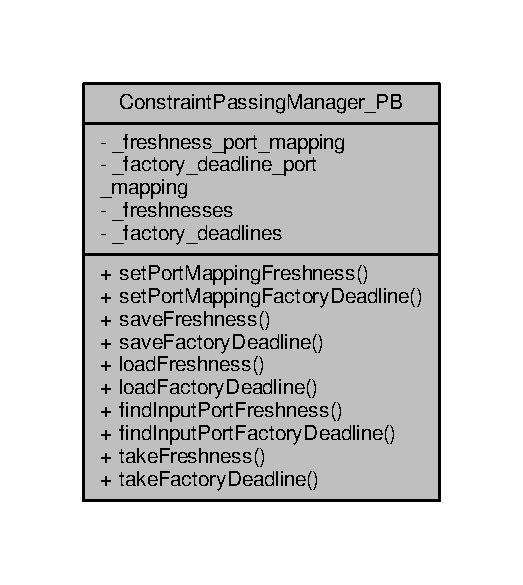
\includegraphics[width=251pt]{classConstraintPassingManager__PB__coll__graph}
\end{center}
\end{figure}
\subsection*{Public 멤버 함수}
\begin{DoxyCompactItemize}
\item 
void \hyperlink{classConstraintPassingManager__PB_a8da0b01c95f6eb6991ed763bc7151a0f}{set\+Port\+Mapping\+Freshness} (int inputport\+\_\+num, int outputport\+\_\+num)
\item 
void \hyperlink{classConstraintPassingManager__PB_a05e635543ffe3a2cd25c26c348812d09}{set\+Port\+Mapping\+Factory\+Deadline} (int inputport\+\_\+num, int outputport\+\_\+num)
\item 
void \hyperlink{classConstraintPassingManager__PB_ab1569a1c4dc95157e77ac43eed44e28a}{save\+Freshness} (int inputport\+\_\+num, int64\+\_\+t gentime)
\item 
void \hyperlink{classConstraintPassingManager__PB_af9984e913275a946bf4c8fb772f49225}{save\+Factory\+Deadline} (int inputport\+\_\+num, int64\+\_\+t duetime)
\item 
int64\+\_\+t \hyperlink{classConstraintPassingManager__PB_aaea8253b7002edd6272ae4ee36617566}{load\+Freshness} (int inputport\+\_\+num)
\item 
int64\+\_\+t \hyperlink{classConstraintPassingManager__PB_a10289fbb94c1b7d943e46ff814090805}{load\+Factory\+Deadline} (int inputport\+\_\+num)
\item 
int \hyperlink{classConstraintPassingManager__PB_addd726c7327487a745c64086574c6888}{find\+Input\+Port\+Freshness} (int outputport\+\_\+num)
\item 
int \hyperlink{classConstraintPassingManager__PB_aaf738795807249b71091a9155a2a838d}{find\+Input\+Port\+Factory\+Deadline} (int outputport\+\_\+num)
\item 
int64\+\_\+t \hyperlink{classConstraintPassingManager__PB_adac2cc79ac0b3f68d7a066bbae35486f}{take\+Freshness} (int outputport\+\_\+num)
\item 
int64\+\_\+t \hyperlink{classConstraintPassingManager__PB_a560d29d55761fbc597b6a694722ae665}{take\+Factory\+Deadline} (int outputport\+\_\+num)
\end{DoxyCompactItemize}
\subsection*{Private 속성}
\begin{DoxyCompactItemize}
\item 
std\+::bitset$<$ 5 $>$ \hyperlink{classConstraintPassingManager__PB_a34c12f7a79cb6c7a6c68bf63e17fed65}{\+\_\+freshness\+\_\+port\+\_\+mapping} \mbox{[}5\mbox{]}
\item 
std\+::bitset$<$ 5 $>$ \hyperlink{classConstraintPassingManager__PB_ac9c7c8ece56f6b66647da4793fdbcdd5}{\+\_\+factory\+\_\+deadline\+\_\+port\+\_\+mapping} \mbox{[}5\mbox{]}
\item 
int64\+\_\+t \hyperlink{classConstraintPassingManager__PB_ab06613fe88e472ed575a09e32d60bf67}{\+\_\+freshnesses} \mbox{[}5\mbox{]} = \{-\/1, -\/1, -\/1, -\/1, -\/1\}
\item 
int64\+\_\+t \hyperlink{classConstraintPassingManager__PB_a1a7e67da1e921de5f66eb9bf676ea945}{\+\_\+factory\+\_\+deadlines} \mbox{[}5\mbox{]} = \{-\/1, -\/1, -\/1, -\/1, -\/1\}
\end{DoxyCompactItemize}


\subsection{상세한 설명}
Pass two time constriant variables from input messages to output messages. 

\begin{DoxyRefDesc}{할일}
\item[\hyperlink{todo__todo000003}{할일}]modify every methods to correspond with new definition of message timestamp and deadline constraint \end{DoxyRefDesc}
\begin{DoxyAuthor}{작성자}
Beomjoon Yang 
\end{DoxyAuthor}
\begin{DoxyDate}{날짜}
2018-\/10-\/26 
\end{DoxyDate}
\begin{DoxyVersion}{버전}
0.\+0.\+1 
\end{DoxyVersion}


Processing\+\_\+block.\+cpp 파일의 200 번째 라인에서 정의되었습니다.



\subsection{멤버 함수 문서화}
\index{Constraint\+Passing\+Manager\+\_\+\+PB@{Constraint\+Passing\+Manager\+\_\+\+PB}!find\+Input\+Port\+Factory\+Deadline@{find\+Input\+Port\+Factory\+Deadline}}
\index{find\+Input\+Port\+Factory\+Deadline@{find\+Input\+Port\+Factory\+Deadline}!Constraint\+Passing\+Manager\+\_\+\+PB@{Constraint\+Passing\+Manager\+\_\+\+PB}}
\subsubsection[{\texorpdfstring{find\+Input\+Port\+Factory\+Deadline(int outputport\+\_\+num)}{findInputPortFactoryDeadline(int outputport_num)}}]{\setlength{\rightskip}{0pt plus 5cm}int Constraint\+Passing\+Manager\+\_\+\+P\+B\+::find\+Input\+Port\+Factory\+Deadline (
\begin{DoxyParamCaption}
\item[{int}]{outputport\+\_\+num}
\end{DoxyParamCaption}
)}\hypertarget{classConstraintPassingManager__PB_aaf738795807249b71091a9155a2a838d}{}\label{classConstraintPassingManager__PB_aaf738795807249b71091a9155a2a838d}


Processing\+\_\+block.\+cpp 파일의 281 번째 라인에서 정의되었습니다.

\index{Constraint\+Passing\+Manager\+\_\+\+PB@{Constraint\+Passing\+Manager\+\_\+\+PB}!find\+Input\+Port\+Freshness@{find\+Input\+Port\+Freshness}}
\index{find\+Input\+Port\+Freshness@{find\+Input\+Port\+Freshness}!Constraint\+Passing\+Manager\+\_\+\+PB@{Constraint\+Passing\+Manager\+\_\+\+PB}}
\subsubsection[{\texorpdfstring{find\+Input\+Port\+Freshness(int outputport\+\_\+num)}{findInputPortFreshness(int outputport_num)}}]{\setlength{\rightskip}{0pt plus 5cm}int Constraint\+Passing\+Manager\+\_\+\+P\+B\+::find\+Input\+Port\+Freshness (
\begin{DoxyParamCaption}
\item[{int}]{outputport\+\_\+num}
\end{DoxyParamCaption}
)}\hypertarget{classConstraintPassingManager__PB_addd726c7327487a745c64086574c6888}{}\label{classConstraintPassingManager__PB_addd726c7327487a745c64086574c6888}


Processing\+\_\+block.\+cpp 파일의 272 번째 라인에서 정의되었습니다.

\index{Constraint\+Passing\+Manager\+\_\+\+PB@{Constraint\+Passing\+Manager\+\_\+\+PB}!load\+Factory\+Deadline@{load\+Factory\+Deadline}}
\index{load\+Factory\+Deadline@{load\+Factory\+Deadline}!Constraint\+Passing\+Manager\+\_\+\+PB@{Constraint\+Passing\+Manager\+\_\+\+PB}}
\subsubsection[{\texorpdfstring{load\+Factory\+Deadline(int inputport\+\_\+num)}{loadFactoryDeadline(int inputport_num)}}]{\setlength{\rightskip}{0pt plus 5cm}int64\+\_\+t Constraint\+Passing\+Manager\+\_\+\+P\+B\+::load\+Factory\+Deadline (
\begin{DoxyParamCaption}
\item[{int}]{inputport\+\_\+num}
\end{DoxyParamCaption}
)}\hypertarget{classConstraintPassingManager__PB_a10289fbb94c1b7d943e46ff814090805}{}\label{classConstraintPassingManager__PB_a10289fbb94c1b7d943e46ff814090805}


Processing\+\_\+block.\+cpp 파일의 264 번째 라인에서 정의되었습니다.

\index{Constraint\+Passing\+Manager\+\_\+\+PB@{Constraint\+Passing\+Manager\+\_\+\+PB}!load\+Freshness@{load\+Freshness}}
\index{load\+Freshness@{load\+Freshness}!Constraint\+Passing\+Manager\+\_\+\+PB@{Constraint\+Passing\+Manager\+\_\+\+PB}}
\subsubsection[{\texorpdfstring{load\+Freshness(int inputport\+\_\+num)}{loadFreshness(int inputport_num)}}]{\setlength{\rightskip}{0pt plus 5cm}int64\+\_\+t Constraint\+Passing\+Manager\+\_\+\+P\+B\+::load\+Freshness (
\begin{DoxyParamCaption}
\item[{int}]{inputport\+\_\+num}
\end{DoxyParamCaption}
)}\hypertarget{classConstraintPassingManager__PB_aaea8253b7002edd6272ae4ee36617566}{}\label{classConstraintPassingManager__PB_aaea8253b7002edd6272ae4ee36617566}


Processing\+\_\+block.\+cpp 파일의 260 번째 라인에서 정의되었습니다.

\index{Constraint\+Passing\+Manager\+\_\+\+PB@{Constraint\+Passing\+Manager\+\_\+\+PB}!save\+Factory\+Deadline@{save\+Factory\+Deadline}}
\index{save\+Factory\+Deadline@{save\+Factory\+Deadline}!Constraint\+Passing\+Manager\+\_\+\+PB@{Constraint\+Passing\+Manager\+\_\+\+PB}}
\subsubsection[{\texorpdfstring{save\+Factory\+Deadline(int inputport\+\_\+num, int64\+\_\+t duetime)}{saveFactoryDeadline(int inputport_num, int64_t duetime)}}]{\setlength{\rightskip}{0pt plus 5cm}void Constraint\+Passing\+Manager\+\_\+\+P\+B\+::save\+Factory\+Deadline (
\begin{DoxyParamCaption}
\item[{int}]{inputport\+\_\+num, }
\item[{int64\+\_\+t}]{duetime}
\end{DoxyParamCaption}
)}\hypertarget{classConstraintPassingManager__PB_af9984e913275a946bf4c8fb772f49225}{}\label{classConstraintPassingManager__PB_af9984e913275a946bf4c8fb772f49225}


Processing\+\_\+block.\+cpp 파일의 251 번째 라인에서 정의되었습니다.

\index{Constraint\+Passing\+Manager\+\_\+\+PB@{Constraint\+Passing\+Manager\+\_\+\+PB}!save\+Freshness@{save\+Freshness}}
\index{save\+Freshness@{save\+Freshness}!Constraint\+Passing\+Manager\+\_\+\+PB@{Constraint\+Passing\+Manager\+\_\+\+PB}}
\subsubsection[{\texorpdfstring{save\+Freshness(int inputport\+\_\+num, int64\+\_\+t gentime)}{saveFreshness(int inputport_num, int64_t gentime)}}]{\setlength{\rightskip}{0pt plus 5cm}void Constraint\+Passing\+Manager\+\_\+\+P\+B\+::save\+Freshness (
\begin{DoxyParamCaption}
\item[{int}]{inputport\+\_\+num, }
\item[{int64\+\_\+t}]{gentime}
\end{DoxyParamCaption}
)}\hypertarget{classConstraintPassingManager__PB_ab1569a1c4dc95157e77ac43eed44e28a}{}\label{classConstraintPassingManager__PB_ab1569a1c4dc95157e77ac43eed44e28a}


Processing\+\_\+block.\+cpp 파일의 246 번째 라인에서 정의되었습니다.

\index{Constraint\+Passing\+Manager\+\_\+\+PB@{Constraint\+Passing\+Manager\+\_\+\+PB}!set\+Port\+Mapping\+Factory\+Deadline@{set\+Port\+Mapping\+Factory\+Deadline}}
\index{set\+Port\+Mapping\+Factory\+Deadline@{set\+Port\+Mapping\+Factory\+Deadline}!Constraint\+Passing\+Manager\+\_\+\+PB@{Constraint\+Passing\+Manager\+\_\+\+PB}}
\subsubsection[{\texorpdfstring{set\+Port\+Mapping\+Factory\+Deadline(int inputport\+\_\+num, int outputport\+\_\+num)}{setPortMappingFactoryDeadline(int inputport_num, int outputport_num)}}]{\setlength{\rightskip}{0pt plus 5cm}void Constraint\+Passing\+Manager\+\_\+\+P\+B\+::set\+Port\+Mapping\+Factory\+Deadline (
\begin{DoxyParamCaption}
\item[{int}]{inputport\+\_\+num, }
\item[{int}]{outputport\+\_\+num}
\end{DoxyParamCaption}
)}\hypertarget{classConstraintPassingManager__PB_a05e635543ffe3a2cd25c26c348812d09}{}\label{classConstraintPassingManager__PB_a05e635543ffe3a2cd25c26c348812d09}


Processing\+\_\+block.\+cpp 파일의 238 번째 라인에서 정의되었습니다.

\index{Constraint\+Passing\+Manager\+\_\+\+PB@{Constraint\+Passing\+Manager\+\_\+\+PB}!set\+Port\+Mapping\+Freshness@{set\+Port\+Mapping\+Freshness}}
\index{set\+Port\+Mapping\+Freshness@{set\+Port\+Mapping\+Freshness}!Constraint\+Passing\+Manager\+\_\+\+PB@{Constraint\+Passing\+Manager\+\_\+\+PB}}
\subsubsection[{\texorpdfstring{set\+Port\+Mapping\+Freshness(int inputport\+\_\+num, int outputport\+\_\+num)}{setPortMappingFreshness(int inputport_num, int outputport_num)}}]{\setlength{\rightskip}{0pt plus 5cm}void Constraint\+Passing\+Manager\+\_\+\+P\+B\+::set\+Port\+Mapping\+Freshness (
\begin{DoxyParamCaption}
\item[{int}]{inputport\+\_\+num, }
\item[{int}]{outputport\+\_\+num}
\end{DoxyParamCaption}
)}\hypertarget{classConstraintPassingManager__PB_a8da0b01c95f6eb6991ed763bc7151a0f}{}\label{classConstraintPassingManager__PB_a8da0b01c95f6eb6991ed763bc7151a0f}


Processing\+\_\+block.\+cpp 파일의 234 번째 라인에서 정의되었습니다.

\index{Constraint\+Passing\+Manager\+\_\+\+PB@{Constraint\+Passing\+Manager\+\_\+\+PB}!take\+Factory\+Deadline@{take\+Factory\+Deadline}}
\index{take\+Factory\+Deadline@{take\+Factory\+Deadline}!Constraint\+Passing\+Manager\+\_\+\+PB@{Constraint\+Passing\+Manager\+\_\+\+PB}}
\subsubsection[{\texorpdfstring{take\+Factory\+Deadline(int outputport\+\_\+num)}{takeFactoryDeadline(int outputport_num)}}]{\setlength{\rightskip}{0pt plus 5cm}int64\+\_\+t Constraint\+Passing\+Manager\+\_\+\+P\+B\+::take\+Factory\+Deadline (
\begin{DoxyParamCaption}
\item[{int}]{outputport\+\_\+num}
\end{DoxyParamCaption}
)}\hypertarget{classConstraintPassingManager__PB_a560d29d55761fbc597b6a694722ae665}{}\label{classConstraintPassingManager__PB_a560d29d55761fbc597b6a694722ae665}


Processing\+\_\+block.\+cpp 파일의 305 번째 라인에서 정의되었습니다.

\index{Constraint\+Passing\+Manager\+\_\+\+PB@{Constraint\+Passing\+Manager\+\_\+\+PB}!take\+Freshness@{take\+Freshness}}
\index{take\+Freshness@{take\+Freshness}!Constraint\+Passing\+Manager\+\_\+\+PB@{Constraint\+Passing\+Manager\+\_\+\+PB}}
\subsubsection[{\texorpdfstring{take\+Freshness(int outputport\+\_\+num)}{takeFreshness(int outputport_num)}}]{\setlength{\rightskip}{0pt plus 5cm}int64\+\_\+t Constraint\+Passing\+Manager\+\_\+\+P\+B\+::take\+Freshness (
\begin{DoxyParamCaption}
\item[{int}]{outputport\+\_\+num}
\end{DoxyParamCaption}
)}\hypertarget{classConstraintPassingManager__PB_adac2cc79ac0b3f68d7a066bbae35486f}{}\label{classConstraintPassingManager__PB_adac2cc79ac0b3f68d7a066bbae35486f}


Processing\+\_\+block.\+cpp 파일의 299 번째 라인에서 정의되었습니다.



\subsection{멤버 데이타 문서화}
\index{Constraint\+Passing\+Manager\+\_\+\+PB@{Constraint\+Passing\+Manager\+\_\+\+PB}!\+\_\+factory\+\_\+deadline\+\_\+port\+\_\+mapping@{\+\_\+factory\+\_\+deadline\+\_\+port\+\_\+mapping}}
\index{\+\_\+factory\+\_\+deadline\+\_\+port\+\_\+mapping@{\+\_\+factory\+\_\+deadline\+\_\+port\+\_\+mapping}!Constraint\+Passing\+Manager\+\_\+\+PB@{Constraint\+Passing\+Manager\+\_\+\+PB}}
\subsubsection[{\texorpdfstring{\+\_\+factory\+\_\+deadline\+\_\+port\+\_\+mapping}{_factory_deadline_port_mapping}}]{\setlength{\rightskip}{0pt plus 5cm}std\+::bitset$<$5$>$ Constraint\+Passing\+Manager\+\_\+\+P\+B\+::\+\_\+factory\+\_\+deadline\+\_\+port\+\_\+mapping\mbox{[}5\mbox{]}\hspace{0.3cm}{\ttfamily [private]}}\hypertarget{classConstraintPassingManager__PB_ac9c7c8ece56f6b66647da4793fdbcdd5}{}\label{classConstraintPassingManager__PB_ac9c7c8ece56f6b66647da4793fdbcdd5}


Processing\+\_\+block.\+cpp 파일의 225 번째 라인에서 정의되었습니다.

\index{Constraint\+Passing\+Manager\+\_\+\+PB@{Constraint\+Passing\+Manager\+\_\+\+PB}!\+\_\+factory\+\_\+deadlines@{\+\_\+factory\+\_\+deadlines}}
\index{\+\_\+factory\+\_\+deadlines@{\+\_\+factory\+\_\+deadlines}!Constraint\+Passing\+Manager\+\_\+\+PB@{Constraint\+Passing\+Manager\+\_\+\+PB}}
\subsubsection[{\texorpdfstring{\+\_\+factory\+\_\+deadlines}{_factory_deadlines}}]{\setlength{\rightskip}{0pt plus 5cm}int64\+\_\+t Constraint\+Passing\+Manager\+\_\+\+P\+B\+::\+\_\+factory\+\_\+deadlines\mbox{[}5\mbox{]} = \{-\/1, -\/1, -\/1, -\/1, -\/1\}\hspace{0.3cm}{\ttfamily [private]}}\hypertarget{classConstraintPassingManager__PB_a1a7e67da1e921de5f66eb9bf676ea945}{}\label{classConstraintPassingManager__PB_a1a7e67da1e921de5f66eb9bf676ea945}


Processing\+\_\+block.\+cpp 파일의 229 번째 라인에서 정의되었습니다.

\index{Constraint\+Passing\+Manager\+\_\+\+PB@{Constraint\+Passing\+Manager\+\_\+\+PB}!\+\_\+freshness\+\_\+port\+\_\+mapping@{\+\_\+freshness\+\_\+port\+\_\+mapping}}
\index{\+\_\+freshness\+\_\+port\+\_\+mapping@{\+\_\+freshness\+\_\+port\+\_\+mapping}!Constraint\+Passing\+Manager\+\_\+\+PB@{Constraint\+Passing\+Manager\+\_\+\+PB}}
\subsubsection[{\texorpdfstring{\+\_\+freshness\+\_\+port\+\_\+mapping}{_freshness_port_mapping}}]{\setlength{\rightskip}{0pt plus 5cm}std\+::bitset$<$5$>$ Constraint\+Passing\+Manager\+\_\+\+P\+B\+::\+\_\+freshness\+\_\+port\+\_\+mapping\mbox{[}5\mbox{]}\hspace{0.3cm}{\ttfamily [private]}}\hypertarget{classConstraintPassingManager__PB_a34c12f7a79cb6c7a6c68bf63e17fed65}{}\label{classConstraintPassingManager__PB_a34c12f7a79cb6c7a6c68bf63e17fed65}


Processing\+\_\+block.\+cpp 파일의 224 번째 라인에서 정의되었습니다.

\index{Constraint\+Passing\+Manager\+\_\+\+PB@{Constraint\+Passing\+Manager\+\_\+\+PB}!\+\_\+freshnesses@{\+\_\+freshnesses}}
\index{\+\_\+freshnesses@{\+\_\+freshnesses}!Constraint\+Passing\+Manager\+\_\+\+PB@{Constraint\+Passing\+Manager\+\_\+\+PB}}
\subsubsection[{\texorpdfstring{\+\_\+freshnesses}{_freshnesses}}]{\setlength{\rightskip}{0pt plus 5cm}int64\+\_\+t Constraint\+Passing\+Manager\+\_\+\+P\+B\+::\+\_\+freshnesses\mbox{[}5\mbox{]} = \{-\/1, -\/1, -\/1, -\/1, -\/1\}\hspace{0.3cm}{\ttfamily [private]}}\hypertarget{classConstraintPassingManager__PB_ab06613fe88e472ed575a09e32d60bf67}{}\label{classConstraintPassingManager__PB_ab06613fe88e472ed575a09e32d60bf67}


Processing\+\_\+block.\+cpp 파일의 228 번째 라인에서 정의되었습니다.



이 클래스에 대한 문서화 페이지는 다음의 파일로부터 생성되었습니다.\+:\begin{DoxyCompactItemize}
\item 
src/\hyperlink{Processing__block_8cpp}{Processing\+\_\+block.\+cpp}\end{DoxyCompactItemize}

\hypertarget{classDeadlineMonitor__Fac}{}\section{Deadline\+Monitor\+\_\+\+Fac}
\label{classDeadlineMonitor__Fac}\index{Deadline\+Monitor\+\_\+\+Fac@{Deadline\+Monitor\+\_\+\+Fac}}


Deadline\+Monitor\+\_\+\+Fac에 대한 협력 다이어그램\+:\nopagebreak
\begin{figure}[H]
\begin{center}
\leavevmode
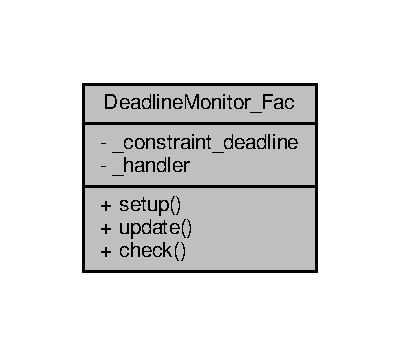
\includegraphics[width=192pt]{classDeadlineMonitor__Fac__coll__graph}
\end{center}
\end{figure}
\subsection*{Public 멤버 함수}
\begin{DoxyCompactItemize}
\item 
void \hyperlink{classDeadlineMonitor__Fac_acc97e655dbcbafb1ae421d6097f700c5}{setup} (int64\+\_\+t deadline, void($\ast$\hyperlink{sample__main_8cpp_ae298e0b16475a05fd3d021c2daf90062}{deadline\+\_\+handler})())
\item 
void \hyperlink{classDeadlineMonitor__Fac_a1302d302e9ec205bf409722523560de8}{update} (int64\+\_\+t $\ast$msg\+\_\+duetime)
\item 
int \hyperlink{classDeadlineMonitor__Fac_ad4b3d5ac9779fe651cfe432a95a6051b}{check} (int64\+\_\+t msg\+\_\+duetime, int64\+\_\+t current\+\_\+time)
\end{DoxyCompactItemize}
\subsection*{Private 속성}
\begin{DoxyCompactItemize}
\item 
int64\+\_\+t \hyperlink{classDeadlineMonitor__Fac_a8fe1a647054d4ead7e9d41869bef0234}{\+\_\+constraint\+\_\+deadline} = -\/1
\item 
void($\ast$ \hyperlink{classDeadlineMonitor__Fac_ae36ff128554a0ba47cbcca57543586bb}{\+\_\+handler} )()
\end{DoxyCompactItemize}


\subsection{상세한 설명}


Factory.\+cpp 파일의 46 번째 라인에서 정의되었습니다.



\subsection{멤버 함수 문서화}
\index{Deadline\+Monitor\+\_\+\+Fac@{Deadline\+Monitor\+\_\+\+Fac}!check@{check}}
\index{check@{check}!Deadline\+Monitor\+\_\+\+Fac@{Deadline\+Monitor\+\_\+\+Fac}}
\subsubsection[{\texorpdfstring{check(int64\+\_\+t msg\+\_\+duetime, int64\+\_\+t current\+\_\+time)}{check(int64_t msg_duetime, int64_t current_time)}}]{\setlength{\rightskip}{0pt plus 5cm}int Deadline\+Monitor\+\_\+\+Fac\+::check (
\begin{DoxyParamCaption}
\item[{int64\+\_\+t}]{msg\+\_\+duetime, }
\item[{int64\+\_\+t}]{current\+\_\+time}
\end{DoxyParamCaption}
)}\hypertarget{classDeadlineMonitor__Fac_ad4b3d5ac9779fe651cfe432a95a6051b}{}\label{classDeadlineMonitor__Fac_ad4b3d5ac9779fe651cfe432a95a6051b}


Factory.\+cpp 파일의 67 번째 라인에서 정의되었습니다.



다음을 참조함 \+:  \+\_\+constraint\+\_\+deadline, \+\_\+handler.



다음에 의해서 참조됨 \+:  Factory$<$ Data\+\_\+0, Data\+\_\+1, Data\+\_\+2, Data\+\_\+3, Data\+\_\+4, Data\+\_\+5, Data\+\_\+6, Data\+\_\+7, Data\+\_\+8, Data\+\_\+9 $>$\+::check\+Deadline().



이 함수를 호출하는 함수들에 대한 그래프입니다.\+:\nopagebreak
\begin{figure}[H]
\begin{center}
\leavevmode
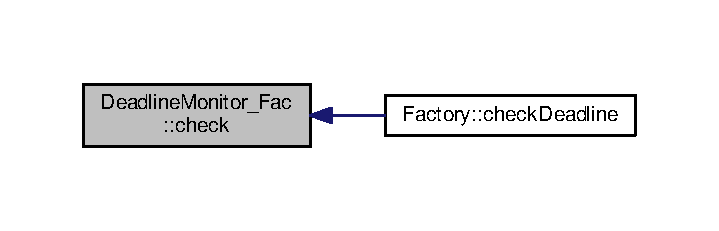
\includegraphics[width=345pt]{classDeadlineMonitor__Fac_ad4b3d5ac9779fe651cfe432a95a6051b_icgraph}
\end{center}
\end{figure}


\index{Deadline\+Monitor\+\_\+\+Fac@{Deadline\+Monitor\+\_\+\+Fac}!setup@{setup}}
\index{setup@{setup}!Deadline\+Monitor\+\_\+\+Fac@{Deadline\+Monitor\+\_\+\+Fac}}
\subsubsection[{\texorpdfstring{setup(int64\+\_\+t deadline, void($\ast$deadline\+\_\+handler)())}{setup(int64_t deadline, void(*deadline_handler)())}}]{\setlength{\rightskip}{0pt plus 5cm}void Deadline\+Monitor\+\_\+\+Fac\+::setup (
\begin{DoxyParamCaption}
\item[{int64\+\_\+t}]{deadline, }
\item[{void($\ast$)()}]{deadline\+\_\+handler}
\end{DoxyParamCaption}
)}\hypertarget{classDeadlineMonitor__Fac_acc97e655dbcbafb1ae421d6097f700c5}{}\label{classDeadlineMonitor__Fac_acc97e655dbcbafb1ae421d6097f700c5}


Factory.\+cpp 파일의 57 번째 라인에서 정의되었습니다.



다음을 참조함 \+:  \+\_\+constraint\+\_\+deadline, \+\_\+handler, deadline\+\_\+handler().



다음에 의해서 참조됨 \+:  Factory$<$ Data\+\_\+0, Data\+\_\+1, Data\+\_\+2, Data\+\_\+3, Data\+\_\+4, Data\+\_\+5, Data\+\_\+6, Data\+\_\+7, Data\+\_\+8, Data\+\_\+9 $>$\+::set\+Deadline().



이 함수 내부에서 호출하는 함수들에 대한 그래프입니다.\+:\nopagebreak
\begin{figure}[H]
\begin{center}
\leavevmode
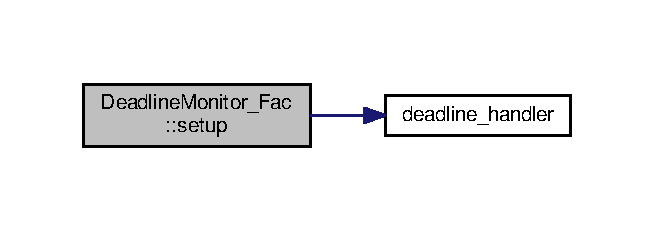
\includegraphics[width=314pt]{classDeadlineMonitor__Fac_acc97e655dbcbafb1ae421d6097f700c5_cgraph}
\end{center}
\end{figure}




이 함수를 호출하는 함수들에 대한 그래프입니다.\+:\nopagebreak
\begin{figure}[H]
\begin{center}
\leavevmode
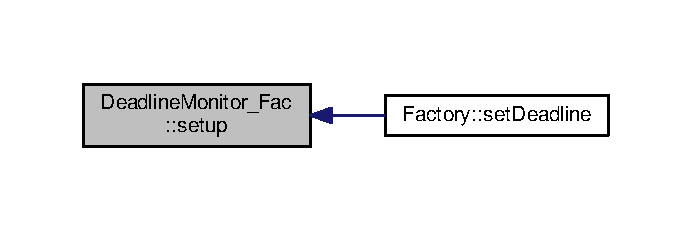
\includegraphics[width=332pt]{classDeadlineMonitor__Fac_acc97e655dbcbafb1ae421d6097f700c5_icgraph}
\end{center}
\end{figure}


\index{Deadline\+Monitor\+\_\+\+Fac@{Deadline\+Monitor\+\_\+\+Fac}!update@{update}}
\index{update@{update}!Deadline\+Monitor\+\_\+\+Fac@{Deadline\+Monitor\+\_\+\+Fac}}
\subsubsection[{\texorpdfstring{update(int64\+\_\+t $\ast$msg\+\_\+duetime)}{update(int64_t *msg_duetime)}}]{\setlength{\rightskip}{0pt plus 5cm}void Deadline\+Monitor\+\_\+\+Fac\+::update (
\begin{DoxyParamCaption}
\item[{int64\+\_\+t $\ast$}]{msg\+\_\+duetime}
\end{DoxyParamCaption}
)}\hypertarget{classDeadlineMonitor__Fac_a1302d302e9ec205bf409722523560de8}{}\label{classDeadlineMonitor__Fac_a1302d302e9ec205bf409722523560de8}


Factory.\+cpp 파일의 62 번째 라인에서 정의되었습니다.



다음을 참조함 \+:  \+\_\+constraint\+\_\+deadline, System\+Clock\+::get\+Current\+Time().



다음에 의해서 참조됨 \+:  Factory$<$ Data\+\_\+0, Data\+\_\+1, Data\+\_\+2, Data\+\_\+3, Data\+\_\+4, Data\+\_\+5, Data\+\_\+6, Data\+\_\+7, Data\+\_\+8, Data\+\_\+9 $>$\+::update\+Deadline\+F\+I\+P().



이 함수 내부에서 호출하는 함수들에 대한 그래프입니다.\+:\nopagebreak
\begin{figure}[H]
\begin{center}
\leavevmode
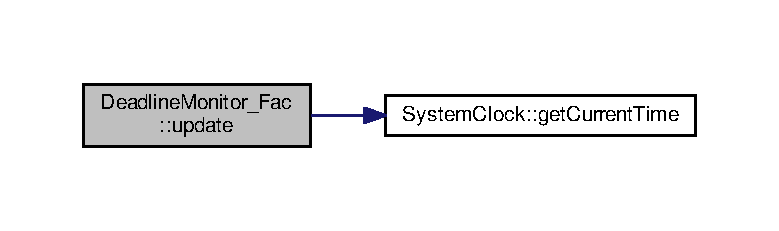
\includegraphics[width=350pt]{classDeadlineMonitor__Fac_a1302d302e9ec205bf409722523560de8_cgraph}
\end{center}
\end{figure}




이 함수를 호출하는 함수들에 대한 그래프입니다.\+:\nopagebreak
\begin{figure}[H]
\begin{center}
\leavevmode
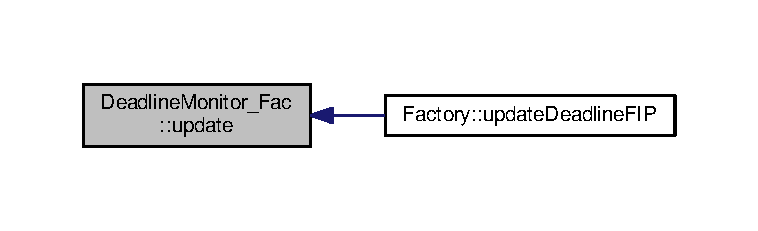
\includegraphics[width=350pt]{classDeadlineMonitor__Fac_a1302d302e9ec205bf409722523560de8_icgraph}
\end{center}
\end{figure}




\subsection{멤버 데이타 문서화}
\index{Deadline\+Monitor\+\_\+\+Fac@{Deadline\+Monitor\+\_\+\+Fac}!\+\_\+constraint\+\_\+deadline@{\+\_\+constraint\+\_\+deadline}}
\index{\+\_\+constraint\+\_\+deadline@{\+\_\+constraint\+\_\+deadline}!Deadline\+Monitor\+\_\+\+Fac@{Deadline\+Monitor\+\_\+\+Fac}}
\subsubsection[{\texorpdfstring{\+\_\+constraint\+\_\+deadline}{_constraint_deadline}}]{\setlength{\rightskip}{0pt plus 5cm}int64\+\_\+t Deadline\+Monitor\+\_\+\+Fac\+::\+\_\+constraint\+\_\+deadline = -\/1\hspace{0.3cm}{\ttfamily [private]}}\hypertarget{classDeadlineMonitor__Fac_a8fe1a647054d4ead7e9d41869bef0234}{}\label{classDeadlineMonitor__Fac_a8fe1a647054d4ead7e9d41869bef0234}


Factory.\+cpp 파일의 52 번째 라인에서 정의되었습니다.



다음에 의해서 참조됨 \+:  check(), setup(), update().

\index{Deadline\+Monitor\+\_\+\+Fac@{Deadline\+Monitor\+\_\+\+Fac}!\+\_\+handler@{\+\_\+handler}}
\index{\+\_\+handler@{\+\_\+handler}!Deadline\+Monitor\+\_\+\+Fac@{Deadline\+Monitor\+\_\+\+Fac}}
\subsubsection[{\texorpdfstring{\+\_\+handler}{_handler}}]{\setlength{\rightskip}{0pt plus 5cm}void($\ast$ Deadline\+Monitor\+\_\+\+Fac\+::\+\_\+handler) ()\hspace{0.3cm}{\ttfamily [private]}}\hypertarget{classDeadlineMonitor__Fac_ae36ff128554a0ba47cbcca57543586bb}{}\label{classDeadlineMonitor__Fac_ae36ff128554a0ba47cbcca57543586bb}


Factory.\+cpp 파일의 53 번째 라인에서 정의되었습니다.



다음에 의해서 참조됨 \+:  check(), Input\+Rate\+Monitor\+\_\+\+Fac$<$ data\+\_\+t $>$\+::check(), Output\+Rate\+Monitor\+\_\+\+Fac$<$ data\+\_\+t $>$\+::check(), setup(), Input\+Rate\+Monitor\+\_\+\+Fac$<$ data\+\_\+t $>$\+::setup(), Output\+Rate\+Monitor\+\_\+\+Fac$<$ data\+\_\+t $>$\+::setup().



이 클래스에 대한 문서화 페이지는 다음의 파일로부터 생성되었습니다.\+:\begin{DoxyCompactItemize}
\item 
src/\hyperlink{Factory_8cpp}{Factory.\+cpp}\end{DoxyCompactItemize}

\hypertarget{classDeadlineMonitor__PB}{}\section{Deadline\+Monitor\+\_\+\+PB}
\label{classDeadlineMonitor__PB}\index{Deadline\+Monitor\+\_\+\+PB@{Deadline\+Monitor\+\_\+\+PB}}


Detect deadline constraint violation.  




Deadline\+Monitor\+\_\+\+P\+B에 대한 협력 다이어그램\+:\nopagebreak
\begin{figure}[H]
\begin{center}
\leavevmode
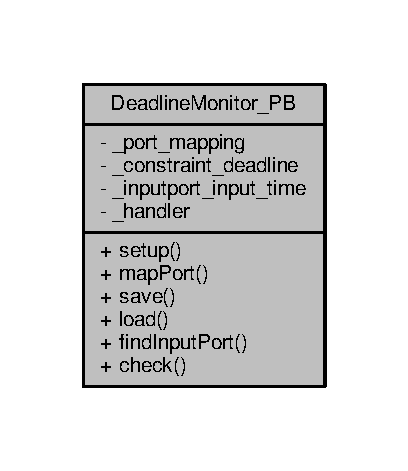
\includegraphics[width=196pt]{classDeadlineMonitor__PB__coll__graph}
\end{center}
\end{figure}
\subsection*{Public 멤버 함수}
\begin{DoxyCompactItemize}
\item 
void \hyperlink{classDeadlineMonitor__PB_a6456b87d4c185b8a974f71cc7e729d83}{setup} (int64\+\_\+t deadline, void($\ast$\hyperlink{sample__main_8cpp_ae298e0b16475a05fd3d021c2daf90062}{deadline\+\_\+handler})())
\item 
void \hyperlink{classDeadlineMonitor__PB_a9e1fb5351877e803ba40357fff46d19a}{map\+Port} (int inputport\+\_\+num, int outputport\+\_\+num)
\item 
void \hyperlink{classDeadlineMonitor__PB_aa100310cce2b5c63a13edc18d38483e4}{save} (int inputport\+\_\+num)
\item 
int64\+\_\+t \hyperlink{classDeadlineMonitor__PB_aa438c96cf364469c2da17070d358cd09}{load} (int inputport\+\_\+num)
\item 
int \hyperlink{classDeadlineMonitor__PB_aa42200d62a805c2bf6eaeb7eb3841305}{find\+Input\+Port} (int outputport\+\_\+num)
\item 
int \hyperlink{classDeadlineMonitor__PB_a7debcade9bbf07add3752aa980bc3b19}{check} (int intputport\+\_\+num)
\end{DoxyCompactItemize}
\subsection*{Private 속성}
\begin{DoxyCompactItemize}
\item 
std\+::bitset$<$ 5 $>$ \hyperlink{classDeadlineMonitor__PB_a86839dadce69f56fba6589355b56513d}{\+\_\+port\+\_\+mapping} \mbox{[}5\mbox{]}
\item 
int64\+\_\+t \hyperlink{classDeadlineMonitor__PB_a4aff480c381c68671213b6c3779bb137}{\+\_\+constraint\+\_\+deadline} = -\/1
\item 
int64\+\_\+t \hyperlink{classDeadlineMonitor__PB_af11957e5aef255a6be8fb21f2f3719d7}{\+\_\+inputport\+\_\+input\+\_\+time} \mbox{[}5\mbox{]}
\item 
void($\ast$ \hyperlink{classDeadlineMonitor__PB_a637df7fb7c75351ea967d45c64f3af13}{\+\_\+handler} )()
\end{DoxyCompactItemize}


\subsection{상세한 설명}
Detect deadline constraint violation. 

\begin{DoxyRefDesc}{할일}
\item[\hyperlink{todo__todo000002}{할일}]modify \hyperlink{classDeadlineMonitor__PB_a6456b87d4c185b8a974f71cc7e729d83}{setup()} and \hyperlink{classDeadlineMonitor__PB_a7debcade9bbf07add3752aa980bc3b19}{check()} to correspond with new definition of message timestamp and deadline constraint \end{DoxyRefDesc}
\begin{DoxyAuthor}{작성자}
Beomjoon Yang 
\end{DoxyAuthor}
\begin{DoxyDate}{날짜}
2018-\/10-\/26 
\end{DoxyDate}
\begin{DoxyVersion}{버전}
0.\+0.\+1 
\end{DoxyVersion}


Processing\+\_\+block.\+cpp 파일의 129 번째 라인에서 정의되었습니다.



\subsection{멤버 함수 문서화}
\index{Deadline\+Monitor\+\_\+\+PB@{Deadline\+Monitor\+\_\+\+PB}!check@{check}}
\index{check@{check}!Deadline\+Monitor\+\_\+\+PB@{Deadline\+Monitor\+\_\+\+PB}}
\subsubsection[{\texorpdfstring{check(int intputport\+\_\+num)}{check(int intputport_num)}}]{\setlength{\rightskip}{0pt plus 5cm}int Deadline\+Monitor\+\_\+\+P\+B\+::check (
\begin{DoxyParamCaption}
\item[{int}]{intputport\+\_\+num}
\end{DoxyParamCaption}
)}\hypertarget{classDeadlineMonitor__PB_a7debcade9bbf07add3752aa980bc3b19}{}\label{classDeadlineMonitor__PB_a7debcade9bbf07add3752aa980bc3b19}


Processing\+\_\+block.\+cpp 파일의 173 번째 라인에서 정의되었습니다.



다음을 참조함 \+:  System\+Clock\+::get\+Current\+Time().



이 함수 내부에서 호출하는 함수들에 대한 그래프입니다.\+:\nopagebreak
\begin{figure}[H]
\begin{center}
\leavevmode
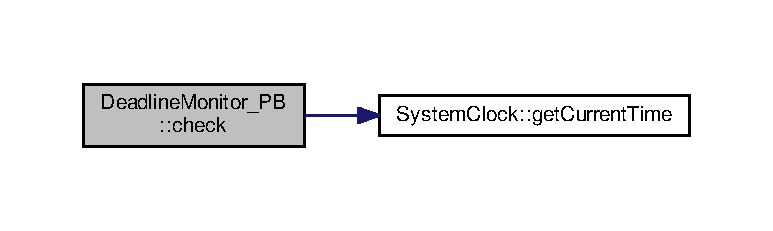
\includegraphics[width=350pt]{classDeadlineMonitor__PB_a7debcade9bbf07add3752aa980bc3b19_cgraph}
\end{center}
\end{figure}


\index{Deadline\+Monitor\+\_\+\+PB@{Deadline\+Monitor\+\_\+\+PB}!find\+Input\+Port@{find\+Input\+Port}}
\index{find\+Input\+Port@{find\+Input\+Port}!Deadline\+Monitor\+\_\+\+PB@{Deadline\+Monitor\+\_\+\+PB}}
\subsubsection[{\texorpdfstring{find\+Input\+Port(int outputport\+\_\+num)}{findInputPort(int outputport_num)}}]{\setlength{\rightskip}{0pt plus 5cm}int Deadline\+Monitor\+\_\+\+P\+B\+::find\+Input\+Port (
\begin{DoxyParamCaption}
\item[{int}]{outputport\+\_\+num}
\end{DoxyParamCaption}
)}\hypertarget{classDeadlineMonitor__PB_aa42200d62a805c2bf6eaeb7eb3841305}{}\label{classDeadlineMonitor__PB_aa42200d62a805c2bf6eaeb7eb3841305}


Processing\+\_\+block.\+cpp 파일의 164 번째 라인에서 정의되었습니다.

\index{Deadline\+Monitor\+\_\+\+PB@{Deadline\+Monitor\+\_\+\+PB}!load@{load}}
\index{load@{load}!Deadline\+Monitor\+\_\+\+PB@{Deadline\+Monitor\+\_\+\+PB}}
\subsubsection[{\texorpdfstring{load(int inputport\+\_\+num)}{load(int inputport_num)}}]{\setlength{\rightskip}{0pt plus 5cm}int64\+\_\+t Deadline\+Monitor\+\_\+\+P\+B\+::load (
\begin{DoxyParamCaption}
\item[{int}]{inputport\+\_\+num}
\end{DoxyParamCaption}
)}\hypertarget{classDeadlineMonitor__PB_aa438c96cf364469c2da17070d358cd09}{}\label{classDeadlineMonitor__PB_aa438c96cf364469c2da17070d358cd09}


Processing\+\_\+block.\+cpp 파일의 160 번째 라인에서 정의되었습니다.

\index{Deadline\+Monitor\+\_\+\+PB@{Deadline\+Monitor\+\_\+\+PB}!map\+Port@{map\+Port}}
\index{map\+Port@{map\+Port}!Deadline\+Monitor\+\_\+\+PB@{Deadline\+Monitor\+\_\+\+PB}}
\subsubsection[{\texorpdfstring{map\+Port(int inputport\+\_\+num, int outputport\+\_\+num)}{mapPort(int inputport_num, int outputport_num)}}]{\setlength{\rightskip}{0pt plus 5cm}void Deadline\+Monitor\+\_\+\+P\+B\+::map\+Port (
\begin{DoxyParamCaption}
\item[{int}]{inputport\+\_\+num, }
\item[{int}]{outputport\+\_\+num}
\end{DoxyParamCaption}
)}\hypertarget{classDeadlineMonitor__PB_a9e1fb5351877e803ba40357fff46d19a}{}\label{classDeadlineMonitor__PB_a9e1fb5351877e803ba40357fff46d19a}


Processing\+\_\+block.\+cpp 파일의 150 번째 라인에서 정의되었습니다.

\index{Deadline\+Monitor\+\_\+\+PB@{Deadline\+Monitor\+\_\+\+PB}!save@{save}}
\index{save@{save}!Deadline\+Monitor\+\_\+\+PB@{Deadline\+Monitor\+\_\+\+PB}}
\subsubsection[{\texorpdfstring{save(int inputport\+\_\+num)}{save(int inputport_num)}}]{\setlength{\rightskip}{0pt plus 5cm}void Deadline\+Monitor\+\_\+\+P\+B\+::save (
\begin{DoxyParamCaption}
\item[{int}]{inputport\+\_\+num}
\end{DoxyParamCaption}
)}\hypertarget{classDeadlineMonitor__PB_aa100310cce2b5c63a13edc18d38483e4}{}\label{classDeadlineMonitor__PB_aa100310cce2b5c63a13edc18d38483e4}


Processing\+\_\+block.\+cpp 파일의 154 번째 라인에서 정의되었습니다.



다음을 참조함 \+:  System\+Clock\+::get\+Current\+Time().



이 함수 내부에서 호출하는 함수들에 대한 그래프입니다.\+:\nopagebreak
\begin{figure}[H]
\begin{center}
\leavevmode
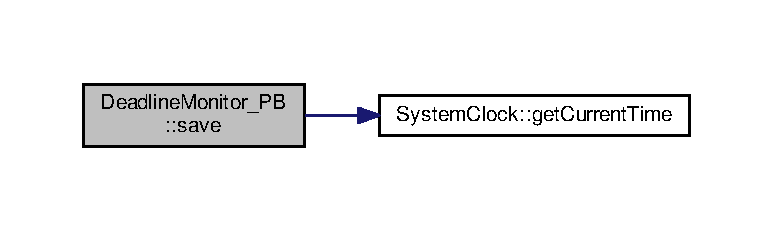
\includegraphics[width=350pt]{classDeadlineMonitor__PB_aa100310cce2b5c63a13edc18d38483e4_cgraph}
\end{center}
\end{figure}


\index{Deadline\+Monitor\+\_\+\+PB@{Deadline\+Monitor\+\_\+\+PB}!setup@{setup}}
\index{setup@{setup}!Deadline\+Monitor\+\_\+\+PB@{Deadline\+Monitor\+\_\+\+PB}}
\subsubsection[{\texorpdfstring{setup(int64\+\_\+t deadline, void($\ast$deadline\+\_\+handler)())}{setup(int64_t deadline, void(*deadline_handler)())}}]{\setlength{\rightskip}{0pt plus 5cm}void Deadline\+Monitor\+\_\+\+P\+B\+::setup (
\begin{DoxyParamCaption}
\item[{int64\+\_\+t}]{deadline, }
\item[{void($\ast$)()}]{deadline\+\_\+handler}
\end{DoxyParamCaption}
)}\hypertarget{classDeadlineMonitor__PB_a6456b87d4c185b8a974f71cc7e729d83}{}\label{classDeadlineMonitor__PB_a6456b87d4c185b8a974f71cc7e729d83}


Processing\+\_\+block.\+cpp 파일의 145 번째 라인에서 정의되었습니다.



다음을 참조함 \+:  deadline\+\_\+handler().



이 함수 내부에서 호출하는 함수들에 대한 그래프입니다.\+:\nopagebreak
\begin{figure}[H]
\begin{center}
\leavevmode
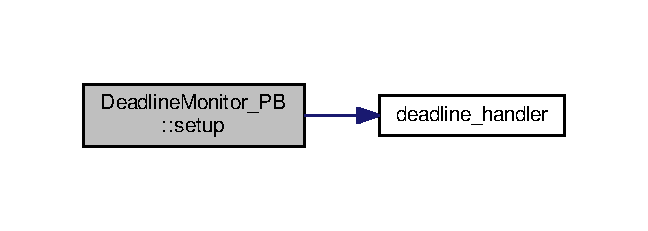
\includegraphics[width=311pt]{classDeadlineMonitor__PB_a6456b87d4c185b8a974f71cc7e729d83_cgraph}
\end{center}
\end{figure}




\subsection{멤버 데이타 문서화}
\index{Deadline\+Monitor\+\_\+\+PB@{Deadline\+Monitor\+\_\+\+PB}!\+\_\+constraint\+\_\+deadline@{\+\_\+constraint\+\_\+deadline}}
\index{\+\_\+constraint\+\_\+deadline@{\+\_\+constraint\+\_\+deadline}!Deadline\+Monitor\+\_\+\+PB@{Deadline\+Monitor\+\_\+\+PB}}
\subsubsection[{\texorpdfstring{\+\_\+constraint\+\_\+deadline}{_constraint_deadline}}]{\setlength{\rightskip}{0pt plus 5cm}int64\+\_\+t Deadline\+Monitor\+\_\+\+P\+B\+::\+\_\+constraint\+\_\+deadline = -\/1\hspace{0.3cm}{\ttfamily [private]}}\hypertarget{classDeadlineMonitor__PB_a4aff480c381c68671213b6c3779bb137}{}\label{classDeadlineMonitor__PB_a4aff480c381c68671213b6c3779bb137}


Processing\+\_\+block.\+cpp 파일의 140 번째 라인에서 정의되었습니다.

\index{Deadline\+Monitor\+\_\+\+PB@{Deadline\+Monitor\+\_\+\+PB}!\+\_\+handler@{\+\_\+handler}}
\index{\+\_\+handler@{\+\_\+handler}!Deadline\+Monitor\+\_\+\+PB@{Deadline\+Monitor\+\_\+\+PB}}
\subsubsection[{\texorpdfstring{\+\_\+handler}{_handler}}]{\setlength{\rightskip}{0pt plus 5cm}void($\ast$ Deadline\+Monitor\+\_\+\+P\+B\+::\+\_\+handler) ()\hspace{0.3cm}{\ttfamily [private]}}\hypertarget{classDeadlineMonitor__PB_a637df7fb7c75351ea967d45c64f3af13}{}\label{classDeadlineMonitor__PB_a637df7fb7c75351ea967d45c64f3af13}


Processing\+\_\+block.\+cpp 파일의 142 번째 라인에서 정의되었습니다.

\index{Deadline\+Monitor\+\_\+\+PB@{Deadline\+Monitor\+\_\+\+PB}!\+\_\+inputport\+\_\+input\+\_\+time@{\+\_\+inputport\+\_\+input\+\_\+time}}
\index{\+\_\+inputport\+\_\+input\+\_\+time@{\+\_\+inputport\+\_\+input\+\_\+time}!Deadline\+Monitor\+\_\+\+PB@{Deadline\+Monitor\+\_\+\+PB}}
\subsubsection[{\texorpdfstring{\+\_\+inputport\+\_\+input\+\_\+time}{_inputport_input_time}}]{\setlength{\rightskip}{0pt plus 5cm}int64\+\_\+t Deadline\+Monitor\+\_\+\+P\+B\+::\+\_\+inputport\+\_\+input\+\_\+time\mbox{[}5\mbox{]}\hspace{0.3cm}{\ttfamily [private]}}\hypertarget{classDeadlineMonitor__PB_af11957e5aef255a6be8fb21f2f3719d7}{}\label{classDeadlineMonitor__PB_af11957e5aef255a6be8fb21f2f3719d7}


Processing\+\_\+block.\+cpp 파일의 141 번째 라인에서 정의되었습니다.

\index{Deadline\+Monitor\+\_\+\+PB@{Deadline\+Monitor\+\_\+\+PB}!\+\_\+port\+\_\+mapping@{\+\_\+port\+\_\+mapping}}
\index{\+\_\+port\+\_\+mapping@{\+\_\+port\+\_\+mapping}!Deadline\+Monitor\+\_\+\+PB@{Deadline\+Monitor\+\_\+\+PB}}
\subsubsection[{\texorpdfstring{\+\_\+port\+\_\+mapping}{_port_mapping}}]{\setlength{\rightskip}{0pt plus 5cm}std\+::bitset$<$5$>$ Deadline\+Monitor\+\_\+\+P\+B\+::\+\_\+port\+\_\+mapping\mbox{[}5\mbox{]}\hspace{0.3cm}{\ttfamily [private]}}\hypertarget{classDeadlineMonitor__PB_a86839dadce69f56fba6589355b56513d}{}\label{classDeadlineMonitor__PB_a86839dadce69f56fba6589355b56513d}


Processing\+\_\+block.\+cpp 파일의 139 번째 라인에서 정의되었습니다.



이 클래스에 대한 문서화 페이지는 다음의 파일로부터 생성되었습니다.\+:\begin{DoxyCompactItemize}
\item 
src/\hyperlink{Processing__block_8cpp}{Processing\+\_\+block.\+cpp}\end{DoxyCompactItemize}

\hypertarget{classEventDataPort__PB}{}\section{Event\+Data\+Port\+\_\+\+PB$<$ Data\+\_\+0, Data\+\_\+1, Data\+\_\+2, Data\+\_\+3, Data\+\_\+4, Data\+\_\+5, Data\+\_\+6, Data\+\_\+7, Data\+\_\+8, Data\+\_\+9 $>$}
\label{classEventDataPort__PB}\index{Event\+Data\+Port\+\_\+\+P\+B$<$ Data\+\_\+0, Data\+\_\+1, Data\+\_\+2, Data\+\_\+3, Data\+\_\+4, Data\+\_\+5, Data\+\_\+6, Data\+\_\+7, Data\+\_\+8, Data\+\_\+9 $>$@{Event\+Data\+Port\+\_\+\+P\+B$<$ Data\+\_\+0, Data\+\_\+1, Data\+\_\+2, Data\+\_\+3, Data\+\_\+4, Data\+\_\+5, Data\+\_\+6, Data\+\_\+7, Data\+\_\+8, Data\+\_\+9 $>$}}


{\ttfamily \#include $<$Processing\+\_\+block\+\_\+references.\+h$>$}



Event\+Data\+Port\+\_\+\+PB$<$ Data\+\_\+0, Data\+\_\+1, Data\+\_\+2, Data\+\_\+3, Data\+\_\+4, Data\+\_\+5, Data\+\_\+6, Data\+\_\+7, Data\+\_\+8, Data\+\_\+9 $>$에 대한 협력 다이어그램\+:\nopagebreak
\begin{figure}[H]
\begin{center}
\leavevmode
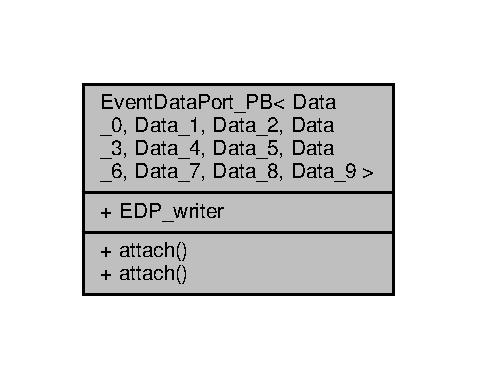
\includegraphics[width=229pt]{classEventDataPort__PB__coll__graph}
\end{center}
\end{figure}
\subsection*{Public 멤버 함수}
\begin{DoxyCompactItemize}
\item 
int \hyperlink{classEventDataPort__PB_a9cf59d5a3d5b1963433965aa04550b5d}{attach} (\hyperlink{classProcessingBlock}{Processing\+Block}$<$ Data\+\_\+0, Data\+\_\+1, Data\+\_\+2, Data\+\_\+3, Data\+\_\+4, Data\+\_\+5, Data\+\_\+6, Data\+\_\+7, Data\+\_\+8, Data\+\_\+9 $>$ $\ast$, std\+::string)
\item 
int \hyperlink{classEventDataPort__PB_a9cf59d5a3d5b1963433965aa04550b5d}{attach} (\hyperlink{classProcessingBlock}{Processing\+Block}$<$ Data\+\_\+0, Data\+\_\+1, Data\+\_\+2, Data\+\_\+3, Data\+\_\+4, Data\+\_\+5, Data\+\_\+6, Data\+\_\+7, Data\+\_\+8, Data\+\_\+9 $>$ $\ast$, std\+::string)
\end{DoxyCompactItemize}
\subsection*{Public 속성}
\begin{DoxyCompactItemize}
\item 
dds\+::pub\+::\+Data\+Writer$<$ int $>$ $\ast$ \hyperlink{classEventDataPort__PB_af4f01ada6acf6d431c9d8e799f9b1ad0}{E\+D\+P\+\_\+writer}
\end{DoxyCompactItemize}


\subsection{상세한 설명}
\subsubsection*{template$<$typename Data\+\_\+0, typename Data\+\_\+1, typename Data\+\_\+2, typename Data\+\_\+3, typename Data\+\_\+4, typename Data\+\_\+5, typename Data\+\_\+6, typename Data\+\_\+7, typename Data\+\_\+8, typename Data\+\_\+9$>$\\*
class Event\+Data\+Port\+\_\+\+P\+B$<$ Data\+\_\+0, Data\+\_\+1, Data\+\_\+2, Data\+\_\+3, Data\+\_\+4, Data\+\_\+5, Data\+\_\+6, Data\+\_\+7, Data\+\_\+8, Data\+\_\+9 $>$}



Base\+\_\+cell.\+cpp 파일의 32 번째 라인에서 정의되었습니다.



\subsection{멤버 함수 문서화}
\index{Event\+Data\+Port\+\_\+\+PB@{Event\+Data\+Port\+\_\+\+PB}!attach@{attach}}
\index{attach@{attach}!Event\+Data\+Port\+\_\+\+PB@{Event\+Data\+Port\+\_\+\+PB}}
\subsubsection[{\texorpdfstring{attach(\+Processing\+Block$<$ Data\+\_\+0, Data\+\_\+1, Data\+\_\+2, Data\+\_\+3, Data\+\_\+4, Data\+\_\+5, Data\+\_\+6, Data\+\_\+7, Data\+\_\+8, Data\+\_\+9 $>$ $\ast$, std\+::string)}{attach(ProcessingBlock< Data_0, Data_1, Data_2, Data_3, Data_4, Data_5, Data_6, Data_7, Data_8, Data_9 > *, std::string)}}]{\setlength{\rightskip}{0pt plus 5cm}template$<$typename Data\+\_\+0 , typename Data\+\_\+1 , typename Data\+\_\+2 , typename Data\+\_\+3 , typename Data\+\_\+4 , typename Data\+\_\+5 , typename Data\+\_\+6 , typename Data\+\_\+7 , typename Data\+\_\+8 , typename Data\+\_\+9 $>$ int {\bf Event\+Data\+Port\+\_\+\+PB}$<$ Data\+\_\+0, Data\+\_\+1, Data\+\_\+2, Data\+\_\+3, Data\+\_\+4, Data\+\_\+5, Data\+\_\+6, Data\+\_\+7, Data\+\_\+8, Data\+\_\+9 $>$\+::attach (
\begin{DoxyParamCaption}
\item[{{\bf Processing\+Block}$<$ Data\+\_\+0, Data\+\_\+1, Data\+\_\+2, Data\+\_\+3, Data\+\_\+4, Data\+\_\+5, Data\+\_\+6, Data\+\_\+7, Data\+\_\+8, Data\+\_\+9 $>$ $\ast$}]{, }
\item[{std\+::string}]{}
\end{DoxyParamCaption}
)}\hypertarget{classEventDataPort__PB_a9cf59d5a3d5b1963433965aa04550b5d}{}\label{classEventDataPort__PB_a9cf59d5a3d5b1963433965aa04550b5d}
\index{Event\+Data\+Port\+\_\+\+PB@{Event\+Data\+Port\+\_\+\+PB}!attach@{attach}}
\index{attach@{attach}!Event\+Data\+Port\+\_\+\+PB@{Event\+Data\+Port\+\_\+\+PB}}
\subsubsection[{\texorpdfstring{attach(\+Processing\+Block$<$ Data\+\_\+0, Data\+\_\+1, Data\+\_\+2, Data\+\_\+3, Data\+\_\+4, Data\+\_\+5, Data\+\_\+6, Data\+\_\+7, Data\+\_\+8, Data\+\_\+9 $>$ $\ast$, std\+::string)}{attach(ProcessingBlock< Data_0, Data_1, Data_2, Data_3, Data_4, Data_5, Data_6, Data_7, Data_8, Data_9 > *, std::string)}}]{\setlength{\rightskip}{0pt plus 5cm}template$<$typename Data\+\_\+0 , typename Data\+\_\+1 , typename Data\+\_\+2 , typename Data\+\_\+3 , typename Data\+\_\+4 , typename Data\+\_\+5 , typename Data\+\_\+6 , typename Data\+\_\+7 , typename Data\+\_\+8 , typename Data\+\_\+9 $>$ int {\bf Event\+Data\+Port\+\_\+\+PB}$<$ Data\+\_\+0, Data\+\_\+1, Data\+\_\+2, Data\+\_\+3, Data\+\_\+4, Data\+\_\+5, Data\+\_\+6, Data\+\_\+7, Data\+\_\+8, Data\+\_\+9 $>$\+::attach (
\begin{DoxyParamCaption}
\item[{{\bf Processing\+Block}$<$ Data\+\_\+0, Data\+\_\+1, Data\+\_\+2, Data\+\_\+3, Data\+\_\+4, Data\+\_\+5, Data\+\_\+6, Data\+\_\+7, Data\+\_\+8, Data\+\_\+9 $>$ $\ast$}]{PB, }
\item[{std\+::string}]{topic}
\end{DoxyParamCaption}
)}\hypertarget{classEventDataPort__PB_a9cf59d5a3d5b1963433965aa04550b5d}{}\label{classEventDataPort__PB_a9cf59d5a3d5b1963433965aa04550b5d}


Base\+\_\+cell.\+cpp 파일의 450 번째 라인에서 정의되었습니다.



다음을 참조함 \+:  Processing\+Block$<$ Data\+\_\+0, Data\+\_\+1, Data\+\_\+2, Data\+\_\+3, Data\+\_\+4, Data\+\_\+5, Data\+\_\+6, Data\+\_\+7, Data\+\_\+8, Data\+\_\+9 $>$\+::\+E\+DP, Processing\+Block$<$ Data\+\_\+0, Data\+\_\+1, Data\+\_\+2, Data\+\_\+3, Data\+\_\+4, Data\+\_\+5, Data\+\_\+6, Data\+\_\+7, Data\+\_\+8, Data\+\_\+9 $>$\+::topic\+\_\+event.



\subsection{멤버 데이타 문서화}
\index{Event\+Data\+Port\+\_\+\+PB@{Event\+Data\+Port\+\_\+\+PB}!E\+D\+P\+\_\+writer@{E\+D\+P\+\_\+writer}}
\index{E\+D\+P\+\_\+writer@{E\+D\+P\+\_\+writer}!Event\+Data\+Port\+\_\+\+PB@{Event\+Data\+Port\+\_\+\+PB}}
\subsubsection[{\texorpdfstring{E\+D\+P\+\_\+writer}{EDP_writer}}]{\setlength{\rightskip}{0pt plus 5cm}template$<$typename Data\+\_\+0 , typename Data\+\_\+1 , typename Data\+\_\+2 , typename Data\+\_\+3 , typename Data\+\_\+4 , typename Data\+\_\+5 , typename Data\+\_\+6 , typename Data\+\_\+7 , typename Data\+\_\+8 , typename Data\+\_\+9 $>$ dds\+::pub\+::\+Data\+Writer$<$ int $>$ $\ast$ {\bf Event\+Data\+Port\+\_\+\+PB}$<$ Data\+\_\+0, Data\+\_\+1, Data\+\_\+2, Data\+\_\+3, Data\+\_\+4, Data\+\_\+5, Data\+\_\+6, Data\+\_\+7, Data\+\_\+8, Data\+\_\+9 $>$\+::E\+D\+P\+\_\+writer}\hypertarget{classEventDataPort__PB_af4f01ada6acf6d431c9d8e799f9b1ad0}{}\label{classEventDataPort__PB_af4f01ada6acf6d431c9d8e799f9b1ad0}


Base\+\_\+cell.\+cpp 파일의 438 번째 라인에서 정의되었습니다.



이 클래스에 대한 문서화 페이지는 다음의 파일들로부터 생성되었습니다.\+:\begin{DoxyCompactItemize}
\item 
src/\hyperlink{Base__cell_8cpp}{Base\+\_\+cell.\+cpp}\item 
src/\hyperlink{Processing__block__references_8h}{Processing\+\_\+block\+\_\+references.\+h}\end{DoxyCompactItemize}

\hypertarget{classFactory}{}\section{Factory$<$ Data\+\_\+0, Data\+\_\+1, Data\+\_\+2, Data\+\_\+3, Data\+\_\+4, Data\+\_\+5, Data\+\_\+6, Data\+\_\+7, Data\+\_\+8, Data\+\_\+9 $>$}
\label{classFactory}\index{Factory$<$ Data\+\_\+0, Data\+\_\+1, Data\+\_\+2, Data\+\_\+3, Data\+\_\+4, Data\+\_\+5, Data\+\_\+6, Data\+\_\+7, Data\+\_\+8, Data\+\_\+9 $>$@{Factory$<$ Data\+\_\+0, Data\+\_\+1, Data\+\_\+2, Data\+\_\+3, Data\+\_\+4, Data\+\_\+5, Data\+\_\+6, Data\+\_\+7, Data\+\_\+8, Data\+\_\+9 $>$}}


Splash Language\+Constructs $>$ Component\+Type $>$ Factory\+Type.  




Factory$<$ Data\+\_\+0, Data\+\_\+1, Data\+\_\+2, Data\+\_\+3, Data\+\_\+4, Data\+\_\+5, Data\+\_\+6, Data\+\_\+7, Data\+\_\+8, Data\+\_\+9 $>$에 대한 협력 다이어그램\+:\nopagebreak
\begin{figure}[H]
\begin{center}
\leavevmode
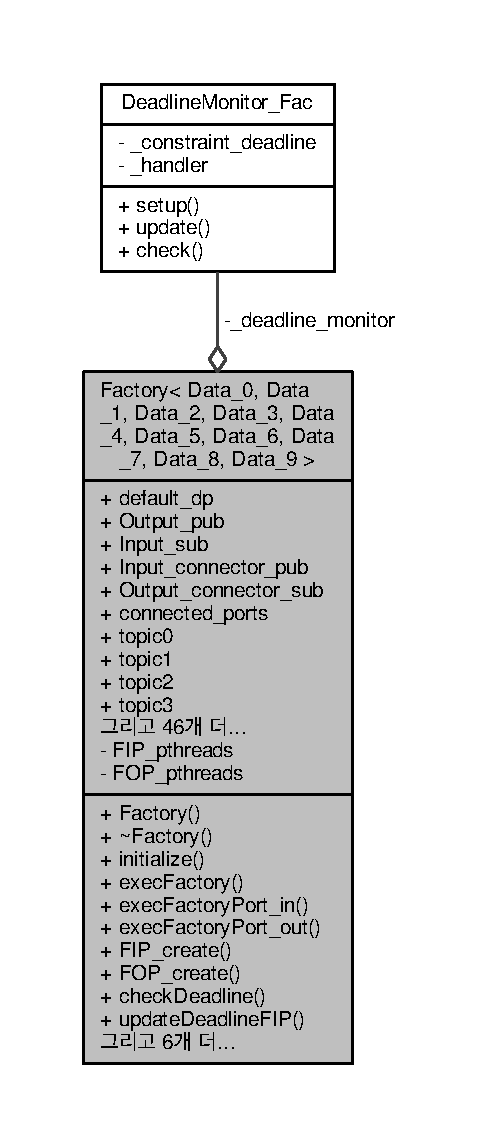
\includegraphics[height=550pt]{classFactory__coll__graph}
\end{center}
\end{figure}
\subsection*{Public 멤버 함수}
\begin{DoxyCompactItemize}
\item 
\hyperlink{classFactory_a213338063efff7dd723b05ef6b71fde3}{Factory} ()
\item 
\hyperlink{classFactory_aadae14f3339b510c3a82bcb7c77d7262}{$\sim$\+Factory} ()
\item 
void \hyperlink{classFactory_a64a97c299b156747868846be05ad9257}{initialize} (std\+::string name, int64\+\_\+t deadline, void($\ast$\hyperlink{sample__main_8cpp_ae298e0b16475a05fd3d021c2daf90062}{deadline\+\_\+handler})(), int node\+\_\+id, int core\+\_\+id)
\item 
void \hyperlink{classFactory_a500058128cac41fd5fd45aac1a8f3d7d}{exec\+Factory} (std\+::vector$<$ const char $\ast$ $>$ atomic\+\_\+list)
\item 
void \hyperlink{classFactory_a6ffc6624a41ccd66f6ba05b696e50211}{exec\+Factory\+Port\+\_\+in} ()
\item 
void \hyperlink{classFactory_a26be38da40eb21a04b0b4712282518e9}{exec\+Factory\+Port\+\_\+out} ()
\item 
void \hyperlink{classFactory_a83757b0ec4d4c3f1e6c1df0cbca2a5d9}{F\+I\+P\+\_\+create} (const int port\+\_\+id)
\item 
void \hyperlink{classFactory_a37a09c78d3bf8fb3df5ece85bace2733}{F\+O\+P\+\_\+create} (const int port\+\_\+id)
\item 
void \hyperlink{classFactory_a7f2a51ac39c034ccc0923eaa39cff780}{check\+Deadline} (int64\+\_\+t msg\+\_\+duetime)
\item 
void \hyperlink{classFactory_a5982eaac979b3ef080244ddc5007b690}{update\+Deadline\+F\+IP} (int64\+\_\+t $\ast$msg\+\_\+duetime)
\item 
void \hyperlink{classFactory_a0777c31e360f6c08f9069482501e3a70}{update\+Deadline\+F\+OP} (int64\+\_\+t $\ast$msg\+\_\+duetime)
\item 
void \hyperlink{classFactory_ab884eec61738ee5f0fcf7d25a4855bc0}{set\+Deadline} (int64\+\_\+t deadline, void($\ast$\hyperlink{sample__main_8cpp_ae298e0b16475a05fd3d021c2daf90062}{deadline\+\_\+handler})())
\item 
void \hyperlink{classFactory_af9ced939952de12016774d0225c93520}{initialize} (std\+::string, double, int, int)
\item 
void \hyperlink{classFactory_aef23e931404b99e10ae4d9b8723e24a6}{exec\+Factory} (std\+::vector$<$ char $\ast$ $>$ atomic\+\_\+list)
\item 
void \hyperlink{classFactory_a6ffc6624a41ccd66f6ba05b696e50211}{exec\+Factory\+Port\+\_\+in} ()
\item 
void \hyperlink{classFactory_a26be38da40eb21a04b0b4712282518e9}{exec\+Factory\+Port\+\_\+out} ()
\end{DoxyCompactItemize}
\subsection*{Public 속성}
\begin{DoxyCompactItemize}
\item 
dds\+::domain\+::\+Domain\+Participant \hyperlink{classFactory_a7e8eac562d69cbed38ee27137c860498}{default\+\_\+dp} \{org\+::opensplice\+::domain\+::default\+\_\+id()\}
\item 
dds\+::pub\+::\+Publisher \hyperlink{classFactory_a6a48290339d13731e356940e7d29db00}{Output\+\_\+pub} \{\hyperlink{classFactory_a7e8eac562d69cbed38ee27137c860498}{default\+\_\+dp}, default\+\_\+dp.\+default\+\_\+publisher\+\_\+qos()\}
\item 
dds\+::sub\+::\+Subscriber \hyperlink{classFactory_a1c96bbf37ab7ad1775854d283298212a}{Input\+\_\+sub} \{\hyperlink{classFactory_a7e8eac562d69cbed38ee27137c860498}{default\+\_\+dp}, default\+\_\+dp.\+default\+\_\+subscriber\+\_\+qos()\}
\item 
dds\+::pub\+::\+Publisher \hyperlink{classFactory_a0fa1e401cba8537d6aff6a5b1ef34637}{Input\+\_\+connector\+\_\+pub} \{\hyperlink{classFactory_a7e8eac562d69cbed38ee27137c860498}{default\+\_\+dp}, default\+\_\+dp.\+default\+\_\+publisher\+\_\+qos()\}
\item 
dds\+::sub\+::\+Subscriber \hyperlink{classFactory_a2b0fe17e9fe543b0dc41c3898293ae3e}{Output\+\_\+connector\+\_\+sub} \{\hyperlink{classFactory_a7e8eac562d69cbed38ee27137c860498}{default\+\_\+dp}, default\+\_\+dp.\+default\+\_\+subscriber\+\_\+qos()\}
\item 
std\+::bitset$<$ 10 $>$ \hyperlink{classFactory_a47d1a95acef574eae4410faf891130df}{connected\+\_\+ports}
\item 
dds\+::topic\+::\+Topic$<$ Data\+\_\+0 $>$ $\ast$ \hyperlink{classFactory_a575dfe382a4cbf779aa8b141fb38f2c4}{topic0}
\item 
dds\+::topic\+::\+Topic$<$ Data\+\_\+1 $>$ $\ast$ \hyperlink{classFactory_a0dfe2257a4968511148b107030387e25}{topic1}
\item 
dds\+::topic\+::\+Topic$<$ Data\+\_\+2 $>$ $\ast$ \hyperlink{classFactory_ab9a453fcd33f6843819c86ffa569a46a}{topic2}
\item 
dds\+::topic\+::\+Topic$<$ Data\+\_\+3 $>$ $\ast$ \hyperlink{classFactory_a54fef646f78840de831f09c0f4f065c9}{topic3}
\item 
dds\+::topic\+::\+Topic$<$ Data\+\_\+4 $>$ $\ast$ \hyperlink{classFactory_a9621c03dc6ffd5d7c1b73c66f37cae7c}{topic4}
\item 
dds\+::topic\+::\+Topic$<$ Data\+\_\+5 $>$ $\ast$ \hyperlink{classFactory_a81ba9f3ce496974146df61fb932a64e1}{topic5}
\item 
dds\+::topic\+::\+Topic$<$ Data\+\_\+6 $>$ $\ast$ \hyperlink{classFactory_a9ead1fa2f7352def150a5789f7c47b33}{topic6}
\item 
dds\+::topic\+::\+Topic$<$ Data\+\_\+7 $>$ $\ast$ \hyperlink{classFactory_af496c7d2b15f70cd42cfe0ce20e0656c}{topic7}
\item 
dds\+::topic\+::\+Topic$<$ Data\+\_\+8 $>$ $\ast$ \hyperlink{classFactory_a9357b99e6b5b07bb4115b854010873fd}{topic8}
\item 
dds\+::topic\+::\+Topic$<$ Data\+\_\+9 $>$ $\ast$ \hyperlink{classFactory_a6f4d710cdaab90dc87a0fff6cd3a34bc}{topic9}
\item 
dds\+::topic\+::\+Topic$<$ Data\+\_\+0 $>$ $\ast$ \hyperlink{classFactory_a292d6100f4cee20be6f5f7b5f1ed13b5}{connector\+\_\+topic0}
\item 
dds\+::topic\+::\+Topic$<$ Data\+\_\+1 $>$ $\ast$ \hyperlink{classFactory_a744afdb2e49dc636774fdd4a2f6ec2d1}{connector\+\_\+topic1}
\item 
dds\+::topic\+::\+Topic$<$ Data\+\_\+2 $>$ $\ast$ \hyperlink{classFactory_ac7074f7a4d429bacd720150a248dc0e3}{connector\+\_\+topic2}
\item 
dds\+::topic\+::\+Topic$<$ Data\+\_\+3 $>$ $\ast$ \hyperlink{classFactory_a637aec1cd43fdfb430f59858e6408a6e}{connector\+\_\+topic3}
\item 
dds\+::topic\+::\+Topic$<$ Data\+\_\+4 $>$ $\ast$ \hyperlink{classFactory_a89e5876a2d5f8d4c48fe48023450a8cc}{connector\+\_\+topic4}
\item 
dds\+::topic\+::\+Topic$<$ Data\+\_\+5 $>$ $\ast$ \hyperlink{classFactory_abb59b6717eb779f8cf2dfdab552319cc}{connector\+\_\+topic5}
\item 
dds\+::topic\+::\+Topic$<$ Data\+\_\+6 $>$ $\ast$ \hyperlink{classFactory_a92c01f1de5c207d812509de1ca687bea}{connector\+\_\+topic6}
\item 
dds\+::topic\+::\+Topic$<$ Data\+\_\+7 $>$ $\ast$ \hyperlink{classFactory_a40529b00720b7f40615b07d0fb2265b3}{connector\+\_\+topic7}
\item 
dds\+::topic\+::\+Topic$<$ Data\+\_\+8 $>$ $\ast$ \hyperlink{classFactory_a567cf4a6f03c8dd9be6cf26f6fd277d5}{connector\+\_\+topic8}
\item 
dds\+::topic\+::\+Topic$<$ Data\+\_\+9 $>$ $\ast$ \hyperlink{classFactory_adffa083b38163d0e5b912250cb27cb58}{connector\+\_\+topic9}
\item 
std\+::vector$<$ dds\+::sub\+::\+Sample$<$ Data\+\_\+0 $>$ $>$ \hyperlink{classFactory_a126e4ae222ac36e61cb29c93d7b375b3}{input\+\_\+data\+\_\+1} \{1\}
\item 
std\+::vector$<$ dds\+::sub\+::\+Sample$<$ Data\+\_\+0 $>$ $>$\+::iterator \hyperlink{classFactory_afe81300eda34ff9d60fc4f243b94534d}{iter\+\_\+1} = input\+\_\+data\+\_\+1.\+begin()
\item 
std\+::vector$<$ dds\+::sub\+::\+Sample$<$ Data\+\_\+1 $>$ $>$ \hyperlink{classFactory_af23053102c7edeb254b91930647ed3e7}{input\+\_\+data\+\_\+2} \{1\}
\item 
std\+::vector$<$ dds\+::sub\+::\+Sample$<$ Data\+\_\+1 $>$ $>$\+::iterator \hyperlink{classFactory_a018adc4b2d04e5ed2f71dca5261a353e}{iter\+\_\+2} = input\+\_\+data\+\_\+2.\+begin()
\item 
std\+::vector$<$ dds\+::sub\+::\+Sample$<$ Data\+\_\+2 $>$ $>$ \hyperlink{classFactory_af87769552e1c9b6b4f910eb992f23f9f}{input\+\_\+data\+\_\+3} \{1\}
\item 
std\+::vector$<$ dds\+::sub\+::\+Sample$<$ Data\+\_\+2 $>$ $>$\+::iterator \hyperlink{classFactory_adbd632440369980117032c2ba154eadb}{iter\+\_\+3} = input\+\_\+data\+\_\+3.\+begin()
\item 
std\+::vector$<$ dds\+::sub\+::\+Sample$<$ Data\+\_\+3 $>$ $>$ \hyperlink{classFactory_a4bad31e0b189b22dfc4c1127b06040e0}{input\+\_\+data\+\_\+4} \{1\}
\item 
std\+::vector$<$ dds\+::sub\+::\+Sample$<$ Data\+\_\+3 $>$ $>$\+::iterator \hyperlink{classFactory_acd5df27b9212689ac21bba1db77eaf1f}{iter\+\_\+4} = input\+\_\+data\+\_\+4.\+begin()
\item 
std\+::vector$<$ dds\+::sub\+::\+Sample$<$ Data\+\_\+4 $>$ $>$ \hyperlink{classFactory_a6aa6f19a951657809ad1663af4597670}{input\+\_\+data\+\_\+5} \{1\}
\item 
std\+::vector$<$ dds\+::sub\+::\+Sample$<$ Data\+\_\+4 $>$ $>$\+::iterator \hyperlink{classFactory_a6122d3e9df3241c7ce971675402efc25}{iter\+\_\+5} = input\+\_\+data\+\_\+5.\+begin()
\item 
std\+::vector$<$ dds\+::sub\+::\+Sample$<$ Data\+\_\+5 $>$ $>$ \hyperlink{classFactory_a5b0446916aba039e366098c8db768b72}{output\+\_\+connector\+\_\+data\+\_\+1} \{1\}
\item 
std\+::vector$<$ dds\+::sub\+::\+Sample$<$ Data\+\_\+5 $>$ $>$\+::iterator \hyperlink{classFactory_a560460eae381287c085b613c5330dadd}{connector\+\_\+iter\+\_\+1}
\item 
std\+::vector$<$ dds\+::sub\+::\+Sample$<$ Data\+\_\+6 $>$ $>$ \hyperlink{classFactory_a9f636cd7fe32df0bd19e4ec9490d5ccd}{output\+\_\+connector\+\_\+data\+\_\+2} \{1\}
\item 
std\+::vector$<$ dds\+::sub\+::\+Sample$<$ Data\+\_\+6 $>$ $>$\+::iterator \hyperlink{classFactory_acb10615bebab1e5eda677a8b41c0fd29}{connector\+\_\+iter\+\_\+2}
\item 
std\+::vector$<$ dds\+::sub\+::\+Sample$<$ Data\+\_\+7 $>$ $>$ \hyperlink{classFactory_acb470e6e5293ed45c2a1284015b8a63f}{output\+\_\+connector\+\_\+data\+\_\+3} \{1\}
\item 
std\+::vector$<$ dds\+::sub\+::\+Sample$<$ Data\+\_\+7 $>$ $>$\+::iterator \hyperlink{classFactory_abe759623a3ab82ecd6ae3923629c397d}{connector\+\_\+iter\+\_\+3}
\item 
std\+::vector$<$ dds\+::sub\+::\+Sample$<$ Data\+\_\+8 $>$ $>$ \hyperlink{classFactory_add95efaac04f798e826ac10668d38e48}{output\+\_\+connector\+\_\+data\+\_\+4} \{1\}
\item 
std\+::vector$<$ dds\+::sub\+::\+Sample$<$ Data\+\_\+8 $>$ $>$\+::iterator \hyperlink{classFactory_aa664c801aed2472266996c3e3256c406}{connector\+\_\+iter\+\_\+4}
\item 
std\+::vector$<$ dds\+::sub\+::\+Sample$<$ Data\+\_\+9 $>$ $>$ \hyperlink{classFactory_ae8ed17f677db9e6c55b3f75379baf818}{output\+\_\+connector\+\_\+data\+\_\+5} \{1\}
\item 
std\+::vector$<$ dds\+::sub\+::\+Sample$<$ Data\+\_\+9 $>$ $>$\+::iterator \hyperlink{classFactory_addefc1a08fde4845b9d68bd9c0743f94}{connector\+\_\+iter\+\_\+5}
\item 
\hyperlink{classInputDataPort__Fac}{Input\+Data\+Port\+\_\+\+Fac}$<$ Data\+\_\+0, Data\+\_\+1, Data\+\_\+2, Data\+\_\+3, Data\+\_\+4, Data\+\_\+5, Data\+\_\+6, Data\+\_\+7, Data\+\_\+8, Data\+\_\+9 $>$ $\ast$ \hyperlink{classFactory_ae0d8f03ec007e2da61fbc59840193256}{I\+D\+P0}
\item 
\hyperlink{classInputDataPort__Fac}{Input\+Data\+Port\+\_\+\+Fac}$<$ Data\+\_\+0, Data\+\_\+1, Data\+\_\+2, Data\+\_\+3, Data\+\_\+4, Data\+\_\+5, Data\+\_\+6, Data\+\_\+7, Data\+\_\+8, Data\+\_\+9 $>$ $\ast$ \hyperlink{classFactory_a52571611c058145431671afaedee6db3}{I\+D\+P1}
\item 
\hyperlink{classInputDataPort__Fac}{Input\+Data\+Port\+\_\+\+Fac}$<$ Data\+\_\+0, Data\+\_\+1, Data\+\_\+2, Data\+\_\+3, Data\+\_\+4, Data\+\_\+5, Data\+\_\+6, Data\+\_\+7, Data\+\_\+8, Data\+\_\+9 $>$ $\ast$ \hyperlink{classFactory_a41dabc989ec1d1e8889e94627b73d4c7}{I\+D\+P2}
\item 
\hyperlink{classInputDataPort__Fac}{Input\+Data\+Port\+\_\+\+Fac}$<$ Data\+\_\+0, Data\+\_\+1, Data\+\_\+2, Data\+\_\+3, Data\+\_\+4, Data\+\_\+5, Data\+\_\+6, Data\+\_\+7, Data\+\_\+8, Data\+\_\+9 $>$ $\ast$ \hyperlink{classFactory_a67c4448f7c694be4e12739d2d3cd7910}{I\+D\+P3}
\item 
\hyperlink{classInputDataPort__Fac}{Input\+Data\+Port\+\_\+\+Fac}$<$ Data\+\_\+0, Data\+\_\+1, Data\+\_\+2, Data\+\_\+3, Data\+\_\+4, Data\+\_\+5, Data\+\_\+6, Data\+\_\+7, Data\+\_\+8, Data\+\_\+9 $>$ $\ast$ \hyperlink{classFactory_a965146b854acde70e6a7ca1095e44526}{I\+D\+P4}
\item 
\hyperlink{classOutputDataPort__Fac}{Output\+Data\+Port\+\_\+\+Fac}$<$ Data\+\_\+0, Data\+\_\+1, Data\+\_\+2, Data\+\_\+3, Data\+\_\+4, Data\+\_\+5, Data\+\_\+6, Data\+\_\+7, Data\+\_\+8, Data\+\_\+9 $>$ $\ast$ \hyperlink{classFactory_a3644b51b1cfbe7385523ab9f08dac1a6}{O\+D\+P0}
\item 
\hyperlink{classOutputDataPort__Fac}{Output\+Data\+Port\+\_\+\+Fac}$<$ Data\+\_\+0, Data\+\_\+1, Data\+\_\+2, Data\+\_\+3, Data\+\_\+4, Data\+\_\+5, Data\+\_\+6, Data\+\_\+7, Data\+\_\+8, Data\+\_\+9 $>$ $\ast$ \hyperlink{classFactory_a15fbd1b09238bdd01967b10fd20136d8}{O\+D\+P1}
\item 
\hyperlink{classOutputDataPort__Fac}{Output\+Data\+Port\+\_\+\+Fac}$<$ Data\+\_\+0, Data\+\_\+1, Data\+\_\+2, Data\+\_\+3, Data\+\_\+4, Data\+\_\+5, Data\+\_\+6, Data\+\_\+7, Data\+\_\+8, Data\+\_\+9 $>$ $\ast$ \hyperlink{classFactory_a1a6a173fb03250b269320d772fb0855a}{O\+D\+P2}
\item 
\hyperlink{classOutputDataPort__Fac}{Output\+Data\+Port\+\_\+\+Fac}$<$ Data\+\_\+0, Data\+\_\+1, Data\+\_\+2, Data\+\_\+3, Data\+\_\+4, Data\+\_\+5, Data\+\_\+6, Data\+\_\+7, Data\+\_\+8, Data\+\_\+9 $>$ $\ast$ \hyperlink{classFactory_a0b72fe47a8a15af6f9dfdeb46c4bc3fc}{O\+D\+P3}
\item 
\hyperlink{classOutputDataPort__Fac}{Output\+Data\+Port\+\_\+\+Fac}$<$ Data\+\_\+0, Data\+\_\+1, Data\+\_\+2, Data\+\_\+3, Data\+\_\+4, Data\+\_\+5, Data\+\_\+6, Data\+\_\+7, Data\+\_\+8, Data\+\_\+9 $>$ $\ast$ \hyperlink{classFactory_a3a94566e0097a4f38401c0d7d11750b1}{O\+D\+P4}
\end{DoxyCompactItemize}
\subsection*{Private 속성}
\begin{DoxyCompactItemize}
\item 
std\+::vector$<$ std\+::thread $\ast$ $>$ \hyperlink{classFactory_a10eeb0e3620d248a5f500ab923e1bd4c}{F\+I\+P\+\_\+pthreads}
\item 
std\+::vector$<$ std\+::thread $\ast$ $>$ \hyperlink{classFactory_adef777708bab91c0dc6a20eba43c3e1e}{F\+O\+P\+\_\+pthreads}
\item 
\hyperlink{classDeadlineMonitor__Fac}{Deadline\+Monitor\+\_\+\+Fac} \hyperlink{classFactory_a4297ef21a23413ade2d0a528582c9946}{\+\_\+deadline\+\_\+monitor}
\end{DoxyCompactItemize}


\subsection{상세한 설명}
\subsubsection*{template$<$typename Data\+\_\+0, typename Data\+\_\+1, typename Data\+\_\+2, typename Data\+\_\+3, typename Data\+\_\+4, typename Data\+\_\+5, typename Data\+\_\+6, typename Data\+\_\+7, typename Data\+\_\+8, typename Data\+\_\+9$>$\\*
class Factory$<$ Data\+\_\+0, Data\+\_\+1, Data\+\_\+2, Data\+\_\+3, Data\+\_\+4, Data\+\_\+5, Data\+\_\+6, Data\+\_\+7, Data\+\_\+8, Data\+\_\+9 $>$}

Splash Language\+Constructs $>$ Component\+Type $>$ Factory\+Type. 

The smallest execution unit of stream processing. Takes data elements as inputs, performs predefined operation, and returns data elements as outputs. \begin{DoxyAuthor}{작성자}
Jaeho Ahn, Beomjoon Yang 
\end{DoxyAuthor}
\begin{DoxyDate}{날짜}
2018-\/10-\/26 
\end{DoxyDate}
\begin{DoxyVersion}{버전}
0.\+0.\+1 
\end{DoxyVersion}


Factory.\+cpp 파일의 94 번째 라인에서 정의되었습니다.



\subsection{생성자 \& 소멸자 문서화}
\index{Factory@{Factory}!Factory@{Factory}}
\index{Factory@{Factory}!Factory@{Factory}}
\subsubsection[{\texorpdfstring{Factory()}{Factory()}}]{\setlength{\rightskip}{0pt plus 5cm}template$<$typename Data\+\_\+0 , typename Data\+\_\+1 , typename Data\+\_\+2 , typename Data\+\_\+3 , typename Data\+\_\+4 , typename Data\+\_\+5 , typename Data\+\_\+6 , typename Data\+\_\+7 , typename Data\+\_\+8 , typename Data\+\_\+9 $>$ {\bf Factory}$<$ Data\+\_\+0, Data\+\_\+1, Data\+\_\+2, Data\+\_\+3, Data\+\_\+4, Data\+\_\+5, Data\+\_\+6, Data\+\_\+7, Data\+\_\+8, Data\+\_\+9 $>$\+::{\bf Factory} (
\begin{DoxyParamCaption}
{}
\end{DoxyParamCaption}
)}\hypertarget{classFactory_a213338063efff7dd723b05ef6b71fde3}{}\label{classFactory_a213338063efff7dd723b05ef6b71fde3}


Factory.\+cpp 파일의 293 번째 라인에서 정의되었습니다.

\index{Factory@{Factory}!````~Factory@{$\sim$\+Factory}}
\index{````~Factory@{$\sim$\+Factory}!Factory@{Factory}}
\subsubsection[{\texorpdfstring{$\sim$\+Factory()}{~Factory()}}]{\setlength{\rightskip}{0pt plus 5cm}template$<$typename Data\+\_\+0 , typename Data\+\_\+1 , typename Data\+\_\+2 , typename Data\+\_\+3 , typename Data\+\_\+4 , typename Data\+\_\+5 , typename Data\+\_\+6 , typename Data\+\_\+7 , typename Data\+\_\+8 , typename Data\+\_\+9 $>$ {\bf Factory}$<$ Data\+\_\+0, Data\+\_\+1, Data\+\_\+2, Data\+\_\+3, Data\+\_\+4, Data\+\_\+5, Data\+\_\+6, Data\+\_\+7, Data\+\_\+8, Data\+\_\+9 $>$\+::$\sim${\bf Factory} (
\begin{DoxyParamCaption}
{}
\end{DoxyParamCaption}
)}\hypertarget{classFactory_aadae14f3339b510c3a82bcb7c77d7262}{}\label{classFactory_aadae14f3339b510c3a82bcb7c77d7262}


Factory.\+cpp 파일의 305 번째 라인에서 정의되었습니다.



\subsection{멤버 함수 문서화}
\index{Factory@{Factory}!check\+Deadline@{check\+Deadline}}
\index{check\+Deadline@{check\+Deadline}!Factory@{Factory}}
\subsubsection[{\texorpdfstring{check\+Deadline(int64\+\_\+t msg\+\_\+duetime)}{checkDeadline(int64_t msg_duetime)}}]{\setlength{\rightskip}{0pt plus 5cm}template$<$typename Data\+\_\+0 , typename Data\+\_\+1 , typename Data\+\_\+2 , typename Data\+\_\+3 , typename Data\+\_\+4 , typename Data\+\_\+5 , typename Data\+\_\+6 , typename Data\+\_\+7 , typename Data\+\_\+8 , typename Data\+\_\+9 $>$ void {\bf Factory}$<$ Data\+\_\+0, Data\+\_\+1, Data\+\_\+2, Data\+\_\+3, Data\+\_\+4, Data\+\_\+5, Data\+\_\+6, Data\+\_\+7, Data\+\_\+8, Data\+\_\+9 $>$\+::check\+Deadline (
\begin{DoxyParamCaption}
\item[{int64\+\_\+t}]{msg\+\_\+duetime}
\end{DoxyParamCaption}
)}\hypertarget{classFactory_a7f2a51ac39c034ccc0923eaa39cff780}{}\label{classFactory_a7f2a51ac39c034ccc0923eaa39cff780}


Factory.\+cpp 파일의 248 번째 라인에서 정의되었습니다.



다음을 참조함 \+:  Deadline\+Monitor\+\_\+\+Fac\+::check(), System\+Clock\+::get\+Current\+Time().



이 함수 내부에서 호출하는 함수들에 대한 그래프입니다.\+:\nopagebreak
\begin{figure}[H]
\begin{center}
\leavevmode
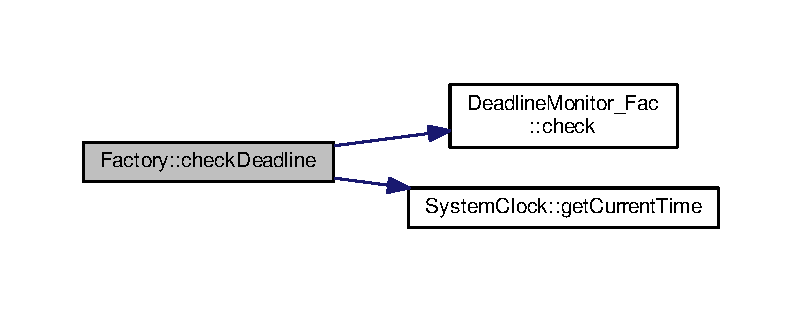
\includegraphics[width=350pt]{classFactory_a7f2a51ac39c034ccc0923eaa39cff780_cgraph}
\end{center}
\end{figure}


\index{Factory@{Factory}!exec\+Factory@{exec\+Factory}}
\index{exec\+Factory@{exec\+Factory}!Factory@{Factory}}
\subsubsection[{\texorpdfstring{exec\+Factory(std\+::vector$<$ char $\ast$ $>$ atomic\+\_\+list)}{execFactory(std::vector< char * > atomic_list)}}]{\setlength{\rightskip}{0pt plus 5cm}template$<$typename Data\+\_\+0 , typename Data\+\_\+1 , typename Data\+\_\+2 , typename Data\+\_\+3 , typename Data\+\_\+4 , typename Data\+\_\+5 , typename Data\+\_\+6 , typename Data\+\_\+7 , typename Data\+\_\+8 , typename Data\+\_\+9 $>$ void {\bf Factory}$<$ Data\+\_\+0, Data\+\_\+1, Data\+\_\+2, Data\+\_\+3, Data\+\_\+4, Data\+\_\+5, Data\+\_\+6, Data\+\_\+7, Data\+\_\+8, Data\+\_\+9 $>$\+::exec\+Factory (
\begin{DoxyParamCaption}
\item[{std\+::vector$<$ char $\ast$ $>$}]{atomic\+\_\+list}
\end{DoxyParamCaption}
)}\hypertarget{classFactory_aef23e931404b99e10ae4d9b8723e24a6}{}\label{classFactory_aef23e931404b99e10ae4d9b8723e24a6}


Factory\+\_\+old.\+cpp 파일의 487 번째 라인에서 정의되었습니다.



다음을 참조함 \+:  Factory$<$ Data\+\_\+0, Data\+\_\+1, Data\+\_\+2, Data\+\_\+3, Data\+\_\+4, Data\+\_\+5, Data\+\_\+6, Data\+\_\+7, Data\+\_\+8, Data\+\_\+9 $>$\+::connector\+\_\+iter\+\_\+1, Factory$<$ Data\+\_\+0, Data\+\_\+1, Data\+\_\+2, Data\+\_\+3, Data\+\_\+4, Data\+\_\+5, Data\+\_\+6, Data\+\_\+7, Data\+\_\+8, Data\+\_\+9 $>$\+::connector\+\_\+iter\+\_\+2, Factory$<$ Data\+\_\+0, Data\+\_\+1, Data\+\_\+2, Data\+\_\+3, Data\+\_\+4, Data\+\_\+5, Data\+\_\+6, Data\+\_\+7, Data\+\_\+8, Data\+\_\+9 $>$\+::connector\+\_\+iter\+\_\+3, Factory$<$ Data\+\_\+0, Data\+\_\+1, Data\+\_\+2, Data\+\_\+3, Data\+\_\+4, Data\+\_\+5, Data\+\_\+6, Data\+\_\+7, Data\+\_\+8, Data\+\_\+9 $>$\+::connector\+\_\+iter\+\_\+4, Factory$<$ Data\+\_\+0, Data\+\_\+1, Data\+\_\+2, Data\+\_\+3, Data\+\_\+4, Data\+\_\+5, Data\+\_\+6, Data\+\_\+7, Data\+\_\+8, Data\+\_\+9 $>$\+::connector\+\_\+iter\+\_\+5, Factory$<$ Data\+\_\+0, Data\+\_\+1, Data\+\_\+2, Data\+\_\+3, Data\+\_\+4, Data\+\_\+5, Data\+\_\+6, Data\+\_\+7, Data\+\_\+8, Data\+\_\+9 $>$\+::exec\+Factory\+Port\+\_\+in(), Factory$<$ Data\+\_\+0, Data\+\_\+1, Data\+\_\+2, Data\+\_\+3, Data\+\_\+4, Data\+\_\+5, Data\+\_\+6, Data\+\_\+7, Data\+\_\+8, Data\+\_\+9 $>$\+::exec\+Factory\+Port\+\_\+out(), Factory$<$ Data\+\_\+0, Data\+\_\+1, Data\+\_\+2, Data\+\_\+3, Data\+\_\+4, Data\+\_\+5, Data\+\_\+6, Data\+\_\+7, Data\+\_\+8, Data\+\_\+9 $>$\+::\+I\+D\+P0, Factory$<$ Data\+\_\+0, Data\+\_\+1, Data\+\_\+2, Data\+\_\+3, Data\+\_\+4, Data\+\_\+5, Data\+\_\+6, Data\+\_\+7, Data\+\_\+8, Data\+\_\+9 $>$\+::\+I\+D\+P1, Factory$<$ Data\+\_\+0, Data\+\_\+1, Data\+\_\+2, Data\+\_\+3, Data\+\_\+4, Data\+\_\+5, Data\+\_\+6, Data\+\_\+7, Data\+\_\+8, Data\+\_\+9 $>$\+::\+I\+D\+P2, Factory$<$ Data\+\_\+0, Data\+\_\+1, Data\+\_\+2, Data\+\_\+3, Data\+\_\+4, Data\+\_\+5, Data\+\_\+6, Data\+\_\+7, Data\+\_\+8, Data\+\_\+9 $>$\+::\+I\+D\+P3, Factory$<$ Data\+\_\+0, Data\+\_\+1, Data\+\_\+2, Data\+\_\+3, Data\+\_\+4, Data\+\_\+5, Data\+\_\+6, Data\+\_\+7, Data\+\_\+8, Data\+\_\+9 $>$\+::\+I\+D\+P4, Factory$<$ Data\+\_\+0, Data\+\_\+1, Data\+\_\+2, Data\+\_\+3, Data\+\_\+4, Data\+\_\+5, Data\+\_\+6, Data\+\_\+7, Data\+\_\+8, Data\+\_\+9 $>$\+::input\+\_\+data\+\_\+1, Factory$<$ Data\+\_\+0, Data\+\_\+1, Data\+\_\+2, Data\+\_\+3, Data\+\_\+4, Data\+\_\+5, Data\+\_\+6, Data\+\_\+7, Data\+\_\+8, Data\+\_\+9 $>$\+::input\+\_\+data\+\_\+2, Factory$<$ Data\+\_\+0, Data\+\_\+1, Data\+\_\+2, Data\+\_\+3, Data\+\_\+4, Data\+\_\+5, Data\+\_\+6, Data\+\_\+7, Data\+\_\+8, Data\+\_\+9 $>$\+::input\+\_\+data\+\_\+3, Factory$<$ Data\+\_\+0, Data\+\_\+1, Data\+\_\+2, Data\+\_\+3, Data\+\_\+4, Data\+\_\+5, Data\+\_\+6, Data\+\_\+7, Data\+\_\+8, Data\+\_\+9 $>$\+::input\+\_\+data\+\_\+4, Factory$<$ Data\+\_\+0, Data\+\_\+1, Data\+\_\+2, Data\+\_\+3, Data\+\_\+4, Data\+\_\+5, Data\+\_\+6, Data\+\_\+7, Data\+\_\+8, Data\+\_\+9 $>$\+::input\+\_\+data\+\_\+5, Factory$<$ Data\+\_\+0, Data\+\_\+1, Data\+\_\+2, Data\+\_\+3, Data\+\_\+4, Data\+\_\+5, Data\+\_\+6, Data\+\_\+7, Data\+\_\+8, Data\+\_\+9 $>$\+::iter\+\_\+1, Factory$<$ Data\+\_\+0, Data\+\_\+1, Data\+\_\+2, Data\+\_\+3, Data\+\_\+4, Data\+\_\+5, Data\+\_\+6, Data\+\_\+7, Data\+\_\+8, Data\+\_\+9 $>$\+::iter\+\_\+2, Factory$<$ Data\+\_\+0, Data\+\_\+1, Data\+\_\+2, Data\+\_\+3, Data\+\_\+4, Data\+\_\+5, Data\+\_\+6, Data\+\_\+7, Data\+\_\+8, Data\+\_\+9 $>$\+::iter\+\_\+3, Factory$<$ Data\+\_\+0, Data\+\_\+1, Data\+\_\+2, Data\+\_\+3, Data\+\_\+4, Data\+\_\+5, Data\+\_\+6, Data\+\_\+7, Data\+\_\+8, Data\+\_\+9 $>$\+::iter\+\_\+4, Factory$<$ Data\+\_\+0, Data\+\_\+1, Data\+\_\+2, Data\+\_\+3, Data\+\_\+4, Data\+\_\+5, Data\+\_\+6, Data\+\_\+7, Data\+\_\+8, Data\+\_\+9 $>$\+::iter\+\_\+5, Factory$<$ Data\+\_\+0, Data\+\_\+1, Data\+\_\+2, Data\+\_\+3, Data\+\_\+4, Data\+\_\+5, Data\+\_\+6, Data\+\_\+7, Data\+\_\+8, Data\+\_\+9 $>$\+::\+O\+D\+P0, Factory$<$ Data\+\_\+0, Data\+\_\+1, Data\+\_\+2, Data\+\_\+3, Data\+\_\+4, Data\+\_\+5, Data\+\_\+6, Data\+\_\+7, Data\+\_\+8, Data\+\_\+9 $>$\+::\+O\+D\+P1, Factory$<$ Data\+\_\+0, Data\+\_\+1, Data\+\_\+2, Data\+\_\+3, Data\+\_\+4, Data\+\_\+5, Data\+\_\+6, Data\+\_\+7, Data\+\_\+8, Data\+\_\+9 $>$\+::\+O\+D\+P2, Factory$<$ Data\+\_\+0, Data\+\_\+1, Data\+\_\+2, Data\+\_\+3, Data\+\_\+4, Data\+\_\+5, Data\+\_\+6, Data\+\_\+7, Data\+\_\+8, Data\+\_\+9 $>$\+::\+O\+D\+P3, Factory$<$ Data\+\_\+0, Data\+\_\+1, Data\+\_\+2, Data\+\_\+3, Data\+\_\+4, Data\+\_\+5, Data\+\_\+6, Data\+\_\+7, Data\+\_\+8, Data\+\_\+9 $>$\+::\+O\+D\+P4, Factory$<$ Data\+\_\+0, Data\+\_\+1, Data\+\_\+2, Data\+\_\+3, Data\+\_\+4, Data\+\_\+5, Data\+\_\+6, Data\+\_\+7, Data\+\_\+8, Data\+\_\+9 $>$\+::output\+\_\+connector\+\_\+data\+\_\+1, Factory$<$ Data\+\_\+0, Data\+\_\+1, Data\+\_\+2, Data\+\_\+3, Data\+\_\+4, Data\+\_\+5, Data\+\_\+6, Data\+\_\+7, Data\+\_\+8, Data\+\_\+9 $>$\+::output\+\_\+connector\+\_\+data\+\_\+2, Factory$<$ Data\+\_\+0, Data\+\_\+1, Data\+\_\+2, Data\+\_\+3, Data\+\_\+4, Data\+\_\+5, Data\+\_\+6, Data\+\_\+7, Data\+\_\+8, Data\+\_\+9 $>$\+::output\+\_\+connector\+\_\+data\+\_\+3, Factory$<$ Data\+\_\+0, Data\+\_\+1, Data\+\_\+2, Data\+\_\+3, Data\+\_\+4, Data\+\_\+5, Data\+\_\+6, Data\+\_\+7, Data\+\_\+8, Data\+\_\+9 $>$\+::output\+\_\+connector\+\_\+data\+\_\+4, Factory$<$ Data\+\_\+0, Data\+\_\+1, Data\+\_\+2, Data\+\_\+3, Data\+\_\+4, Data\+\_\+5, Data\+\_\+6, Data\+\_\+7, Data\+\_\+8, Data\+\_\+9 $>$\+::output\+\_\+connector\+\_\+data\+\_\+5.



이 함수 내부에서 호출하는 함수들에 대한 그래프입니다.\+:\nopagebreak
\begin{figure}[H]
\begin{center}
\leavevmode
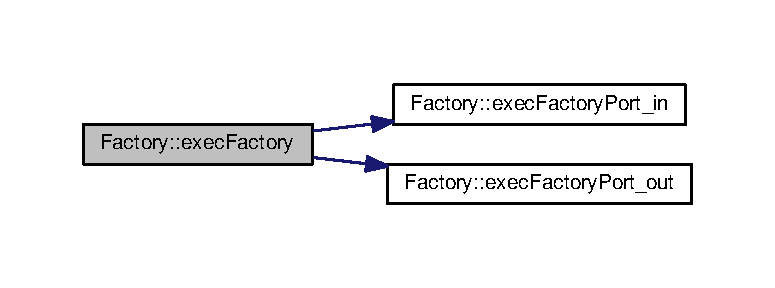
\includegraphics[width=350pt]{classFactory_aef23e931404b99e10ae4d9b8723e24a6_cgraph}
\end{center}
\end{figure}


\index{Factory@{Factory}!exec\+Factory@{exec\+Factory}}
\index{exec\+Factory@{exec\+Factory}!Factory@{Factory}}
\subsubsection[{\texorpdfstring{exec\+Factory(std\+::vector$<$ const char $\ast$ $>$ atomic\+\_\+list)}{execFactory(std::vector< const char * > atomic_list)}}]{\setlength{\rightskip}{0pt plus 5cm}template$<$typename Data\+\_\+0 , typename Data\+\_\+1 , typename Data\+\_\+2 , typename Data\+\_\+3 , typename Data\+\_\+4 , typename Data\+\_\+5 , typename Data\+\_\+6 , typename Data\+\_\+7 , typename Data\+\_\+8 , typename Data\+\_\+9 $>$ void {\bf Factory}$<$ Data\+\_\+0, Data\+\_\+1, Data\+\_\+2, Data\+\_\+3, Data\+\_\+4, Data\+\_\+5, Data\+\_\+6, Data\+\_\+7, Data\+\_\+8, Data\+\_\+9 $>$\+::exec\+Factory (
\begin{DoxyParamCaption}
\item[{std\+::vector$<$ const char $\ast$ $>$}]{atomic\+\_\+list}
\end{DoxyParamCaption}
)}\hypertarget{classFactory_a500058128cac41fd5fd45aac1a8f3d7d}{}\label{classFactory_a500058128cac41fd5fd45aac1a8f3d7d}


Factory.\+cpp 파일의 899 번째 라인에서 정의되었습니다.



다음에 의해서 참조됨 \+:  main().



이 함수를 호출하는 함수들에 대한 그래프입니다.\+:\nopagebreak
\begin{figure}[H]
\begin{center}
\leavevmode
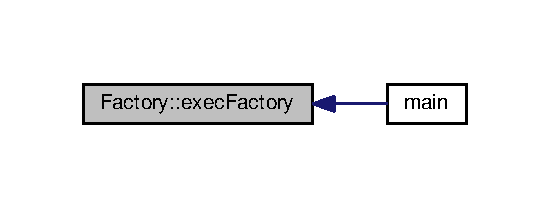
\includegraphics[width=264pt]{classFactory_a500058128cac41fd5fd45aac1a8f3d7d_icgraph}
\end{center}
\end{figure}


\index{Factory@{Factory}!exec\+Factory\+Port\+\_\+in@{exec\+Factory\+Port\+\_\+in}}
\index{exec\+Factory\+Port\+\_\+in@{exec\+Factory\+Port\+\_\+in}!Factory@{Factory}}
\subsubsection[{\texorpdfstring{exec\+Factory\+Port\+\_\+in()}{execFactoryPort_in()}}]{\setlength{\rightskip}{0pt plus 5cm}template$<$typename Data\+\_\+0, typename Data\+\_\+1, typename Data\+\_\+2, typename Data\+\_\+3, typename Data\+\_\+4, typename Data\+\_\+5, typename Data\+\_\+6, typename Data\+\_\+7, typename Data\+\_\+8, typename Data\+\_\+9$>$ void {\bf Factory}$<$ Data\+\_\+0, Data\+\_\+1, Data\+\_\+2, Data\+\_\+3, Data\+\_\+4, Data\+\_\+5, Data\+\_\+6, Data\+\_\+7, Data\+\_\+8, Data\+\_\+9 $>$\+::exec\+Factory\+Port\+\_\+in (
\begin{DoxyParamCaption}
{}
\end{DoxyParamCaption}
)}\hypertarget{classFactory_a6ffc6624a41ccd66f6ba05b696e50211}{}\label{classFactory_a6ffc6624a41ccd66f6ba05b696e50211}
\index{Factory@{Factory}!exec\+Factory\+Port\+\_\+in@{exec\+Factory\+Port\+\_\+in}}
\index{exec\+Factory\+Port\+\_\+in@{exec\+Factory\+Port\+\_\+in}!Factory@{Factory}}
\subsubsection[{\texorpdfstring{exec\+Factory\+Port\+\_\+in()}{execFactoryPort_in()}}]{\setlength{\rightskip}{0pt plus 5cm}template$<$typename Data\+\_\+0 , typename Data\+\_\+1 , typename Data\+\_\+2 , typename Data\+\_\+3 , typename Data\+\_\+4 , typename Data\+\_\+5 , typename Data\+\_\+6 , typename Data\+\_\+7 , typename Data\+\_\+8 , typename Data\+\_\+9 $>$ void {\bf Factory}$<$ Data\+\_\+0, Data\+\_\+1, Data\+\_\+2, Data\+\_\+3, Data\+\_\+4, Data\+\_\+5, Data\+\_\+6, Data\+\_\+7, Data\+\_\+8, Data\+\_\+9 $>$\+::exec\+Factory\+Port\+\_\+in (
\begin{DoxyParamCaption}
{}
\end{DoxyParamCaption}
)}\hypertarget{classFactory_a6ffc6624a41ccd66f6ba05b696e50211}{}\label{classFactory_a6ffc6624a41ccd66f6ba05b696e50211}


Factory.\+cpp 파일의 1251 번째 라인에서 정의되었습니다.



다음에 의해서 참조됨 \+:  Factory$<$ Data\+\_\+0, Data\+\_\+1, Data\+\_\+2, Data\+\_\+3, Data\+\_\+4, Data\+\_\+5, Data\+\_\+6, Data\+\_\+7, Data\+\_\+8, Data\+\_\+9 $>$\+::exec\+Factory().



이 함수를 호출하는 함수들에 대한 그래프입니다.\+:\nopagebreak
\begin{figure}[H]
\begin{center}
\leavevmode
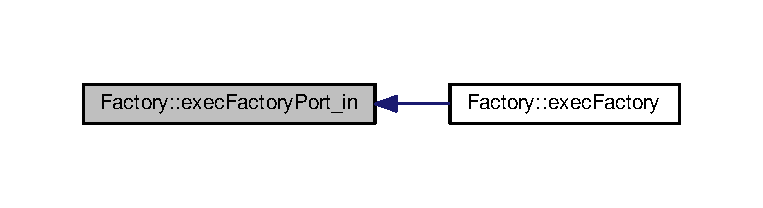
\includegraphics[width=350pt]{classFactory_a6ffc6624a41ccd66f6ba05b696e50211_icgraph}
\end{center}
\end{figure}


\index{Factory@{Factory}!exec\+Factory\+Port\+\_\+out@{exec\+Factory\+Port\+\_\+out}}
\index{exec\+Factory\+Port\+\_\+out@{exec\+Factory\+Port\+\_\+out}!Factory@{Factory}}
\subsubsection[{\texorpdfstring{exec\+Factory\+Port\+\_\+out()}{execFactoryPort_out()}}]{\setlength{\rightskip}{0pt plus 5cm}template$<$typename Data\+\_\+0, typename Data\+\_\+1, typename Data\+\_\+2, typename Data\+\_\+3, typename Data\+\_\+4, typename Data\+\_\+5, typename Data\+\_\+6, typename Data\+\_\+7, typename Data\+\_\+8, typename Data\+\_\+9$>$ void {\bf Factory}$<$ Data\+\_\+0, Data\+\_\+1, Data\+\_\+2, Data\+\_\+3, Data\+\_\+4, Data\+\_\+5, Data\+\_\+6, Data\+\_\+7, Data\+\_\+8, Data\+\_\+9 $>$\+::exec\+Factory\+Port\+\_\+out (
\begin{DoxyParamCaption}
{}
\end{DoxyParamCaption}
)}\hypertarget{classFactory_a26be38da40eb21a04b0b4712282518e9}{}\label{classFactory_a26be38da40eb21a04b0b4712282518e9}
\index{Factory@{Factory}!exec\+Factory\+Port\+\_\+out@{exec\+Factory\+Port\+\_\+out}}
\index{exec\+Factory\+Port\+\_\+out@{exec\+Factory\+Port\+\_\+out}!Factory@{Factory}}
\subsubsection[{\texorpdfstring{exec\+Factory\+Port\+\_\+out()}{execFactoryPort_out()}}]{\setlength{\rightskip}{0pt plus 5cm}template$<$typename Data\+\_\+0 , typename Data\+\_\+1 , typename Data\+\_\+2 , typename Data\+\_\+3 , typename Data\+\_\+4 , typename Data\+\_\+5 , typename Data\+\_\+6 , typename Data\+\_\+7 , typename Data\+\_\+8 , typename Data\+\_\+9 $>$ void {\bf Factory}$<$ Data\+\_\+0, Data\+\_\+1, Data\+\_\+2, Data\+\_\+3, Data\+\_\+4, Data\+\_\+5, Data\+\_\+6, Data\+\_\+7, Data\+\_\+8, Data\+\_\+9 $>$\+::exec\+Factory\+Port\+\_\+out (
\begin{DoxyParamCaption}
{}
\end{DoxyParamCaption}
)}\hypertarget{classFactory_a26be38da40eb21a04b0b4712282518e9}{}\label{classFactory_a26be38da40eb21a04b0b4712282518e9}


Factory.\+cpp 파일의 1277 번째 라인에서 정의되었습니다.



다음에 의해서 참조됨 \+:  Factory$<$ Data\+\_\+0, Data\+\_\+1, Data\+\_\+2, Data\+\_\+3, Data\+\_\+4, Data\+\_\+5, Data\+\_\+6, Data\+\_\+7, Data\+\_\+8, Data\+\_\+9 $>$\+::exec\+Factory(), main().



이 함수를 호출하는 함수들에 대한 그래프입니다.\+:\nopagebreak
\begin{figure}[H]
\begin{center}
\leavevmode
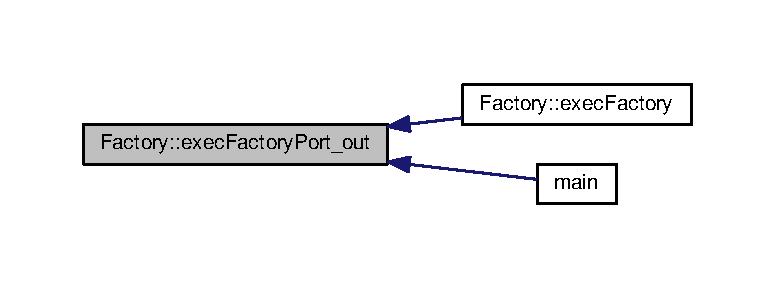
\includegraphics[width=350pt]{classFactory_a26be38da40eb21a04b0b4712282518e9_icgraph}
\end{center}
\end{figure}


\index{Factory@{Factory}!F\+I\+P\+\_\+create@{F\+I\+P\+\_\+create}}
\index{F\+I\+P\+\_\+create@{F\+I\+P\+\_\+create}!Factory@{Factory}}
\subsubsection[{\texorpdfstring{F\+I\+P\+\_\+create(const int port\+\_\+id)}{FIP_create(const int port_id)}}]{\setlength{\rightskip}{0pt plus 5cm}template$<$typename Data\+\_\+0 , typename Data\+\_\+1 , typename Data\+\_\+2 , typename Data\+\_\+3 , typename Data\+\_\+4 , typename Data\+\_\+5 , typename Data\+\_\+6 , typename Data\+\_\+7 , typename Data\+\_\+8 , typename Data\+\_\+9 $>$ void {\bf Factory}$<$ Data\+\_\+0, Data\+\_\+1, Data\+\_\+2, Data\+\_\+3, Data\+\_\+4, Data\+\_\+5, Data\+\_\+6, Data\+\_\+7, Data\+\_\+8, Data\+\_\+9 $>$\+::F\+I\+P\+\_\+create (
\begin{DoxyParamCaption}
\item[{const int}]{port\+\_\+id}
\end{DoxyParamCaption}
)}\hypertarget{classFactory_a83757b0ec4d4c3f1e6c1df0cbca2a5d9}{}\label{classFactory_a83757b0ec4d4c3f1e6c1df0cbca2a5d9}


Factory.\+cpp 파일의 920 번째 라인에서 정의되었습니다.

\index{Factory@{Factory}!F\+O\+P\+\_\+create@{F\+O\+P\+\_\+create}}
\index{F\+O\+P\+\_\+create@{F\+O\+P\+\_\+create}!Factory@{Factory}}
\subsubsection[{\texorpdfstring{F\+O\+P\+\_\+create(const int port\+\_\+id)}{FOP_create(const int port_id)}}]{\setlength{\rightskip}{0pt plus 5cm}template$<$typename Data\+\_\+0 , typename Data\+\_\+1 , typename Data\+\_\+2 , typename Data\+\_\+3 , typename Data\+\_\+4 , typename Data\+\_\+5 , typename Data\+\_\+6 , typename Data\+\_\+7 , typename Data\+\_\+8 , typename Data\+\_\+9 $>$ void {\bf Factory}$<$ Data\+\_\+0, Data\+\_\+1, Data\+\_\+2, Data\+\_\+3, Data\+\_\+4, Data\+\_\+5, Data\+\_\+6, Data\+\_\+7, Data\+\_\+8, Data\+\_\+9 $>$\+::F\+O\+P\+\_\+create (
\begin{DoxyParamCaption}
\item[{const int}]{port\+\_\+id}
\end{DoxyParamCaption}
)}\hypertarget{classFactory_a37a09c78d3bf8fb3df5ece85bace2733}{}\label{classFactory_a37a09c78d3bf8fb3df5ece85bace2733}


Factory.\+cpp 파일의 1088 번째 라인에서 정의되었습니다.



다음을 참조함 \+:  System\+Clock\+::get\+Current\+Time().



이 함수 내부에서 호출하는 함수들에 대한 그래프입니다.\+:\nopagebreak
\begin{figure}[H]
\begin{center}
\leavevmode
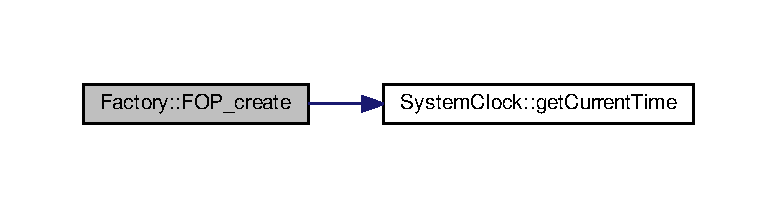
\includegraphics[width=350pt]{classFactory_a37a09c78d3bf8fb3df5ece85bace2733_cgraph}
\end{center}
\end{figure}


\index{Factory@{Factory}!initialize@{initialize}}
\index{initialize@{initialize}!Factory@{Factory}}
\subsubsection[{\texorpdfstring{initialize(std\+::string, double, int, int)}{initialize(std::string, double, int, int)}}]{\setlength{\rightskip}{0pt plus 5cm}template$<$typename Data\+\_\+0 , typename Data\+\_\+1 , typename Data\+\_\+2 , typename Data\+\_\+3 , typename Data\+\_\+4 , typename Data\+\_\+5 , typename Data\+\_\+6 , typename Data\+\_\+7 , typename Data\+\_\+8 , typename Data\+\_\+9 $>$ void {\bf Factory}$<$ Data\+\_\+0, Data\+\_\+1, Data\+\_\+2, Data\+\_\+3, Data\+\_\+4, Data\+\_\+5, Data\+\_\+6, Data\+\_\+7, Data\+\_\+8, Data\+\_\+9 $>$\+::initialize (
\begin{DoxyParamCaption}
\item[{std\+::string}]{name, }
\item[{double}]{deadline, }
\item[{int}]{node\+\_\+id, }
\item[{int}]{core\+\_\+id}
\end{DoxyParamCaption}
)}\hypertarget{classFactory_af9ced939952de12016774d0225c93520}{}\label{classFactory_af9ced939952de12016774d0225c93520}


Factory\+\_\+old.\+cpp 파일의 729 번째 라인에서 정의되었습니다.

\index{Factory@{Factory}!initialize@{initialize}}
\index{initialize@{initialize}!Factory@{Factory}}
\subsubsection[{\texorpdfstring{initialize(std\+::string name, int64\+\_\+t deadline, void($\ast$deadline\+\_\+handler)(), int node\+\_\+id, int core\+\_\+id)}{initialize(std::string name, int64_t deadline, void(*deadline_handler)(), int node_id, int core_id)}}]{\setlength{\rightskip}{0pt plus 5cm}template$<$typename Data\+\_\+0 , typename Data\+\_\+1 , typename Data\+\_\+2 , typename Data\+\_\+3 , typename Data\+\_\+4 , typename Data\+\_\+5 , typename Data\+\_\+6 , typename Data\+\_\+7 , typename Data\+\_\+8 , typename Data\+\_\+9 $>$ void {\bf Factory}$<$ Data\+\_\+0, Data\+\_\+1, Data\+\_\+2, Data\+\_\+3, Data\+\_\+4, Data\+\_\+5, Data\+\_\+6, Data\+\_\+7, Data\+\_\+8, Data\+\_\+9 $>$\+::initialize (
\begin{DoxyParamCaption}
\item[{std\+::string}]{name, }
\item[{int64\+\_\+t}]{deadline, }
\item[{void($\ast$)()}]{deadline\+\_\+handler, }
\item[{int}]{node\+\_\+id, }
\item[{int}]{core\+\_\+id}
\end{DoxyParamCaption}
)}\hypertarget{classFactory_a64a97c299b156747868846be05ad9257}{}\label{classFactory_a64a97c299b156747868846be05ad9257}


Factory.\+cpp 파일의 1305 번째 라인에서 정의되었습니다.



다음을 참조함 \+:  deadline\+\_\+handler().



다음에 의해서 참조됨 \+:  Input\+Data\+Port\+\_\+\+Fac$<$ Data\+\_\+0, Data\+\_\+1, Data\+\_\+2, Data\+\_\+3, Data\+\_\+4, Data\+\_\+5, Data\+\_\+6, Data\+\_\+7, Data\+\_\+8, Data\+\_\+9 $>$\+::initialize(), main().



이 함수 내부에서 호출하는 함수들에 대한 그래프입니다.\+:\nopagebreak
\begin{figure}[H]
\begin{center}
\leavevmode
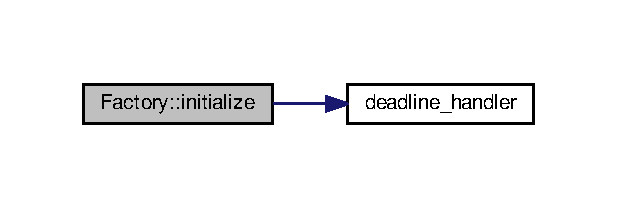
\includegraphics[width=296pt]{classFactory_a64a97c299b156747868846be05ad9257_cgraph}
\end{center}
\end{figure}




이 함수를 호출하는 함수들에 대한 그래프입니다.\+:\nopagebreak
\begin{figure}[H]
\begin{center}
\leavevmode
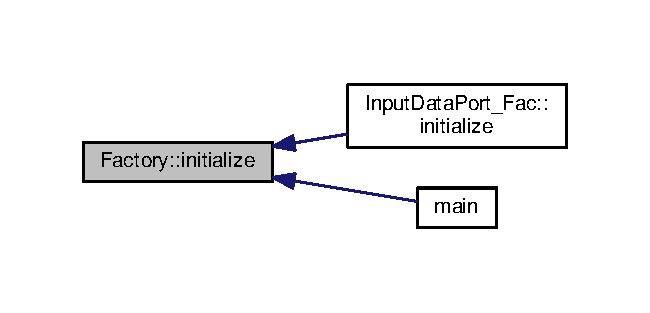
\includegraphics[width=312pt]{classFactory_a64a97c299b156747868846be05ad9257_icgraph}
\end{center}
\end{figure}


\index{Factory@{Factory}!set\+Deadline@{set\+Deadline}}
\index{set\+Deadline@{set\+Deadline}!Factory@{Factory}}
\subsubsection[{\texorpdfstring{set\+Deadline(int64\+\_\+t deadline, void($\ast$deadline\+\_\+handler)())}{setDeadline(int64_t deadline, void(*deadline_handler)())}}]{\setlength{\rightskip}{0pt plus 5cm}template$<$typename Data\+\_\+0 , typename Data\+\_\+1 , typename Data\+\_\+2 , typename Data\+\_\+3 , typename Data\+\_\+4 , typename Data\+\_\+5 , typename Data\+\_\+6 , typename Data\+\_\+7 , typename Data\+\_\+8 , typename Data\+\_\+9 $>$ void {\bf Factory}$<$ Data\+\_\+0, Data\+\_\+1, Data\+\_\+2, Data\+\_\+3, Data\+\_\+4, Data\+\_\+5, Data\+\_\+6, Data\+\_\+7, Data\+\_\+8, Data\+\_\+9 $>$\+::set\+Deadline (
\begin{DoxyParamCaption}
\item[{int64\+\_\+t}]{deadline, }
\item[{void($\ast$)()}]{deadline\+\_\+handler}
\end{DoxyParamCaption}
)}\hypertarget{classFactory_ab884eec61738ee5f0fcf7d25a4855bc0}{}\label{classFactory_ab884eec61738ee5f0fcf7d25a4855bc0}


Factory.\+cpp 파일의 280 번째 라인에서 정의되었습니다.



다음을 참조함 \+:  deadline\+\_\+handler(), Deadline\+Monitor\+\_\+\+Fac\+::setup().



이 함수 내부에서 호출하는 함수들에 대한 그래프입니다.\+:\nopagebreak
\begin{figure}[H]
\begin{center}
\leavevmode
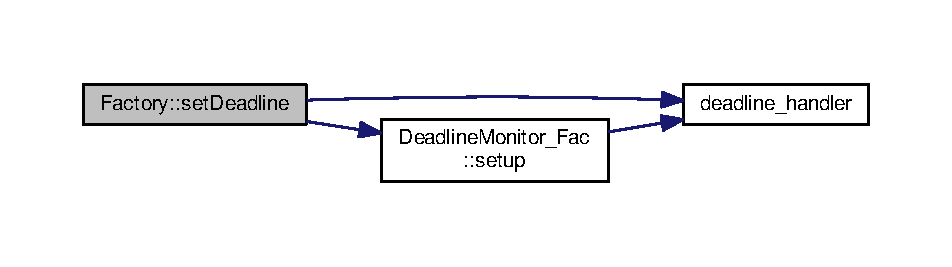
\includegraphics[width=350pt]{classFactory_ab884eec61738ee5f0fcf7d25a4855bc0_cgraph}
\end{center}
\end{figure}


\index{Factory@{Factory}!update\+Deadline\+F\+IP@{update\+Deadline\+F\+IP}}
\index{update\+Deadline\+F\+IP@{update\+Deadline\+F\+IP}!Factory@{Factory}}
\subsubsection[{\texorpdfstring{update\+Deadline\+F\+I\+P(int64\+\_\+t $\ast$msg\+\_\+duetime)}{updateDeadlineFIP(int64_t *msg_duetime)}}]{\setlength{\rightskip}{0pt plus 5cm}template$<$typename Data\+\_\+0 , typename Data\+\_\+1 , typename Data\+\_\+2 , typename Data\+\_\+3 , typename Data\+\_\+4 , typename Data\+\_\+5 , typename Data\+\_\+6 , typename Data\+\_\+7 , typename Data\+\_\+8 , typename Data\+\_\+9 $>$ void {\bf Factory}$<$ Data\+\_\+0, Data\+\_\+1, Data\+\_\+2, Data\+\_\+3, Data\+\_\+4, Data\+\_\+5, Data\+\_\+6, Data\+\_\+7, Data\+\_\+8, Data\+\_\+9 $>$\+::update\+Deadline\+F\+IP (
\begin{DoxyParamCaption}
\item[{int64\+\_\+t $\ast$}]{msg\+\_\+duetime}
\end{DoxyParamCaption}
)}\hypertarget{classFactory_a5982eaac979b3ef080244ddc5007b690}{}\label{classFactory_a5982eaac979b3ef080244ddc5007b690}


Factory.\+cpp 파일의 259 번째 라인에서 정의되었습니다.



다음을 참조함 \+:  Deadline\+Monitor\+\_\+\+Fac\+::update().



이 함수 내부에서 호출하는 함수들에 대한 그래프입니다.\+:\nopagebreak
\begin{figure}[H]
\begin{center}
\leavevmode
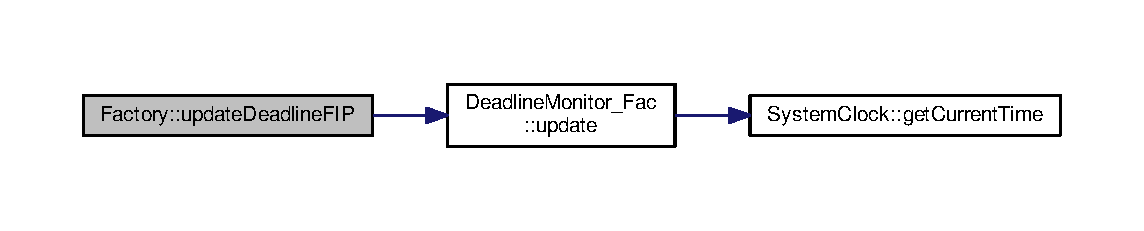
\includegraphics[width=350pt]{classFactory_a5982eaac979b3ef080244ddc5007b690_cgraph}
\end{center}
\end{figure}


\index{Factory@{Factory}!update\+Deadline\+F\+OP@{update\+Deadline\+F\+OP}}
\index{update\+Deadline\+F\+OP@{update\+Deadline\+F\+OP}!Factory@{Factory}}
\subsubsection[{\texorpdfstring{update\+Deadline\+F\+O\+P(int64\+\_\+t $\ast$msg\+\_\+duetime)}{updateDeadlineFOP(int64_t *msg_duetime)}}]{\setlength{\rightskip}{0pt plus 5cm}template$<$typename Data\+\_\+0 , typename Data\+\_\+1 , typename Data\+\_\+2 , typename Data\+\_\+3 , typename Data\+\_\+4 , typename Data\+\_\+5 , typename Data\+\_\+6 , typename Data\+\_\+7 , typename Data\+\_\+8 , typename Data\+\_\+9 $>$ void {\bf Factory}$<$ Data\+\_\+0, Data\+\_\+1, Data\+\_\+2, Data\+\_\+3, Data\+\_\+4, Data\+\_\+5, Data\+\_\+6, Data\+\_\+7, Data\+\_\+8, Data\+\_\+9 $>$\+::update\+Deadline\+F\+OP (
\begin{DoxyParamCaption}
\item[{int64\+\_\+t $\ast$}]{msg\+\_\+duetime}
\end{DoxyParamCaption}
)}\hypertarget{classFactory_a0777c31e360f6c08f9069482501e3a70}{}\label{classFactory_a0777c31e360f6c08f9069482501e3a70}


Factory.\+cpp 파일의 270 번째 라인에서 정의되었습니다.



\subsection{멤버 데이타 문서화}
\index{Factory@{Factory}!\+\_\+deadline\+\_\+monitor@{\+\_\+deadline\+\_\+monitor}}
\index{\+\_\+deadline\+\_\+monitor@{\+\_\+deadline\+\_\+monitor}!Factory@{Factory}}
\subsubsection[{\texorpdfstring{\+\_\+deadline\+\_\+monitor}{_deadline_monitor}}]{\setlength{\rightskip}{0pt plus 5cm}template$<$typename Data\+\_\+0, typename Data\+\_\+1, typename Data\+\_\+2, typename Data\+\_\+3, typename Data\+\_\+4, typename Data\+\_\+5, typename Data\+\_\+6, typename Data\+\_\+7, typename Data\+\_\+8, typename Data\+\_\+9$>$ {\bf Deadline\+Monitor\+\_\+\+Fac} {\bf Factory}$<$ Data\+\_\+0, Data\+\_\+1, Data\+\_\+2, Data\+\_\+3, Data\+\_\+4, Data\+\_\+5, Data\+\_\+6, Data\+\_\+7, Data\+\_\+8, Data\+\_\+9 $>$\+::\+\_\+deadline\+\_\+monitor\hspace{0.3cm}{\ttfamily [private]}}\hypertarget{classFactory_a4297ef21a23413ade2d0a528582c9946}{}\label{classFactory_a4297ef21a23413ade2d0a528582c9946}


Factory.\+cpp 파일의 100 번째 라인에서 정의되었습니다.

\index{Factory@{Factory}!connected\+\_\+ports@{connected\+\_\+ports}}
\index{connected\+\_\+ports@{connected\+\_\+ports}!Factory@{Factory}}
\subsubsection[{\texorpdfstring{connected\+\_\+ports}{connected_ports}}]{\setlength{\rightskip}{0pt plus 5cm}template$<$typename Data\+\_\+0, typename Data\+\_\+1, typename Data\+\_\+2, typename Data\+\_\+3, typename Data\+\_\+4, typename Data\+\_\+5, typename Data\+\_\+6, typename Data\+\_\+7, typename Data\+\_\+8, typename Data\+\_\+9$>$ std\+::bitset$<$ 10 $>$ {\bf Factory}$<$ Data\+\_\+0, Data\+\_\+1, Data\+\_\+2, Data\+\_\+3, Data\+\_\+4, Data\+\_\+5, Data\+\_\+6, Data\+\_\+7, Data\+\_\+8, Data\+\_\+9 $>$\+::connected\+\_\+ports}\hypertarget{classFactory_a47d1a95acef574eae4410faf891130df}{}\label{classFactory_a47d1a95acef574eae4410faf891130df}


Factory.\+cpp 파일의 115 번째 라인에서 정의되었습니다.



다음에 의해서 참조됨 \+:  Input\+Data\+Port\+\_\+\+Fac$<$ Data\+\_\+0, Data\+\_\+1, Data\+\_\+2, Data\+\_\+3, Data\+\_\+4, Data\+\_\+5, Data\+\_\+6, Data\+\_\+7, Data\+\_\+8, Data\+\_\+9 $>$\+::attach(), Output\+Data\+Port\+\_\+\+Fac$<$ Data\+\_\+0, Data\+\_\+1, Data\+\_\+2, Data\+\_\+3, Data\+\_\+4, Data\+\_\+5, Data\+\_\+6, Data\+\_\+7, Data\+\_\+8, Data\+\_\+9 $>$\+::attach(), Input\+Data\+Port\+\_\+\+Fac$<$ Data\+\_\+0, Data\+\_\+1, Data\+\_\+2, Data\+\_\+3, Data\+\_\+4, Data\+\_\+5, Data\+\_\+6, Data\+\_\+7, Data\+\_\+8, Data\+\_\+9 $>$\+::initialize().

\index{Factory@{Factory}!connector\+\_\+iter\+\_\+1@{connector\+\_\+iter\+\_\+1}}
\index{connector\+\_\+iter\+\_\+1@{connector\+\_\+iter\+\_\+1}!Factory@{Factory}}
\subsubsection[{\texorpdfstring{connector\+\_\+iter\+\_\+1}{connector_iter_1}}]{\setlength{\rightskip}{0pt plus 5cm}template$<$typename Data\+\_\+0, typename Data\+\_\+1, typename Data\+\_\+2, typename Data\+\_\+3, typename Data\+\_\+4, typename Data\+\_\+5, typename Data\+\_\+6, typename Data\+\_\+7, typename Data\+\_\+8, typename Data\+\_\+9$>$ std\+::vector$<$ dds\+::sub\+::\+Sample$<$ Data\+\_\+5 $>$ $>$\+::iterator {\bf Factory}$<$ Data\+\_\+0, Data\+\_\+1, Data\+\_\+2, Data\+\_\+3, Data\+\_\+4, Data\+\_\+5, Data\+\_\+6, Data\+\_\+7, Data\+\_\+8, Data\+\_\+9 $>$\+::connector\+\_\+iter\+\_\+1}\hypertarget{classFactory_a560460eae381287c085b613c5330dadd}{}\label{classFactory_a560460eae381287c085b613c5330dadd}


Factory.\+cpp 파일의 151 번째 라인에서 정의되었습니다.



다음에 의해서 참조됨 \+:  Factory$<$ Data\+\_\+0, Data\+\_\+1, Data\+\_\+2, Data\+\_\+3, Data\+\_\+4, Data\+\_\+5, Data\+\_\+6, Data\+\_\+7, Data\+\_\+8, Data\+\_\+9 $>$\+::exec\+Factory().

\index{Factory@{Factory}!connector\+\_\+iter\+\_\+2@{connector\+\_\+iter\+\_\+2}}
\index{connector\+\_\+iter\+\_\+2@{connector\+\_\+iter\+\_\+2}!Factory@{Factory}}
\subsubsection[{\texorpdfstring{connector\+\_\+iter\+\_\+2}{connector_iter_2}}]{\setlength{\rightskip}{0pt plus 5cm}template$<$typename Data\+\_\+0, typename Data\+\_\+1, typename Data\+\_\+2, typename Data\+\_\+3, typename Data\+\_\+4, typename Data\+\_\+5, typename Data\+\_\+6, typename Data\+\_\+7, typename Data\+\_\+8, typename Data\+\_\+9$>$ std\+::vector$<$ dds\+::sub\+::\+Sample$<$ Data\+\_\+6 $>$ $>$\+::iterator {\bf Factory}$<$ Data\+\_\+0, Data\+\_\+1, Data\+\_\+2, Data\+\_\+3, Data\+\_\+4, Data\+\_\+5, Data\+\_\+6, Data\+\_\+7, Data\+\_\+8, Data\+\_\+9 $>$\+::connector\+\_\+iter\+\_\+2}\hypertarget{classFactory_acb10615bebab1e5eda677a8b41c0fd29}{}\label{classFactory_acb10615bebab1e5eda677a8b41c0fd29}


Factory.\+cpp 파일의 153 번째 라인에서 정의되었습니다.



다음에 의해서 참조됨 \+:  Factory$<$ Data\+\_\+0, Data\+\_\+1, Data\+\_\+2, Data\+\_\+3, Data\+\_\+4, Data\+\_\+5, Data\+\_\+6, Data\+\_\+7, Data\+\_\+8, Data\+\_\+9 $>$\+::exec\+Factory().

\index{Factory@{Factory}!connector\+\_\+iter\+\_\+3@{connector\+\_\+iter\+\_\+3}}
\index{connector\+\_\+iter\+\_\+3@{connector\+\_\+iter\+\_\+3}!Factory@{Factory}}
\subsubsection[{\texorpdfstring{connector\+\_\+iter\+\_\+3}{connector_iter_3}}]{\setlength{\rightskip}{0pt plus 5cm}template$<$typename Data\+\_\+0, typename Data\+\_\+1, typename Data\+\_\+2, typename Data\+\_\+3, typename Data\+\_\+4, typename Data\+\_\+5, typename Data\+\_\+6, typename Data\+\_\+7, typename Data\+\_\+8, typename Data\+\_\+9$>$ std\+::vector$<$ dds\+::sub\+::\+Sample$<$ Data\+\_\+7 $>$ $>$\+::iterator {\bf Factory}$<$ Data\+\_\+0, Data\+\_\+1, Data\+\_\+2, Data\+\_\+3, Data\+\_\+4, Data\+\_\+5, Data\+\_\+6, Data\+\_\+7, Data\+\_\+8, Data\+\_\+9 $>$\+::connector\+\_\+iter\+\_\+3}\hypertarget{classFactory_abe759623a3ab82ecd6ae3923629c397d}{}\label{classFactory_abe759623a3ab82ecd6ae3923629c397d}


Factory.\+cpp 파일의 155 번째 라인에서 정의되었습니다.



다음에 의해서 참조됨 \+:  Factory$<$ Data\+\_\+0, Data\+\_\+1, Data\+\_\+2, Data\+\_\+3, Data\+\_\+4, Data\+\_\+5, Data\+\_\+6, Data\+\_\+7, Data\+\_\+8, Data\+\_\+9 $>$\+::exec\+Factory().

\index{Factory@{Factory}!connector\+\_\+iter\+\_\+4@{connector\+\_\+iter\+\_\+4}}
\index{connector\+\_\+iter\+\_\+4@{connector\+\_\+iter\+\_\+4}!Factory@{Factory}}
\subsubsection[{\texorpdfstring{connector\+\_\+iter\+\_\+4}{connector_iter_4}}]{\setlength{\rightskip}{0pt plus 5cm}template$<$typename Data\+\_\+0, typename Data\+\_\+1, typename Data\+\_\+2, typename Data\+\_\+3, typename Data\+\_\+4, typename Data\+\_\+5, typename Data\+\_\+6, typename Data\+\_\+7, typename Data\+\_\+8, typename Data\+\_\+9$>$ std\+::vector$<$ dds\+::sub\+::\+Sample$<$ Data\+\_\+8 $>$ $>$\+::iterator {\bf Factory}$<$ Data\+\_\+0, Data\+\_\+1, Data\+\_\+2, Data\+\_\+3, Data\+\_\+4, Data\+\_\+5, Data\+\_\+6, Data\+\_\+7, Data\+\_\+8, Data\+\_\+9 $>$\+::connector\+\_\+iter\+\_\+4}\hypertarget{classFactory_aa664c801aed2472266996c3e3256c406}{}\label{classFactory_aa664c801aed2472266996c3e3256c406}


Factory.\+cpp 파일의 157 번째 라인에서 정의되었습니다.



다음에 의해서 참조됨 \+:  Factory$<$ Data\+\_\+0, Data\+\_\+1, Data\+\_\+2, Data\+\_\+3, Data\+\_\+4, Data\+\_\+5, Data\+\_\+6, Data\+\_\+7, Data\+\_\+8, Data\+\_\+9 $>$\+::exec\+Factory().

\index{Factory@{Factory}!connector\+\_\+iter\+\_\+5@{connector\+\_\+iter\+\_\+5}}
\index{connector\+\_\+iter\+\_\+5@{connector\+\_\+iter\+\_\+5}!Factory@{Factory}}
\subsubsection[{\texorpdfstring{connector\+\_\+iter\+\_\+5}{connector_iter_5}}]{\setlength{\rightskip}{0pt plus 5cm}template$<$typename Data\+\_\+0, typename Data\+\_\+1, typename Data\+\_\+2, typename Data\+\_\+3, typename Data\+\_\+4, typename Data\+\_\+5, typename Data\+\_\+6, typename Data\+\_\+7, typename Data\+\_\+8, typename Data\+\_\+9$>$ std\+::vector$<$ dds\+::sub\+::\+Sample$<$ Data\+\_\+9 $>$ $>$\+::iterator {\bf Factory}$<$ Data\+\_\+0, Data\+\_\+1, Data\+\_\+2, Data\+\_\+3, Data\+\_\+4, Data\+\_\+5, Data\+\_\+6, Data\+\_\+7, Data\+\_\+8, Data\+\_\+9 $>$\+::connector\+\_\+iter\+\_\+5}\hypertarget{classFactory_addefc1a08fde4845b9d68bd9c0743f94}{}\label{classFactory_addefc1a08fde4845b9d68bd9c0743f94}


Factory.\+cpp 파일의 159 번째 라인에서 정의되었습니다.



다음에 의해서 참조됨 \+:  Factory$<$ Data\+\_\+0, Data\+\_\+1, Data\+\_\+2, Data\+\_\+3, Data\+\_\+4, Data\+\_\+5, Data\+\_\+6, Data\+\_\+7, Data\+\_\+8, Data\+\_\+9 $>$\+::exec\+Factory().

\index{Factory@{Factory}!connector\+\_\+topic0@{connector\+\_\+topic0}}
\index{connector\+\_\+topic0@{connector\+\_\+topic0}!Factory@{Factory}}
\subsubsection[{\texorpdfstring{connector\+\_\+topic0}{connector_topic0}}]{\setlength{\rightskip}{0pt plus 5cm}template$<$typename Data\+\_\+0, typename Data\+\_\+1, typename Data\+\_\+2, typename Data\+\_\+3, typename Data\+\_\+4, typename Data\+\_\+5, typename Data\+\_\+6, typename Data\+\_\+7, typename Data\+\_\+8, typename Data\+\_\+9$>$ dds\+::topic\+::\+Topic$<$ Data\+\_\+0 $>$ $\ast$ {\bf Factory}$<$ Data\+\_\+0, Data\+\_\+1, Data\+\_\+2, Data\+\_\+3, Data\+\_\+4, Data\+\_\+5, Data\+\_\+6, Data\+\_\+7, Data\+\_\+8, Data\+\_\+9 $>$\+::connector\+\_\+topic0}\hypertarget{classFactory_a292d6100f4cee20be6f5f7b5f1ed13b5}{}\label{classFactory_a292d6100f4cee20be6f5f7b5f1ed13b5}


Factory.\+cpp 파일의 128 번째 라인에서 정의되었습니다.



다음에 의해서 참조됨 \+:  Input\+Data\+Port\+\_\+\+Fac$<$ Data\+\_\+0, Data\+\_\+1, Data\+\_\+2, Data\+\_\+3, Data\+\_\+4, Data\+\_\+5, Data\+\_\+6, Data\+\_\+7, Data\+\_\+8, Data\+\_\+9 $>$\+::attach().

\index{Factory@{Factory}!connector\+\_\+topic1@{connector\+\_\+topic1}}
\index{connector\+\_\+topic1@{connector\+\_\+topic1}!Factory@{Factory}}
\subsubsection[{\texorpdfstring{connector\+\_\+topic1}{connector_topic1}}]{\setlength{\rightskip}{0pt plus 5cm}template$<$typename Data\+\_\+0, typename Data\+\_\+1, typename Data\+\_\+2, typename Data\+\_\+3, typename Data\+\_\+4, typename Data\+\_\+5, typename Data\+\_\+6, typename Data\+\_\+7, typename Data\+\_\+8, typename Data\+\_\+9$>$ dds\+::topic\+::\+Topic$<$ Data\+\_\+1 $>$ $\ast$ {\bf Factory}$<$ Data\+\_\+0, Data\+\_\+1, Data\+\_\+2, Data\+\_\+3, Data\+\_\+4, Data\+\_\+5, Data\+\_\+6, Data\+\_\+7, Data\+\_\+8, Data\+\_\+9 $>$\+::connector\+\_\+topic1}\hypertarget{classFactory_a744afdb2e49dc636774fdd4a2f6ec2d1}{}\label{classFactory_a744afdb2e49dc636774fdd4a2f6ec2d1}


Factory.\+cpp 파일의 129 번째 라인에서 정의되었습니다.



다음에 의해서 참조됨 \+:  Input\+Data\+Port\+\_\+\+Fac$<$ Data\+\_\+0, Data\+\_\+1, Data\+\_\+2, Data\+\_\+3, Data\+\_\+4, Data\+\_\+5, Data\+\_\+6, Data\+\_\+7, Data\+\_\+8, Data\+\_\+9 $>$\+::attach().

\index{Factory@{Factory}!connector\+\_\+topic2@{connector\+\_\+topic2}}
\index{connector\+\_\+topic2@{connector\+\_\+topic2}!Factory@{Factory}}
\subsubsection[{\texorpdfstring{connector\+\_\+topic2}{connector_topic2}}]{\setlength{\rightskip}{0pt plus 5cm}template$<$typename Data\+\_\+0, typename Data\+\_\+1, typename Data\+\_\+2, typename Data\+\_\+3, typename Data\+\_\+4, typename Data\+\_\+5, typename Data\+\_\+6, typename Data\+\_\+7, typename Data\+\_\+8, typename Data\+\_\+9$>$ dds\+::topic\+::\+Topic$<$ Data\+\_\+2 $>$ $\ast$ {\bf Factory}$<$ Data\+\_\+0, Data\+\_\+1, Data\+\_\+2, Data\+\_\+3, Data\+\_\+4, Data\+\_\+5, Data\+\_\+6, Data\+\_\+7, Data\+\_\+8, Data\+\_\+9 $>$\+::connector\+\_\+topic2}\hypertarget{classFactory_ac7074f7a4d429bacd720150a248dc0e3}{}\label{classFactory_ac7074f7a4d429bacd720150a248dc0e3}


Factory.\+cpp 파일의 130 번째 라인에서 정의되었습니다.



다음에 의해서 참조됨 \+:  Input\+Data\+Port\+\_\+\+Fac$<$ Data\+\_\+0, Data\+\_\+1, Data\+\_\+2, Data\+\_\+3, Data\+\_\+4, Data\+\_\+5, Data\+\_\+6, Data\+\_\+7, Data\+\_\+8, Data\+\_\+9 $>$\+::attach().

\index{Factory@{Factory}!connector\+\_\+topic3@{connector\+\_\+topic3}}
\index{connector\+\_\+topic3@{connector\+\_\+topic3}!Factory@{Factory}}
\subsubsection[{\texorpdfstring{connector\+\_\+topic3}{connector_topic3}}]{\setlength{\rightskip}{0pt plus 5cm}template$<$typename Data\+\_\+0, typename Data\+\_\+1, typename Data\+\_\+2, typename Data\+\_\+3, typename Data\+\_\+4, typename Data\+\_\+5, typename Data\+\_\+6, typename Data\+\_\+7, typename Data\+\_\+8, typename Data\+\_\+9$>$ dds\+::topic\+::\+Topic$<$ Data\+\_\+3 $>$ $\ast$ {\bf Factory}$<$ Data\+\_\+0, Data\+\_\+1, Data\+\_\+2, Data\+\_\+3, Data\+\_\+4, Data\+\_\+5, Data\+\_\+6, Data\+\_\+7, Data\+\_\+8, Data\+\_\+9 $>$\+::connector\+\_\+topic3}\hypertarget{classFactory_a637aec1cd43fdfb430f59858e6408a6e}{}\label{classFactory_a637aec1cd43fdfb430f59858e6408a6e}


Factory.\+cpp 파일의 131 번째 라인에서 정의되었습니다.



다음에 의해서 참조됨 \+:  Input\+Data\+Port\+\_\+\+Fac$<$ Data\+\_\+0, Data\+\_\+1, Data\+\_\+2, Data\+\_\+3, Data\+\_\+4, Data\+\_\+5, Data\+\_\+6, Data\+\_\+7, Data\+\_\+8, Data\+\_\+9 $>$\+::attach().

\index{Factory@{Factory}!connector\+\_\+topic4@{connector\+\_\+topic4}}
\index{connector\+\_\+topic4@{connector\+\_\+topic4}!Factory@{Factory}}
\subsubsection[{\texorpdfstring{connector\+\_\+topic4}{connector_topic4}}]{\setlength{\rightskip}{0pt plus 5cm}template$<$typename Data\+\_\+0, typename Data\+\_\+1, typename Data\+\_\+2, typename Data\+\_\+3, typename Data\+\_\+4, typename Data\+\_\+5, typename Data\+\_\+6, typename Data\+\_\+7, typename Data\+\_\+8, typename Data\+\_\+9$>$ dds\+::topic\+::\+Topic$<$ Data\+\_\+4 $>$ $\ast$ {\bf Factory}$<$ Data\+\_\+0, Data\+\_\+1, Data\+\_\+2, Data\+\_\+3, Data\+\_\+4, Data\+\_\+5, Data\+\_\+6, Data\+\_\+7, Data\+\_\+8, Data\+\_\+9 $>$\+::connector\+\_\+topic4}\hypertarget{classFactory_a89e5876a2d5f8d4c48fe48023450a8cc}{}\label{classFactory_a89e5876a2d5f8d4c48fe48023450a8cc}


Factory.\+cpp 파일의 132 번째 라인에서 정의되었습니다.



다음에 의해서 참조됨 \+:  Input\+Data\+Port\+\_\+\+Fac$<$ Data\+\_\+0, Data\+\_\+1, Data\+\_\+2, Data\+\_\+3, Data\+\_\+4, Data\+\_\+5, Data\+\_\+6, Data\+\_\+7, Data\+\_\+8, Data\+\_\+9 $>$\+::attach().

\index{Factory@{Factory}!connector\+\_\+topic5@{connector\+\_\+topic5}}
\index{connector\+\_\+topic5@{connector\+\_\+topic5}!Factory@{Factory}}
\subsubsection[{\texorpdfstring{connector\+\_\+topic5}{connector_topic5}}]{\setlength{\rightskip}{0pt plus 5cm}template$<$typename Data\+\_\+0, typename Data\+\_\+1, typename Data\+\_\+2, typename Data\+\_\+3, typename Data\+\_\+4, typename Data\+\_\+5, typename Data\+\_\+6, typename Data\+\_\+7, typename Data\+\_\+8, typename Data\+\_\+9$>$ dds\+::topic\+::\+Topic$<$ Data\+\_\+5 $>$ $\ast$ {\bf Factory}$<$ Data\+\_\+0, Data\+\_\+1, Data\+\_\+2, Data\+\_\+3, Data\+\_\+4, Data\+\_\+5, Data\+\_\+6, Data\+\_\+7, Data\+\_\+8, Data\+\_\+9 $>$\+::connector\+\_\+topic5}\hypertarget{classFactory_abb59b6717eb779f8cf2dfdab552319cc}{}\label{classFactory_abb59b6717eb779f8cf2dfdab552319cc}


Factory.\+cpp 파일의 133 번째 라인에서 정의되었습니다.



다음에 의해서 참조됨 \+:  Output\+Data\+Port\+\_\+\+Fac$<$ Data\+\_\+0, Data\+\_\+1, Data\+\_\+2, Data\+\_\+3, Data\+\_\+4, Data\+\_\+5, Data\+\_\+6, Data\+\_\+7, Data\+\_\+8, Data\+\_\+9 $>$\+::attach(), Input\+Data\+Port\+\_\+\+Fac$<$ Data\+\_\+0, Data\+\_\+1, Data\+\_\+2, Data\+\_\+3, Data\+\_\+4, Data\+\_\+5, Data\+\_\+6, Data\+\_\+7, Data\+\_\+8, Data\+\_\+9 $>$\+::initialize().

\index{Factory@{Factory}!connector\+\_\+topic6@{connector\+\_\+topic6}}
\index{connector\+\_\+topic6@{connector\+\_\+topic6}!Factory@{Factory}}
\subsubsection[{\texorpdfstring{connector\+\_\+topic6}{connector_topic6}}]{\setlength{\rightskip}{0pt plus 5cm}template$<$typename Data\+\_\+0, typename Data\+\_\+1, typename Data\+\_\+2, typename Data\+\_\+3, typename Data\+\_\+4, typename Data\+\_\+5, typename Data\+\_\+6, typename Data\+\_\+7, typename Data\+\_\+8, typename Data\+\_\+9$>$ dds\+::topic\+::\+Topic$<$ Data\+\_\+6 $>$ $\ast$ {\bf Factory}$<$ Data\+\_\+0, Data\+\_\+1, Data\+\_\+2, Data\+\_\+3, Data\+\_\+4, Data\+\_\+5, Data\+\_\+6, Data\+\_\+7, Data\+\_\+8, Data\+\_\+9 $>$\+::connector\+\_\+topic6}\hypertarget{classFactory_a92c01f1de5c207d812509de1ca687bea}{}\label{classFactory_a92c01f1de5c207d812509de1ca687bea}


Factory.\+cpp 파일의 134 번째 라인에서 정의되었습니다.



다음에 의해서 참조됨 \+:  Output\+Data\+Port\+\_\+\+Fac$<$ Data\+\_\+0, Data\+\_\+1, Data\+\_\+2, Data\+\_\+3, Data\+\_\+4, Data\+\_\+5, Data\+\_\+6, Data\+\_\+7, Data\+\_\+8, Data\+\_\+9 $>$\+::attach(), Input\+Data\+Port\+\_\+\+Fac$<$ Data\+\_\+0, Data\+\_\+1, Data\+\_\+2, Data\+\_\+3, Data\+\_\+4, Data\+\_\+5, Data\+\_\+6, Data\+\_\+7, Data\+\_\+8, Data\+\_\+9 $>$\+::initialize().

\index{Factory@{Factory}!connector\+\_\+topic7@{connector\+\_\+topic7}}
\index{connector\+\_\+topic7@{connector\+\_\+topic7}!Factory@{Factory}}
\subsubsection[{\texorpdfstring{connector\+\_\+topic7}{connector_topic7}}]{\setlength{\rightskip}{0pt plus 5cm}template$<$typename Data\+\_\+0, typename Data\+\_\+1, typename Data\+\_\+2, typename Data\+\_\+3, typename Data\+\_\+4, typename Data\+\_\+5, typename Data\+\_\+6, typename Data\+\_\+7, typename Data\+\_\+8, typename Data\+\_\+9$>$ dds\+::topic\+::\+Topic$<$ Data\+\_\+7 $>$ $\ast$ {\bf Factory}$<$ Data\+\_\+0, Data\+\_\+1, Data\+\_\+2, Data\+\_\+3, Data\+\_\+4, Data\+\_\+5, Data\+\_\+6, Data\+\_\+7, Data\+\_\+8, Data\+\_\+9 $>$\+::connector\+\_\+topic7}\hypertarget{classFactory_a40529b00720b7f40615b07d0fb2265b3}{}\label{classFactory_a40529b00720b7f40615b07d0fb2265b3}


Factory.\+cpp 파일의 135 번째 라인에서 정의되었습니다.



다음에 의해서 참조됨 \+:  Output\+Data\+Port\+\_\+\+Fac$<$ Data\+\_\+0, Data\+\_\+1, Data\+\_\+2, Data\+\_\+3, Data\+\_\+4, Data\+\_\+5, Data\+\_\+6, Data\+\_\+7, Data\+\_\+8, Data\+\_\+9 $>$\+::attach(), Input\+Data\+Port\+\_\+\+Fac$<$ Data\+\_\+0, Data\+\_\+1, Data\+\_\+2, Data\+\_\+3, Data\+\_\+4, Data\+\_\+5, Data\+\_\+6, Data\+\_\+7, Data\+\_\+8, Data\+\_\+9 $>$\+::initialize().

\index{Factory@{Factory}!connector\+\_\+topic8@{connector\+\_\+topic8}}
\index{connector\+\_\+topic8@{connector\+\_\+topic8}!Factory@{Factory}}
\subsubsection[{\texorpdfstring{connector\+\_\+topic8}{connector_topic8}}]{\setlength{\rightskip}{0pt plus 5cm}template$<$typename Data\+\_\+0, typename Data\+\_\+1, typename Data\+\_\+2, typename Data\+\_\+3, typename Data\+\_\+4, typename Data\+\_\+5, typename Data\+\_\+6, typename Data\+\_\+7, typename Data\+\_\+8, typename Data\+\_\+9$>$ dds\+::topic\+::\+Topic$<$ Data\+\_\+8 $>$ $\ast$ {\bf Factory}$<$ Data\+\_\+0, Data\+\_\+1, Data\+\_\+2, Data\+\_\+3, Data\+\_\+4, Data\+\_\+5, Data\+\_\+6, Data\+\_\+7, Data\+\_\+8, Data\+\_\+9 $>$\+::connector\+\_\+topic8}\hypertarget{classFactory_a567cf4a6f03c8dd9be6cf26f6fd277d5}{}\label{classFactory_a567cf4a6f03c8dd9be6cf26f6fd277d5}


Factory.\+cpp 파일의 136 번째 라인에서 정의되었습니다.



다음에 의해서 참조됨 \+:  Output\+Data\+Port\+\_\+\+Fac$<$ Data\+\_\+0, Data\+\_\+1, Data\+\_\+2, Data\+\_\+3, Data\+\_\+4, Data\+\_\+5, Data\+\_\+6, Data\+\_\+7, Data\+\_\+8, Data\+\_\+9 $>$\+::attach(), Input\+Data\+Port\+\_\+\+Fac$<$ Data\+\_\+0, Data\+\_\+1, Data\+\_\+2, Data\+\_\+3, Data\+\_\+4, Data\+\_\+5, Data\+\_\+6, Data\+\_\+7, Data\+\_\+8, Data\+\_\+9 $>$\+::initialize().

\index{Factory@{Factory}!connector\+\_\+topic9@{connector\+\_\+topic9}}
\index{connector\+\_\+topic9@{connector\+\_\+topic9}!Factory@{Factory}}
\subsubsection[{\texorpdfstring{connector\+\_\+topic9}{connector_topic9}}]{\setlength{\rightskip}{0pt plus 5cm}template$<$typename Data\+\_\+0, typename Data\+\_\+1, typename Data\+\_\+2, typename Data\+\_\+3, typename Data\+\_\+4, typename Data\+\_\+5, typename Data\+\_\+6, typename Data\+\_\+7, typename Data\+\_\+8, typename Data\+\_\+9$>$ dds\+::topic\+::\+Topic$<$ Data\+\_\+9 $>$ $\ast$ {\bf Factory}$<$ Data\+\_\+0, Data\+\_\+1, Data\+\_\+2, Data\+\_\+3, Data\+\_\+4, Data\+\_\+5, Data\+\_\+6, Data\+\_\+7, Data\+\_\+8, Data\+\_\+9 $>$\+::connector\+\_\+topic9}\hypertarget{classFactory_adffa083b38163d0e5b912250cb27cb58}{}\label{classFactory_adffa083b38163d0e5b912250cb27cb58}


Factory.\+cpp 파일의 137 번째 라인에서 정의되었습니다.



다음에 의해서 참조됨 \+:  Output\+Data\+Port\+\_\+\+Fac$<$ Data\+\_\+0, Data\+\_\+1, Data\+\_\+2, Data\+\_\+3, Data\+\_\+4, Data\+\_\+5, Data\+\_\+6, Data\+\_\+7, Data\+\_\+8, Data\+\_\+9 $>$\+::attach(), Input\+Data\+Port\+\_\+\+Fac$<$ Data\+\_\+0, Data\+\_\+1, Data\+\_\+2, Data\+\_\+3, Data\+\_\+4, Data\+\_\+5, Data\+\_\+6, Data\+\_\+7, Data\+\_\+8, Data\+\_\+9 $>$\+::initialize().

\index{Factory@{Factory}!default\+\_\+dp@{default\+\_\+dp}}
\index{default\+\_\+dp@{default\+\_\+dp}!Factory@{Factory}}
\subsubsection[{\texorpdfstring{default\+\_\+dp}{default_dp}}]{\setlength{\rightskip}{0pt plus 5cm}template$<$typename Data\+\_\+0, typename Data\+\_\+1, typename Data\+\_\+2, typename Data\+\_\+3, typename Data\+\_\+4, typename Data\+\_\+5, typename Data\+\_\+6, typename Data\+\_\+7, typename Data\+\_\+8, typename Data\+\_\+9$>$ dds\+::domain\+::\+Domain\+Participant {\bf Factory}$<$ Data\+\_\+0, Data\+\_\+1, Data\+\_\+2, Data\+\_\+3, Data\+\_\+4, Data\+\_\+5, Data\+\_\+6, Data\+\_\+7, Data\+\_\+8, Data\+\_\+9 $>$\+::default\+\_\+dp \{org\+::opensplice\+::domain\+::default\+\_\+id()\}}\hypertarget{classFactory_a7e8eac562d69cbed38ee27137c860498}{}\label{classFactory_a7e8eac562d69cbed38ee27137c860498}


Factory.\+cpp 파일의 107 번째 라인에서 정의되었습니다.

\index{Factory@{Factory}!F\+I\+P\+\_\+pthreads@{F\+I\+P\+\_\+pthreads}}
\index{F\+I\+P\+\_\+pthreads@{F\+I\+P\+\_\+pthreads}!Factory@{Factory}}
\subsubsection[{\texorpdfstring{F\+I\+P\+\_\+pthreads}{FIP_pthreads}}]{\setlength{\rightskip}{0pt plus 5cm}template$<$typename Data\+\_\+0, typename Data\+\_\+1, typename Data\+\_\+2, typename Data\+\_\+3, typename Data\+\_\+4, typename Data\+\_\+5, typename Data\+\_\+6, typename Data\+\_\+7, typename Data\+\_\+8, typename Data\+\_\+9$>$ std\+::vector$<$std\+::thread $\ast$$>$ {\bf Factory}$<$ Data\+\_\+0, Data\+\_\+1, Data\+\_\+2, Data\+\_\+3, Data\+\_\+4, Data\+\_\+5, Data\+\_\+6, Data\+\_\+7, Data\+\_\+8, Data\+\_\+9 $>$\+::F\+I\+P\+\_\+pthreads\hspace{0.3cm}{\ttfamily [private]}}\hypertarget{classFactory_a10eeb0e3620d248a5f500ab923e1bd4c}{}\label{classFactory_a10eeb0e3620d248a5f500ab923e1bd4c}


Factory.\+cpp 파일의 97 번째 라인에서 정의되었습니다.

\index{Factory@{Factory}!F\+O\+P\+\_\+pthreads@{F\+O\+P\+\_\+pthreads}}
\index{F\+O\+P\+\_\+pthreads@{F\+O\+P\+\_\+pthreads}!Factory@{Factory}}
\subsubsection[{\texorpdfstring{F\+O\+P\+\_\+pthreads}{FOP_pthreads}}]{\setlength{\rightskip}{0pt plus 5cm}template$<$typename Data\+\_\+0, typename Data\+\_\+1, typename Data\+\_\+2, typename Data\+\_\+3, typename Data\+\_\+4, typename Data\+\_\+5, typename Data\+\_\+6, typename Data\+\_\+7, typename Data\+\_\+8, typename Data\+\_\+9$>$ std\+::vector$<$std\+::thread $\ast$$>$ {\bf Factory}$<$ Data\+\_\+0, Data\+\_\+1, Data\+\_\+2, Data\+\_\+3, Data\+\_\+4, Data\+\_\+5, Data\+\_\+6, Data\+\_\+7, Data\+\_\+8, Data\+\_\+9 $>$\+::F\+O\+P\+\_\+pthreads\hspace{0.3cm}{\ttfamily [private]}}\hypertarget{classFactory_adef777708bab91c0dc6a20eba43c3e1e}{}\label{classFactory_adef777708bab91c0dc6a20eba43c3e1e}


Factory.\+cpp 파일의 98 번째 라인에서 정의되었습니다.

\index{Factory@{Factory}!I\+D\+P0@{I\+D\+P0}}
\index{I\+D\+P0@{I\+D\+P0}!Factory@{Factory}}
\subsubsection[{\texorpdfstring{I\+D\+P0}{IDP0}}]{\setlength{\rightskip}{0pt plus 5cm}template$<$typename Data\+\_\+0, typename Data\+\_\+1, typename Data\+\_\+2, typename Data\+\_\+3, typename Data\+\_\+4, typename Data\+\_\+5, typename Data\+\_\+6, typename Data\+\_\+7, typename Data\+\_\+8, typename Data\+\_\+9$>$ {\bf Input\+Data\+Port\+\_\+\+Fac}$<$ Data\+\_\+0, Data\+\_\+1, Data\+\_\+2, Data\+\_\+3, Data\+\_\+4, Data\+\_\+5, Data\+\_\+6, Data\+\_\+7, Data\+\_\+8, Data\+\_\+9 $>$ $\ast$ {\bf Factory}$<$ Data\+\_\+0, Data\+\_\+1, Data\+\_\+2, Data\+\_\+3, Data\+\_\+4, Data\+\_\+5, Data\+\_\+6, Data\+\_\+7, Data\+\_\+8, Data\+\_\+9 $>$\+::I\+D\+P0}\hypertarget{classFactory_ae0d8f03ec007e2da61fbc59840193256}{}\label{classFactory_ae0d8f03ec007e2da61fbc59840193256}


Factory.\+cpp 파일의 167 번째 라인에서 정의되었습니다.



다음에 의해서 참조됨 \+:  Input\+Data\+Port\+\_\+\+Fac$<$ Data\+\_\+0, Data\+\_\+1, Data\+\_\+2, Data\+\_\+3, Data\+\_\+4, Data\+\_\+5, Data\+\_\+6, Data\+\_\+7, Data\+\_\+8, Data\+\_\+9 $>$\+::attach(), Factory$<$ Data\+\_\+0, Data\+\_\+1, Data\+\_\+2, Data\+\_\+3, Data\+\_\+4, Data\+\_\+5, Data\+\_\+6, Data\+\_\+7, Data\+\_\+8, Data\+\_\+9 $>$\+::exec\+Factory().

\index{Factory@{Factory}!I\+D\+P1@{I\+D\+P1}}
\index{I\+D\+P1@{I\+D\+P1}!Factory@{Factory}}
\subsubsection[{\texorpdfstring{I\+D\+P1}{IDP1}}]{\setlength{\rightskip}{0pt plus 5cm}template$<$typename Data\+\_\+0, typename Data\+\_\+1, typename Data\+\_\+2, typename Data\+\_\+3, typename Data\+\_\+4, typename Data\+\_\+5, typename Data\+\_\+6, typename Data\+\_\+7, typename Data\+\_\+8, typename Data\+\_\+9$>$ {\bf Input\+Data\+Port\+\_\+\+Fac}$<$ Data\+\_\+0, Data\+\_\+1, Data\+\_\+2, Data\+\_\+3, Data\+\_\+4, Data\+\_\+5, Data\+\_\+6, Data\+\_\+7, Data\+\_\+8, Data\+\_\+9 $>$ $\ast$ {\bf Factory}$<$ Data\+\_\+0, Data\+\_\+1, Data\+\_\+2, Data\+\_\+3, Data\+\_\+4, Data\+\_\+5, Data\+\_\+6, Data\+\_\+7, Data\+\_\+8, Data\+\_\+9 $>$\+::I\+D\+P1}\hypertarget{classFactory_a52571611c058145431671afaedee6db3}{}\label{classFactory_a52571611c058145431671afaedee6db3}


Factory.\+cpp 파일의 172 번째 라인에서 정의되었습니다.



다음에 의해서 참조됨 \+:  Input\+Data\+Port\+\_\+\+Fac$<$ Data\+\_\+0, Data\+\_\+1, Data\+\_\+2, Data\+\_\+3, Data\+\_\+4, Data\+\_\+5, Data\+\_\+6, Data\+\_\+7, Data\+\_\+8, Data\+\_\+9 $>$\+::attach(), Factory$<$ Data\+\_\+0, Data\+\_\+1, Data\+\_\+2, Data\+\_\+3, Data\+\_\+4, Data\+\_\+5, Data\+\_\+6, Data\+\_\+7, Data\+\_\+8, Data\+\_\+9 $>$\+::exec\+Factory().

\index{Factory@{Factory}!I\+D\+P2@{I\+D\+P2}}
\index{I\+D\+P2@{I\+D\+P2}!Factory@{Factory}}
\subsubsection[{\texorpdfstring{I\+D\+P2}{IDP2}}]{\setlength{\rightskip}{0pt plus 5cm}template$<$typename Data\+\_\+0, typename Data\+\_\+1, typename Data\+\_\+2, typename Data\+\_\+3, typename Data\+\_\+4, typename Data\+\_\+5, typename Data\+\_\+6, typename Data\+\_\+7, typename Data\+\_\+8, typename Data\+\_\+9$>$ {\bf Input\+Data\+Port\+\_\+\+Fac}$<$ Data\+\_\+0, Data\+\_\+1, Data\+\_\+2, Data\+\_\+3, Data\+\_\+4, Data\+\_\+5, Data\+\_\+6, Data\+\_\+7, Data\+\_\+8, Data\+\_\+9 $>$ $\ast$ {\bf Factory}$<$ Data\+\_\+0, Data\+\_\+1, Data\+\_\+2, Data\+\_\+3, Data\+\_\+4, Data\+\_\+5, Data\+\_\+6, Data\+\_\+7, Data\+\_\+8, Data\+\_\+9 $>$\+::I\+D\+P2}\hypertarget{classFactory_a41dabc989ec1d1e8889e94627b73d4c7}{}\label{classFactory_a41dabc989ec1d1e8889e94627b73d4c7}


Factory.\+cpp 파일의 177 번째 라인에서 정의되었습니다.



다음에 의해서 참조됨 \+:  Input\+Data\+Port\+\_\+\+Fac$<$ Data\+\_\+0, Data\+\_\+1, Data\+\_\+2, Data\+\_\+3, Data\+\_\+4, Data\+\_\+5, Data\+\_\+6, Data\+\_\+7, Data\+\_\+8, Data\+\_\+9 $>$\+::attach(), Factory$<$ Data\+\_\+0, Data\+\_\+1, Data\+\_\+2, Data\+\_\+3, Data\+\_\+4, Data\+\_\+5, Data\+\_\+6, Data\+\_\+7, Data\+\_\+8, Data\+\_\+9 $>$\+::exec\+Factory().

\index{Factory@{Factory}!I\+D\+P3@{I\+D\+P3}}
\index{I\+D\+P3@{I\+D\+P3}!Factory@{Factory}}
\subsubsection[{\texorpdfstring{I\+D\+P3}{IDP3}}]{\setlength{\rightskip}{0pt plus 5cm}template$<$typename Data\+\_\+0, typename Data\+\_\+1, typename Data\+\_\+2, typename Data\+\_\+3, typename Data\+\_\+4, typename Data\+\_\+5, typename Data\+\_\+6, typename Data\+\_\+7, typename Data\+\_\+8, typename Data\+\_\+9$>$ {\bf Input\+Data\+Port\+\_\+\+Fac}$<$ Data\+\_\+0, Data\+\_\+1, Data\+\_\+2, Data\+\_\+3, Data\+\_\+4, Data\+\_\+5, Data\+\_\+6, Data\+\_\+7, Data\+\_\+8, Data\+\_\+9 $>$ $\ast$ {\bf Factory}$<$ Data\+\_\+0, Data\+\_\+1, Data\+\_\+2, Data\+\_\+3, Data\+\_\+4, Data\+\_\+5, Data\+\_\+6, Data\+\_\+7, Data\+\_\+8, Data\+\_\+9 $>$\+::I\+D\+P3}\hypertarget{classFactory_a67c4448f7c694be4e12739d2d3cd7910}{}\label{classFactory_a67c4448f7c694be4e12739d2d3cd7910}


Factory.\+cpp 파일의 182 번째 라인에서 정의되었습니다.



다음에 의해서 참조됨 \+:  Input\+Data\+Port\+\_\+\+Fac$<$ Data\+\_\+0, Data\+\_\+1, Data\+\_\+2, Data\+\_\+3, Data\+\_\+4, Data\+\_\+5, Data\+\_\+6, Data\+\_\+7, Data\+\_\+8, Data\+\_\+9 $>$\+::attach(), Factory$<$ Data\+\_\+0, Data\+\_\+1, Data\+\_\+2, Data\+\_\+3, Data\+\_\+4, Data\+\_\+5, Data\+\_\+6, Data\+\_\+7, Data\+\_\+8, Data\+\_\+9 $>$\+::exec\+Factory().

\index{Factory@{Factory}!I\+D\+P4@{I\+D\+P4}}
\index{I\+D\+P4@{I\+D\+P4}!Factory@{Factory}}
\subsubsection[{\texorpdfstring{I\+D\+P4}{IDP4}}]{\setlength{\rightskip}{0pt plus 5cm}template$<$typename Data\+\_\+0, typename Data\+\_\+1, typename Data\+\_\+2, typename Data\+\_\+3, typename Data\+\_\+4, typename Data\+\_\+5, typename Data\+\_\+6, typename Data\+\_\+7, typename Data\+\_\+8, typename Data\+\_\+9$>$ {\bf Input\+Data\+Port\+\_\+\+Fac}$<$ Data\+\_\+0, Data\+\_\+1, Data\+\_\+2, Data\+\_\+3, Data\+\_\+4, Data\+\_\+5, Data\+\_\+6, Data\+\_\+7, Data\+\_\+8, Data\+\_\+9 $>$ $\ast$ {\bf Factory}$<$ Data\+\_\+0, Data\+\_\+1, Data\+\_\+2, Data\+\_\+3, Data\+\_\+4, Data\+\_\+5, Data\+\_\+6, Data\+\_\+7, Data\+\_\+8, Data\+\_\+9 $>$\+::I\+D\+P4}\hypertarget{classFactory_a965146b854acde70e6a7ca1095e44526}{}\label{classFactory_a965146b854acde70e6a7ca1095e44526}


Factory.\+cpp 파일의 187 번째 라인에서 정의되었습니다.



다음에 의해서 참조됨 \+:  Input\+Data\+Port\+\_\+\+Fac$<$ Data\+\_\+0, Data\+\_\+1, Data\+\_\+2, Data\+\_\+3, Data\+\_\+4, Data\+\_\+5, Data\+\_\+6, Data\+\_\+7, Data\+\_\+8, Data\+\_\+9 $>$\+::attach(), Factory$<$ Data\+\_\+0, Data\+\_\+1, Data\+\_\+2, Data\+\_\+3, Data\+\_\+4, Data\+\_\+5, Data\+\_\+6, Data\+\_\+7, Data\+\_\+8, Data\+\_\+9 $>$\+::exec\+Factory().

\index{Factory@{Factory}!Input\+\_\+connector\+\_\+pub@{Input\+\_\+connector\+\_\+pub}}
\index{Input\+\_\+connector\+\_\+pub@{Input\+\_\+connector\+\_\+pub}!Factory@{Factory}}
\subsubsection[{\texorpdfstring{Input\+\_\+connector\+\_\+pub}{Input_connector_pub}}]{\setlength{\rightskip}{0pt plus 5cm}template$<$typename Data\+\_\+0, typename Data\+\_\+1, typename Data\+\_\+2, typename Data\+\_\+3, typename Data\+\_\+4, typename Data\+\_\+5, typename Data\+\_\+6, typename Data\+\_\+7, typename Data\+\_\+8, typename Data\+\_\+9$>$ dds\+::pub\+::\+Publisher {\bf Factory}$<$ Data\+\_\+0, Data\+\_\+1, Data\+\_\+2, Data\+\_\+3, Data\+\_\+4, Data\+\_\+5, Data\+\_\+6, Data\+\_\+7, Data\+\_\+8, Data\+\_\+9 $>$\+::Input\+\_\+connector\+\_\+pub \{{\bf default\+\_\+dp}, default\+\_\+dp.\+default\+\_\+publisher\+\_\+qos()\}}\hypertarget{classFactory_a0fa1e401cba8537d6aff6a5b1ef34637}{}\label{classFactory_a0fa1e401cba8537d6aff6a5b1ef34637}


Factory.\+cpp 파일의 112 번째 라인에서 정의되었습니다.

\index{Factory@{Factory}!input\+\_\+data\+\_\+1@{input\+\_\+data\+\_\+1}}
\index{input\+\_\+data\+\_\+1@{input\+\_\+data\+\_\+1}!Factory@{Factory}}
\subsubsection[{\texorpdfstring{input\+\_\+data\+\_\+1}{input_data_1}}]{\setlength{\rightskip}{0pt plus 5cm}template$<$typename Data\+\_\+0, typename Data\+\_\+1, typename Data\+\_\+2, typename Data\+\_\+3, typename Data\+\_\+4, typename Data\+\_\+5, typename Data\+\_\+6, typename Data\+\_\+7, typename Data\+\_\+8, typename Data\+\_\+9$>$ std\+::vector$<$ dds\+::sub\+::\+Sample$<$ Data\+\_\+0 $>$ $>$ {\bf Factory}$<$ Data\+\_\+0, Data\+\_\+1, Data\+\_\+2, Data\+\_\+3, Data\+\_\+4, Data\+\_\+5, Data\+\_\+6, Data\+\_\+7, Data\+\_\+8, Data\+\_\+9 $>$\+::input\+\_\+data\+\_\+1 \{1\}}\hypertarget{classFactory_a126e4ae222ac36e61cb29c93d7b375b3}{}\label{classFactory_a126e4ae222ac36e61cb29c93d7b375b3}


Factory.\+cpp 파일의 139 번째 라인에서 정의되었습니다.



다음에 의해서 참조됨 \+:  Factory$<$ Data\+\_\+0, Data\+\_\+1, Data\+\_\+2, Data\+\_\+3, Data\+\_\+4, Data\+\_\+5, Data\+\_\+6, Data\+\_\+7, Data\+\_\+8, Data\+\_\+9 $>$\+::exec\+Factory().

\index{Factory@{Factory}!input\+\_\+data\+\_\+2@{input\+\_\+data\+\_\+2}}
\index{input\+\_\+data\+\_\+2@{input\+\_\+data\+\_\+2}!Factory@{Factory}}
\subsubsection[{\texorpdfstring{input\+\_\+data\+\_\+2}{input_data_2}}]{\setlength{\rightskip}{0pt plus 5cm}template$<$typename Data\+\_\+0, typename Data\+\_\+1, typename Data\+\_\+2, typename Data\+\_\+3, typename Data\+\_\+4, typename Data\+\_\+5, typename Data\+\_\+6, typename Data\+\_\+7, typename Data\+\_\+8, typename Data\+\_\+9$>$ std\+::vector$<$ dds\+::sub\+::\+Sample$<$ Data\+\_\+1 $>$ $>$ {\bf Factory}$<$ Data\+\_\+0, Data\+\_\+1, Data\+\_\+2, Data\+\_\+3, Data\+\_\+4, Data\+\_\+5, Data\+\_\+6, Data\+\_\+7, Data\+\_\+8, Data\+\_\+9 $>$\+::input\+\_\+data\+\_\+2 \{1\}}\hypertarget{classFactory_af23053102c7edeb254b91930647ed3e7}{}\label{classFactory_af23053102c7edeb254b91930647ed3e7}


Factory.\+cpp 파일의 141 번째 라인에서 정의되었습니다.



다음에 의해서 참조됨 \+:  Factory$<$ Data\+\_\+0, Data\+\_\+1, Data\+\_\+2, Data\+\_\+3, Data\+\_\+4, Data\+\_\+5, Data\+\_\+6, Data\+\_\+7, Data\+\_\+8, Data\+\_\+9 $>$\+::exec\+Factory().

\index{Factory@{Factory}!input\+\_\+data\+\_\+3@{input\+\_\+data\+\_\+3}}
\index{input\+\_\+data\+\_\+3@{input\+\_\+data\+\_\+3}!Factory@{Factory}}
\subsubsection[{\texorpdfstring{input\+\_\+data\+\_\+3}{input_data_3}}]{\setlength{\rightskip}{0pt plus 5cm}template$<$typename Data\+\_\+0, typename Data\+\_\+1, typename Data\+\_\+2, typename Data\+\_\+3, typename Data\+\_\+4, typename Data\+\_\+5, typename Data\+\_\+6, typename Data\+\_\+7, typename Data\+\_\+8, typename Data\+\_\+9$>$ std\+::vector$<$ dds\+::sub\+::\+Sample$<$ Data\+\_\+2 $>$ $>$ {\bf Factory}$<$ Data\+\_\+0, Data\+\_\+1, Data\+\_\+2, Data\+\_\+3, Data\+\_\+4, Data\+\_\+5, Data\+\_\+6, Data\+\_\+7, Data\+\_\+8, Data\+\_\+9 $>$\+::input\+\_\+data\+\_\+3 \{1\}}\hypertarget{classFactory_af87769552e1c9b6b4f910eb992f23f9f}{}\label{classFactory_af87769552e1c9b6b4f910eb992f23f9f}


Factory.\+cpp 파일의 143 번째 라인에서 정의되었습니다.



다음에 의해서 참조됨 \+:  Factory$<$ Data\+\_\+0, Data\+\_\+1, Data\+\_\+2, Data\+\_\+3, Data\+\_\+4, Data\+\_\+5, Data\+\_\+6, Data\+\_\+7, Data\+\_\+8, Data\+\_\+9 $>$\+::exec\+Factory().

\index{Factory@{Factory}!input\+\_\+data\+\_\+4@{input\+\_\+data\+\_\+4}}
\index{input\+\_\+data\+\_\+4@{input\+\_\+data\+\_\+4}!Factory@{Factory}}
\subsubsection[{\texorpdfstring{input\+\_\+data\+\_\+4}{input_data_4}}]{\setlength{\rightskip}{0pt plus 5cm}template$<$typename Data\+\_\+0, typename Data\+\_\+1, typename Data\+\_\+2, typename Data\+\_\+3, typename Data\+\_\+4, typename Data\+\_\+5, typename Data\+\_\+6, typename Data\+\_\+7, typename Data\+\_\+8, typename Data\+\_\+9$>$ std\+::vector$<$ dds\+::sub\+::\+Sample$<$ Data\+\_\+3 $>$ $>$ {\bf Factory}$<$ Data\+\_\+0, Data\+\_\+1, Data\+\_\+2, Data\+\_\+3, Data\+\_\+4, Data\+\_\+5, Data\+\_\+6, Data\+\_\+7, Data\+\_\+8, Data\+\_\+9 $>$\+::input\+\_\+data\+\_\+4 \{1\}}\hypertarget{classFactory_a4bad31e0b189b22dfc4c1127b06040e0}{}\label{classFactory_a4bad31e0b189b22dfc4c1127b06040e0}


Factory.\+cpp 파일의 145 번째 라인에서 정의되었습니다.



다음에 의해서 참조됨 \+:  Factory$<$ Data\+\_\+0, Data\+\_\+1, Data\+\_\+2, Data\+\_\+3, Data\+\_\+4, Data\+\_\+5, Data\+\_\+6, Data\+\_\+7, Data\+\_\+8, Data\+\_\+9 $>$\+::exec\+Factory().

\index{Factory@{Factory}!input\+\_\+data\+\_\+5@{input\+\_\+data\+\_\+5}}
\index{input\+\_\+data\+\_\+5@{input\+\_\+data\+\_\+5}!Factory@{Factory}}
\subsubsection[{\texorpdfstring{input\+\_\+data\+\_\+5}{input_data_5}}]{\setlength{\rightskip}{0pt plus 5cm}template$<$typename Data\+\_\+0, typename Data\+\_\+1, typename Data\+\_\+2, typename Data\+\_\+3, typename Data\+\_\+4, typename Data\+\_\+5, typename Data\+\_\+6, typename Data\+\_\+7, typename Data\+\_\+8, typename Data\+\_\+9$>$ std\+::vector$<$ dds\+::sub\+::\+Sample$<$ Data\+\_\+4 $>$ $>$ {\bf Factory}$<$ Data\+\_\+0, Data\+\_\+1, Data\+\_\+2, Data\+\_\+3, Data\+\_\+4, Data\+\_\+5, Data\+\_\+6, Data\+\_\+7, Data\+\_\+8, Data\+\_\+9 $>$\+::input\+\_\+data\+\_\+5 \{1\}}\hypertarget{classFactory_a6aa6f19a951657809ad1663af4597670}{}\label{classFactory_a6aa6f19a951657809ad1663af4597670}


Factory.\+cpp 파일의 147 번째 라인에서 정의되었습니다.



다음에 의해서 참조됨 \+:  Factory$<$ Data\+\_\+0, Data\+\_\+1, Data\+\_\+2, Data\+\_\+3, Data\+\_\+4, Data\+\_\+5, Data\+\_\+6, Data\+\_\+7, Data\+\_\+8, Data\+\_\+9 $>$\+::exec\+Factory().

\index{Factory@{Factory}!Input\+\_\+sub@{Input\+\_\+sub}}
\index{Input\+\_\+sub@{Input\+\_\+sub}!Factory@{Factory}}
\subsubsection[{\texorpdfstring{Input\+\_\+sub}{Input_sub}}]{\setlength{\rightskip}{0pt plus 5cm}template$<$typename Data\+\_\+0, typename Data\+\_\+1, typename Data\+\_\+2, typename Data\+\_\+3, typename Data\+\_\+4, typename Data\+\_\+5, typename Data\+\_\+6, typename Data\+\_\+7, typename Data\+\_\+8, typename Data\+\_\+9$>$ dds\+::sub\+::\+Subscriber {\bf Factory}$<$ Data\+\_\+0, Data\+\_\+1, Data\+\_\+2, Data\+\_\+3, Data\+\_\+4, Data\+\_\+5, Data\+\_\+6, Data\+\_\+7, Data\+\_\+8, Data\+\_\+9 $>$\+::Input\+\_\+sub \{{\bf default\+\_\+dp}, default\+\_\+dp.\+default\+\_\+subscriber\+\_\+qos()\}}\hypertarget{classFactory_a1c96bbf37ab7ad1775854d283298212a}{}\label{classFactory_a1c96bbf37ab7ad1775854d283298212a}


Factory.\+cpp 파일의 110 번째 라인에서 정의되었습니다.

\index{Factory@{Factory}!iter\+\_\+1@{iter\+\_\+1}}
\index{iter\+\_\+1@{iter\+\_\+1}!Factory@{Factory}}
\subsubsection[{\texorpdfstring{iter\+\_\+1}{iter_1}}]{\setlength{\rightskip}{0pt plus 5cm}template$<$typename Data\+\_\+0, typename Data\+\_\+1, typename Data\+\_\+2, typename Data\+\_\+3, typename Data\+\_\+4, typename Data\+\_\+5, typename Data\+\_\+6, typename Data\+\_\+7, typename Data\+\_\+8, typename Data\+\_\+9$>$ std\+::vector$<$ dds\+::sub\+::\+Sample$<$ Data\+\_\+0 $>$ $>$\+::iterator {\bf Factory}$<$ Data\+\_\+0, Data\+\_\+1, Data\+\_\+2, Data\+\_\+3, Data\+\_\+4, Data\+\_\+5, Data\+\_\+6, Data\+\_\+7, Data\+\_\+8, Data\+\_\+9 $>$\+::iter\+\_\+1 = input\+\_\+data\+\_\+1.\+begin()}\hypertarget{classFactory_afe81300eda34ff9d60fc4f243b94534d}{}\label{classFactory_afe81300eda34ff9d60fc4f243b94534d}


Factory.\+cpp 파일의 140 번째 라인에서 정의되었습니다.



다음에 의해서 참조됨 \+:  Factory$<$ Data\+\_\+0, Data\+\_\+1, Data\+\_\+2, Data\+\_\+3, Data\+\_\+4, Data\+\_\+5, Data\+\_\+6, Data\+\_\+7, Data\+\_\+8, Data\+\_\+9 $>$\+::exec\+Factory().

\index{Factory@{Factory}!iter\+\_\+2@{iter\+\_\+2}}
\index{iter\+\_\+2@{iter\+\_\+2}!Factory@{Factory}}
\subsubsection[{\texorpdfstring{iter\+\_\+2}{iter_2}}]{\setlength{\rightskip}{0pt plus 5cm}template$<$typename Data\+\_\+0, typename Data\+\_\+1, typename Data\+\_\+2, typename Data\+\_\+3, typename Data\+\_\+4, typename Data\+\_\+5, typename Data\+\_\+6, typename Data\+\_\+7, typename Data\+\_\+8, typename Data\+\_\+9$>$ std\+::vector$<$ dds\+::sub\+::\+Sample$<$ Data\+\_\+1 $>$ $>$\+::iterator {\bf Factory}$<$ Data\+\_\+0, Data\+\_\+1, Data\+\_\+2, Data\+\_\+3, Data\+\_\+4, Data\+\_\+5, Data\+\_\+6, Data\+\_\+7, Data\+\_\+8, Data\+\_\+9 $>$\+::iter\+\_\+2 = input\+\_\+data\+\_\+2.\+begin()}\hypertarget{classFactory_a018adc4b2d04e5ed2f71dca5261a353e}{}\label{classFactory_a018adc4b2d04e5ed2f71dca5261a353e}


Factory.\+cpp 파일의 142 번째 라인에서 정의되었습니다.



다음에 의해서 참조됨 \+:  Factory$<$ Data\+\_\+0, Data\+\_\+1, Data\+\_\+2, Data\+\_\+3, Data\+\_\+4, Data\+\_\+5, Data\+\_\+6, Data\+\_\+7, Data\+\_\+8, Data\+\_\+9 $>$\+::exec\+Factory().

\index{Factory@{Factory}!iter\+\_\+3@{iter\+\_\+3}}
\index{iter\+\_\+3@{iter\+\_\+3}!Factory@{Factory}}
\subsubsection[{\texorpdfstring{iter\+\_\+3}{iter_3}}]{\setlength{\rightskip}{0pt plus 5cm}template$<$typename Data\+\_\+0, typename Data\+\_\+1, typename Data\+\_\+2, typename Data\+\_\+3, typename Data\+\_\+4, typename Data\+\_\+5, typename Data\+\_\+6, typename Data\+\_\+7, typename Data\+\_\+8, typename Data\+\_\+9$>$ std\+::vector$<$ dds\+::sub\+::\+Sample$<$ Data\+\_\+2 $>$ $>$\+::iterator {\bf Factory}$<$ Data\+\_\+0, Data\+\_\+1, Data\+\_\+2, Data\+\_\+3, Data\+\_\+4, Data\+\_\+5, Data\+\_\+6, Data\+\_\+7, Data\+\_\+8, Data\+\_\+9 $>$\+::iter\+\_\+3 = input\+\_\+data\+\_\+3.\+begin()}\hypertarget{classFactory_adbd632440369980117032c2ba154eadb}{}\label{classFactory_adbd632440369980117032c2ba154eadb}


Factory.\+cpp 파일의 144 번째 라인에서 정의되었습니다.



다음에 의해서 참조됨 \+:  Factory$<$ Data\+\_\+0, Data\+\_\+1, Data\+\_\+2, Data\+\_\+3, Data\+\_\+4, Data\+\_\+5, Data\+\_\+6, Data\+\_\+7, Data\+\_\+8, Data\+\_\+9 $>$\+::exec\+Factory().

\index{Factory@{Factory}!iter\+\_\+4@{iter\+\_\+4}}
\index{iter\+\_\+4@{iter\+\_\+4}!Factory@{Factory}}
\subsubsection[{\texorpdfstring{iter\+\_\+4}{iter_4}}]{\setlength{\rightskip}{0pt plus 5cm}template$<$typename Data\+\_\+0, typename Data\+\_\+1, typename Data\+\_\+2, typename Data\+\_\+3, typename Data\+\_\+4, typename Data\+\_\+5, typename Data\+\_\+6, typename Data\+\_\+7, typename Data\+\_\+8, typename Data\+\_\+9$>$ std\+::vector$<$ dds\+::sub\+::\+Sample$<$ Data\+\_\+3 $>$ $>$\+::iterator {\bf Factory}$<$ Data\+\_\+0, Data\+\_\+1, Data\+\_\+2, Data\+\_\+3, Data\+\_\+4, Data\+\_\+5, Data\+\_\+6, Data\+\_\+7, Data\+\_\+8, Data\+\_\+9 $>$\+::iter\+\_\+4 = input\+\_\+data\+\_\+4.\+begin()}\hypertarget{classFactory_acd5df27b9212689ac21bba1db77eaf1f}{}\label{classFactory_acd5df27b9212689ac21bba1db77eaf1f}


Factory.\+cpp 파일의 146 번째 라인에서 정의되었습니다.



다음에 의해서 참조됨 \+:  Factory$<$ Data\+\_\+0, Data\+\_\+1, Data\+\_\+2, Data\+\_\+3, Data\+\_\+4, Data\+\_\+5, Data\+\_\+6, Data\+\_\+7, Data\+\_\+8, Data\+\_\+9 $>$\+::exec\+Factory().

\index{Factory@{Factory}!iter\+\_\+5@{iter\+\_\+5}}
\index{iter\+\_\+5@{iter\+\_\+5}!Factory@{Factory}}
\subsubsection[{\texorpdfstring{iter\+\_\+5}{iter_5}}]{\setlength{\rightskip}{0pt plus 5cm}template$<$typename Data\+\_\+0, typename Data\+\_\+1, typename Data\+\_\+2, typename Data\+\_\+3, typename Data\+\_\+4, typename Data\+\_\+5, typename Data\+\_\+6, typename Data\+\_\+7, typename Data\+\_\+8, typename Data\+\_\+9$>$ std\+::vector$<$ dds\+::sub\+::\+Sample$<$ Data\+\_\+4 $>$ $>$\+::iterator {\bf Factory}$<$ Data\+\_\+0, Data\+\_\+1, Data\+\_\+2, Data\+\_\+3, Data\+\_\+4, Data\+\_\+5, Data\+\_\+6, Data\+\_\+7, Data\+\_\+8, Data\+\_\+9 $>$\+::iter\+\_\+5 = input\+\_\+data\+\_\+5.\+begin()}\hypertarget{classFactory_a6122d3e9df3241c7ce971675402efc25}{}\label{classFactory_a6122d3e9df3241c7ce971675402efc25}


Factory.\+cpp 파일의 148 번째 라인에서 정의되었습니다.



다음에 의해서 참조됨 \+:  Factory$<$ Data\+\_\+0, Data\+\_\+1, Data\+\_\+2, Data\+\_\+3, Data\+\_\+4, Data\+\_\+5, Data\+\_\+6, Data\+\_\+7, Data\+\_\+8, Data\+\_\+9 $>$\+::exec\+Factory().

\index{Factory@{Factory}!O\+D\+P0@{O\+D\+P0}}
\index{O\+D\+P0@{O\+D\+P0}!Factory@{Factory}}
\subsubsection[{\texorpdfstring{O\+D\+P0}{ODP0}}]{\setlength{\rightskip}{0pt plus 5cm}template$<$typename Data\+\_\+0, typename Data\+\_\+1, typename Data\+\_\+2, typename Data\+\_\+3, typename Data\+\_\+4, typename Data\+\_\+5, typename Data\+\_\+6, typename Data\+\_\+7, typename Data\+\_\+8, typename Data\+\_\+9$>$ {\bf Output\+Data\+Port\+\_\+\+Fac}$<$ Data\+\_\+0, Data\+\_\+1, Data\+\_\+2, Data\+\_\+3, Data\+\_\+4, Data\+\_\+5, Data\+\_\+6, Data\+\_\+7, Data\+\_\+8, Data\+\_\+9 $>$ $\ast$ {\bf Factory}$<$ Data\+\_\+0, Data\+\_\+1, Data\+\_\+2, Data\+\_\+3, Data\+\_\+4, Data\+\_\+5, Data\+\_\+6, Data\+\_\+7, Data\+\_\+8, Data\+\_\+9 $>$\+::O\+D\+P0}\hypertarget{classFactory_a3644b51b1cfbe7385523ab9f08dac1a6}{}\label{classFactory_a3644b51b1cfbe7385523ab9f08dac1a6}


Factory.\+cpp 파일의 193 번째 라인에서 정의되었습니다.



다음에 의해서 참조됨 \+:  Output\+Data\+Port\+\_\+\+Fac$<$ Data\+\_\+0, Data\+\_\+1, Data\+\_\+2, Data\+\_\+3, Data\+\_\+4, Data\+\_\+5, Data\+\_\+6, Data\+\_\+7, Data\+\_\+8, Data\+\_\+9 $>$\+::attach(), Factory$<$ Data\+\_\+0, Data\+\_\+1, Data\+\_\+2, Data\+\_\+3, Data\+\_\+4, Data\+\_\+5, Data\+\_\+6, Data\+\_\+7, Data\+\_\+8, Data\+\_\+9 $>$\+::exec\+Factory(), Input\+Data\+Port\+\_\+\+Fac$<$ Data\+\_\+0, Data\+\_\+1, Data\+\_\+2, Data\+\_\+3, Data\+\_\+4, Data\+\_\+5, Data\+\_\+6, Data\+\_\+7, Data\+\_\+8, Data\+\_\+9 $>$\+::initialize().

\index{Factory@{Factory}!O\+D\+P1@{O\+D\+P1}}
\index{O\+D\+P1@{O\+D\+P1}!Factory@{Factory}}
\subsubsection[{\texorpdfstring{O\+D\+P1}{ODP1}}]{\setlength{\rightskip}{0pt plus 5cm}template$<$typename Data\+\_\+0, typename Data\+\_\+1, typename Data\+\_\+2, typename Data\+\_\+3, typename Data\+\_\+4, typename Data\+\_\+5, typename Data\+\_\+6, typename Data\+\_\+7, typename Data\+\_\+8, typename Data\+\_\+9$>$ {\bf Output\+Data\+Port\+\_\+\+Fac}$<$ Data\+\_\+0, Data\+\_\+1, Data\+\_\+2, Data\+\_\+3, Data\+\_\+4, Data\+\_\+5, Data\+\_\+6, Data\+\_\+7, Data\+\_\+8, Data\+\_\+9 $>$ $\ast$ {\bf Factory}$<$ Data\+\_\+0, Data\+\_\+1, Data\+\_\+2, Data\+\_\+3, Data\+\_\+4, Data\+\_\+5, Data\+\_\+6, Data\+\_\+7, Data\+\_\+8, Data\+\_\+9 $>$\+::O\+D\+P1}\hypertarget{classFactory_a15fbd1b09238bdd01967b10fd20136d8}{}\label{classFactory_a15fbd1b09238bdd01967b10fd20136d8}


Factory.\+cpp 파일의 198 번째 라인에서 정의되었습니다.



다음에 의해서 참조됨 \+:  Output\+Data\+Port\+\_\+\+Fac$<$ Data\+\_\+0, Data\+\_\+1, Data\+\_\+2, Data\+\_\+3, Data\+\_\+4, Data\+\_\+5, Data\+\_\+6, Data\+\_\+7, Data\+\_\+8, Data\+\_\+9 $>$\+::attach(), Factory$<$ Data\+\_\+0, Data\+\_\+1, Data\+\_\+2, Data\+\_\+3, Data\+\_\+4, Data\+\_\+5, Data\+\_\+6, Data\+\_\+7, Data\+\_\+8, Data\+\_\+9 $>$\+::exec\+Factory(), Input\+Data\+Port\+\_\+\+Fac$<$ Data\+\_\+0, Data\+\_\+1, Data\+\_\+2, Data\+\_\+3, Data\+\_\+4, Data\+\_\+5, Data\+\_\+6, Data\+\_\+7, Data\+\_\+8, Data\+\_\+9 $>$\+::initialize().

\index{Factory@{Factory}!O\+D\+P2@{O\+D\+P2}}
\index{O\+D\+P2@{O\+D\+P2}!Factory@{Factory}}
\subsubsection[{\texorpdfstring{O\+D\+P2}{ODP2}}]{\setlength{\rightskip}{0pt plus 5cm}template$<$typename Data\+\_\+0, typename Data\+\_\+1, typename Data\+\_\+2, typename Data\+\_\+3, typename Data\+\_\+4, typename Data\+\_\+5, typename Data\+\_\+6, typename Data\+\_\+7, typename Data\+\_\+8, typename Data\+\_\+9$>$ {\bf Output\+Data\+Port\+\_\+\+Fac}$<$ Data\+\_\+0, Data\+\_\+1, Data\+\_\+2, Data\+\_\+3, Data\+\_\+4, Data\+\_\+5, Data\+\_\+6, Data\+\_\+7, Data\+\_\+8, Data\+\_\+9 $>$ $\ast$ {\bf Factory}$<$ Data\+\_\+0, Data\+\_\+1, Data\+\_\+2, Data\+\_\+3, Data\+\_\+4, Data\+\_\+5, Data\+\_\+6, Data\+\_\+7, Data\+\_\+8, Data\+\_\+9 $>$\+::O\+D\+P2}\hypertarget{classFactory_a1a6a173fb03250b269320d772fb0855a}{}\label{classFactory_a1a6a173fb03250b269320d772fb0855a}


Factory.\+cpp 파일의 203 번째 라인에서 정의되었습니다.



다음에 의해서 참조됨 \+:  Output\+Data\+Port\+\_\+\+Fac$<$ Data\+\_\+0, Data\+\_\+1, Data\+\_\+2, Data\+\_\+3, Data\+\_\+4, Data\+\_\+5, Data\+\_\+6, Data\+\_\+7, Data\+\_\+8, Data\+\_\+9 $>$\+::attach(), Factory$<$ Data\+\_\+0, Data\+\_\+1, Data\+\_\+2, Data\+\_\+3, Data\+\_\+4, Data\+\_\+5, Data\+\_\+6, Data\+\_\+7, Data\+\_\+8, Data\+\_\+9 $>$\+::exec\+Factory(), Input\+Data\+Port\+\_\+\+Fac$<$ Data\+\_\+0, Data\+\_\+1, Data\+\_\+2, Data\+\_\+3, Data\+\_\+4, Data\+\_\+5, Data\+\_\+6, Data\+\_\+7, Data\+\_\+8, Data\+\_\+9 $>$\+::initialize().

\index{Factory@{Factory}!O\+D\+P3@{O\+D\+P3}}
\index{O\+D\+P3@{O\+D\+P3}!Factory@{Factory}}
\subsubsection[{\texorpdfstring{O\+D\+P3}{ODP3}}]{\setlength{\rightskip}{0pt plus 5cm}template$<$typename Data\+\_\+0, typename Data\+\_\+1, typename Data\+\_\+2, typename Data\+\_\+3, typename Data\+\_\+4, typename Data\+\_\+5, typename Data\+\_\+6, typename Data\+\_\+7, typename Data\+\_\+8, typename Data\+\_\+9$>$ {\bf Output\+Data\+Port\+\_\+\+Fac}$<$ Data\+\_\+0, Data\+\_\+1, Data\+\_\+2, Data\+\_\+3, Data\+\_\+4, Data\+\_\+5, Data\+\_\+6, Data\+\_\+7, Data\+\_\+8, Data\+\_\+9 $>$ $\ast$ {\bf Factory}$<$ Data\+\_\+0, Data\+\_\+1, Data\+\_\+2, Data\+\_\+3, Data\+\_\+4, Data\+\_\+5, Data\+\_\+6, Data\+\_\+7, Data\+\_\+8, Data\+\_\+9 $>$\+::O\+D\+P3}\hypertarget{classFactory_a0b72fe47a8a15af6f9dfdeb46c4bc3fc}{}\label{classFactory_a0b72fe47a8a15af6f9dfdeb46c4bc3fc}


Factory.\+cpp 파일의 208 번째 라인에서 정의되었습니다.



다음에 의해서 참조됨 \+:  Output\+Data\+Port\+\_\+\+Fac$<$ Data\+\_\+0, Data\+\_\+1, Data\+\_\+2, Data\+\_\+3, Data\+\_\+4, Data\+\_\+5, Data\+\_\+6, Data\+\_\+7, Data\+\_\+8, Data\+\_\+9 $>$\+::attach(), Factory$<$ Data\+\_\+0, Data\+\_\+1, Data\+\_\+2, Data\+\_\+3, Data\+\_\+4, Data\+\_\+5, Data\+\_\+6, Data\+\_\+7, Data\+\_\+8, Data\+\_\+9 $>$\+::exec\+Factory(), Input\+Data\+Port\+\_\+\+Fac$<$ Data\+\_\+0, Data\+\_\+1, Data\+\_\+2, Data\+\_\+3, Data\+\_\+4, Data\+\_\+5, Data\+\_\+6, Data\+\_\+7, Data\+\_\+8, Data\+\_\+9 $>$\+::initialize().

\index{Factory@{Factory}!O\+D\+P4@{O\+D\+P4}}
\index{O\+D\+P4@{O\+D\+P4}!Factory@{Factory}}
\subsubsection[{\texorpdfstring{O\+D\+P4}{ODP4}}]{\setlength{\rightskip}{0pt plus 5cm}template$<$typename Data\+\_\+0, typename Data\+\_\+1, typename Data\+\_\+2, typename Data\+\_\+3, typename Data\+\_\+4, typename Data\+\_\+5, typename Data\+\_\+6, typename Data\+\_\+7, typename Data\+\_\+8, typename Data\+\_\+9$>$ {\bf Output\+Data\+Port\+\_\+\+Fac}$<$ Data\+\_\+0, Data\+\_\+1, Data\+\_\+2, Data\+\_\+3, Data\+\_\+4, Data\+\_\+5, Data\+\_\+6, Data\+\_\+7, Data\+\_\+8, Data\+\_\+9 $>$ $\ast$ {\bf Factory}$<$ Data\+\_\+0, Data\+\_\+1, Data\+\_\+2, Data\+\_\+3, Data\+\_\+4, Data\+\_\+5, Data\+\_\+6, Data\+\_\+7, Data\+\_\+8, Data\+\_\+9 $>$\+::O\+D\+P4}\hypertarget{classFactory_a3a94566e0097a4f38401c0d7d11750b1}{}\label{classFactory_a3a94566e0097a4f38401c0d7d11750b1}


Factory.\+cpp 파일의 213 번째 라인에서 정의되었습니다.



다음에 의해서 참조됨 \+:  Output\+Data\+Port\+\_\+\+Fac$<$ Data\+\_\+0, Data\+\_\+1, Data\+\_\+2, Data\+\_\+3, Data\+\_\+4, Data\+\_\+5, Data\+\_\+6, Data\+\_\+7, Data\+\_\+8, Data\+\_\+9 $>$\+::attach(), Factory$<$ Data\+\_\+0, Data\+\_\+1, Data\+\_\+2, Data\+\_\+3, Data\+\_\+4, Data\+\_\+5, Data\+\_\+6, Data\+\_\+7, Data\+\_\+8, Data\+\_\+9 $>$\+::exec\+Factory(), Input\+Data\+Port\+\_\+\+Fac$<$ Data\+\_\+0, Data\+\_\+1, Data\+\_\+2, Data\+\_\+3, Data\+\_\+4, Data\+\_\+5, Data\+\_\+6, Data\+\_\+7, Data\+\_\+8, Data\+\_\+9 $>$\+::initialize().

\index{Factory@{Factory}!output\+\_\+connector\+\_\+data\+\_\+1@{output\+\_\+connector\+\_\+data\+\_\+1}}
\index{output\+\_\+connector\+\_\+data\+\_\+1@{output\+\_\+connector\+\_\+data\+\_\+1}!Factory@{Factory}}
\subsubsection[{\texorpdfstring{output\+\_\+connector\+\_\+data\+\_\+1}{output_connector_data_1}}]{\setlength{\rightskip}{0pt plus 5cm}template$<$typename Data\+\_\+0, typename Data\+\_\+1, typename Data\+\_\+2, typename Data\+\_\+3, typename Data\+\_\+4, typename Data\+\_\+5, typename Data\+\_\+6, typename Data\+\_\+7, typename Data\+\_\+8, typename Data\+\_\+9$>$ std\+::vector$<$ dds\+::sub\+::\+Sample$<$ Data\+\_\+5 $>$ $>$ {\bf Factory}$<$ Data\+\_\+0, Data\+\_\+1, Data\+\_\+2, Data\+\_\+3, Data\+\_\+4, Data\+\_\+5, Data\+\_\+6, Data\+\_\+7, Data\+\_\+8, Data\+\_\+9 $>$\+::output\+\_\+connector\+\_\+data\+\_\+1 \{1\}}\hypertarget{classFactory_a5b0446916aba039e366098c8db768b72}{}\label{classFactory_a5b0446916aba039e366098c8db768b72}


Factory.\+cpp 파일의 150 번째 라인에서 정의되었습니다.



다음에 의해서 참조됨 \+:  Factory$<$ Data\+\_\+0, Data\+\_\+1, Data\+\_\+2, Data\+\_\+3, Data\+\_\+4, Data\+\_\+5, Data\+\_\+6, Data\+\_\+7, Data\+\_\+8, Data\+\_\+9 $>$\+::exec\+Factory().

\index{Factory@{Factory}!output\+\_\+connector\+\_\+data\+\_\+2@{output\+\_\+connector\+\_\+data\+\_\+2}}
\index{output\+\_\+connector\+\_\+data\+\_\+2@{output\+\_\+connector\+\_\+data\+\_\+2}!Factory@{Factory}}
\subsubsection[{\texorpdfstring{output\+\_\+connector\+\_\+data\+\_\+2}{output_connector_data_2}}]{\setlength{\rightskip}{0pt plus 5cm}template$<$typename Data\+\_\+0, typename Data\+\_\+1, typename Data\+\_\+2, typename Data\+\_\+3, typename Data\+\_\+4, typename Data\+\_\+5, typename Data\+\_\+6, typename Data\+\_\+7, typename Data\+\_\+8, typename Data\+\_\+9$>$ std\+::vector$<$ dds\+::sub\+::\+Sample$<$ Data\+\_\+6 $>$ $>$ {\bf Factory}$<$ Data\+\_\+0, Data\+\_\+1, Data\+\_\+2, Data\+\_\+3, Data\+\_\+4, Data\+\_\+5, Data\+\_\+6, Data\+\_\+7, Data\+\_\+8, Data\+\_\+9 $>$\+::output\+\_\+connector\+\_\+data\+\_\+2 \{1\}}\hypertarget{classFactory_a9f636cd7fe32df0bd19e4ec9490d5ccd}{}\label{classFactory_a9f636cd7fe32df0bd19e4ec9490d5ccd}


Factory.\+cpp 파일의 152 번째 라인에서 정의되었습니다.



다음에 의해서 참조됨 \+:  Factory$<$ Data\+\_\+0, Data\+\_\+1, Data\+\_\+2, Data\+\_\+3, Data\+\_\+4, Data\+\_\+5, Data\+\_\+6, Data\+\_\+7, Data\+\_\+8, Data\+\_\+9 $>$\+::exec\+Factory().

\index{Factory@{Factory}!output\+\_\+connector\+\_\+data\+\_\+3@{output\+\_\+connector\+\_\+data\+\_\+3}}
\index{output\+\_\+connector\+\_\+data\+\_\+3@{output\+\_\+connector\+\_\+data\+\_\+3}!Factory@{Factory}}
\subsubsection[{\texorpdfstring{output\+\_\+connector\+\_\+data\+\_\+3}{output_connector_data_3}}]{\setlength{\rightskip}{0pt plus 5cm}template$<$typename Data\+\_\+0, typename Data\+\_\+1, typename Data\+\_\+2, typename Data\+\_\+3, typename Data\+\_\+4, typename Data\+\_\+5, typename Data\+\_\+6, typename Data\+\_\+7, typename Data\+\_\+8, typename Data\+\_\+9$>$ std\+::vector$<$ dds\+::sub\+::\+Sample$<$ Data\+\_\+7 $>$ $>$ {\bf Factory}$<$ Data\+\_\+0, Data\+\_\+1, Data\+\_\+2, Data\+\_\+3, Data\+\_\+4, Data\+\_\+5, Data\+\_\+6, Data\+\_\+7, Data\+\_\+8, Data\+\_\+9 $>$\+::output\+\_\+connector\+\_\+data\+\_\+3 \{1\}}\hypertarget{classFactory_acb470e6e5293ed45c2a1284015b8a63f}{}\label{classFactory_acb470e6e5293ed45c2a1284015b8a63f}


Factory.\+cpp 파일의 154 번째 라인에서 정의되었습니다.



다음에 의해서 참조됨 \+:  Factory$<$ Data\+\_\+0, Data\+\_\+1, Data\+\_\+2, Data\+\_\+3, Data\+\_\+4, Data\+\_\+5, Data\+\_\+6, Data\+\_\+7, Data\+\_\+8, Data\+\_\+9 $>$\+::exec\+Factory().

\index{Factory@{Factory}!output\+\_\+connector\+\_\+data\+\_\+4@{output\+\_\+connector\+\_\+data\+\_\+4}}
\index{output\+\_\+connector\+\_\+data\+\_\+4@{output\+\_\+connector\+\_\+data\+\_\+4}!Factory@{Factory}}
\subsubsection[{\texorpdfstring{output\+\_\+connector\+\_\+data\+\_\+4}{output_connector_data_4}}]{\setlength{\rightskip}{0pt plus 5cm}template$<$typename Data\+\_\+0, typename Data\+\_\+1, typename Data\+\_\+2, typename Data\+\_\+3, typename Data\+\_\+4, typename Data\+\_\+5, typename Data\+\_\+6, typename Data\+\_\+7, typename Data\+\_\+8, typename Data\+\_\+9$>$ std\+::vector$<$ dds\+::sub\+::\+Sample$<$ Data\+\_\+8 $>$ $>$ {\bf Factory}$<$ Data\+\_\+0, Data\+\_\+1, Data\+\_\+2, Data\+\_\+3, Data\+\_\+4, Data\+\_\+5, Data\+\_\+6, Data\+\_\+7, Data\+\_\+8, Data\+\_\+9 $>$\+::output\+\_\+connector\+\_\+data\+\_\+4 \{1\}}\hypertarget{classFactory_add95efaac04f798e826ac10668d38e48}{}\label{classFactory_add95efaac04f798e826ac10668d38e48}


Factory.\+cpp 파일의 156 번째 라인에서 정의되었습니다.



다음에 의해서 참조됨 \+:  Factory$<$ Data\+\_\+0, Data\+\_\+1, Data\+\_\+2, Data\+\_\+3, Data\+\_\+4, Data\+\_\+5, Data\+\_\+6, Data\+\_\+7, Data\+\_\+8, Data\+\_\+9 $>$\+::exec\+Factory().

\index{Factory@{Factory}!output\+\_\+connector\+\_\+data\+\_\+5@{output\+\_\+connector\+\_\+data\+\_\+5}}
\index{output\+\_\+connector\+\_\+data\+\_\+5@{output\+\_\+connector\+\_\+data\+\_\+5}!Factory@{Factory}}
\subsubsection[{\texorpdfstring{output\+\_\+connector\+\_\+data\+\_\+5}{output_connector_data_5}}]{\setlength{\rightskip}{0pt plus 5cm}template$<$typename Data\+\_\+0, typename Data\+\_\+1, typename Data\+\_\+2, typename Data\+\_\+3, typename Data\+\_\+4, typename Data\+\_\+5, typename Data\+\_\+6, typename Data\+\_\+7, typename Data\+\_\+8, typename Data\+\_\+9$>$ std\+::vector$<$ dds\+::sub\+::\+Sample$<$ Data\+\_\+9 $>$ $>$ {\bf Factory}$<$ Data\+\_\+0, Data\+\_\+1, Data\+\_\+2, Data\+\_\+3, Data\+\_\+4, Data\+\_\+5, Data\+\_\+6, Data\+\_\+7, Data\+\_\+8, Data\+\_\+9 $>$\+::output\+\_\+connector\+\_\+data\+\_\+5 \{1\}}\hypertarget{classFactory_ae8ed17f677db9e6c55b3f75379baf818}{}\label{classFactory_ae8ed17f677db9e6c55b3f75379baf818}


Factory.\+cpp 파일의 158 번째 라인에서 정의되었습니다.



다음에 의해서 참조됨 \+:  Factory$<$ Data\+\_\+0, Data\+\_\+1, Data\+\_\+2, Data\+\_\+3, Data\+\_\+4, Data\+\_\+5, Data\+\_\+6, Data\+\_\+7, Data\+\_\+8, Data\+\_\+9 $>$\+::exec\+Factory().

\index{Factory@{Factory}!Output\+\_\+connector\+\_\+sub@{Output\+\_\+connector\+\_\+sub}}
\index{Output\+\_\+connector\+\_\+sub@{Output\+\_\+connector\+\_\+sub}!Factory@{Factory}}
\subsubsection[{\texorpdfstring{Output\+\_\+connector\+\_\+sub}{Output_connector_sub}}]{\setlength{\rightskip}{0pt plus 5cm}template$<$typename Data\+\_\+0, typename Data\+\_\+1, typename Data\+\_\+2, typename Data\+\_\+3, typename Data\+\_\+4, typename Data\+\_\+5, typename Data\+\_\+6, typename Data\+\_\+7, typename Data\+\_\+8, typename Data\+\_\+9$>$ dds\+::sub\+::\+Subscriber {\bf Factory}$<$ Data\+\_\+0, Data\+\_\+1, Data\+\_\+2, Data\+\_\+3, Data\+\_\+4, Data\+\_\+5, Data\+\_\+6, Data\+\_\+7, Data\+\_\+8, Data\+\_\+9 $>$\+::Output\+\_\+connector\+\_\+sub \{{\bf default\+\_\+dp}, default\+\_\+dp.\+default\+\_\+subscriber\+\_\+qos()\}}\hypertarget{classFactory_a2b0fe17e9fe543b0dc41c3898293ae3e}{}\label{classFactory_a2b0fe17e9fe543b0dc41c3898293ae3e}


Factory.\+cpp 파일의 113 번째 라인에서 정의되었습니다.

\index{Factory@{Factory}!Output\+\_\+pub@{Output\+\_\+pub}}
\index{Output\+\_\+pub@{Output\+\_\+pub}!Factory@{Factory}}
\subsubsection[{\texorpdfstring{Output\+\_\+pub}{Output_pub}}]{\setlength{\rightskip}{0pt plus 5cm}template$<$typename Data\+\_\+0, typename Data\+\_\+1, typename Data\+\_\+2, typename Data\+\_\+3, typename Data\+\_\+4, typename Data\+\_\+5, typename Data\+\_\+6, typename Data\+\_\+7, typename Data\+\_\+8, typename Data\+\_\+9$>$ dds\+::pub\+::\+Publisher {\bf Factory}$<$ Data\+\_\+0, Data\+\_\+1, Data\+\_\+2, Data\+\_\+3, Data\+\_\+4, Data\+\_\+5, Data\+\_\+6, Data\+\_\+7, Data\+\_\+8, Data\+\_\+9 $>$\+::Output\+\_\+pub \{{\bf default\+\_\+dp}, default\+\_\+dp.\+default\+\_\+publisher\+\_\+qos()\}}\hypertarget{classFactory_a6a48290339d13731e356940e7d29db00}{}\label{classFactory_a6a48290339d13731e356940e7d29db00}


Factory.\+cpp 파일의 109 번째 라인에서 정의되었습니다.

\index{Factory@{Factory}!topic0@{topic0}}
\index{topic0@{topic0}!Factory@{Factory}}
\subsubsection[{\texorpdfstring{topic0}{topic0}}]{\setlength{\rightskip}{0pt plus 5cm}template$<$typename Data\+\_\+0, typename Data\+\_\+1, typename Data\+\_\+2, typename Data\+\_\+3, typename Data\+\_\+4, typename Data\+\_\+5, typename Data\+\_\+6, typename Data\+\_\+7, typename Data\+\_\+8, typename Data\+\_\+9$>$ dds\+::topic\+::\+Topic$<$ Data\+\_\+0 $>$ $\ast$ {\bf Factory}$<$ Data\+\_\+0, Data\+\_\+1, Data\+\_\+2, Data\+\_\+3, Data\+\_\+4, Data\+\_\+5, Data\+\_\+6, Data\+\_\+7, Data\+\_\+8, Data\+\_\+9 $>$\+::topic0}\hypertarget{classFactory_a575dfe382a4cbf779aa8b141fb38f2c4}{}\label{classFactory_a575dfe382a4cbf779aa8b141fb38f2c4}


Factory.\+cpp 파일의 117 번째 라인에서 정의되었습니다.



다음에 의해서 참조됨 \+:  Input\+Data\+Port\+\_\+\+Fac$<$ Data\+\_\+0, Data\+\_\+1, Data\+\_\+2, Data\+\_\+3, Data\+\_\+4, Data\+\_\+5, Data\+\_\+6, Data\+\_\+7, Data\+\_\+8, Data\+\_\+9 $>$\+::attach().

\index{Factory@{Factory}!topic1@{topic1}}
\index{topic1@{topic1}!Factory@{Factory}}
\subsubsection[{\texorpdfstring{topic1}{topic1}}]{\setlength{\rightskip}{0pt plus 5cm}template$<$typename Data\+\_\+0, typename Data\+\_\+1, typename Data\+\_\+2, typename Data\+\_\+3, typename Data\+\_\+4, typename Data\+\_\+5, typename Data\+\_\+6, typename Data\+\_\+7, typename Data\+\_\+8, typename Data\+\_\+9$>$ dds\+::topic\+::\+Topic$<$ Data\+\_\+1 $>$ $\ast$ {\bf Factory}$<$ Data\+\_\+0, Data\+\_\+1, Data\+\_\+2, Data\+\_\+3, Data\+\_\+4, Data\+\_\+5, Data\+\_\+6, Data\+\_\+7, Data\+\_\+8, Data\+\_\+9 $>$\+::topic1}\hypertarget{classFactory_a0dfe2257a4968511148b107030387e25}{}\label{classFactory_a0dfe2257a4968511148b107030387e25}


Factory.\+cpp 파일의 118 번째 라인에서 정의되었습니다.



다음에 의해서 참조됨 \+:  Input\+Data\+Port\+\_\+\+Fac$<$ Data\+\_\+0, Data\+\_\+1, Data\+\_\+2, Data\+\_\+3, Data\+\_\+4, Data\+\_\+5, Data\+\_\+6, Data\+\_\+7, Data\+\_\+8, Data\+\_\+9 $>$\+::attach().

\index{Factory@{Factory}!topic2@{topic2}}
\index{topic2@{topic2}!Factory@{Factory}}
\subsubsection[{\texorpdfstring{topic2}{topic2}}]{\setlength{\rightskip}{0pt plus 5cm}template$<$typename Data\+\_\+0, typename Data\+\_\+1, typename Data\+\_\+2, typename Data\+\_\+3, typename Data\+\_\+4, typename Data\+\_\+5, typename Data\+\_\+6, typename Data\+\_\+7, typename Data\+\_\+8, typename Data\+\_\+9$>$ dds\+::topic\+::\+Topic$<$ Data\+\_\+2 $>$ $\ast$ {\bf Factory}$<$ Data\+\_\+0, Data\+\_\+1, Data\+\_\+2, Data\+\_\+3, Data\+\_\+4, Data\+\_\+5, Data\+\_\+6, Data\+\_\+7, Data\+\_\+8, Data\+\_\+9 $>$\+::topic2}\hypertarget{classFactory_ab9a453fcd33f6843819c86ffa569a46a}{}\label{classFactory_ab9a453fcd33f6843819c86ffa569a46a}


Factory.\+cpp 파일의 119 번째 라인에서 정의되었습니다.



다음에 의해서 참조됨 \+:  Input\+Data\+Port\+\_\+\+Fac$<$ Data\+\_\+0, Data\+\_\+1, Data\+\_\+2, Data\+\_\+3, Data\+\_\+4, Data\+\_\+5, Data\+\_\+6, Data\+\_\+7, Data\+\_\+8, Data\+\_\+9 $>$\+::attach().

\index{Factory@{Factory}!topic3@{topic3}}
\index{topic3@{topic3}!Factory@{Factory}}
\subsubsection[{\texorpdfstring{topic3}{topic3}}]{\setlength{\rightskip}{0pt plus 5cm}template$<$typename Data\+\_\+0, typename Data\+\_\+1, typename Data\+\_\+2, typename Data\+\_\+3, typename Data\+\_\+4, typename Data\+\_\+5, typename Data\+\_\+6, typename Data\+\_\+7, typename Data\+\_\+8, typename Data\+\_\+9$>$ dds\+::topic\+::\+Topic$<$ Data\+\_\+3 $>$ $\ast$ {\bf Factory}$<$ Data\+\_\+0, Data\+\_\+1, Data\+\_\+2, Data\+\_\+3, Data\+\_\+4, Data\+\_\+5, Data\+\_\+6, Data\+\_\+7, Data\+\_\+8, Data\+\_\+9 $>$\+::topic3}\hypertarget{classFactory_a54fef646f78840de831f09c0f4f065c9}{}\label{classFactory_a54fef646f78840de831f09c0f4f065c9}


Factory.\+cpp 파일의 120 번째 라인에서 정의되었습니다.



다음에 의해서 참조됨 \+:  Input\+Data\+Port\+\_\+\+Fac$<$ Data\+\_\+0, Data\+\_\+1, Data\+\_\+2, Data\+\_\+3, Data\+\_\+4, Data\+\_\+5, Data\+\_\+6, Data\+\_\+7, Data\+\_\+8, Data\+\_\+9 $>$\+::attach().

\index{Factory@{Factory}!topic4@{topic4}}
\index{topic4@{topic4}!Factory@{Factory}}
\subsubsection[{\texorpdfstring{topic4}{topic4}}]{\setlength{\rightskip}{0pt plus 5cm}template$<$typename Data\+\_\+0, typename Data\+\_\+1, typename Data\+\_\+2, typename Data\+\_\+3, typename Data\+\_\+4, typename Data\+\_\+5, typename Data\+\_\+6, typename Data\+\_\+7, typename Data\+\_\+8, typename Data\+\_\+9$>$ dds\+::topic\+::\+Topic$<$ Data\+\_\+4 $>$ $\ast$ {\bf Factory}$<$ Data\+\_\+0, Data\+\_\+1, Data\+\_\+2, Data\+\_\+3, Data\+\_\+4, Data\+\_\+5, Data\+\_\+6, Data\+\_\+7, Data\+\_\+8, Data\+\_\+9 $>$\+::topic4}\hypertarget{classFactory_a9621c03dc6ffd5d7c1b73c66f37cae7c}{}\label{classFactory_a9621c03dc6ffd5d7c1b73c66f37cae7c}


Factory.\+cpp 파일의 121 번째 라인에서 정의되었습니다.



다음에 의해서 참조됨 \+:  Input\+Data\+Port\+\_\+\+Fac$<$ Data\+\_\+0, Data\+\_\+1, Data\+\_\+2, Data\+\_\+3, Data\+\_\+4, Data\+\_\+5, Data\+\_\+6, Data\+\_\+7, Data\+\_\+8, Data\+\_\+9 $>$\+::attach().

\index{Factory@{Factory}!topic5@{topic5}}
\index{topic5@{topic5}!Factory@{Factory}}
\subsubsection[{\texorpdfstring{topic5}{topic5}}]{\setlength{\rightskip}{0pt plus 5cm}template$<$typename Data\+\_\+0, typename Data\+\_\+1, typename Data\+\_\+2, typename Data\+\_\+3, typename Data\+\_\+4, typename Data\+\_\+5, typename Data\+\_\+6, typename Data\+\_\+7, typename Data\+\_\+8, typename Data\+\_\+9$>$ dds\+::topic\+::\+Topic$<$ Data\+\_\+5 $>$ $\ast$ {\bf Factory}$<$ Data\+\_\+0, Data\+\_\+1, Data\+\_\+2, Data\+\_\+3, Data\+\_\+4, Data\+\_\+5, Data\+\_\+6, Data\+\_\+7, Data\+\_\+8, Data\+\_\+9 $>$\+::topic5}\hypertarget{classFactory_a81ba9f3ce496974146df61fb932a64e1}{}\label{classFactory_a81ba9f3ce496974146df61fb932a64e1}


Factory.\+cpp 파일의 122 번째 라인에서 정의되었습니다.



다음에 의해서 참조됨 \+:  Output\+Data\+Port\+\_\+\+Fac$<$ Data\+\_\+0, Data\+\_\+1, Data\+\_\+2, Data\+\_\+3, Data\+\_\+4, Data\+\_\+5, Data\+\_\+6, Data\+\_\+7, Data\+\_\+8, Data\+\_\+9 $>$\+::attach(), Input\+Data\+Port\+\_\+\+Fac$<$ Data\+\_\+0, Data\+\_\+1, Data\+\_\+2, Data\+\_\+3, Data\+\_\+4, Data\+\_\+5, Data\+\_\+6, Data\+\_\+7, Data\+\_\+8, Data\+\_\+9 $>$\+::initialize().

\index{Factory@{Factory}!topic6@{topic6}}
\index{topic6@{topic6}!Factory@{Factory}}
\subsubsection[{\texorpdfstring{topic6}{topic6}}]{\setlength{\rightskip}{0pt plus 5cm}template$<$typename Data\+\_\+0, typename Data\+\_\+1, typename Data\+\_\+2, typename Data\+\_\+3, typename Data\+\_\+4, typename Data\+\_\+5, typename Data\+\_\+6, typename Data\+\_\+7, typename Data\+\_\+8, typename Data\+\_\+9$>$ dds\+::topic\+::\+Topic$<$ Data\+\_\+6 $>$ $\ast$ {\bf Factory}$<$ Data\+\_\+0, Data\+\_\+1, Data\+\_\+2, Data\+\_\+3, Data\+\_\+4, Data\+\_\+5, Data\+\_\+6, Data\+\_\+7, Data\+\_\+8, Data\+\_\+9 $>$\+::topic6}\hypertarget{classFactory_a9ead1fa2f7352def150a5789f7c47b33}{}\label{classFactory_a9ead1fa2f7352def150a5789f7c47b33}


Factory.\+cpp 파일의 123 번째 라인에서 정의되었습니다.



다음에 의해서 참조됨 \+:  Output\+Data\+Port\+\_\+\+Fac$<$ Data\+\_\+0, Data\+\_\+1, Data\+\_\+2, Data\+\_\+3, Data\+\_\+4, Data\+\_\+5, Data\+\_\+6, Data\+\_\+7, Data\+\_\+8, Data\+\_\+9 $>$\+::attach(), Input\+Data\+Port\+\_\+\+Fac$<$ Data\+\_\+0, Data\+\_\+1, Data\+\_\+2, Data\+\_\+3, Data\+\_\+4, Data\+\_\+5, Data\+\_\+6, Data\+\_\+7, Data\+\_\+8, Data\+\_\+9 $>$\+::initialize().

\index{Factory@{Factory}!topic7@{topic7}}
\index{topic7@{topic7}!Factory@{Factory}}
\subsubsection[{\texorpdfstring{topic7}{topic7}}]{\setlength{\rightskip}{0pt plus 5cm}template$<$typename Data\+\_\+0, typename Data\+\_\+1, typename Data\+\_\+2, typename Data\+\_\+3, typename Data\+\_\+4, typename Data\+\_\+5, typename Data\+\_\+6, typename Data\+\_\+7, typename Data\+\_\+8, typename Data\+\_\+9$>$ dds\+::topic\+::\+Topic$<$ Data\+\_\+7 $>$ $\ast$ {\bf Factory}$<$ Data\+\_\+0, Data\+\_\+1, Data\+\_\+2, Data\+\_\+3, Data\+\_\+4, Data\+\_\+5, Data\+\_\+6, Data\+\_\+7, Data\+\_\+8, Data\+\_\+9 $>$\+::topic7}\hypertarget{classFactory_af496c7d2b15f70cd42cfe0ce20e0656c}{}\label{classFactory_af496c7d2b15f70cd42cfe0ce20e0656c}


Factory.\+cpp 파일의 124 번째 라인에서 정의되었습니다.



다음에 의해서 참조됨 \+:  Output\+Data\+Port\+\_\+\+Fac$<$ Data\+\_\+0, Data\+\_\+1, Data\+\_\+2, Data\+\_\+3, Data\+\_\+4, Data\+\_\+5, Data\+\_\+6, Data\+\_\+7, Data\+\_\+8, Data\+\_\+9 $>$\+::attach(), Input\+Data\+Port\+\_\+\+Fac$<$ Data\+\_\+0, Data\+\_\+1, Data\+\_\+2, Data\+\_\+3, Data\+\_\+4, Data\+\_\+5, Data\+\_\+6, Data\+\_\+7, Data\+\_\+8, Data\+\_\+9 $>$\+::initialize().

\index{Factory@{Factory}!topic8@{topic8}}
\index{topic8@{topic8}!Factory@{Factory}}
\subsubsection[{\texorpdfstring{topic8}{topic8}}]{\setlength{\rightskip}{0pt plus 5cm}template$<$typename Data\+\_\+0, typename Data\+\_\+1, typename Data\+\_\+2, typename Data\+\_\+3, typename Data\+\_\+4, typename Data\+\_\+5, typename Data\+\_\+6, typename Data\+\_\+7, typename Data\+\_\+8, typename Data\+\_\+9$>$ dds\+::topic\+::\+Topic$<$ Data\+\_\+8 $>$ $\ast$ {\bf Factory}$<$ Data\+\_\+0, Data\+\_\+1, Data\+\_\+2, Data\+\_\+3, Data\+\_\+4, Data\+\_\+5, Data\+\_\+6, Data\+\_\+7, Data\+\_\+8, Data\+\_\+9 $>$\+::topic8}\hypertarget{classFactory_a9357b99e6b5b07bb4115b854010873fd}{}\label{classFactory_a9357b99e6b5b07bb4115b854010873fd}


Factory.\+cpp 파일의 125 번째 라인에서 정의되었습니다.



다음에 의해서 참조됨 \+:  Output\+Data\+Port\+\_\+\+Fac$<$ Data\+\_\+0, Data\+\_\+1, Data\+\_\+2, Data\+\_\+3, Data\+\_\+4, Data\+\_\+5, Data\+\_\+6, Data\+\_\+7, Data\+\_\+8, Data\+\_\+9 $>$\+::attach(), Input\+Data\+Port\+\_\+\+Fac$<$ Data\+\_\+0, Data\+\_\+1, Data\+\_\+2, Data\+\_\+3, Data\+\_\+4, Data\+\_\+5, Data\+\_\+6, Data\+\_\+7, Data\+\_\+8, Data\+\_\+9 $>$\+::initialize().

\index{Factory@{Factory}!topic9@{topic9}}
\index{topic9@{topic9}!Factory@{Factory}}
\subsubsection[{\texorpdfstring{topic9}{topic9}}]{\setlength{\rightskip}{0pt plus 5cm}template$<$typename Data\+\_\+0, typename Data\+\_\+1, typename Data\+\_\+2, typename Data\+\_\+3, typename Data\+\_\+4, typename Data\+\_\+5, typename Data\+\_\+6, typename Data\+\_\+7, typename Data\+\_\+8, typename Data\+\_\+9$>$ dds\+::topic\+::\+Topic$<$ Data\+\_\+9 $>$ $\ast$ {\bf Factory}$<$ Data\+\_\+0, Data\+\_\+1, Data\+\_\+2, Data\+\_\+3, Data\+\_\+4, Data\+\_\+5, Data\+\_\+6, Data\+\_\+7, Data\+\_\+8, Data\+\_\+9 $>$\+::topic9}\hypertarget{classFactory_a6f4d710cdaab90dc87a0fff6cd3a34bc}{}\label{classFactory_a6f4d710cdaab90dc87a0fff6cd3a34bc}


Factory.\+cpp 파일의 126 번째 라인에서 정의되었습니다.



다음에 의해서 참조됨 \+:  Output\+Data\+Port\+\_\+\+Fac$<$ Data\+\_\+0, Data\+\_\+1, Data\+\_\+2, Data\+\_\+3, Data\+\_\+4, Data\+\_\+5, Data\+\_\+6, Data\+\_\+7, Data\+\_\+8, Data\+\_\+9 $>$\+::attach(), Input\+Data\+Port\+\_\+\+Fac$<$ Data\+\_\+0, Data\+\_\+1, Data\+\_\+2, Data\+\_\+3, Data\+\_\+4, Data\+\_\+5, Data\+\_\+6, Data\+\_\+7, Data\+\_\+8, Data\+\_\+9 $>$\+::initialize().



이 클래스에 대한 문서화 페이지는 다음의 파일들로부터 생성되었습니다.\+:\begin{DoxyCompactItemize}
\item 
src/\hyperlink{Factory_8cpp}{Factory.\+cpp}\item 
src/\hyperlink{Factory__old_8cpp}{Factory\+\_\+old.\+cpp}\end{DoxyCompactItemize}

\hypertarget{classFreshnessMonitor__IP}{}\section{Freshness\+Monitor\+\_\+\+IP}
\label{classFreshnessMonitor__IP}\index{Freshness\+Monitor\+\_\+\+IP@{Freshness\+Monitor\+\_\+\+IP}}


Detect freshness constraint violation.  




Freshness\+Monitor\+\_\+\+I\+P에 대한 협력 다이어그램\+:\nopagebreak
\begin{figure}[H]
\begin{center}
\leavevmode
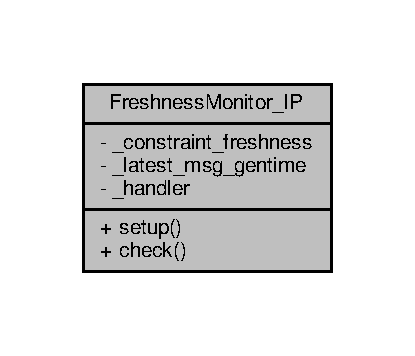
\includegraphics[width=199pt]{classFreshnessMonitor__IP__coll__graph}
\end{center}
\end{figure}
\subsection*{Public 멤버 함수}
\begin{DoxyCompactItemize}
\item 
void \hyperlink{classFreshnessMonitor__IP_a5270577609116294857dbd2192fade7d}{setup} (int64\+\_\+t freshness, void($\ast$\hyperlink{sample__main_8cpp_ae2b580f894f38496da91bce6c31e186f}{freshness\+\_\+handler})())
\item 
int \hyperlink{classFreshnessMonitor__IP_a0527f0f908800c340be5c987e699d0c2}{check} (int64\+\_\+t msg\+\_\+gentime)
\end{DoxyCompactItemize}
\subsection*{Private 속성}
\begin{DoxyCompactItemize}
\item 
int64\+\_\+t \hyperlink{classFreshnessMonitor__IP_ab8e71388a97033da7a0b883bf8f59d44}{\+\_\+constraint\+\_\+freshness} = -\/1
\item 
int64\+\_\+t \hyperlink{classFreshnessMonitor__IP_afb42e4e2c6e1ecc9c40095b513f2147a}{\+\_\+latest\+\_\+msg\+\_\+gentime} = -\/1
\item 
void($\ast$ \hyperlink{classFreshnessMonitor__IP_a299e67c2c338b3c576c712d0f10fc2f3}{\+\_\+handler} )()
\end{DoxyCompactItemize}


\subsection{상세한 설명}
Detect freshness constraint violation. 

\begin{DoxyRefDesc}{할일}
\item[\hyperlink{todo__todo000001}{할일}]modify \hyperlink{classFreshnessMonitor__IP_a0527f0f908800c340be5c987e699d0c2}{check()} to correspond with new definition of message timestamp. \end{DoxyRefDesc}
\begin{DoxyAuthor}{작성자}
Beomjoon Yang 
\end{DoxyAuthor}
\begin{DoxyDate}{날짜}
2018-\/10-\/26 
\end{DoxyDate}
\begin{DoxyVersion}{버전}
0.\+0.\+1 
\end{DoxyVersion}


Processing\+\_\+block.\+cpp 파일의 84 번째 라인에서 정의되었습니다.



\subsection{멤버 함수 문서화}
\index{Freshness\+Monitor\+\_\+\+IP@{Freshness\+Monitor\+\_\+\+IP}!check@{check}}
\index{check@{check}!Freshness\+Monitor\+\_\+\+IP@{Freshness\+Monitor\+\_\+\+IP}}
\subsubsection[{\texorpdfstring{check(int64\+\_\+t msg\+\_\+gentime)}{check(int64_t msg_gentime)}}]{\setlength{\rightskip}{0pt plus 5cm}int Freshness\+Monitor\+\_\+\+I\+P\+::check (
\begin{DoxyParamCaption}
\item[{int64\+\_\+t}]{msg\+\_\+gentime}
\end{DoxyParamCaption}
)}\hypertarget{classFreshnessMonitor__IP_a0527f0f908800c340be5c987e699d0c2}{}\label{classFreshnessMonitor__IP_a0527f0f908800c340be5c987e699d0c2}


Processing\+\_\+block.\+cpp 파일의 101 번째 라인에서 정의되었습니다.



다음을 참조함 \+:  System\+Clock\+::get\+Current\+Time().



다음에 의해서 참조됨 \+:  Input\+Data\+Port\+\_\+\+Fac$<$ Data\+\_\+0, Data\+\_\+1, Data\+\_\+2, Data\+\_\+3, Data\+\_\+4, Data\+\_\+5, Data\+\_\+6, Data\+\_\+7, Data\+\_\+8, Data\+\_\+9 $>$\+::check\+Freshness(), Input\+Data\+Port\+\_\+\+P\+B$<$ Data\+\_\+0, Data\+\_\+1, Data\+\_\+2, Data\+\_\+3, Data\+\_\+4, Data\+\_\+5, Data\+\_\+6, Data\+\_\+7, Data\+\_\+8, Data\+\_\+9 $>$\+::check\+Freshness().



이 함수 내부에서 호출하는 함수들에 대한 그래프입니다.\+:\nopagebreak
\begin{figure}[H]
\begin{center}
\leavevmode
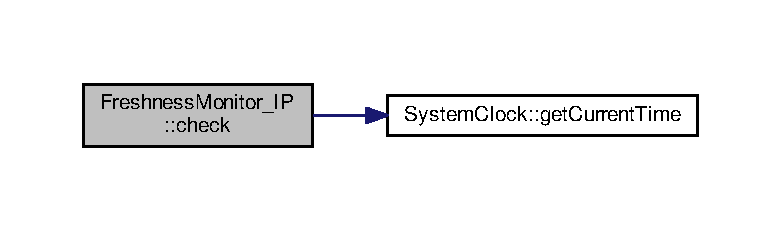
\includegraphics[width=350pt]{classFreshnessMonitor__IP_a0527f0f908800c340be5c987e699d0c2_cgraph}
\end{center}
\end{figure}




이 함수를 호출하는 함수들에 대한 그래프입니다.\+:\nopagebreak
\begin{figure}[H]
\begin{center}
\leavevmode
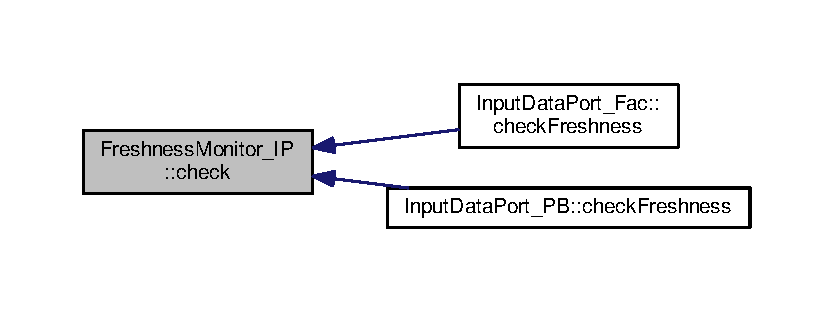
\includegraphics[width=350pt]{classFreshnessMonitor__IP_a0527f0f908800c340be5c987e699d0c2_icgraph}
\end{center}
\end{figure}


\index{Freshness\+Monitor\+\_\+\+IP@{Freshness\+Monitor\+\_\+\+IP}!setup@{setup}}
\index{setup@{setup}!Freshness\+Monitor\+\_\+\+IP@{Freshness\+Monitor\+\_\+\+IP}}
\subsubsection[{\texorpdfstring{setup(int64\+\_\+t freshness, void($\ast$freshness\+\_\+handler)())}{setup(int64_t freshness, void(*freshness_handler)())}}]{\setlength{\rightskip}{0pt plus 5cm}void Freshness\+Monitor\+\_\+\+I\+P\+::setup (
\begin{DoxyParamCaption}
\item[{int64\+\_\+t}]{freshness, }
\item[{void($\ast$)()}]{freshness\+\_\+handler}
\end{DoxyParamCaption}
)}\hypertarget{classFreshnessMonitor__IP_a5270577609116294857dbd2192fade7d}{}\label{classFreshnessMonitor__IP_a5270577609116294857dbd2192fade7d}


Processing\+\_\+block.\+cpp 파일의 95 번째 라인에서 정의되었습니다.



다음을 참조함 \+:  freshness\+\_\+handler().



다음에 의해서 참조됨 \+:  Input\+Data\+Port\+\_\+\+Fac$<$ Data\+\_\+0, Data\+\_\+1, Data\+\_\+2, Data\+\_\+3, Data\+\_\+4, Data\+\_\+5, Data\+\_\+6, Data\+\_\+7, Data\+\_\+8, Data\+\_\+9 $>$\+::set\+Freshness(), Input\+Data\+Port\+\_\+\+P\+B$<$ Data\+\_\+0, Data\+\_\+1, Data\+\_\+2, Data\+\_\+3, Data\+\_\+4, Data\+\_\+5, Data\+\_\+6, Data\+\_\+7, Data\+\_\+8, Data\+\_\+9 $>$\+::set\+Freshness().



이 함수 내부에서 호출하는 함수들에 대한 그래프입니다.\+:\nopagebreak
\begin{figure}[H]
\begin{center}
\leavevmode
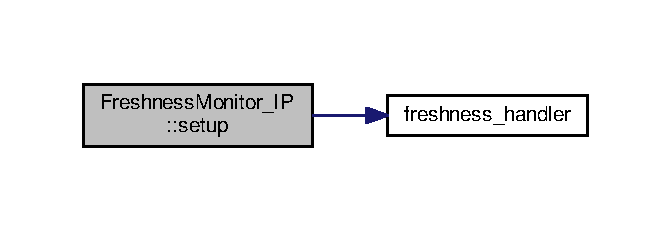
\includegraphics[width=322pt]{classFreshnessMonitor__IP_a5270577609116294857dbd2192fade7d_cgraph}
\end{center}
\end{figure}




이 함수를 호출하는 함수들에 대한 그래프입니다.\+:\nopagebreak
\begin{figure}[H]
\begin{center}
\leavevmode
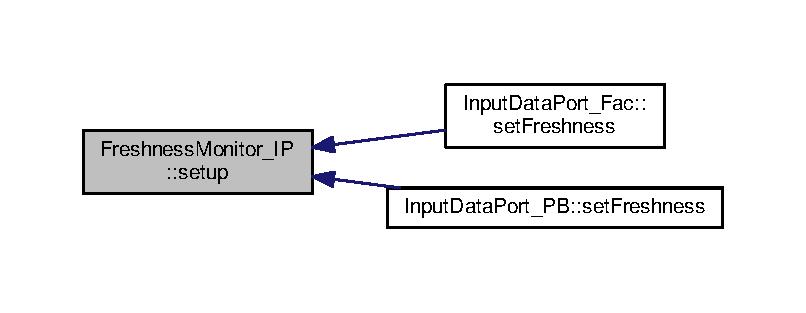
\includegraphics[width=350pt]{classFreshnessMonitor__IP_a5270577609116294857dbd2192fade7d_icgraph}
\end{center}
\end{figure}




\subsection{멤버 데이타 문서화}
\index{Freshness\+Monitor\+\_\+\+IP@{Freshness\+Monitor\+\_\+\+IP}!\+\_\+constraint\+\_\+freshness@{\+\_\+constraint\+\_\+freshness}}
\index{\+\_\+constraint\+\_\+freshness@{\+\_\+constraint\+\_\+freshness}!Freshness\+Monitor\+\_\+\+IP@{Freshness\+Monitor\+\_\+\+IP}}
\subsubsection[{\texorpdfstring{\+\_\+constraint\+\_\+freshness}{_constraint_freshness}}]{\setlength{\rightskip}{0pt plus 5cm}int64\+\_\+t Freshness\+Monitor\+\_\+\+I\+P\+::\+\_\+constraint\+\_\+freshness = -\/1\hspace{0.3cm}{\ttfamily [private]}}\hypertarget{classFreshnessMonitor__IP_ab8e71388a97033da7a0b883bf8f59d44}{}\label{classFreshnessMonitor__IP_ab8e71388a97033da7a0b883bf8f59d44}


Processing\+\_\+block.\+cpp 파일의 90 번째 라인에서 정의되었습니다.

\index{Freshness\+Monitor\+\_\+\+IP@{Freshness\+Monitor\+\_\+\+IP}!\+\_\+handler@{\+\_\+handler}}
\index{\+\_\+handler@{\+\_\+handler}!Freshness\+Monitor\+\_\+\+IP@{Freshness\+Monitor\+\_\+\+IP}}
\subsubsection[{\texorpdfstring{\+\_\+handler}{_handler}}]{\setlength{\rightskip}{0pt plus 5cm}void($\ast$ Freshness\+Monitor\+\_\+\+I\+P\+::\+\_\+handler) ()\hspace{0.3cm}{\ttfamily [private]}}\hypertarget{classFreshnessMonitor__IP_a299e67c2c338b3c576c712d0f10fc2f3}{}\label{classFreshnessMonitor__IP_a299e67c2c338b3c576c712d0f10fc2f3}


Processing\+\_\+block.\+cpp 파일의 92 번째 라인에서 정의되었습니다.

\index{Freshness\+Monitor\+\_\+\+IP@{Freshness\+Monitor\+\_\+\+IP}!\+\_\+latest\+\_\+msg\+\_\+gentime@{\+\_\+latest\+\_\+msg\+\_\+gentime}}
\index{\+\_\+latest\+\_\+msg\+\_\+gentime@{\+\_\+latest\+\_\+msg\+\_\+gentime}!Freshness\+Monitor\+\_\+\+IP@{Freshness\+Monitor\+\_\+\+IP}}
\subsubsection[{\texorpdfstring{\+\_\+latest\+\_\+msg\+\_\+gentime}{_latest_msg_gentime}}]{\setlength{\rightskip}{0pt plus 5cm}int64\+\_\+t Freshness\+Monitor\+\_\+\+I\+P\+::\+\_\+latest\+\_\+msg\+\_\+gentime = -\/1\hspace{0.3cm}{\ttfamily [private]}}\hypertarget{classFreshnessMonitor__IP_afb42e4e2c6e1ecc9c40095b513f2147a}{}\label{classFreshnessMonitor__IP_afb42e4e2c6e1ecc9c40095b513f2147a}


Processing\+\_\+block.\+cpp 파일의 91 번째 라인에서 정의되었습니다.



이 클래스에 대한 문서화 페이지는 다음의 파일로부터 생성되었습니다.\+:\begin{DoxyCompactItemize}
\item 
src/\hyperlink{Processing__block_8cpp}{Processing\+\_\+block.\+cpp}\end{DoxyCompactItemize}

\hypertarget{classFusion__operator}{}\section{Fusion\+\_\+operator$<$ Data\+\_\+0, Data\+\_\+1, Data\+\_\+2, Data\+\_\+3, Data\+\_\+4, Data\+\_\+5, Data\+\_\+6, Data\+\_\+7, Data\+\_\+8, Data\+\_\+9 $>$}
\label{classFusion__operator}\index{Fusion\+\_\+operator$<$ Data\+\_\+0, Data\+\_\+1, Data\+\_\+2, Data\+\_\+3, Data\+\_\+4, Data\+\_\+5, Data\+\_\+6, Data\+\_\+7, Data\+\_\+8, Data\+\_\+9 $>$@{Fusion\+\_\+operator$<$ Data\+\_\+0, Data\+\_\+1, Data\+\_\+2, Data\+\_\+3, Data\+\_\+4, Data\+\_\+5, Data\+\_\+6, Data\+\_\+7, Data\+\_\+8, Data\+\_\+9 $>$}}


Fusion\+\_\+operator$<$ Data\+\_\+0, Data\+\_\+1, Data\+\_\+2, Data\+\_\+3, Data\+\_\+4, Data\+\_\+5, Data\+\_\+6, Data\+\_\+7, Data\+\_\+8, Data\+\_\+9 $>$에 대한 협력 다이어그램\+:\nopagebreak
\begin{figure}[H]
\begin{center}
\leavevmode
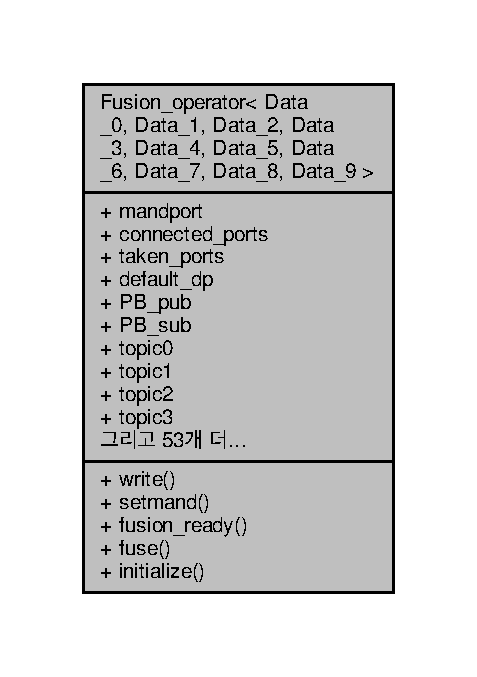
\includegraphics[width=229pt]{classFusion__operator__coll__graph}
\end{center}
\end{figure}
\subsection*{Public 멤버 함수}
\begin{DoxyCompactItemize}
\item 
int \hyperlink{classFusion__operator_a9336f2c0bf50620148cdd404cc139843}{write} (Data\+\_\+9)
\item 
int \hyperlink{classFusion__operator_a132cd952907c90ae57ede626900d42c1}{setmand} (std\+::bitset$<$ 9 $>$ $\ast$)
\item 
void \hyperlink{classFusion__operator_adc41869c62a2702bcdf55c124cbf279c}{fusion\+\_\+ready} ()
\item 
void \hyperlink{classFusion__operator_a3f543c87eea905946c33e1a00bcc4e0b}{fuse} ()
\item 
void \hyperlink{classFusion__operator_a6e5a527e137d815675137e195a81bc8c}{initialize} (std\+::string name, double correlation, int opt\+\_\+count, int core\+\_\+id)
\end{DoxyCompactItemize}
\subsection*{Public 속성}
\begin{DoxyCompactItemize}
\item 
std\+::bitset$<$ 9 $>$ \hyperlink{classFusion__operator_a1b0feb66d902358293e42a9cea02b5f7}{mandport}
\item 
std\+::bitset$<$ 10 $>$ \hyperlink{classFusion__operator_a5d5904ab66f3b43ed107a5b3ef9d205b}{connected\+\_\+ports}
\item 
std\+::bitset$<$ 9 $>$ \hyperlink{classFusion__operator_a29bdb5e13d8f8adf00ffcfcbca60fcf4}{taken\+\_\+ports}
\item 
dds\+::domain\+::\+Domain\+Participant \hyperlink{classFusion__operator_ad3b3aafd9ed9aa55eb097656a97551bd}{default\+\_\+dp} \{org\+::opensplice\+::domain\+::default\+\_\+id()\}
\item 
dds\+::pub\+::\+Publisher \hyperlink{classFusion__operator_a121024c841142a5b50be10b19e94653e}{P\+B\+\_\+pub} \{\hyperlink{classFusion__operator_ad3b3aafd9ed9aa55eb097656a97551bd}{default\+\_\+dp}, default\+\_\+dp.\+default\+\_\+publisher\+\_\+qos()\}
\item 
dds\+::sub\+::\+Subscriber \hyperlink{classFusion__operator_aa22d9bbeb385dc5b1e31d85d65d63f28}{P\+B\+\_\+sub} \{\hyperlink{classFusion__operator_ad3b3aafd9ed9aa55eb097656a97551bd}{default\+\_\+dp}, default\+\_\+dp.\+default\+\_\+subscriber\+\_\+qos()\}
\item 
dds\+::topic\+::\+Topic$<$ Data\+\_\+0 $>$ $\ast$ \hyperlink{classFusion__operator_a378e811778586da6619a1d6c2d1c5f37}{topic0}
\item 
dds\+::topic\+::\+Topic$<$ Data\+\_\+1 $>$ $\ast$ \hyperlink{classFusion__operator_a79543a848dd9ac2cb01f9e38acf2b988}{topic1}
\item 
dds\+::topic\+::\+Topic$<$ Data\+\_\+2 $>$ $\ast$ \hyperlink{classFusion__operator_a156ba17873325c431689c47f2f2d6296}{topic2}
\item 
dds\+::topic\+::\+Topic$<$ Data\+\_\+3 $>$ $\ast$ \hyperlink{classFusion__operator_af90486f24e7f5e82364b20ad9d448595}{topic3}
\item 
dds\+::topic\+::\+Topic$<$ Data\+\_\+4 $>$ $\ast$ \hyperlink{classFusion__operator_a2436ee57380c11e74b971df67d23c06a}{topic4}
\item 
dds\+::topic\+::\+Topic$<$ Data\+\_\+5 $>$ $\ast$ \hyperlink{classFusion__operator_a610b159b6f22ca65f11d2db2c1b2124b}{topic5}
\item 
dds\+::topic\+::\+Topic$<$ Data\+\_\+6 $>$ $\ast$ \hyperlink{classFusion__operator_a747b20c14e1a835bb763694a1368d857}{topic6}
\item 
dds\+::topic\+::\+Topic$<$ Data\+\_\+7 $>$ $\ast$ \hyperlink{classFusion__operator_abeb8122aebb4d834cb3433aaa99365dd}{topic7}
\item 
dds\+::topic\+::\+Topic$<$ Data\+\_\+8 $>$ $\ast$ \hyperlink{classFusion__operator_ab050a3199eb223c53a60087961d0e0cc}{topic8}
\item 
dds\+::topic\+::\+Topic$<$ Data\+\_\+9 $>$ $\ast$ \hyperlink{classFusion__operator_afb0a94863c813bbc7fc2a52838301937}{topic9}
\item 
dds\+::topic\+::\+Topic$<$ int $>$ $\ast$ \hyperlink{classFusion__operator_ab2ba1dc33bae5f39ecabd4018bedf47f}{topic\+\_\+event}
\item 
dds\+::core\+::cond\+::\+Wait\+Set \hyperlink{classFusion__operator_a15a7b6ccddbe0b8ad3bd8932a38c6db2}{ws\+\_\+0}
\item 
dds\+::core\+::cond\+::\+Wait\+Set \hyperlink{classFusion__operator_a6ca4a3185f87b382542eaf241eab3e52}{ws\+\_\+1}
\item 
dds\+::core\+::cond\+::\+Wait\+Set \hyperlink{classFusion__operator_af231872d2c22b353710ee90b6a2be4bf}{ws\+\_\+2}
\item 
dds\+::core\+::cond\+::\+Wait\+Set \hyperlink{classFusion__operator_a31133e7918c57cbca7cc42f141ff672d}{ws\+\_\+3}
\item 
dds\+::core\+::cond\+::\+Wait\+Set \hyperlink{classFusion__operator_a5dea84d5320494140d650bc0823d56f2}{ws\+\_\+4}
\item 
dds\+::core\+::cond\+::\+Wait\+Set \hyperlink{classFusion__operator_ac2bc73cfd2d097373d0716e61c843a33}{ws\+\_\+5}
\item 
dds\+::core\+::cond\+::\+Wait\+Set \hyperlink{classFusion__operator_a32e2694d512a9ba74b13a0b07f8f4649}{ws\+\_\+6}
\item 
dds\+::core\+::cond\+::\+Wait\+Set \hyperlink{classFusion__operator_a0c468d5a6c0fb3b6adf93372ca678c65}{ws\+\_\+7}
\item 
dds\+::core\+::cond\+::\+Wait\+Set \hyperlink{classFusion__operator_a07930a190539ebefac664cc34d81dbe8}{ws\+\_\+8}
\item 
\hyperlink{classInputDataPort__F}{Input\+Data\+Port\+\_\+F}$<$ Data\+\_\+0, Data\+\_\+1, Data\+\_\+2, Data\+\_\+3, Data\+\_\+4, Data\+\_\+5, Data\+\_\+6, Data\+\_\+7, Data\+\_\+8, Data\+\_\+9 $>$ $\ast$ \hyperlink{classFusion__operator_a7bcb3db4950e0de858fcd1e481e987d9}{I\+D\+P0}
\item 
\hyperlink{classInputDataPort__F}{Input\+Data\+Port\+\_\+F}$<$ Data\+\_\+0, Data\+\_\+1, Data\+\_\+2, Data\+\_\+3, Data\+\_\+4, Data\+\_\+5, Data\+\_\+6, Data\+\_\+7, Data\+\_\+8, Data\+\_\+9 $>$ $\ast$ \hyperlink{classFusion__operator_a758f7524bb515cb07df2cbac6b06cef4}{I\+D\+P1}
\item 
\hyperlink{classInputDataPort__F}{Input\+Data\+Port\+\_\+F}$<$ Data\+\_\+0, Data\+\_\+1, Data\+\_\+2, Data\+\_\+3, Data\+\_\+4, Data\+\_\+5, Data\+\_\+6, Data\+\_\+7, Data\+\_\+8, Data\+\_\+9 $>$ $\ast$ \hyperlink{classFusion__operator_a1c237055f4af1bfed7d18f0f1620b5dc}{I\+D\+P2}
\item 
\hyperlink{classInputDataPort__F}{Input\+Data\+Port\+\_\+F}$<$ Data\+\_\+0, Data\+\_\+1, Data\+\_\+2, Data\+\_\+3, Data\+\_\+4, Data\+\_\+5, Data\+\_\+6, Data\+\_\+7, Data\+\_\+8, Data\+\_\+9 $>$ $\ast$ \hyperlink{classFusion__operator_ae053a7964cd7ba4422303dddda22bb8c}{I\+D\+P3}
\item 
\hyperlink{classInputDataPort__F}{Input\+Data\+Port\+\_\+F}$<$ Data\+\_\+0, Data\+\_\+1, Data\+\_\+2, Data\+\_\+3, Data\+\_\+4, Data\+\_\+5, Data\+\_\+6, Data\+\_\+7, Data\+\_\+8, Data\+\_\+9 $>$ $\ast$ \hyperlink{classFusion__operator_a087dec92bca6e8c5c9f3a8c033db66c2}{I\+D\+P4}
\item 
\hyperlink{classInputDataPort__F}{Input\+Data\+Port\+\_\+F}$<$ Data\+\_\+0, Data\+\_\+1, Data\+\_\+2, Data\+\_\+3, Data\+\_\+4, Data\+\_\+5, Data\+\_\+6, Data\+\_\+7, Data\+\_\+8, Data\+\_\+9 $>$ $\ast$ \hyperlink{classFusion__operator_ae1ea70ef80557cc22efefb7cb5bae955}{I\+D\+P5}
\item 
\hyperlink{classInputDataPort__F}{Input\+Data\+Port\+\_\+F}$<$ Data\+\_\+0, Data\+\_\+1, Data\+\_\+2, Data\+\_\+3, Data\+\_\+4, Data\+\_\+5, Data\+\_\+6, Data\+\_\+7, Data\+\_\+8, Data\+\_\+9 $>$ $\ast$ \hyperlink{classFusion__operator_a380165fcccb240f43de928c329b93ddf}{I\+D\+P6}
\item 
\hyperlink{classInputDataPort__F}{Input\+Data\+Port\+\_\+F}$<$ Data\+\_\+0, Data\+\_\+1, Data\+\_\+2, Data\+\_\+3, Data\+\_\+4, Data\+\_\+5, Data\+\_\+6, Data\+\_\+7, Data\+\_\+8, Data\+\_\+9 $>$ $\ast$ \hyperlink{classFusion__operator_a03fa8722d419112cc6f9d21354453985}{I\+D\+P7}
\item 
\hyperlink{classInputDataPort__F}{Input\+Data\+Port\+\_\+F}$<$ Data\+\_\+0, Data\+\_\+1, Data\+\_\+2, Data\+\_\+3, Data\+\_\+4, Data\+\_\+5, Data\+\_\+6, Data\+\_\+7, Data\+\_\+8, Data\+\_\+9 $>$ $\ast$ \hyperlink{classFusion__operator_afdf3f278a54f1dfeb655889ab7ec9ce7}{I\+D\+P8}
\item 
\hyperlink{classOutputDataPort__F}{Output\+Data\+Port\+\_\+F}$<$ Data\+\_\+0, Data\+\_\+1, Data\+\_\+2, Data\+\_\+3, Data\+\_\+4, Data\+\_\+5, Data\+\_\+6, Data\+\_\+7, Data\+\_\+8, Data\+\_\+9 $>$ $\ast$ \hyperlink{classFusion__operator_a3afeb436d521b3c232ac41e26193ef3b}{O\+DP}
\item 
dds\+::sub\+::\+Sample$<$ Data\+\_\+0 $>$ \hyperlink{classFusion__operator_accd0def1ab312df9918676814257da82}{fusion\+\_\+data1}
\item 
dds\+::sub\+::\+Sample$<$ Data\+\_\+1 $>$ \hyperlink{classFusion__operator_a8c545bb751bfdda39be20b56b4aa7cbc}{fusion\+\_\+data2}
\item 
dds\+::sub\+::\+Sample$<$ Data\+\_\+2 $>$ \hyperlink{classFusion__operator_a983008a895d0902a9aafc471af7681a5}{fusion\+\_\+data3}
\item 
dds\+::sub\+::\+Sample$<$ Data\+\_\+3 $>$ \hyperlink{classFusion__operator_a40f85d88738eca58c412f0b70792678f}{fusion\+\_\+data4}
\item 
dds\+::sub\+::\+Sample$<$ Data\+\_\+4 $>$ \hyperlink{classFusion__operator_a770f79170f64f611facd933ebb1c9b58}{fusion\+\_\+data5}
\item 
dds\+::sub\+::\+Sample$<$ Data\+\_\+5 $>$ \hyperlink{classFusion__operator_ab60db5c3be3d0512a35c4231616383c4}{fusion\+\_\+data6}
\item 
dds\+::sub\+::\+Sample$<$ Data\+\_\+6 $>$ \hyperlink{classFusion__operator_a12845b96c8a2a00cbf7290462e2fa215}{fusion\+\_\+data7}
\item 
dds\+::sub\+::\+Sample$<$ Data\+\_\+7 $>$ \hyperlink{classFusion__operator_ac3ddeea7acd61121e02501cbffc2b7be}{fusion\+\_\+data8}
\item 
dds\+::sub\+::\+Sample$<$ Data\+\_\+8 $>$ \hyperlink{classFusion__operator_af352606f5dcf540b5e9beb72870c9fa6}{fusion\+\_\+data9}
\item 
std\+::vector$<$ dds\+::sub\+::\+Sample$<$ Data\+\_\+0 $>$ $>$ \hyperlink{classFusion__operator_ab24eda6a56115e1eb0ab2c89a2632436}{sample\+\_\+0} \{1\}
\item 
std\+::vector$<$ dds\+::sub\+::\+Sample$<$ Data\+\_\+0 $>$ $>$\+::iterator \hyperlink{classFusion__operator_ab0adcc22beac8918ea3e22b04f1d31d3}{iter\+\_\+0}
\item 
std\+::vector$<$ dds\+::sub\+::\+Sample$<$ Data\+\_\+1 $>$ $>$ \hyperlink{classFusion__operator_afe367eeae918067d7d26c90bc0be202d}{sample\+\_\+1} \{1\}
\item 
std\+::vector$<$ dds\+::sub\+::\+Sample$<$ Data\+\_\+1 $>$ $>$\+::iterator \hyperlink{classFusion__operator_a4d552a9a1ab0911598232059cb0937bc}{iter\+\_\+1}
\item 
std\+::vector$<$ dds\+::sub\+::\+Sample$<$ Data\+\_\+2 $>$ $>$ \hyperlink{classFusion__operator_a1a65f84d529180cd77defee525bc7bd6}{sample\+\_\+2} \{1\}
\item 
std\+::vector$<$ dds\+::sub\+::\+Sample$<$ Data\+\_\+2 $>$ $>$\+::iterator \hyperlink{classFusion__operator_a4fd31cb3bea3e7362643729b4bdcb3f1}{iter\+\_\+2}
\item 
std\+::vector$<$ dds\+::sub\+::\+Sample$<$ Data\+\_\+3 $>$ $>$ \hyperlink{classFusion__operator_a1954d8d67f9a34d47e5b59cc65d09252}{sample\+\_\+3} \{1\}
\item 
std\+::vector$<$ dds\+::sub\+::\+Sample$<$ Data\+\_\+3 $>$ $>$\+::iterator \hyperlink{classFusion__operator_a15048a8432350604c31fbbd6945d4692}{iter\+\_\+3}
\item 
std\+::vector$<$ dds\+::sub\+::\+Sample$<$ Data\+\_\+4 $>$ $>$ \hyperlink{classFusion__operator_a56bb3464ca6d140acdf3560bb94a401b}{sample\+\_\+4} \{1\}
\item 
std\+::vector$<$ dds\+::sub\+::\+Sample$<$ Data\+\_\+4 $>$ $>$\+::iterator \hyperlink{classFusion__operator_a98de1068d698554103ec8b77a012df5b}{iter\+\_\+4}
\item 
std\+::vector$<$ dds\+::sub\+::\+Sample$<$ Data\+\_\+5 $>$ $>$ \hyperlink{classFusion__operator_a5623c0acc7a90d21a50ac010a5f1daf5}{sample\+\_\+5} \{1\}
\item 
std\+::vector$<$ dds\+::sub\+::\+Sample$<$ Data\+\_\+5 $>$ $>$\+::iterator \hyperlink{classFusion__operator_a323bf6a71abd728d9ef6daa5ed1b1ab2}{iter\+\_\+5}
\item 
std\+::vector$<$ dds\+::sub\+::\+Sample$<$ Data\+\_\+6 $>$ $>$ \hyperlink{classFusion__operator_a0051d8d0ba3e16b797e38412e44f46ef}{sample\+\_\+6} \{1\}
\item 
std\+::vector$<$ dds\+::sub\+::\+Sample$<$ Data\+\_\+6 $>$ $>$\+::iterator \hyperlink{classFusion__operator_a38913c414f92a70db936c629ddfb4fb0}{iter\+\_\+6}
\item 
std\+::vector$<$ dds\+::sub\+::\+Sample$<$ Data\+\_\+7 $>$ $>$ \hyperlink{classFusion__operator_ac206ae8fc1c89e2ca114bb80a5899bcd}{sample\+\_\+7} \{1\}
\item 
std\+::vector$<$ dds\+::sub\+::\+Sample$<$ Data\+\_\+7 $>$ $>$\+::iterator \hyperlink{classFusion__operator_a010f79ae83cd86608e81475c4b021104}{iter\+\_\+7}
\item 
std\+::vector$<$ dds\+::sub\+::\+Sample$<$ Data\+\_\+8 $>$ $>$ \hyperlink{classFusion__operator_ad74fbf7634ca557dc8e590487b21b283}{sample\+\_\+8} \{1\}
\item 
std\+::vector$<$ dds\+::sub\+::\+Sample$<$ Data\+\_\+8 $>$ $>$\+::iterator \hyperlink{classFusion__operator_a472aa52f1d6fb1646283d5d955a13ae1}{iter\+\_\+8}
\end{DoxyCompactItemize}


\subsection{상세한 설명}
\subsubsection*{template$<$typename Data\+\_\+0, typename Data\+\_\+1, typename Data\+\_\+2, typename Data\+\_\+3, typename Data\+\_\+4, typename Data\+\_\+5, typename Data\+\_\+6, typename Data\+\_\+7, typename Data\+\_\+8, typename Data\+\_\+9$>$\\*
class Fusion\+\_\+operator$<$ Data\+\_\+0, Data\+\_\+1, Data\+\_\+2, Data\+\_\+3, Data\+\_\+4, Data\+\_\+5, Data\+\_\+6, Data\+\_\+7, Data\+\_\+8, Data\+\_\+9 $>$}



Fusion\+\_\+operator.\+cpp 파일의 49 번째 라인에서 정의되었습니다.



\subsection{멤버 함수 문서화}
\index{Fusion\+\_\+operator@{Fusion\+\_\+operator}!fuse@{fuse}}
\index{fuse@{fuse}!Fusion\+\_\+operator@{Fusion\+\_\+operator}}
\subsubsection[{\texorpdfstring{fuse()}{fuse()}}]{\setlength{\rightskip}{0pt plus 5cm}template$<$typename Data\+\_\+0 , typename Data\+\_\+1 , typename Data\+\_\+2 , typename Data\+\_\+3 , typename Data\+\_\+4 , typename Data\+\_\+5 , typename Data\+\_\+6 , typename Data\+\_\+7 , typename Data\+\_\+8 , typename Data\+\_\+9 $>$ void {\bf Fusion\+\_\+operator}$<$ Data\+\_\+0, Data\+\_\+1, Data\+\_\+2, Data\+\_\+3, Data\+\_\+4, Data\+\_\+5, Data\+\_\+6, Data\+\_\+7, Data\+\_\+8, Data\+\_\+9 $>$\+::fuse (
\begin{DoxyParamCaption}
{}
\end{DoxyParamCaption}
)}\hypertarget{classFusion__operator_a3f543c87eea905946c33e1a00bcc4e0b}{}\label{classFusion__operator_a3f543c87eea905946c33e1a00bcc4e0b}


sample\+\_\+main\+\_\+2.\+cpp 파일의 36 번째 라인에서 정의되었습니다.

\index{Fusion\+\_\+operator@{Fusion\+\_\+operator}!fusion\+\_\+ready@{fusion\+\_\+ready}}
\index{fusion\+\_\+ready@{fusion\+\_\+ready}!Fusion\+\_\+operator@{Fusion\+\_\+operator}}
\subsubsection[{\texorpdfstring{fusion\+\_\+ready()}{fusion_ready()}}]{\setlength{\rightskip}{0pt plus 5cm}template$<$typename Data\+\_\+0 , typename Data\+\_\+1 , typename Data\+\_\+2 , typename Data\+\_\+3 , typename Data\+\_\+4 , typename Data\+\_\+5 , typename Data\+\_\+6 , typename Data\+\_\+7 , typename Data\+\_\+8 , typename Data\+\_\+9 $>$ void {\bf Fusion\+\_\+operator}$<$ Data\+\_\+0, Data\+\_\+1, Data\+\_\+2, Data\+\_\+3, Data\+\_\+4, Data\+\_\+5, Data\+\_\+6, Data\+\_\+7, Data\+\_\+8, Data\+\_\+9 $>$\+::fusion\+\_\+ready (
\begin{DoxyParamCaption}
{}
\end{DoxyParamCaption}
)}\hypertarget{classFusion__operator_adc41869c62a2702bcdf55c124cbf279c}{}\label{classFusion__operator_adc41869c62a2702bcdf55c124cbf279c}


Fusion\+\_\+operator.\+cpp 파일의 551 번째 라인에서 정의되었습니다.

\index{Fusion\+\_\+operator@{Fusion\+\_\+operator}!initialize@{initialize}}
\index{initialize@{initialize}!Fusion\+\_\+operator@{Fusion\+\_\+operator}}
\subsubsection[{\texorpdfstring{initialize(std\+::string name, double correlation, int opt\+\_\+count, int core\+\_\+id)}{initialize(std::string name, double correlation, int opt_count, int core_id)}}]{\setlength{\rightskip}{0pt plus 5cm}template$<$typename Data\+\_\+0 , typename Data\+\_\+1 , typename Data\+\_\+2 , typename Data\+\_\+3 , typename Data\+\_\+4 , typename Data\+\_\+5 , typename Data\+\_\+6 , typename Data\+\_\+7 , typename Data\+\_\+8 , typename Data\+\_\+9 $>$ void {\bf Fusion\+\_\+operator}$<$ Data\+\_\+0, Data\+\_\+1, Data\+\_\+2, Data\+\_\+3, Data\+\_\+4, Data\+\_\+5, Data\+\_\+6, Data\+\_\+7, Data\+\_\+8, Data\+\_\+9 $>$\+::initialize (
\begin{DoxyParamCaption}
\item[{std\+::string}]{name, }
\item[{double}]{correlation, }
\item[{int}]{opt\+\_\+count, }
\item[{int}]{core\+\_\+id}
\end{DoxyParamCaption}
)}\hypertarget{classFusion__operator_a6e5a527e137d815675137e195a81bc8c}{}\label{classFusion__operator_a6e5a527e137d815675137e195a81bc8c}


Fusion\+\_\+operator.\+cpp 파일의 743 번째 라인에서 정의되었습니다.

\index{Fusion\+\_\+operator@{Fusion\+\_\+operator}!setmand@{setmand}}
\index{setmand@{setmand}!Fusion\+\_\+operator@{Fusion\+\_\+operator}}
\subsubsection[{\texorpdfstring{setmand(std\+::bitset$<$ 9 $>$ $\ast$)}{setmand(std::bitset< 9 > *)}}]{\setlength{\rightskip}{0pt plus 5cm}template$<$typename Data\+\_\+0, typename Data\+\_\+1, typename Data\+\_\+2, typename Data\+\_\+3, typename Data\+\_\+4, typename Data\+\_\+5, typename Data\+\_\+6, typename Data\+\_\+7, typename Data\+\_\+8, typename Data\+\_\+9$>$ int {\bf Fusion\+\_\+operator}$<$ Data\+\_\+0, Data\+\_\+1, Data\+\_\+2, Data\+\_\+3, Data\+\_\+4, Data\+\_\+5, Data\+\_\+6, Data\+\_\+7, Data\+\_\+8, Data\+\_\+9 $>$\+::setmand (
\begin{DoxyParamCaption}
\item[{std\+::bitset$<$ 9 $>$ $\ast$}]{}
\end{DoxyParamCaption}
)}\hypertarget{classFusion__operator_a132cd952907c90ae57ede626900d42c1}{}\label{classFusion__operator_a132cd952907c90ae57ede626900d42c1}
\index{Fusion\+\_\+operator@{Fusion\+\_\+operator}!write@{write}}
\index{write@{write}!Fusion\+\_\+operator@{Fusion\+\_\+operator}}
\subsubsection[{\texorpdfstring{write(\+Data\+\_\+9)}{write(Data_9)}}]{\setlength{\rightskip}{0pt plus 5cm}template$<$typename Data\+\_\+0 , typename Data\+\_\+1 , typename Data\+\_\+2 , typename Data\+\_\+3 , typename Data\+\_\+4 , typename Data\+\_\+5 , typename Data\+\_\+6 , typename Data\+\_\+7 , typename Data\+\_\+8 , typename Data\+\_\+9 $>$ int {\bf Fusion\+\_\+operator}$<$ Data\+\_\+0, Data\+\_\+1, Data\+\_\+2, Data\+\_\+3, Data\+\_\+4, Data\+\_\+5, Data\+\_\+6, Data\+\_\+7, Data\+\_\+8, Data\+\_\+9 $>$\+::write (
\begin{DoxyParamCaption}
\item[{Data\+\_\+9}]{Data}
\end{DoxyParamCaption}
)}\hypertarget{classFusion__operator_a9336f2c0bf50620148cdd404cc139843}{}\label{classFusion__operator_a9336f2c0bf50620148cdd404cc139843}


Fusion\+\_\+operator.\+cpp 파일의 539 번째 라인에서 정의되었습니다.



\subsection{멤버 데이타 문서화}
\index{Fusion\+\_\+operator@{Fusion\+\_\+operator}!connected\+\_\+ports@{connected\+\_\+ports}}
\index{connected\+\_\+ports@{connected\+\_\+ports}!Fusion\+\_\+operator@{Fusion\+\_\+operator}}
\subsubsection[{\texorpdfstring{connected\+\_\+ports}{connected_ports}}]{\setlength{\rightskip}{0pt plus 5cm}template$<$typename Data\+\_\+0, typename Data\+\_\+1, typename Data\+\_\+2, typename Data\+\_\+3, typename Data\+\_\+4, typename Data\+\_\+5, typename Data\+\_\+6, typename Data\+\_\+7, typename Data\+\_\+8, typename Data\+\_\+9$>$ std\+::bitset$<$10$>$ {\bf Fusion\+\_\+operator}$<$ Data\+\_\+0, Data\+\_\+1, Data\+\_\+2, Data\+\_\+3, Data\+\_\+4, Data\+\_\+5, Data\+\_\+6, Data\+\_\+7, Data\+\_\+8, Data\+\_\+9 $>$\+::connected\+\_\+ports}\hypertarget{classFusion__operator_a5d5904ab66f3b43ed107a5b3ef9d205b}{}\label{classFusion__operator_a5d5904ab66f3b43ed107a5b3ef9d205b}


Fusion\+\_\+operator.\+cpp 파일의 55 번째 라인에서 정의되었습니다.



다음에 의해서 참조됨 \+:  Input\+Data\+Port\+\_\+\+F$<$ Data\+\_\+0, Data\+\_\+1, Data\+\_\+2, Data\+\_\+3, Data\+\_\+4, Data\+\_\+5, Data\+\_\+6, Data\+\_\+7, Data\+\_\+8, Data\+\_\+9 $>$\+::attach(), Output\+Data\+Port\+\_\+\+F$<$ Data\+\_\+0, Data\+\_\+1, Data\+\_\+2, Data\+\_\+3, Data\+\_\+4, Data\+\_\+5, Data\+\_\+6, Data\+\_\+7, Data\+\_\+8, Data\+\_\+9 $>$\+::attach().

\index{Fusion\+\_\+operator@{Fusion\+\_\+operator}!default\+\_\+dp@{default\+\_\+dp}}
\index{default\+\_\+dp@{default\+\_\+dp}!Fusion\+\_\+operator@{Fusion\+\_\+operator}}
\subsubsection[{\texorpdfstring{default\+\_\+dp}{default_dp}}]{\setlength{\rightskip}{0pt plus 5cm}template$<$typename Data\+\_\+0, typename Data\+\_\+1, typename Data\+\_\+2, typename Data\+\_\+3, typename Data\+\_\+4, typename Data\+\_\+5, typename Data\+\_\+6, typename Data\+\_\+7, typename Data\+\_\+8, typename Data\+\_\+9$>$ dds\+::domain\+::\+Domain\+Participant {\bf Fusion\+\_\+operator}$<$ Data\+\_\+0, Data\+\_\+1, Data\+\_\+2, Data\+\_\+3, Data\+\_\+4, Data\+\_\+5, Data\+\_\+6, Data\+\_\+7, Data\+\_\+8, Data\+\_\+9 $>$\+::default\+\_\+dp \{org\+::opensplice\+::domain\+::default\+\_\+id()\}}\hypertarget{classFusion__operator_ad3b3aafd9ed9aa55eb097656a97551bd}{}\label{classFusion__operator_ad3b3aafd9ed9aa55eb097656a97551bd}


Fusion\+\_\+operator.\+cpp 파일의 58 번째 라인에서 정의되었습니다.

\index{Fusion\+\_\+operator@{Fusion\+\_\+operator}!fusion\+\_\+data1@{fusion\+\_\+data1}}
\index{fusion\+\_\+data1@{fusion\+\_\+data1}!Fusion\+\_\+operator@{Fusion\+\_\+operator}}
\subsubsection[{\texorpdfstring{fusion\+\_\+data1}{fusion_data1}}]{\setlength{\rightskip}{0pt plus 5cm}template$<$typename Data\+\_\+0, typename Data\+\_\+1, typename Data\+\_\+2, typename Data\+\_\+3, typename Data\+\_\+4, typename Data\+\_\+5, typename Data\+\_\+6, typename Data\+\_\+7, typename Data\+\_\+8, typename Data\+\_\+9$>$ dds\+::sub\+::\+Sample$<$Data\+\_\+0$>$ {\bf Fusion\+\_\+operator}$<$ Data\+\_\+0, Data\+\_\+1, Data\+\_\+2, Data\+\_\+3, Data\+\_\+4, Data\+\_\+5, Data\+\_\+6, Data\+\_\+7, Data\+\_\+8, Data\+\_\+9 $>$\+::fusion\+\_\+data1}\hypertarget{classFusion__operator_accd0def1ab312df9918676814257da82}{}\label{classFusion__operator_accd0def1ab312df9918676814257da82}


Fusion\+\_\+operator.\+cpp 파일의 148 번째 라인에서 정의되었습니다.

\index{Fusion\+\_\+operator@{Fusion\+\_\+operator}!fusion\+\_\+data2@{fusion\+\_\+data2}}
\index{fusion\+\_\+data2@{fusion\+\_\+data2}!Fusion\+\_\+operator@{Fusion\+\_\+operator}}
\subsubsection[{\texorpdfstring{fusion\+\_\+data2}{fusion_data2}}]{\setlength{\rightskip}{0pt plus 5cm}template$<$typename Data\+\_\+0, typename Data\+\_\+1, typename Data\+\_\+2, typename Data\+\_\+3, typename Data\+\_\+4, typename Data\+\_\+5, typename Data\+\_\+6, typename Data\+\_\+7, typename Data\+\_\+8, typename Data\+\_\+9$>$ dds\+::sub\+::\+Sample$<$Data\+\_\+1$>$ {\bf Fusion\+\_\+operator}$<$ Data\+\_\+0, Data\+\_\+1, Data\+\_\+2, Data\+\_\+3, Data\+\_\+4, Data\+\_\+5, Data\+\_\+6, Data\+\_\+7, Data\+\_\+8, Data\+\_\+9 $>$\+::fusion\+\_\+data2}\hypertarget{classFusion__operator_a8c545bb751bfdda39be20b56b4aa7cbc}{}\label{classFusion__operator_a8c545bb751bfdda39be20b56b4aa7cbc}


Fusion\+\_\+operator.\+cpp 파일의 149 번째 라인에서 정의되었습니다.

\index{Fusion\+\_\+operator@{Fusion\+\_\+operator}!fusion\+\_\+data3@{fusion\+\_\+data3}}
\index{fusion\+\_\+data3@{fusion\+\_\+data3}!Fusion\+\_\+operator@{Fusion\+\_\+operator}}
\subsubsection[{\texorpdfstring{fusion\+\_\+data3}{fusion_data3}}]{\setlength{\rightskip}{0pt plus 5cm}template$<$typename Data\+\_\+0, typename Data\+\_\+1, typename Data\+\_\+2, typename Data\+\_\+3, typename Data\+\_\+4, typename Data\+\_\+5, typename Data\+\_\+6, typename Data\+\_\+7, typename Data\+\_\+8, typename Data\+\_\+9$>$ dds\+::sub\+::\+Sample$<$Data\+\_\+2$>$ {\bf Fusion\+\_\+operator}$<$ Data\+\_\+0, Data\+\_\+1, Data\+\_\+2, Data\+\_\+3, Data\+\_\+4, Data\+\_\+5, Data\+\_\+6, Data\+\_\+7, Data\+\_\+8, Data\+\_\+9 $>$\+::fusion\+\_\+data3}\hypertarget{classFusion__operator_a983008a895d0902a9aafc471af7681a5}{}\label{classFusion__operator_a983008a895d0902a9aafc471af7681a5}


Fusion\+\_\+operator.\+cpp 파일의 150 번째 라인에서 정의되었습니다.

\index{Fusion\+\_\+operator@{Fusion\+\_\+operator}!fusion\+\_\+data4@{fusion\+\_\+data4}}
\index{fusion\+\_\+data4@{fusion\+\_\+data4}!Fusion\+\_\+operator@{Fusion\+\_\+operator}}
\subsubsection[{\texorpdfstring{fusion\+\_\+data4}{fusion_data4}}]{\setlength{\rightskip}{0pt plus 5cm}template$<$typename Data\+\_\+0, typename Data\+\_\+1, typename Data\+\_\+2, typename Data\+\_\+3, typename Data\+\_\+4, typename Data\+\_\+5, typename Data\+\_\+6, typename Data\+\_\+7, typename Data\+\_\+8, typename Data\+\_\+9$>$ dds\+::sub\+::\+Sample$<$Data\+\_\+3$>$ {\bf Fusion\+\_\+operator}$<$ Data\+\_\+0, Data\+\_\+1, Data\+\_\+2, Data\+\_\+3, Data\+\_\+4, Data\+\_\+5, Data\+\_\+6, Data\+\_\+7, Data\+\_\+8, Data\+\_\+9 $>$\+::fusion\+\_\+data4}\hypertarget{classFusion__operator_a40f85d88738eca58c412f0b70792678f}{}\label{classFusion__operator_a40f85d88738eca58c412f0b70792678f}


Fusion\+\_\+operator.\+cpp 파일의 151 번째 라인에서 정의되었습니다.

\index{Fusion\+\_\+operator@{Fusion\+\_\+operator}!fusion\+\_\+data5@{fusion\+\_\+data5}}
\index{fusion\+\_\+data5@{fusion\+\_\+data5}!Fusion\+\_\+operator@{Fusion\+\_\+operator}}
\subsubsection[{\texorpdfstring{fusion\+\_\+data5}{fusion_data5}}]{\setlength{\rightskip}{0pt plus 5cm}template$<$typename Data\+\_\+0, typename Data\+\_\+1, typename Data\+\_\+2, typename Data\+\_\+3, typename Data\+\_\+4, typename Data\+\_\+5, typename Data\+\_\+6, typename Data\+\_\+7, typename Data\+\_\+8, typename Data\+\_\+9$>$ dds\+::sub\+::\+Sample$<$Data\+\_\+4$>$ {\bf Fusion\+\_\+operator}$<$ Data\+\_\+0, Data\+\_\+1, Data\+\_\+2, Data\+\_\+3, Data\+\_\+4, Data\+\_\+5, Data\+\_\+6, Data\+\_\+7, Data\+\_\+8, Data\+\_\+9 $>$\+::fusion\+\_\+data5}\hypertarget{classFusion__operator_a770f79170f64f611facd933ebb1c9b58}{}\label{classFusion__operator_a770f79170f64f611facd933ebb1c9b58}


Fusion\+\_\+operator.\+cpp 파일의 152 번째 라인에서 정의되었습니다.

\index{Fusion\+\_\+operator@{Fusion\+\_\+operator}!fusion\+\_\+data6@{fusion\+\_\+data6}}
\index{fusion\+\_\+data6@{fusion\+\_\+data6}!Fusion\+\_\+operator@{Fusion\+\_\+operator}}
\subsubsection[{\texorpdfstring{fusion\+\_\+data6}{fusion_data6}}]{\setlength{\rightskip}{0pt plus 5cm}template$<$typename Data\+\_\+0, typename Data\+\_\+1, typename Data\+\_\+2, typename Data\+\_\+3, typename Data\+\_\+4, typename Data\+\_\+5, typename Data\+\_\+6, typename Data\+\_\+7, typename Data\+\_\+8, typename Data\+\_\+9$>$ dds\+::sub\+::\+Sample$<$Data\+\_\+5$>$ {\bf Fusion\+\_\+operator}$<$ Data\+\_\+0, Data\+\_\+1, Data\+\_\+2, Data\+\_\+3, Data\+\_\+4, Data\+\_\+5, Data\+\_\+6, Data\+\_\+7, Data\+\_\+8, Data\+\_\+9 $>$\+::fusion\+\_\+data6}\hypertarget{classFusion__operator_ab60db5c3be3d0512a35c4231616383c4}{}\label{classFusion__operator_ab60db5c3be3d0512a35c4231616383c4}


Fusion\+\_\+operator.\+cpp 파일의 153 번째 라인에서 정의되었습니다.

\index{Fusion\+\_\+operator@{Fusion\+\_\+operator}!fusion\+\_\+data7@{fusion\+\_\+data7}}
\index{fusion\+\_\+data7@{fusion\+\_\+data7}!Fusion\+\_\+operator@{Fusion\+\_\+operator}}
\subsubsection[{\texorpdfstring{fusion\+\_\+data7}{fusion_data7}}]{\setlength{\rightskip}{0pt plus 5cm}template$<$typename Data\+\_\+0, typename Data\+\_\+1, typename Data\+\_\+2, typename Data\+\_\+3, typename Data\+\_\+4, typename Data\+\_\+5, typename Data\+\_\+6, typename Data\+\_\+7, typename Data\+\_\+8, typename Data\+\_\+9$>$ dds\+::sub\+::\+Sample$<$Data\+\_\+6$>$ {\bf Fusion\+\_\+operator}$<$ Data\+\_\+0, Data\+\_\+1, Data\+\_\+2, Data\+\_\+3, Data\+\_\+4, Data\+\_\+5, Data\+\_\+6, Data\+\_\+7, Data\+\_\+8, Data\+\_\+9 $>$\+::fusion\+\_\+data7}\hypertarget{classFusion__operator_a12845b96c8a2a00cbf7290462e2fa215}{}\label{classFusion__operator_a12845b96c8a2a00cbf7290462e2fa215}


Fusion\+\_\+operator.\+cpp 파일의 154 번째 라인에서 정의되었습니다.

\index{Fusion\+\_\+operator@{Fusion\+\_\+operator}!fusion\+\_\+data8@{fusion\+\_\+data8}}
\index{fusion\+\_\+data8@{fusion\+\_\+data8}!Fusion\+\_\+operator@{Fusion\+\_\+operator}}
\subsubsection[{\texorpdfstring{fusion\+\_\+data8}{fusion_data8}}]{\setlength{\rightskip}{0pt plus 5cm}template$<$typename Data\+\_\+0, typename Data\+\_\+1, typename Data\+\_\+2, typename Data\+\_\+3, typename Data\+\_\+4, typename Data\+\_\+5, typename Data\+\_\+6, typename Data\+\_\+7, typename Data\+\_\+8, typename Data\+\_\+9$>$ dds\+::sub\+::\+Sample$<$Data\+\_\+7$>$ {\bf Fusion\+\_\+operator}$<$ Data\+\_\+0, Data\+\_\+1, Data\+\_\+2, Data\+\_\+3, Data\+\_\+4, Data\+\_\+5, Data\+\_\+6, Data\+\_\+7, Data\+\_\+8, Data\+\_\+9 $>$\+::fusion\+\_\+data8}\hypertarget{classFusion__operator_ac3ddeea7acd61121e02501cbffc2b7be}{}\label{classFusion__operator_ac3ddeea7acd61121e02501cbffc2b7be}


Fusion\+\_\+operator.\+cpp 파일의 155 번째 라인에서 정의되었습니다.

\index{Fusion\+\_\+operator@{Fusion\+\_\+operator}!fusion\+\_\+data9@{fusion\+\_\+data9}}
\index{fusion\+\_\+data9@{fusion\+\_\+data9}!Fusion\+\_\+operator@{Fusion\+\_\+operator}}
\subsubsection[{\texorpdfstring{fusion\+\_\+data9}{fusion_data9}}]{\setlength{\rightskip}{0pt plus 5cm}template$<$typename Data\+\_\+0, typename Data\+\_\+1, typename Data\+\_\+2, typename Data\+\_\+3, typename Data\+\_\+4, typename Data\+\_\+5, typename Data\+\_\+6, typename Data\+\_\+7, typename Data\+\_\+8, typename Data\+\_\+9$>$ dds\+::sub\+::\+Sample$<$Data\+\_\+8$>$ {\bf Fusion\+\_\+operator}$<$ Data\+\_\+0, Data\+\_\+1, Data\+\_\+2, Data\+\_\+3, Data\+\_\+4, Data\+\_\+5, Data\+\_\+6, Data\+\_\+7, Data\+\_\+8, Data\+\_\+9 $>$\+::fusion\+\_\+data9}\hypertarget{classFusion__operator_af352606f5dcf540b5e9beb72870c9fa6}{}\label{classFusion__operator_af352606f5dcf540b5e9beb72870c9fa6}


Fusion\+\_\+operator.\+cpp 파일의 156 번째 라인에서 정의되었습니다.

\index{Fusion\+\_\+operator@{Fusion\+\_\+operator}!I\+D\+P0@{I\+D\+P0}}
\index{I\+D\+P0@{I\+D\+P0}!Fusion\+\_\+operator@{Fusion\+\_\+operator}}
\subsubsection[{\texorpdfstring{I\+D\+P0}{IDP0}}]{\setlength{\rightskip}{0pt plus 5cm}template$<$typename Data\+\_\+0, typename Data\+\_\+1, typename Data\+\_\+2, typename Data\+\_\+3, typename Data\+\_\+4, typename Data\+\_\+5, typename Data\+\_\+6, typename Data\+\_\+7, typename Data\+\_\+8, typename Data\+\_\+9$>$ {\bf Input\+Data\+Port\+\_\+F}$<$Data\+\_\+0, Data\+\_\+1, Data\+\_\+2, Data\+\_\+3, Data\+\_\+4, Data\+\_\+5, Data\+\_\+6, Data\+\_\+7, Data\+\_\+8, Data\+\_\+9$>$$\ast$ {\bf Fusion\+\_\+operator}$<$ Data\+\_\+0, Data\+\_\+1, Data\+\_\+2, Data\+\_\+3, Data\+\_\+4, Data\+\_\+5, Data\+\_\+6, Data\+\_\+7, Data\+\_\+8, Data\+\_\+9 $>$\+::I\+D\+P0}\hypertarget{classFusion__operator_a7bcb3db4950e0de858fcd1e481e987d9}{}\label{classFusion__operator_a7bcb3db4950e0de858fcd1e481e987d9}


Fusion\+\_\+operator.\+cpp 파일의 90 번째 라인에서 정의되었습니다.



다음에 의해서 참조됨 \+:  Input\+Data\+Port\+\_\+\+F$<$ Data\+\_\+0, Data\+\_\+1, Data\+\_\+2, Data\+\_\+3, Data\+\_\+4, Data\+\_\+5, Data\+\_\+6, Data\+\_\+7, Data\+\_\+8, Data\+\_\+9 $>$\+::attach().

\index{Fusion\+\_\+operator@{Fusion\+\_\+operator}!I\+D\+P1@{I\+D\+P1}}
\index{I\+D\+P1@{I\+D\+P1}!Fusion\+\_\+operator@{Fusion\+\_\+operator}}
\subsubsection[{\texorpdfstring{I\+D\+P1}{IDP1}}]{\setlength{\rightskip}{0pt plus 5cm}template$<$typename Data\+\_\+0, typename Data\+\_\+1, typename Data\+\_\+2, typename Data\+\_\+3, typename Data\+\_\+4, typename Data\+\_\+5, typename Data\+\_\+6, typename Data\+\_\+7, typename Data\+\_\+8, typename Data\+\_\+9$>$ {\bf Input\+Data\+Port\+\_\+F}$<$Data\+\_\+0, Data\+\_\+1, Data\+\_\+2, Data\+\_\+3, Data\+\_\+4, Data\+\_\+5, Data\+\_\+6, Data\+\_\+7, Data\+\_\+8, Data\+\_\+9$>$$\ast$ {\bf Fusion\+\_\+operator}$<$ Data\+\_\+0, Data\+\_\+1, Data\+\_\+2, Data\+\_\+3, Data\+\_\+4, Data\+\_\+5, Data\+\_\+6, Data\+\_\+7, Data\+\_\+8, Data\+\_\+9 $>$\+::I\+D\+P1}\hypertarget{classFusion__operator_a758f7524bb515cb07df2cbac6b06cef4}{}\label{classFusion__operator_a758f7524bb515cb07df2cbac6b06cef4}


Fusion\+\_\+operator.\+cpp 파일의 96 번째 라인에서 정의되었습니다.



다음에 의해서 참조됨 \+:  Input\+Data\+Port\+\_\+\+F$<$ Data\+\_\+0, Data\+\_\+1, Data\+\_\+2, Data\+\_\+3, Data\+\_\+4, Data\+\_\+5, Data\+\_\+6, Data\+\_\+7, Data\+\_\+8, Data\+\_\+9 $>$\+::attach().

\index{Fusion\+\_\+operator@{Fusion\+\_\+operator}!I\+D\+P2@{I\+D\+P2}}
\index{I\+D\+P2@{I\+D\+P2}!Fusion\+\_\+operator@{Fusion\+\_\+operator}}
\subsubsection[{\texorpdfstring{I\+D\+P2}{IDP2}}]{\setlength{\rightskip}{0pt plus 5cm}template$<$typename Data\+\_\+0, typename Data\+\_\+1, typename Data\+\_\+2, typename Data\+\_\+3, typename Data\+\_\+4, typename Data\+\_\+5, typename Data\+\_\+6, typename Data\+\_\+7, typename Data\+\_\+8, typename Data\+\_\+9$>$ {\bf Input\+Data\+Port\+\_\+F}$<$Data\+\_\+0, Data\+\_\+1, Data\+\_\+2, Data\+\_\+3, Data\+\_\+4, Data\+\_\+5, Data\+\_\+6, Data\+\_\+7, Data\+\_\+8, Data\+\_\+9$>$$\ast$ {\bf Fusion\+\_\+operator}$<$ Data\+\_\+0, Data\+\_\+1, Data\+\_\+2, Data\+\_\+3, Data\+\_\+4, Data\+\_\+5, Data\+\_\+6, Data\+\_\+7, Data\+\_\+8, Data\+\_\+9 $>$\+::I\+D\+P2}\hypertarget{classFusion__operator_a1c237055f4af1bfed7d18f0f1620b5dc}{}\label{classFusion__operator_a1c237055f4af1bfed7d18f0f1620b5dc}


Fusion\+\_\+operator.\+cpp 파일의 102 번째 라인에서 정의되었습니다.



다음에 의해서 참조됨 \+:  Input\+Data\+Port\+\_\+\+F$<$ Data\+\_\+0, Data\+\_\+1, Data\+\_\+2, Data\+\_\+3, Data\+\_\+4, Data\+\_\+5, Data\+\_\+6, Data\+\_\+7, Data\+\_\+8, Data\+\_\+9 $>$\+::attach().

\index{Fusion\+\_\+operator@{Fusion\+\_\+operator}!I\+D\+P3@{I\+D\+P3}}
\index{I\+D\+P3@{I\+D\+P3}!Fusion\+\_\+operator@{Fusion\+\_\+operator}}
\subsubsection[{\texorpdfstring{I\+D\+P3}{IDP3}}]{\setlength{\rightskip}{0pt plus 5cm}template$<$typename Data\+\_\+0, typename Data\+\_\+1, typename Data\+\_\+2, typename Data\+\_\+3, typename Data\+\_\+4, typename Data\+\_\+5, typename Data\+\_\+6, typename Data\+\_\+7, typename Data\+\_\+8, typename Data\+\_\+9$>$ {\bf Input\+Data\+Port\+\_\+F}$<$Data\+\_\+0, Data\+\_\+1, Data\+\_\+2, Data\+\_\+3, Data\+\_\+4, Data\+\_\+5, Data\+\_\+6, Data\+\_\+7, Data\+\_\+8, Data\+\_\+9$>$$\ast$ {\bf Fusion\+\_\+operator}$<$ Data\+\_\+0, Data\+\_\+1, Data\+\_\+2, Data\+\_\+3, Data\+\_\+4, Data\+\_\+5, Data\+\_\+6, Data\+\_\+7, Data\+\_\+8, Data\+\_\+9 $>$\+::I\+D\+P3}\hypertarget{classFusion__operator_ae053a7964cd7ba4422303dddda22bb8c}{}\label{classFusion__operator_ae053a7964cd7ba4422303dddda22bb8c}


Fusion\+\_\+operator.\+cpp 파일의 108 번째 라인에서 정의되었습니다.



다음에 의해서 참조됨 \+:  Input\+Data\+Port\+\_\+\+F$<$ Data\+\_\+0, Data\+\_\+1, Data\+\_\+2, Data\+\_\+3, Data\+\_\+4, Data\+\_\+5, Data\+\_\+6, Data\+\_\+7, Data\+\_\+8, Data\+\_\+9 $>$\+::attach().

\index{Fusion\+\_\+operator@{Fusion\+\_\+operator}!I\+D\+P4@{I\+D\+P4}}
\index{I\+D\+P4@{I\+D\+P4}!Fusion\+\_\+operator@{Fusion\+\_\+operator}}
\subsubsection[{\texorpdfstring{I\+D\+P4}{IDP4}}]{\setlength{\rightskip}{0pt plus 5cm}template$<$typename Data\+\_\+0, typename Data\+\_\+1, typename Data\+\_\+2, typename Data\+\_\+3, typename Data\+\_\+4, typename Data\+\_\+5, typename Data\+\_\+6, typename Data\+\_\+7, typename Data\+\_\+8, typename Data\+\_\+9$>$ {\bf Input\+Data\+Port\+\_\+F}$<$Data\+\_\+0, Data\+\_\+1, Data\+\_\+2, Data\+\_\+3, Data\+\_\+4, Data\+\_\+5, Data\+\_\+6, Data\+\_\+7, Data\+\_\+8, Data\+\_\+9$>$$\ast$ {\bf Fusion\+\_\+operator}$<$ Data\+\_\+0, Data\+\_\+1, Data\+\_\+2, Data\+\_\+3, Data\+\_\+4, Data\+\_\+5, Data\+\_\+6, Data\+\_\+7, Data\+\_\+8, Data\+\_\+9 $>$\+::I\+D\+P4}\hypertarget{classFusion__operator_a087dec92bca6e8c5c9f3a8c033db66c2}{}\label{classFusion__operator_a087dec92bca6e8c5c9f3a8c033db66c2}


Fusion\+\_\+operator.\+cpp 파일의 114 번째 라인에서 정의되었습니다.



다음에 의해서 참조됨 \+:  Input\+Data\+Port\+\_\+\+F$<$ Data\+\_\+0, Data\+\_\+1, Data\+\_\+2, Data\+\_\+3, Data\+\_\+4, Data\+\_\+5, Data\+\_\+6, Data\+\_\+7, Data\+\_\+8, Data\+\_\+9 $>$\+::attach().

\index{Fusion\+\_\+operator@{Fusion\+\_\+operator}!I\+D\+P5@{I\+D\+P5}}
\index{I\+D\+P5@{I\+D\+P5}!Fusion\+\_\+operator@{Fusion\+\_\+operator}}
\subsubsection[{\texorpdfstring{I\+D\+P5}{IDP5}}]{\setlength{\rightskip}{0pt plus 5cm}template$<$typename Data\+\_\+0, typename Data\+\_\+1, typename Data\+\_\+2, typename Data\+\_\+3, typename Data\+\_\+4, typename Data\+\_\+5, typename Data\+\_\+6, typename Data\+\_\+7, typename Data\+\_\+8, typename Data\+\_\+9$>$ {\bf Input\+Data\+Port\+\_\+F}$<$Data\+\_\+0, Data\+\_\+1, Data\+\_\+2, Data\+\_\+3, Data\+\_\+4, Data\+\_\+5, Data\+\_\+6, Data\+\_\+7, Data\+\_\+8, Data\+\_\+9$>$$\ast$ {\bf Fusion\+\_\+operator}$<$ Data\+\_\+0, Data\+\_\+1, Data\+\_\+2, Data\+\_\+3, Data\+\_\+4, Data\+\_\+5, Data\+\_\+6, Data\+\_\+7, Data\+\_\+8, Data\+\_\+9 $>$\+::I\+D\+P5}\hypertarget{classFusion__operator_ae1ea70ef80557cc22efefb7cb5bae955}{}\label{classFusion__operator_ae1ea70ef80557cc22efefb7cb5bae955}


Fusion\+\_\+operator.\+cpp 파일의 120 번째 라인에서 정의되었습니다.



다음에 의해서 참조됨 \+:  Input\+Data\+Port\+\_\+\+F$<$ Data\+\_\+0, Data\+\_\+1, Data\+\_\+2, Data\+\_\+3, Data\+\_\+4, Data\+\_\+5, Data\+\_\+6, Data\+\_\+7, Data\+\_\+8, Data\+\_\+9 $>$\+::attach().

\index{Fusion\+\_\+operator@{Fusion\+\_\+operator}!I\+D\+P6@{I\+D\+P6}}
\index{I\+D\+P6@{I\+D\+P6}!Fusion\+\_\+operator@{Fusion\+\_\+operator}}
\subsubsection[{\texorpdfstring{I\+D\+P6}{IDP6}}]{\setlength{\rightskip}{0pt plus 5cm}template$<$typename Data\+\_\+0, typename Data\+\_\+1, typename Data\+\_\+2, typename Data\+\_\+3, typename Data\+\_\+4, typename Data\+\_\+5, typename Data\+\_\+6, typename Data\+\_\+7, typename Data\+\_\+8, typename Data\+\_\+9$>$ {\bf Input\+Data\+Port\+\_\+F}$<$Data\+\_\+0, Data\+\_\+1, Data\+\_\+2, Data\+\_\+3, Data\+\_\+4, Data\+\_\+5, Data\+\_\+6, Data\+\_\+7, Data\+\_\+8, Data\+\_\+9$>$$\ast$ {\bf Fusion\+\_\+operator}$<$ Data\+\_\+0, Data\+\_\+1, Data\+\_\+2, Data\+\_\+3, Data\+\_\+4, Data\+\_\+5, Data\+\_\+6, Data\+\_\+7, Data\+\_\+8, Data\+\_\+9 $>$\+::I\+D\+P6}\hypertarget{classFusion__operator_a380165fcccb240f43de928c329b93ddf}{}\label{classFusion__operator_a380165fcccb240f43de928c329b93ddf}


Fusion\+\_\+operator.\+cpp 파일의 126 번째 라인에서 정의되었습니다.



다음에 의해서 참조됨 \+:  Input\+Data\+Port\+\_\+\+F$<$ Data\+\_\+0, Data\+\_\+1, Data\+\_\+2, Data\+\_\+3, Data\+\_\+4, Data\+\_\+5, Data\+\_\+6, Data\+\_\+7, Data\+\_\+8, Data\+\_\+9 $>$\+::attach().

\index{Fusion\+\_\+operator@{Fusion\+\_\+operator}!I\+D\+P7@{I\+D\+P7}}
\index{I\+D\+P7@{I\+D\+P7}!Fusion\+\_\+operator@{Fusion\+\_\+operator}}
\subsubsection[{\texorpdfstring{I\+D\+P7}{IDP7}}]{\setlength{\rightskip}{0pt plus 5cm}template$<$typename Data\+\_\+0, typename Data\+\_\+1, typename Data\+\_\+2, typename Data\+\_\+3, typename Data\+\_\+4, typename Data\+\_\+5, typename Data\+\_\+6, typename Data\+\_\+7, typename Data\+\_\+8, typename Data\+\_\+9$>$ {\bf Input\+Data\+Port\+\_\+F}$<$Data\+\_\+0, Data\+\_\+1, Data\+\_\+2, Data\+\_\+3, Data\+\_\+4, Data\+\_\+5, Data\+\_\+6, Data\+\_\+7, Data\+\_\+8, Data\+\_\+9$>$$\ast$ {\bf Fusion\+\_\+operator}$<$ Data\+\_\+0, Data\+\_\+1, Data\+\_\+2, Data\+\_\+3, Data\+\_\+4, Data\+\_\+5, Data\+\_\+6, Data\+\_\+7, Data\+\_\+8, Data\+\_\+9 $>$\+::I\+D\+P7}\hypertarget{classFusion__operator_a03fa8722d419112cc6f9d21354453985}{}\label{classFusion__operator_a03fa8722d419112cc6f9d21354453985}


Fusion\+\_\+operator.\+cpp 파일의 132 번째 라인에서 정의되었습니다.



다음에 의해서 참조됨 \+:  Input\+Data\+Port\+\_\+\+F$<$ Data\+\_\+0, Data\+\_\+1, Data\+\_\+2, Data\+\_\+3, Data\+\_\+4, Data\+\_\+5, Data\+\_\+6, Data\+\_\+7, Data\+\_\+8, Data\+\_\+9 $>$\+::attach().

\index{Fusion\+\_\+operator@{Fusion\+\_\+operator}!I\+D\+P8@{I\+D\+P8}}
\index{I\+D\+P8@{I\+D\+P8}!Fusion\+\_\+operator@{Fusion\+\_\+operator}}
\subsubsection[{\texorpdfstring{I\+D\+P8}{IDP8}}]{\setlength{\rightskip}{0pt plus 5cm}template$<$typename Data\+\_\+0, typename Data\+\_\+1, typename Data\+\_\+2, typename Data\+\_\+3, typename Data\+\_\+4, typename Data\+\_\+5, typename Data\+\_\+6, typename Data\+\_\+7, typename Data\+\_\+8, typename Data\+\_\+9$>$ {\bf Input\+Data\+Port\+\_\+F}$<$Data\+\_\+0, Data\+\_\+1, Data\+\_\+2, Data\+\_\+3, Data\+\_\+4, Data\+\_\+5, Data\+\_\+6, Data\+\_\+7, Data\+\_\+8, Data\+\_\+9$>$$\ast$ {\bf Fusion\+\_\+operator}$<$ Data\+\_\+0, Data\+\_\+1, Data\+\_\+2, Data\+\_\+3, Data\+\_\+4, Data\+\_\+5, Data\+\_\+6, Data\+\_\+7, Data\+\_\+8, Data\+\_\+9 $>$\+::I\+D\+P8}\hypertarget{classFusion__operator_afdf3f278a54f1dfeb655889ab7ec9ce7}{}\label{classFusion__operator_afdf3f278a54f1dfeb655889ab7ec9ce7}


Fusion\+\_\+operator.\+cpp 파일의 138 번째 라인에서 정의되었습니다.



다음에 의해서 참조됨 \+:  Input\+Data\+Port\+\_\+\+F$<$ Data\+\_\+0, Data\+\_\+1, Data\+\_\+2, Data\+\_\+3, Data\+\_\+4, Data\+\_\+5, Data\+\_\+6, Data\+\_\+7, Data\+\_\+8, Data\+\_\+9 $>$\+::attach().

\index{Fusion\+\_\+operator@{Fusion\+\_\+operator}!iter\+\_\+0@{iter\+\_\+0}}
\index{iter\+\_\+0@{iter\+\_\+0}!Fusion\+\_\+operator@{Fusion\+\_\+operator}}
\subsubsection[{\texorpdfstring{iter\+\_\+0}{iter_0}}]{\setlength{\rightskip}{0pt plus 5cm}template$<$typename Data\+\_\+0, typename Data\+\_\+1, typename Data\+\_\+2, typename Data\+\_\+3, typename Data\+\_\+4, typename Data\+\_\+5, typename Data\+\_\+6, typename Data\+\_\+7, typename Data\+\_\+8, typename Data\+\_\+9$>$ std\+::vector$<$dds\+::sub\+::\+Sample$<$Data\+\_\+0$>$ $>$\+::iterator {\bf Fusion\+\_\+operator}$<$ Data\+\_\+0, Data\+\_\+1, Data\+\_\+2, Data\+\_\+3, Data\+\_\+4, Data\+\_\+5, Data\+\_\+6, Data\+\_\+7, Data\+\_\+8, Data\+\_\+9 $>$\+::iter\+\_\+0}\hypertarget{classFusion__operator_ab0adcc22beac8918ea3e22b04f1d31d3}{}\label{classFusion__operator_ab0adcc22beac8918ea3e22b04f1d31d3}


Fusion\+\_\+operator.\+cpp 파일의 161 번째 라인에서 정의되었습니다.

\index{Fusion\+\_\+operator@{Fusion\+\_\+operator}!iter\+\_\+1@{iter\+\_\+1}}
\index{iter\+\_\+1@{iter\+\_\+1}!Fusion\+\_\+operator@{Fusion\+\_\+operator}}
\subsubsection[{\texorpdfstring{iter\+\_\+1}{iter_1}}]{\setlength{\rightskip}{0pt plus 5cm}template$<$typename Data\+\_\+0, typename Data\+\_\+1, typename Data\+\_\+2, typename Data\+\_\+3, typename Data\+\_\+4, typename Data\+\_\+5, typename Data\+\_\+6, typename Data\+\_\+7, typename Data\+\_\+8, typename Data\+\_\+9$>$ std\+::vector$<$dds\+::sub\+::\+Sample$<$Data\+\_\+1$>$ $>$\+::iterator {\bf Fusion\+\_\+operator}$<$ Data\+\_\+0, Data\+\_\+1, Data\+\_\+2, Data\+\_\+3, Data\+\_\+4, Data\+\_\+5, Data\+\_\+6, Data\+\_\+7, Data\+\_\+8, Data\+\_\+9 $>$\+::iter\+\_\+1}\hypertarget{classFusion__operator_a4d552a9a1ab0911598232059cb0937bc}{}\label{classFusion__operator_a4d552a9a1ab0911598232059cb0937bc}


Fusion\+\_\+operator.\+cpp 파일의 163 번째 라인에서 정의되었습니다.

\index{Fusion\+\_\+operator@{Fusion\+\_\+operator}!iter\+\_\+2@{iter\+\_\+2}}
\index{iter\+\_\+2@{iter\+\_\+2}!Fusion\+\_\+operator@{Fusion\+\_\+operator}}
\subsubsection[{\texorpdfstring{iter\+\_\+2}{iter_2}}]{\setlength{\rightskip}{0pt plus 5cm}template$<$typename Data\+\_\+0, typename Data\+\_\+1, typename Data\+\_\+2, typename Data\+\_\+3, typename Data\+\_\+4, typename Data\+\_\+5, typename Data\+\_\+6, typename Data\+\_\+7, typename Data\+\_\+8, typename Data\+\_\+9$>$ std\+::vector$<$dds\+::sub\+::\+Sample$<$Data\+\_\+2$>$ $>$\+::iterator {\bf Fusion\+\_\+operator}$<$ Data\+\_\+0, Data\+\_\+1, Data\+\_\+2, Data\+\_\+3, Data\+\_\+4, Data\+\_\+5, Data\+\_\+6, Data\+\_\+7, Data\+\_\+8, Data\+\_\+9 $>$\+::iter\+\_\+2}\hypertarget{classFusion__operator_a4fd31cb3bea3e7362643729b4bdcb3f1}{}\label{classFusion__operator_a4fd31cb3bea3e7362643729b4bdcb3f1}


Fusion\+\_\+operator.\+cpp 파일의 165 번째 라인에서 정의되었습니다.

\index{Fusion\+\_\+operator@{Fusion\+\_\+operator}!iter\+\_\+3@{iter\+\_\+3}}
\index{iter\+\_\+3@{iter\+\_\+3}!Fusion\+\_\+operator@{Fusion\+\_\+operator}}
\subsubsection[{\texorpdfstring{iter\+\_\+3}{iter_3}}]{\setlength{\rightskip}{0pt plus 5cm}template$<$typename Data\+\_\+0, typename Data\+\_\+1, typename Data\+\_\+2, typename Data\+\_\+3, typename Data\+\_\+4, typename Data\+\_\+5, typename Data\+\_\+6, typename Data\+\_\+7, typename Data\+\_\+8, typename Data\+\_\+9$>$ std\+::vector$<$dds\+::sub\+::\+Sample$<$Data\+\_\+3$>$ $>$\+::iterator {\bf Fusion\+\_\+operator}$<$ Data\+\_\+0, Data\+\_\+1, Data\+\_\+2, Data\+\_\+3, Data\+\_\+4, Data\+\_\+5, Data\+\_\+6, Data\+\_\+7, Data\+\_\+8, Data\+\_\+9 $>$\+::iter\+\_\+3}\hypertarget{classFusion__operator_a15048a8432350604c31fbbd6945d4692}{}\label{classFusion__operator_a15048a8432350604c31fbbd6945d4692}


Fusion\+\_\+operator.\+cpp 파일의 167 번째 라인에서 정의되었습니다.

\index{Fusion\+\_\+operator@{Fusion\+\_\+operator}!iter\+\_\+4@{iter\+\_\+4}}
\index{iter\+\_\+4@{iter\+\_\+4}!Fusion\+\_\+operator@{Fusion\+\_\+operator}}
\subsubsection[{\texorpdfstring{iter\+\_\+4}{iter_4}}]{\setlength{\rightskip}{0pt plus 5cm}template$<$typename Data\+\_\+0, typename Data\+\_\+1, typename Data\+\_\+2, typename Data\+\_\+3, typename Data\+\_\+4, typename Data\+\_\+5, typename Data\+\_\+6, typename Data\+\_\+7, typename Data\+\_\+8, typename Data\+\_\+9$>$ std\+::vector$<$dds\+::sub\+::\+Sample$<$Data\+\_\+4$>$ $>$\+::iterator {\bf Fusion\+\_\+operator}$<$ Data\+\_\+0, Data\+\_\+1, Data\+\_\+2, Data\+\_\+3, Data\+\_\+4, Data\+\_\+5, Data\+\_\+6, Data\+\_\+7, Data\+\_\+8, Data\+\_\+9 $>$\+::iter\+\_\+4}\hypertarget{classFusion__operator_a98de1068d698554103ec8b77a012df5b}{}\label{classFusion__operator_a98de1068d698554103ec8b77a012df5b}


Fusion\+\_\+operator.\+cpp 파일의 169 번째 라인에서 정의되었습니다.

\index{Fusion\+\_\+operator@{Fusion\+\_\+operator}!iter\+\_\+5@{iter\+\_\+5}}
\index{iter\+\_\+5@{iter\+\_\+5}!Fusion\+\_\+operator@{Fusion\+\_\+operator}}
\subsubsection[{\texorpdfstring{iter\+\_\+5}{iter_5}}]{\setlength{\rightskip}{0pt plus 5cm}template$<$typename Data\+\_\+0, typename Data\+\_\+1, typename Data\+\_\+2, typename Data\+\_\+3, typename Data\+\_\+4, typename Data\+\_\+5, typename Data\+\_\+6, typename Data\+\_\+7, typename Data\+\_\+8, typename Data\+\_\+9$>$ std\+::vector$<$dds\+::sub\+::\+Sample$<$Data\+\_\+5$>$ $>$\+::iterator {\bf Fusion\+\_\+operator}$<$ Data\+\_\+0, Data\+\_\+1, Data\+\_\+2, Data\+\_\+3, Data\+\_\+4, Data\+\_\+5, Data\+\_\+6, Data\+\_\+7, Data\+\_\+8, Data\+\_\+9 $>$\+::iter\+\_\+5}\hypertarget{classFusion__operator_a323bf6a71abd728d9ef6daa5ed1b1ab2}{}\label{classFusion__operator_a323bf6a71abd728d9ef6daa5ed1b1ab2}


Fusion\+\_\+operator.\+cpp 파일의 171 번째 라인에서 정의되었습니다.

\index{Fusion\+\_\+operator@{Fusion\+\_\+operator}!iter\+\_\+6@{iter\+\_\+6}}
\index{iter\+\_\+6@{iter\+\_\+6}!Fusion\+\_\+operator@{Fusion\+\_\+operator}}
\subsubsection[{\texorpdfstring{iter\+\_\+6}{iter_6}}]{\setlength{\rightskip}{0pt plus 5cm}template$<$typename Data\+\_\+0, typename Data\+\_\+1, typename Data\+\_\+2, typename Data\+\_\+3, typename Data\+\_\+4, typename Data\+\_\+5, typename Data\+\_\+6, typename Data\+\_\+7, typename Data\+\_\+8, typename Data\+\_\+9$>$ std\+::vector$<$dds\+::sub\+::\+Sample$<$Data\+\_\+6$>$ $>$\+::iterator {\bf Fusion\+\_\+operator}$<$ Data\+\_\+0, Data\+\_\+1, Data\+\_\+2, Data\+\_\+3, Data\+\_\+4, Data\+\_\+5, Data\+\_\+6, Data\+\_\+7, Data\+\_\+8, Data\+\_\+9 $>$\+::iter\+\_\+6}\hypertarget{classFusion__operator_a38913c414f92a70db936c629ddfb4fb0}{}\label{classFusion__operator_a38913c414f92a70db936c629ddfb4fb0}


Fusion\+\_\+operator.\+cpp 파일의 173 번째 라인에서 정의되었습니다.

\index{Fusion\+\_\+operator@{Fusion\+\_\+operator}!iter\+\_\+7@{iter\+\_\+7}}
\index{iter\+\_\+7@{iter\+\_\+7}!Fusion\+\_\+operator@{Fusion\+\_\+operator}}
\subsubsection[{\texorpdfstring{iter\+\_\+7}{iter_7}}]{\setlength{\rightskip}{0pt plus 5cm}template$<$typename Data\+\_\+0, typename Data\+\_\+1, typename Data\+\_\+2, typename Data\+\_\+3, typename Data\+\_\+4, typename Data\+\_\+5, typename Data\+\_\+6, typename Data\+\_\+7, typename Data\+\_\+8, typename Data\+\_\+9$>$ std\+::vector$<$dds\+::sub\+::\+Sample$<$Data\+\_\+7$>$ $>$\+::iterator {\bf Fusion\+\_\+operator}$<$ Data\+\_\+0, Data\+\_\+1, Data\+\_\+2, Data\+\_\+3, Data\+\_\+4, Data\+\_\+5, Data\+\_\+6, Data\+\_\+7, Data\+\_\+8, Data\+\_\+9 $>$\+::iter\+\_\+7}\hypertarget{classFusion__operator_a010f79ae83cd86608e81475c4b021104}{}\label{classFusion__operator_a010f79ae83cd86608e81475c4b021104}


Fusion\+\_\+operator.\+cpp 파일의 175 번째 라인에서 정의되었습니다.

\index{Fusion\+\_\+operator@{Fusion\+\_\+operator}!iter\+\_\+8@{iter\+\_\+8}}
\index{iter\+\_\+8@{iter\+\_\+8}!Fusion\+\_\+operator@{Fusion\+\_\+operator}}
\subsubsection[{\texorpdfstring{iter\+\_\+8}{iter_8}}]{\setlength{\rightskip}{0pt plus 5cm}template$<$typename Data\+\_\+0, typename Data\+\_\+1, typename Data\+\_\+2, typename Data\+\_\+3, typename Data\+\_\+4, typename Data\+\_\+5, typename Data\+\_\+6, typename Data\+\_\+7, typename Data\+\_\+8, typename Data\+\_\+9$>$ std\+::vector$<$dds\+::sub\+::\+Sample$<$Data\+\_\+8$>$ $>$\+::iterator {\bf Fusion\+\_\+operator}$<$ Data\+\_\+0, Data\+\_\+1, Data\+\_\+2, Data\+\_\+3, Data\+\_\+4, Data\+\_\+5, Data\+\_\+6, Data\+\_\+7, Data\+\_\+8, Data\+\_\+9 $>$\+::iter\+\_\+8}\hypertarget{classFusion__operator_a472aa52f1d6fb1646283d5d955a13ae1}{}\label{classFusion__operator_a472aa52f1d6fb1646283d5d955a13ae1}


Fusion\+\_\+operator.\+cpp 파일의 177 번째 라인에서 정의되었습니다.

\index{Fusion\+\_\+operator@{Fusion\+\_\+operator}!mandport@{mandport}}
\index{mandport@{mandport}!Fusion\+\_\+operator@{Fusion\+\_\+operator}}
\subsubsection[{\texorpdfstring{mandport}{mandport}}]{\setlength{\rightskip}{0pt plus 5cm}template$<$typename Data\+\_\+0, typename Data\+\_\+1, typename Data\+\_\+2, typename Data\+\_\+3, typename Data\+\_\+4, typename Data\+\_\+5, typename Data\+\_\+6, typename Data\+\_\+7, typename Data\+\_\+8, typename Data\+\_\+9$>$ std\+::bitset$<$9$>$ {\bf Fusion\+\_\+operator}$<$ Data\+\_\+0, Data\+\_\+1, Data\+\_\+2, Data\+\_\+3, Data\+\_\+4, Data\+\_\+5, Data\+\_\+6, Data\+\_\+7, Data\+\_\+8, Data\+\_\+9 $>$\+::mandport}\hypertarget{classFusion__operator_a1b0feb66d902358293e42a9cea02b5f7}{}\label{classFusion__operator_a1b0feb66d902358293e42a9cea02b5f7}


Fusion\+\_\+operator.\+cpp 파일의 54 번째 라인에서 정의되었습니다.



다음에 의해서 참조됨 \+:  Input\+Data\+Port\+\_\+\+F$<$ Data\+\_\+0, Data\+\_\+1, Data\+\_\+2, Data\+\_\+3, Data\+\_\+4, Data\+\_\+5, Data\+\_\+6, Data\+\_\+7, Data\+\_\+8, Data\+\_\+9 $>$\+::attach().

\index{Fusion\+\_\+operator@{Fusion\+\_\+operator}!O\+DP@{O\+DP}}
\index{O\+DP@{O\+DP}!Fusion\+\_\+operator@{Fusion\+\_\+operator}}
\subsubsection[{\texorpdfstring{O\+DP}{ODP}}]{\setlength{\rightskip}{0pt plus 5cm}template$<$typename Data\+\_\+0, typename Data\+\_\+1, typename Data\+\_\+2, typename Data\+\_\+3, typename Data\+\_\+4, typename Data\+\_\+5, typename Data\+\_\+6, typename Data\+\_\+7, typename Data\+\_\+8, typename Data\+\_\+9$>$ {\bf Output\+Data\+Port\+\_\+F}$<$Data\+\_\+0, Data\+\_\+1, Data\+\_\+2, Data\+\_\+3, Data\+\_\+4, Data\+\_\+5, Data\+\_\+6, Data\+\_\+7, Data\+\_\+8, Data\+\_\+9$>$$\ast$ {\bf Fusion\+\_\+operator}$<$ Data\+\_\+0, Data\+\_\+1, Data\+\_\+2, Data\+\_\+3, Data\+\_\+4, Data\+\_\+5, Data\+\_\+6, Data\+\_\+7, Data\+\_\+8, Data\+\_\+9 $>$\+::O\+DP}\hypertarget{classFusion__operator_a3afeb436d521b3c232ac41e26193ef3b}{}\label{classFusion__operator_a3afeb436d521b3c232ac41e26193ef3b}


Fusion\+\_\+operator.\+cpp 파일의 146 번째 라인에서 정의되었습니다.



다음에 의해서 참조됨 \+:  Output\+Data\+Port\+\_\+\+F$<$ Data\+\_\+0, Data\+\_\+1, Data\+\_\+2, Data\+\_\+3, Data\+\_\+4, Data\+\_\+5, Data\+\_\+6, Data\+\_\+7, Data\+\_\+8, Data\+\_\+9 $>$\+::attach().

\index{Fusion\+\_\+operator@{Fusion\+\_\+operator}!P\+B\+\_\+pub@{P\+B\+\_\+pub}}
\index{P\+B\+\_\+pub@{P\+B\+\_\+pub}!Fusion\+\_\+operator@{Fusion\+\_\+operator}}
\subsubsection[{\texorpdfstring{P\+B\+\_\+pub}{PB_pub}}]{\setlength{\rightskip}{0pt plus 5cm}template$<$typename Data\+\_\+0, typename Data\+\_\+1, typename Data\+\_\+2, typename Data\+\_\+3, typename Data\+\_\+4, typename Data\+\_\+5, typename Data\+\_\+6, typename Data\+\_\+7, typename Data\+\_\+8, typename Data\+\_\+9$>$ dds\+::pub\+::\+Publisher {\bf Fusion\+\_\+operator}$<$ Data\+\_\+0, Data\+\_\+1, Data\+\_\+2, Data\+\_\+3, Data\+\_\+4, Data\+\_\+5, Data\+\_\+6, Data\+\_\+7, Data\+\_\+8, Data\+\_\+9 $>$\+::P\+B\+\_\+pub \{{\bf default\+\_\+dp}, default\+\_\+dp.\+default\+\_\+publisher\+\_\+qos()\}}\hypertarget{classFusion__operator_a121024c841142a5b50be10b19e94653e}{}\label{classFusion__operator_a121024c841142a5b50be10b19e94653e}


Fusion\+\_\+operator.\+cpp 파일의 59 번째 라인에서 정의되었습니다.

\index{Fusion\+\_\+operator@{Fusion\+\_\+operator}!P\+B\+\_\+sub@{P\+B\+\_\+sub}}
\index{P\+B\+\_\+sub@{P\+B\+\_\+sub}!Fusion\+\_\+operator@{Fusion\+\_\+operator}}
\subsubsection[{\texorpdfstring{P\+B\+\_\+sub}{PB_sub}}]{\setlength{\rightskip}{0pt plus 5cm}template$<$typename Data\+\_\+0, typename Data\+\_\+1, typename Data\+\_\+2, typename Data\+\_\+3, typename Data\+\_\+4, typename Data\+\_\+5, typename Data\+\_\+6, typename Data\+\_\+7, typename Data\+\_\+8, typename Data\+\_\+9$>$ dds\+::sub\+::\+Subscriber {\bf Fusion\+\_\+operator}$<$ Data\+\_\+0, Data\+\_\+1, Data\+\_\+2, Data\+\_\+3, Data\+\_\+4, Data\+\_\+5, Data\+\_\+6, Data\+\_\+7, Data\+\_\+8, Data\+\_\+9 $>$\+::P\+B\+\_\+sub \{{\bf default\+\_\+dp}, default\+\_\+dp.\+default\+\_\+subscriber\+\_\+qos()\}}\hypertarget{classFusion__operator_aa22d9bbeb385dc5b1e31d85d65d63f28}{}\label{classFusion__operator_aa22d9bbeb385dc5b1e31d85d65d63f28}


Fusion\+\_\+operator.\+cpp 파일의 60 번째 라인에서 정의되었습니다.

\index{Fusion\+\_\+operator@{Fusion\+\_\+operator}!sample\+\_\+0@{sample\+\_\+0}}
\index{sample\+\_\+0@{sample\+\_\+0}!Fusion\+\_\+operator@{Fusion\+\_\+operator}}
\subsubsection[{\texorpdfstring{sample\+\_\+0}{sample_0}}]{\setlength{\rightskip}{0pt plus 5cm}template$<$typename Data\+\_\+0, typename Data\+\_\+1, typename Data\+\_\+2, typename Data\+\_\+3, typename Data\+\_\+4, typename Data\+\_\+5, typename Data\+\_\+6, typename Data\+\_\+7, typename Data\+\_\+8, typename Data\+\_\+9$>$ std\+::vector$<$dds\+::sub\+::\+Sample$<$Data\+\_\+0$>$ $>$ {\bf Fusion\+\_\+operator}$<$ Data\+\_\+0, Data\+\_\+1, Data\+\_\+2, Data\+\_\+3, Data\+\_\+4, Data\+\_\+5, Data\+\_\+6, Data\+\_\+7, Data\+\_\+8, Data\+\_\+9 $>$\+::sample\+\_\+0 \{1\}}\hypertarget{classFusion__operator_ab24eda6a56115e1eb0ab2c89a2632436}{}\label{classFusion__operator_ab24eda6a56115e1eb0ab2c89a2632436}


Fusion\+\_\+operator.\+cpp 파일의 160 번째 라인에서 정의되었습니다.

\index{Fusion\+\_\+operator@{Fusion\+\_\+operator}!sample\+\_\+1@{sample\+\_\+1}}
\index{sample\+\_\+1@{sample\+\_\+1}!Fusion\+\_\+operator@{Fusion\+\_\+operator}}
\subsubsection[{\texorpdfstring{sample\+\_\+1}{sample_1}}]{\setlength{\rightskip}{0pt plus 5cm}template$<$typename Data\+\_\+0, typename Data\+\_\+1, typename Data\+\_\+2, typename Data\+\_\+3, typename Data\+\_\+4, typename Data\+\_\+5, typename Data\+\_\+6, typename Data\+\_\+7, typename Data\+\_\+8, typename Data\+\_\+9$>$ std\+::vector$<$dds\+::sub\+::\+Sample$<$Data\+\_\+1$>$ $>$ {\bf Fusion\+\_\+operator}$<$ Data\+\_\+0, Data\+\_\+1, Data\+\_\+2, Data\+\_\+3, Data\+\_\+4, Data\+\_\+5, Data\+\_\+6, Data\+\_\+7, Data\+\_\+8, Data\+\_\+9 $>$\+::sample\+\_\+1 \{1\}}\hypertarget{classFusion__operator_afe367eeae918067d7d26c90bc0be202d}{}\label{classFusion__operator_afe367eeae918067d7d26c90bc0be202d}


Fusion\+\_\+operator.\+cpp 파일의 162 번째 라인에서 정의되었습니다.

\index{Fusion\+\_\+operator@{Fusion\+\_\+operator}!sample\+\_\+2@{sample\+\_\+2}}
\index{sample\+\_\+2@{sample\+\_\+2}!Fusion\+\_\+operator@{Fusion\+\_\+operator}}
\subsubsection[{\texorpdfstring{sample\+\_\+2}{sample_2}}]{\setlength{\rightskip}{0pt plus 5cm}template$<$typename Data\+\_\+0, typename Data\+\_\+1, typename Data\+\_\+2, typename Data\+\_\+3, typename Data\+\_\+4, typename Data\+\_\+5, typename Data\+\_\+6, typename Data\+\_\+7, typename Data\+\_\+8, typename Data\+\_\+9$>$ std\+::vector$<$dds\+::sub\+::\+Sample$<$Data\+\_\+2$>$ $>$ {\bf Fusion\+\_\+operator}$<$ Data\+\_\+0, Data\+\_\+1, Data\+\_\+2, Data\+\_\+3, Data\+\_\+4, Data\+\_\+5, Data\+\_\+6, Data\+\_\+7, Data\+\_\+8, Data\+\_\+9 $>$\+::sample\+\_\+2 \{1\}}\hypertarget{classFusion__operator_a1a65f84d529180cd77defee525bc7bd6}{}\label{classFusion__operator_a1a65f84d529180cd77defee525bc7bd6}


Fusion\+\_\+operator.\+cpp 파일의 164 번째 라인에서 정의되었습니다.

\index{Fusion\+\_\+operator@{Fusion\+\_\+operator}!sample\+\_\+3@{sample\+\_\+3}}
\index{sample\+\_\+3@{sample\+\_\+3}!Fusion\+\_\+operator@{Fusion\+\_\+operator}}
\subsubsection[{\texorpdfstring{sample\+\_\+3}{sample_3}}]{\setlength{\rightskip}{0pt plus 5cm}template$<$typename Data\+\_\+0, typename Data\+\_\+1, typename Data\+\_\+2, typename Data\+\_\+3, typename Data\+\_\+4, typename Data\+\_\+5, typename Data\+\_\+6, typename Data\+\_\+7, typename Data\+\_\+8, typename Data\+\_\+9$>$ std\+::vector$<$dds\+::sub\+::\+Sample$<$Data\+\_\+3$>$ $>$ {\bf Fusion\+\_\+operator}$<$ Data\+\_\+0, Data\+\_\+1, Data\+\_\+2, Data\+\_\+3, Data\+\_\+4, Data\+\_\+5, Data\+\_\+6, Data\+\_\+7, Data\+\_\+8, Data\+\_\+9 $>$\+::sample\+\_\+3 \{1\}}\hypertarget{classFusion__operator_a1954d8d67f9a34d47e5b59cc65d09252}{}\label{classFusion__operator_a1954d8d67f9a34d47e5b59cc65d09252}


Fusion\+\_\+operator.\+cpp 파일의 166 번째 라인에서 정의되었습니다.

\index{Fusion\+\_\+operator@{Fusion\+\_\+operator}!sample\+\_\+4@{sample\+\_\+4}}
\index{sample\+\_\+4@{sample\+\_\+4}!Fusion\+\_\+operator@{Fusion\+\_\+operator}}
\subsubsection[{\texorpdfstring{sample\+\_\+4}{sample_4}}]{\setlength{\rightskip}{0pt plus 5cm}template$<$typename Data\+\_\+0, typename Data\+\_\+1, typename Data\+\_\+2, typename Data\+\_\+3, typename Data\+\_\+4, typename Data\+\_\+5, typename Data\+\_\+6, typename Data\+\_\+7, typename Data\+\_\+8, typename Data\+\_\+9$>$ std\+::vector$<$dds\+::sub\+::\+Sample$<$Data\+\_\+4$>$ $>$ {\bf Fusion\+\_\+operator}$<$ Data\+\_\+0, Data\+\_\+1, Data\+\_\+2, Data\+\_\+3, Data\+\_\+4, Data\+\_\+5, Data\+\_\+6, Data\+\_\+7, Data\+\_\+8, Data\+\_\+9 $>$\+::sample\+\_\+4 \{1\}}\hypertarget{classFusion__operator_a56bb3464ca6d140acdf3560bb94a401b}{}\label{classFusion__operator_a56bb3464ca6d140acdf3560bb94a401b}


Fusion\+\_\+operator.\+cpp 파일의 168 번째 라인에서 정의되었습니다.

\index{Fusion\+\_\+operator@{Fusion\+\_\+operator}!sample\+\_\+5@{sample\+\_\+5}}
\index{sample\+\_\+5@{sample\+\_\+5}!Fusion\+\_\+operator@{Fusion\+\_\+operator}}
\subsubsection[{\texorpdfstring{sample\+\_\+5}{sample_5}}]{\setlength{\rightskip}{0pt plus 5cm}template$<$typename Data\+\_\+0, typename Data\+\_\+1, typename Data\+\_\+2, typename Data\+\_\+3, typename Data\+\_\+4, typename Data\+\_\+5, typename Data\+\_\+6, typename Data\+\_\+7, typename Data\+\_\+8, typename Data\+\_\+9$>$ std\+::vector$<$dds\+::sub\+::\+Sample$<$Data\+\_\+5$>$ $>$ {\bf Fusion\+\_\+operator}$<$ Data\+\_\+0, Data\+\_\+1, Data\+\_\+2, Data\+\_\+3, Data\+\_\+4, Data\+\_\+5, Data\+\_\+6, Data\+\_\+7, Data\+\_\+8, Data\+\_\+9 $>$\+::sample\+\_\+5 \{1\}}\hypertarget{classFusion__operator_a5623c0acc7a90d21a50ac010a5f1daf5}{}\label{classFusion__operator_a5623c0acc7a90d21a50ac010a5f1daf5}


Fusion\+\_\+operator.\+cpp 파일의 170 번째 라인에서 정의되었습니다.

\index{Fusion\+\_\+operator@{Fusion\+\_\+operator}!sample\+\_\+6@{sample\+\_\+6}}
\index{sample\+\_\+6@{sample\+\_\+6}!Fusion\+\_\+operator@{Fusion\+\_\+operator}}
\subsubsection[{\texorpdfstring{sample\+\_\+6}{sample_6}}]{\setlength{\rightskip}{0pt plus 5cm}template$<$typename Data\+\_\+0, typename Data\+\_\+1, typename Data\+\_\+2, typename Data\+\_\+3, typename Data\+\_\+4, typename Data\+\_\+5, typename Data\+\_\+6, typename Data\+\_\+7, typename Data\+\_\+8, typename Data\+\_\+9$>$ std\+::vector$<$dds\+::sub\+::\+Sample$<$Data\+\_\+6$>$ $>$ {\bf Fusion\+\_\+operator}$<$ Data\+\_\+0, Data\+\_\+1, Data\+\_\+2, Data\+\_\+3, Data\+\_\+4, Data\+\_\+5, Data\+\_\+6, Data\+\_\+7, Data\+\_\+8, Data\+\_\+9 $>$\+::sample\+\_\+6 \{1\}}\hypertarget{classFusion__operator_a0051d8d0ba3e16b797e38412e44f46ef}{}\label{classFusion__operator_a0051d8d0ba3e16b797e38412e44f46ef}


Fusion\+\_\+operator.\+cpp 파일의 172 번째 라인에서 정의되었습니다.

\index{Fusion\+\_\+operator@{Fusion\+\_\+operator}!sample\+\_\+7@{sample\+\_\+7}}
\index{sample\+\_\+7@{sample\+\_\+7}!Fusion\+\_\+operator@{Fusion\+\_\+operator}}
\subsubsection[{\texorpdfstring{sample\+\_\+7}{sample_7}}]{\setlength{\rightskip}{0pt plus 5cm}template$<$typename Data\+\_\+0, typename Data\+\_\+1, typename Data\+\_\+2, typename Data\+\_\+3, typename Data\+\_\+4, typename Data\+\_\+5, typename Data\+\_\+6, typename Data\+\_\+7, typename Data\+\_\+8, typename Data\+\_\+9$>$ std\+::vector$<$dds\+::sub\+::\+Sample$<$Data\+\_\+7$>$ $>$ {\bf Fusion\+\_\+operator}$<$ Data\+\_\+0, Data\+\_\+1, Data\+\_\+2, Data\+\_\+3, Data\+\_\+4, Data\+\_\+5, Data\+\_\+6, Data\+\_\+7, Data\+\_\+8, Data\+\_\+9 $>$\+::sample\+\_\+7 \{1\}}\hypertarget{classFusion__operator_ac206ae8fc1c89e2ca114bb80a5899bcd}{}\label{classFusion__operator_ac206ae8fc1c89e2ca114bb80a5899bcd}


Fusion\+\_\+operator.\+cpp 파일의 174 번째 라인에서 정의되었습니다.

\index{Fusion\+\_\+operator@{Fusion\+\_\+operator}!sample\+\_\+8@{sample\+\_\+8}}
\index{sample\+\_\+8@{sample\+\_\+8}!Fusion\+\_\+operator@{Fusion\+\_\+operator}}
\subsubsection[{\texorpdfstring{sample\+\_\+8}{sample_8}}]{\setlength{\rightskip}{0pt plus 5cm}template$<$typename Data\+\_\+0, typename Data\+\_\+1, typename Data\+\_\+2, typename Data\+\_\+3, typename Data\+\_\+4, typename Data\+\_\+5, typename Data\+\_\+6, typename Data\+\_\+7, typename Data\+\_\+8, typename Data\+\_\+9$>$ std\+::vector$<$dds\+::sub\+::\+Sample$<$Data\+\_\+8$>$ $>$ {\bf Fusion\+\_\+operator}$<$ Data\+\_\+0, Data\+\_\+1, Data\+\_\+2, Data\+\_\+3, Data\+\_\+4, Data\+\_\+5, Data\+\_\+6, Data\+\_\+7, Data\+\_\+8, Data\+\_\+9 $>$\+::sample\+\_\+8 \{1\}}\hypertarget{classFusion__operator_ad74fbf7634ca557dc8e590487b21b283}{}\label{classFusion__operator_ad74fbf7634ca557dc8e590487b21b283}


Fusion\+\_\+operator.\+cpp 파일의 176 번째 라인에서 정의되었습니다.

\index{Fusion\+\_\+operator@{Fusion\+\_\+operator}!taken\+\_\+ports@{taken\+\_\+ports}}
\index{taken\+\_\+ports@{taken\+\_\+ports}!Fusion\+\_\+operator@{Fusion\+\_\+operator}}
\subsubsection[{\texorpdfstring{taken\+\_\+ports}{taken_ports}}]{\setlength{\rightskip}{0pt plus 5cm}template$<$typename Data\+\_\+0, typename Data\+\_\+1, typename Data\+\_\+2, typename Data\+\_\+3, typename Data\+\_\+4, typename Data\+\_\+5, typename Data\+\_\+6, typename Data\+\_\+7, typename Data\+\_\+8, typename Data\+\_\+9$>$ std\+::bitset$<$9$>$ {\bf Fusion\+\_\+operator}$<$ Data\+\_\+0, Data\+\_\+1, Data\+\_\+2, Data\+\_\+3, Data\+\_\+4, Data\+\_\+5, Data\+\_\+6, Data\+\_\+7, Data\+\_\+8, Data\+\_\+9 $>$\+::taken\+\_\+ports}\hypertarget{classFusion__operator_a29bdb5e13d8f8adf00ffcfcbca60fcf4}{}\label{classFusion__operator_a29bdb5e13d8f8adf00ffcfcbca60fcf4}


Fusion\+\_\+operator.\+cpp 파일의 56 번째 라인에서 정의되었습니다.

\index{Fusion\+\_\+operator@{Fusion\+\_\+operator}!topic0@{topic0}}
\index{topic0@{topic0}!Fusion\+\_\+operator@{Fusion\+\_\+operator}}
\subsubsection[{\texorpdfstring{topic0}{topic0}}]{\setlength{\rightskip}{0pt plus 5cm}template$<$typename Data\+\_\+0, typename Data\+\_\+1, typename Data\+\_\+2, typename Data\+\_\+3, typename Data\+\_\+4, typename Data\+\_\+5, typename Data\+\_\+6, typename Data\+\_\+7, typename Data\+\_\+8, typename Data\+\_\+9$>$ dds\+::topic\+::\+Topic$<$Data\+\_\+0$>$$\ast$ {\bf Fusion\+\_\+operator}$<$ Data\+\_\+0, Data\+\_\+1, Data\+\_\+2, Data\+\_\+3, Data\+\_\+4, Data\+\_\+5, Data\+\_\+6, Data\+\_\+7, Data\+\_\+8, Data\+\_\+9 $>$\+::topic0}\hypertarget{classFusion__operator_a378e811778586da6619a1d6c2d1c5f37}{}\label{classFusion__operator_a378e811778586da6619a1d6c2d1c5f37}


Fusion\+\_\+operator.\+cpp 파일의 62 번째 라인에서 정의되었습니다.



다음에 의해서 참조됨 \+:  Input\+Data\+Port\+\_\+\+F$<$ Data\+\_\+0, Data\+\_\+1, Data\+\_\+2, Data\+\_\+3, Data\+\_\+4, Data\+\_\+5, Data\+\_\+6, Data\+\_\+7, Data\+\_\+8, Data\+\_\+9 $>$\+::attach().

\index{Fusion\+\_\+operator@{Fusion\+\_\+operator}!topic1@{topic1}}
\index{topic1@{topic1}!Fusion\+\_\+operator@{Fusion\+\_\+operator}}
\subsubsection[{\texorpdfstring{topic1}{topic1}}]{\setlength{\rightskip}{0pt plus 5cm}template$<$typename Data\+\_\+0, typename Data\+\_\+1, typename Data\+\_\+2, typename Data\+\_\+3, typename Data\+\_\+4, typename Data\+\_\+5, typename Data\+\_\+6, typename Data\+\_\+7, typename Data\+\_\+8, typename Data\+\_\+9$>$ dds\+::topic\+::\+Topic$<$Data\+\_\+1$>$$\ast$ {\bf Fusion\+\_\+operator}$<$ Data\+\_\+0, Data\+\_\+1, Data\+\_\+2, Data\+\_\+3, Data\+\_\+4, Data\+\_\+5, Data\+\_\+6, Data\+\_\+7, Data\+\_\+8, Data\+\_\+9 $>$\+::topic1}\hypertarget{classFusion__operator_a79543a848dd9ac2cb01f9e38acf2b988}{}\label{classFusion__operator_a79543a848dd9ac2cb01f9e38acf2b988}


Fusion\+\_\+operator.\+cpp 파일의 63 번째 라인에서 정의되었습니다.



다음에 의해서 참조됨 \+:  Input\+Data\+Port\+\_\+\+F$<$ Data\+\_\+0, Data\+\_\+1, Data\+\_\+2, Data\+\_\+3, Data\+\_\+4, Data\+\_\+5, Data\+\_\+6, Data\+\_\+7, Data\+\_\+8, Data\+\_\+9 $>$\+::attach().

\index{Fusion\+\_\+operator@{Fusion\+\_\+operator}!topic2@{topic2}}
\index{topic2@{topic2}!Fusion\+\_\+operator@{Fusion\+\_\+operator}}
\subsubsection[{\texorpdfstring{topic2}{topic2}}]{\setlength{\rightskip}{0pt plus 5cm}template$<$typename Data\+\_\+0, typename Data\+\_\+1, typename Data\+\_\+2, typename Data\+\_\+3, typename Data\+\_\+4, typename Data\+\_\+5, typename Data\+\_\+6, typename Data\+\_\+7, typename Data\+\_\+8, typename Data\+\_\+9$>$ dds\+::topic\+::\+Topic$<$Data\+\_\+2$>$$\ast$ {\bf Fusion\+\_\+operator}$<$ Data\+\_\+0, Data\+\_\+1, Data\+\_\+2, Data\+\_\+3, Data\+\_\+4, Data\+\_\+5, Data\+\_\+6, Data\+\_\+7, Data\+\_\+8, Data\+\_\+9 $>$\+::topic2}\hypertarget{classFusion__operator_a156ba17873325c431689c47f2f2d6296}{}\label{classFusion__operator_a156ba17873325c431689c47f2f2d6296}


Fusion\+\_\+operator.\+cpp 파일의 64 번째 라인에서 정의되었습니다.



다음에 의해서 참조됨 \+:  Input\+Data\+Port\+\_\+\+F$<$ Data\+\_\+0, Data\+\_\+1, Data\+\_\+2, Data\+\_\+3, Data\+\_\+4, Data\+\_\+5, Data\+\_\+6, Data\+\_\+7, Data\+\_\+8, Data\+\_\+9 $>$\+::attach().

\index{Fusion\+\_\+operator@{Fusion\+\_\+operator}!topic3@{topic3}}
\index{topic3@{topic3}!Fusion\+\_\+operator@{Fusion\+\_\+operator}}
\subsubsection[{\texorpdfstring{topic3}{topic3}}]{\setlength{\rightskip}{0pt plus 5cm}template$<$typename Data\+\_\+0, typename Data\+\_\+1, typename Data\+\_\+2, typename Data\+\_\+3, typename Data\+\_\+4, typename Data\+\_\+5, typename Data\+\_\+6, typename Data\+\_\+7, typename Data\+\_\+8, typename Data\+\_\+9$>$ dds\+::topic\+::\+Topic$<$Data\+\_\+3$>$$\ast$ {\bf Fusion\+\_\+operator}$<$ Data\+\_\+0, Data\+\_\+1, Data\+\_\+2, Data\+\_\+3, Data\+\_\+4, Data\+\_\+5, Data\+\_\+6, Data\+\_\+7, Data\+\_\+8, Data\+\_\+9 $>$\+::topic3}\hypertarget{classFusion__operator_af90486f24e7f5e82364b20ad9d448595}{}\label{classFusion__operator_af90486f24e7f5e82364b20ad9d448595}


Fusion\+\_\+operator.\+cpp 파일의 65 번째 라인에서 정의되었습니다.



다음에 의해서 참조됨 \+:  Input\+Data\+Port\+\_\+\+F$<$ Data\+\_\+0, Data\+\_\+1, Data\+\_\+2, Data\+\_\+3, Data\+\_\+4, Data\+\_\+5, Data\+\_\+6, Data\+\_\+7, Data\+\_\+8, Data\+\_\+9 $>$\+::attach().

\index{Fusion\+\_\+operator@{Fusion\+\_\+operator}!topic4@{topic4}}
\index{topic4@{topic4}!Fusion\+\_\+operator@{Fusion\+\_\+operator}}
\subsubsection[{\texorpdfstring{topic4}{topic4}}]{\setlength{\rightskip}{0pt plus 5cm}template$<$typename Data\+\_\+0, typename Data\+\_\+1, typename Data\+\_\+2, typename Data\+\_\+3, typename Data\+\_\+4, typename Data\+\_\+5, typename Data\+\_\+6, typename Data\+\_\+7, typename Data\+\_\+8, typename Data\+\_\+9$>$ dds\+::topic\+::\+Topic$<$Data\+\_\+4$>$$\ast$ {\bf Fusion\+\_\+operator}$<$ Data\+\_\+0, Data\+\_\+1, Data\+\_\+2, Data\+\_\+3, Data\+\_\+4, Data\+\_\+5, Data\+\_\+6, Data\+\_\+7, Data\+\_\+8, Data\+\_\+9 $>$\+::topic4}\hypertarget{classFusion__operator_a2436ee57380c11e74b971df67d23c06a}{}\label{classFusion__operator_a2436ee57380c11e74b971df67d23c06a}


Fusion\+\_\+operator.\+cpp 파일의 66 번째 라인에서 정의되었습니다.



다음에 의해서 참조됨 \+:  Input\+Data\+Port\+\_\+\+F$<$ Data\+\_\+0, Data\+\_\+1, Data\+\_\+2, Data\+\_\+3, Data\+\_\+4, Data\+\_\+5, Data\+\_\+6, Data\+\_\+7, Data\+\_\+8, Data\+\_\+9 $>$\+::attach().

\index{Fusion\+\_\+operator@{Fusion\+\_\+operator}!topic5@{topic5}}
\index{topic5@{topic5}!Fusion\+\_\+operator@{Fusion\+\_\+operator}}
\subsubsection[{\texorpdfstring{topic5}{topic5}}]{\setlength{\rightskip}{0pt plus 5cm}template$<$typename Data\+\_\+0, typename Data\+\_\+1, typename Data\+\_\+2, typename Data\+\_\+3, typename Data\+\_\+4, typename Data\+\_\+5, typename Data\+\_\+6, typename Data\+\_\+7, typename Data\+\_\+8, typename Data\+\_\+9$>$ dds\+::topic\+::\+Topic$<$Data\+\_\+5$>$$\ast$ {\bf Fusion\+\_\+operator}$<$ Data\+\_\+0, Data\+\_\+1, Data\+\_\+2, Data\+\_\+3, Data\+\_\+4, Data\+\_\+5, Data\+\_\+6, Data\+\_\+7, Data\+\_\+8, Data\+\_\+9 $>$\+::topic5}\hypertarget{classFusion__operator_a610b159b6f22ca65f11d2db2c1b2124b}{}\label{classFusion__operator_a610b159b6f22ca65f11d2db2c1b2124b}


Fusion\+\_\+operator.\+cpp 파일의 67 번째 라인에서 정의되었습니다.



다음에 의해서 참조됨 \+:  Input\+Data\+Port\+\_\+\+F$<$ Data\+\_\+0, Data\+\_\+1, Data\+\_\+2, Data\+\_\+3, Data\+\_\+4, Data\+\_\+5, Data\+\_\+6, Data\+\_\+7, Data\+\_\+8, Data\+\_\+9 $>$\+::attach().

\index{Fusion\+\_\+operator@{Fusion\+\_\+operator}!topic6@{topic6}}
\index{topic6@{topic6}!Fusion\+\_\+operator@{Fusion\+\_\+operator}}
\subsubsection[{\texorpdfstring{topic6}{topic6}}]{\setlength{\rightskip}{0pt plus 5cm}template$<$typename Data\+\_\+0, typename Data\+\_\+1, typename Data\+\_\+2, typename Data\+\_\+3, typename Data\+\_\+4, typename Data\+\_\+5, typename Data\+\_\+6, typename Data\+\_\+7, typename Data\+\_\+8, typename Data\+\_\+9$>$ dds\+::topic\+::\+Topic$<$Data\+\_\+6$>$$\ast$ {\bf Fusion\+\_\+operator}$<$ Data\+\_\+0, Data\+\_\+1, Data\+\_\+2, Data\+\_\+3, Data\+\_\+4, Data\+\_\+5, Data\+\_\+6, Data\+\_\+7, Data\+\_\+8, Data\+\_\+9 $>$\+::topic6}\hypertarget{classFusion__operator_a747b20c14e1a835bb763694a1368d857}{}\label{classFusion__operator_a747b20c14e1a835bb763694a1368d857}


Fusion\+\_\+operator.\+cpp 파일의 68 번째 라인에서 정의되었습니다.



다음에 의해서 참조됨 \+:  Input\+Data\+Port\+\_\+\+F$<$ Data\+\_\+0, Data\+\_\+1, Data\+\_\+2, Data\+\_\+3, Data\+\_\+4, Data\+\_\+5, Data\+\_\+6, Data\+\_\+7, Data\+\_\+8, Data\+\_\+9 $>$\+::attach().

\index{Fusion\+\_\+operator@{Fusion\+\_\+operator}!topic7@{topic7}}
\index{topic7@{topic7}!Fusion\+\_\+operator@{Fusion\+\_\+operator}}
\subsubsection[{\texorpdfstring{topic7}{topic7}}]{\setlength{\rightskip}{0pt plus 5cm}template$<$typename Data\+\_\+0, typename Data\+\_\+1, typename Data\+\_\+2, typename Data\+\_\+3, typename Data\+\_\+4, typename Data\+\_\+5, typename Data\+\_\+6, typename Data\+\_\+7, typename Data\+\_\+8, typename Data\+\_\+9$>$ dds\+::topic\+::\+Topic$<$Data\+\_\+7$>$$\ast$ {\bf Fusion\+\_\+operator}$<$ Data\+\_\+0, Data\+\_\+1, Data\+\_\+2, Data\+\_\+3, Data\+\_\+4, Data\+\_\+5, Data\+\_\+6, Data\+\_\+7, Data\+\_\+8, Data\+\_\+9 $>$\+::topic7}\hypertarget{classFusion__operator_abeb8122aebb4d834cb3433aaa99365dd}{}\label{classFusion__operator_abeb8122aebb4d834cb3433aaa99365dd}


Fusion\+\_\+operator.\+cpp 파일의 69 번째 라인에서 정의되었습니다.



다음에 의해서 참조됨 \+:  Input\+Data\+Port\+\_\+\+F$<$ Data\+\_\+0, Data\+\_\+1, Data\+\_\+2, Data\+\_\+3, Data\+\_\+4, Data\+\_\+5, Data\+\_\+6, Data\+\_\+7, Data\+\_\+8, Data\+\_\+9 $>$\+::attach().

\index{Fusion\+\_\+operator@{Fusion\+\_\+operator}!topic8@{topic8}}
\index{topic8@{topic8}!Fusion\+\_\+operator@{Fusion\+\_\+operator}}
\subsubsection[{\texorpdfstring{topic8}{topic8}}]{\setlength{\rightskip}{0pt plus 5cm}template$<$typename Data\+\_\+0, typename Data\+\_\+1, typename Data\+\_\+2, typename Data\+\_\+3, typename Data\+\_\+4, typename Data\+\_\+5, typename Data\+\_\+6, typename Data\+\_\+7, typename Data\+\_\+8, typename Data\+\_\+9$>$ dds\+::topic\+::\+Topic$<$Data\+\_\+8$>$$\ast$ {\bf Fusion\+\_\+operator}$<$ Data\+\_\+0, Data\+\_\+1, Data\+\_\+2, Data\+\_\+3, Data\+\_\+4, Data\+\_\+5, Data\+\_\+6, Data\+\_\+7, Data\+\_\+8, Data\+\_\+9 $>$\+::topic8}\hypertarget{classFusion__operator_ab050a3199eb223c53a60087961d0e0cc}{}\label{classFusion__operator_ab050a3199eb223c53a60087961d0e0cc}


Fusion\+\_\+operator.\+cpp 파일의 70 번째 라인에서 정의되었습니다.



다음에 의해서 참조됨 \+:  Input\+Data\+Port\+\_\+\+F$<$ Data\+\_\+0, Data\+\_\+1, Data\+\_\+2, Data\+\_\+3, Data\+\_\+4, Data\+\_\+5, Data\+\_\+6, Data\+\_\+7, Data\+\_\+8, Data\+\_\+9 $>$\+::attach().

\index{Fusion\+\_\+operator@{Fusion\+\_\+operator}!topic9@{topic9}}
\index{topic9@{topic9}!Fusion\+\_\+operator@{Fusion\+\_\+operator}}
\subsubsection[{\texorpdfstring{topic9}{topic9}}]{\setlength{\rightskip}{0pt plus 5cm}template$<$typename Data\+\_\+0, typename Data\+\_\+1, typename Data\+\_\+2, typename Data\+\_\+3, typename Data\+\_\+4, typename Data\+\_\+5, typename Data\+\_\+6, typename Data\+\_\+7, typename Data\+\_\+8, typename Data\+\_\+9$>$ dds\+::topic\+::\+Topic$<$Data\+\_\+9$>$$\ast$ {\bf Fusion\+\_\+operator}$<$ Data\+\_\+0, Data\+\_\+1, Data\+\_\+2, Data\+\_\+3, Data\+\_\+4, Data\+\_\+5, Data\+\_\+6, Data\+\_\+7, Data\+\_\+8, Data\+\_\+9 $>$\+::topic9}\hypertarget{classFusion__operator_afb0a94863c813bbc7fc2a52838301937}{}\label{classFusion__operator_afb0a94863c813bbc7fc2a52838301937}


Fusion\+\_\+operator.\+cpp 파일의 71 번째 라인에서 정의되었습니다.



다음에 의해서 참조됨 \+:  Output\+Data\+Port\+\_\+\+F$<$ Data\+\_\+0, Data\+\_\+1, Data\+\_\+2, Data\+\_\+3, Data\+\_\+4, Data\+\_\+5, Data\+\_\+6, Data\+\_\+7, Data\+\_\+8, Data\+\_\+9 $>$\+::attach().

\index{Fusion\+\_\+operator@{Fusion\+\_\+operator}!topic\+\_\+event@{topic\+\_\+event}}
\index{topic\+\_\+event@{topic\+\_\+event}!Fusion\+\_\+operator@{Fusion\+\_\+operator}}
\subsubsection[{\texorpdfstring{topic\+\_\+event}{topic_event}}]{\setlength{\rightskip}{0pt plus 5cm}template$<$typename Data\+\_\+0, typename Data\+\_\+1, typename Data\+\_\+2, typename Data\+\_\+3, typename Data\+\_\+4, typename Data\+\_\+5, typename Data\+\_\+6, typename Data\+\_\+7, typename Data\+\_\+8, typename Data\+\_\+9$>$ dds\+::topic\+::\+Topic$<$int$>$$\ast$ {\bf Fusion\+\_\+operator}$<$ Data\+\_\+0, Data\+\_\+1, Data\+\_\+2, Data\+\_\+3, Data\+\_\+4, Data\+\_\+5, Data\+\_\+6, Data\+\_\+7, Data\+\_\+8, Data\+\_\+9 $>$\+::topic\+\_\+event}\hypertarget{classFusion__operator_ab2ba1dc33bae5f39ecabd4018bedf47f}{}\label{classFusion__operator_ab2ba1dc33bae5f39ecabd4018bedf47f}


Fusion\+\_\+operator.\+cpp 파일의 72 번째 라인에서 정의되었습니다.

\index{Fusion\+\_\+operator@{Fusion\+\_\+operator}!ws\+\_\+0@{ws\+\_\+0}}
\index{ws\+\_\+0@{ws\+\_\+0}!Fusion\+\_\+operator@{Fusion\+\_\+operator}}
\subsubsection[{\texorpdfstring{ws\+\_\+0}{ws_0}}]{\setlength{\rightskip}{0pt plus 5cm}template$<$typename Data\+\_\+0, typename Data\+\_\+1, typename Data\+\_\+2, typename Data\+\_\+3, typename Data\+\_\+4, typename Data\+\_\+5, typename Data\+\_\+6, typename Data\+\_\+7, typename Data\+\_\+8, typename Data\+\_\+9$>$ dds\+::core\+::cond\+::\+Wait\+Set {\bf Fusion\+\_\+operator}$<$ Data\+\_\+0, Data\+\_\+1, Data\+\_\+2, Data\+\_\+3, Data\+\_\+4, Data\+\_\+5, Data\+\_\+6, Data\+\_\+7, Data\+\_\+8, Data\+\_\+9 $>$\+::ws\+\_\+0}\hypertarget{classFusion__operator_a15a7b6ccddbe0b8ad3bd8932a38c6db2}{}\label{classFusion__operator_a15a7b6ccddbe0b8ad3bd8932a38c6db2}


Fusion\+\_\+operator.\+cpp 파일의 75 번째 라인에서 정의되었습니다.



다음에 의해서 참조됨 \+:  Input\+Data\+Port\+\_\+\+F$<$ Data\+\_\+0, Data\+\_\+1, Data\+\_\+2, Data\+\_\+3, Data\+\_\+4, Data\+\_\+5, Data\+\_\+6, Data\+\_\+7, Data\+\_\+8, Data\+\_\+9 $>$\+::attach().

\index{Fusion\+\_\+operator@{Fusion\+\_\+operator}!ws\+\_\+1@{ws\+\_\+1}}
\index{ws\+\_\+1@{ws\+\_\+1}!Fusion\+\_\+operator@{Fusion\+\_\+operator}}
\subsubsection[{\texorpdfstring{ws\+\_\+1}{ws_1}}]{\setlength{\rightskip}{0pt plus 5cm}template$<$typename Data\+\_\+0, typename Data\+\_\+1, typename Data\+\_\+2, typename Data\+\_\+3, typename Data\+\_\+4, typename Data\+\_\+5, typename Data\+\_\+6, typename Data\+\_\+7, typename Data\+\_\+8, typename Data\+\_\+9$>$ dds\+::core\+::cond\+::\+Wait\+Set {\bf Fusion\+\_\+operator}$<$ Data\+\_\+0, Data\+\_\+1, Data\+\_\+2, Data\+\_\+3, Data\+\_\+4, Data\+\_\+5, Data\+\_\+6, Data\+\_\+7, Data\+\_\+8, Data\+\_\+9 $>$\+::ws\+\_\+1}\hypertarget{classFusion__operator_a6ca4a3185f87b382542eaf241eab3e52}{}\label{classFusion__operator_a6ca4a3185f87b382542eaf241eab3e52}


Fusion\+\_\+operator.\+cpp 파일의 76 번째 라인에서 정의되었습니다.



다음에 의해서 참조됨 \+:  Input\+Data\+Port\+\_\+\+F$<$ Data\+\_\+0, Data\+\_\+1, Data\+\_\+2, Data\+\_\+3, Data\+\_\+4, Data\+\_\+5, Data\+\_\+6, Data\+\_\+7, Data\+\_\+8, Data\+\_\+9 $>$\+::attach().

\index{Fusion\+\_\+operator@{Fusion\+\_\+operator}!ws\+\_\+2@{ws\+\_\+2}}
\index{ws\+\_\+2@{ws\+\_\+2}!Fusion\+\_\+operator@{Fusion\+\_\+operator}}
\subsubsection[{\texorpdfstring{ws\+\_\+2}{ws_2}}]{\setlength{\rightskip}{0pt plus 5cm}template$<$typename Data\+\_\+0, typename Data\+\_\+1, typename Data\+\_\+2, typename Data\+\_\+3, typename Data\+\_\+4, typename Data\+\_\+5, typename Data\+\_\+6, typename Data\+\_\+7, typename Data\+\_\+8, typename Data\+\_\+9$>$ dds\+::core\+::cond\+::\+Wait\+Set {\bf Fusion\+\_\+operator}$<$ Data\+\_\+0, Data\+\_\+1, Data\+\_\+2, Data\+\_\+3, Data\+\_\+4, Data\+\_\+5, Data\+\_\+6, Data\+\_\+7, Data\+\_\+8, Data\+\_\+9 $>$\+::ws\+\_\+2}\hypertarget{classFusion__operator_af231872d2c22b353710ee90b6a2be4bf}{}\label{classFusion__operator_af231872d2c22b353710ee90b6a2be4bf}


Fusion\+\_\+operator.\+cpp 파일의 77 번째 라인에서 정의되었습니다.



다음에 의해서 참조됨 \+:  Input\+Data\+Port\+\_\+\+F$<$ Data\+\_\+0, Data\+\_\+1, Data\+\_\+2, Data\+\_\+3, Data\+\_\+4, Data\+\_\+5, Data\+\_\+6, Data\+\_\+7, Data\+\_\+8, Data\+\_\+9 $>$\+::attach().

\index{Fusion\+\_\+operator@{Fusion\+\_\+operator}!ws\+\_\+3@{ws\+\_\+3}}
\index{ws\+\_\+3@{ws\+\_\+3}!Fusion\+\_\+operator@{Fusion\+\_\+operator}}
\subsubsection[{\texorpdfstring{ws\+\_\+3}{ws_3}}]{\setlength{\rightskip}{0pt plus 5cm}template$<$typename Data\+\_\+0, typename Data\+\_\+1, typename Data\+\_\+2, typename Data\+\_\+3, typename Data\+\_\+4, typename Data\+\_\+5, typename Data\+\_\+6, typename Data\+\_\+7, typename Data\+\_\+8, typename Data\+\_\+9$>$ dds\+::core\+::cond\+::\+Wait\+Set {\bf Fusion\+\_\+operator}$<$ Data\+\_\+0, Data\+\_\+1, Data\+\_\+2, Data\+\_\+3, Data\+\_\+4, Data\+\_\+5, Data\+\_\+6, Data\+\_\+7, Data\+\_\+8, Data\+\_\+9 $>$\+::ws\+\_\+3}\hypertarget{classFusion__operator_a31133e7918c57cbca7cc42f141ff672d}{}\label{classFusion__operator_a31133e7918c57cbca7cc42f141ff672d}


Fusion\+\_\+operator.\+cpp 파일의 78 번째 라인에서 정의되었습니다.



다음에 의해서 참조됨 \+:  Input\+Data\+Port\+\_\+\+F$<$ Data\+\_\+0, Data\+\_\+1, Data\+\_\+2, Data\+\_\+3, Data\+\_\+4, Data\+\_\+5, Data\+\_\+6, Data\+\_\+7, Data\+\_\+8, Data\+\_\+9 $>$\+::attach().

\index{Fusion\+\_\+operator@{Fusion\+\_\+operator}!ws\+\_\+4@{ws\+\_\+4}}
\index{ws\+\_\+4@{ws\+\_\+4}!Fusion\+\_\+operator@{Fusion\+\_\+operator}}
\subsubsection[{\texorpdfstring{ws\+\_\+4}{ws_4}}]{\setlength{\rightskip}{0pt plus 5cm}template$<$typename Data\+\_\+0, typename Data\+\_\+1, typename Data\+\_\+2, typename Data\+\_\+3, typename Data\+\_\+4, typename Data\+\_\+5, typename Data\+\_\+6, typename Data\+\_\+7, typename Data\+\_\+8, typename Data\+\_\+9$>$ dds\+::core\+::cond\+::\+Wait\+Set {\bf Fusion\+\_\+operator}$<$ Data\+\_\+0, Data\+\_\+1, Data\+\_\+2, Data\+\_\+3, Data\+\_\+4, Data\+\_\+5, Data\+\_\+6, Data\+\_\+7, Data\+\_\+8, Data\+\_\+9 $>$\+::ws\+\_\+4}\hypertarget{classFusion__operator_a5dea84d5320494140d650bc0823d56f2}{}\label{classFusion__operator_a5dea84d5320494140d650bc0823d56f2}


Fusion\+\_\+operator.\+cpp 파일의 79 번째 라인에서 정의되었습니다.



다음에 의해서 참조됨 \+:  Input\+Data\+Port\+\_\+\+F$<$ Data\+\_\+0, Data\+\_\+1, Data\+\_\+2, Data\+\_\+3, Data\+\_\+4, Data\+\_\+5, Data\+\_\+6, Data\+\_\+7, Data\+\_\+8, Data\+\_\+9 $>$\+::attach().

\index{Fusion\+\_\+operator@{Fusion\+\_\+operator}!ws\+\_\+5@{ws\+\_\+5}}
\index{ws\+\_\+5@{ws\+\_\+5}!Fusion\+\_\+operator@{Fusion\+\_\+operator}}
\subsubsection[{\texorpdfstring{ws\+\_\+5}{ws_5}}]{\setlength{\rightskip}{0pt plus 5cm}template$<$typename Data\+\_\+0, typename Data\+\_\+1, typename Data\+\_\+2, typename Data\+\_\+3, typename Data\+\_\+4, typename Data\+\_\+5, typename Data\+\_\+6, typename Data\+\_\+7, typename Data\+\_\+8, typename Data\+\_\+9$>$ dds\+::core\+::cond\+::\+Wait\+Set {\bf Fusion\+\_\+operator}$<$ Data\+\_\+0, Data\+\_\+1, Data\+\_\+2, Data\+\_\+3, Data\+\_\+4, Data\+\_\+5, Data\+\_\+6, Data\+\_\+7, Data\+\_\+8, Data\+\_\+9 $>$\+::ws\+\_\+5}\hypertarget{classFusion__operator_ac2bc73cfd2d097373d0716e61c843a33}{}\label{classFusion__operator_ac2bc73cfd2d097373d0716e61c843a33}


Fusion\+\_\+operator.\+cpp 파일의 80 번째 라인에서 정의되었습니다.



다음에 의해서 참조됨 \+:  Input\+Data\+Port\+\_\+\+F$<$ Data\+\_\+0, Data\+\_\+1, Data\+\_\+2, Data\+\_\+3, Data\+\_\+4, Data\+\_\+5, Data\+\_\+6, Data\+\_\+7, Data\+\_\+8, Data\+\_\+9 $>$\+::attach().

\index{Fusion\+\_\+operator@{Fusion\+\_\+operator}!ws\+\_\+6@{ws\+\_\+6}}
\index{ws\+\_\+6@{ws\+\_\+6}!Fusion\+\_\+operator@{Fusion\+\_\+operator}}
\subsubsection[{\texorpdfstring{ws\+\_\+6}{ws_6}}]{\setlength{\rightskip}{0pt plus 5cm}template$<$typename Data\+\_\+0, typename Data\+\_\+1, typename Data\+\_\+2, typename Data\+\_\+3, typename Data\+\_\+4, typename Data\+\_\+5, typename Data\+\_\+6, typename Data\+\_\+7, typename Data\+\_\+8, typename Data\+\_\+9$>$ dds\+::core\+::cond\+::\+Wait\+Set {\bf Fusion\+\_\+operator}$<$ Data\+\_\+0, Data\+\_\+1, Data\+\_\+2, Data\+\_\+3, Data\+\_\+4, Data\+\_\+5, Data\+\_\+6, Data\+\_\+7, Data\+\_\+8, Data\+\_\+9 $>$\+::ws\+\_\+6}\hypertarget{classFusion__operator_a32e2694d512a9ba74b13a0b07f8f4649}{}\label{classFusion__operator_a32e2694d512a9ba74b13a0b07f8f4649}


Fusion\+\_\+operator.\+cpp 파일의 81 번째 라인에서 정의되었습니다.



다음에 의해서 참조됨 \+:  Input\+Data\+Port\+\_\+\+F$<$ Data\+\_\+0, Data\+\_\+1, Data\+\_\+2, Data\+\_\+3, Data\+\_\+4, Data\+\_\+5, Data\+\_\+6, Data\+\_\+7, Data\+\_\+8, Data\+\_\+9 $>$\+::attach().

\index{Fusion\+\_\+operator@{Fusion\+\_\+operator}!ws\+\_\+7@{ws\+\_\+7}}
\index{ws\+\_\+7@{ws\+\_\+7}!Fusion\+\_\+operator@{Fusion\+\_\+operator}}
\subsubsection[{\texorpdfstring{ws\+\_\+7}{ws_7}}]{\setlength{\rightskip}{0pt plus 5cm}template$<$typename Data\+\_\+0, typename Data\+\_\+1, typename Data\+\_\+2, typename Data\+\_\+3, typename Data\+\_\+4, typename Data\+\_\+5, typename Data\+\_\+6, typename Data\+\_\+7, typename Data\+\_\+8, typename Data\+\_\+9$>$ dds\+::core\+::cond\+::\+Wait\+Set {\bf Fusion\+\_\+operator}$<$ Data\+\_\+0, Data\+\_\+1, Data\+\_\+2, Data\+\_\+3, Data\+\_\+4, Data\+\_\+5, Data\+\_\+6, Data\+\_\+7, Data\+\_\+8, Data\+\_\+9 $>$\+::ws\+\_\+7}\hypertarget{classFusion__operator_a0c468d5a6c0fb3b6adf93372ca678c65}{}\label{classFusion__operator_a0c468d5a6c0fb3b6adf93372ca678c65}


Fusion\+\_\+operator.\+cpp 파일의 82 번째 라인에서 정의되었습니다.



다음에 의해서 참조됨 \+:  Input\+Data\+Port\+\_\+\+F$<$ Data\+\_\+0, Data\+\_\+1, Data\+\_\+2, Data\+\_\+3, Data\+\_\+4, Data\+\_\+5, Data\+\_\+6, Data\+\_\+7, Data\+\_\+8, Data\+\_\+9 $>$\+::attach().

\index{Fusion\+\_\+operator@{Fusion\+\_\+operator}!ws\+\_\+8@{ws\+\_\+8}}
\index{ws\+\_\+8@{ws\+\_\+8}!Fusion\+\_\+operator@{Fusion\+\_\+operator}}
\subsubsection[{\texorpdfstring{ws\+\_\+8}{ws_8}}]{\setlength{\rightskip}{0pt plus 5cm}template$<$typename Data\+\_\+0, typename Data\+\_\+1, typename Data\+\_\+2, typename Data\+\_\+3, typename Data\+\_\+4, typename Data\+\_\+5, typename Data\+\_\+6, typename Data\+\_\+7, typename Data\+\_\+8, typename Data\+\_\+9$>$ dds\+::core\+::cond\+::\+Wait\+Set {\bf Fusion\+\_\+operator}$<$ Data\+\_\+0, Data\+\_\+1, Data\+\_\+2, Data\+\_\+3, Data\+\_\+4, Data\+\_\+5, Data\+\_\+6, Data\+\_\+7, Data\+\_\+8, Data\+\_\+9 $>$\+::ws\+\_\+8}\hypertarget{classFusion__operator_a07930a190539ebefac664cc34d81dbe8}{}\label{classFusion__operator_a07930a190539ebefac664cc34d81dbe8}


Fusion\+\_\+operator.\+cpp 파일의 83 번째 라인에서 정의되었습니다.



다음에 의해서 참조됨 \+:  Input\+Data\+Port\+\_\+\+F$<$ Data\+\_\+0, Data\+\_\+1, Data\+\_\+2, Data\+\_\+3, Data\+\_\+4, Data\+\_\+5, Data\+\_\+6, Data\+\_\+7, Data\+\_\+8, Data\+\_\+9 $>$\+::attach().



이 클래스에 대한 문서화 페이지는 다음의 파일들로부터 생성되었습니다.\+:\begin{DoxyCompactItemize}
\item 
src/\hyperlink{Fusion__operator_8cpp}{Fusion\+\_\+operator.\+cpp}\item 
src/\hyperlink{sample__main__2_8cpp}{sample\+\_\+main\+\_\+2.\+cpp}\end{DoxyCompactItemize}

\hypertarget{classInputDataPort}{}\section{Input\+Data\+Port$<$ Data\+\_\+0, Data\+\_\+1, Data\+\_\+2, Data\+\_\+3, Data\+\_\+4, Data\+\_\+5, Data\+\_\+6, Data\+\_\+7, Data\+\_\+8, Data\+\_\+9 $>$}
\label{classInputDataPort}\index{Input\+Data\+Port$<$ Data\+\_\+0, Data\+\_\+1, Data\+\_\+2, Data\+\_\+3, Data\+\_\+4, Data\+\_\+5, Data\+\_\+6, Data\+\_\+7, Data\+\_\+8, Data\+\_\+9 $>$@{Input\+Data\+Port$<$ Data\+\_\+0, Data\+\_\+1, Data\+\_\+2, Data\+\_\+3, Data\+\_\+4, Data\+\_\+5, Data\+\_\+6, Data\+\_\+7, Data\+\_\+8, Data\+\_\+9 $>$}}


Input\+Data\+Port$<$ Data\+\_\+0, Data\+\_\+1, Data\+\_\+2, Data\+\_\+3, Data\+\_\+4, Data\+\_\+5, Data\+\_\+6, Data\+\_\+7, Data\+\_\+8, Data\+\_\+9 $>$에 대한 협력 다이어그램\+:\nopagebreak
\begin{figure}[H]
\begin{center}
\leavevmode
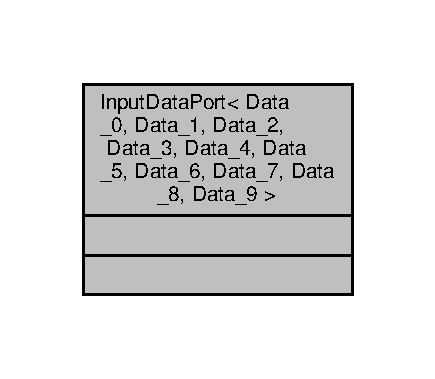
\includegraphics[width=209pt]{classInputDataPort__coll__graph}
\end{center}
\end{figure}


\subsection{상세한 설명}
\subsubsection*{template$<$typename Data\+\_\+0, typename Data\+\_\+1, typename Data\+\_\+2, typename Data\+\_\+3, typename Data\+\_\+4, typename Data\+\_\+5, typename Data\+\_\+6, typename Data\+\_\+7, typename Data\+\_\+8, typename Data\+\_\+9$>$\\*
class Input\+Data\+Port$<$ Data\+\_\+0, Data\+\_\+1, Data\+\_\+2, Data\+\_\+3, Data\+\_\+4, Data\+\_\+5, Data\+\_\+6, Data\+\_\+7, Data\+\_\+8, Data\+\_\+9 $>$}



Base\+\_\+cell\+\_\+temp.\+cpp 파일의 11 번째 라인에서 정의되었습니다.



이 클래스에 대한 문서화 페이지는 다음의 파일로부터 생성되었습니다.\+:\begin{DoxyCompactItemize}
\item 
src/\hyperlink{Base__cell__temp_8cpp}{Base\+\_\+cell\+\_\+temp.\+cpp}\end{DoxyCompactItemize}

\hypertarget{classInputDataPort__F}{}\section{Input\+Data\+Port\+\_\+F$<$ Data\+\_\+0, Data\+\_\+1, Data\+\_\+2, Data\+\_\+3, Data\+\_\+4, Data\+\_\+5, Data\+\_\+6, Data\+\_\+7, Data\+\_\+8, Data\+\_\+9 $>$}
\label{classInputDataPort__F}\index{Input\+Data\+Port\+\_\+\+F$<$ Data\+\_\+0, Data\+\_\+1, Data\+\_\+2, Data\+\_\+3, Data\+\_\+4, Data\+\_\+5, Data\+\_\+6, Data\+\_\+7, Data\+\_\+8, Data\+\_\+9 $>$@{Input\+Data\+Port\+\_\+\+F$<$ Data\+\_\+0, Data\+\_\+1, Data\+\_\+2, Data\+\_\+3, Data\+\_\+4, Data\+\_\+5, Data\+\_\+6, Data\+\_\+7, Data\+\_\+8, Data\+\_\+9 $>$}}


Input\+Data\+Port\+\_\+F$<$ Data\+\_\+0, Data\+\_\+1, Data\+\_\+2, Data\+\_\+3, Data\+\_\+4, Data\+\_\+5, Data\+\_\+6, Data\+\_\+7, Data\+\_\+8, Data\+\_\+9 $>$에 대한 협력 다이어그램\+:\nopagebreak
\begin{figure}[H]
\begin{center}
\leavevmode
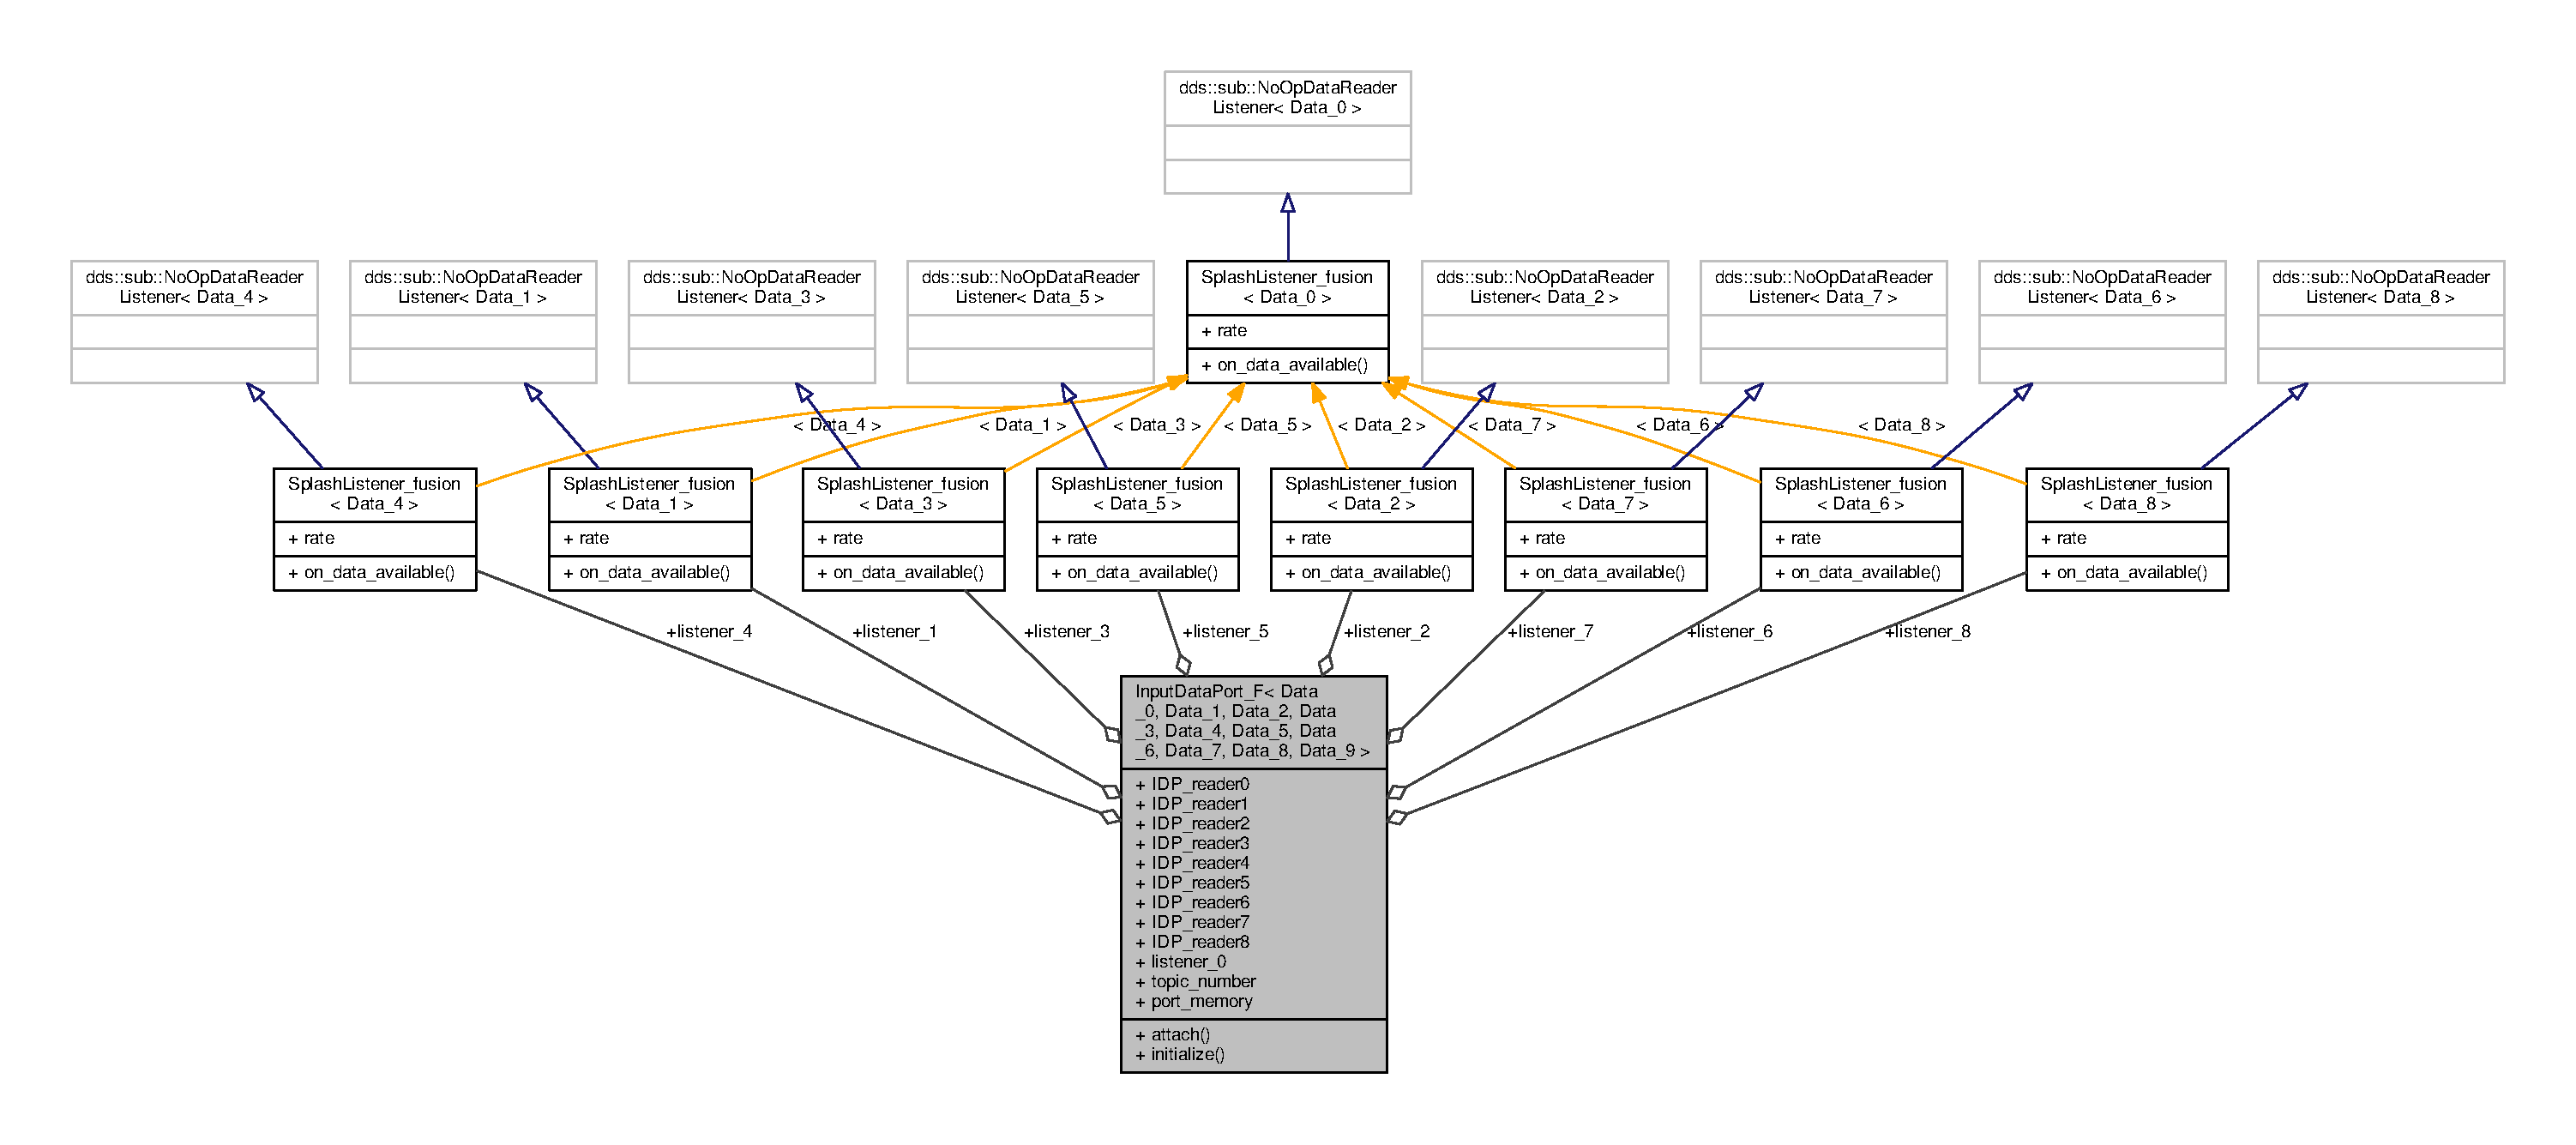
\includegraphics[width=350pt]{classInputDataPort__F__coll__graph}
\end{center}
\end{figure}
\subsection*{Public 멤버 함수}
\begin{DoxyCompactItemize}
\item 
int \hyperlink{classInputDataPort__F_a872e206ed74aca8952f23bcbb4973e58}{attach} (\hyperlink{classFusion__operator}{Fusion\+\_\+operator}$<$Data\+\_\+0, Data\+\_\+1, Data\+\_\+2, Data\+\_\+3, Data\+\_\+4, Data\+\_\+5, Data\+\_\+6, Data\+\_\+7, Data\+\_\+8, Data\+\_\+9 $>$ $\ast$, std\+::string, int, int)
\item 
void \hyperlink{classInputDataPort__F_a349a2f0ae2bf270a337e6db9e636b78b}{initialize} (double, void($\ast$)(), double, void($\ast$)(), bool, int)
\end{DoxyCompactItemize}
\subsection*{Public 속성}
\begin{DoxyCompactItemize}
\item 
dds\+::sub\+::\+Data\+Reader$<$ Data\+\_\+0 $>$ $\ast$ \hyperlink{classInputDataPort__F_a6b4b35818e400517815b7c6ba257f575}{I\+D\+P\+\_\+reader0}
\item 
dds\+::sub\+::\+Data\+Reader$<$ Data\+\_\+1 $>$ $\ast$ \hyperlink{classInputDataPort__F_a79b0bd4a5163911b5fc61610fdd9c0f2}{I\+D\+P\+\_\+reader1}
\item 
dds\+::sub\+::\+Data\+Reader$<$ Data\+\_\+2 $>$ $\ast$ \hyperlink{classInputDataPort__F_ae81ece0920bedb7e31fe559220a7aa3f}{I\+D\+P\+\_\+reader2}
\item 
dds\+::sub\+::\+Data\+Reader$<$ Data\+\_\+3 $>$ $\ast$ \hyperlink{classInputDataPort__F_a3d951f807fddce8487ad9b31586a4ba5}{I\+D\+P\+\_\+reader3}
\item 
dds\+::sub\+::\+Data\+Reader$<$ Data\+\_\+4 $>$ $\ast$ \hyperlink{classInputDataPort__F_a2257ff7fb24baade0c2f444b5a5605ab}{I\+D\+P\+\_\+reader4}
\item 
dds\+::sub\+::\+Data\+Reader$<$ Data\+\_\+5 $>$ $\ast$ \hyperlink{classInputDataPort__F_a5fd5d86cc8ddc3221b09f0c362c00b79}{I\+D\+P\+\_\+reader5}
\item 
dds\+::sub\+::\+Data\+Reader$<$ Data\+\_\+6 $>$ $\ast$ \hyperlink{classInputDataPort__F_a32834a466932265f79cf2b3bab07acd8}{I\+D\+P\+\_\+reader6}
\item 
dds\+::sub\+::\+Data\+Reader$<$ Data\+\_\+7 $>$ $\ast$ \hyperlink{classInputDataPort__F_ae04efc90dc8587b312b240d549399894}{I\+D\+P\+\_\+reader7}
\item 
dds\+::sub\+::\+Data\+Reader$<$ Data\+\_\+8 $>$ $\ast$ \hyperlink{classInputDataPort__F_a909a04c67500a9661ec84791b9739476}{I\+D\+P\+\_\+reader8}
\item 
\hyperlink{classSplashListener__fusion}{Splash\+Listener\+\_\+fusion}$<$ Data\+\_\+0 $>$ $\ast$ \hyperlink{classInputDataPort__F_a1b73682b2bc71e7b9f85be1d6e5655da}{listener\+\_\+0}
\item 
\hyperlink{classSplashListener__fusion}{Splash\+Listener\+\_\+fusion}$<$ Data\+\_\+1 $>$ $\ast$ \hyperlink{classInputDataPort__F_a3c5532c1682ea7ce7aef4b3f50923f51}{listener\+\_\+1}
\item 
\hyperlink{classSplashListener__fusion}{Splash\+Listener\+\_\+fusion}$<$ Data\+\_\+2 $>$ $\ast$ \hyperlink{classInputDataPort__F_ac54eb8cc1b48c4e414add9fd1fed9725}{listener\+\_\+2}
\item 
\hyperlink{classSplashListener__fusion}{Splash\+Listener\+\_\+fusion}$<$ Data\+\_\+3 $>$ $\ast$ \hyperlink{classInputDataPort__F_af34ec96b45b9f778eebac6e72901901a}{listener\+\_\+3}
\item 
\hyperlink{classSplashListener__fusion}{Splash\+Listener\+\_\+fusion}$<$ Data\+\_\+4 $>$ $\ast$ \hyperlink{classInputDataPort__F_a2306c92d87224281fbe8af0c1f4a7b1a}{listener\+\_\+4}
\item 
\hyperlink{classSplashListener__fusion}{Splash\+Listener\+\_\+fusion}$<$ Data\+\_\+5 $>$ $\ast$ \hyperlink{classInputDataPort__F_aba79969b7956c70a2f2101fc55370447}{listener\+\_\+5}
\item 
\hyperlink{classSplashListener__fusion}{Splash\+Listener\+\_\+fusion}$<$ Data\+\_\+6 $>$ $\ast$ \hyperlink{classInputDataPort__F_a99b57cc9e7aadd5bef83a3dc96eb7680}{listener\+\_\+6}
\item 
\hyperlink{classSplashListener__fusion}{Splash\+Listener\+\_\+fusion}$<$ Data\+\_\+7 $>$ $\ast$ \hyperlink{classInputDataPort__F_af2b7e4cfb20ef4fb3e945e32d8792fd2}{listener\+\_\+7}
\item 
\hyperlink{classSplashListener__fusion}{Splash\+Listener\+\_\+fusion}$<$ Data\+\_\+8 $>$ $\ast$ \hyperlink{classInputDataPort__F_a8af8e7aa880396f0945052e5cfc1985b}{listener\+\_\+8}
\item 
int \hyperlink{classInputDataPort__F_aa3975f3abd074e8fb18f34a4806d1f85}{topic\+\_\+number} =0
\item 
void $\ast$ \hyperlink{classInputDataPort__F_ab79e16d625d49923eb7e3864f8b2359e}{port\+\_\+memory}
\end{DoxyCompactItemize}


\subsection{상세한 설명}
\subsubsection*{template$<$typename Data\+\_\+0, typename Data\+\_\+1, typename Data\+\_\+2, typename Data\+\_\+3, typename Data\+\_\+4, typename Data\+\_\+5, typename Data\+\_\+6, typename Data\+\_\+7, typename Data\+\_\+8, typename Data\+\_\+9$>$\\*
class Input\+Data\+Port\+\_\+\+F$<$ Data\+\_\+0, Data\+\_\+1, Data\+\_\+2, Data\+\_\+3, Data\+\_\+4, Data\+\_\+5, Data\+\_\+6, Data\+\_\+7, Data\+\_\+8, Data\+\_\+9 $>$}



Fusion\+\_\+operator.\+cpp 파일의 14 번째 라인에서 정의되었습니다.



\subsection{멤버 함수 문서화}
\index{Input\+Data\+Port\+\_\+F@{Input\+Data\+Port\+\_\+F}!attach@{attach}}
\index{attach@{attach}!Input\+Data\+Port\+\_\+F@{Input\+Data\+Port\+\_\+F}}
\subsubsection[{\texorpdfstring{attach(\+Fusion\+\_\+operator$<$\+Data\+\_\+0, Data\+\_\+1, Data\+\_\+2, Data\+\_\+3, Data\+\_\+4, Data\+\_\+5, Data\+\_\+6, Data\+\_\+7, Data\+\_\+8, Data\+\_\+9 $>$ $\ast$, std\+::string, int, int)}{attach(Fusion_operator<Data_0, Data_1, Data_2, Data_3, Data_4, Data_5, Data_6, Data_7, Data_8, Data_9 > *, std::string, int, int)}}]{\setlength{\rightskip}{0pt plus 5cm}template$<$typename Data\+\_\+0 , typename Data\+\_\+1 , typename Data\+\_\+2 , typename Data\+\_\+3 , typename Data\+\_\+4 , typename Data\+\_\+5 , typename Data\+\_\+6 , typename Data\+\_\+7 , typename Data\+\_\+8 , typename Data\+\_\+9 $>$ int {\bf Input\+Data\+Port\+\_\+F}$<$ Data\+\_\+0, Data\+\_\+1, Data\+\_\+2, Data\+\_\+3, Data\+\_\+4, Data\+\_\+5, Data\+\_\+6, Data\+\_\+7, Data\+\_\+8, Data\+\_\+9 $>$\+::attach (
\begin{DoxyParamCaption}
\item[{{\bf Fusion\+\_\+operator}$<$Data\+\_\+0, Data\+\_\+1, Data\+\_\+2, Data\+\_\+3, Data\+\_\+4, Data\+\_\+5, Data\+\_\+6, Data\+\_\+7, Data\+\_\+8, Data\+\_\+9 $>$ $\ast$}]{PB, }
\item[{std\+::string}]{topic, }
\item[{int}]{topic\+\_\+number, }
\item[{int}]{mandatory}
\end{DoxyParamCaption}
)}\hypertarget{classInputDataPort__F_a872e206ed74aca8952f23bcbb4973e58}{}\label{classInputDataPort__F_a872e206ed74aca8952f23bcbb4973e58}


Fusion\+\_\+operator.\+cpp 파일의 236 번째 라인에서 정의되었습니다.



다음을 참조함 \+:  Fusion\+\_\+operator$<$ Data\+\_\+0, Data\+\_\+1, Data\+\_\+2, Data\+\_\+3, Data\+\_\+4, Data\+\_\+5, Data\+\_\+6, Data\+\_\+7, Data\+\_\+8, Data\+\_\+9 $>$\+::connected\+\_\+ports, Fusion\+\_\+operator$<$ Data\+\_\+0, Data\+\_\+1, Data\+\_\+2, Data\+\_\+3, Data\+\_\+4, Data\+\_\+5, Data\+\_\+6, Data\+\_\+7, Data\+\_\+8, Data\+\_\+9 $>$\+::\+I\+D\+P0, Fusion\+\_\+operator$<$ Data\+\_\+0, Data\+\_\+1, Data\+\_\+2, Data\+\_\+3, Data\+\_\+4, Data\+\_\+5, Data\+\_\+6, Data\+\_\+7, Data\+\_\+8, Data\+\_\+9 $>$\+::\+I\+D\+P1, Fusion\+\_\+operator$<$ Data\+\_\+0, Data\+\_\+1, Data\+\_\+2, Data\+\_\+3, Data\+\_\+4, Data\+\_\+5, Data\+\_\+6, Data\+\_\+7, Data\+\_\+8, Data\+\_\+9 $>$\+::\+I\+D\+P2, Fusion\+\_\+operator$<$ Data\+\_\+0, Data\+\_\+1, Data\+\_\+2, Data\+\_\+3, Data\+\_\+4, Data\+\_\+5, Data\+\_\+6, Data\+\_\+7, Data\+\_\+8, Data\+\_\+9 $>$\+::\+I\+D\+P3, Fusion\+\_\+operator$<$ Data\+\_\+0, Data\+\_\+1, Data\+\_\+2, Data\+\_\+3, Data\+\_\+4, Data\+\_\+5, Data\+\_\+6, Data\+\_\+7, Data\+\_\+8, Data\+\_\+9 $>$\+::\+I\+D\+P4, Fusion\+\_\+operator$<$ Data\+\_\+0, Data\+\_\+1, Data\+\_\+2, Data\+\_\+3, Data\+\_\+4, Data\+\_\+5, Data\+\_\+6, Data\+\_\+7, Data\+\_\+8, Data\+\_\+9 $>$\+::\+I\+D\+P5, Fusion\+\_\+operator$<$ Data\+\_\+0, Data\+\_\+1, Data\+\_\+2, Data\+\_\+3, Data\+\_\+4, Data\+\_\+5, Data\+\_\+6, Data\+\_\+7, Data\+\_\+8, Data\+\_\+9 $>$\+::\+I\+D\+P6, Fusion\+\_\+operator$<$ Data\+\_\+0, Data\+\_\+1, Data\+\_\+2, Data\+\_\+3, Data\+\_\+4, Data\+\_\+5, Data\+\_\+6, Data\+\_\+7, Data\+\_\+8, Data\+\_\+9 $>$\+::\+I\+D\+P7, Fusion\+\_\+operator$<$ Data\+\_\+0, Data\+\_\+1, Data\+\_\+2, Data\+\_\+3, Data\+\_\+4, Data\+\_\+5, Data\+\_\+6, Data\+\_\+7, Data\+\_\+8, Data\+\_\+9 $>$\+::\+I\+D\+P8, Fusion\+\_\+operator$<$ Data\+\_\+0, Data\+\_\+1, Data\+\_\+2, Data\+\_\+3, Data\+\_\+4, Data\+\_\+5, Data\+\_\+6, Data\+\_\+7, Data\+\_\+8, Data\+\_\+9 $>$\+::mandport, Fusion\+\_\+operator$<$ Data\+\_\+0, Data\+\_\+1, Data\+\_\+2, Data\+\_\+3, Data\+\_\+4, Data\+\_\+5, Data\+\_\+6, Data\+\_\+7, Data\+\_\+8, Data\+\_\+9 $>$\+::topic0, Fusion\+\_\+operator$<$ Data\+\_\+0, Data\+\_\+1, Data\+\_\+2, Data\+\_\+3, Data\+\_\+4, Data\+\_\+5, Data\+\_\+6, Data\+\_\+7, Data\+\_\+8, Data\+\_\+9 $>$\+::topic1, Fusion\+\_\+operator$<$ Data\+\_\+0, Data\+\_\+1, Data\+\_\+2, Data\+\_\+3, Data\+\_\+4, Data\+\_\+5, Data\+\_\+6, Data\+\_\+7, Data\+\_\+8, Data\+\_\+9 $>$\+::topic2, Fusion\+\_\+operator$<$ Data\+\_\+0, Data\+\_\+1, Data\+\_\+2, Data\+\_\+3, Data\+\_\+4, Data\+\_\+5, Data\+\_\+6, Data\+\_\+7, Data\+\_\+8, Data\+\_\+9 $>$\+::topic3, Fusion\+\_\+operator$<$ Data\+\_\+0, Data\+\_\+1, Data\+\_\+2, Data\+\_\+3, Data\+\_\+4, Data\+\_\+5, Data\+\_\+6, Data\+\_\+7, Data\+\_\+8, Data\+\_\+9 $>$\+::topic4, Fusion\+\_\+operator$<$ Data\+\_\+0, Data\+\_\+1, Data\+\_\+2, Data\+\_\+3, Data\+\_\+4, Data\+\_\+5, Data\+\_\+6, Data\+\_\+7, Data\+\_\+8, Data\+\_\+9 $>$\+::topic5, Fusion\+\_\+operator$<$ Data\+\_\+0, Data\+\_\+1, Data\+\_\+2, Data\+\_\+3, Data\+\_\+4, Data\+\_\+5, Data\+\_\+6, Data\+\_\+7, Data\+\_\+8, Data\+\_\+9 $>$\+::topic6, Fusion\+\_\+operator$<$ Data\+\_\+0, Data\+\_\+1, Data\+\_\+2, Data\+\_\+3, Data\+\_\+4, Data\+\_\+5, Data\+\_\+6, Data\+\_\+7, Data\+\_\+8, Data\+\_\+9 $>$\+::topic7, Fusion\+\_\+operator$<$ Data\+\_\+0, Data\+\_\+1, Data\+\_\+2, Data\+\_\+3, Data\+\_\+4, Data\+\_\+5, Data\+\_\+6, Data\+\_\+7, Data\+\_\+8, Data\+\_\+9 $>$\+::topic8, Fusion\+\_\+operator$<$ Data\+\_\+0, Data\+\_\+1, Data\+\_\+2, Data\+\_\+3, Data\+\_\+4, Data\+\_\+5, Data\+\_\+6, Data\+\_\+7, Data\+\_\+8, Data\+\_\+9 $>$\+::ws\+\_\+0, Fusion\+\_\+operator$<$ Data\+\_\+0, Data\+\_\+1, Data\+\_\+2, Data\+\_\+3, Data\+\_\+4, Data\+\_\+5, Data\+\_\+6, Data\+\_\+7, Data\+\_\+8, Data\+\_\+9 $>$\+::ws\+\_\+1, Fusion\+\_\+operator$<$ Data\+\_\+0, Data\+\_\+1, Data\+\_\+2, Data\+\_\+3, Data\+\_\+4, Data\+\_\+5, Data\+\_\+6, Data\+\_\+7, Data\+\_\+8, Data\+\_\+9 $>$\+::ws\+\_\+2, Fusion\+\_\+operator$<$ Data\+\_\+0, Data\+\_\+1, Data\+\_\+2, Data\+\_\+3, Data\+\_\+4, Data\+\_\+5, Data\+\_\+6, Data\+\_\+7, Data\+\_\+8, Data\+\_\+9 $>$\+::ws\+\_\+3, Fusion\+\_\+operator$<$ Data\+\_\+0, Data\+\_\+1, Data\+\_\+2, Data\+\_\+3, Data\+\_\+4, Data\+\_\+5, Data\+\_\+6, Data\+\_\+7, Data\+\_\+8, Data\+\_\+9 $>$\+::ws\+\_\+4, Fusion\+\_\+operator$<$ Data\+\_\+0, Data\+\_\+1, Data\+\_\+2, Data\+\_\+3, Data\+\_\+4, Data\+\_\+5, Data\+\_\+6, Data\+\_\+7, Data\+\_\+8, Data\+\_\+9 $>$\+::ws\+\_\+5, Fusion\+\_\+operator$<$ Data\+\_\+0, Data\+\_\+1, Data\+\_\+2, Data\+\_\+3, Data\+\_\+4, Data\+\_\+5, Data\+\_\+6, Data\+\_\+7, Data\+\_\+8, Data\+\_\+9 $>$\+::ws\+\_\+6, Fusion\+\_\+operator$<$ Data\+\_\+0, Data\+\_\+1, Data\+\_\+2, Data\+\_\+3, Data\+\_\+4, Data\+\_\+5, Data\+\_\+6, Data\+\_\+7, Data\+\_\+8, Data\+\_\+9 $>$\+::ws\+\_\+7, Fusion\+\_\+operator$<$ Data\+\_\+0, Data\+\_\+1, Data\+\_\+2, Data\+\_\+3, Data\+\_\+4, Data\+\_\+5, Data\+\_\+6, Data\+\_\+7, Data\+\_\+8, Data\+\_\+9 $>$\+::ws\+\_\+8.

\index{Input\+Data\+Port\+\_\+F@{Input\+Data\+Port\+\_\+F}!initialize@{initialize}}
\index{initialize@{initialize}!Input\+Data\+Port\+\_\+F@{Input\+Data\+Port\+\_\+F}}
\subsubsection[{\texorpdfstring{initialize(double, void($\ast$)(), double, void($\ast$)(), bool, int)}{initialize(double, void(*)(), double, void(*)(), bool, int)}}]{\setlength{\rightskip}{0pt plus 5cm}template$<$typename Data\+\_\+0 , typename Data\+\_\+1 , typename Data\+\_\+2 , typename Data\+\_\+3 , typename Data\+\_\+4 , typename Data\+\_\+5 , typename Data\+\_\+6 , typename Data\+\_\+7 , typename Data\+\_\+8 , typename Data\+\_\+9 $>$ void {\bf Input\+Data\+Port\+\_\+F}$<$ Data\+\_\+0, Data\+\_\+1, Data\+\_\+2, Data\+\_\+3, Data\+\_\+4, Data\+\_\+5, Data\+\_\+6, Data\+\_\+7, Data\+\_\+8, Data\+\_\+9 $>$\+::initialize (
\begin{DoxyParamCaption}
\item[{double}]{rate, }
\item[{void($\ast$)()}]{rate\+\_\+handler, }
\item[{double}]{freshness, }
\item[{void($\ast$)()}]{freshness\+\_\+handler, }
\item[{bool}]{queueing, }
\item[{int}]{queue\+\_\+size}
\end{DoxyParamCaption}
)}\hypertarget{classInputDataPort__F_a349a2f0ae2bf270a337e6db9e636b78b}{}\label{classInputDataPort__F_a349a2f0ae2bf270a337e6db9e636b78b}


Fusion\+\_\+operator.\+cpp 파일의 446 번째 라인에서 정의되었습니다.



\subsection{멤버 데이타 문서화}
\index{Input\+Data\+Port\+\_\+F@{Input\+Data\+Port\+\_\+F}!I\+D\+P\+\_\+reader0@{I\+D\+P\+\_\+reader0}}
\index{I\+D\+P\+\_\+reader0@{I\+D\+P\+\_\+reader0}!Input\+Data\+Port\+\_\+F@{Input\+Data\+Port\+\_\+F}}
\subsubsection[{\texorpdfstring{I\+D\+P\+\_\+reader0}{IDP_reader0}}]{\setlength{\rightskip}{0pt plus 5cm}template$<$typename Data\+\_\+0 , typename Data\+\_\+1 , typename Data\+\_\+2 , typename Data\+\_\+3 , typename Data\+\_\+4 , typename Data\+\_\+5 , typename Data\+\_\+6 , typename Data\+\_\+7 , typename Data\+\_\+8 , typename Data\+\_\+9 $>$ dds\+::sub\+::\+Data\+Reader$<$Data\+\_\+0$>$$\ast$ {\bf Input\+Data\+Port\+\_\+F}$<$ Data\+\_\+0, Data\+\_\+1, Data\+\_\+2, Data\+\_\+3, Data\+\_\+4, Data\+\_\+5, Data\+\_\+6, Data\+\_\+7, Data\+\_\+8, Data\+\_\+9 $>$\+::I\+D\+P\+\_\+reader0}\hypertarget{classInputDataPort__F_a6b4b35818e400517815b7c6ba257f575}{}\label{classInputDataPort__F_a6b4b35818e400517815b7c6ba257f575}


Fusion\+\_\+operator.\+cpp 파일의 200 번째 라인에서 정의되었습니다.

\index{Input\+Data\+Port\+\_\+F@{Input\+Data\+Port\+\_\+F}!I\+D\+P\+\_\+reader1@{I\+D\+P\+\_\+reader1}}
\index{I\+D\+P\+\_\+reader1@{I\+D\+P\+\_\+reader1}!Input\+Data\+Port\+\_\+F@{Input\+Data\+Port\+\_\+F}}
\subsubsection[{\texorpdfstring{I\+D\+P\+\_\+reader1}{IDP_reader1}}]{\setlength{\rightskip}{0pt plus 5cm}template$<$typename Data\+\_\+0 , typename Data\+\_\+1 , typename Data\+\_\+2 , typename Data\+\_\+3 , typename Data\+\_\+4 , typename Data\+\_\+5 , typename Data\+\_\+6 , typename Data\+\_\+7 , typename Data\+\_\+8 , typename Data\+\_\+9 $>$ dds\+::sub\+::\+Data\+Reader$<$Data\+\_\+1$>$$\ast$ {\bf Input\+Data\+Port\+\_\+F}$<$ Data\+\_\+0, Data\+\_\+1, Data\+\_\+2, Data\+\_\+3, Data\+\_\+4, Data\+\_\+5, Data\+\_\+6, Data\+\_\+7, Data\+\_\+8, Data\+\_\+9 $>$\+::I\+D\+P\+\_\+reader1}\hypertarget{classInputDataPort__F_a79b0bd4a5163911b5fc61610fdd9c0f2}{}\label{classInputDataPort__F_a79b0bd4a5163911b5fc61610fdd9c0f2}


Fusion\+\_\+operator.\+cpp 파일의 201 번째 라인에서 정의되었습니다.

\index{Input\+Data\+Port\+\_\+F@{Input\+Data\+Port\+\_\+F}!I\+D\+P\+\_\+reader2@{I\+D\+P\+\_\+reader2}}
\index{I\+D\+P\+\_\+reader2@{I\+D\+P\+\_\+reader2}!Input\+Data\+Port\+\_\+F@{Input\+Data\+Port\+\_\+F}}
\subsubsection[{\texorpdfstring{I\+D\+P\+\_\+reader2}{IDP_reader2}}]{\setlength{\rightskip}{0pt plus 5cm}template$<$typename Data\+\_\+0 , typename Data\+\_\+1 , typename Data\+\_\+2 , typename Data\+\_\+3 , typename Data\+\_\+4 , typename Data\+\_\+5 , typename Data\+\_\+6 , typename Data\+\_\+7 , typename Data\+\_\+8 , typename Data\+\_\+9 $>$ dds\+::sub\+::\+Data\+Reader$<$Data\+\_\+2$>$$\ast$ {\bf Input\+Data\+Port\+\_\+F}$<$ Data\+\_\+0, Data\+\_\+1, Data\+\_\+2, Data\+\_\+3, Data\+\_\+4, Data\+\_\+5, Data\+\_\+6, Data\+\_\+7, Data\+\_\+8, Data\+\_\+9 $>$\+::I\+D\+P\+\_\+reader2}\hypertarget{classInputDataPort__F_ae81ece0920bedb7e31fe559220a7aa3f}{}\label{classInputDataPort__F_ae81ece0920bedb7e31fe559220a7aa3f}


Fusion\+\_\+operator.\+cpp 파일의 202 번째 라인에서 정의되었습니다.

\index{Input\+Data\+Port\+\_\+F@{Input\+Data\+Port\+\_\+F}!I\+D\+P\+\_\+reader3@{I\+D\+P\+\_\+reader3}}
\index{I\+D\+P\+\_\+reader3@{I\+D\+P\+\_\+reader3}!Input\+Data\+Port\+\_\+F@{Input\+Data\+Port\+\_\+F}}
\subsubsection[{\texorpdfstring{I\+D\+P\+\_\+reader3}{IDP_reader3}}]{\setlength{\rightskip}{0pt plus 5cm}template$<$typename Data\+\_\+0 , typename Data\+\_\+1 , typename Data\+\_\+2 , typename Data\+\_\+3 , typename Data\+\_\+4 , typename Data\+\_\+5 , typename Data\+\_\+6 , typename Data\+\_\+7 , typename Data\+\_\+8 , typename Data\+\_\+9 $>$ dds\+::sub\+::\+Data\+Reader$<$Data\+\_\+3$>$$\ast$ {\bf Input\+Data\+Port\+\_\+F}$<$ Data\+\_\+0, Data\+\_\+1, Data\+\_\+2, Data\+\_\+3, Data\+\_\+4, Data\+\_\+5, Data\+\_\+6, Data\+\_\+7, Data\+\_\+8, Data\+\_\+9 $>$\+::I\+D\+P\+\_\+reader3}\hypertarget{classInputDataPort__F_a3d951f807fddce8487ad9b31586a4ba5}{}\label{classInputDataPort__F_a3d951f807fddce8487ad9b31586a4ba5}


Fusion\+\_\+operator.\+cpp 파일의 203 번째 라인에서 정의되었습니다.

\index{Input\+Data\+Port\+\_\+F@{Input\+Data\+Port\+\_\+F}!I\+D\+P\+\_\+reader4@{I\+D\+P\+\_\+reader4}}
\index{I\+D\+P\+\_\+reader4@{I\+D\+P\+\_\+reader4}!Input\+Data\+Port\+\_\+F@{Input\+Data\+Port\+\_\+F}}
\subsubsection[{\texorpdfstring{I\+D\+P\+\_\+reader4}{IDP_reader4}}]{\setlength{\rightskip}{0pt plus 5cm}template$<$typename Data\+\_\+0 , typename Data\+\_\+1 , typename Data\+\_\+2 , typename Data\+\_\+3 , typename Data\+\_\+4 , typename Data\+\_\+5 , typename Data\+\_\+6 , typename Data\+\_\+7 , typename Data\+\_\+8 , typename Data\+\_\+9 $>$ dds\+::sub\+::\+Data\+Reader$<$Data\+\_\+4$>$$\ast$ {\bf Input\+Data\+Port\+\_\+F}$<$ Data\+\_\+0, Data\+\_\+1, Data\+\_\+2, Data\+\_\+3, Data\+\_\+4, Data\+\_\+5, Data\+\_\+6, Data\+\_\+7, Data\+\_\+8, Data\+\_\+9 $>$\+::I\+D\+P\+\_\+reader4}\hypertarget{classInputDataPort__F_a2257ff7fb24baade0c2f444b5a5605ab}{}\label{classInputDataPort__F_a2257ff7fb24baade0c2f444b5a5605ab}


Fusion\+\_\+operator.\+cpp 파일의 204 번째 라인에서 정의되었습니다.

\index{Input\+Data\+Port\+\_\+F@{Input\+Data\+Port\+\_\+F}!I\+D\+P\+\_\+reader5@{I\+D\+P\+\_\+reader5}}
\index{I\+D\+P\+\_\+reader5@{I\+D\+P\+\_\+reader5}!Input\+Data\+Port\+\_\+F@{Input\+Data\+Port\+\_\+F}}
\subsubsection[{\texorpdfstring{I\+D\+P\+\_\+reader5}{IDP_reader5}}]{\setlength{\rightskip}{0pt plus 5cm}template$<$typename Data\+\_\+0 , typename Data\+\_\+1 , typename Data\+\_\+2 , typename Data\+\_\+3 , typename Data\+\_\+4 , typename Data\+\_\+5 , typename Data\+\_\+6 , typename Data\+\_\+7 , typename Data\+\_\+8 , typename Data\+\_\+9 $>$ dds\+::sub\+::\+Data\+Reader$<$Data\+\_\+5$>$$\ast$ {\bf Input\+Data\+Port\+\_\+F}$<$ Data\+\_\+0, Data\+\_\+1, Data\+\_\+2, Data\+\_\+3, Data\+\_\+4, Data\+\_\+5, Data\+\_\+6, Data\+\_\+7, Data\+\_\+8, Data\+\_\+9 $>$\+::I\+D\+P\+\_\+reader5}\hypertarget{classInputDataPort__F_a5fd5d86cc8ddc3221b09f0c362c00b79}{}\label{classInputDataPort__F_a5fd5d86cc8ddc3221b09f0c362c00b79}


Fusion\+\_\+operator.\+cpp 파일의 205 번째 라인에서 정의되었습니다.

\index{Input\+Data\+Port\+\_\+F@{Input\+Data\+Port\+\_\+F}!I\+D\+P\+\_\+reader6@{I\+D\+P\+\_\+reader6}}
\index{I\+D\+P\+\_\+reader6@{I\+D\+P\+\_\+reader6}!Input\+Data\+Port\+\_\+F@{Input\+Data\+Port\+\_\+F}}
\subsubsection[{\texorpdfstring{I\+D\+P\+\_\+reader6}{IDP_reader6}}]{\setlength{\rightskip}{0pt plus 5cm}template$<$typename Data\+\_\+0 , typename Data\+\_\+1 , typename Data\+\_\+2 , typename Data\+\_\+3 , typename Data\+\_\+4 , typename Data\+\_\+5 , typename Data\+\_\+6 , typename Data\+\_\+7 , typename Data\+\_\+8 , typename Data\+\_\+9 $>$ dds\+::sub\+::\+Data\+Reader$<$Data\+\_\+6$>$$\ast$ {\bf Input\+Data\+Port\+\_\+F}$<$ Data\+\_\+0, Data\+\_\+1, Data\+\_\+2, Data\+\_\+3, Data\+\_\+4, Data\+\_\+5, Data\+\_\+6, Data\+\_\+7, Data\+\_\+8, Data\+\_\+9 $>$\+::I\+D\+P\+\_\+reader6}\hypertarget{classInputDataPort__F_a32834a466932265f79cf2b3bab07acd8}{}\label{classInputDataPort__F_a32834a466932265f79cf2b3bab07acd8}


Fusion\+\_\+operator.\+cpp 파일의 206 번째 라인에서 정의되었습니다.

\index{Input\+Data\+Port\+\_\+F@{Input\+Data\+Port\+\_\+F}!I\+D\+P\+\_\+reader7@{I\+D\+P\+\_\+reader7}}
\index{I\+D\+P\+\_\+reader7@{I\+D\+P\+\_\+reader7}!Input\+Data\+Port\+\_\+F@{Input\+Data\+Port\+\_\+F}}
\subsubsection[{\texorpdfstring{I\+D\+P\+\_\+reader7}{IDP_reader7}}]{\setlength{\rightskip}{0pt plus 5cm}template$<$typename Data\+\_\+0 , typename Data\+\_\+1 , typename Data\+\_\+2 , typename Data\+\_\+3 , typename Data\+\_\+4 , typename Data\+\_\+5 , typename Data\+\_\+6 , typename Data\+\_\+7 , typename Data\+\_\+8 , typename Data\+\_\+9 $>$ dds\+::sub\+::\+Data\+Reader$<$Data\+\_\+7$>$$\ast$ {\bf Input\+Data\+Port\+\_\+F}$<$ Data\+\_\+0, Data\+\_\+1, Data\+\_\+2, Data\+\_\+3, Data\+\_\+4, Data\+\_\+5, Data\+\_\+6, Data\+\_\+7, Data\+\_\+8, Data\+\_\+9 $>$\+::I\+D\+P\+\_\+reader7}\hypertarget{classInputDataPort__F_ae04efc90dc8587b312b240d549399894}{}\label{classInputDataPort__F_ae04efc90dc8587b312b240d549399894}


Fusion\+\_\+operator.\+cpp 파일의 207 번째 라인에서 정의되었습니다.

\index{Input\+Data\+Port\+\_\+F@{Input\+Data\+Port\+\_\+F}!I\+D\+P\+\_\+reader8@{I\+D\+P\+\_\+reader8}}
\index{I\+D\+P\+\_\+reader8@{I\+D\+P\+\_\+reader8}!Input\+Data\+Port\+\_\+F@{Input\+Data\+Port\+\_\+F}}
\subsubsection[{\texorpdfstring{I\+D\+P\+\_\+reader8}{IDP_reader8}}]{\setlength{\rightskip}{0pt plus 5cm}template$<$typename Data\+\_\+0 , typename Data\+\_\+1 , typename Data\+\_\+2 , typename Data\+\_\+3 , typename Data\+\_\+4 , typename Data\+\_\+5 , typename Data\+\_\+6 , typename Data\+\_\+7 , typename Data\+\_\+8 , typename Data\+\_\+9 $>$ dds\+::sub\+::\+Data\+Reader$<$Data\+\_\+8$>$$\ast$ {\bf Input\+Data\+Port\+\_\+F}$<$ Data\+\_\+0, Data\+\_\+1, Data\+\_\+2, Data\+\_\+3, Data\+\_\+4, Data\+\_\+5, Data\+\_\+6, Data\+\_\+7, Data\+\_\+8, Data\+\_\+9 $>$\+::I\+D\+P\+\_\+reader8}\hypertarget{classInputDataPort__F_a909a04c67500a9661ec84791b9739476}{}\label{classInputDataPort__F_a909a04c67500a9661ec84791b9739476}


Fusion\+\_\+operator.\+cpp 파일의 208 번째 라인에서 정의되었습니다.

\index{Input\+Data\+Port\+\_\+F@{Input\+Data\+Port\+\_\+F}!listener\+\_\+0@{listener\+\_\+0}}
\index{listener\+\_\+0@{listener\+\_\+0}!Input\+Data\+Port\+\_\+F@{Input\+Data\+Port\+\_\+F}}
\subsubsection[{\texorpdfstring{listener\+\_\+0}{listener_0}}]{\setlength{\rightskip}{0pt plus 5cm}template$<$typename Data\+\_\+0 , typename Data\+\_\+1 , typename Data\+\_\+2 , typename Data\+\_\+3 , typename Data\+\_\+4 , typename Data\+\_\+5 , typename Data\+\_\+6 , typename Data\+\_\+7 , typename Data\+\_\+8 , typename Data\+\_\+9 $>$ {\bf Splash\+Listener\+\_\+fusion}$<$Data\+\_\+0$>$$\ast$ {\bf Input\+Data\+Port\+\_\+F}$<$ Data\+\_\+0, Data\+\_\+1, Data\+\_\+2, Data\+\_\+3, Data\+\_\+4, Data\+\_\+5, Data\+\_\+6, Data\+\_\+7, Data\+\_\+8, Data\+\_\+9 $>$\+::listener\+\_\+0}\hypertarget{classInputDataPort__F_a1b73682b2bc71e7b9f85be1d6e5655da}{}\label{classInputDataPort__F_a1b73682b2bc71e7b9f85be1d6e5655da}


Fusion\+\_\+operator.\+cpp 파일의 211 번째 라인에서 정의되었습니다.

\index{Input\+Data\+Port\+\_\+F@{Input\+Data\+Port\+\_\+F}!listener\+\_\+1@{listener\+\_\+1}}
\index{listener\+\_\+1@{listener\+\_\+1}!Input\+Data\+Port\+\_\+F@{Input\+Data\+Port\+\_\+F}}
\subsubsection[{\texorpdfstring{listener\+\_\+1}{listener_1}}]{\setlength{\rightskip}{0pt plus 5cm}template$<$typename Data\+\_\+0 , typename Data\+\_\+1 , typename Data\+\_\+2 , typename Data\+\_\+3 , typename Data\+\_\+4 , typename Data\+\_\+5 , typename Data\+\_\+6 , typename Data\+\_\+7 , typename Data\+\_\+8 , typename Data\+\_\+9 $>$ {\bf Splash\+Listener\+\_\+fusion}$<$Data\+\_\+1$>$$\ast$ {\bf Input\+Data\+Port\+\_\+F}$<$ Data\+\_\+0, Data\+\_\+1, Data\+\_\+2, Data\+\_\+3, Data\+\_\+4, Data\+\_\+5, Data\+\_\+6, Data\+\_\+7, Data\+\_\+8, Data\+\_\+9 $>$\+::listener\+\_\+1}\hypertarget{classInputDataPort__F_a3c5532c1682ea7ce7aef4b3f50923f51}{}\label{classInputDataPort__F_a3c5532c1682ea7ce7aef4b3f50923f51}


Fusion\+\_\+operator.\+cpp 파일의 212 번째 라인에서 정의되었습니다.

\index{Input\+Data\+Port\+\_\+F@{Input\+Data\+Port\+\_\+F}!listener\+\_\+2@{listener\+\_\+2}}
\index{listener\+\_\+2@{listener\+\_\+2}!Input\+Data\+Port\+\_\+F@{Input\+Data\+Port\+\_\+F}}
\subsubsection[{\texorpdfstring{listener\+\_\+2}{listener_2}}]{\setlength{\rightskip}{0pt plus 5cm}template$<$typename Data\+\_\+0 , typename Data\+\_\+1 , typename Data\+\_\+2 , typename Data\+\_\+3 , typename Data\+\_\+4 , typename Data\+\_\+5 , typename Data\+\_\+6 , typename Data\+\_\+7 , typename Data\+\_\+8 , typename Data\+\_\+9 $>$ {\bf Splash\+Listener\+\_\+fusion}$<$Data\+\_\+2$>$$\ast$ {\bf Input\+Data\+Port\+\_\+F}$<$ Data\+\_\+0, Data\+\_\+1, Data\+\_\+2, Data\+\_\+3, Data\+\_\+4, Data\+\_\+5, Data\+\_\+6, Data\+\_\+7, Data\+\_\+8, Data\+\_\+9 $>$\+::listener\+\_\+2}\hypertarget{classInputDataPort__F_ac54eb8cc1b48c4e414add9fd1fed9725}{}\label{classInputDataPort__F_ac54eb8cc1b48c4e414add9fd1fed9725}


Fusion\+\_\+operator.\+cpp 파일의 213 번째 라인에서 정의되었습니다.

\index{Input\+Data\+Port\+\_\+F@{Input\+Data\+Port\+\_\+F}!listener\+\_\+3@{listener\+\_\+3}}
\index{listener\+\_\+3@{listener\+\_\+3}!Input\+Data\+Port\+\_\+F@{Input\+Data\+Port\+\_\+F}}
\subsubsection[{\texorpdfstring{listener\+\_\+3}{listener_3}}]{\setlength{\rightskip}{0pt plus 5cm}template$<$typename Data\+\_\+0 , typename Data\+\_\+1 , typename Data\+\_\+2 , typename Data\+\_\+3 , typename Data\+\_\+4 , typename Data\+\_\+5 , typename Data\+\_\+6 , typename Data\+\_\+7 , typename Data\+\_\+8 , typename Data\+\_\+9 $>$ {\bf Splash\+Listener\+\_\+fusion}$<$Data\+\_\+3$>$$\ast$ {\bf Input\+Data\+Port\+\_\+F}$<$ Data\+\_\+0, Data\+\_\+1, Data\+\_\+2, Data\+\_\+3, Data\+\_\+4, Data\+\_\+5, Data\+\_\+6, Data\+\_\+7, Data\+\_\+8, Data\+\_\+9 $>$\+::listener\+\_\+3}\hypertarget{classInputDataPort__F_af34ec96b45b9f778eebac6e72901901a}{}\label{classInputDataPort__F_af34ec96b45b9f778eebac6e72901901a}


Fusion\+\_\+operator.\+cpp 파일의 214 번째 라인에서 정의되었습니다.

\index{Input\+Data\+Port\+\_\+F@{Input\+Data\+Port\+\_\+F}!listener\+\_\+4@{listener\+\_\+4}}
\index{listener\+\_\+4@{listener\+\_\+4}!Input\+Data\+Port\+\_\+F@{Input\+Data\+Port\+\_\+F}}
\subsubsection[{\texorpdfstring{listener\+\_\+4}{listener_4}}]{\setlength{\rightskip}{0pt plus 5cm}template$<$typename Data\+\_\+0 , typename Data\+\_\+1 , typename Data\+\_\+2 , typename Data\+\_\+3 , typename Data\+\_\+4 , typename Data\+\_\+5 , typename Data\+\_\+6 , typename Data\+\_\+7 , typename Data\+\_\+8 , typename Data\+\_\+9 $>$ {\bf Splash\+Listener\+\_\+fusion}$<$Data\+\_\+4$>$$\ast$ {\bf Input\+Data\+Port\+\_\+F}$<$ Data\+\_\+0, Data\+\_\+1, Data\+\_\+2, Data\+\_\+3, Data\+\_\+4, Data\+\_\+5, Data\+\_\+6, Data\+\_\+7, Data\+\_\+8, Data\+\_\+9 $>$\+::listener\+\_\+4}\hypertarget{classInputDataPort__F_a2306c92d87224281fbe8af0c1f4a7b1a}{}\label{classInputDataPort__F_a2306c92d87224281fbe8af0c1f4a7b1a}


Fusion\+\_\+operator.\+cpp 파일의 215 번째 라인에서 정의되었습니다.

\index{Input\+Data\+Port\+\_\+F@{Input\+Data\+Port\+\_\+F}!listener\+\_\+5@{listener\+\_\+5}}
\index{listener\+\_\+5@{listener\+\_\+5}!Input\+Data\+Port\+\_\+F@{Input\+Data\+Port\+\_\+F}}
\subsubsection[{\texorpdfstring{listener\+\_\+5}{listener_5}}]{\setlength{\rightskip}{0pt plus 5cm}template$<$typename Data\+\_\+0 , typename Data\+\_\+1 , typename Data\+\_\+2 , typename Data\+\_\+3 , typename Data\+\_\+4 , typename Data\+\_\+5 , typename Data\+\_\+6 , typename Data\+\_\+7 , typename Data\+\_\+8 , typename Data\+\_\+9 $>$ {\bf Splash\+Listener\+\_\+fusion}$<$Data\+\_\+5$>$$\ast$ {\bf Input\+Data\+Port\+\_\+F}$<$ Data\+\_\+0, Data\+\_\+1, Data\+\_\+2, Data\+\_\+3, Data\+\_\+4, Data\+\_\+5, Data\+\_\+6, Data\+\_\+7, Data\+\_\+8, Data\+\_\+9 $>$\+::listener\+\_\+5}\hypertarget{classInputDataPort__F_aba79969b7956c70a2f2101fc55370447}{}\label{classInputDataPort__F_aba79969b7956c70a2f2101fc55370447}


Fusion\+\_\+operator.\+cpp 파일의 216 번째 라인에서 정의되었습니다.

\index{Input\+Data\+Port\+\_\+F@{Input\+Data\+Port\+\_\+F}!listener\+\_\+6@{listener\+\_\+6}}
\index{listener\+\_\+6@{listener\+\_\+6}!Input\+Data\+Port\+\_\+F@{Input\+Data\+Port\+\_\+F}}
\subsubsection[{\texorpdfstring{listener\+\_\+6}{listener_6}}]{\setlength{\rightskip}{0pt plus 5cm}template$<$typename Data\+\_\+0 , typename Data\+\_\+1 , typename Data\+\_\+2 , typename Data\+\_\+3 , typename Data\+\_\+4 , typename Data\+\_\+5 , typename Data\+\_\+6 , typename Data\+\_\+7 , typename Data\+\_\+8 , typename Data\+\_\+9 $>$ {\bf Splash\+Listener\+\_\+fusion}$<$Data\+\_\+6$>$$\ast$ {\bf Input\+Data\+Port\+\_\+F}$<$ Data\+\_\+0, Data\+\_\+1, Data\+\_\+2, Data\+\_\+3, Data\+\_\+4, Data\+\_\+5, Data\+\_\+6, Data\+\_\+7, Data\+\_\+8, Data\+\_\+9 $>$\+::listener\+\_\+6}\hypertarget{classInputDataPort__F_a99b57cc9e7aadd5bef83a3dc96eb7680}{}\label{classInputDataPort__F_a99b57cc9e7aadd5bef83a3dc96eb7680}


Fusion\+\_\+operator.\+cpp 파일의 217 번째 라인에서 정의되었습니다.

\index{Input\+Data\+Port\+\_\+F@{Input\+Data\+Port\+\_\+F}!listener\+\_\+7@{listener\+\_\+7}}
\index{listener\+\_\+7@{listener\+\_\+7}!Input\+Data\+Port\+\_\+F@{Input\+Data\+Port\+\_\+F}}
\subsubsection[{\texorpdfstring{listener\+\_\+7}{listener_7}}]{\setlength{\rightskip}{0pt plus 5cm}template$<$typename Data\+\_\+0 , typename Data\+\_\+1 , typename Data\+\_\+2 , typename Data\+\_\+3 , typename Data\+\_\+4 , typename Data\+\_\+5 , typename Data\+\_\+6 , typename Data\+\_\+7 , typename Data\+\_\+8 , typename Data\+\_\+9 $>$ {\bf Splash\+Listener\+\_\+fusion}$<$Data\+\_\+7$>$$\ast$ {\bf Input\+Data\+Port\+\_\+F}$<$ Data\+\_\+0, Data\+\_\+1, Data\+\_\+2, Data\+\_\+3, Data\+\_\+4, Data\+\_\+5, Data\+\_\+6, Data\+\_\+7, Data\+\_\+8, Data\+\_\+9 $>$\+::listener\+\_\+7}\hypertarget{classInputDataPort__F_af2b7e4cfb20ef4fb3e945e32d8792fd2}{}\label{classInputDataPort__F_af2b7e4cfb20ef4fb3e945e32d8792fd2}


Fusion\+\_\+operator.\+cpp 파일의 218 번째 라인에서 정의되었습니다.

\index{Input\+Data\+Port\+\_\+F@{Input\+Data\+Port\+\_\+F}!listener\+\_\+8@{listener\+\_\+8}}
\index{listener\+\_\+8@{listener\+\_\+8}!Input\+Data\+Port\+\_\+F@{Input\+Data\+Port\+\_\+F}}
\subsubsection[{\texorpdfstring{listener\+\_\+8}{listener_8}}]{\setlength{\rightskip}{0pt plus 5cm}template$<$typename Data\+\_\+0 , typename Data\+\_\+1 , typename Data\+\_\+2 , typename Data\+\_\+3 , typename Data\+\_\+4 , typename Data\+\_\+5 , typename Data\+\_\+6 , typename Data\+\_\+7 , typename Data\+\_\+8 , typename Data\+\_\+9 $>$ {\bf Splash\+Listener\+\_\+fusion}$<$Data\+\_\+8$>$$\ast$ {\bf Input\+Data\+Port\+\_\+F}$<$ Data\+\_\+0, Data\+\_\+1, Data\+\_\+2, Data\+\_\+3, Data\+\_\+4, Data\+\_\+5, Data\+\_\+6, Data\+\_\+7, Data\+\_\+8, Data\+\_\+9 $>$\+::listener\+\_\+8}\hypertarget{classInputDataPort__F_a8af8e7aa880396f0945052e5cfc1985b}{}\label{classInputDataPort__F_a8af8e7aa880396f0945052e5cfc1985b}


Fusion\+\_\+operator.\+cpp 파일의 219 번째 라인에서 정의되었습니다.

\index{Input\+Data\+Port\+\_\+F@{Input\+Data\+Port\+\_\+F}!port\+\_\+memory@{port\+\_\+memory}}
\index{port\+\_\+memory@{port\+\_\+memory}!Input\+Data\+Port\+\_\+F@{Input\+Data\+Port\+\_\+F}}
\subsubsection[{\texorpdfstring{port\+\_\+memory}{port_memory}}]{\setlength{\rightskip}{0pt plus 5cm}template$<$typename Data\+\_\+0 , typename Data\+\_\+1 , typename Data\+\_\+2 , typename Data\+\_\+3 , typename Data\+\_\+4 , typename Data\+\_\+5 , typename Data\+\_\+6 , typename Data\+\_\+7 , typename Data\+\_\+8 , typename Data\+\_\+9 $>$ void$\ast$ {\bf Input\+Data\+Port\+\_\+F}$<$ Data\+\_\+0, Data\+\_\+1, Data\+\_\+2, Data\+\_\+3, Data\+\_\+4, Data\+\_\+5, Data\+\_\+6, Data\+\_\+7, Data\+\_\+8, Data\+\_\+9 $>$\+::port\+\_\+memory}\hypertarget{classInputDataPort__F_ab79e16d625d49923eb7e3864f8b2359e}{}\label{classInputDataPort__F_ab79e16d625d49923eb7e3864f8b2359e}


Fusion\+\_\+operator.\+cpp 파일의 222 번째 라인에서 정의되었습니다.

\index{Input\+Data\+Port\+\_\+F@{Input\+Data\+Port\+\_\+F}!topic\+\_\+number@{topic\+\_\+number}}
\index{topic\+\_\+number@{topic\+\_\+number}!Input\+Data\+Port\+\_\+F@{Input\+Data\+Port\+\_\+F}}
\subsubsection[{\texorpdfstring{topic\+\_\+number}{topic_number}}]{\setlength{\rightskip}{0pt plus 5cm}template$<$typename Data\+\_\+0 , typename Data\+\_\+1 , typename Data\+\_\+2 , typename Data\+\_\+3 , typename Data\+\_\+4 , typename Data\+\_\+5 , typename Data\+\_\+6 , typename Data\+\_\+7 , typename Data\+\_\+8 , typename Data\+\_\+9 $>$ int {\bf Input\+Data\+Port\+\_\+F}$<$ Data\+\_\+0, Data\+\_\+1, Data\+\_\+2, Data\+\_\+3, Data\+\_\+4, Data\+\_\+5, Data\+\_\+6, Data\+\_\+7, Data\+\_\+8, Data\+\_\+9 $>$\+::topic\+\_\+number =0}\hypertarget{classInputDataPort__F_aa3975f3abd074e8fb18f34a4806d1f85}{}\label{classInputDataPort__F_aa3975f3abd074e8fb18f34a4806d1f85}


Fusion\+\_\+operator.\+cpp 파일의 221 번째 라인에서 정의되었습니다.



이 클래스에 대한 문서화 페이지는 다음의 파일로부터 생성되었습니다.\+:\begin{DoxyCompactItemize}
\item 
src/\hyperlink{Fusion__operator_8cpp}{Fusion\+\_\+operator.\+cpp}\end{DoxyCompactItemize}

\hypertarget{classInputDataPort__Fac}{}\section{Input\+Data\+Port\+\_\+\+Fac$<$ Data\+\_\+0, Data\+\_\+1, Data\+\_\+2, Data\+\_\+3, Data\+\_\+4, Data\+\_\+5, Data\+\_\+6, Data\+\_\+7, Data\+\_\+8, Data\+\_\+9 $>$}
\label{classInputDataPort__Fac}\index{Input\+Data\+Port\+\_\+\+Fac$<$ Data\+\_\+0, Data\+\_\+1, Data\+\_\+2, Data\+\_\+3, Data\+\_\+4, Data\+\_\+5, Data\+\_\+6, Data\+\_\+7, Data\+\_\+8, Data\+\_\+9 $>$@{Input\+Data\+Port\+\_\+\+Fac$<$ Data\+\_\+0, Data\+\_\+1, Data\+\_\+2, Data\+\_\+3, Data\+\_\+4, Data\+\_\+5, Data\+\_\+6, Data\+\_\+7, Data\+\_\+8, Data\+\_\+9 $>$}}


Input\+Data\+Port\+\_\+\+Fac$<$ Data\+\_\+0, Data\+\_\+1, Data\+\_\+2, Data\+\_\+3, Data\+\_\+4, Data\+\_\+5, Data\+\_\+6, Data\+\_\+7, Data\+\_\+8, Data\+\_\+9 $>$에 대한 협력 다이어그램\+:\nopagebreak
\begin{figure}[H]
\begin{center}
\leavevmode
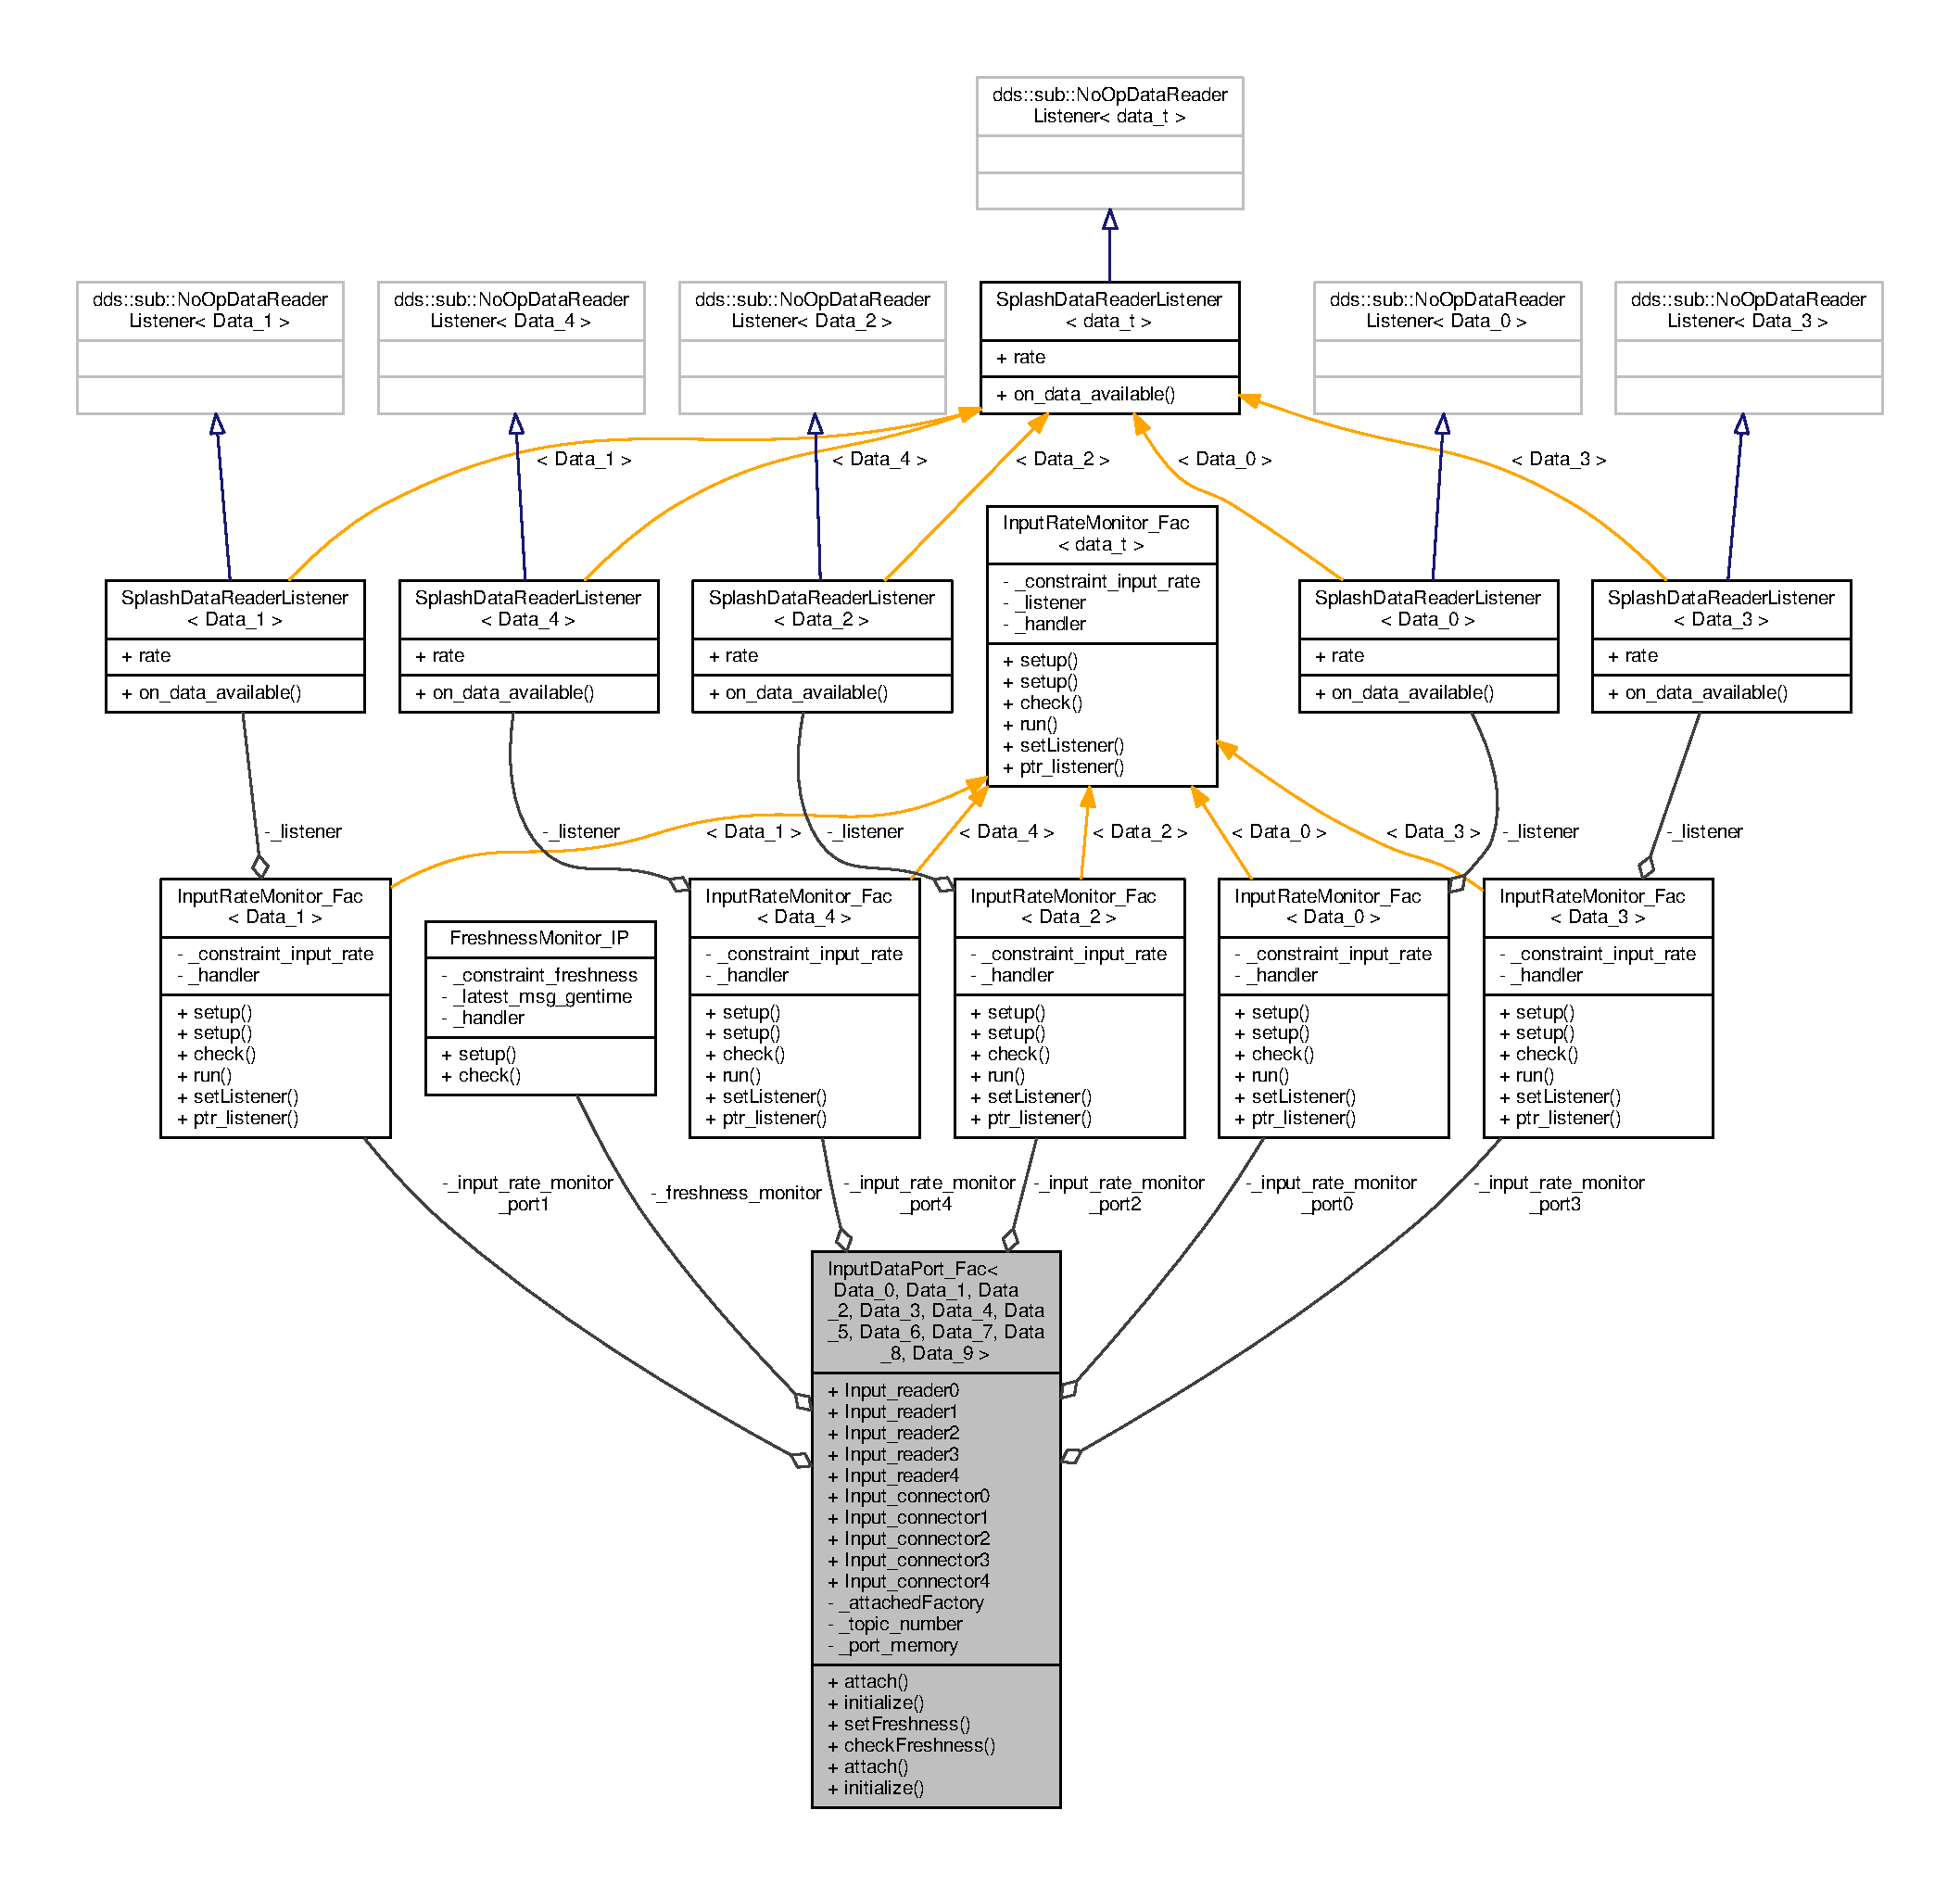
\includegraphics[width=350pt]{classInputDataPort__Fac__coll__graph}
\end{center}
\end{figure}
\subsection*{Public 멤버 함수}
\begin{DoxyCompactItemize}
\item 
int \hyperlink{classInputDataPort__Fac_a510e33d0b638c13d002e8e5bd0732ba5}{attach} (\hyperlink{classFactory}{Factory}$<$ Data\+\_\+0, Data\+\_\+1, Data\+\_\+2, Data\+\_\+3, Data\+\_\+4, Data\+\_\+5, Data\+\_\+6, Data\+\_\+7, Data\+\_\+8, Data\+\_\+9 $>$ $\ast$Fact, std\+::string topic, std\+::string connector\+\_\+topic, int topic\+\_\+number)
\item 
void \hyperlink{classInputDataPort__Fac_adc03c5ac76d6d2565a28fcd36e2c6fc8}{initialize} (int rate, void($\ast$rate\+\_\+handler)(), int freshness, void($\ast$\hyperlink{sample__main_8cpp_ae2b580f894f38496da91bce6c31e186f}{freshness\+\_\+handler})(), bool queueing, int queue\+\_\+size)
\item 
void \hyperlink{classInputDataPort__Fac_a57bb915c4c801305df78d70e3bcb8d5e}{set\+Freshness} (int64\+\_\+t freshness, void($\ast$\hyperlink{sample__main_8cpp_ae2b580f894f38496da91bce6c31e186f}{freshness\+\_\+handler})())
\item 
void \hyperlink{classInputDataPort__Fac_a8074c89d82913aa9be021549578b1212}{check\+Freshness} (int64\+\_\+t msg\+\_\+gentime)
\item 
int \hyperlink{classInputDataPort__Fac_a5d6fc1047ebdd54c3d6cf375b1f6d171}{attach} (\hyperlink{classFactory}{Factory}$<$ Data\+\_\+0, Data\+\_\+1, Data\+\_\+2, Data\+\_\+3, Data\+\_\+4, Data\+\_\+5, Data\+\_\+6, Data\+\_\+7, Data\+\_\+8, Data\+\_\+9 $>$ $\ast$, std\+::string, std\+::string, int)
\item 
void \hyperlink{classInputDataPort__Fac_af5dd3100caaa527c34079201e3297fdc}{initialize} (double, double, bool, int)
\end{DoxyCompactItemize}
\subsection*{Public 속성}
\begin{DoxyCompactItemize}
\item 
dds\+::sub\+::\+Data\+Reader$<$ Data\+\_\+0 $>$ $\ast$ \hyperlink{classInputDataPort__Fac_ad4336e1795b30d34b8fc78209405173c}{Input\+\_\+reader0}
\item 
dds\+::sub\+::\+Data\+Reader$<$ Data\+\_\+1 $>$ $\ast$ \hyperlink{classInputDataPort__Fac_a792017ee994f74bb649bd673ab7fb02a}{Input\+\_\+reader1}
\item 
dds\+::sub\+::\+Data\+Reader$<$ Data\+\_\+2 $>$ $\ast$ \hyperlink{classInputDataPort__Fac_a4a0fff757eea71f4c9d28909442d71ac}{Input\+\_\+reader2}
\item 
dds\+::sub\+::\+Data\+Reader$<$ Data\+\_\+3 $>$ $\ast$ \hyperlink{classInputDataPort__Fac_ac3626a23fa27c43e0a63aa68f022fc2d}{Input\+\_\+reader3}
\item 
dds\+::sub\+::\+Data\+Reader$<$ Data\+\_\+4 $>$ $\ast$ \hyperlink{classInputDataPort__Fac_adfaed3a3a4363088fb1df54b1fb5d6b1}{Input\+\_\+reader4}
\item 
dds\+::pub\+::\+Data\+Writer$<$ Data\+\_\+0 $>$ $\ast$ \hyperlink{classInputDataPort__Fac_af0886b8147a82738272b964c85d0ca28}{Input\+\_\+connector0}
\item 
dds\+::pub\+::\+Data\+Writer$<$ Data\+\_\+1 $>$ $\ast$ \hyperlink{classInputDataPort__Fac_a8f623a6232415353dbbc2243a3c6f148}{Input\+\_\+connector1}
\item 
dds\+::pub\+::\+Data\+Writer$<$ Data\+\_\+2 $>$ $\ast$ \hyperlink{classInputDataPort__Fac_a0f6ab746eaa0b690462afbf40116a4c1}{Input\+\_\+connector2}
\item 
dds\+::pub\+::\+Data\+Writer$<$ Data\+\_\+3 $>$ $\ast$ \hyperlink{classInputDataPort__Fac_a8d08f056c60a03f2218652df61a644e3}{Input\+\_\+connector3}
\item 
dds\+::pub\+::\+Data\+Writer$<$ Data\+\_\+4 $>$ $\ast$ \hyperlink{classInputDataPort__Fac_a67ee8b26e5d0195ddb518e1bc704112b}{Input\+\_\+connector4}
\end{DoxyCompactItemize}
\subsection*{Private 속성}
\begin{DoxyCompactItemize}
\item 
\hyperlink{classFactory}{Factory}$<$ Data\+\_\+0, Data\+\_\+1, Data\+\_\+2, Data\+\_\+3, Data\+\_\+4, Data\+\_\+5, Data\+\_\+6, Data\+\_\+7, Data\+\_\+8, Data\+\_\+9 $>$ $\ast$ \hyperlink{classInputDataPort__Fac_a5978d61d3b32c4610a102e44179ce3c5}{\+\_\+attached\+Factory}
\item 
\hyperlink{classFreshnessMonitor__IP}{Freshness\+Monitor\+\_\+\+IP} \hyperlink{classInputDataPort__Fac_ae9458e7627cc26884a106de9d091d399}{\+\_\+freshness\+\_\+monitor}
\item 
\hyperlink{classInputRateMonitor__Fac}{Input\+Rate\+Monitor\+\_\+\+Fac}$<$ Data\+\_\+0 $>$ \hyperlink{classInputDataPort__Fac_a91153b4dfaf9af79df3223ec7f17eab2}{\+\_\+input\+\_\+rate\+\_\+monitor\+\_\+port0}
\item 
\hyperlink{classInputRateMonitor__Fac}{Input\+Rate\+Monitor\+\_\+\+Fac}$<$ Data\+\_\+1 $>$ \hyperlink{classInputDataPort__Fac_aaff3c7535d1e29e218a6653e7f874e34}{\+\_\+input\+\_\+rate\+\_\+monitor\+\_\+port1}
\item 
\hyperlink{classInputRateMonitor__Fac}{Input\+Rate\+Monitor\+\_\+\+Fac}$<$ Data\+\_\+2 $>$ \hyperlink{classInputDataPort__Fac_afa172d6bd94489f7634ad91440c10a16}{\+\_\+input\+\_\+rate\+\_\+monitor\+\_\+port2}
\item 
\hyperlink{classInputRateMonitor__Fac}{Input\+Rate\+Monitor\+\_\+\+Fac}$<$ Data\+\_\+3 $>$ \hyperlink{classInputDataPort__Fac_a6675cd4e6a4ccb6b2b8c8535aa9cd9f4}{\+\_\+input\+\_\+rate\+\_\+monitor\+\_\+port3}
\item 
\hyperlink{classInputRateMonitor__Fac}{Input\+Rate\+Monitor\+\_\+\+Fac}$<$ Data\+\_\+4 $>$ \hyperlink{classInputDataPort__Fac_a4fe6b7be1eb68bd69bd8fa62e4a3eb2f}{\+\_\+input\+\_\+rate\+\_\+monitor\+\_\+port4}
\item 
int \hyperlink{classInputDataPort__Fac_ad39fee414d67b42e824bad1a16a3bd87}{\+\_\+topic\+\_\+number}
\item 
void $\ast$ \hyperlink{classInputDataPort__Fac_a6c10484e54395bef3479ae6d1bbab04d}{\+\_\+port\+\_\+memory}
\end{DoxyCompactItemize}


\subsection{상세한 설명}
\subsubsection*{template$<$typename Data\+\_\+0, typename Data\+\_\+1, typename Data\+\_\+2, typename Data\+\_\+3, typename Data\+\_\+4, typename Data\+\_\+5, typename Data\+\_\+6, typename Data\+\_\+7, typename Data\+\_\+8, typename Data\+\_\+9$>$\\*
class Input\+Data\+Port\+\_\+\+Fac$<$ Data\+\_\+0, Data\+\_\+1, Data\+\_\+2, Data\+\_\+3, Data\+\_\+4, Data\+\_\+5, Data\+\_\+6, Data\+\_\+7, Data\+\_\+8, Data\+\_\+9 $>$}



Factory.\+cpp 파일의 31 번째 라인에서 정의되었습니다.



\subsection{멤버 함수 문서화}
\index{Input\+Data\+Port\+\_\+\+Fac@{Input\+Data\+Port\+\_\+\+Fac}!attach@{attach}}
\index{attach@{attach}!Input\+Data\+Port\+\_\+\+Fac@{Input\+Data\+Port\+\_\+\+Fac}}
\subsubsection[{\texorpdfstring{attach(\+Factory$<$ Data\+\_\+0, Data\+\_\+1, Data\+\_\+2, Data\+\_\+3, Data\+\_\+4, Data\+\_\+5, Data\+\_\+6, Data\+\_\+7, Data\+\_\+8, Data\+\_\+9 $>$ $\ast$, std\+::string, std\+::string, int)}{attach(Factory< Data_0, Data_1, Data_2, Data_3, Data_4, Data_5, Data_6, Data_7, Data_8, Data_9 > *, std::string, std::string, int)}}]{\setlength{\rightskip}{0pt plus 5cm}template$<$typename Data\+\_\+0 , typename Data\+\_\+1 , typename Data\+\_\+2 , typename Data\+\_\+3 , typename Data\+\_\+4 , typename Data\+\_\+5 , typename Data\+\_\+6 , typename Data\+\_\+7 , typename Data\+\_\+8 , typename Data\+\_\+9 $>$ int {\bf Input\+Data\+Port\+\_\+\+Fac}$<$ Data\+\_\+0, Data\+\_\+1, Data\+\_\+2, Data\+\_\+3, Data\+\_\+4, Data\+\_\+5, Data\+\_\+6, Data\+\_\+7, Data\+\_\+8, Data\+\_\+9 $>$\+::attach (
\begin{DoxyParamCaption}
\item[{{\bf Factory}$<$ Data\+\_\+0, Data\+\_\+1, Data\+\_\+2, Data\+\_\+3, Data\+\_\+4, Data\+\_\+5, Data\+\_\+6, Data\+\_\+7, Data\+\_\+8, Data\+\_\+9 $>$ $\ast$}]{, }
\item[{std\+::string}]{, }
\item[{std\+::string}]{, }
\item[{int}]{}
\end{DoxyParamCaption}
)}\hypertarget{classInputDataPort__Fac_a5d6fc1047ebdd54c3d6cf375b1f6d171}{}\label{classInputDataPort__Fac_a5d6fc1047ebdd54c3d6cf375b1f6d171}
\index{Input\+Data\+Port\+\_\+\+Fac@{Input\+Data\+Port\+\_\+\+Fac}!attach@{attach}}
\index{attach@{attach}!Input\+Data\+Port\+\_\+\+Fac@{Input\+Data\+Port\+\_\+\+Fac}}
\subsubsection[{\texorpdfstring{attach(\+Factory$<$ Data\+\_\+0, Data\+\_\+1, Data\+\_\+2, Data\+\_\+3, Data\+\_\+4, Data\+\_\+5, Data\+\_\+6, Data\+\_\+7, Data\+\_\+8, Data\+\_\+9 $>$ $\ast$\+Fact, std\+::string topic, std\+::string connector\+\_\+topic, int topic\+\_\+number)}{attach(Factory< Data_0, Data_1, Data_2, Data_3, Data_4, Data_5, Data_6, Data_7, Data_8, Data_9 > *Fact, std::string topic, std::string connector_topic, int topic_number)}}]{\setlength{\rightskip}{0pt plus 5cm}template$<$typename Data\+\_\+0 , typename Data\+\_\+1 , typename Data\+\_\+2 , typename Data\+\_\+3 , typename Data\+\_\+4 , typename Data\+\_\+5 , typename Data\+\_\+6 , typename Data\+\_\+7 , typename Data\+\_\+8 , typename Data\+\_\+9 $>$ int {\bf Input\+Data\+Port\+\_\+\+Fac}$<$ Data\+\_\+0, Data\+\_\+1, Data\+\_\+2, Data\+\_\+3, Data\+\_\+4, Data\+\_\+5, Data\+\_\+6, Data\+\_\+7, Data\+\_\+8, Data\+\_\+9 $>$\+::attach (
\begin{DoxyParamCaption}
\item[{{\bf Factory}$<$ Data\+\_\+0, Data\+\_\+1, Data\+\_\+2, Data\+\_\+3, Data\+\_\+4, Data\+\_\+5, Data\+\_\+6, Data\+\_\+7, Data\+\_\+8, Data\+\_\+9 $>$ $\ast$}]{Fact, }
\item[{std\+::string}]{topic, }
\item[{std\+::string}]{connector\+\_\+topic, }
\item[{int}]{topic\+\_\+number}
\end{DoxyParamCaption}
)}\hypertarget{classInputDataPort__Fac_a510e33d0b638c13d002e8e5bd0732ba5}{}\label{classInputDataPort__Fac_a510e33d0b638c13d002e8e5bd0732ba5}


Factory.\+cpp 파일의 473 번째 라인에서 정의되었습니다.



다음을 참조함 \+:  Factory$<$ Data\+\_\+0, Data\+\_\+1, Data\+\_\+2, Data\+\_\+3, Data\+\_\+4, Data\+\_\+5, Data\+\_\+6, Data\+\_\+7, Data\+\_\+8, Data\+\_\+9 $>$\+::connected\+\_\+ports, Factory$<$ Data\+\_\+0, Data\+\_\+1, Data\+\_\+2, Data\+\_\+3, Data\+\_\+4, Data\+\_\+5, Data\+\_\+6, Data\+\_\+7, Data\+\_\+8, Data\+\_\+9 $>$\+::connector\+\_\+topic0, Factory$<$ Data\+\_\+0, Data\+\_\+1, Data\+\_\+2, Data\+\_\+3, Data\+\_\+4, Data\+\_\+5, Data\+\_\+6, Data\+\_\+7, Data\+\_\+8, Data\+\_\+9 $>$\+::connector\+\_\+topic1, Factory$<$ Data\+\_\+0, Data\+\_\+1, Data\+\_\+2, Data\+\_\+3, Data\+\_\+4, Data\+\_\+5, Data\+\_\+6, Data\+\_\+7, Data\+\_\+8, Data\+\_\+9 $>$\+::connector\+\_\+topic2, Factory$<$ Data\+\_\+0, Data\+\_\+1, Data\+\_\+2, Data\+\_\+3, Data\+\_\+4, Data\+\_\+5, Data\+\_\+6, Data\+\_\+7, Data\+\_\+8, Data\+\_\+9 $>$\+::connector\+\_\+topic3, Factory$<$ Data\+\_\+0, Data\+\_\+1, Data\+\_\+2, Data\+\_\+3, Data\+\_\+4, Data\+\_\+5, Data\+\_\+6, Data\+\_\+7, Data\+\_\+8, Data\+\_\+9 $>$\+::connector\+\_\+topic4, Factory$<$ Data\+\_\+0, Data\+\_\+1, Data\+\_\+2, Data\+\_\+3, Data\+\_\+4, Data\+\_\+5, Data\+\_\+6, Data\+\_\+7, Data\+\_\+8, Data\+\_\+9 $>$\+::\+I\+D\+P0, Factory$<$ Data\+\_\+0, Data\+\_\+1, Data\+\_\+2, Data\+\_\+3, Data\+\_\+4, Data\+\_\+5, Data\+\_\+6, Data\+\_\+7, Data\+\_\+8, Data\+\_\+9 $>$\+::\+I\+D\+P1, Factory$<$ Data\+\_\+0, Data\+\_\+1, Data\+\_\+2, Data\+\_\+3, Data\+\_\+4, Data\+\_\+5, Data\+\_\+6, Data\+\_\+7, Data\+\_\+8, Data\+\_\+9 $>$\+::\+I\+D\+P2, Factory$<$ Data\+\_\+0, Data\+\_\+1, Data\+\_\+2, Data\+\_\+3, Data\+\_\+4, Data\+\_\+5, Data\+\_\+6, Data\+\_\+7, Data\+\_\+8, Data\+\_\+9 $>$\+::\+I\+D\+P3, Factory$<$ Data\+\_\+0, Data\+\_\+1, Data\+\_\+2, Data\+\_\+3, Data\+\_\+4, Data\+\_\+5, Data\+\_\+6, Data\+\_\+7, Data\+\_\+8, Data\+\_\+9 $>$\+::\+I\+D\+P4, Input\+Rate\+Monitor\+\_\+\+Fac$<$ data\+\_\+t $>$\+::ptr\+\_\+listener(), Input\+Rate\+Monitor\+\_\+\+Fac$<$ data\+\_\+t $>$\+::set\+Listener(), Factory$<$ Data\+\_\+0, Data\+\_\+1, Data\+\_\+2, Data\+\_\+3, Data\+\_\+4, Data\+\_\+5, Data\+\_\+6, Data\+\_\+7, Data\+\_\+8, Data\+\_\+9 $>$\+::topic0, Factory$<$ Data\+\_\+0, Data\+\_\+1, Data\+\_\+2, Data\+\_\+3, Data\+\_\+4, Data\+\_\+5, Data\+\_\+6, Data\+\_\+7, Data\+\_\+8, Data\+\_\+9 $>$\+::topic1, Factory$<$ Data\+\_\+0, Data\+\_\+1, Data\+\_\+2, Data\+\_\+3, Data\+\_\+4, Data\+\_\+5, Data\+\_\+6, Data\+\_\+7, Data\+\_\+8, Data\+\_\+9 $>$\+::topic2, Factory$<$ Data\+\_\+0, Data\+\_\+1, Data\+\_\+2, Data\+\_\+3, Data\+\_\+4, Data\+\_\+5, Data\+\_\+6, Data\+\_\+7, Data\+\_\+8, Data\+\_\+9 $>$\+::topic3, Factory$<$ Data\+\_\+0, Data\+\_\+1, Data\+\_\+2, Data\+\_\+3, Data\+\_\+4, Data\+\_\+5, Data\+\_\+6, Data\+\_\+7, Data\+\_\+8, Data\+\_\+9 $>$\+::topic4.



이 함수 내부에서 호출하는 함수들에 대한 그래프입니다.\+:\nopagebreak
\begin{figure}[H]
\begin{center}
\leavevmode
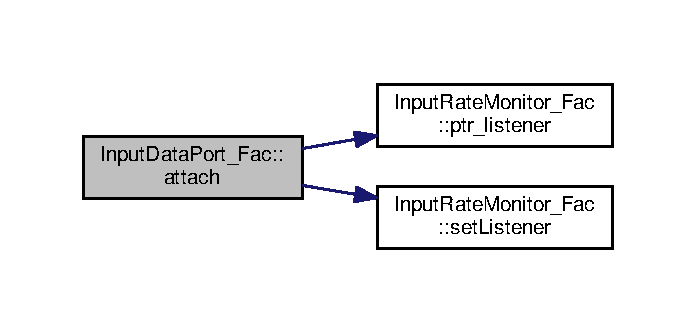
\includegraphics[width=334pt]{classInputDataPort__Fac_a510e33d0b638c13d002e8e5bd0732ba5_cgraph}
\end{center}
\end{figure}


\index{Input\+Data\+Port\+\_\+\+Fac@{Input\+Data\+Port\+\_\+\+Fac}!check\+Freshness@{check\+Freshness}}
\index{check\+Freshness@{check\+Freshness}!Input\+Data\+Port\+\_\+\+Fac@{Input\+Data\+Port\+\_\+\+Fac}}
\subsubsection[{\texorpdfstring{check\+Freshness(int64\+\_\+t msg\+\_\+gentime)}{checkFreshness(int64_t msg_gentime)}}]{\setlength{\rightskip}{0pt plus 5cm}template$<$typename Data\+\_\+0 , typename Data\+\_\+1 , typename Data\+\_\+2 , typename Data\+\_\+3 , typename Data\+\_\+4 , typename Data\+\_\+5 , typename Data\+\_\+6 , typename Data\+\_\+7 , typename Data\+\_\+8 , typename Data\+\_\+9 $>$ void {\bf Input\+Data\+Port\+\_\+\+Fac}$<$ Data\+\_\+0, Data\+\_\+1, Data\+\_\+2, Data\+\_\+3, Data\+\_\+4, Data\+\_\+5, Data\+\_\+6, Data\+\_\+7, Data\+\_\+8, Data\+\_\+9 $>$\+::check\+Freshness (
\begin{DoxyParamCaption}
\item[{int64\+\_\+t}]{msg\+\_\+gentime}
\end{DoxyParamCaption}
)}\hypertarget{classInputDataPort__Fac_a8074c89d82913aa9be021549578b1212}{}\label{classInputDataPort__Fac_a8074c89d82913aa9be021549578b1212}


Factory.\+cpp 파일의 460 번째 라인에서 정의되었습니다.



다음을 참조함 \+:  Freshness\+Monitor\+\_\+\+I\+P\+::check().



이 함수 내부에서 호출하는 함수들에 대한 그래프입니다.\+:\nopagebreak
\begin{figure}[H]
\begin{center}
\leavevmode
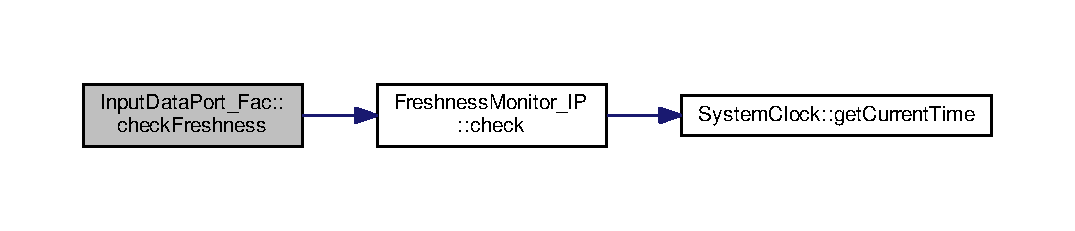
\includegraphics[width=350pt]{classInputDataPort__Fac_a8074c89d82913aa9be021549578b1212_cgraph}
\end{center}
\end{figure}


\index{Input\+Data\+Port\+\_\+\+Fac@{Input\+Data\+Port\+\_\+\+Fac}!initialize@{initialize}}
\index{initialize@{initialize}!Input\+Data\+Port\+\_\+\+Fac@{Input\+Data\+Port\+\_\+\+Fac}}
\subsubsection[{\texorpdfstring{initialize(double, double, bool, int)}{initialize(double, double, bool, int)}}]{\setlength{\rightskip}{0pt plus 5cm}template$<$typename Data\+\_\+0 , typename Data\+\_\+1 , typename Data\+\_\+2 , typename Data\+\_\+3 , typename Data\+\_\+4 , typename Data\+\_\+5 , typename Data\+\_\+6 , typename Data\+\_\+7 , typename Data\+\_\+8 , typename Data\+\_\+9 $>$ void {\bf Input\+Data\+Port\+\_\+\+Fac}$<$ Data\+\_\+0, Data\+\_\+1, Data\+\_\+2, Data\+\_\+3, Data\+\_\+4, Data\+\_\+5, Data\+\_\+6, Data\+\_\+7, Data\+\_\+8, Data\+\_\+9 $>$\+::initialize (
\begin{DoxyParamCaption}
\item[{double}]{rate, }
\item[{double}]{freshness, }
\item[{bool}]{queueing, }
\item[{int}]{queue\+\_\+size}
\end{DoxyParamCaption}
)}\hypertarget{classInputDataPort__Fac_af5dd3100caaa527c34079201e3297fdc}{}\label{classInputDataPort__Fac_af5dd3100caaa527c34079201e3297fdc}


Factory\+\_\+old.\+cpp 파일의 319 번째 라인에서 정의되었습니다.



다음을 참조함 \+:  Output\+Data\+Port\+\_\+\+Fac$<$ Data\+\_\+0, Data\+\_\+1, Data\+\_\+2, Data\+\_\+3, Data\+\_\+4, Data\+\_\+5, Data\+\_\+6, Data\+\_\+7, Data\+\_\+8, Data\+\_\+9 $>$\+::attach(), Factory$<$ Data\+\_\+0, Data\+\_\+1, Data\+\_\+2, Data\+\_\+3, Data\+\_\+4, Data\+\_\+5, Data\+\_\+6, Data\+\_\+7, Data\+\_\+8, Data\+\_\+9 $>$\+::connected\+\_\+ports, Factory$<$ Data\+\_\+0, Data\+\_\+1, Data\+\_\+2, Data\+\_\+3, Data\+\_\+4, Data\+\_\+5, Data\+\_\+6, Data\+\_\+7, Data\+\_\+8, Data\+\_\+9 $>$\+::connector\+\_\+topic5, Factory$<$ Data\+\_\+0, Data\+\_\+1, Data\+\_\+2, Data\+\_\+3, Data\+\_\+4, Data\+\_\+5, Data\+\_\+6, Data\+\_\+7, Data\+\_\+8, Data\+\_\+9 $>$\+::connector\+\_\+topic6, Factory$<$ Data\+\_\+0, Data\+\_\+1, Data\+\_\+2, Data\+\_\+3, Data\+\_\+4, Data\+\_\+5, Data\+\_\+6, Data\+\_\+7, Data\+\_\+8, Data\+\_\+9 $>$\+::connector\+\_\+topic7, Factory$<$ Data\+\_\+0, Data\+\_\+1, Data\+\_\+2, Data\+\_\+3, Data\+\_\+4, Data\+\_\+5, Data\+\_\+6, Data\+\_\+7, Data\+\_\+8, Data\+\_\+9 $>$\+::connector\+\_\+topic8, Factory$<$ Data\+\_\+0, Data\+\_\+1, Data\+\_\+2, Data\+\_\+3, Data\+\_\+4, Data\+\_\+5, Data\+\_\+6, Data\+\_\+7, Data\+\_\+8, Data\+\_\+9 $>$\+::connector\+\_\+topic9, Factory$<$ Data\+\_\+0, Data\+\_\+1, Data\+\_\+2, Data\+\_\+3, Data\+\_\+4, Data\+\_\+5, Data\+\_\+6, Data\+\_\+7, Data\+\_\+8, Data\+\_\+9 $>$\+::initialize(), Factory$<$ Data\+\_\+0, Data\+\_\+1, Data\+\_\+2, Data\+\_\+3, Data\+\_\+4, Data\+\_\+5, Data\+\_\+6, Data\+\_\+7, Data\+\_\+8, Data\+\_\+9 $>$\+::\+O\+D\+P0, Factory$<$ Data\+\_\+0, Data\+\_\+1, Data\+\_\+2, Data\+\_\+3, Data\+\_\+4, Data\+\_\+5, Data\+\_\+6, Data\+\_\+7, Data\+\_\+8, Data\+\_\+9 $>$\+::\+O\+D\+P1, Factory$<$ Data\+\_\+0, Data\+\_\+1, Data\+\_\+2, Data\+\_\+3, Data\+\_\+4, Data\+\_\+5, Data\+\_\+6, Data\+\_\+7, Data\+\_\+8, Data\+\_\+9 $>$\+::\+O\+D\+P2, Factory$<$ Data\+\_\+0, Data\+\_\+1, Data\+\_\+2, Data\+\_\+3, Data\+\_\+4, Data\+\_\+5, Data\+\_\+6, Data\+\_\+7, Data\+\_\+8, Data\+\_\+9 $>$\+::\+O\+D\+P3, Factory$<$ Data\+\_\+0, Data\+\_\+1, Data\+\_\+2, Data\+\_\+3, Data\+\_\+4, Data\+\_\+5, Data\+\_\+6, Data\+\_\+7, Data\+\_\+8, Data\+\_\+9 $>$\+::\+O\+D\+P4, Factory$<$ Data\+\_\+0, Data\+\_\+1, Data\+\_\+2, Data\+\_\+3, Data\+\_\+4, Data\+\_\+5, Data\+\_\+6, Data\+\_\+7, Data\+\_\+8, Data\+\_\+9 $>$\+::topic5, Factory$<$ Data\+\_\+0, Data\+\_\+1, Data\+\_\+2, Data\+\_\+3, Data\+\_\+4, Data\+\_\+5, Data\+\_\+6, Data\+\_\+7, Data\+\_\+8, Data\+\_\+9 $>$\+::topic6, Factory$<$ Data\+\_\+0, Data\+\_\+1, Data\+\_\+2, Data\+\_\+3, Data\+\_\+4, Data\+\_\+5, Data\+\_\+6, Data\+\_\+7, Data\+\_\+8, Data\+\_\+9 $>$\+::topic7, Factory$<$ Data\+\_\+0, Data\+\_\+1, Data\+\_\+2, Data\+\_\+3, Data\+\_\+4, Data\+\_\+5, Data\+\_\+6, Data\+\_\+7, Data\+\_\+8, Data\+\_\+9 $>$\+::topic8, Factory$<$ Data\+\_\+0, Data\+\_\+1, Data\+\_\+2, Data\+\_\+3, Data\+\_\+4, Data\+\_\+5, Data\+\_\+6, Data\+\_\+7, Data\+\_\+8, Data\+\_\+9 $>$\+::topic9.



이 함수 내부에서 호출하는 함수들에 대한 그래프입니다.\+:\nopagebreak
\begin{figure}[H]
\begin{center}
\leavevmode
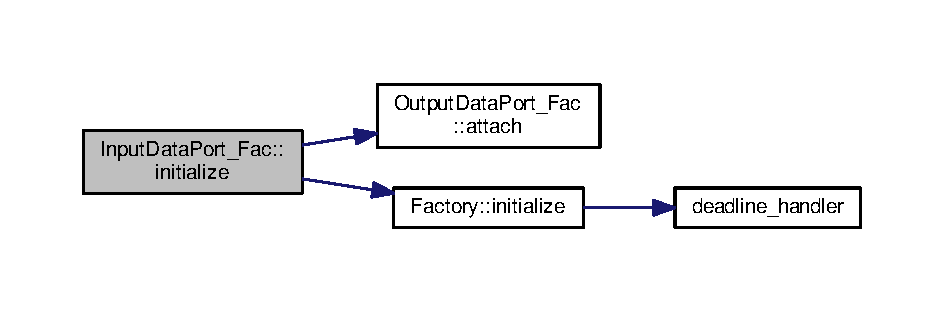
\includegraphics[width=350pt]{classInputDataPort__Fac_af5dd3100caaa527c34079201e3297fdc_cgraph}
\end{center}
\end{figure}


\index{Input\+Data\+Port\+\_\+\+Fac@{Input\+Data\+Port\+\_\+\+Fac}!initialize@{initialize}}
\index{initialize@{initialize}!Input\+Data\+Port\+\_\+\+Fac@{Input\+Data\+Port\+\_\+\+Fac}}
\subsubsection[{\texorpdfstring{initialize(int rate, void($\ast$rate\+\_\+handler)(), int freshness, void($\ast$freshness\+\_\+handler)(), bool queueing, int queue\+\_\+size)}{initialize(int rate, void(*rate_handler)(), int freshness, void(*freshness_handler)(), bool queueing, int queue_size)}}]{\setlength{\rightskip}{0pt plus 5cm}template$<$typename Data\+\_\+0 , typename Data\+\_\+1 , typename Data\+\_\+2 , typename Data\+\_\+3 , typename Data\+\_\+4 , typename Data\+\_\+5 , typename Data\+\_\+6 , typename Data\+\_\+7 , typename Data\+\_\+8 , typename Data\+\_\+9 $>$ void {\bf Input\+Data\+Port\+\_\+\+Fac}$<$ Data\+\_\+0, Data\+\_\+1, Data\+\_\+2, Data\+\_\+3, Data\+\_\+4, Data\+\_\+5, Data\+\_\+6, Data\+\_\+7, Data\+\_\+8, Data\+\_\+9 $>$\+::initialize (
\begin{DoxyParamCaption}
\item[{int}]{rate, }
\item[{void($\ast$)()}]{rate\+\_\+handler, }
\item[{int}]{freshness, }
\item[{void($\ast$)()}]{freshness\+\_\+handler, }
\item[{bool}]{queueing, }
\item[{int}]{queue\+\_\+size}
\end{DoxyParamCaption}
)}\hypertarget{classInputDataPort__Fac_adc03c5ac76d6d2565a28fcd36e2c6fc8}{}\label{classInputDataPort__Fac_adc03c5ac76d6d2565a28fcd36e2c6fc8}


Factory.\+cpp 파일의 588 번째 라인에서 정의되었습니다.



다음을 참조함 \+:  freshness\+\_\+handler(), Input\+Rate\+Monitor\+\_\+\+Fac$<$ data\+\_\+t $>$\+::run(), Input\+Rate\+Monitor\+\_\+\+Fac$<$ data\+\_\+t $>$\+::setup().



이 함수 내부에서 호출하는 함수들에 대한 그래프입니다.\+:\nopagebreak
\begin{figure}[H]
\begin{center}
\leavevmode
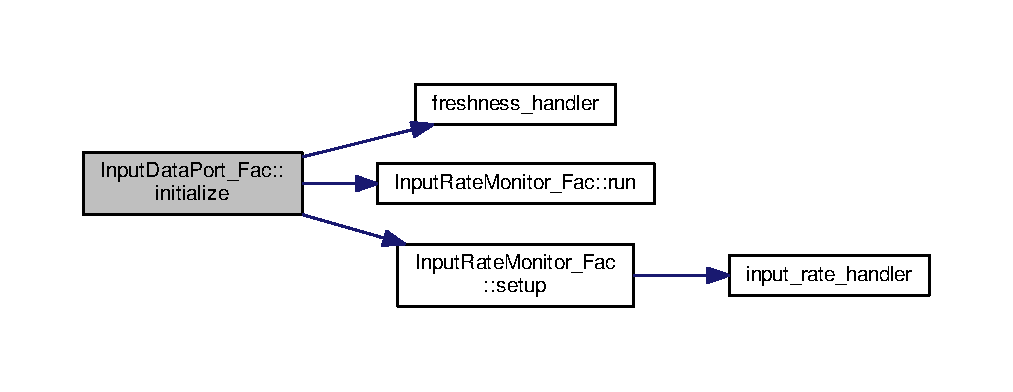
\includegraphics[width=350pt]{classInputDataPort__Fac_adc03c5ac76d6d2565a28fcd36e2c6fc8_cgraph}
\end{center}
\end{figure}


\index{Input\+Data\+Port\+\_\+\+Fac@{Input\+Data\+Port\+\_\+\+Fac}!set\+Freshness@{set\+Freshness}}
\index{set\+Freshness@{set\+Freshness}!Input\+Data\+Port\+\_\+\+Fac@{Input\+Data\+Port\+\_\+\+Fac}}
\subsubsection[{\texorpdfstring{set\+Freshness(int64\+\_\+t freshness, void($\ast$freshness\+\_\+handler)())}{setFreshness(int64_t freshness, void(*freshness_handler)())}}]{\setlength{\rightskip}{0pt plus 5cm}template$<$typename Data\+\_\+0 , typename Data\+\_\+1 , typename Data\+\_\+2 , typename Data\+\_\+3 , typename Data\+\_\+4 , typename Data\+\_\+5 , typename Data\+\_\+6 , typename Data\+\_\+7 , typename Data\+\_\+8 , typename Data\+\_\+9 $>$ void {\bf Input\+Data\+Port\+\_\+\+Fac}$<$ Data\+\_\+0, Data\+\_\+1, Data\+\_\+2, Data\+\_\+3, Data\+\_\+4, Data\+\_\+5, Data\+\_\+6, Data\+\_\+7, Data\+\_\+8, Data\+\_\+9 $>$\+::set\+Freshness (
\begin{DoxyParamCaption}
\item[{int64\+\_\+t}]{freshness, }
\item[{void($\ast$)()}]{freshness\+\_\+handler}
\end{DoxyParamCaption}
)}\hypertarget{classInputDataPort__Fac_a57bb915c4c801305df78d70e3bcb8d5e}{}\label{classInputDataPort__Fac_a57bb915c4c801305df78d70e3bcb8d5e}


Factory.\+cpp 파일의 448 번째 라인에서 정의되었습니다.



다음을 참조함 \+:  freshness\+\_\+handler(), Freshness\+Monitor\+\_\+\+I\+P\+::setup().



이 함수 내부에서 호출하는 함수들에 대한 그래프입니다.\+:\nopagebreak
\begin{figure}[H]
\begin{center}
\leavevmode
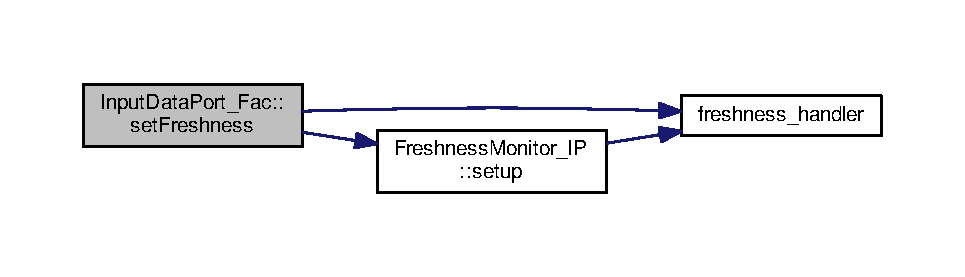
\includegraphics[width=350pt]{classInputDataPort__Fac_a57bb915c4c801305df78d70e3bcb8d5e_cgraph}
\end{center}
\end{figure}




\subsection{멤버 데이타 문서화}
\index{Input\+Data\+Port\+\_\+\+Fac@{Input\+Data\+Port\+\_\+\+Fac}!\+\_\+attached\+Factory@{\+\_\+attached\+Factory}}
\index{\+\_\+attached\+Factory@{\+\_\+attached\+Factory}!Input\+Data\+Port\+\_\+\+Fac@{Input\+Data\+Port\+\_\+\+Fac}}
\subsubsection[{\texorpdfstring{\+\_\+attached\+Factory}{_attachedFactory}}]{\setlength{\rightskip}{0pt plus 5cm}template$<$typename Data\+\_\+0 , typename Data\+\_\+1 , typename Data\+\_\+2 , typename Data\+\_\+3 , typename Data\+\_\+4 , typename Data\+\_\+5 , typename Data\+\_\+6 , typename Data\+\_\+7 , typename Data\+\_\+8 , typename Data\+\_\+9 $>$ {\bf Factory}$<$Data\+\_\+0,Data\+\_\+1,Data\+\_\+2,Data\+\_\+3,Data\+\_\+4,Data\+\_\+5,Data\+\_\+6,Data\+\_\+7,Data\+\_\+8,Data\+\_\+9$>$$\ast$ {\bf Input\+Data\+Port\+\_\+\+Fac}$<$ Data\+\_\+0, Data\+\_\+1, Data\+\_\+2, Data\+\_\+3, Data\+\_\+4, Data\+\_\+5, Data\+\_\+6, Data\+\_\+7, Data\+\_\+8, Data\+\_\+9 $>$\+::\+\_\+attached\+Factory\hspace{0.3cm}{\ttfamily [private]}}\hypertarget{classInputDataPort__Fac_a5978d61d3b32c4610a102e44179ce3c5}{}\label{classInputDataPort__Fac_a5978d61d3b32c4610a102e44179ce3c5}


Factory.\+cpp 파일의 406 번째 라인에서 정의되었습니다.

\index{Input\+Data\+Port\+\_\+\+Fac@{Input\+Data\+Port\+\_\+\+Fac}!\+\_\+freshness\+\_\+monitor@{\+\_\+freshness\+\_\+monitor}}
\index{\+\_\+freshness\+\_\+monitor@{\+\_\+freshness\+\_\+monitor}!Input\+Data\+Port\+\_\+\+Fac@{Input\+Data\+Port\+\_\+\+Fac}}
\subsubsection[{\texorpdfstring{\+\_\+freshness\+\_\+monitor}{_freshness_monitor}}]{\setlength{\rightskip}{0pt plus 5cm}template$<$typename Data\+\_\+0 , typename Data\+\_\+1 , typename Data\+\_\+2 , typename Data\+\_\+3 , typename Data\+\_\+4 , typename Data\+\_\+5 , typename Data\+\_\+6 , typename Data\+\_\+7 , typename Data\+\_\+8 , typename Data\+\_\+9 $>$ {\bf Freshness\+Monitor\+\_\+\+IP} {\bf Input\+Data\+Port\+\_\+\+Fac}$<$ Data\+\_\+0, Data\+\_\+1, Data\+\_\+2, Data\+\_\+3, Data\+\_\+4, Data\+\_\+5, Data\+\_\+6, Data\+\_\+7, Data\+\_\+8, Data\+\_\+9 $>$\+::\+\_\+freshness\+\_\+monitor\hspace{0.3cm}{\ttfamily [private]}}\hypertarget{classInputDataPort__Fac_ae9458e7627cc26884a106de9d091d399}{}\label{classInputDataPort__Fac_ae9458e7627cc26884a106de9d091d399}


Factory.\+cpp 파일의 408 번째 라인에서 정의되었습니다.

\index{Input\+Data\+Port\+\_\+\+Fac@{Input\+Data\+Port\+\_\+\+Fac}!\+\_\+input\+\_\+rate\+\_\+monitor\+\_\+port0@{\+\_\+input\+\_\+rate\+\_\+monitor\+\_\+port0}}
\index{\+\_\+input\+\_\+rate\+\_\+monitor\+\_\+port0@{\+\_\+input\+\_\+rate\+\_\+monitor\+\_\+port0}!Input\+Data\+Port\+\_\+\+Fac@{Input\+Data\+Port\+\_\+\+Fac}}
\subsubsection[{\texorpdfstring{\+\_\+input\+\_\+rate\+\_\+monitor\+\_\+port0}{_input_rate_monitor_port0}}]{\setlength{\rightskip}{0pt plus 5cm}template$<$typename Data\+\_\+0 , typename Data\+\_\+1 , typename Data\+\_\+2 , typename Data\+\_\+3 , typename Data\+\_\+4 , typename Data\+\_\+5 , typename Data\+\_\+6 , typename Data\+\_\+7 , typename Data\+\_\+8 , typename Data\+\_\+9 $>$ {\bf Input\+Rate\+Monitor\+\_\+\+Fac}$<$Data\+\_\+0$>$ {\bf Input\+Data\+Port\+\_\+\+Fac}$<$ Data\+\_\+0, Data\+\_\+1, Data\+\_\+2, Data\+\_\+3, Data\+\_\+4, Data\+\_\+5, Data\+\_\+6, Data\+\_\+7, Data\+\_\+8, Data\+\_\+9 $>$\+::\+\_\+input\+\_\+rate\+\_\+monitor\+\_\+port0\hspace{0.3cm}{\ttfamily [private]}}\hypertarget{classInputDataPort__Fac_a91153b4dfaf9af79df3223ec7f17eab2}{}\label{classInputDataPort__Fac_a91153b4dfaf9af79df3223ec7f17eab2}


Factory.\+cpp 파일의 410 번째 라인에서 정의되었습니다.

\index{Input\+Data\+Port\+\_\+\+Fac@{Input\+Data\+Port\+\_\+\+Fac}!\+\_\+input\+\_\+rate\+\_\+monitor\+\_\+port1@{\+\_\+input\+\_\+rate\+\_\+monitor\+\_\+port1}}
\index{\+\_\+input\+\_\+rate\+\_\+monitor\+\_\+port1@{\+\_\+input\+\_\+rate\+\_\+monitor\+\_\+port1}!Input\+Data\+Port\+\_\+\+Fac@{Input\+Data\+Port\+\_\+\+Fac}}
\subsubsection[{\texorpdfstring{\+\_\+input\+\_\+rate\+\_\+monitor\+\_\+port1}{_input_rate_monitor_port1}}]{\setlength{\rightskip}{0pt plus 5cm}template$<$typename Data\+\_\+0 , typename Data\+\_\+1 , typename Data\+\_\+2 , typename Data\+\_\+3 , typename Data\+\_\+4 , typename Data\+\_\+5 , typename Data\+\_\+6 , typename Data\+\_\+7 , typename Data\+\_\+8 , typename Data\+\_\+9 $>$ {\bf Input\+Rate\+Monitor\+\_\+\+Fac}$<$Data\+\_\+1$>$ {\bf Input\+Data\+Port\+\_\+\+Fac}$<$ Data\+\_\+0, Data\+\_\+1, Data\+\_\+2, Data\+\_\+3, Data\+\_\+4, Data\+\_\+5, Data\+\_\+6, Data\+\_\+7, Data\+\_\+8, Data\+\_\+9 $>$\+::\+\_\+input\+\_\+rate\+\_\+monitor\+\_\+port1\hspace{0.3cm}{\ttfamily [private]}}\hypertarget{classInputDataPort__Fac_aaff3c7535d1e29e218a6653e7f874e34}{}\label{classInputDataPort__Fac_aaff3c7535d1e29e218a6653e7f874e34}


Factory.\+cpp 파일의 411 번째 라인에서 정의되었습니다.

\index{Input\+Data\+Port\+\_\+\+Fac@{Input\+Data\+Port\+\_\+\+Fac}!\+\_\+input\+\_\+rate\+\_\+monitor\+\_\+port2@{\+\_\+input\+\_\+rate\+\_\+monitor\+\_\+port2}}
\index{\+\_\+input\+\_\+rate\+\_\+monitor\+\_\+port2@{\+\_\+input\+\_\+rate\+\_\+monitor\+\_\+port2}!Input\+Data\+Port\+\_\+\+Fac@{Input\+Data\+Port\+\_\+\+Fac}}
\subsubsection[{\texorpdfstring{\+\_\+input\+\_\+rate\+\_\+monitor\+\_\+port2}{_input_rate_monitor_port2}}]{\setlength{\rightskip}{0pt plus 5cm}template$<$typename Data\+\_\+0 , typename Data\+\_\+1 , typename Data\+\_\+2 , typename Data\+\_\+3 , typename Data\+\_\+4 , typename Data\+\_\+5 , typename Data\+\_\+6 , typename Data\+\_\+7 , typename Data\+\_\+8 , typename Data\+\_\+9 $>$ {\bf Input\+Rate\+Monitor\+\_\+\+Fac}$<$Data\+\_\+2$>$ {\bf Input\+Data\+Port\+\_\+\+Fac}$<$ Data\+\_\+0, Data\+\_\+1, Data\+\_\+2, Data\+\_\+3, Data\+\_\+4, Data\+\_\+5, Data\+\_\+6, Data\+\_\+7, Data\+\_\+8, Data\+\_\+9 $>$\+::\+\_\+input\+\_\+rate\+\_\+monitor\+\_\+port2\hspace{0.3cm}{\ttfamily [private]}}\hypertarget{classInputDataPort__Fac_afa172d6bd94489f7634ad91440c10a16}{}\label{classInputDataPort__Fac_afa172d6bd94489f7634ad91440c10a16}


Factory.\+cpp 파일의 412 번째 라인에서 정의되었습니다.

\index{Input\+Data\+Port\+\_\+\+Fac@{Input\+Data\+Port\+\_\+\+Fac}!\+\_\+input\+\_\+rate\+\_\+monitor\+\_\+port3@{\+\_\+input\+\_\+rate\+\_\+monitor\+\_\+port3}}
\index{\+\_\+input\+\_\+rate\+\_\+monitor\+\_\+port3@{\+\_\+input\+\_\+rate\+\_\+monitor\+\_\+port3}!Input\+Data\+Port\+\_\+\+Fac@{Input\+Data\+Port\+\_\+\+Fac}}
\subsubsection[{\texorpdfstring{\+\_\+input\+\_\+rate\+\_\+monitor\+\_\+port3}{_input_rate_monitor_port3}}]{\setlength{\rightskip}{0pt plus 5cm}template$<$typename Data\+\_\+0 , typename Data\+\_\+1 , typename Data\+\_\+2 , typename Data\+\_\+3 , typename Data\+\_\+4 , typename Data\+\_\+5 , typename Data\+\_\+6 , typename Data\+\_\+7 , typename Data\+\_\+8 , typename Data\+\_\+9 $>$ {\bf Input\+Rate\+Monitor\+\_\+\+Fac}$<$Data\+\_\+3$>$ {\bf Input\+Data\+Port\+\_\+\+Fac}$<$ Data\+\_\+0, Data\+\_\+1, Data\+\_\+2, Data\+\_\+3, Data\+\_\+4, Data\+\_\+5, Data\+\_\+6, Data\+\_\+7, Data\+\_\+8, Data\+\_\+9 $>$\+::\+\_\+input\+\_\+rate\+\_\+monitor\+\_\+port3\hspace{0.3cm}{\ttfamily [private]}}\hypertarget{classInputDataPort__Fac_a6675cd4e6a4ccb6b2b8c8535aa9cd9f4}{}\label{classInputDataPort__Fac_a6675cd4e6a4ccb6b2b8c8535aa9cd9f4}


Factory.\+cpp 파일의 413 번째 라인에서 정의되었습니다.

\index{Input\+Data\+Port\+\_\+\+Fac@{Input\+Data\+Port\+\_\+\+Fac}!\+\_\+input\+\_\+rate\+\_\+monitor\+\_\+port4@{\+\_\+input\+\_\+rate\+\_\+monitor\+\_\+port4}}
\index{\+\_\+input\+\_\+rate\+\_\+monitor\+\_\+port4@{\+\_\+input\+\_\+rate\+\_\+monitor\+\_\+port4}!Input\+Data\+Port\+\_\+\+Fac@{Input\+Data\+Port\+\_\+\+Fac}}
\subsubsection[{\texorpdfstring{\+\_\+input\+\_\+rate\+\_\+monitor\+\_\+port4}{_input_rate_monitor_port4}}]{\setlength{\rightskip}{0pt plus 5cm}template$<$typename Data\+\_\+0 , typename Data\+\_\+1 , typename Data\+\_\+2 , typename Data\+\_\+3 , typename Data\+\_\+4 , typename Data\+\_\+5 , typename Data\+\_\+6 , typename Data\+\_\+7 , typename Data\+\_\+8 , typename Data\+\_\+9 $>$ {\bf Input\+Rate\+Monitor\+\_\+\+Fac}$<$Data\+\_\+4$>$ {\bf Input\+Data\+Port\+\_\+\+Fac}$<$ Data\+\_\+0, Data\+\_\+1, Data\+\_\+2, Data\+\_\+3, Data\+\_\+4, Data\+\_\+5, Data\+\_\+6, Data\+\_\+7, Data\+\_\+8, Data\+\_\+9 $>$\+::\+\_\+input\+\_\+rate\+\_\+monitor\+\_\+port4\hspace{0.3cm}{\ttfamily [private]}}\hypertarget{classInputDataPort__Fac_a4fe6b7be1eb68bd69bd8fa62e4a3eb2f}{}\label{classInputDataPort__Fac_a4fe6b7be1eb68bd69bd8fa62e4a3eb2f}


Factory.\+cpp 파일의 414 번째 라인에서 정의되었습니다.

\index{Input\+Data\+Port\+\_\+\+Fac@{Input\+Data\+Port\+\_\+\+Fac}!\+\_\+port\+\_\+memory@{\+\_\+port\+\_\+memory}}
\index{\+\_\+port\+\_\+memory@{\+\_\+port\+\_\+memory}!Input\+Data\+Port\+\_\+\+Fac@{Input\+Data\+Port\+\_\+\+Fac}}
\subsubsection[{\texorpdfstring{\+\_\+port\+\_\+memory}{_port_memory}}]{\setlength{\rightskip}{0pt plus 5cm}template$<$typename Data\+\_\+0 , typename Data\+\_\+1 , typename Data\+\_\+2 , typename Data\+\_\+3 , typename Data\+\_\+4 , typename Data\+\_\+5 , typename Data\+\_\+6 , typename Data\+\_\+7 , typename Data\+\_\+8 , typename Data\+\_\+9 $>$ void$\ast$ {\bf Input\+Data\+Port\+\_\+\+Fac}$<$ Data\+\_\+0, Data\+\_\+1, Data\+\_\+2, Data\+\_\+3, Data\+\_\+4, Data\+\_\+5, Data\+\_\+6, Data\+\_\+7, Data\+\_\+8, Data\+\_\+9 $>$\+::\+\_\+port\+\_\+memory\hspace{0.3cm}{\ttfamily [private]}}\hypertarget{classInputDataPort__Fac_a6c10484e54395bef3479ae6d1bbab04d}{}\label{classInputDataPort__Fac_a6c10484e54395bef3479ae6d1bbab04d}


Factory.\+cpp 파일의 417 번째 라인에서 정의되었습니다.

\index{Input\+Data\+Port\+\_\+\+Fac@{Input\+Data\+Port\+\_\+\+Fac}!\+\_\+topic\+\_\+number@{\+\_\+topic\+\_\+number}}
\index{\+\_\+topic\+\_\+number@{\+\_\+topic\+\_\+number}!Input\+Data\+Port\+\_\+\+Fac@{Input\+Data\+Port\+\_\+\+Fac}}
\subsubsection[{\texorpdfstring{\+\_\+topic\+\_\+number}{_topic_number}}]{\setlength{\rightskip}{0pt plus 5cm}template$<$typename Data\+\_\+0 , typename Data\+\_\+1 , typename Data\+\_\+2 , typename Data\+\_\+3 , typename Data\+\_\+4 , typename Data\+\_\+5 , typename Data\+\_\+6 , typename Data\+\_\+7 , typename Data\+\_\+8 , typename Data\+\_\+9 $>$ int {\bf Input\+Data\+Port\+\_\+\+Fac}$<$ Data\+\_\+0, Data\+\_\+1, Data\+\_\+2, Data\+\_\+3, Data\+\_\+4, Data\+\_\+5, Data\+\_\+6, Data\+\_\+7, Data\+\_\+8, Data\+\_\+9 $>$\+::\+\_\+topic\+\_\+number\hspace{0.3cm}{\ttfamily [private]}}\hypertarget{classInputDataPort__Fac_ad39fee414d67b42e824bad1a16a3bd87}{}\label{classInputDataPort__Fac_ad39fee414d67b42e824bad1a16a3bd87}


Factory.\+cpp 파일의 416 번째 라인에서 정의되었습니다.

\index{Input\+Data\+Port\+\_\+\+Fac@{Input\+Data\+Port\+\_\+\+Fac}!Input\+\_\+connector0@{Input\+\_\+connector0}}
\index{Input\+\_\+connector0@{Input\+\_\+connector0}!Input\+Data\+Port\+\_\+\+Fac@{Input\+Data\+Port\+\_\+\+Fac}}
\subsubsection[{\texorpdfstring{Input\+\_\+connector0}{Input_connector0}}]{\setlength{\rightskip}{0pt plus 5cm}template$<$typename Data\+\_\+0 , typename Data\+\_\+1 , typename Data\+\_\+2 , typename Data\+\_\+3 , typename Data\+\_\+4 , typename Data\+\_\+5 , typename Data\+\_\+6 , typename Data\+\_\+7 , typename Data\+\_\+8 , typename Data\+\_\+9 $>$ dds\+::pub\+::\+Data\+Writer$<$ Data\+\_\+0 $>$ $\ast$ {\bf Input\+Data\+Port\+\_\+\+Fac}$<$ Data\+\_\+0, Data\+\_\+1, Data\+\_\+2, Data\+\_\+3, Data\+\_\+4, Data\+\_\+5, Data\+\_\+6, Data\+\_\+7, Data\+\_\+8, Data\+\_\+9 $>$\+::Input\+\_\+connector0}\hypertarget{classInputDataPort__Fac_af0886b8147a82738272b964c85d0ca28}{}\label{classInputDataPort__Fac_af0886b8147a82738272b964c85d0ca28}


Factory.\+cpp 파일의 427 번째 라인에서 정의되었습니다.

\index{Input\+Data\+Port\+\_\+\+Fac@{Input\+Data\+Port\+\_\+\+Fac}!Input\+\_\+connector1@{Input\+\_\+connector1}}
\index{Input\+\_\+connector1@{Input\+\_\+connector1}!Input\+Data\+Port\+\_\+\+Fac@{Input\+Data\+Port\+\_\+\+Fac}}
\subsubsection[{\texorpdfstring{Input\+\_\+connector1}{Input_connector1}}]{\setlength{\rightskip}{0pt plus 5cm}template$<$typename Data\+\_\+0 , typename Data\+\_\+1 , typename Data\+\_\+2 , typename Data\+\_\+3 , typename Data\+\_\+4 , typename Data\+\_\+5 , typename Data\+\_\+6 , typename Data\+\_\+7 , typename Data\+\_\+8 , typename Data\+\_\+9 $>$ dds\+::pub\+::\+Data\+Writer$<$ Data\+\_\+1 $>$ $\ast$ {\bf Input\+Data\+Port\+\_\+\+Fac}$<$ Data\+\_\+0, Data\+\_\+1, Data\+\_\+2, Data\+\_\+3, Data\+\_\+4, Data\+\_\+5, Data\+\_\+6, Data\+\_\+7, Data\+\_\+8, Data\+\_\+9 $>$\+::Input\+\_\+connector1}\hypertarget{classInputDataPort__Fac_a8f623a6232415353dbbc2243a3c6f148}{}\label{classInputDataPort__Fac_a8f623a6232415353dbbc2243a3c6f148}


Factory.\+cpp 파일의 428 번째 라인에서 정의되었습니다.

\index{Input\+Data\+Port\+\_\+\+Fac@{Input\+Data\+Port\+\_\+\+Fac}!Input\+\_\+connector2@{Input\+\_\+connector2}}
\index{Input\+\_\+connector2@{Input\+\_\+connector2}!Input\+Data\+Port\+\_\+\+Fac@{Input\+Data\+Port\+\_\+\+Fac}}
\subsubsection[{\texorpdfstring{Input\+\_\+connector2}{Input_connector2}}]{\setlength{\rightskip}{0pt plus 5cm}template$<$typename Data\+\_\+0 , typename Data\+\_\+1 , typename Data\+\_\+2 , typename Data\+\_\+3 , typename Data\+\_\+4 , typename Data\+\_\+5 , typename Data\+\_\+6 , typename Data\+\_\+7 , typename Data\+\_\+8 , typename Data\+\_\+9 $>$ dds\+::pub\+::\+Data\+Writer$<$ Data\+\_\+2 $>$ $\ast$ {\bf Input\+Data\+Port\+\_\+\+Fac}$<$ Data\+\_\+0, Data\+\_\+1, Data\+\_\+2, Data\+\_\+3, Data\+\_\+4, Data\+\_\+5, Data\+\_\+6, Data\+\_\+7, Data\+\_\+8, Data\+\_\+9 $>$\+::Input\+\_\+connector2}\hypertarget{classInputDataPort__Fac_a0f6ab746eaa0b690462afbf40116a4c1}{}\label{classInputDataPort__Fac_a0f6ab746eaa0b690462afbf40116a4c1}


Factory.\+cpp 파일의 429 번째 라인에서 정의되었습니다.

\index{Input\+Data\+Port\+\_\+\+Fac@{Input\+Data\+Port\+\_\+\+Fac}!Input\+\_\+connector3@{Input\+\_\+connector3}}
\index{Input\+\_\+connector3@{Input\+\_\+connector3}!Input\+Data\+Port\+\_\+\+Fac@{Input\+Data\+Port\+\_\+\+Fac}}
\subsubsection[{\texorpdfstring{Input\+\_\+connector3}{Input_connector3}}]{\setlength{\rightskip}{0pt plus 5cm}template$<$typename Data\+\_\+0 , typename Data\+\_\+1 , typename Data\+\_\+2 , typename Data\+\_\+3 , typename Data\+\_\+4 , typename Data\+\_\+5 , typename Data\+\_\+6 , typename Data\+\_\+7 , typename Data\+\_\+8 , typename Data\+\_\+9 $>$ dds\+::pub\+::\+Data\+Writer$<$ Data\+\_\+3 $>$ $\ast$ {\bf Input\+Data\+Port\+\_\+\+Fac}$<$ Data\+\_\+0, Data\+\_\+1, Data\+\_\+2, Data\+\_\+3, Data\+\_\+4, Data\+\_\+5, Data\+\_\+6, Data\+\_\+7, Data\+\_\+8, Data\+\_\+9 $>$\+::Input\+\_\+connector3}\hypertarget{classInputDataPort__Fac_a8d08f056c60a03f2218652df61a644e3}{}\label{classInputDataPort__Fac_a8d08f056c60a03f2218652df61a644e3}


Factory.\+cpp 파일의 430 번째 라인에서 정의되었습니다.

\index{Input\+Data\+Port\+\_\+\+Fac@{Input\+Data\+Port\+\_\+\+Fac}!Input\+\_\+connector4@{Input\+\_\+connector4}}
\index{Input\+\_\+connector4@{Input\+\_\+connector4}!Input\+Data\+Port\+\_\+\+Fac@{Input\+Data\+Port\+\_\+\+Fac}}
\subsubsection[{\texorpdfstring{Input\+\_\+connector4}{Input_connector4}}]{\setlength{\rightskip}{0pt plus 5cm}template$<$typename Data\+\_\+0 , typename Data\+\_\+1 , typename Data\+\_\+2 , typename Data\+\_\+3 , typename Data\+\_\+4 , typename Data\+\_\+5 , typename Data\+\_\+6 , typename Data\+\_\+7 , typename Data\+\_\+8 , typename Data\+\_\+9 $>$ dds\+::pub\+::\+Data\+Writer$<$ Data\+\_\+4 $>$ $\ast$ {\bf Input\+Data\+Port\+\_\+\+Fac}$<$ Data\+\_\+0, Data\+\_\+1, Data\+\_\+2, Data\+\_\+3, Data\+\_\+4, Data\+\_\+5, Data\+\_\+6, Data\+\_\+7, Data\+\_\+8, Data\+\_\+9 $>$\+::Input\+\_\+connector4}\hypertarget{classInputDataPort__Fac_a67ee8b26e5d0195ddb518e1bc704112b}{}\label{classInputDataPort__Fac_a67ee8b26e5d0195ddb518e1bc704112b}


Factory.\+cpp 파일의 431 번째 라인에서 정의되었습니다.

\index{Input\+Data\+Port\+\_\+\+Fac@{Input\+Data\+Port\+\_\+\+Fac}!Input\+\_\+reader0@{Input\+\_\+reader0}}
\index{Input\+\_\+reader0@{Input\+\_\+reader0}!Input\+Data\+Port\+\_\+\+Fac@{Input\+Data\+Port\+\_\+\+Fac}}
\subsubsection[{\texorpdfstring{Input\+\_\+reader0}{Input_reader0}}]{\setlength{\rightskip}{0pt plus 5cm}template$<$typename Data\+\_\+0 , typename Data\+\_\+1 , typename Data\+\_\+2 , typename Data\+\_\+3 , typename Data\+\_\+4 , typename Data\+\_\+5 , typename Data\+\_\+6 , typename Data\+\_\+7 , typename Data\+\_\+8 , typename Data\+\_\+9 $>$ dds\+::sub\+::\+Data\+Reader$<$ Data\+\_\+0 $>$ $\ast$ {\bf Input\+Data\+Port\+\_\+\+Fac}$<$ Data\+\_\+0, Data\+\_\+1, Data\+\_\+2, Data\+\_\+3, Data\+\_\+4, Data\+\_\+5, Data\+\_\+6, Data\+\_\+7, Data\+\_\+8, Data\+\_\+9 $>$\+::Input\+\_\+reader0}\hypertarget{classInputDataPort__Fac_ad4336e1795b30d34b8fc78209405173c}{}\label{classInputDataPort__Fac_ad4336e1795b30d34b8fc78209405173c}


Factory.\+cpp 파일의 421 번째 라인에서 정의되었습니다.

\index{Input\+Data\+Port\+\_\+\+Fac@{Input\+Data\+Port\+\_\+\+Fac}!Input\+\_\+reader1@{Input\+\_\+reader1}}
\index{Input\+\_\+reader1@{Input\+\_\+reader1}!Input\+Data\+Port\+\_\+\+Fac@{Input\+Data\+Port\+\_\+\+Fac}}
\subsubsection[{\texorpdfstring{Input\+\_\+reader1}{Input_reader1}}]{\setlength{\rightskip}{0pt plus 5cm}template$<$typename Data\+\_\+0 , typename Data\+\_\+1 , typename Data\+\_\+2 , typename Data\+\_\+3 , typename Data\+\_\+4 , typename Data\+\_\+5 , typename Data\+\_\+6 , typename Data\+\_\+7 , typename Data\+\_\+8 , typename Data\+\_\+9 $>$ dds\+::sub\+::\+Data\+Reader$<$ Data\+\_\+1 $>$ $\ast$ {\bf Input\+Data\+Port\+\_\+\+Fac}$<$ Data\+\_\+0, Data\+\_\+1, Data\+\_\+2, Data\+\_\+3, Data\+\_\+4, Data\+\_\+5, Data\+\_\+6, Data\+\_\+7, Data\+\_\+8, Data\+\_\+9 $>$\+::Input\+\_\+reader1}\hypertarget{classInputDataPort__Fac_a792017ee994f74bb649bd673ab7fb02a}{}\label{classInputDataPort__Fac_a792017ee994f74bb649bd673ab7fb02a}


Factory.\+cpp 파일의 422 번째 라인에서 정의되었습니다.

\index{Input\+Data\+Port\+\_\+\+Fac@{Input\+Data\+Port\+\_\+\+Fac}!Input\+\_\+reader2@{Input\+\_\+reader2}}
\index{Input\+\_\+reader2@{Input\+\_\+reader2}!Input\+Data\+Port\+\_\+\+Fac@{Input\+Data\+Port\+\_\+\+Fac}}
\subsubsection[{\texorpdfstring{Input\+\_\+reader2}{Input_reader2}}]{\setlength{\rightskip}{0pt plus 5cm}template$<$typename Data\+\_\+0 , typename Data\+\_\+1 , typename Data\+\_\+2 , typename Data\+\_\+3 , typename Data\+\_\+4 , typename Data\+\_\+5 , typename Data\+\_\+6 , typename Data\+\_\+7 , typename Data\+\_\+8 , typename Data\+\_\+9 $>$ dds\+::sub\+::\+Data\+Reader$<$ Data\+\_\+2 $>$ $\ast$ {\bf Input\+Data\+Port\+\_\+\+Fac}$<$ Data\+\_\+0, Data\+\_\+1, Data\+\_\+2, Data\+\_\+3, Data\+\_\+4, Data\+\_\+5, Data\+\_\+6, Data\+\_\+7, Data\+\_\+8, Data\+\_\+9 $>$\+::Input\+\_\+reader2}\hypertarget{classInputDataPort__Fac_a4a0fff757eea71f4c9d28909442d71ac}{}\label{classInputDataPort__Fac_a4a0fff757eea71f4c9d28909442d71ac}


Factory.\+cpp 파일의 423 번째 라인에서 정의되었습니다.

\index{Input\+Data\+Port\+\_\+\+Fac@{Input\+Data\+Port\+\_\+\+Fac}!Input\+\_\+reader3@{Input\+\_\+reader3}}
\index{Input\+\_\+reader3@{Input\+\_\+reader3}!Input\+Data\+Port\+\_\+\+Fac@{Input\+Data\+Port\+\_\+\+Fac}}
\subsubsection[{\texorpdfstring{Input\+\_\+reader3}{Input_reader3}}]{\setlength{\rightskip}{0pt plus 5cm}template$<$typename Data\+\_\+0 , typename Data\+\_\+1 , typename Data\+\_\+2 , typename Data\+\_\+3 , typename Data\+\_\+4 , typename Data\+\_\+5 , typename Data\+\_\+6 , typename Data\+\_\+7 , typename Data\+\_\+8 , typename Data\+\_\+9 $>$ dds\+::sub\+::\+Data\+Reader$<$ Data\+\_\+3 $>$ $\ast$ {\bf Input\+Data\+Port\+\_\+\+Fac}$<$ Data\+\_\+0, Data\+\_\+1, Data\+\_\+2, Data\+\_\+3, Data\+\_\+4, Data\+\_\+5, Data\+\_\+6, Data\+\_\+7, Data\+\_\+8, Data\+\_\+9 $>$\+::Input\+\_\+reader3}\hypertarget{classInputDataPort__Fac_ac3626a23fa27c43e0a63aa68f022fc2d}{}\label{classInputDataPort__Fac_ac3626a23fa27c43e0a63aa68f022fc2d}


Factory.\+cpp 파일의 424 번째 라인에서 정의되었습니다.

\index{Input\+Data\+Port\+\_\+\+Fac@{Input\+Data\+Port\+\_\+\+Fac}!Input\+\_\+reader4@{Input\+\_\+reader4}}
\index{Input\+\_\+reader4@{Input\+\_\+reader4}!Input\+Data\+Port\+\_\+\+Fac@{Input\+Data\+Port\+\_\+\+Fac}}
\subsubsection[{\texorpdfstring{Input\+\_\+reader4}{Input_reader4}}]{\setlength{\rightskip}{0pt plus 5cm}template$<$typename Data\+\_\+0 , typename Data\+\_\+1 , typename Data\+\_\+2 , typename Data\+\_\+3 , typename Data\+\_\+4 , typename Data\+\_\+5 , typename Data\+\_\+6 , typename Data\+\_\+7 , typename Data\+\_\+8 , typename Data\+\_\+9 $>$ dds\+::sub\+::\+Data\+Reader$<$ Data\+\_\+4 $>$ $\ast$ {\bf Input\+Data\+Port\+\_\+\+Fac}$<$ Data\+\_\+0, Data\+\_\+1, Data\+\_\+2, Data\+\_\+3, Data\+\_\+4, Data\+\_\+5, Data\+\_\+6, Data\+\_\+7, Data\+\_\+8, Data\+\_\+9 $>$\+::Input\+\_\+reader4}\hypertarget{classInputDataPort__Fac_adfaed3a3a4363088fb1df54b1fb5d6b1}{}\label{classInputDataPort__Fac_adfaed3a3a4363088fb1df54b1fb5d6b1}


Factory.\+cpp 파일의 425 번째 라인에서 정의되었습니다.



이 클래스에 대한 문서화 페이지는 다음의 파일들로부터 생성되었습니다.\+:\begin{DoxyCompactItemize}
\item 
src/\hyperlink{Factory_8cpp}{Factory.\+cpp}\item 
src/\hyperlink{Factory__old_8cpp}{Factory\+\_\+old.\+cpp}\end{DoxyCompactItemize}

\hypertarget{classInputDataPort__PB}{}\section{Input\+Data\+Port\+\_\+\+PB$<$ Data\+\_\+0, Data\+\_\+1, Data\+\_\+2, Data\+\_\+3, Data\+\_\+4, Data\+\_\+5, Data\+\_\+6, Data\+\_\+7, Data\+\_\+8, Data\+\_\+9 $>$}
\label{classInputDataPort__PB}\index{Input\+Data\+Port\+\_\+\+P\+B$<$ Data\+\_\+0, Data\+\_\+1, Data\+\_\+2, Data\+\_\+3, Data\+\_\+4, Data\+\_\+5, Data\+\_\+6, Data\+\_\+7, Data\+\_\+8, Data\+\_\+9 $>$@{Input\+Data\+Port\+\_\+\+P\+B$<$ Data\+\_\+0, Data\+\_\+1, Data\+\_\+2, Data\+\_\+3, Data\+\_\+4, Data\+\_\+5, Data\+\_\+6, Data\+\_\+7, Data\+\_\+8, Data\+\_\+9 $>$}}


Splash l\+Lnguage\+Constructs $>$ Port\+Prototype $>$ Receive\+Interface $>$ Input\+Stream\+Port.  




{\ttfamily \#include $<$Processing\+\_\+block\+\_\+references.\+h$>$}



Input\+Data\+Port\+\_\+\+PB$<$ Data\+\_\+0, Data\+\_\+1, Data\+\_\+2, Data\+\_\+3, Data\+\_\+4, Data\+\_\+5, Data\+\_\+6, Data\+\_\+7, Data\+\_\+8, Data\+\_\+9 $>$에 대한 협력 다이어그램\+:\nopagebreak
\begin{figure}[H]
\begin{center}
\leavevmode
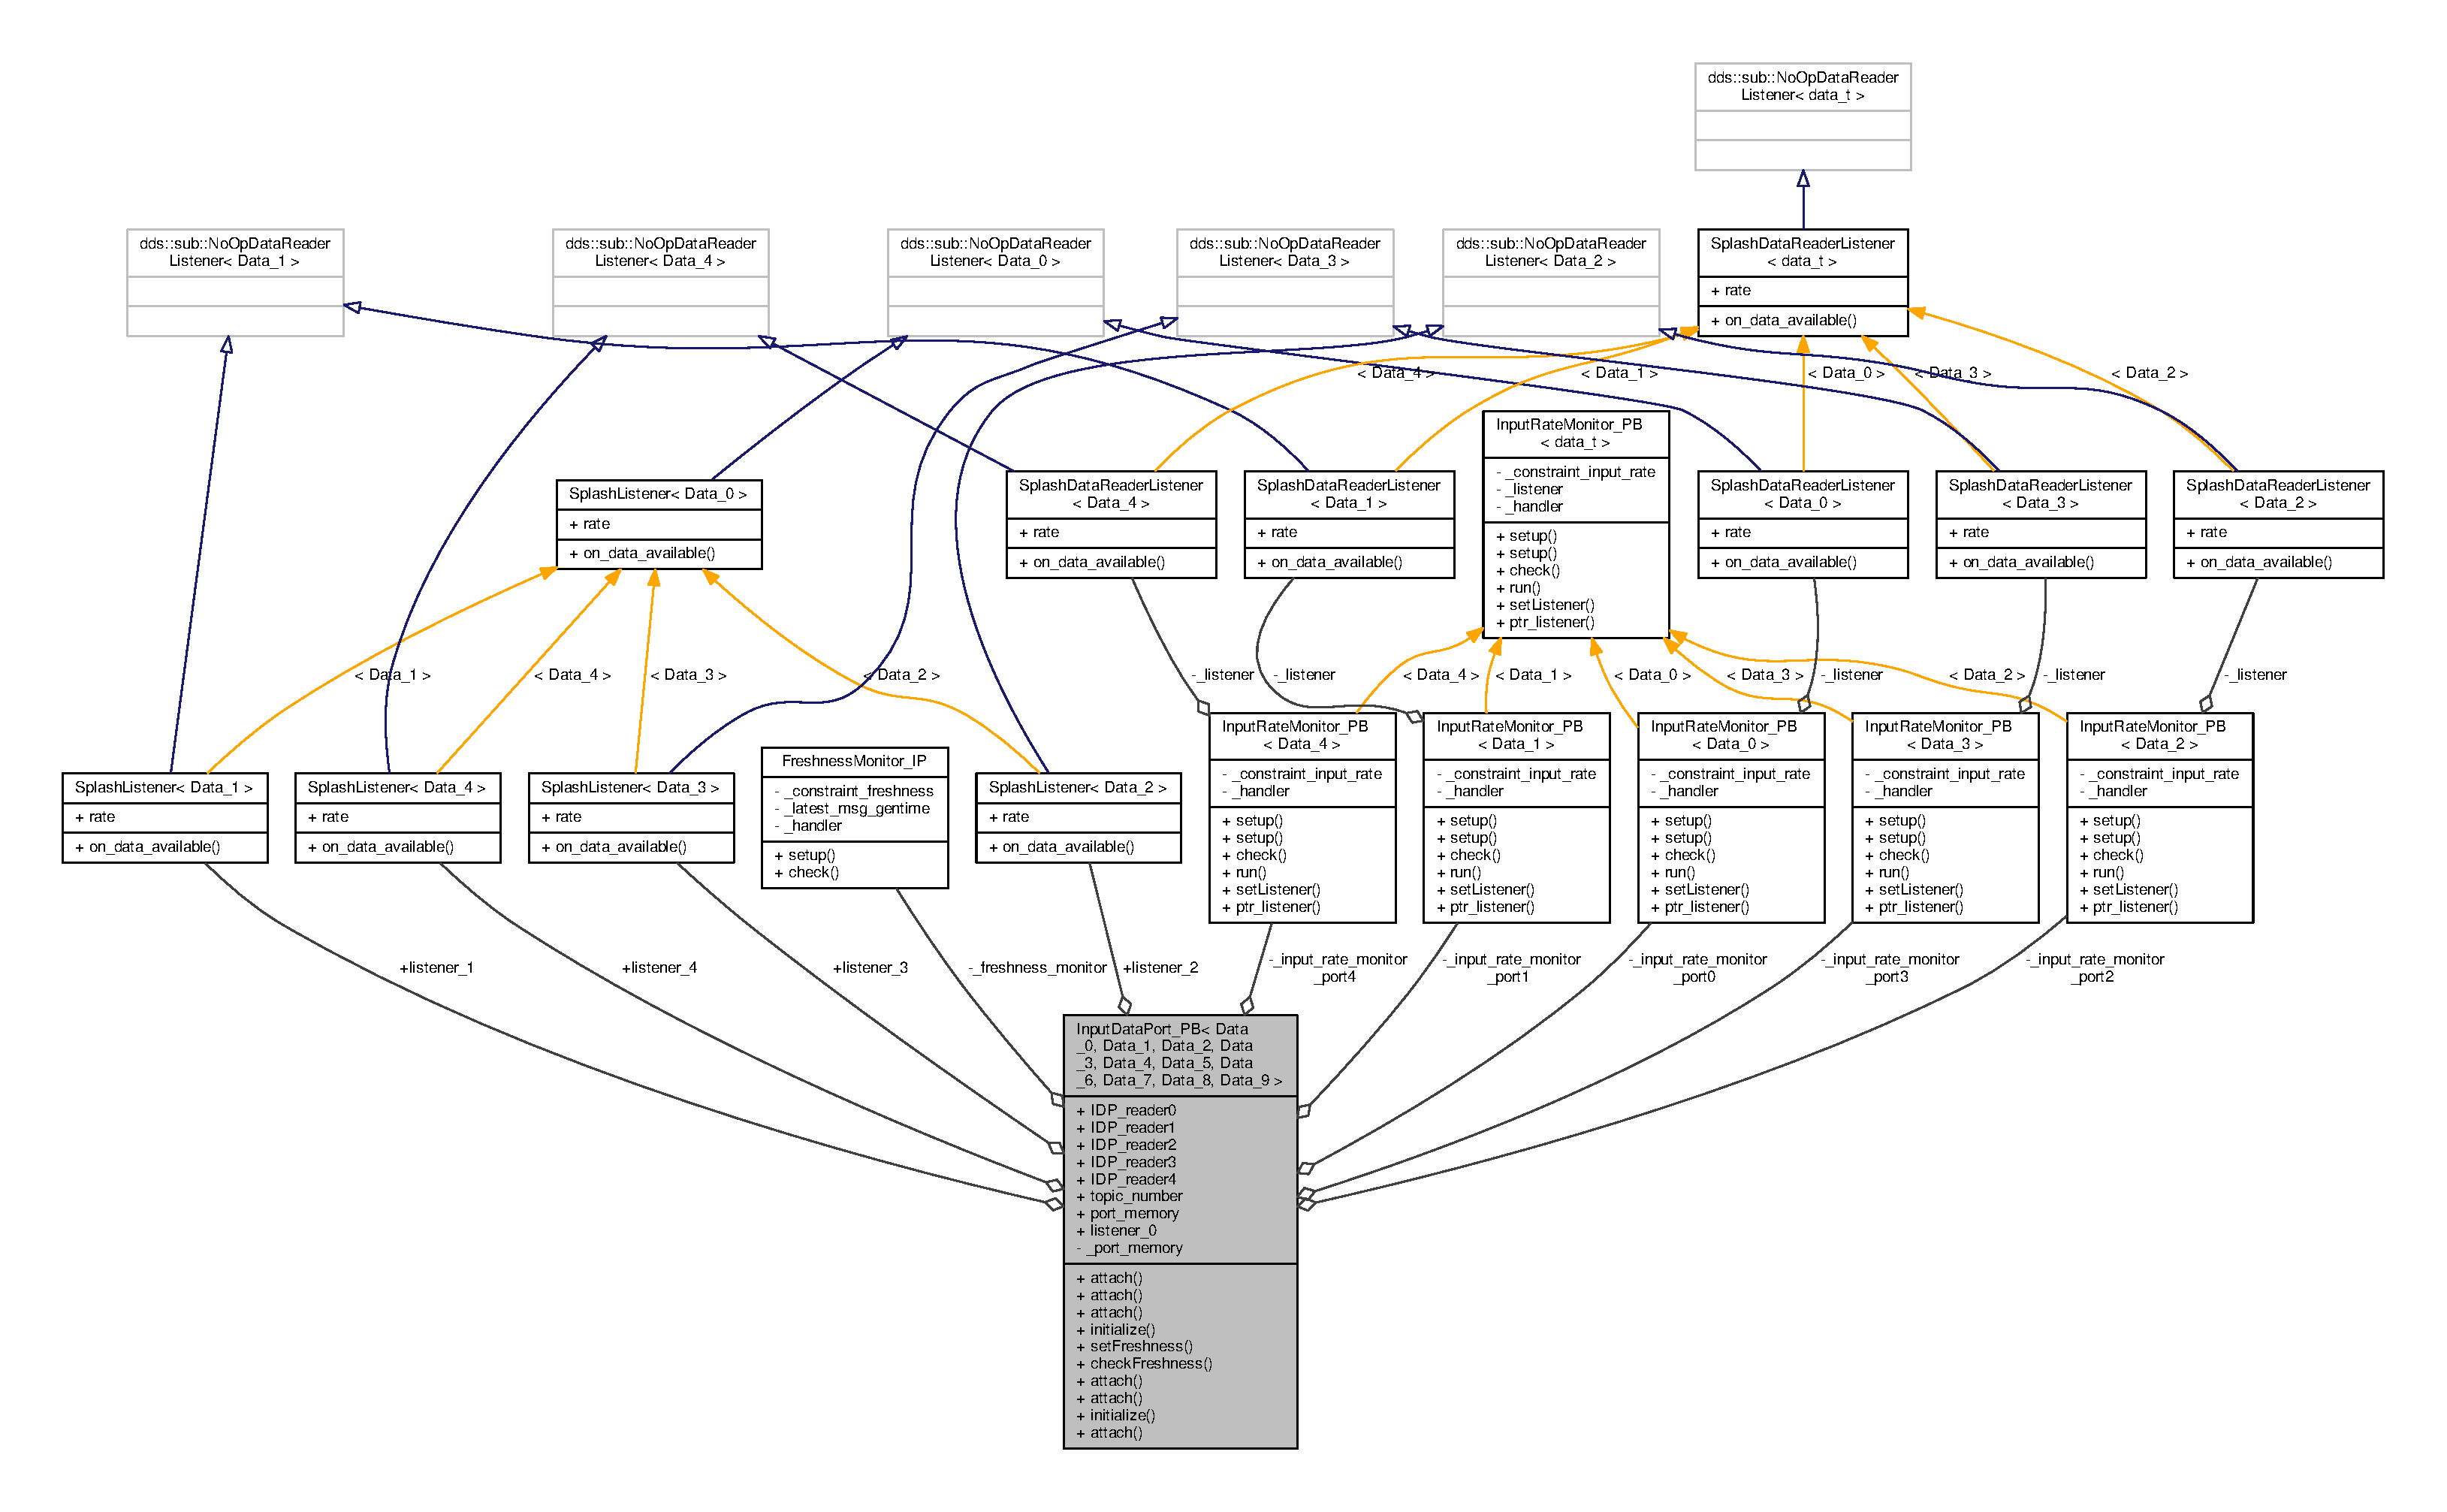
\includegraphics[width=350pt]{classInputDataPort__PB__coll__graph}
\end{center}
\end{figure}
\subsection*{Public 멤버 함수}
\begin{DoxyCompactItemize}
\item 
int \hyperlink{classInputDataPort__PB_a1e2a0dd2fc47211496927695a511e1a5}{attach} (\hyperlink{classProcessingBlock}{Processing\+Block}$<$ Data\+\_\+0, Data\+\_\+1, Data\+\_\+2, Data\+\_\+3, Data\+\_\+4, Data\+\_\+5, Data\+\_\+6, Data\+\_\+7, Data\+\_\+8, Data\+\_\+9 $>$ $\ast$, std\+::string, int)
\item 
int \hyperlink{classInputDataPort__PB_a1e2a0dd2fc47211496927695a511e1a5}{attach} (\hyperlink{classProcessingBlock}{Processing\+Block}$<$ Data\+\_\+0, Data\+\_\+1, Data\+\_\+2, Data\+\_\+3, Data\+\_\+4, Data\+\_\+5, Data\+\_\+6, Data\+\_\+7, Data\+\_\+8, Data\+\_\+9 $>$ $\ast$, std\+::string, int)
\item 
int \hyperlink{classInputDataPort__PB_a1e2a0dd2fc47211496927695a511e1a5}{attach} (\hyperlink{classProcessingBlock}{Processing\+Block}$<$ Data\+\_\+0, Data\+\_\+1, Data\+\_\+2, Data\+\_\+3, Data\+\_\+4, Data\+\_\+5, Data\+\_\+6, Data\+\_\+7, Data\+\_\+8, Data\+\_\+9 $>$ $\ast$, std\+::string, int)
\item 
void \hyperlink{classInputDataPort__PB_a86f4f5662cd09fab17a1027815a2aaa3}{initialize} (int rate, void($\ast$rate\+\_\+handler)(), int freshness, void($\ast$\hyperlink{sample__main_8cpp_ae2b580f894f38496da91bce6c31e186f}{freshness\+\_\+handler})(), bool queueing, int queue\+\_\+size)
\item 
void \hyperlink{classInputDataPort__PB_afc60b73a230f505302984dd8421db791}{set\+Freshness} (int64\+\_\+t freshness, void($\ast$\hyperlink{sample__main_8cpp_ae2b580f894f38496da91bce6c31e186f}{freshness\+\_\+handler})())
\item 
void \hyperlink{classInputDataPort__PB_a43ed8a54ce27b50a0ac8a33f1f93e938}{check\+Freshness} (int64\+\_\+t msg\+\_\+gentime)
\item 
int \hyperlink{classInputDataPort__PB_a1e2a0dd2fc47211496927695a511e1a5}{attach} (\hyperlink{classProcessingBlock}{Processing\+Block}$<$ Data\+\_\+0, Data\+\_\+1, Data\+\_\+2, Data\+\_\+3, Data\+\_\+4, Data\+\_\+5, Data\+\_\+6, Data\+\_\+7, Data\+\_\+8, Data\+\_\+9 $>$ $\ast$, std\+::string, int)
\item 
int \hyperlink{classInputDataPort__PB_a1e2a0dd2fc47211496927695a511e1a5}{attach} (\hyperlink{classProcessingBlock}{Processing\+Block}$<$ Data\+\_\+0, Data\+\_\+1, Data\+\_\+2, Data\+\_\+3, Data\+\_\+4, Data\+\_\+5, Data\+\_\+6, Data\+\_\+7, Data\+\_\+8, Data\+\_\+9 $>$ $\ast$, std\+::string, int)
\item 
void \hyperlink{classInputDataPort__PB_a82f95db8959ef080941612f64620c8c7}{initialize} (int, void($\ast$rate\+\_\+handler)(), int, void($\ast$\hyperlink{sample__main_8cpp_ae2b580f894f38496da91bce6c31e186f}{freshness\+\_\+handler})(), bool, int)
\item 
int \hyperlink{classInputDataPort__PB_a1e2a0dd2fc47211496927695a511e1a5}{attach} (\hyperlink{classProcessingBlock}{Processing\+Block}$<$ Data\+\_\+0, Data\+\_\+1, Data\+\_\+2, Data\+\_\+3, Data\+\_\+4, Data\+\_\+5, Data\+\_\+6, Data\+\_\+7, Data\+\_\+8, Data\+\_\+9 $>$ $\ast$, std\+::string, int)
\end{DoxyCompactItemize}
\subsection*{Public 속성}
\begin{DoxyCompactItemize}
\item 
dds\+::sub\+::\+Data\+Reader$<$ Data\+\_\+0 $>$ $\ast$ \hyperlink{classInputDataPort__PB_ad5db737ed9b58633643a0595cd476083}{I\+D\+P\+\_\+reader0}
\item 
dds\+::sub\+::\+Data\+Reader$<$ Data\+\_\+1 $>$ $\ast$ \hyperlink{classInputDataPort__PB_a70658e2c639e868dc0524b4f97c09da8}{I\+D\+P\+\_\+reader1}
\item 
dds\+::sub\+::\+Data\+Reader$<$ Data\+\_\+2 $>$ $\ast$ \hyperlink{classInputDataPort__PB_a63c8784d2ee1568f704a11e4eea03ca6}{I\+D\+P\+\_\+reader2}
\item 
dds\+::sub\+::\+Data\+Reader$<$ Data\+\_\+3 $>$ $\ast$ \hyperlink{classInputDataPort__PB_a59119679d668507d06016fb12640c80c}{I\+D\+P\+\_\+reader3}
\item 
dds\+::sub\+::\+Data\+Reader$<$ Data\+\_\+4 $>$ $\ast$ \hyperlink{classInputDataPort__PB_aeb99473c8a874344cd133be87607bad2}{I\+D\+P\+\_\+reader4}
\item 
int \hyperlink{classInputDataPort__PB_ae994da4cf26fd15afa7e3c6ac90aa159}{topic\+\_\+number} =0
\item 
void $\ast$ \hyperlink{classInputDataPort__PB_a3f273b7df3b5eb322a422a7d8b80a05f}{port\+\_\+memory}
\item 
\hyperlink{classSplashListener}{Splash\+Listener}$<$ Data\+\_\+0 $>$ $\ast$ \hyperlink{classInputDataPort__PB_a77b666d75615c4284e2e894e2a93d0ce}{listener\+\_\+0}
\item 
\hyperlink{classSplashListener}{Splash\+Listener}$<$ Data\+\_\+1 $>$ $\ast$ \hyperlink{classInputDataPort__PB_acb665e197ba9b211af65cd591467ba66}{listener\+\_\+1}
\item 
\hyperlink{classSplashListener}{Splash\+Listener}$<$ Data\+\_\+2 $>$ $\ast$ \hyperlink{classInputDataPort__PB_af24e1027929b9fd004b1498b54e6173c}{listener\+\_\+2}
\item 
\hyperlink{classSplashListener}{Splash\+Listener}$<$ Data\+\_\+3 $>$ $\ast$ \hyperlink{classInputDataPort__PB_a3045eef4ff7effbb5a8fbfb7552dbb03}{listener\+\_\+3}
\item 
\hyperlink{classSplashListener}{Splash\+Listener}$<$ Data\+\_\+4 $>$ $\ast$ \hyperlink{classInputDataPort__PB_a89c99b63027e15f821a9859d3b988173}{listener\+\_\+4}
\end{DoxyCompactItemize}
\subsection*{Private 속성}
\begin{DoxyCompactItemize}
\item 
\hyperlink{classFreshnessMonitor__IP}{Freshness\+Monitor\+\_\+\+IP} \hyperlink{classInputDataPort__PB_a38da6f4f194f3849420cdbcc5db2019a}{\+\_\+freshness\+\_\+monitor}
\item 
\hyperlink{classInputRateMonitor__PB}{Input\+Rate\+Monitor\+\_\+\+PB}$<$ Data\+\_\+0 $>$ \hyperlink{classInputDataPort__PB_a652aab9b8981a0286167871600a11669}{\+\_\+input\+\_\+rate\+\_\+monitor\+\_\+port0}
\item 
\hyperlink{classInputRateMonitor__PB}{Input\+Rate\+Monitor\+\_\+\+PB}$<$ Data\+\_\+1 $>$ \hyperlink{classInputDataPort__PB_acd3a6668805ad1a581ab741faa3245f1}{\+\_\+input\+\_\+rate\+\_\+monitor\+\_\+port1}
\item 
\hyperlink{classInputRateMonitor__PB}{Input\+Rate\+Monitor\+\_\+\+PB}$<$ Data\+\_\+2 $>$ \hyperlink{classInputDataPort__PB_a9e3ee67f17eac2124e134f683292dfc5}{\+\_\+input\+\_\+rate\+\_\+monitor\+\_\+port2}
\item 
\hyperlink{classInputRateMonitor__PB}{Input\+Rate\+Monitor\+\_\+\+PB}$<$ Data\+\_\+3 $>$ \hyperlink{classInputDataPort__PB_aaff08d79fb2328974a0da28ceca55233}{\+\_\+input\+\_\+rate\+\_\+monitor\+\_\+port3}
\item 
\hyperlink{classInputRateMonitor__PB}{Input\+Rate\+Monitor\+\_\+\+PB}$<$ Data\+\_\+4 $>$ \hyperlink{classInputDataPort__PB_a00fa02ed776eae01fea1d37ce51dd4ab}{\+\_\+input\+\_\+rate\+\_\+monitor\+\_\+port4}
\item 
void $\ast$ \hyperlink{classInputDataPort__PB_aef86b1a63f7a759a9ed5c66bb36c6d47}{\+\_\+port\+\_\+memory}
\end{DoxyCompactItemize}


\subsection{상세한 설명}
\subsubsection*{template$<$typename Data\+\_\+0, typename Data\+\_\+1, typename Data\+\_\+2, typename Data\+\_\+3, typename Data\+\_\+4, typename Data\+\_\+5, typename Data\+\_\+6, typename Data\+\_\+7, typename Data\+\_\+8, typename Data\+\_\+9$>$\\*
class Input\+Data\+Port\+\_\+\+P\+B$<$ Data\+\_\+0, Data\+\_\+1, Data\+\_\+2, Data\+\_\+3, Data\+\_\+4, Data\+\_\+5, Data\+\_\+6, Data\+\_\+7, Data\+\_\+8, Data\+\_\+9 $>$}

Splash l\+Lnguage\+Constructs $>$ Port\+Prototype $>$ Receive\+Interface $>$ Input\+Stream\+Port. 

A input data port used by Processing Block in order to receive data \begin{DoxyAuthor}{작성자}
Jaeho Ahn, Beomjoon Yang 
\end{DoxyAuthor}
\begin{DoxyDate}{날짜}
2018-\/10-\/26 
\end{DoxyDate}
\begin{DoxyVersion}{버전}
0.\+0.\+1 
\end{DoxyVersion}


Base\+\_\+cell.\+cpp 파일의 12 번째 라인에서 정의되었습니다.



\subsection{멤버 함수 문서화}
\index{Input\+Data\+Port\+\_\+\+PB@{Input\+Data\+Port\+\_\+\+PB}!attach@{attach}}
\index{attach@{attach}!Input\+Data\+Port\+\_\+\+PB@{Input\+Data\+Port\+\_\+\+PB}}
\subsubsection[{\texorpdfstring{attach(\+Processing\+Block$<$ Data\+\_\+0, Data\+\_\+1, Data\+\_\+2, Data\+\_\+3, Data\+\_\+4, Data\+\_\+5, Data\+\_\+6, Data\+\_\+7, Data\+\_\+8, Data\+\_\+9 $>$ $\ast$, std\+::string, int)}{attach(ProcessingBlock< Data_0, Data_1, Data_2, Data_3, Data_4, Data_5, Data_6, Data_7, Data_8, Data_9 > *, std::string, int)}}]{\setlength{\rightskip}{0pt plus 5cm}template$<$typename Data\+\_\+0, typename Data\+\_\+1, typename Data\+\_\+2, typename Data\+\_\+3, typename Data\+\_\+4, typename Data\+\_\+5, typename Data\+\_\+6, typename Data\+\_\+7, typename Data\+\_\+8, typename Data\+\_\+9$>$ int {\bf Input\+Data\+Port\+\_\+\+PB}$<$ Data\+\_\+0, Data\+\_\+1, Data\+\_\+2, Data\+\_\+3, Data\+\_\+4, Data\+\_\+5, Data\+\_\+6, Data\+\_\+7, Data\+\_\+8, Data\+\_\+9 $>$\+::attach (
\begin{DoxyParamCaption}
\item[{{\bf Processing\+Block}$<$ Data\+\_\+0, Data\+\_\+1, Data\+\_\+2, Data\+\_\+3, Data\+\_\+4, Data\+\_\+5, Data\+\_\+6, Data\+\_\+7, Data\+\_\+8, Data\+\_\+9 $>$ $\ast$}]{, }
\item[{std\+::string}]{, }
\item[{int}]{}
\end{DoxyParamCaption}
)}\hypertarget{classInputDataPort__PB_a1e2a0dd2fc47211496927695a511e1a5}{}\label{classInputDataPort__PB_a1e2a0dd2fc47211496927695a511e1a5}
\index{Input\+Data\+Port\+\_\+\+PB@{Input\+Data\+Port\+\_\+\+PB}!attach@{attach}}
\index{attach@{attach}!Input\+Data\+Port\+\_\+\+PB@{Input\+Data\+Port\+\_\+\+PB}}
\subsubsection[{\texorpdfstring{attach(\+Processing\+Block$<$ Data\+\_\+0, Data\+\_\+1, Data\+\_\+2, Data\+\_\+3, Data\+\_\+4, Data\+\_\+5, Data\+\_\+6, Data\+\_\+7, Data\+\_\+8, Data\+\_\+9 $>$ $\ast$, std\+::string, int)}{attach(ProcessingBlock< Data_0, Data_1, Data_2, Data_3, Data_4, Data_5, Data_6, Data_7, Data_8, Data_9 > *, std::string, int)}}]{\setlength{\rightskip}{0pt plus 5cm}template$<$typename Data\+\_\+0, typename Data\+\_\+1, typename Data\+\_\+2, typename Data\+\_\+3, typename Data\+\_\+4, typename Data\+\_\+5, typename Data\+\_\+6, typename Data\+\_\+7, typename Data\+\_\+8, typename Data\+\_\+9$>$ int {\bf Input\+Data\+Port\+\_\+\+PB}$<$ Data\+\_\+0, Data\+\_\+1, Data\+\_\+2, Data\+\_\+3, Data\+\_\+4, Data\+\_\+5, Data\+\_\+6, Data\+\_\+7, Data\+\_\+8, Data\+\_\+9 $>$\+::attach (
\begin{DoxyParamCaption}
\item[{{\bf Processing\+Block}$<$ Data\+\_\+0, Data\+\_\+1, Data\+\_\+2, Data\+\_\+3, Data\+\_\+4, Data\+\_\+5, Data\+\_\+6, Data\+\_\+7, Data\+\_\+8, Data\+\_\+9 $>$ $\ast$}]{, }
\item[{std\+::string}]{, }
\item[{int}]{}
\end{DoxyParamCaption}
)}\hypertarget{classInputDataPort__PB_a1e2a0dd2fc47211496927695a511e1a5}{}\label{classInputDataPort__PB_a1e2a0dd2fc47211496927695a511e1a5}
\index{Input\+Data\+Port\+\_\+\+PB@{Input\+Data\+Port\+\_\+\+PB}!attach@{attach}}
\index{attach@{attach}!Input\+Data\+Port\+\_\+\+PB@{Input\+Data\+Port\+\_\+\+PB}}
\subsubsection[{\texorpdfstring{attach(\+Processing\+Block$<$ Data\+\_\+0, Data\+\_\+1, Data\+\_\+2, Data\+\_\+3, Data\+\_\+4, Data\+\_\+5, Data\+\_\+6, Data\+\_\+7, Data\+\_\+8, Data\+\_\+9 $>$ $\ast$, std\+::string, int)}{attach(ProcessingBlock< Data_0, Data_1, Data_2, Data_3, Data_4, Data_5, Data_6, Data_7, Data_8, Data_9 > *, std::string, int)}}]{\setlength{\rightskip}{0pt plus 5cm}template$<$typename Data\+\_\+0 , typename Data\+\_\+1 , typename Data\+\_\+2 , typename Data\+\_\+3 , typename Data\+\_\+4 , typename Data\+\_\+5 , typename Data\+\_\+6 , typename Data\+\_\+7 , typename Data\+\_\+8 , typename Data\+\_\+9 $>$ int {\bf Input\+Data\+Port\+\_\+\+PB}$<$ Data\+\_\+0, Data\+\_\+1, Data\+\_\+2, Data\+\_\+3, Data\+\_\+4, Data\+\_\+5, Data\+\_\+6, Data\+\_\+7, Data\+\_\+8, Data\+\_\+9 $>$\+::attach (
\begin{DoxyParamCaption}
\item[{{\bf Processing\+Block}$<$ Data\+\_\+0, Data\+\_\+1, Data\+\_\+2, Data\+\_\+3, Data\+\_\+4, Data\+\_\+5, Data\+\_\+6, Data\+\_\+7, Data\+\_\+8, Data\+\_\+9 $>$ $\ast$}]{PB, }
\item[{std\+::string}]{topic, }
\item[{int}]{topic\+\_\+number}
\end{DoxyParamCaption}
)}\hypertarget{classInputDataPort__PB_a1e2a0dd2fc47211496927695a511e1a5}{}\label{classInputDataPort__PB_a1e2a0dd2fc47211496927695a511e1a5}


Base\+\_\+cell.\+cpp 파일의 205 번째 라인에서 정의되었습니다.



다음을 참조함 \+:  Processing\+Block$<$ Data\+\_\+0, Data\+\_\+1, Data\+\_\+2, Data\+\_\+3, Data\+\_\+4, Data\+\_\+5, Data\+\_\+6, Data\+\_\+7, Data\+\_\+8, Data\+\_\+9 $>$\+::\+I\+D\+P0, Processing\+Block$<$ Data\+\_\+0, Data\+\_\+1, Data\+\_\+2, Data\+\_\+3, Data\+\_\+4, Data\+\_\+5, Data\+\_\+6, Data\+\_\+7, Data\+\_\+8, Data\+\_\+9 $>$\+::\+I\+D\+P1, Processing\+Block$<$ Data\+\_\+0, Data\+\_\+1, Data\+\_\+2, Data\+\_\+3, Data\+\_\+4, Data\+\_\+5, Data\+\_\+6, Data\+\_\+7, Data\+\_\+8, Data\+\_\+9 $>$\+::\+I\+D\+P2, Processing\+Block$<$ Data\+\_\+0, Data\+\_\+1, Data\+\_\+2, Data\+\_\+3, Data\+\_\+4, Data\+\_\+5, Data\+\_\+6, Data\+\_\+7, Data\+\_\+8, Data\+\_\+9 $>$\+::\+I\+D\+P3, Processing\+Block$<$ Data\+\_\+0, Data\+\_\+1, Data\+\_\+2, Data\+\_\+3, Data\+\_\+4, Data\+\_\+5, Data\+\_\+6, Data\+\_\+7, Data\+\_\+8, Data\+\_\+9 $>$\+::\+I\+D\+P4, Processing\+Block$<$ Data\+\_\+0, Data\+\_\+1, Data\+\_\+2, Data\+\_\+3, Data\+\_\+4, Data\+\_\+5, Data\+\_\+6, Data\+\_\+7, Data\+\_\+8, Data\+\_\+9 $>$\+::topic0, Processing\+Block$<$ Data\+\_\+0, Data\+\_\+1, Data\+\_\+2, Data\+\_\+3, Data\+\_\+4, Data\+\_\+5, Data\+\_\+6, Data\+\_\+7, Data\+\_\+8, Data\+\_\+9 $>$\+::topic1, Processing\+Block$<$ Data\+\_\+0, Data\+\_\+1, Data\+\_\+2, Data\+\_\+3, Data\+\_\+4, Data\+\_\+5, Data\+\_\+6, Data\+\_\+7, Data\+\_\+8, Data\+\_\+9 $>$\+::topic2, Processing\+Block$<$ Data\+\_\+0, Data\+\_\+1, Data\+\_\+2, Data\+\_\+3, Data\+\_\+4, Data\+\_\+5, Data\+\_\+6, Data\+\_\+7, Data\+\_\+8, Data\+\_\+9 $>$\+::topic3, Processing\+Block$<$ Data\+\_\+0, Data\+\_\+1, Data\+\_\+2, Data\+\_\+3, Data\+\_\+4, Data\+\_\+5, Data\+\_\+6, Data\+\_\+7, Data\+\_\+8, Data\+\_\+9 $>$\+::topic4.



다음에 의해서 참조됨 \+:  Input\+Data\+Port\+\_\+\+P\+B$<$ Data\+\_\+0, Data\+\_\+1, Data\+\_\+2, Data\+\_\+3, Data\+\_\+4, Data\+\_\+5, Data\+\_\+6, Data\+\_\+7, Data\+\_\+8, Data\+\_\+9 $>$\+::check\+Freshness(), main().



이 함수를 호출하는 함수들에 대한 그래프입니다.\+:\nopagebreak
\begin{figure}[H]
\begin{center}
\leavevmode
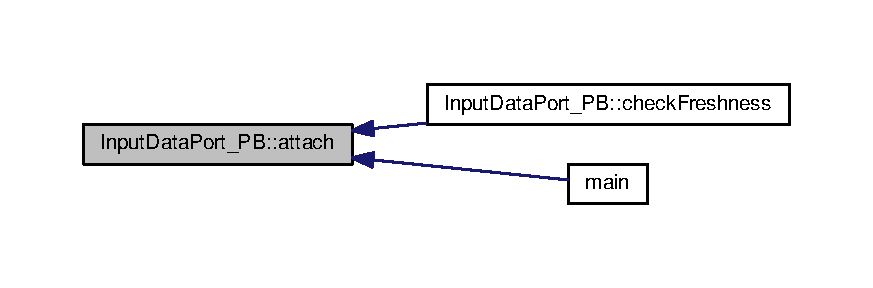
\includegraphics[width=350pt]{classInputDataPort__PB_a1e2a0dd2fc47211496927695a511e1a5_icgraph}
\end{center}
\end{figure}


\index{Input\+Data\+Port\+\_\+\+PB@{Input\+Data\+Port\+\_\+\+PB}!attach@{attach}}
\index{attach@{attach}!Input\+Data\+Port\+\_\+\+PB@{Input\+Data\+Port\+\_\+\+PB}}
\subsubsection[{\texorpdfstring{attach(\+Processing\+Block$<$ Data\+\_\+0, Data\+\_\+1, Data\+\_\+2, Data\+\_\+3, Data\+\_\+4, Data\+\_\+5, Data\+\_\+6, Data\+\_\+7, Data\+\_\+8, Data\+\_\+9 $>$ $\ast$, std\+::string, int)}{attach(ProcessingBlock< Data_0, Data_1, Data_2, Data_3, Data_4, Data_5, Data_6, Data_7, Data_8, Data_9 > *, std::string, int)}}]{\setlength{\rightskip}{0pt plus 5cm}template$<$typename Data\+\_\+0, typename Data\+\_\+1, typename Data\+\_\+2, typename Data\+\_\+3, typename Data\+\_\+4, typename Data\+\_\+5, typename Data\+\_\+6, typename Data\+\_\+7, typename Data\+\_\+8, typename Data\+\_\+9$>$ int {\bf Input\+Data\+Port\+\_\+\+PB}$<$ Data\+\_\+0, Data\+\_\+1, Data\+\_\+2, Data\+\_\+3, Data\+\_\+4, Data\+\_\+5, Data\+\_\+6, Data\+\_\+7, Data\+\_\+8, Data\+\_\+9 $>$\+::attach (
\begin{DoxyParamCaption}
\item[{{\bf Processing\+Block}$<$ Data\+\_\+0, Data\+\_\+1, Data\+\_\+2, Data\+\_\+3, Data\+\_\+4, Data\+\_\+5, Data\+\_\+6, Data\+\_\+7, Data\+\_\+8, Data\+\_\+9 $>$ $\ast$}]{, }
\item[{std\+::string}]{, }
\item[{int}]{}
\end{DoxyParamCaption}
)}\hypertarget{classInputDataPort__PB_a1e2a0dd2fc47211496927695a511e1a5}{}\label{classInputDataPort__PB_a1e2a0dd2fc47211496927695a511e1a5}
\index{Input\+Data\+Port\+\_\+\+PB@{Input\+Data\+Port\+\_\+\+PB}!attach@{attach}}
\index{attach@{attach}!Input\+Data\+Port\+\_\+\+PB@{Input\+Data\+Port\+\_\+\+PB}}
\subsubsection[{\texorpdfstring{attach(\+Processing\+Block$<$ Data\+\_\+0, Data\+\_\+1, Data\+\_\+2, Data\+\_\+3, Data\+\_\+4, Data\+\_\+5, Data\+\_\+6, Data\+\_\+7, Data\+\_\+8, Data\+\_\+9 $>$ $\ast$, std\+::string, int)}{attach(ProcessingBlock< Data_0, Data_1, Data_2, Data_3, Data_4, Data_5, Data_6, Data_7, Data_8, Data_9 > *, std::string, int)}}]{\setlength{\rightskip}{0pt plus 5cm}template$<$typename Data\+\_\+0, typename Data\+\_\+1, typename Data\+\_\+2, typename Data\+\_\+3, typename Data\+\_\+4, typename Data\+\_\+5, typename Data\+\_\+6, typename Data\+\_\+7, typename Data\+\_\+8, typename Data\+\_\+9$>$ int {\bf Input\+Data\+Port\+\_\+\+PB}$<$ Data\+\_\+0, Data\+\_\+1, Data\+\_\+2, Data\+\_\+3, Data\+\_\+4, Data\+\_\+5, Data\+\_\+6, Data\+\_\+7, Data\+\_\+8, Data\+\_\+9 $>$\+::attach (
\begin{DoxyParamCaption}
\item[{{\bf Processing\+Block}$<$ Data\+\_\+0, Data\+\_\+1, Data\+\_\+2, Data\+\_\+3, Data\+\_\+4, Data\+\_\+5, Data\+\_\+6, Data\+\_\+7, Data\+\_\+8, Data\+\_\+9 $>$ $\ast$}]{, }
\item[{std\+::string}]{, }
\item[{int}]{}
\end{DoxyParamCaption}
)}\hypertarget{classInputDataPort__PB_a1e2a0dd2fc47211496927695a511e1a5}{}\label{classInputDataPort__PB_a1e2a0dd2fc47211496927695a511e1a5}
\index{Input\+Data\+Port\+\_\+\+PB@{Input\+Data\+Port\+\_\+\+PB}!attach@{attach}}
\index{attach@{attach}!Input\+Data\+Port\+\_\+\+PB@{Input\+Data\+Port\+\_\+\+PB}}
\subsubsection[{\texorpdfstring{attach(\+Processing\+Block$<$ Data\+\_\+0, Data\+\_\+1, Data\+\_\+2, Data\+\_\+3, Data\+\_\+4, Data\+\_\+5, Data\+\_\+6, Data\+\_\+7, Data\+\_\+8, Data\+\_\+9 $>$ $\ast$, std\+::string, int)}{attach(ProcessingBlock< Data_0, Data_1, Data_2, Data_3, Data_4, Data_5, Data_6, Data_7, Data_8, Data_9 > *, std::string, int)}}]{\setlength{\rightskip}{0pt plus 5cm}template$<$typename Data\+\_\+0, typename Data\+\_\+1, typename Data\+\_\+2, typename Data\+\_\+3, typename Data\+\_\+4, typename Data\+\_\+5, typename Data\+\_\+6, typename Data\+\_\+7, typename Data\+\_\+8, typename Data\+\_\+9$>$ int {\bf Input\+Data\+Port\+\_\+\+PB}$<$ Data\+\_\+0, Data\+\_\+1, Data\+\_\+2, Data\+\_\+3, Data\+\_\+4, Data\+\_\+5, Data\+\_\+6, Data\+\_\+7, Data\+\_\+8, Data\+\_\+9 $>$\+::attach (
\begin{DoxyParamCaption}
\item[{{\bf Processing\+Block}$<$ Data\+\_\+0, Data\+\_\+1, Data\+\_\+2, Data\+\_\+3, Data\+\_\+4, Data\+\_\+5, Data\+\_\+6, Data\+\_\+7, Data\+\_\+8, Data\+\_\+9 $>$ $\ast$}]{, }
\item[{std\+::string}]{, }
\item[{int}]{}
\end{DoxyParamCaption}
)}\hypertarget{classInputDataPort__PB_a1e2a0dd2fc47211496927695a511e1a5}{}\label{classInputDataPort__PB_a1e2a0dd2fc47211496927695a511e1a5}
\index{Input\+Data\+Port\+\_\+\+PB@{Input\+Data\+Port\+\_\+\+PB}!check\+Freshness@{check\+Freshness}}
\index{check\+Freshness@{check\+Freshness}!Input\+Data\+Port\+\_\+\+PB@{Input\+Data\+Port\+\_\+\+PB}}
\subsubsection[{\texorpdfstring{check\+Freshness(int64\+\_\+t msg\+\_\+gentime)}{checkFreshness(int64_t msg_gentime)}}]{\setlength{\rightskip}{0pt plus 5cm}template$<$typename Data\+\_\+0 , typename Data\+\_\+1 , typename Data\+\_\+2 , typename Data\+\_\+3 , typename Data\+\_\+4 , typename Data\+\_\+5 , typename Data\+\_\+6 , typename Data\+\_\+7 , typename Data\+\_\+8 , typename Data\+\_\+9 $>$ void {\bf Input\+Data\+Port\+\_\+\+PB}$<$ Data\+\_\+0, Data\+\_\+1, Data\+\_\+2, Data\+\_\+3, Data\+\_\+4, Data\+\_\+5, Data\+\_\+6, Data\+\_\+7, Data\+\_\+8, Data\+\_\+9 $>$\+::check\+Freshness (
\begin{DoxyParamCaption}
\item[{int64\+\_\+t}]{msg\+\_\+gentime}
\end{DoxyParamCaption}
)}\hypertarget{classInputDataPort__PB_a43ed8a54ce27b50a0ac8a33f1f93e938}{}\label{classInputDataPort__PB_a43ed8a54ce27b50a0ac8a33f1f93e938}


Processing\+\_\+block.\+cpp 파일의 696 번째 라인에서 정의되었습니다.



다음을 참조함 \+:  Input\+Data\+Port\+\_\+\+P\+B$<$ Data\+\_\+0, Data\+\_\+1, Data\+\_\+2, Data\+\_\+3, Data\+\_\+4, Data\+\_\+5, Data\+\_\+6, Data\+\_\+7, Data\+\_\+8, Data\+\_\+9 $>$\+::attach(), Freshness\+Monitor\+\_\+\+I\+P\+::check(), Processing\+Block$<$ Data\+\_\+0, Data\+\_\+1, Data\+\_\+2, Data\+\_\+3, Data\+\_\+4, Data\+\_\+5, Data\+\_\+6, Data\+\_\+7, Data\+\_\+8, Data\+\_\+9 $>$\+::\+I\+D\+P0, Processing\+Block$<$ Data\+\_\+0, Data\+\_\+1, Data\+\_\+2, Data\+\_\+3, Data\+\_\+4, Data\+\_\+5, Data\+\_\+6, Data\+\_\+7, Data\+\_\+8, Data\+\_\+9 $>$\+::\+I\+D\+P1, Processing\+Block$<$ Data\+\_\+0, Data\+\_\+1, Data\+\_\+2, Data\+\_\+3, Data\+\_\+4, Data\+\_\+5, Data\+\_\+6, Data\+\_\+7, Data\+\_\+8, Data\+\_\+9 $>$\+::\+I\+D\+P2, Processing\+Block$<$ Data\+\_\+0, Data\+\_\+1, Data\+\_\+2, Data\+\_\+3, Data\+\_\+4, Data\+\_\+5, Data\+\_\+6, Data\+\_\+7, Data\+\_\+8, Data\+\_\+9 $>$\+::\+I\+D\+P3, Processing\+Block$<$ Data\+\_\+0, Data\+\_\+1, Data\+\_\+2, Data\+\_\+3, Data\+\_\+4, Data\+\_\+5, Data\+\_\+6, Data\+\_\+7, Data\+\_\+8, Data\+\_\+9 $>$\+::\+I\+D\+P4, Input\+Rate\+Monitor\+\_\+\+P\+B$<$ data\+\_\+t $>$\+::ptr\+\_\+listener(), Input\+Rate\+Monitor\+\_\+\+P\+B$<$ data\+\_\+t $>$\+::set\+Listener(), Processing\+Block$<$ Data\+\_\+0, Data\+\_\+1, Data\+\_\+2, Data\+\_\+3, Data\+\_\+4, Data\+\_\+5, Data\+\_\+6, Data\+\_\+7, Data\+\_\+8, Data\+\_\+9 $>$\+::topic0, Processing\+Block$<$ Data\+\_\+0, Data\+\_\+1, Data\+\_\+2, Data\+\_\+3, Data\+\_\+4, Data\+\_\+5, Data\+\_\+6, Data\+\_\+7, Data\+\_\+8, Data\+\_\+9 $>$\+::topic1, Processing\+Block$<$ Data\+\_\+0, Data\+\_\+1, Data\+\_\+2, Data\+\_\+3, Data\+\_\+4, Data\+\_\+5, Data\+\_\+6, Data\+\_\+7, Data\+\_\+8, Data\+\_\+9 $>$\+::topic2, Processing\+Block$<$ Data\+\_\+0, Data\+\_\+1, Data\+\_\+2, Data\+\_\+3, Data\+\_\+4, Data\+\_\+5, Data\+\_\+6, Data\+\_\+7, Data\+\_\+8, Data\+\_\+9 $>$\+::topic3, Processing\+Block$<$ Data\+\_\+0, Data\+\_\+1, Data\+\_\+2, Data\+\_\+3, Data\+\_\+4, Data\+\_\+5, Data\+\_\+6, Data\+\_\+7, Data\+\_\+8, Data\+\_\+9 $>$\+::topic4.



이 함수 내부에서 호출하는 함수들에 대한 그래프입니다.\+:\nopagebreak
\begin{figure}[H]
\begin{center}
\leavevmode
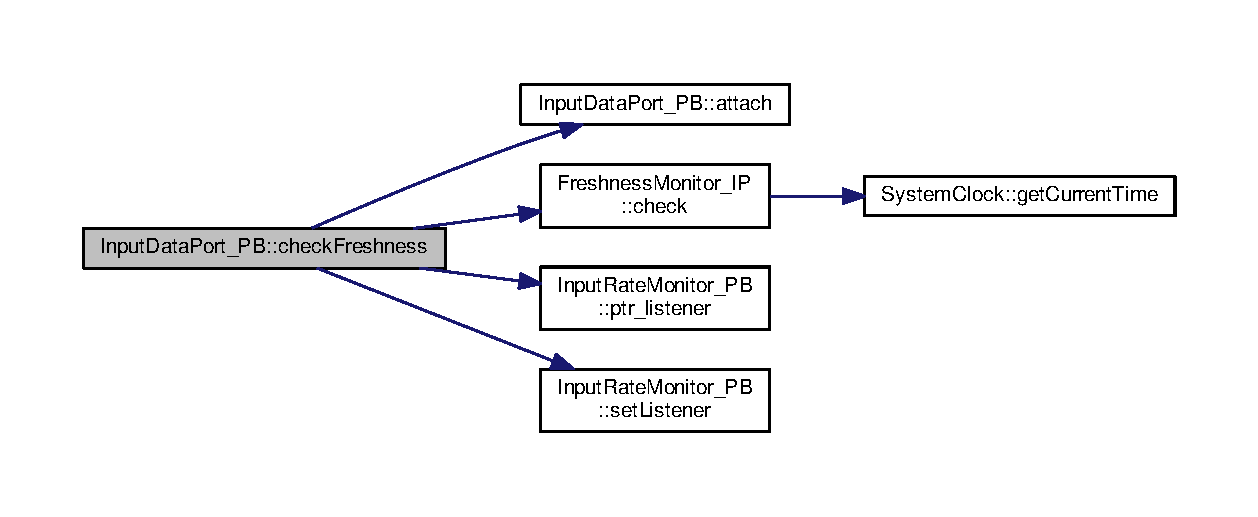
\includegraphics[width=350pt]{classInputDataPort__PB_a43ed8a54ce27b50a0ac8a33f1f93e938_cgraph}
\end{center}
\end{figure}


\index{Input\+Data\+Port\+\_\+\+PB@{Input\+Data\+Port\+\_\+\+PB}!initialize@{initialize}}
\index{initialize@{initialize}!Input\+Data\+Port\+\_\+\+PB@{Input\+Data\+Port\+\_\+\+PB}}
\subsubsection[{\texorpdfstring{initialize(int, void($\ast$rate\+\_\+handler)(), int, void($\ast$freshness\+\_\+handler)(), bool, int)}{initialize(int, void(*rate_handler)(), int, void(*freshness_handler)(), bool, int)}}]{\setlength{\rightskip}{0pt plus 5cm}template$<$typename Data\+\_\+0, typename Data\+\_\+1, typename Data\+\_\+2, typename Data\+\_\+3, typename Data\+\_\+4, typename Data\+\_\+5, typename Data\+\_\+6, typename Data\+\_\+7, typename Data\+\_\+8, typename Data\+\_\+9$>$ void {\bf Input\+Data\+Port\+\_\+\+PB}$<$ Data\+\_\+0, Data\+\_\+1, Data\+\_\+2, Data\+\_\+3, Data\+\_\+4, Data\+\_\+5, Data\+\_\+6, Data\+\_\+7, Data\+\_\+8, Data\+\_\+9 $>$\+::initialize (
\begin{DoxyParamCaption}
\item[{int}]{, }
\item[{void($\ast$)()}]{rate\+\_\+handler, }
\item[{int}]{, }
\item[{void($\ast$)()}]{freshness\+\_\+handler, }
\item[{bool}]{, }
\item[{int}]{}
\end{DoxyParamCaption}
)}\hypertarget{classInputDataPort__PB_a82f95db8959ef080941612f64620c8c7}{}\label{classInputDataPort__PB_a82f95db8959ef080941612f64620c8c7}
\index{Input\+Data\+Port\+\_\+\+PB@{Input\+Data\+Port\+\_\+\+PB}!initialize@{initialize}}
\index{initialize@{initialize}!Input\+Data\+Port\+\_\+\+PB@{Input\+Data\+Port\+\_\+\+PB}}
\subsubsection[{\texorpdfstring{initialize(int rate, void($\ast$rate\+\_\+handler)(), int freshness, void($\ast$freshness\+\_\+handler)(), bool queueing, int queue\+\_\+size)}{initialize(int rate, void(*rate_handler)(), int freshness, void(*freshness_handler)(), bool queueing, int queue_size)}}]{\setlength{\rightskip}{0pt plus 5cm}template$<$typename Data\+\_\+0 , typename Data\+\_\+1 , typename Data\+\_\+2 , typename Data\+\_\+3 , typename Data\+\_\+4 , typename Data\+\_\+5 , typename Data\+\_\+6 , typename Data\+\_\+7 , typename Data\+\_\+8 , typename Data\+\_\+9 $>$ void {\bf Input\+Data\+Port\+\_\+\+PB}$<$ Data\+\_\+0, Data\+\_\+1, Data\+\_\+2, Data\+\_\+3, Data\+\_\+4, Data\+\_\+5, Data\+\_\+6, Data\+\_\+7, Data\+\_\+8, Data\+\_\+9 $>$\+::initialize (
\begin{DoxyParamCaption}
\item[{int}]{rate, }
\item[{void($\ast$)()}]{rate\+\_\+handler, }
\item[{int}]{freshness, }
\item[{void($\ast$)()}]{freshness\+\_\+handler, }
\item[{bool}]{queueing, }
\item[{int}]{queue\+\_\+size}
\end{DoxyParamCaption}
)}\hypertarget{classInputDataPort__PB_a86f4f5662cd09fab17a1027815a2aaa3}{}\label{classInputDataPort__PB_a86f4f5662cd09fab17a1027815a2aaa3}


Processing\+\_\+block.\+cpp 파일의 801 번째 라인에서 정의되었습니다.



다음을 참조함 \+:  freshness\+\_\+handler(), Input\+Rate\+Monitor\+\_\+\+P\+B$<$ data\+\_\+t $>$\+::run(), Input\+Rate\+Monitor\+\_\+\+P\+B$<$ data\+\_\+t $>$\+::setup().



다음에 의해서 참조됨 \+:  main(), rate\+\_\+check().



이 함수 내부에서 호출하는 함수들에 대한 그래프입니다.\+:\nopagebreak
\begin{figure}[H]
\begin{center}
\leavevmode
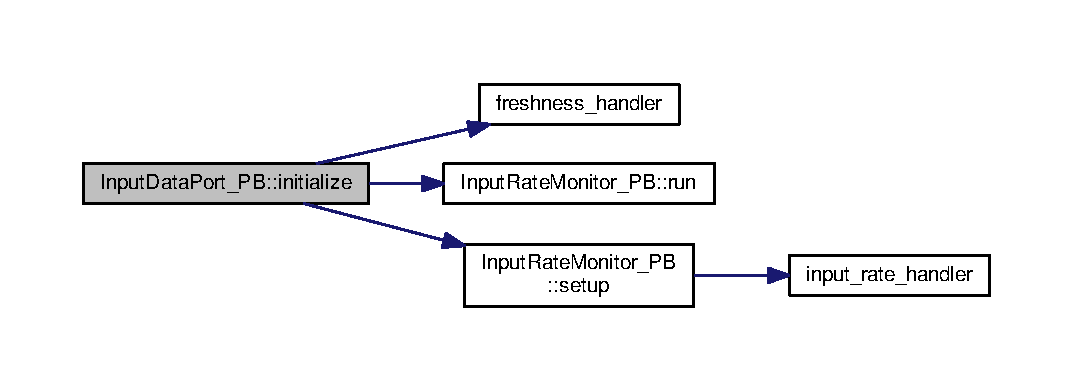
\includegraphics[width=350pt]{classInputDataPort__PB_a86f4f5662cd09fab17a1027815a2aaa3_cgraph}
\end{center}
\end{figure}




이 함수를 호출하는 함수들에 대한 그래프입니다.\+:\nopagebreak
\begin{figure}[H]
\begin{center}
\leavevmode
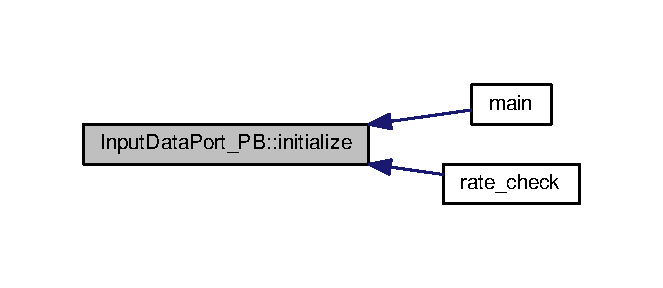
\includegraphics[width=318pt]{classInputDataPort__PB_a86f4f5662cd09fab17a1027815a2aaa3_icgraph}
\end{center}
\end{figure}


\index{Input\+Data\+Port\+\_\+\+PB@{Input\+Data\+Port\+\_\+\+PB}!set\+Freshness@{set\+Freshness}}
\index{set\+Freshness@{set\+Freshness}!Input\+Data\+Port\+\_\+\+PB@{Input\+Data\+Port\+\_\+\+PB}}
\subsubsection[{\texorpdfstring{set\+Freshness(int64\+\_\+t freshness, void($\ast$freshness\+\_\+handler)())}{setFreshness(int64_t freshness, void(*freshness_handler)())}}]{\setlength{\rightskip}{0pt plus 5cm}template$<$typename Data\+\_\+0 , typename Data\+\_\+1 , typename Data\+\_\+2 , typename Data\+\_\+3 , typename Data\+\_\+4 , typename Data\+\_\+5 , typename Data\+\_\+6 , typename Data\+\_\+7 , typename Data\+\_\+8 , typename Data\+\_\+9 $>$ void {\bf Input\+Data\+Port\+\_\+\+PB}$<$ Data\+\_\+0, Data\+\_\+1, Data\+\_\+2, Data\+\_\+3, Data\+\_\+4, Data\+\_\+5, Data\+\_\+6, Data\+\_\+7, Data\+\_\+8, Data\+\_\+9 $>$\+::set\+Freshness (
\begin{DoxyParamCaption}
\item[{int64\+\_\+t}]{freshness, }
\item[{void($\ast$)()}]{freshness\+\_\+handler}
\end{DoxyParamCaption}
)}\hypertarget{classInputDataPort__PB_afc60b73a230f505302984dd8421db791}{}\label{classInputDataPort__PB_afc60b73a230f505302984dd8421db791}


Processing\+\_\+block.\+cpp 파일의 684 번째 라인에서 정의되었습니다.



다음을 참조함 \+:  freshness\+\_\+handler(), Freshness\+Monitor\+\_\+\+I\+P\+::setup().



이 함수 내부에서 호출하는 함수들에 대한 그래프입니다.\+:\nopagebreak
\begin{figure}[H]
\begin{center}
\leavevmode
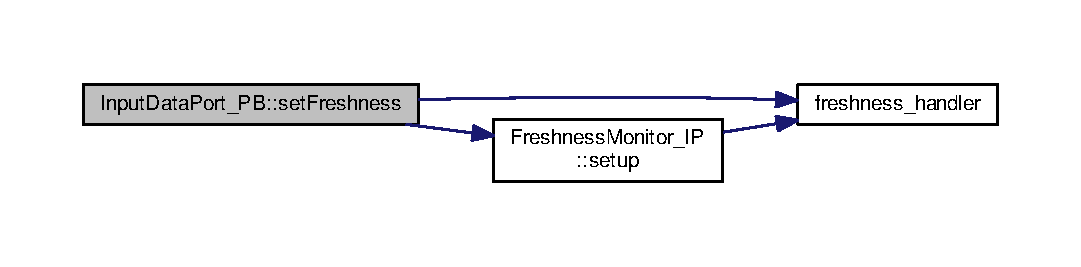
\includegraphics[width=350pt]{classInputDataPort__PB_afc60b73a230f505302984dd8421db791_cgraph}
\end{center}
\end{figure}




\subsection{멤버 데이타 문서화}
\index{Input\+Data\+Port\+\_\+\+PB@{Input\+Data\+Port\+\_\+\+PB}!\+\_\+freshness\+\_\+monitor@{\+\_\+freshness\+\_\+monitor}}
\index{\+\_\+freshness\+\_\+monitor@{\+\_\+freshness\+\_\+monitor}!Input\+Data\+Port\+\_\+\+PB@{Input\+Data\+Port\+\_\+\+PB}}
\subsubsection[{\texorpdfstring{\+\_\+freshness\+\_\+monitor}{_freshness_monitor}}]{\setlength{\rightskip}{0pt plus 5cm}template$<$typename Data\+\_\+0, typename Data\+\_\+1, typename Data\+\_\+2, typename Data\+\_\+3, typename Data\+\_\+4, typename Data\+\_\+5, typename Data\+\_\+6, typename Data\+\_\+7, typename Data\+\_\+8, typename Data\+\_\+9$>$ {\bf Freshness\+Monitor\+\_\+\+IP} {\bf Input\+Data\+Port\+\_\+\+PB}$<$ Data\+\_\+0, Data\+\_\+1, Data\+\_\+2, Data\+\_\+3, Data\+\_\+4, Data\+\_\+5, Data\+\_\+6, Data\+\_\+7, Data\+\_\+8, Data\+\_\+9 $>$\+::\+\_\+freshness\+\_\+monitor\hspace{0.3cm}{\ttfamily [private]}}\hypertarget{classInputDataPort__PB_a38da6f4f194f3849420cdbcc5db2019a}{}\label{classInputDataPort__PB_a38da6f4f194f3849420cdbcc5db2019a}


Processing\+\_\+block.\+cpp 파일의 649 번째 라인에서 정의되었습니다.

\index{Input\+Data\+Port\+\_\+\+PB@{Input\+Data\+Port\+\_\+\+PB}!\+\_\+input\+\_\+rate\+\_\+monitor\+\_\+port0@{\+\_\+input\+\_\+rate\+\_\+monitor\+\_\+port0}}
\index{\+\_\+input\+\_\+rate\+\_\+monitor\+\_\+port0@{\+\_\+input\+\_\+rate\+\_\+monitor\+\_\+port0}!Input\+Data\+Port\+\_\+\+PB@{Input\+Data\+Port\+\_\+\+PB}}
\subsubsection[{\texorpdfstring{\+\_\+input\+\_\+rate\+\_\+monitor\+\_\+port0}{_input_rate_monitor_port0}}]{\setlength{\rightskip}{0pt plus 5cm}template$<$typename Data\+\_\+0, typename Data\+\_\+1, typename Data\+\_\+2, typename Data\+\_\+3, typename Data\+\_\+4, typename Data\+\_\+5, typename Data\+\_\+6, typename Data\+\_\+7, typename Data\+\_\+8, typename Data\+\_\+9$>$ {\bf Input\+Rate\+Monitor\+\_\+\+PB}$<$Data\+\_\+0$>$ {\bf Input\+Data\+Port\+\_\+\+PB}$<$ Data\+\_\+0, Data\+\_\+1, Data\+\_\+2, Data\+\_\+3, Data\+\_\+4, Data\+\_\+5, Data\+\_\+6, Data\+\_\+7, Data\+\_\+8, Data\+\_\+9 $>$\+::\+\_\+input\+\_\+rate\+\_\+monitor\+\_\+port0\hspace{0.3cm}{\ttfamily [private]}}\hypertarget{classInputDataPort__PB_a652aab9b8981a0286167871600a11669}{}\label{classInputDataPort__PB_a652aab9b8981a0286167871600a11669}


Processing\+\_\+block.\+cpp 파일의 651 번째 라인에서 정의되었습니다.

\index{Input\+Data\+Port\+\_\+\+PB@{Input\+Data\+Port\+\_\+\+PB}!\+\_\+input\+\_\+rate\+\_\+monitor\+\_\+port1@{\+\_\+input\+\_\+rate\+\_\+monitor\+\_\+port1}}
\index{\+\_\+input\+\_\+rate\+\_\+monitor\+\_\+port1@{\+\_\+input\+\_\+rate\+\_\+monitor\+\_\+port1}!Input\+Data\+Port\+\_\+\+PB@{Input\+Data\+Port\+\_\+\+PB}}
\subsubsection[{\texorpdfstring{\+\_\+input\+\_\+rate\+\_\+monitor\+\_\+port1}{_input_rate_monitor_port1}}]{\setlength{\rightskip}{0pt plus 5cm}template$<$typename Data\+\_\+0, typename Data\+\_\+1, typename Data\+\_\+2, typename Data\+\_\+3, typename Data\+\_\+4, typename Data\+\_\+5, typename Data\+\_\+6, typename Data\+\_\+7, typename Data\+\_\+8, typename Data\+\_\+9$>$ {\bf Input\+Rate\+Monitor\+\_\+\+PB}$<$Data\+\_\+1$>$ {\bf Input\+Data\+Port\+\_\+\+PB}$<$ Data\+\_\+0, Data\+\_\+1, Data\+\_\+2, Data\+\_\+3, Data\+\_\+4, Data\+\_\+5, Data\+\_\+6, Data\+\_\+7, Data\+\_\+8, Data\+\_\+9 $>$\+::\+\_\+input\+\_\+rate\+\_\+monitor\+\_\+port1\hspace{0.3cm}{\ttfamily [private]}}\hypertarget{classInputDataPort__PB_acd3a6668805ad1a581ab741faa3245f1}{}\label{classInputDataPort__PB_acd3a6668805ad1a581ab741faa3245f1}


Processing\+\_\+block.\+cpp 파일의 652 번째 라인에서 정의되었습니다.

\index{Input\+Data\+Port\+\_\+\+PB@{Input\+Data\+Port\+\_\+\+PB}!\+\_\+input\+\_\+rate\+\_\+monitor\+\_\+port2@{\+\_\+input\+\_\+rate\+\_\+monitor\+\_\+port2}}
\index{\+\_\+input\+\_\+rate\+\_\+monitor\+\_\+port2@{\+\_\+input\+\_\+rate\+\_\+monitor\+\_\+port2}!Input\+Data\+Port\+\_\+\+PB@{Input\+Data\+Port\+\_\+\+PB}}
\subsubsection[{\texorpdfstring{\+\_\+input\+\_\+rate\+\_\+monitor\+\_\+port2}{_input_rate_monitor_port2}}]{\setlength{\rightskip}{0pt plus 5cm}template$<$typename Data\+\_\+0, typename Data\+\_\+1, typename Data\+\_\+2, typename Data\+\_\+3, typename Data\+\_\+4, typename Data\+\_\+5, typename Data\+\_\+6, typename Data\+\_\+7, typename Data\+\_\+8, typename Data\+\_\+9$>$ {\bf Input\+Rate\+Monitor\+\_\+\+PB}$<$Data\+\_\+2$>$ {\bf Input\+Data\+Port\+\_\+\+PB}$<$ Data\+\_\+0, Data\+\_\+1, Data\+\_\+2, Data\+\_\+3, Data\+\_\+4, Data\+\_\+5, Data\+\_\+6, Data\+\_\+7, Data\+\_\+8, Data\+\_\+9 $>$\+::\+\_\+input\+\_\+rate\+\_\+monitor\+\_\+port2\hspace{0.3cm}{\ttfamily [private]}}\hypertarget{classInputDataPort__PB_a9e3ee67f17eac2124e134f683292dfc5}{}\label{classInputDataPort__PB_a9e3ee67f17eac2124e134f683292dfc5}


Processing\+\_\+block.\+cpp 파일의 653 번째 라인에서 정의되었습니다.

\index{Input\+Data\+Port\+\_\+\+PB@{Input\+Data\+Port\+\_\+\+PB}!\+\_\+input\+\_\+rate\+\_\+monitor\+\_\+port3@{\+\_\+input\+\_\+rate\+\_\+monitor\+\_\+port3}}
\index{\+\_\+input\+\_\+rate\+\_\+monitor\+\_\+port3@{\+\_\+input\+\_\+rate\+\_\+monitor\+\_\+port3}!Input\+Data\+Port\+\_\+\+PB@{Input\+Data\+Port\+\_\+\+PB}}
\subsubsection[{\texorpdfstring{\+\_\+input\+\_\+rate\+\_\+monitor\+\_\+port3}{_input_rate_monitor_port3}}]{\setlength{\rightskip}{0pt plus 5cm}template$<$typename Data\+\_\+0, typename Data\+\_\+1, typename Data\+\_\+2, typename Data\+\_\+3, typename Data\+\_\+4, typename Data\+\_\+5, typename Data\+\_\+6, typename Data\+\_\+7, typename Data\+\_\+8, typename Data\+\_\+9$>$ {\bf Input\+Rate\+Monitor\+\_\+\+PB}$<$Data\+\_\+3$>$ {\bf Input\+Data\+Port\+\_\+\+PB}$<$ Data\+\_\+0, Data\+\_\+1, Data\+\_\+2, Data\+\_\+3, Data\+\_\+4, Data\+\_\+5, Data\+\_\+6, Data\+\_\+7, Data\+\_\+8, Data\+\_\+9 $>$\+::\+\_\+input\+\_\+rate\+\_\+monitor\+\_\+port3\hspace{0.3cm}{\ttfamily [private]}}\hypertarget{classInputDataPort__PB_aaff08d79fb2328974a0da28ceca55233}{}\label{classInputDataPort__PB_aaff08d79fb2328974a0da28ceca55233}


Processing\+\_\+block.\+cpp 파일의 654 번째 라인에서 정의되었습니다.

\index{Input\+Data\+Port\+\_\+\+PB@{Input\+Data\+Port\+\_\+\+PB}!\+\_\+input\+\_\+rate\+\_\+monitor\+\_\+port4@{\+\_\+input\+\_\+rate\+\_\+monitor\+\_\+port4}}
\index{\+\_\+input\+\_\+rate\+\_\+monitor\+\_\+port4@{\+\_\+input\+\_\+rate\+\_\+monitor\+\_\+port4}!Input\+Data\+Port\+\_\+\+PB@{Input\+Data\+Port\+\_\+\+PB}}
\subsubsection[{\texorpdfstring{\+\_\+input\+\_\+rate\+\_\+monitor\+\_\+port4}{_input_rate_monitor_port4}}]{\setlength{\rightskip}{0pt plus 5cm}template$<$typename Data\+\_\+0, typename Data\+\_\+1, typename Data\+\_\+2, typename Data\+\_\+3, typename Data\+\_\+4, typename Data\+\_\+5, typename Data\+\_\+6, typename Data\+\_\+7, typename Data\+\_\+8, typename Data\+\_\+9$>$ {\bf Input\+Rate\+Monitor\+\_\+\+PB}$<$Data\+\_\+4$>$ {\bf Input\+Data\+Port\+\_\+\+PB}$<$ Data\+\_\+0, Data\+\_\+1, Data\+\_\+2, Data\+\_\+3, Data\+\_\+4, Data\+\_\+5, Data\+\_\+6, Data\+\_\+7, Data\+\_\+8, Data\+\_\+9 $>$\+::\+\_\+input\+\_\+rate\+\_\+monitor\+\_\+port4\hspace{0.3cm}{\ttfamily [private]}}\hypertarget{classInputDataPort__PB_a00fa02ed776eae01fea1d37ce51dd4ab}{}\label{classInputDataPort__PB_a00fa02ed776eae01fea1d37ce51dd4ab}


Processing\+\_\+block.\+cpp 파일의 655 번째 라인에서 정의되었습니다.

\index{Input\+Data\+Port\+\_\+\+PB@{Input\+Data\+Port\+\_\+\+PB}!\+\_\+port\+\_\+memory@{\+\_\+port\+\_\+memory}}
\index{\+\_\+port\+\_\+memory@{\+\_\+port\+\_\+memory}!Input\+Data\+Port\+\_\+\+PB@{Input\+Data\+Port\+\_\+\+PB}}
\subsubsection[{\texorpdfstring{\+\_\+port\+\_\+memory}{_port_memory}}]{\setlength{\rightskip}{0pt plus 5cm}template$<$typename Data\+\_\+0, typename Data\+\_\+1, typename Data\+\_\+2, typename Data\+\_\+3, typename Data\+\_\+4, typename Data\+\_\+5, typename Data\+\_\+6, typename Data\+\_\+7, typename Data\+\_\+8, typename Data\+\_\+9$>$ void$\ast$ {\bf Input\+Data\+Port\+\_\+\+PB}$<$ Data\+\_\+0, Data\+\_\+1, Data\+\_\+2, Data\+\_\+3, Data\+\_\+4, Data\+\_\+5, Data\+\_\+6, Data\+\_\+7, Data\+\_\+8, Data\+\_\+9 $>$\+::\+\_\+port\+\_\+memory\hspace{0.3cm}{\ttfamily [private]}}\hypertarget{classInputDataPort__PB_aef86b1a63f7a759a9ed5c66bb36c6d47}{}\label{classInputDataPort__PB_aef86b1a63f7a759a9ed5c66bb36c6d47}


Processing\+\_\+block.\+cpp 파일의 657 번째 라인에서 정의되었습니다.

\index{Input\+Data\+Port\+\_\+\+PB@{Input\+Data\+Port\+\_\+\+PB}!I\+D\+P\+\_\+reader0@{I\+D\+P\+\_\+reader0}}
\index{I\+D\+P\+\_\+reader0@{I\+D\+P\+\_\+reader0}!Input\+Data\+Port\+\_\+\+PB@{Input\+Data\+Port\+\_\+\+PB}}
\subsubsection[{\texorpdfstring{I\+D\+P\+\_\+reader0}{IDP_reader0}}]{\setlength{\rightskip}{0pt plus 5cm}template$<$typename Data\+\_\+0, typename Data\+\_\+1, typename Data\+\_\+2, typename Data\+\_\+3, typename Data\+\_\+4, typename Data\+\_\+5, typename Data\+\_\+6, typename Data\+\_\+7, typename Data\+\_\+8, typename Data\+\_\+9$>$ dds\+::sub\+::\+Data\+Reader$<$ Data\+\_\+0 $>$ $\ast$ {\bf Input\+Data\+Port\+\_\+\+PB}$<$ Data\+\_\+0, Data\+\_\+1, Data\+\_\+2, Data\+\_\+3, Data\+\_\+4, Data\+\_\+5, Data\+\_\+6, Data\+\_\+7, Data\+\_\+8, Data\+\_\+9 $>$\+::I\+D\+P\+\_\+reader0}\hypertarget{classInputDataPort__PB_ad5db737ed9b58633643a0595cd476083}{}\label{classInputDataPort__PB_ad5db737ed9b58633643a0595cd476083}


Base\+\_\+cell.\+cpp 파일의 189 번째 라인에서 정의되었습니다.

\index{Input\+Data\+Port\+\_\+\+PB@{Input\+Data\+Port\+\_\+\+PB}!I\+D\+P\+\_\+reader1@{I\+D\+P\+\_\+reader1}}
\index{I\+D\+P\+\_\+reader1@{I\+D\+P\+\_\+reader1}!Input\+Data\+Port\+\_\+\+PB@{Input\+Data\+Port\+\_\+\+PB}}
\subsubsection[{\texorpdfstring{I\+D\+P\+\_\+reader1}{IDP_reader1}}]{\setlength{\rightskip}{0pt plus 5cm}template$<$typename Data\+\_\+0, typename Data\+\_\+1, typename Data\+\_\+2, typename Data\+\_\+3, typename Data\+\_\+4, typename Data\+\_\+5, typename Data\+\_\+6, typename Data\+\_\+7, typename Data\+\_\+8, typename Data\+\_\+9$>$ dds\+::sub\+::\+Data\+Reader$<$ Data\+\_\+1 $>$ $\ast$ {\bf Input\+Data\+Port\+\_\+\+PB}$<$ Data\+\_\+0, Data\+\_\+1, Data\+\_\+2, Data\+\_\+3, Data\+\_\+4, Data\+\_\+5, Data\+\_\+6, Data\+\_\+7, Data\+\_\+8, Data\+\_\+9 $>$\+::I\+D\+P\+\_\+reader1}\hypertarget{classInputDataPort__PB_a70658e2c639e868dc0524b4f97c09da8}{}\label{classInputDataPort__PB_a70658e2c639e868dc0524b4f97c09da8}


Base\+\_\+cell.\+cpp 파일의 190 번째 라인에서 정의되었습니다.

\index{Input\+Data\+Port\+\_\+\+PB@{Input\+Data\+Port\+\_\+\+PB}!I\+D\+P\+\_\+reader2@{I\+D\+P\+\_\+reader2}}
\index{I\+D\+P\+\_\+reader2@{I\+D\+P\+\_\+reader2}!Input\+Data\+Port\+\_\+\+PB@{Input\+Data\+Port\+\_\+\+PB}}
\subsubsection[{\texorpdfstring{I\+D\+P\+\_\+reader2}{IDP_reader2}}]{\setlength{\rightskip}{0pt plus 5cm}template$<$typename Data\+\_\+0, typename Data\+\_\+1, typename Data\+\_\+2, typename Data\+\_\+3, typename Data\+\_\+4, typename Data\+\_\+5, typename Data\+\_\+6, typename Data\+\_\+7, typename Data\+\_\+8, typename Data\+\_\+9$>$ dds\+::sub\+::\+Data\+Reader$<$ Data\+\_\+2 $>$ $\ast$ {\bf Input\+Data\+Port\+\_\+\+PB}$<$ Data\+\_\+0, Data\+\_\+1, Data\+\_\+2, Data\+\_\+3, Data\+\_\+4, Data\+\_\+5, Data\+\_\+6, Data\+\_\+7, Data\+\_\+8, Data\+\_\+9 $>$\+::I\+D\+P\+\_\+reader2}\hypertarget{classInputDataPort__PB_a63c8784d2ee1568f704a11e4eea03ca6}{}\label{classInputDataPort__PB_a63c8784d2ee1568f704a11e4eea03ca6}


Base\+\_\+cell.\+cpp 파일의 191 번째 라인에서 정의되었습니다.

\index{Input\+Data\+Port\+\_\+\+PB@{Input\+Data\+Port\+\_\+\+PB}!I\+D\+P\+\_\+reader3@{I\+D\+P\+\_\+reader3}}
\index{I\+D\+P\+\_\+reader3@{I\+D\+P\+\_\+reader3}!Input\+Data\+Port\+\_\+\+PB@{Input\+Data\+Port\+\_\+\+PB}}
\subsubsection[{\texorpdfstring{I\+D\+P\+\_\+reader3}{IDP_reader3}}]{\setlength{\rightskip}{0pt plus 5cm}template$<$typename Data\+\_\+0, typename Data\+\_\+1, typename Data\+\_\+2, typename Data\+\_\+3, typename Data\+\_\+4, typename Data\+\_\+5, typename Data\+\_\+6, typename Data\+\_\+7, typename Data\+\_\+8, typename Data\+\_\+9$>$ dds\+::sub\+::\+Data\+Reader$<$ Data\+\_\+3 $>$ $\ast$ {\bf Input\+Data\+Port\+\_\+\+PB}$<$ Data\+\_\+0, Data\+\_\+1, Data\+\_\+2, Data\+\_\+3, Data\+\_\+4, Data\+\_\+5, Data\+\_\+6, Data\+\_\+7, Data\+\_\+8, Data\+\_\+9 $>$\+::I\+D\+P\+\_\+reader3}\hypertarget{classInputDataPort__PB_a59119679d668507d06016fb12640c80c}{}\label{classInputDataPort__PB_a59119679d668507d06016fb12640c80c}


Base\+\_\+cell.\+cpp 파일의 192 번째 라인에서 정의되었습니다.

\index{Input\+Data\+Port\+\_\+\+PB@{Input\+Data\+Port\+\_\+\+PB}!I\+D\+P\+\_\+reader4@{I\+D\+P\+\_\+reader4}}
\index{I\+D\+P\+\_\+reader4@{I\+D\+P\+\_\+reader4}!Input\+Data\+Port\+\_\+\+PB@{Input\+Data\+Port\+\_\+\+PB}}
\subsubsection[{\texorpdfstring{I\+D\+P\+\_\+reader4}{IDP_reader4}}]{\setlength{\rightskip}{0pt plus 5cm}template$<$typename Data\+\_\+0, typename Data\+\_\+1, typename Data\+\_\+2, typename Data\+\_\+3, typename Data\+\_\+4, typename Data\+\_\+5, typename Data\+\_\+6, typename Data\+\_\+7, typename Data\+\_\+8, typename Data\+\_\+9$>$ dds\+::sub\+::\+Data\+Reader$<$ Data\+\_\+4 $>$ $\ast$ {\bf Input\+Data\+Port\+\_\+\+PB}$<$ Data\+\_\+0, Data\+\_\+1, Data\+\_\+2, Data\+\_\+3, Data\+\_\+4, Data\+\_\+5, Data\+\_\+6, Data\+\_\+7, Data\+\_\+8, Data\+\_\+9 $>$\+::I\+D\+P\+\_\+reader4}\hypertarget{classInputDataPort__PB_aeb99473c8a874344cd133be87607bad2}{}\label{classInputDataPort__PB_aeb99473c8a874344cd133be87607bad2}


Base\+\_\+cell.\+cpp 파일의 193 번째 라인에서 정의되었습니다.

\index{Input\+Data\+Port\+\_\+\+PB@{Input\+Data\+Port\+\_\+\+PB}!listener\+\_\+0@{listener\+\_\+0}}
\index{listener\+\_\+0@{listener\+\_\+0}!Input\+Data\+Port\+\_\+\+PB@{Input\+Data\+Port\+\_\+\+PB}}
\subsubsection[{\texorpdfstring{listener\+\_\+0}{listener_0}}]{\setlength{\rightskip}{0pt plus 5cm}template$<$typename Data\+\_\+0, typename Data\+\_\+1, typename Data\+\_\+2, typename Data\+\_\+3, typename Data\+\_\+4, typename Data\+\_\+5, typename Data\+\_\+6, typename Data\+\_\+7, typename Data\+\_\+8, typename Data\+\_\+9$>$ {\bf Splash\+Listener}$<$Data\+\_\+0$>$$\ast$ {\bf Input\+Data\+Port\+\_\+\+PB}$<$ Data\+\_\+0, Data\+\_\+1, Data\+\_\+2, Data\+\_\+3, Data\+\_\+4, Data\+\_\+5, Data\+\_\+6, Data\+\_\+7, Data\+\_\+8, Data\+\_\+9 $>$\+::listener\+\_\+0}\hypertarget{classInputDataPort__PB_a77b666d75615c4284e2e894e2a93d0ce}{}\label{classInputDataPort__PB_a77b666d75615c4284e2e894e2a93d0ce}


Processing\+\_\+block\+\_\+back.\+cpp 파일의 223 번째 라인에서 정의되었습니다.

\index{Input\+Data\+Port\+\_\+\+PB@{Input\+Data\+Port\+\_\+\+PB}!listener\+\_\+1@{listener\+\_\+1}}
\index{listener\+\_\+1@{listener\+\_\+1}!Input\+Data\+Port\+\_\+\+PB@{Input\+Data\+Port\+\_\+\+PB}}
\subsubsection[{\texorpdfstring{listener\+\_\+1}{listener_1}}]{\setlength{\rightskip}{0pt plus 5cm}template$<$typename Data\+\_\+0, typename Data\+\_\+1, typename Data\+\_\+2, typename Data\+\_\+3, typename Data\+\_\+4, typename Data\+\_\+5, typename Data\+\_\+6, typename Data\+\_\+7, typename Data\+\_\+8, typename Data\+\_\+9$>$ {\bf Splash\+Listener}$<$Data\+\_\+1$>$$\ast$ {\bf Input\+Data\+Port\+\_\+\+PB}$<$ Data\+\_\+0, Data\+\_\+1, Data\+\_\+2, Data\+\_\+3, Data\+\_\+4, Data\+\_\+5, Data\+\_\+6, Data\+\_\+7, Data\+\_\+8, Data\+\_\+9 $>$\+::listener\+\_\+1}\hypertarget{classInputDataPort__PB_acb665e197ba9b211af65cd591467ba66}{}\label{classInputDataPort__PB_acb665e197ba9b211af65cd591467ba66}


Processing\+\_\+block\+\_\+back.\+cpp 파일의 224 번째 라인에서 정의되었습니다.

\index{Input\+Data\+Port\+\_\+\+PB@{Input\+Data\+Port\+\_\+\+PB}!listener\+\_\+2@{listener\+\_\+2}}
\index{listener\+\_\+2@{listener\+\_\+2}!Input\+Data\+Port\+\_\+\+PB@{Input\+Data\+Port\+\_\+\+PB}}
\subsubsection[{\texorpdfstring{listener\+\_\+2}{listener_2}}]{\setlength{\rightskip}{0pt plus 5cm}template$<$typename Data\+\_\+0, typename Data\+\_\+1, typename Data\+\_\+2, typename Data\+\_\+3, typename Data\+\_\+4, typename Data\+\_\+5, typename Data\+\_\+6, typename Data\+\_\+7, typename Data\+\_\+8, typename Data\+\_\+9$>$ {\bf Splash\+Listener}$<$Data\+\_\+2$>$$\ast$ {\bf Input\+Data\+Port\+\_\+\+PB}$<$ Data\+\_\+0, Data\+\_\+1, Data\+\_\+2, Data\+\_\+3, Data\+\_\+4, Data\+\_\+5, Data\+\_\+6, Data\+\_\+7, Data\+\_\+8, Data\+\_\+9 $>$\+::listener\+\_\+2}\hypertarget{classInputDataPort__PB_af24e1027929b9fd004b1498b54e6173c}{}\label{classInputDataPort__PB_af24e1027929b9fd004b1498b54e6173c}


Processing\+\_\+block\+\_\+back.\+cpp 파일의 225 번째 라인에서 정의되었습니다.

\index{Input\+Data\+Port\+\_\+\+PB@{Input\+Data\+Port\+\_\+\+PB}!listener\+\_\+3@{listener\+\_\+3}}
\index{listener\+\_\+3@{listener\+\_\+3}!Input\+Data\+Port\+\_\+\+PB@{Input\+Data\+Port\+\_\+\+PB}}
\subsubsection[{\texorpdfstring{listener\+\_\+3}{listener_3}}]{\setlength{\rightskip}{0pt plus 5cm}template$<$typename Data\+\_\+0, typename Data\+\_\+1, typename Data\+\_\+2, typename Data\+\_\+3, typename Data\+\_\+4, typename Data\+\_\+5, typename Data\+\_\+6, typename Data\+\_\+7, typename Data\+\_\+8, typename Data\+\_\+9$>$ {\bf Splash\+Listener}$<$Data\+\_\+3$>$$\ast$ {\bf Input\+Data\+Port\+\_\+\+PB}$<$ Data\+\_\+0, Data\+\_\+1, Data\+\_\+2, Data\+\_\+3, Data\+\_\+4, Data\+\_\+5, Data\+\_\+6, Data\+\_\+7, Data\+\_\+8, Data\+\_\+9 $>$\+::listener\+\_\+3}\hypertarget{classInputDataPort__PB_a3045eef4ff7effbb5a8fbfb7552dbb03}{}\label{classInputDataPort__PB_a3045eef4ff7effbb5a8fbfb7552dbb03}


Processing\+\_\+block\+\_\+back.\+cpp 파일의 226 번째 라인에서 정의되었습니다.

\index{Input\+Data\+Port\+\_\+\+PB@{Input\+Data\+Port\+\_\+\+PB}!listener\+\_\+4@{listener\+\_\+4}}
\index{listener\+\_\+4@{listener\+\_\+4}!Input\+Data\+Port\+\_\+\+PB@{Input\+Data\+Port\+\_\+\+PB}}
\subsubsection[{\texorpdfstring{listener\+\_\+4}{listener_4}}]{\setlength{\rightskip}{0pt plus 5cm}template$<$typename Data\+\_\+0, typename Data\+\_\+1, typename Data\+\_\+2, typename Data\+\_\+3, typename Data\+\_\+4, typename Data\+\_\+5, typename Data\+\_\+6, typename Data\+\_\+7, typename Data\+\_\+8, typename Data\+\_\+9$>$ {\bf Splash\+Listener}$<$Data\+\_\+4$>$$\ast$ {\bf Input\+Data\+Port\+\_\+\+PB}$<$ Data\+\_\+0, Data\+\_\+1, Data\+\_\+2, Data\+\_\+3, Data\+\_\+4, Data\+\_\+5, Data\+\_\+6, Data\+\_\+7, Data\+\_\+8, Data\+\_\+9 $>$\+::listener\+\_\+4}\hypertarget{classInputDataPort__PB_a89c99b63027e15f821a9859d3b988173}{}\label{classInputDataPort__PB_a89c99b63027e15f821a9859d3b988173}


Processing\+\_\+block\+\_\+back.\+cpp 파일의 227 번째 라인에서 정의되었습니다.

\index{Input\+Data\+Port\+\_\+\+PB@{Input\+Data\+Port\+\_\+\+PB}!port\+\_\+memory@{port\+\_\+memory}}
\index{port\+\_\+memory@{port\+\_\+memory}!Input\+Data\+Port\+\_\+\+PB@{Input\+Data\+Port\+\_\+\+PB}}
\subsubsection[{\texorpdfstring{port\+\_\+memory}{port_memory}}]{\setlength{\rightskip}{0pt plus 5cm}template$<$typename Data\+\_\+0, typename Data\+\_\+1, typename Data\+\_\+2, typename Data\+\_\+3, typename Data\+\_\+4, typename Data\+\_\+5, typename Data\+\_\+6, typename Data\+\_\+7, typename Data\+\_\+8, typename Data\+\_\+9$>$ void$\ast$ {\bf Input\+Data\+Port\+\_\+\+PB}$<$ Data\+\_\+0, Data\+\_\+1, Data\+\_\+2, Data\+\_\+3, Data\+\_\+4, Data\+\_\+5, Data\+\_\+6, Data\+\_\+7, Data\+\_\+8, Data\+\_\+9 $>$\+::port\+\_\+memory}\hypertarget{classInputDataPort__PB_a3f273b7df3b5eb322a422a7d8b80a05f}{}\label{classInputDataPort__PB_a3f273b7df3b5eb322a422a7d8b80a05f}


Processing\+\_\+block\+\_\+back.\+cpp 파일의 221 번째 라인에서 정의되었습니다.

\index{Input\+Data\+Port\+\_\+\+PB@{Input\+Data\+Port\+\_\+\+PB}!topic\+\_\+number@{topic\+\_\+number}}
\index{topic\+\_\+number@{topic\+\_\+number}!Input\+Data\+Port\+\_\+\+PB@{Input\+Data\+Port\+\_\+\+PB}}
\subsubsection[{\texorpdfstring{topic\+\_\+number}{topic_number}}]{\setlength{\rightskip}{0pt plus 5cm}template$<$typename Data\+\_\+0, typename Data\+\_\+1, typename Data\+\_\+2, typename Data\+\_\+3, typename Data\+\_\+4, typename Data\+\_\+5, typename Data\+\_\+6, typename Data\+\_\+7, typename Data\+\_\+8, typename Data\+\_\+9$>$ int {\bf Input\+Data\+Port\+\_\+\+PB}$<$ Data\+\_\+0, Data\+\_\+1, Data\+\_\+2, Data\+\_\+3, Data\+\_\+4, Data\+\_\+5, Data\+\_\+6, Data\+\_\+7, Data\+\_\+8, Data\+\_\+9 $>$\+::topic\+\_\+number =0}\hypertarget{classInputDataPort__PB_ae994da4cf26fd15afa7e3c6ac90aa159}{}\label{classInputDataPort__PB_ae994da4cf26fd15afa7e3c6ac90aa159}


Processing\+\_\+block.\+cpp 파일의 668 번째 라인에서 정의되었습니다.



이 클래스에 대한 문서화 페이지는 다음의 파일들로부터 생성되었습니다.\+:\begin{DoxyCompactItemize}
\item 
src/\hyperlink{Base__cell_8cpp}{Base\+\_\+cell.\+cpp}\item 
src/\hyperlink{Base__cell__temp_8cpp}{Base\+\_\+cell\+\_\+temp.\+cpp}\item 
src/\hyperlink{Processing__block_8cpp}{Processing\+\_\+block.\+cpp}\item 
src/\hyperlink{Processing__block2_8cpp}{Processing\+\_\+block2.\+cpp}\item 
src/\hyperlink{Processing__block__back_8cpp}{Processing\+\_\+block\+\_\+back.\+cpp}\item 
src/\hyperlink{Processing__block__references_8h}{Processing\+\_\+block\+\_\+references.\+h}\end{DoxyCompactItemize}

\hypertarget{classInputRateMonitor__Fac}{}\section{Input\+Rate\+Monitor\+\_\+\+Fac$<$ data\+\_\+t $>$}
\label{classInputRateMonitor__Fac}\index{Input\+Rate\+Monitor\+\_\+\+Fac$<$ data\+\_\+t $>$@{Input\+Rate\+Monitor\+\_\+\+Fac$<$ data\+\_\+t $>$}}


Input\+Rate\+Monitor\+\_\+\+Fac$<$ data\+\_\+t $>$에 대한 상속 다이어그램 \+: \nopagebreak
\begin{figure}[H]
\begin{center}
\leavevmode
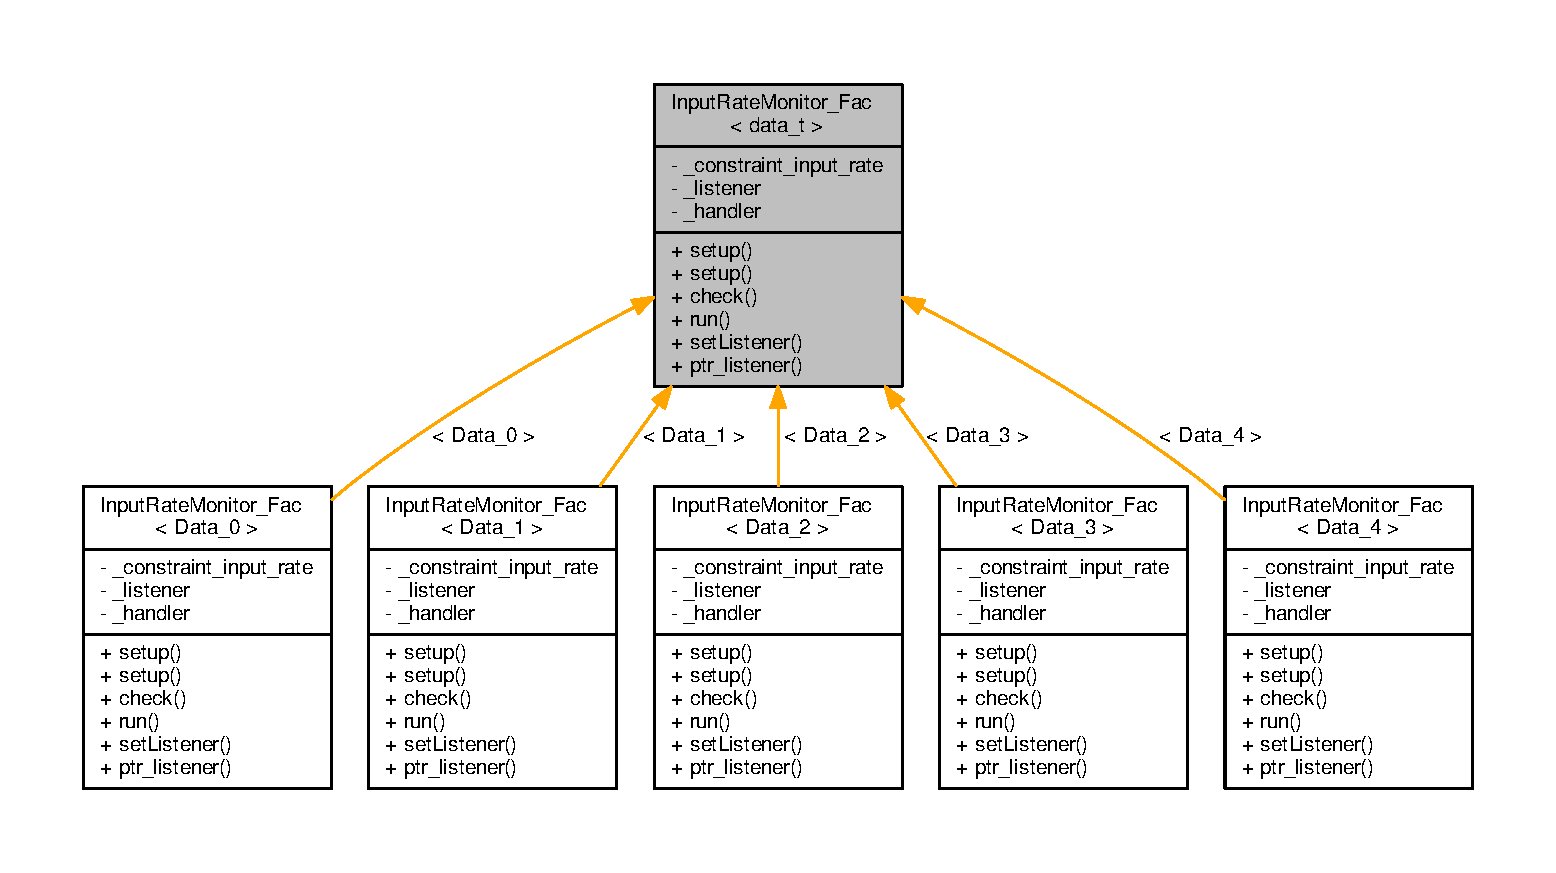
\includegraphics[width=350pt]{classInputRateMonitor__Fac__inherit__graph}
\end{center}
\end{figure}


Input\+Rate\+Monitor\+\_\+\+Fac$<$ data\+\_\+t $>$에 대한 협력 다이어그램\+:\nopagebreak
\begin{figure}[H]
\begin{center}
\leavevmode
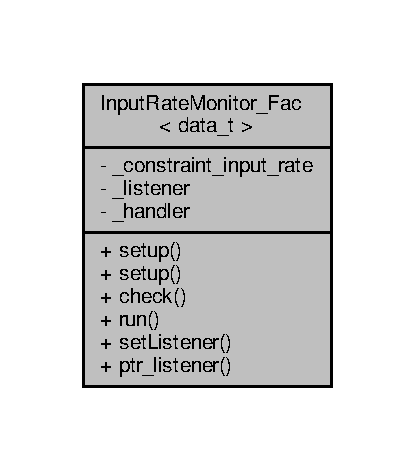
\includegraphics[width=199pt]{classInputRateMonitor__Fac__coll__graph}
\end{center}
\end{figure}
\subsection*{Public 멤버 함수}
\begin{DoxyCompactItemize}
\item 
void \hyperlink{classInputRateMonitor__Fac_a86fbd0921196702c3be28f817a3a0f97}{setup} (int input\+\_\+rate, void($\ast$\hyperlink{sample__main_8cpp_a57c221f281c346c72b89c10137fea994}{input\+\_\+rate\+\_\+handler})())
\item 
void \hyperlink{classInputRateMonitor__Fac_afced13486e1a312384898c7754063ff9}{setup} (int input\+\_\+rate, void($\ast$\hyperlink{sample__main_8cpp_a57c221f281c346c72b89c10137fea994}{input\+\_\+rate\+\_\+handler})(), void $\ast$user\+\_\+memory)
\item 
void \hyperlink{classInputRateMonitor__Fac_ae65b1007330c762d4df9e3b2751feed8}{check} ()
\item 
void \hyperlink{classInputRateMonitor__Fac_acf625ccd37afd9ad5c5728cc2c6873ce}{run} ()
\item 
void \hyperlink{classInputRateMonitor__Fac_ac5cd52f4b0a79964d61b93c30812912a}{set\+Listener} (\hyperlink{classSplashDataReaderListener}{Splash\+Data\+Reader\+Listener}$<$ data\+\_\+t $>$ $\ast$input\+\_\+rate\+\_\+listener)
\item 
\hyperlink{classSplashDataReaderListener}{Splash\+Data\+Reader\+Listener}$<$ data\+\_\+t $>$ $\ast$ \hyperlink{classInputRateMonitor__Fac_a1e515bd1ac53e333e6c2c1f34741d348}{ptr\+\_\+listener} ()
\end{DoxyCompactItemize}
\subsection*{Private 속성}
\begin{DoxyCompactItemize}
\item 
int \hyperlink{classInputRateMonitor__Fac_a9d144656510782c1ff3d34714b5fff0d}{\+\_\+constraint\+\_\+input\+\_\+rate} = -\/1
\item 
\hyperlink{classSplashDataReaderListener}{Splash\+Data\+Reader\+Listener}$<$ data\+\_\+t $>$ $\ast$ \hyperlink{classInputRateMonitor__Fac_a9dd55c51ebb699228894bfae73ba61c7}{\+\_\+listener}
\item 
void($\ast$ \hyperlink{classInputRateMonitor__Fac_af4e49691b122c46ce77d50ed6f34c477}{\+\_\+handler} )()
\end{DoxyCompactItemize}


\subsection{상세한 설명}
\subsubsection*{template$<$typename data\+\_\+t$>$\\*
class Input\+Rate\+Monitor\+\_\+\+Fac$<$ data\+\_\+t $>$}



Factory.\+cpp 파일의 312 번째 라인에서 정의되었습니다.



\subsection{멤버 함수 문서화}
\index{Input\+Rate\+Monitor\+\_\+\+Fac@{Input\+Rate\+Monitor\+\_\+\+Fac}!check@{check}}
\index{check@{check}!Input\+Rate\+Monitor\+\_\+\+Fac@{Input\+Rate\+Monitor\+\_\+\+Fac}}
\subsubsection[{\texorpdfstring{check()}{check()}}]{\setlength{\rightskip}{0pt plus 5cm}template$<$typename data\+\_\+t $>$ void {\bf Input\+Rate\+Monitor\+\_\+\+Fac}$<$ data\+\_\+t $>$\+::check (
\begin{DoxyParamCaption}
{}
\end{DoxyParamCaption}
)}\hypertarget{classInputRateMonitor__Fac_ae65b1007330c762d4df9e3b2751feed8}{}\label{classInputRateMonitor__Fac_ae65b1007330c762d4df9e3b2751feed8}


Factory.\+cpp 파일의 343 번째 라인에서 정의되었습니다.



다음을 참조함 \+:  Deadline\+Monitor\+\_\+\+Fac\+::\+\_\+handler, input\+\_\+rate\+\_\+handler().



이 함수 내부에서 호출하는 함수들에 대한 그래프입니다.\+:\nopagebreak
\begin{figure}[H]
\begin{center}
\leavevmode
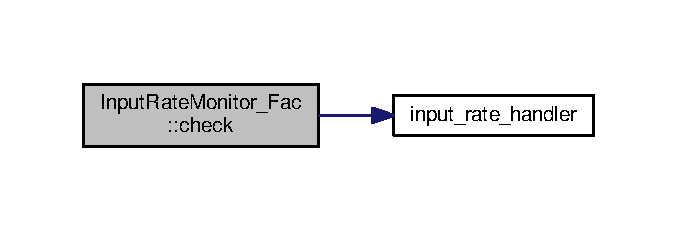
\includegraphics[width=325pt]{classInputRateMonitor__Fac_ae65b1007330c762d4df9e3b2751feed8_cgraph}
\end{center}
\end{figure}


\index{Input\+Rate\+Monitor\+\_\+\+Fac@{Input\+Rate\+Monitor\+\_\+\+Fac}!ptr\+\_\+listener@{ptr\+\_\+listener}}
\index{ptr\+\_\+listener@{ptr\+\_\+listener}!Input\+Rate\+Monitor\+\_\+\+Fac@{Input\+Rate\+Monitor\+\_\+\+Fac}}
\subsubsection[{\texorpdfstring{ptr\+\_\+listener()}{ptr_listener()}}]{\setlength{\rightskip}{0pt plus 5cm}template$<$typename data\+\_\+t $>$ {\bf Splash\+Data\+Reader\+Listener}$<$ data\+\_\+t $>$ $\ast$ {\bf Input\+Rate\+Monitor\+\_\+\+Fac}$<$ data\+\_\+t $>$\+::ptr\+\_\+listener (
\begin{DoxyParamCaption}
{}
\end{DoxyParamCaption}
)}\hypertarget{classInputRateMonitor__Fac_a1e515bd1ac53e333e6c2c1f34741d348}{}\label{classInputRateMonitor__Fac_a1e515bd1ac53e333e6c2c1f34741d348}


Factory.\+cpp 파일의 371 번째 라인에서 정의되었습니다.



다음에 의해서 참조됨 \+:  Input\+Data\+Port\+\_\+\+Fac$<$ Data\+\_\+0, Data\+\_\+1, Data\+\_\+2, Data\+\_\+3, Data\+\_\+4, Data\+\_\+5, Data\+\_\+6, Data\+\_\+7, Data\+\_\+8, Data\+\_\+9 $>$\+::attach().



이 함수를 호출하는 함수들에 대한 그래프입니다.\+:\nopagebreak
\begin{figure}[H]
\begin{center}
\leavevmode
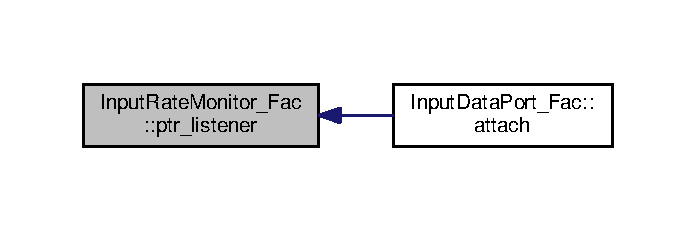
\includegraphics[width=334pt]{classInputRateMonitor__Fac_a1e515bd1ac53e333e6c2c1f34741d348_icgraph}
\end{center}
\end{figure}


\index{Input\+Rate\+Monitor\+\_\+\+Fac@{Input\+Rate\+Monitor\+\_\+\+Fac}!run@{run}}
\index{run@{run}!Input\+Rate\+Monitor\+\_\+\+Fac@{Input\+Rate\+Monitor\+\_\+\+Fac}}
\subsubsection[{\texorpdfstring{run()}{run()}}]{\setlength{\rightskip}{0pt plus 5cm}template$<$typename data\+\_\+t $>$ void {\bf Input\+Rate\+Monitor\+\_\+\+Fac}$<$ data\+\_\+t $>$\+::run (
\begin{DoxyParamCaption}
{}
\end{DoxyParamCaption}
)}\hypertarget{classInputRateMonitor__Fac_acf625ccd37afd9ad5c5728cc2c6873ce}{}\label{classInputRateMonitor__Fac_acf625ccd37afd9ad5c5728cc2c6873ce}


Factory.\+cpp 파일의 360 번째 라인에서 정의되었습니다.



다음에 의해서 참조됨 \+:  Input\+Data\+Port\+\_\+\+Fac$<$ Data\+\_\+0, Data\+\_\+1, Data\+\_\+2, Data\+\_\+3, Data\+\_\+4, Data\+\_\+5, Data\+\_\+6, Data\+\_\+7, Data\+\_\+8, Data\+\_\+9 $>$\+::initialize().



이 함수를 호출하는 함수들에 대한 그래프입니다.\+:\nopagebreak
\begin{figure}[H]
\begin{center}
\leavevmode
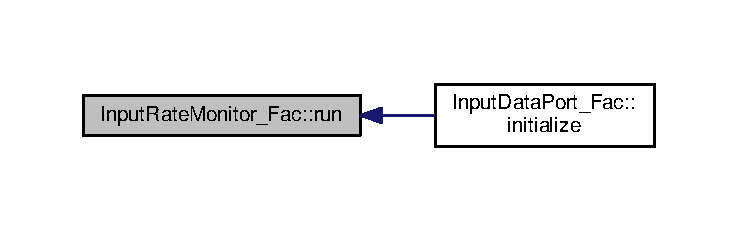
\includegraphics[width=350pt]{classInputRateMonitor__Fac_acf625ccd37afd9ad5c5728cc2c6873ce_icgraph}
\end{center}
\end{figure}


\index{Input\+Rate\+Monitor\+\_\+\+Fac@{Input\+Rate\+Monitor\+\_\+\+Fac}!set\+Listener@{set\+Listener}}
\index{set\+Listener@{set\+Listener}!Input\+Rate\+Monitor\+\_\+\+Fac@{Input\+Rate\+Monitor\+\_\+\+Fac}}
\subsubsection[{\texorpdfstring{set\+Listener(\+Splash\+Data\+Reader\+Listener$<$ data\+\_\+t $>$ $\ast$input\+\_\+rate\+\_\+listener)}{setListener(SplashDataReaderListener< data_t > *input_rate_listener)}}]{\setlength{\rightskip}{0pt plus 5cm}template$<$typename data\+\_\+t$>$ void {\bf Input\+Rate\+Monitor\+\_\+\+Fac}$<$ data\+\_\+t $>$\+::set\+Listener (
\begin{DoxyParamCaption}
\item[{{\bf Splash\+Data\+Reader\+Listener}$<$ data\+\_\+t $>$ $\ast$}]{input\+\_\+rate\+\_\+listener}
\end{DoxyParamCaption}
)}\hypertarget{classInputRateMonitor__Fac_ac5cd52f4b0a79964d61b93c30812912a}{}\label{classInputRateMonitor__Fac_ac5cd52f4b0a79964d61b93c30812912a}


Factory.\+cpp 파일의 366 번째 라인에서 정의되었습니다.



다음에 의해서 참조됨 \+:  Input\+Data\+Port\+\_\+\+Fac$<$ Data\+\_\+0, Data\+\_\+1, Data\+\_\+2, Data\+\_\+3, Data\+\_\+4, Data\+\_\+5, Data\+\_\+6, Data\+\_\+7, Data\+\_\+8, Data\+\_\+9 $>$\+::attach().



이 함수를 호출하는 함수들에 대한 그래프입니다.\+:\nopagebreak
\begin{figure}[H]
\begin{center}
\leavevmode
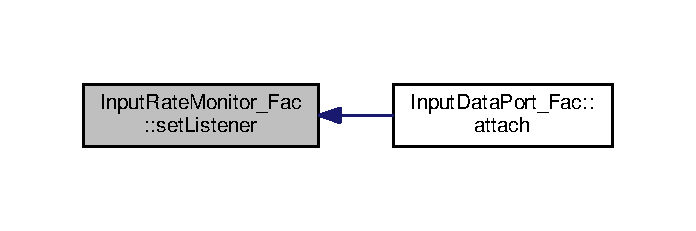
\includegraphics[width=334pt]{classInputRateMonitor__Fac_ac5cd52f4b0a79964d61b93c30812912a_icgraph}
\end{center}
\end{figure}


\index{Input\+Rate\+Monitor\+\_\+\+Fac@{Input\+Rate\+Monitor\+\_\+\+Fac}!setup@{setup}}
\index{setup@{setup}!Input\+Rate\+Monitor\+\_\+\+Fac@{Input\+Rate\+Monitor\+\_\+\+Fac}}
\subsubsection[{\texorpdfstring{setup(int input\+\_\+rate, void($\ast$input\+\_\+rate\+\_\+handler)())}{setup(int input_rate, void(*input_rate_handler)())}}]{\setlength{\rightskip}{0pt plus 5cm}template$<$typename data\+\_\+t $>$ void {\bf Input\+Rate\+Monitor\+\_\+\+Fac}$<$ data\+\_\+t $>$\+::setup (
\begin{DoxyParamCaption}
\item[{int}]{input\+\_\+rate, }
\item[{void($\ast$)()}]{input\+\_\+rate\+\_\+handler}
\end{DoxyParamCaption}
)}\hypertarget{classInputRateMonitor__Fac_a86fbd0921196702c3be28f817a3a0f97}{}\label{classInputRateMonitor__Fac_a86fbd0921196702c3be28f817a3a0f97}


Factory.\+cpp 파일의 331 번째 라인에서 정의되었습니다.



다음을 참조함 \+:  Deadline\+Monitor\+\_\+\+Fac\+::\+\_\+handler, input\+\_\+rate\+\_\+handler().



다음에 의해서 참조됨 \+:  Input\+Data\+Port\+\_\+\+Fac$<$ Data\+\_\+0, Data\+\_\+1, Data\+\_\+2, Data\+\_\+3, Data\+\_\+4, Data\+\_\+5, Data\+\_\+6, Data\+\_\+7, Data\+\_\+8, Data\+\_\+9 $>$\+::initialize().



이 함수 내부에서 호출하는 함수들에 대한 그래프입니다.\+:\nopagebreak
\begin{figure}[H]
\begin{center}
\leavevmode
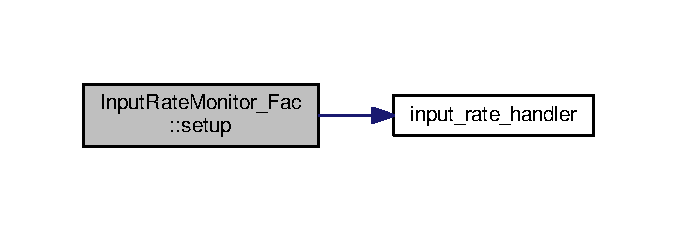
\includegraphics[width=325pt]{classInputRateMonitor__Fac_a86fbd0921196702c3be28f817a3a0f97_cgraph}
\end{center}
\end{figure}




이 함수를 호출하는 함수들에 대한 그래프입니다.\+:\nopagebreak
\begin{figure}[H]
\begin{center}
\leavevmode
\includegraphics[width=334pt]{classInputRateMonitor__Fac_a86fbd0921196702c3be28f817a3a0f97_icgraph}
\end{center}
\end{figure}


\index{Input\+Rate\+Monitor\+\_\+\+Fac@{Input\+Rate\+Monitor\+\_\+\+Fac}!setup@{setup}}
\index{setup@{setup}!Input\+Rate\+Monitor\+\_\+\+Fac@{Input\+Rate\+Monitor\+\_\+\+Fac}}
\subsubsection[{\texorpdfstring{setup(int input\+\_\+rate, void($\ast$input\+\_\+rate\+\_\+handler)(), void $\ast$user\+\_\+memory)}{setup(int input_rate, void(*input_rate_handler)(), void *user_memory)}}]{\setlength{\rightskip}{0pt plus 5cm}template$<$typename data\+\_\+t $>$ void {\bf Input\+Rate\+Monitor\+\_\+\+Fac}$<$ data\+\_\+t $>$\+::setup (
\begin{DoxyParamCaption}
\item[{int}]{input\+\_\+rate, }
\item[{void($\ast$)()}]{input\+\_\+rate\+\_\+handler, }
\item[{void $\ast$}]{user\+\_\+memory}
\end{DoxyParamCaption}
)}\hypertarget{classInputRateMonitor__Fac_afced13486e1a312384898c7754063ff9}{}\label{classInputRateMonitor__Fac_afced13486e1a312384898c7754063ff9}


Factory.\+cpp 파일의 337 번째 라인에서 정의되었습니다.



다음을 참조함 \+:  Deadline\+Monitor\+\_\+\+Fac\+::\+\_\+handler, input\+\_\+rate\+\_\+handler().



이 함수 내부에서 호출하는 함수들에 대한 그래프입니다.\+:\nopagebreak
\begin{figure}[H]
\begin{center}
\leavevmode
\includegraphics[width=325pt]{classInputRateMonitor__Fac_afced13486e1a312384898c7754063ff9_cgraph}
\end{center}
\end{figure}




\subsection{멤버 데이타 문서화}
\index{Input\+Rate\+Monitor\+\_\+\+Fac@{Input\+Rate\+Monitor\+\_\+\+Fac}!\+\_\+constraint\+\_\+input\+\_\+rate@{\+\_\+constraint\+\_\+input\+\_\+rate}}
\index{\+\_\+constraint\+\_\+input\+\_\+rate@{\+\_\+constraint\+\_\+input\+\_\+rate}!Input\+Rate\+Monitor\+\_\+\+Fac@{Input\+Rate\+Monitor\+\_\+\+Fac}}
\subsubsection[{\texorpdfstring{\+\_\+constraint\+\_\+input\+\_\+rate}{_constraint_input_rate}}]{\setlength{\rightskip}{0pt plus 5cm}template$<$typename data\+\_\+t$>$ int {\bf Input\+Rate\+Monitor\+\_\+\+Fac}$<$ data\+\_\+t $>$\+::\+\_\+constraint\+\_\+input\+\_\+rate = -\/1\hspace{0.3cm}{\ttfamily [private]}}\hypertarget{classInputRateMonitor__Fac_a9d144656510782c1ff3d34714b5fff0d}{}\label{classInputRateMonitor__Fac_a9d144656510782c1ff3d34714b5fff0d}


Factory.\+cpp 파일의 324 번째 라인에서 정의되었습니다.

\index{Input\+Rate\+Monitor\+\_\+\+Fac@{Input\+Rate\+Monitor\+\_\+\+Fac}!\+\_\+handler@{\+\_\+handler}}
\index{\+\_\+handler@{\+\_\+handler}!Input\+Rate\+Monitor\+\_\+\+Fac@{Input\+Rate\+Monitor\+\_\+\+Fac}}
\subsubsection[{\texorpdfstring{\+\_\+handler}{_handler}}]{\setlength{\rightskip}{0pt plus 5cm}template$<$typename data\+\_\+t$>$ void($\ast$ {\bf Input\+Rate\+Monitor\+\_\+\+Fac}$<$ data\+\_\+t $>$\+::\+\_\+handler) ()\hspace{0.3cm}{\ttfamily [private]}}\hypertarget{classInputRateMonitor__Fac_af4e49691b122c46ce77d50ed6f34c477}{}\label{classInputRateMonitor__Fac_af4e49691b122c46ce77d50ed6f34c477}


Factory.\+cpp 파일의 326 번째 라인에서 정의되었습니다.

\index{Input\+Rate\+Monitor\+\_\+\+Fac@{Input\+Rate\+Monitor\+\_\+\+Fac}!\+\_\+listener@{\+\_\+listener}}
\index{\+\_\+listener@{\+\_\+listener}!Input\+Rate\+Monitor\+\_\+\+Fac@{Input\+Rate\+Monitor\+\_\+\+Fac}}
\subsubsection[{\texorpdfstring{\+\_\+listener}{_listener}}]{\setlength{\rightskip}{0pt plus 5cm}template$<$typename data\+\_\+t$>$ {\bf Splash\+Data\+Reader\+Listener}$<$data\+\_\+t$>$$\ast$ {\bf Input\+Rate\+Monitor\+\_\+\+Fac}$<$ data\+\_\+t $>$\+::\+\_\+listener\hspace{0.3cm}{\ttfamily [private]}}\hypertarget{classInputRateMonitor__Fac_a9dd55c51ebb699228894bfae73ba61c7}{}\label{classInputRateMonitor__Fac_a9dd55c51ebb699228894bfae73ba61c7}


Factory.\+cpp 파일의 325 번째 라인에서 정의되었습니다.



이 클래스에 대한 문서화 페이지는 다음의 파일로부터 생성되었습니다.\+:\begin{DoxyCompactItemize}
\item 
src/\hyperlink{Factory_8cpp}{Factory.\+cpp}\end{DoxyCompactItemize}

\hypertarget{classInputRateMonitor__PB}{}\section{Input\+Rate\+Monitor\+\_\+\+PB$<$ data\+\_\+t $>$}
\label{classInputRateMonitor__PB}\index{Input\+Rate\+Monitor\+\_\+\+P\+B$<$ data\+\_\+t $>$@{Input\+Rate\+Monitor\+\_\+\+P\+B$<$ data\+\_\+t $>$}}


detect input rate constriant violation  




Input\+Rate\+Monitor\+\_\+\+PB$<$ data\+\_\+t $>$에 대한 상속 다이어그램 \+: \nopagebreak
\begin{figure}[H]
\begin{center}
\leavevmode
\includegraphics[width=350pt]{classInputRateMonitor__PB__inherit__graph}
\end{center}
\end{figure}


Input\+Rate\+Monitor\+\_\+\+PB$<$ data\+\_\+t $>$에 대한 협력 다이어그램\+:\nopagebreak
\begin{figure}[H]
\begin{center}
\leavevmode
\includegraphics[width=199pt]{classInputRateMonitor__PB__coll__graph}
\end{center}
\end{figure}
\subsection*{Public 멤버 함수}
\begin{DoxyCompactItemize}
\item 
void \hyperlink{classInputRateMonitor__PB_ab37591b8f43422bacbaab7ce4b8ba7e7}{setup} (int input\+\_\+rate, void($\ast$\hyperlink{sample__main_8cpp_a57c221f281c346c72b89c10137fea994}{input\+\_\+rate\+\_\+handler})())
\item 
void \hyperlink{classInputRateMonitor__PB_aea065d055e3cb4ec2221a7c95e12a98f}{setup} (int input\+\_\+rate, void($\ast$\hyperlink{sample__main_8cpp_a57c221f281c346c72b89c10137fea994}{input\+\_\+rate\+\_\+handler})(), void $\ast$user\+\_\+memory)
\item 
void \hyperlink{classInputRateMonitor__PB_a7f912ff558127c5a951c186c0c9ad2ee}{check} ()
\item 
void \hyperlink{classInputRateMonitor__PB_a078f5a23b3fff392b7f50a9d376ded0b}{run} ()
\item 
void \hyperlink{classInputRateMonitor__PB_a3e62dd99866737bf5f7be82c16433940}{set\+Listener} (\hyperlink{classSplashDataReaderListener}{Splash\+Data\+Reader\+Listener}$<$ data\+\_\+t $>$ $\ast$input\+\_\+rate\+\_\+listener)
\item 
\hyperlink{classSplashDataReaderListener}{Splash\+Data\+Reader\+Listener}$<$ data\+\_\+t $>$ $\ast$ \hyperlink{classInputRateMonitor__PB_a7fd5f7e9be9ab5f62f2122ed5f43100a}{ptr\+\_\+listener} ()
\end{DoxyCompactItemize}
\subsection*{Private 속성}
\begin{DoxyCompactItemize}
\item 
int \hyperlink{classInputRateMonitor__PB_a1294a164e2a5c966599d0802cf4fed24}{\+\_\+constraint\+\_\+input\+\_\+rate} = -\/1
\item 
\hyperlink{classSplashDataReaderListener}{Splash\+Data\+Reader\+Listener}$<$ data\+\_\+t $>$ $\ast$ \hyperlink{classInputRateMonitor__PB_a5d9bb568b165fe454daced915ecc6c7e}{\+\_\+listener}
\item 
void($\ast$ \hyperlink{classInputRateMonitor__PB_ab8e00bdce1779070b9587f477ee281a7}{\+\_\+handler} )()
\end{DoxyCompactItemize}


\subsection{상세한 설명}
\subsubsection*{template$<$typename data\+\_\+t$>$\\*
class Input\+Rate\+Monitor\+\_\+\+P\+B$<$ data\+\_\+t $>$}

detect input rate constriant violation 

\begin{DoxyAuthor}{작성자}
Beomjoon Yang 
\end{DoxyAuthor}
\begin{DoxyDate}{날짜}
2018-\/10-\/26 
\end{DoxyDate}
\begin{DoxyVersion}{버전}
0.\+0.\+1 
\end{DoxyVersion}


Processing\+\_\+block.\+cpp 파일의 546 번째 라인에서 정의되었습니다.



\subsection{멤버 함수 문서화}
\index{Input\+Rate\+Monitor\+\_\+\+PB@{Input\+Rate\+Monitor\+\_\+\+PB}!check@{check}}
\index{check@{check}!Input\+Rate\+Monitor\+\_\+\+PB@{Input\+Rate\+Monitor\+\_\+\+PB}}
\subsubsection[{\texorpdfstring{check()}{check()}}]{\setlength{\rightskip}{0pt plus 5cm}template$<$typename data\+\_\+t $>$ void {\bf Input\+Rate\+Monitor\+\_\+\+PB}$<$ data\+\_\+t $>$\+::check (
\begin{DoxyParamCaption}
{}
\end{DoxyParamCaption}
)}\hypertarget{classInputRateMonitor__PB_a7f912ff558127c5a951c186c0c9ad2ee}{}\label{classInputRateMonitor__PB_a7f912ff558127c5a951c186c0c9ad2ee}


Processing\+\_\+block.\+cpp 파일의 577 번째 라인에서 정의되었습니다.



다음을 참조함 \+:  input\+\_\+rate\+\_\+handler().



이 함수 내부에서 호출하는 함수들에 대한 그래프입니다.\+:\nopagebreak
\begin{figure}[H]
\begin{center}
\leavevmode
\includegraphics[width=322pt]{classInputRateMonitor__PB_a7f912ff558127c5a951c186c0c9ad2ee_cgraph}
\end{center}
\end{figure}


\index{Input\+Rate\+Monitor\+\_\+\+PB@{Input\+Rate\+Monitor\+\_\+\+PB}!ptr\+\_\+listener@{ptr\+\_\+listener}}
\index{ptr\+\_\+listener@{ptr\+\_\+listener}!Input\+Rate\+Monitor\+\_\+\+PB@{Input\+Rate\+Monitor\+\_\+\+PB}}
\subsubsection[{\texorpdfstring{ptr\+\_\+listener()}{ptr_listener()}}]{\setlength{\rightskip}{0pt plus 5cm}template$<$typename data\+\_\+t $>$ {\bf Splash\+Data\+Reader\+Listener}$<$ data\+\_\+t $>$ $\ast$ {\bf Input\+Rate\+Monitor\+\_\+\+PB}$<$ data\+\_\+t $>$\+::ptr\+\_\+listener (
\begin{DoxyParamCaption}
{}
\end{DoxyParamCaption}
)}\hypertarget{classInputRateMonitor__PB_a7fd5f7e9be9ab5f62f2122ed5f43100a}{}\label{classInputRateMonitor__PB_a7fd5f7e9be9ab5f62f2122ed5f43100a}


Processing\+\_\+block.\+cpp 파일의 605 번째 라인에서 정의되었습니다.



다음에 의해서 참조됨 \+:  Input\+Data\+Port\+\_\+\+P\+B$<$ Data\+\_\+0, Data\+\_\+1, Data\+\_\+2, Data\+\_\+3, Data\+\_\+4, Data\+\_\+5, Data\+\_\+6, Data\+\_\+7, Data\+\_\+8, Data\+\_\+9 $>$\+::check\+Freshness().



이 함수를 호출하는 함수들에 대한 그래프입니다.\+:\nopagebreak
\begin{figure}[H]
\begin{center}
\leavevmode
\includegraphics[width=350pt]{classInputRateMonitor__PB_a7fd5f7e9be9ab5f62f2122ed5f43100a_icgraph}
\end{center}
\end{figure}


\index{Input\+Rate\+Monitor\+\_\+\+PB@{Input\+Rate\+Monitor\+\_\+\+PB}!run@{run}}
\index{run@{run}!Input\+Rate\+Monitor\+\_\+\+PB@{Input\+Rate\+Monitor\+\_\+\+PB}}
\subsubsection[{\texorpdfstring{run()}{run()}}]{\setlength{\rightskip}{0pt plus 5cm}template$<$typename data\+\_\+t $>$ void {\bf Input\+Rate\+Monitor\+\_\+\+PB}$<$ data\+\_\+t $>$\+::run (
\begin{DoxyParamCaption}
{}
\end{DoxyParamCaption}
)}\hypertarget{classInputRateMonitor__PB_a078f5a23b3fff392b7f50a9d376ded0b}{}\label{classInputRateMonitor__PB_a078f5a23b3fff392b7f50a9d376ded0b}


Processing\+\_\+block.\+cpp 파일의 594 번째 라인에서 정의되었습니다.



다음에 의해서 참조됨 \+:  Input\+Data\+Port\+\_\+\+P\+B$<$ Data\+\_\+0, Data\+\_\+1, Data\+\_\+2, Data\+\_\+3, Data\+\_\+4, Data\+\_\+5, Data\+\_\+6, Data\+\_\+7, Data\+\_\+8, Data\+\_\+9 $>$\+::initialize().



이 함수를 호출하는 함수들에 대한 그래프입니다.\+:\nopagebreak
\begin{figure}[H]
\begin{center}
\leavevmode
\includegraphics[width=350pt]{classInputRateMonitor__PB_a078f5a23b3fff392b7f50a9d376ded0b_icgraph}
\end{center}
\end{figure}


\index{Input\+Rate\+Monitor\+\_\+\+PB@{Input\+Rate\+Monitor\+\_\+\+PB}!set\+Listener@{set\+Listener}}
\index{set\+Listener@{set\+Listener}!Input\+Rate\+Monitor\+\_\+\+PB@{Input\+Rate\+Monitor\+\_\+\+PB}}
\subsubsection[{\texorpdfstring{set\+Listener(\+Splash\+Data\+Reader\+Listener$<$ data\+\_\+t $>$ $\ast$input\+\_\+rate\+\_\+listener)}{setListener(SplashDataReaderListener< data_t > *input_rate_listener)}}]{\setlength{\rightskip}{0pt plus 5cm}template$<$typename data\+\_\+t$>$ void {\bf Input\+Rate\+Monitor\+\_\+\+PB}$<$ data\+\_\+t $>$\+::set\+Listener (
\begin{DoxyParamCaption}
\item[{{\bf Splash\+Data\+Reader\+Listener}$<$ data\+\_\+t $>$ $\ast$}]{input\+\_\+rate\+\_\+listener}
\end{DoxyParamCaption}
)}\hypertarget{classInputRateMonitor__PB_a3e62dd99866737bf5f7be82c16433940}{}\label{classInputRateMonitor__PB_a3e62dd99866737bf5f7be82c16433940}


Processing\+\_\+block.\+cpp 파일의 600 번째 라인에서 정의되었습니다.



다음에 의해서 참조됨 \+:  Input\+Data\+Port\+\_\+\+P\+B$<$ Data\+\_\+0, Data\+\_\+1, Data\+\_\+2, Data\+\_\+3, Data\+\_\+4, Data\+\_\+5, Data\+\_\+6, Data\+\_\+7, Data\+\_\+8, Data\+\_\+9 $>$\+::check\+Freshness().



이 함수를 호출하는 함수들에 대한 그래프입니다.\+:\nopagebreak
\begin{figure}[H]
\begin{center}
\leavevmode
\includegraphics[width=350pt]{classInputRateMonitor__PB_a3e62dd99866737bf5f7be82c16433940_icgraph}
\end{center}
\end{figure}


\index{Input\+Rate\+Monitor\+\_\+\+PB@{Input\+Rate\+Monitor\+\_\+\+PB}!setup@{setup}}
\index{setup@{setup}!Input\+Rate\+Monitor\+\_\+\+PB@{Input\+Rate\+Monitor\+\_\+\+PB}}
\subsubsection[{\texorpdfstring{setup(int input\+\_\+rate, void($\ast$input\+\_\+rate\+\_\+handler)())}{setup(int input_rate, void(*input_rate_handler)())}}]{\setlength{\rightskip}{0pt plus 5cm}template$<$typename data\+\_\+t $>$ void {\bf Input\+Rate\+Monitor\+\_\+\+PB}$<$ data\+\_\+t $>$\+::setup (
\begin{DoxyParamCaption}
\item[{int}]{input\+\_\+rate, }
\item[{void($\ast$)()}]{input\+\_\+rate\+\_\+handler}
\end{DoxyParamCaption}
)}\hypertarget{classInputRateMonitor__PB_ab37591b8f43422bacbaab7ce4b8ba7e7}{}\label{classInputRateMonitor__PB_ab37591b8f43422bacbaab7ce4b8ba7e7}


Processing\+\_\+block.\+cpp 파일의 565 번째 라인에서 정의되었습니다.



다음을 참조함 \+:  input\+\_\+rate\+\_\+handler().



다음에 의해서 참조됨 \+:  Input\+Data\+Port\+\_\+\+P\+B$<$ Data\+\_\+0, Data\+\_\+1, Data\+\_\+2, Data\+\_\+3, Data\+\_\+4, Data\+\_\+5, Data\+\_\+6, Data\+\_\+7, Data\+\_\+8, Data\+\_\+9 $>$\+::initialize().



이 함수 내부에서 호출하는 함수들에 대한 그래프입니다.\+:\nopagebreak
\begin{figure}[H]
\begin{center}
\leavevmode
\includegraphics[width=322pt]{classInputRateMonitor__PB_ab37591b8f43422bacbaab7ce4b8ba7e7_cgraph}
\end{center}
\end{figure}




이 함수를 호출하는 함수들에 대한 그래프입니다.\+:\nopagebreak
\begin{figure}[H]
\begin{center}
\leavevmode
\includegraphics[width=350pt]{classInputRateMonitor__PB_ab37591b8f43422bacbaab7ce4b8ba7e7_icgraph}
\end{center}
\end{figure}


\index{Input\+Rate\+Monitor\+\_\+\+PB@{Input\+Rate\+Monitor\+\_\+\+PB}!setup@{setup}}
\index{setup@{setup}!Input\+Rate\+Monitor\+\_\+\+PB@{Input\+Rate\+Monitor\+\_\+\+PB}}
\subsubsection[{\texorpdfstring{setup(int input\+\_\+rate, void($\ast$input\+\_\+rate\+\_\+handler)(), void $\ast$user\+\_\+memory)}{setup(int input_rate, void(*input_rate_handler)(), void *user_memory)}}]{\setlength{\rightskip}{0pt plus 5cm}template$<$typename data\+\_\+t $>$ void {\bf Input\+Rate\+Monitor\+\_\+\+PB}$<$ data\+\_\+t $>$\+::setup (
\begin{DoxyParamCaption}
\item[{int}]{input\+\_\+rate, }
\item[{void($\ast$)()}]{input\+\_\+rate\+\_\+handler, }
\item[{void $\ast$}]{user\+\_\+memory}
\end{DoxyParamCaption}
)}\hypertarget{classInputRateMonitor__PB_aea065d055e3cb4ec2221a7c95e12a98f}{}\label{classInputRateMonitor__PB_aea065d055e3cb4ec2221a7c95e12a98f}


Processing\+\_\+block.\+cpp 파일의 571 번째 라인에서 정의되었습니다.



다음을 참조함 \+:  input\+\_\+rate\+\_\+handler().



이 함수 내부에서 호출하는 함수들에 대한 그래프입니다.\+:\nopagebreak
\begin{figure}[H]
\begin{center}
\leavevmode
\includegraphics[width=322pt]{classInputRateMonitor__PB_aea065d055e3cb4ec2221a7c95e12a98f_cgraph}
\end{center}
\end{figure}




\subsection{멤버 데이타 문서화}
\index{Input\+Rate\+Monitor\+\_\+\+PB@{Input\+Rate\+Monitor\+\_\+\+PB}!\+\_\+constraint\+\_\+input\+\_\+rate@{\+\_\+constraint\+\_\+input\+\_\+rate}}
\index{\+\_\+constraint\+\_\+input\+\_\+rate@{\+\_\+constraint\+\_\+input\+\_\+rate}!Input\+Rate\+Monitor\+\_\+\+PB@{Input\+Rate\+Monitor\+\_\+\+PB}}
\subsubsection[{\texorpdfstring{\+\_\+constraint\+\_\+input\+\_\+rate}{_constraint_input_rate}}]{\setlength{\rightskip}{0pt plus 5cm}template$<$typename data\+\_\+t$>$ int {\bf Input\+Rate\+Monitor\+\_\+\+PB}$<$ data\+\_\+t $>$\+::\+\_\+constraint\+\_\+input\+\_\+rate = -\/1\hspace{0.3cm}{\ttfamily [private]}}\hypertarget{classInputRateMonitor__PB_a1294a164e2a5c966599d0802cf4fed24}{}\label{classInputRateMonitor__PB_a1294a164e2a5c966599d0802cf4fed24}


Processing\+\_\+block.\+cpp 파일의 558 번째 라인에서 정의되었습니다.

\index{Input\+Rate\+Monitor\+\_\+\+PB@{Input\+Rate\+Monitor\+\_\+\+PB}!\+\_\+handler@{\+\_\+handler}}
\index{\+\_\+handler@{\+\_\+handler}!Input\+Rate\+Monitor\+\_\+\+PB@{Input\+Rate\+Monitor\+\_\+\+PB}}
\subsubsection[{\texorpdfstring{\+\_\+handler}{_handler}}]{\setlength{\rightskip}{0pt plus 5cm}template$<$typename data\+\_\+t$>$ void($\ast$ {\bf Input\+Rate\+Monitor\+\_\+\+PB}$<$ data\+\_\+t $>$\+::\+\_\+handler) ()\hspace{0.3cm}{\ttfamily [private]}}\hypertarget{classInputRateMonitor__PB_ab8e00bdce1779070b9587f477ee281a7}{}\label{classInputRateMonitor__PB_ab8e00bdce1779070b9587f477ee281a7}


Processing\+\_\+block.\+cpp 파일의 560 번째 라인에서 정의되었습니다.

\index{Input\+Rate\+Monitor\+\_\+\+PB@{Input\+Rate\+Monitor\+\_\+\+PB}!\+\_\+listener@{\+\_\+listener}}
\index{\+\_\+listener@{\+\_\+listener}!Input\+Rate\+Monitor\+\_\+\+PB@{Input\+Rate\+Monitor\+\_\+\+PB}}
\subsubsection[{\texorpdfstring{\+\_\+listener}{_listener}}]{\setlength{\rightskip}{0pt plus 5cm}template$<$typename data\+\_\+t$>$ {\bf Splash\+Data\+Reader\+Listener}$<$data\+\_\+t$>$$\ast$ {\bf Input\+Rate\+Monitor\+\_\+\+PB}$<$ data\+\_\+t $>$\+::\+\_\+listener\hspace{0.3cm}{\ttfamily [private]}}\hypertarget{classInputRateMonitor__PB_a5d9bb568b165fe454daced915ecc6c7e}{}\label{classInputRateMonitor__PB_a5d9bb568b165fe454daced915ecc6c7e}


Processing\+\_\+block.\+cpp 파일의 559 번째 라인에서 정의되었습니다.



이 클래스에 대한 문서화 페이지는 다음의 파일로부터 생성되었습니다.\+:\begin{DoxyCompactItemize}
\item 
src/\hyperlink{Processing__block_8cpp}{Processing\+\_\+block.\+cpp}\end{DoxyCompactItemize}

\hypertarget{classOutputDataPort}{}\section{Output\+Data\+Port$<$ Data\+\_\+0, Data\+\_\+1, Data\+\_\+2, Data\+\_\+3, Data\+\_\+4, Data\+\_\+5, Data\+\_\+6, Data\+\_\+7, Data\+\_\+8, Data\+\_\+9 $>$}
\label{classOutputDataPort}\index{Output\+Data\+Port$<$ Data\+\_\+0, Data\+\_\+1, Data\+\_\+2, Data\+\_\+3, Data\+\_\+4, Data\+\_\+5, Data\+\_\+6, Data\+\_\+7, Data\+\_\+8, Data\+\_\+9 $>$@{Output\+Data\+Port$<$ Data\+\_\+0, Data\+\_\+1, Data\+\_\+2, Data\+\_\+3, Data\+\_\+4, Data\+\_\+5, Data\+\_\+6, Data\+\_\+7, Data\+\_\+8, Data\+\_\+9 $>$}}


Output\+Data\+Port$<$ Data\+\_\+0, Data\+\_\+1, Data\+\_\+2, Data\+\_\+3, Data\+\_\+4, Data\+\_\+5, Data\+\_\+6, Data\+\_\+7, Data\+\_\+8, Data\+\_\+9 $>$에 대한 협력 다이어그램\+:\nopagebreak
\begin{figure}[H]
\begin{center}
\leavevmode
\includegraphics[width=229pt]{classOutputDataPort__coll__graph}
\end{center}
\end{figure}


\subsection{상세한 설명}
\subsubsection*{template$<$typename Data\+\_\+0, typename Data\+\_\+1, typename Data\+\_\+2, typename Data\+\_\+3, typename Data\+\_\+4, typename Data\+\_\+5, typename Data\+\_\+6, typename Data\+\_\+7, typename Data\+\_\+8, typename Data\+\_\+9$>$\\*
class Output\+Data\+Port$<$ Data\+\_\+0, Data\+\_\+1, Data\+\_\+2, Data\+\_\+3, Data\+\_\+4, Data\+\_\+5, Data\+\_\+6, Data\+\_\+7, Data\+\_\+8, Data\+\_\+9 $>$}



Base\+\_\+cell\+\_\+temp.\+cpp 파일의 19 번째 라인에서 정의되었습니다.



이 클래스에 대한 문서화 페이지는 다음의 파일로부터 생성되었습니다.\+:\begin{DoxyCompactItemize}
\item 
src/\hyperlink{Base__cell__temp_8cpp}{Base\+\_\+cell\+\_\+temp.\+cpp}\end{DoxyCompactItemize}

\hypertarget{classOutputDataPort__F}{}\section{Output\+Data\+Port\+\_\+F$<$ Data\+\_\+0, Data\+\_\+1, Data\+\_\+2, Data\+\_\+3, Data\+\_\+4, Data\+\_\+5, Data\+\_\+6, Data\+\_\+7, Data\+\_\+8, Data\+\_\+9 $>$}
\label{classOutputDataPort__F}\index{Output\+Data\+Port\+\_\+\+F$<$ Data\+\_\+0, Data\+\_\+1, Data\+\_\+2, Data\+\_\+3, Data\+\_\+4, Data\+\_\+5, Data\+\_\+6, Data\+\_\+7, Data\+\_\+8, Data\+\_\+9 $>$@{Output\+Data\+Port\+\_\+\+F$<$ Data\+\_\+0, Data\+\_\+1, Data\+\_\+2, Data\+\_\+3, Data\+\_\+4, Data\+\_\+5, Data\+\_\+6, Data\+\_\+7, Data\+\_\+8, Data\+\_\+9 $>$}}


Output\+Data\+Port\+\_\+F$<$ Data\+\_\+0, Data\+\_\+1, Data\+\_\+2, Data\+\_\+3, Data\+\_\+4, Data\+\_\+5, Data\+\_\+6, Data\+\_\+7, Data\+\_\+8, Data\+\_\+9 $>$에 대한 협력 다이어그램\+:\nopagebreak
\begin{figure}[H]
\begin{center}
\leavevmode
\includegraphics[width=229pt]{classOutputDataPort__F__coll__graph}
\end{center}
\end{figure}
\subsection*{Public 멤버 함수}
\begin{DoxyCompactItemize}
\item 
int \hyperlink{classOutputDataPort__F_a7a80d278d8aa04b8b884ab0f7753a528}{attach} (\hyperlink{classFusion__operator}{Fusion\+\_\+operator}$<$Data\+\_\+0, Data\+\_\+1, Data\+\_\+2, Data\+\_\+3, Data\+\_\+4, Data\+\_\+5, Data\+\_\+6, Data\+\_\+7, Data\+\_\+8, Data\+\_\+9 $>$ $\ast$, std\+::string)
\item 
void \hyperlink{classOutputDataPort__F_a08064705099380038f1a035f4bbdfd12}{initialize} (double rate)
\end{DoxyCompactItemize}
\subsection*{Public 속성}
\begin{DoxyCompactItemize}
\item 
dds\+::pub\+::\+Data\+Writer$<$ Data\+\_\+9 $>$ $\ast$ \hyperlink{classOutputDataPort__F_a269553e496d1229e4f88e6449a2bce8e}{O\+D\+P\+\_\+writer}
\end{DoxyCompactItemize}


\subsection{상세한 설명}
\subsubsection*{template$<$typename Data\+\_\+0, typename Data\+\_\+1, typename Data\+\_\+2, typename Data\+\_\+3, typename Data\+\_\+4, typename Data\+\_\+5, typename Data\+\_\+6, typename Data\+\_\+7, typename Data\+\_\+8, typename Data\+\_\+9$>$\\*
class Output\+Data\+Port\+\_\+\+F$<$ Data\+\_\+0, Data\+\_\+1, Data\+\_\+2, Data\+\_\+3, Data\+\_\+4, Data\+\_\+5, Data\+\_\+6, Data\+\_\+7, Data\+\_\+8, Data\+\_\+9 $>$}



Fusion\+\_\+operator.\+cpp 파일의 24 번째 라인에서 정의되었습니다.



\subsection{멤버 함수 문서화}
\index{Output\+Data\+Port\+\_\+F@{Output\+Data\+Port\+\_\+F}!attach@{attach}}
\index{attach@{attach}!Output\+Data\+Port\+\_\+F@{Output\+Data\+Port\+\_\+F}}
\subsubsection[{\texorpdfstring{attach(\+Fusion\+\_\+operator$<$\+Data\+\_\+0, Data\+\_\+1, Data\+\_\+2, Data\+\_\+3, Data\+\_\+4, Data\+\_\+5, Data\+\_\+6, Data\+\_\+7, Data\+\_\+8, Data\+\_\+9 $>$ $\ast$, std\+::string)}{attach(Fusion_operator<Data_0, Data_1, Data_2, Data_3, Data_4, Data_5, Data_6, Data_7, Data_8, Data_9 > *, std::string)}}]{\setlength{\rightskip}{0pt plus 5cm}template$<$typename Data\+\_\+0 , typename Data\+\_\+1 , typename Data\+\_\+2 , typename Data\+\_\+3 , typename Data\+\_\+4 , typename Data\+\_\+5 , typename Data\+\_\+6 , typename Data\+\_\+7 , typename Data\+\_\+8 , typename Data\+\_\+9 $>$ int {\bf Output\+Data\+Port\+\_\+F}$<$ Data\+\_\+0, Data\+\_\+1, Data\+\_\+2, Data\+\_\+3, Data\+\_\+4, Data\+\_\+5, Data\+\_\+6, Data\+\_\+7, Data\+\_\+8, Data\+\_\+9 $>$\+::attach (
\begin{DoxyParamCaption}
\item[{{\bf Fusion\+\_\+operator}$<$Data\+\_\+0, Data\+\_\+1, Data\+\_\+2, Data\+\_\+3, Data\+\_\+4, Data\+\_\+5, Data\+\_\+6, Data\+\_\+7, Data\+\_\+8, Data\+\_\+9 $>$ $\ast$}]{PB, }
\item[{std\+::string}]{topic}
\end{DoxyParamCaption}
)}\hypertarget{classOutputDataPort__F_a7a80d278d8aa04b8b884ab0f7753a528}{}\label{classOutputDataPort__F_a7a80d278d8aa04b8b884ab0f7753a528}


Fusion\+\_\+operator.\+cpp 파일의 508 번째 라인에서 정의되었습니다.



다음을 참조함 \+:  Fusion\+\_\+operator$<$ Data\+\_\+0, Data\+\_\+1, Data\+\_\+2, Data\+\_\+3, Data\+\_\+4, Data\+\_\+5, Data\+\_\+6, Data\+\_\+7, Data\+\_\+8, Data\+\_\+9 $>$\+::connected\+\_\+ports, Fusion\+\_\+operator$<$ Data\+\_\+0, Data\+\_\+1, Data\+\_\+2, Data\+\_\+3, Data\+\_\+4, Data\+\_\+5, Data\+\_\+6, Data\+\_\+7, Data\+\_\+8, Data\+\_\+9 $>$\+::\+O\+DP, Fusion\+\_\+operator$<$ Data\+\_\+0, Data\+\_\+1, Data\+\_\+2, Data\+\_\+3, Data\+\_\+4, Data\+\_\+5, Data\+\_\+6, Data\+\_\+7, Data\+\_\+8, Data\+\_\+9 $>$\+::topic9.

\index{Output\+Data\+Port\+\_\+F@{Output\+Data\+Port\+\_\+F}!initialize@{initialize}}
\index{initialize@{initialize}!Output\+Data\+Port\+\_\+F@{Output\+Data\+Port\+\_\+F}}
\subsubsection[{\texorpdfstring{initialize(double rate)}{initialize(double rate)}}]{\setlength{\rightskip}{0pt plus 5cm}template$<$typename Data\+\_\+0 , typename Data\+\_\+1 , typename Data\+\_\+2 , typename Data\+\_\+3 , typename Data\+\_\+4 , typename Data\+\_\+5 , typename Data\+\_\+6 , typename Data\+\_\+7 , typename Data\+\_\+8 , typename Data\+\_\+9 $>$ void {\bf Output\+Data\+Port\+\_\+F}$<$ Data\+\_\+0, Data\+\_\+1, Data\+\_\+2, Data\+\_\+3, Data\+\_\+4, Data\+\_\+5, Data\+\_\+6, Data\+\_\+7, Data\+\_\+8, Data\+\_\+9 $>$\+::initialize (
\begin{DoxyParamCaption}
\item[{double}]{rate}
\end{DoxyParamCaption}
)}\hypertarget{classOutputDataPort__F_a08064705099380038f1a035f4bbdfd12}{}\label{classOutputDataPort__F_a08064705099380038f1a035f4bbdfd12}


Fusion\+\_\+operator.\+cpp 파일의 527 번째 라인에서 정의되었습니다.



\subsection{멤버 데이타 문서화}
\index{Output\+Data\+Port\+\_\+F@{Output\+Data\+Port\+\_\+F}!O\+D\+P\+\_\+writer@{O\+D\+P\+\_\+writer}}
\index{O\+D\+P\+\_\+writer@{O\+D\+P\+\_\+writer}!Output\+Data\+Port\+\_\+F@{Output\+Data\+Port\+\_\+F}}
\subsubsection[{\texorpdfstring{O\+D\+P\+\_\+writer}{ODP_writer}}]{\setlength{\rightskip}{0pt plus 5cm}template$<$typename Data\+\_\+0 , typename Data\+\_\+1 , typename Data\+\_\+2 , typename Data\+\_\+3 , typename Data\+\_\+4 , typename Data\+\_\+5 , typename Data\+\_\+6 , typename Data\+\_\+7 , typename Data\+\_\+8 , typename Data\+\_\+9 $>$ dds\+::pub\+::\+Data\+Writer$<$Data\+\_\+9$>$$\ast$ {\bf Output\+Data\+Port\+\_\+F}$<$ Data\+\_\+0, Data\+\_\+1, Data\+\_\+2, Data\+\_\+3, Data\+\_\+4, Data\+\_\+5, Data\+\_\+6, Data\+\_\+7, Data\+\_\+8, Data\+\_\+9 $>$\+::O\+D\+P\+\_\+writer}\hypertarget{classOutputDataPort__F_a269553e496d1229e4f88e6449a2bce8e}{}\label{classOutputDataPort__F_a269553e496d1229e4f88e6449a2bce8e}


Fusion\+\_\+operator.\+cpp 파일의 496 번째 라인에서 정의되었습니다.



이 클래스에 대한 문서화 페이지는 다음의 파일로부터 생성되었습니다.\+:\begin{DoxyCompactItemize}
\item 
src/\hyperlink{Fusion__operator_8cpp}{Fusion\+\_\+operator.\+cpp}\end{DoxyCompactItemize}

\hypertarget{classOutputDataPort__Fac}{}\section{Output\+Data\+Port\+\_\+\+Fac$<$ Data\+\_\+0, Data\+\_\+1, Data\+\_\+2, Data\+\_\+3, Data\+\_\+4, Data\+\_\+5, Data\+\_\+6, Data\+\_\+7, Data\+\_\+8, Data\+\_\+9 $>$}
\label{classOutputDataPort__Fac}\index{Output\+Data\+Port\+\_\+\+Fac$<$ Data\+\_\+0, Data\+\_\+1, Data\+\_\+2, Data\+\_\+3, Data\+\_\+4, Data\+\_\+5, Data\+\_\+6, Data\+\_\+7, Data\+\_\+8, Data\+\_\+9 $>$@{Output\+Data\+Port\+\_\+\+Fac$<$ Data\+\_\+0, Data\+\_\+1, Data\+\_\+2, Data\+\_\+3, Data\+\_\+4, Data\+\_\+5, Data\+\_\+6, Data\+\_\+7, Data\+\_\+8, Data\+\_\+9 $>$}}


Output\+Data\+Port\+\_\+\+Fac$<$ Data\+\_\+0, Data\+\_\+1, Data\+\_\+2, Data\+\_\+3, Data\+\_\+4, Data\+\_\+5, Data\+\_\+6, Data\+\_\+7, Data\+\_\+8, Data\+\_\+9 $>$에 대한 협력 다이어그램\+:\nopagebreak
\begin{figure}[H]
\begin{center}
\leavevmode
\includegraphics[width=350pt]{classOutputDataPort__Fac__coll__graph}
\end{center}
\end{figure}
\subsection*{Public 멤버 함수}
\begin{DoxyCompactItemize}
\item 
int \hyperlink{classOutputDataPort__Fac_af71f2f724610f1b40b60c2cedf6b2bf9}{attach} (\hyperlink{classFactory}{Factory}$<$ Data\+\_\+0, Data\+\_\+1, Data\+\_\+2, Data\+\_\+3, Data\+\_\+4, Data\+\_\+5, Data\+\_\+6, Data\+\_\+7, Data\+\_\+8, Data\+\_\+9 $>$ $\ast$, std\+::string, std\+::string, int)
\item 
void \hyperlink{classOutputDataPort__Fac_a644bcb7df4cfa36ea1dc66fad86d42c9}{initialize} (int rate, void($\ast$rate\+\_\+handler)())
\item 
void \hyperlink{classOutputDataPort__Fac_a3e9787f5622b5ce092ee4ae142837a73}{check\+Ouput\+Rate} (int outputport\+\_\+num)
\item 
int \hyperlink{classOutputDataPort__Fac_af71f2f724610f1b40b60c2cedf6b2bf9}{attach} (\hyperlink{classFactory}{Factory}$<$ Data\+\_\+0, Data\+\_\+1, Data\+\_\+2, Data\+\_\+3, Data\+\_\+4, Data\+\_\+5, Data\+\_\+6, Data\+\_\+7, Data\+\_\+8, Data\+\_\+9 $>$ $\ast$, std\+::string, std\+::string, int)
\item 
void \hyperlink{classOutputDataPort__Fac_a32be415379e7bee6cdb82cbd30a223ac}{initialize} (double)
\end{DoxyCompactItemize}
\subsection*{Public 속성}
\begin{DoxyCompactItemize}
\item 
dds\+::pub\+::\+Data\+Writer$<$ Data\+\_\+5 $>$ $\ast$ \hyperlink{classOutputDataPort__Fac_a56a9a1580ad01a693130fe625241117e}{Output\+\_\+writer0}
\item 
dds\+::pub\+::\+Data\+Writer$<$ Data\+\_\+6 $>$ $\ast$ \hyperlink{classOutputDataPort__Fac_aed0b1cc297325160080bd8e419b56af5}{Output\+\_\+writer1}
\item 
dds\+::pub\+::\+Data\+Writer$<$ Data\+\_\+7 $>$ $\ast$ \hyperlink{classOutputDataPort__Fac_a0839f4e13e85a690e7f9b3ecdccc0319}{Output\+\_\+writer2}
\item 
dds\+::pub\+::\+Data\+Writer$<$ Data\+\_\+8 $>$ $\ast$ \hyperlink{classOutputDataPort__Fac_a4223e7e2d3f2eda4ccf80e3515b6067a}{Output\+\_\+writer3}
\item 
dds\+::pub\+::\+Data\+Writer$<$ Data\+\_\+9 $>$ $\ast$ \hyperlink{classOutputDataPort__Fac_afed1a43ceb53aca5055a7178e06ff796}{Output\+\_\+writer4}
\item 
dds\+::sub\+::\+Data\+Reader$<$ Data\+\_\+5 $>$ $\ast$ \hyperlink{classOutputDataPort__Fac_af1078cb28c44c09b3d831e073f37fc87}{Output\+\_\+connector0}
\item 
dds\+::sub\+::\+Data\+Reader$<$ Data\+\_\+6 $>$ $\ast$ \hyperlink{classOutputDataPort__Fac_a9c7324b8997072b5431910321d6d7c3b}{Output\+\_\+connector1}
\item 
dds\+::sub\+::\+Data\+Reader$<$ Data\+\_\+7 $>$ $\ast$ \hyperlink{classOutputDataPort__Fac_aa855af59d69d03b63b8bfd2c9e382e43}{Output\+\_\+connector2}
\item 
dds\+::sub\+::\+Data\+Reader$<$ Data\+\_\+8 $>$ $\ast$ \hyperlink{classOutputDataPort__Fac_a1af0578ddf88e8e55fdcd0d60ff5cbdf}{Output\+\_\+connector3}
\item 
dds\+::sub\+::\+Data\+Reader$<$ Data\+\_\+9 $>$ $\ast$ \hyperlink{classOutputDataPort__Fac_a2aa8ee8913f4c2964d3b69eaa03f406e}{Output\+\_\+connector4}
\end{DoxyCompactItemize}
\subsection*{Private 속성}
\begin{DoxyCompactItemize}
\item 
\hyperlink{classFactory}{Factory}$<$ Data\+\_\+0, Data\+\_\+1, Data\+\_\+2, Data\+\_\+3, Data\+\_\+4, Data\+\_\+5, Data\+\_\+6, Data\+\_\+7, Data\+\_\+8, Data\+\_\+9 $>$ $\ast$ \hyperlink{classOutputDataPort__Fac_a9c3ce9aadae7aef468d34d5a0e3156a3}{\+\_\+attached\+Factory}
\item 
\hyperlink{classOutputRateMonitor__Fac}{Output\+Rate\+Monitor\+\_\+\+Fac}$<$ Data\+\_\+5 $>$ \hyperlink{classOutputDataPort__Fac_a85d54bb4480401d8d5d78281c39d8ac7}{\+\_\+output\+\_\+rate\+\_\+monitor\+\_\+port0}
\item 
\hyperlink{classOutputRateMonitor__Fac}{Output\+Rate\+Monitor\+\_\+\+Fac}$<$ Data\+\_\+6 $>$ \hyperlink{classOutputDataPort__Fac_a79a7fb9b739aeab490bc361abc38b193}{\+\_\+output\+\_\+rate\+\_\+monitor\+\_\+port1}
\item 
\hyperlink{classOutputRateMonitor__Fac}{Output\+Rate\+Monitor\+\_\+\+Fac}$<$ Data\+\_\+7 $>$ \hyperlink{classOutputDataPort__Fac_a9e9987fd7f06ad383659f5fa06ee5546}{\+\_\+output\+\_\+rate\+\_\+monitor\+\_\+port2}
\item 
\hyperlink{classOutputRateMonitor__Fac}{Output\+Rate\+Monitor\+\_\+\+Fac}$<$ Data\+\_\+8 $>$ \hyperlink{classOutputDataPort__Fac_a1abe5426f02ff8a32b09925ef4b5dce2}{\+\_\+output\+\_\+rate\+\_\+monitor\+\_\+port3}
\item 
\hyperlink{classOutputRateMonitor__Fac}{Output\+Rate\+Monitor\+\_\+\+Fac}$<$ Data\+\_\+9 $>$ \hyperlink{classOutputDataPort__Fac_af620f4f1d7863aafddbdfeb8665a4273}{\+\_\+output\+\_\+rate\+\_\+monitor\+\_\+port4}
\item 
int \hyperlink{classOutputDataPort__Fac_a2e344acab941f42e8ea0aaea28b5d00a}{\+\_\+topic\+\_\+number} = 5
\item 
void $\ast$ \hyperlink{classOutputDataPort__Fac_ac7d5619e0c34eaa1f1b29df8020e918e}{\+\_\+port\+\_\+memory}
\end{DoxyCompactItemize}


\subsection{상세한 설명}
\subsubsection*{template$<$typename Data\+\_\+0, typename Data\+\_\+1, typename Data\+\_\+2, typename Data\+\_\+3, typename Data\+\_\+4, typename Data\+\_\+5, typename Data\+\_\+6, typename Data\+\_\+7, typename Data\+\_\+8, typename Data\+\_\+9$>$\\*
class Output\+Data\+Port\+\_\+\+Fac$<$ Data\+\_\+0, Data\+\_\+1, Data\+\_\+2, Data\+\_\+3, Data\+\_\+4, Data\+\_\+5, Data\+\_\+6, Data\+\_\+7, Data\+\_\+8, Data\+\_\+9 $>$}



Factory.\+cpp 파일의 41 번째 라인에서 정의되었습니다.



\subsection{멤버 함수 문서화}
\index{Output\+Data\+Port\+\_\+\+Fac@{Output\+Data\+Port\+\_\+\+Fac}!attach@{attach}}
\index{attach@{attach}!Output\+Data\+Port\+\_\+\+Fac@{Output\+Data\+Port\+\_\+\+Fac}}
\subsubsection[{\texorpdfstring{attach(\+Factory$<$ Data\+\_\+0, Data\+\_\+1, Data\+\_\+2, Data\+\_\+3, Data\+\_\+4, Data\+\_\+5, Data\+\_\+6, Data\+\_\+7, Data\+\_\+8, Data\+\_\+9 $>$ $\ast$, std\+::string, std\+::string, int)}{attach(Factory< Data_0, Data_1, Data_2, Data_3, Data_4, Data_5, Data_6, Data_7, Data_8, Data_9 > *, std::string, std::string, int)}}]{\setlength{\rightskip}{0pt plus 5cm}template$<$typename Data\+\_\+0, typename Data\+\_\+1, typename Data\+\_\+2, typename Data\+\_\+3, typename Data\+\_\+4, typename Data\+\_\+5, typename Data\+\_\+6, typename Data\+\_\+7, typename Data\+\_\+8, typename Data\+\_\+9$>$ int {\bf Output\+Data\+Port\+\_\+\+Fac}$<$ Data\+\_\+0, Data\+\_\+1, Data\+\_\+2, Data\+\_\+3, Data\+\_\+4, Data\+\_\+5, Data\+\_\+6, Data\+\_\+7, Data\+\_\+8, Data\+\_\+9 $>$\+::attach (
\begin{DoxyParamCaption}
\item[{{\bf Factory}$<$ Data\+\_\+0, Data\+\_\+1, Data\+\_\+2, Data\+\_\+3, Data\+\_\+4, Data\+\_\+5, Data\+\_\+6, Data\+\_\+7, Data\+\_\+8, Data\+\_\+9 $>$ $\ast$}]{, }
\item[{std\+::string}]{, }
\item[{std\+::string}]{, }
\item[{int}]{}
\end{DoxyParamCaption}
)}\hypertarget{classOutputDataPort__Fac_af71f2f724610f1b40b60c2cedf6b2bf9}{}\label{classOutputDataPort__Fac_af71f2f724610f1b40b60c2cedf6b2bf9}
\index{Output\+Data\+Port\+\_\+\+Fac@{Output\+Data\+Port\+\_\+\+Fac}!attach@{attach}}
\index{attach@{attach}!Output\+Data\+Port\+\_\+\+Fac@{Output\+Data\+Port\+\_\+\+Fac}}
\subsubsection[{\texorpdfstring{attach(\+Factory$<$ Data\+\_\+0, Data\+\_\+1, Data\+\_\+2, Data\+\_\+3, Data\+\_\+4, Data\+\_\+5, Data\+\_\+6, Data\+\_\+7, Data\+\_\+8, Data\+\_\+9 $>$ $\ast$, std\+::string, std\+::string, int)}{attach(Factory< Data_0, Data_1, Data_2, Data_3, Data_4, Data_5, Data_6, Data_7, Data_8, Data_9 > *, std::string, std::string, int)}}]{\setlength{\rightskip}{0pt plus 5cm}template$<$typename Data\+\_\+0 , typename Data\+\_\+1 , typename Data\+\_\+2 , typename Data\+\_\+3 , typename Data\+\_\+4 , typename Data\+\_\+5 , typename Data\+\_\+6 , typename Data\+\_\+7 , typename Data\+\_\+8 , typename Data\+\_\+9 $>$ int {\bf Output\+Data\+Port\+\_\+\+Fac}$<$ Data\+\_\+0, Data\+\_\+1, Data\+\_\+2, Data\+\_\+3, Data\+\_\+4, Data\+\_\+5, Data\+\_\+6, Data\+\_\+7, Data\+\_\+8, Data\+\_\+9 $>$\+::attach (
\begin{DoxyParamCaption}
\item[{{\bf Factory}$<$ Data\+\_\+0, Data\+\_\+1, Data\+\_\+2, Data\+\_\+3, Data\+\_\+4, Data\+\_\+5, Data\+\_\+6, Data\+\_\+7, Data\+\_\+8, Data\+\_\+9 $>$ $\ast$}]{Fact, }
\item[{std\+::string}]{topic, }
\item[{std\+::string}]{connector\+\_\+topic, }
\item[{int}]{topic\+\_\+number}
\end{DoxyParamCaption}
)}\hypertarget{classOutputDataPort__Fac_af71f2f724610f1b40b60c2cedf6b2bf9}{}\label{classOutputDataPort__Fac_af71f2f724610f1b40b60c2cedf6b2bf9}


Factory.\+cpp 파일의 770 번째 라인에서 정의되었습니다.



다음을 참조함 \+:  Factory$<$ Data\+\_\+0, Data\+\_\+1, Data\+\_\+2, Data\+\_\+3, Data\+\_\+4, Data\+\_\+5, Data\+\_\+6, Data\+\_\+7, Data\+\_\+8, Data\+\_\+9 $>$\+::connected\+\_\+ports, Factory$<$ Data\+\_\+0, Data\+\_\+1, Data\+\_\+2, Data\+\_\+3, Data\+\_\+4, Data\+\_\+5, Data\+\_\+6, Data\+\_\+7, Data\+\_\+8, Data\+\_\+9 $>$\+::connector\+\_\+topic5, Factory$<$ Data\+\_\+0, Data\+\_\+1, Data\+\_\+2, Data\+\_\+3, Data\+\_\+4, Data\+\_\+5, Data\+\_\+6, Data\+\_\+7, Data\+\_\+8, Data\+\_\+9 $>$\+::connector\+\_\+topic6, Factory$<$ Data\+\_\+0, Data\+\_\+1, Data\+\_\+2, Data\+\_\+3, Data\+\_\+4, Data\+\_\+5, Data\+\_\+6, Data\+\_\+7, Data\+\_\+8, Data\+\_\+9 $>$\+::connector\+\_\+topic7, Factory$<$ Data\+\_\+0, Data\+\_\+1, Data\+\_\+2, Data\+\_\+3, Data\+\_\+4, Data\+\_\+5, Data\+\_\+6, Data\+\_\+7, Data\+\_\+8, Data\+\_\+9 $>$\+::connector\+\_\+topic8, Factory$<$ Data\+\_\+0, Data\+\_\+1, Data\+\_\+2, Data\+\_\+3, Data\+\_\+4, Data\+\_\+5, Data\+\_\+6, Data\+\_\+7, Data\+\_\+8, Data\+\_\+9 $>$\+::connector\+\_\+topic9, Factory$<$ Data\+\_\+0, Data\+\_\+1, Data\+\_\+2, Data\+\_\+3, Data\+\_\+4, Data\+\_\+5, Data\+\_\+6, Data\+\_\+7, Data\+\_\+8, Data\+\_\+9 $>$\+::\+O\+D\+P0, Factory$<$ Data\+\_\+0, Data\+\_\+1, Data\+\_\+2, Data\+\_\+3, Data\+\_\+4, Data\+\_\+5, Data\+\_\+6, Data\+\_\+7, Data\+\_\+8, Data\+\_\+9 $>$\+::\+O\+D\+P1, Factory$<$ Data\+\_\+0, Data\+\_\+1, Data\+\_\+2, Data\+\_\+3, Data\+\_\+4, Data\+\_\+5, Data\+\_\+6, Data\+\_\+7, Data\+\_\+8, Data\+\_\+9 $>$\+::\+O\+D\+P2, Factory$<$ Data\+\_\+0, Data\+\_\+1, Data\+\_\+2, Data\+\_\+3, Data\+\_\+4, Data\+\_\+5, Data\+\_\+6, Data\+\_\+7, Data\+\_\+8, Data\+\_\+9 $>$\+::\+O\+D\+P3, Factory$<$ Data\+\_\+0, Data\+\_\+1, Data\+\_\+2, Data\+\_\+3, Data\+\_\+4, Data\+\_\+5, Data\+\_\+6, Data\+\_\+7, Data\+\_\+8, Data\+\_\+9 $>$\+::\+O\+D\+P4, Factory$<$ Data\+\_\+0, Data\+\_\+1, Data\+\_\+2, Data\+\_\+3, Data\+\_\+4, Data\+\_\+5, Data\+\_\+6, Data\+\_\+7, Data\+\_\+8, Data\+\_\+9 $>$\+::topic5, Factory$<$ Data\+\_\+0, Data\+\_\+1, Data\+\_\+2, Data\+\_\+3, Data\+\_\+4, Data\+\_\+5, Data\+\_\+6, Data\+\_\+7, Data\+\_\+8, Data\+\_\+9 $>$\+::topic6, Factory$<$ Data\+\_\+0, Data\+\_\+1, Data\+\_\+2, Data\+\_\+3, Data\+\_\+4, Data\+\_\+5, Data\+\_\+6, Data\+\_\+7, Data\+\_\+8, Data\+\_\+9 $>$\+::topic7, Factory$<$ Data\+\_\+0, Data\+\_\+1, Data\+\_\+2, Data\+\_\+3, Data\+\_\+4, Data\+\_\+5, Data\+\_\+6, Data\+\_\+7, Data\+\_\+8, Data\+\_\+9 $>$\+::topic8, Factory$<$ Data\+\_\+0, Data\+\_\+1, Data\+\_\+2, Data\+\_\+3, Data\+\_\+4, Data\+\_\+5, Data\+\_\+6, Data\+\_\+7, Data\+\_\+8, Data\+\_\+9 $>$\+::topic9.



다음에 의해서 참조됨 \+:  Input\+Data\+Port\+\_\+\+Fac$<$ Data\+\_\+0, Data\+\_\+1, Data\+\_\+2, Data\+\_\+3, Data\+\_\+4, Data\+\_\+5, Data\+\_\+6, Data\+\_\+7, Data\+\_\+8, Data\+\_\+9 $>$\+::initialize(), main().



이 함수를 호출하는 함수들에 대한 그래프입니다.\+:\nopagebreak
\begin{figure}[H]
\begin{center}
\leavevmode
\includegraphics[width=328pt]{classOutputDataPort__Fac_af71f2f724610f1b40b60c2cedf6b2bf9_icgraph}
\end{center}
\end{figure}


\index{Output\+Data\+Port\+\_\+\+Fac@{Output\+Data\+Port\+\_\+\+Fac}!check\+Ouput\+Rate@{check\+Ouput\+Rate}}
\index{check\+Ouput\+Rate@{check\+Ouput\+Rate}!Output\+Data\+Port\+\_\+\+Fac@{Output\+Data\+Port\+\_\+\+Fac}}
\subsubsection[{\texorpdfstring{check\+Ouput\+Rate(int outputport\+\_\+num)}{checkOuputRate(int outputport_num)}}]{\setlength{\rightskip}{0pt plus 5cm}template$<$typename Data\+\_\+0 , typename Data\+\_\+1 , typename Data\+\_\+2 , typename Data\+\_\+3 , typename Data\+\_\+4 , typename Data\+\_\+5 , typename Data\+\_\+6 , typename Data\+\_\+7 , typename Data\+\_\+8 , typename Data\+\_\+9 $>$ void {\bf Output\+Data\+Port\+\_\+\+Fac}$<$ Data\+\_\+0, Data\+\_\+1, Data\+\_\+2, Data\+\_\+3, Data\+\_\+4, Data\+\_\+5, Data\+\_\+6, Data\+\_\+7, Data\+\_\+8, Data\+\_\+9 $>$\+::check\+Ouput\+Rate (
\begin{DoxyParamCaption}
\item[{int}]{outputport\+\_\+num}
\end{DoxyParamCaption}
)}\hypertarget{classOutputDataPort__Fac_a3e9787f5622b5ce092ee4ae142837a73}{}\label{classOutputDataPort__Fac_a3e9787f5622b5ce092ee4ae142837a73}


Factory.\+cpp 파일의 754 번째 라인에서 정의되었습니다.



다음을 참조함 \+:  Output\+Rate\+Monitor\+\_\+\+Fac$<$ data\+\_\+t $>$\+::update().



이 함수 내부에서 호출하는 함수들에 대한 그래프입니다.\+:\nopagebreak
\begin{figure}[H]
\begin{center}
\leavevmode
\includegraphics[width=344pt]{classOutputDataPort__Fac_a3e9787f5622b5ce092ee4ae142837a73_cgraph}
\end{center}
\end{figure}


\index{Output\+Data\+Port\+\_\+\+Fac@{Output\+Data\+Port\+\_\+\+Fac}!initialize@{initialize}}
\index{initialize@{initialize}!Output\+Data\+Port\+\_\+\+Fac@{Output\+Data\+Port\+\_\+\+Fac}}
\subsubsection[{\texorpdfstring{initialize(double)}{initialize(double)}}]{\setlength{\rightskip}{0pt plus 5cm}template$<$typename Data\+\_\+0 , typename Data\+\_\+1 , typename Data\+\_\+2 , typename Data\+\_\+3 , typename Data\+\_\+4 , typename Data\+\_\+5 , typename Data\+\_\+6 , typename Data\+\_\+7 , typename Data\+\_\+8 , typename Data\+\_\+9 $>$ void {\bf Output\+Data\+Port\+\_\+\+Fac}$<$ Data\+\_\+0, Data\+\_\+1, Data\+\_\+2, Data\+\_\+3, Data\+\_\+4, Data\+\_\+5, Data\+\_\+6, Data\+\_\+7, Data\+\_\+8, Data\+\_\+9 $>$\+::initialize (
\begin{DoxyParamCaption}
\item[{double}]{rate}
\end{DoxyParamCaption}
)}\hypertarget{classOutputDataPort__Fac_a32be415379e7bee6cdb82cbd30a223ac}{}\label{classOutputDataPort__Fac_a32be415379e7bee6cdb82cbd30a223ac}


Factory\+\_\+old.\+cpp 파일의 473 번째 라인에서 정의되었습니다.

\index{Output\+Data\+Port\+\_\+\+Fac@{Output\+Data\+Port\+\_\+\+Fac}!initialize@{initialize}}
\index{initialize@{initialize}!Output\+Data\+Port\+\_\+\+Fac@{Output\+Data\+Port\+\_\+\+Fac}}
\subsubsection[{\texorpdfstring{initialize(int rate, void($\ast$rate\+\_\+handler)())}{initialize(int rate, void(*rate_handler)())}}]{\setlength{\rightskip}{0pt plus 5cm}template$<$typename Data\+\_\+0 , typename Data\+\_\+1 , typename Data\+\_\+2 , typename Data\+\_\+3 , typename Data\+\_\+4 , typename Data\+\_\+5 , typename Data\+\_\+6 , typename Data\+\_\+7 , typename Data\+\_\+8 , typename Data\+\_\+9 $>$ void {\bf Output\+Data\+Port\+\_\+\+Fac}$<$ Data\+\_\+0, Data\+\_\+1, Data\+\_\+2, Data\+\_\+3, Data\+\_\+4, Data\+\_\+5, Data\+\_\+6, Data\+\_\+7, Data\+\_\+8, Data\+\_\+9 $>$\+::initialize (
\begin{DoxyParamCaption}
\item[{int}]{rate, }
\item[{void($\ast$)()}]{rate\+\_\+handler}
\end{DoxyParamCaption}
)}\hypertarget{classOutputDataPort__Fac_a644bcb7df4cfa36ea1dc66fad86d42c9}{}\label{classOutputDataPort__Fac_a644bcb7df4cfa36ea1dc66fad86d42c9}


Factory.\+cpp 파일의 860 번째 라인에서 정의되었습니다.



다음을 참조함 \+:  Output\+Rate\+Monitor\+\_\+\+Fac$<$ data\+\_\+t $>$\+::run(), Output\+Rate\+Monitor\+\_\+\+Fac$<$ data\+\_\+t $>$\+::setup().



다음에 의해서 참조됨 \+:  main().



이 함수 내부에서 호출하는 함수들에 대한 그래프입니다.\+:\nopagebreak
\begin{figure}[H]
\begin{center}
\leavevmode
\includegraphics[width=350pt]{classOutputDataPort__Fac_a644bcb7df4cfa36ea1dc66fad86d42c9_cgraph}
\end{center}
\end{figure}




이 함수를 호출하는 함수들에 대한 그래프입니다.\+:\nopagebreak
\begin{figure}[H]
\begin{center}
\leavevmode
\includegraphics[width=261pt]{classOutputDataPort__Fac_a644bcb7df4cfa36ea1dc66fad86d42c9_icgraph}
\end{center}
\end{figure}




\subsection{멤버 데이타 문서화}
\index{Output\+Data\+Port\+\_\+\+Fac@{Output\+Data\+Port\+\_\+\+Fac}!\+\_\+attached\+Factory@{\+\_\+attached\+Factory}}
\index{\+\_\+attached\+Factory@{\+\_\+attached\+Factory}!Output\+Data\+Port\+\_\+\+Fac@{Output\+Data\+Port\+\_\+\+Fac}}
\subsubsection[{\texorpdfstring{\+\_\+attached\+Factory}{_attachedFactory}}]{\setlength{\rightskip}{0pt plus 5cm}template$<$typename Data\+\_\+0, typename Data\+\_\+1, typename Data\+\_\+2, typename Data\+\_\+3, typename Data\+\_\+4, typename Data\+\_\+5, typename Data\+\_\+6, typename Data\+\_\+7, typename Data\+\_\+8, typename Data\+\_\+9$>$ {\bf Factory}$<$Data\+\_\+0,Data\+\_\+1,Data\+\_\+2,Data\+\_\+3,Data\+\_\+4,Data\+\_\+5,Data\+\_\+6,Data\+\_\+7,Data\+\_\+8,Data\+\_\+9$>$$\ast$ {\bf Output\+Data\+Port\+\_\+\+Fac}$<$ Data\+\_\+0, Data\+\_\+1, Data\+\_\+2, Data\+\_\+3, Data\+\_\+4, Data\+\_\+5, Data\+\_\+6, Data\+\_\+7, Data\+\_\+8, Data\+\_\+9 $>$\+::\+\_\+attached\+Factory\hspace{0.3cm}{\ttfamily [private]}}\hypertarget{classOutputDataPort__Fac_a9c3ce9aadae7aef468d34d5a0e3156a3}{}\label{classOutputDataPort__Fac_a9c3ce9aadae7aef468d34d5a0e3156a3}


Factory.\+cpp 파일의 715 번째 라인에서 정의되었습니다.

\index{Output\+Data\+Port\+\_\+\+Fac@{Output\+Data\+Port\+\_\+\+Fac}!\+\_\+output\+\_\+rate\+\_\+monitor\+\_\+port0@{\+\_\+output\+\_\+rate\+\_\+monitor\+\_\+port0}}
\index{\+\_\+output\+\_\+rate\+\_\+monitor\+\_\+port0@{\+\_\+output\+\_\+rate\+\_\+monitor\+\_\+port0}!Output\+Data\+Port\+\_\+\+Fac@{Output\+Data\+Port\+\_\+\+Fac}}
\subsubsection[{\texorpdfstring{\+\_\+output\+\_\+rate\+\_\+monitor\+\_\+port0}{_output_rate_monitor_port0}}]{\setlength{\rightskip}{0pt plus 5cm}template$<$typename Data\+\_\+0, typename Data\+\_\+1, typename Data\+\_\+2, typename Data\+\_\+3, typename Data\+\_\+4, typename Data\+\_\+5, typename Data\+\_\+6, typename Data\+\_\+7, typename Data\+\_\+8, typename Data\+\_\+9$>$ {\bf Output\+Rate\+Monitor\+\_\+\+Fac}$<$Data\+\_\+5$>$ {\bf Output\+Data\+Port\+\_\+\+Fac}$<$ Data\+\_\+0, Data\+\_\+1, Data\+\_\+2, Data\+\_\+3, Data\+\_\+4, Data\+\_\+5, Data\+\_\+6, Data\+\_\+7, Data\+\_\+8, Data\+\_\+9 $>$\+::\+\_\+output\+\_\+rate\+\_\+monitor\+\_\+port0\hspace{0.3cm}{\ttfamily [private]}}\hypertarget{classOutputDataPort__Fac_a85d54bb4480401d8d5d78281c39d8ac7}{}\label{classOutputDataPort__Fac_a85d54bb4480401d8d5d78281c39d8ac7}


Factory.\+cpp 파일의 717 번째 라인에서 정의되었습니다.

\index{Output\+Data\+Port\+\_\+\+Fac@{Output\+Data\+Port\+\_\+\+Fac}!\+\_\+output\+\_\+rate\+\_\+monitor\+\_\+port1@{\+\_\+output\+\_\+rate\+\_\+monitor\+\_\+port1}}
\index{\+\_\+output\+\_\+rate\+\_\+monitor\+\_\+port1@{\+\_\+output\+\_\+rate\+\_\+monitor\+\_\+port1}!Output\+Data\+Port\+\_\+\+Fac@{Output\+Data\+Port\+\_\+\+Fac}}
\subsubsection[{\texorpdfstring{\+\_\+output\+\_\+rate\+\_\+monitor\+\_\+port1}{_output_rate_monitor_port1}}]{\setlength{\rightskip}{0pt plus 5cm}template$<$typename Data\+\_\+0, typename Data\+\_\+1, typename Data\+\_\+2, typename Data\+\_\+3, typename Data\+\_\+4, typename Data\+\_\+5, typename Data\+\_\+6, typename Data\+\_\+7, typename Data\+\_\+8, typename Data\+\_\+9$>$ {\bf Output\+Rate\+Monitor\+\_\+\+Fac}$<$Data\+\_\+6$>$ {\bf Output\+Data\+Port\+\_\+\+Fac}$<$ Data\+\_\+0, Data\+\_\+1, Data\+\_\+2, Data\+\_\+3, Data\+\_\+4, Data\+\_\+5, Data\+\_\+6, Data\+\_\+7, Data\+\_\+8, Data\+\_\+9 $>$\+::\+\_\+output\+\_\+rate\+\_\+monitor\+\_\+port1\hspace{0.3cm}{\ttfamily [private]}}\hypertarget{classOutputDataPort__Fac_a79a7fb9b739aeab490bc361abc38b193}{}\label{classOutputDataPort__Fac_a79a7fb9b739aeab490bc361abc38b193}


Factory.\+cpp 파일의 718 번째 라인에서 정의되었습니다.

\index{Output\+Data\+Port\+\_\+\+Fac@{Output\+Data\+Port\+\_\+\+Fac}!\+\_\+output\+\_\+rate\+\_\+monitor\+\_\+port2@{\+\_\+output\+\_\+rate\+\_\+monitor\+\_\+port2}}
\index{\+\_\+output\+\_\+rate\+\_\+monitor\+\_\+port2@{\+\_\+output\+\_\+rate\+\_\+monitor\+\_\+port2}!Output\+Data\+Port\+\_\+\+Fac@{Output\+Data\+Port\+\_\+\+Fac}}
\subsubsection[{\texorpdfstring{\+\_\+output\+\_\+rate\+\_\+monitor\+\_\+port2}{_output_rate_monitor_port2}}]{\setlength{\rightskip}{0pt plus 5cm}template$<$typename Data\+\_\+0, typename Data\+\_\+1, typename Data\+\_\+2, typename Data\+\_\+3, typename Data\+\_\+4, typename Data\+\_\+5, typename Data\+\_\+6, typename Data\+\_\+7, typename Data\+\_\+8, typename Data\+\_\+9$>$ {\bf Output\+Rate\+Monitor\+\_\+\+Fac}$<$Data\+\_\+7$>$ {\bf Output\+Data\+Port\+\_\+\+Fac}$<$ Data\+\_\+0, Data\+\_\+1, Data\+\_\+2, Data\+\_\+3, Data\+\_\+4, Data\+\_\+5, Data\+\_\+6, Data\+\_\+7, Data\+\_\+8, Data\+\_\+9 $>$\+::\+\_\+output\+\_\+rate\+\_\+monitor\+\_\+port2\hspace{0.3cm}{\ttfamily [private]}}\hypertarget{classOutputDataPort__Fac_a9e9987fd7f06ad383659f5fa06ee5546}{}\label{classOutputDataPort__Fac_a9e9987fd7f06ad383659f5fa06ee5546}


Factory.\+cpp 파일의 719 번째 라인에서 정의되었습니다.

\index{Output\+Data\+Port\+\_\+\+Fac@{Output\+Data\+Port\+\_\+\+Fac}!\+\_\+output\+\_\+rate\+\_\+monitor\+\_\+port3@{\+\_\+output\+\_\+rate\+\_\+monitor\+\_\+port3}}
\index{\+\_\+output\+\_\+rate\+\_\+monitor\+\_\+port3@{\+\_\+output\+\_\+rate\+\_\+monitor\+\_\+port3}!Output\+Data\+Port\+\_\+\+Fac@{Output\+Data\+Port\+\_\+\+Fac}}
\subsubsection[{\texorpdfstring{\+\_\+output\+\_\+rate\+\_\+monitor\+\_\+port3}{_output_rate_monitor_port3}}]{\setlength{\rightskip}{0pt plus 5cm}template$<$typename Data\+\_\+0, typename Data\+\_\+1, typename Data\+\_\+2, typename Data\+\_\+3, typename Data\+\_\+4, typename Data\+\_\+5, typename Data\+\_\+6, typename Data\+\_\+7, typename Data\+\_\+8, typename Data\+\_\+9$>$ {\bf Output\+Rate\+Monitor\+\_\+\+Fac}$<$Data\+\_\+8$>$ {\bf Output\+Data\+Port\+\_\+\+Fac}$<$ Data\+\_\+0, Data\+\_\+1, Data\+\_\+2, Data\+\_\+3, Data\+\_\+4, Data\+\_\+5, Data\+\_\+6, Data\+\_\+7, Data\+\_\+8, Data\+\_\+9 $>$\+::\+\_\+output\+\_\+rate\+\_\+monitor\+\_\+port3\hspace{0.3cm}{\ttfamily [private]}}\hypertarget{classOutputDataPort__Fac_a1abe5426f02ff8a32b09925ef4b5dce2}{}\label{classOutputDataPort__Fac_a1abe5426f02ff8a32b09925ef4b5dce2}


Factory.\+cpp 파일의 720 번째 라인에서 정의되었습니다.

\index{Output\+Data\+Port\+\_\+\+Fac@{Output\+Data\+Port\+\_\+\+Fac}!\+\_\+output\+\_\+rate\+\_\+monitor\+\_\+port4@{\+\_\+output\+\_\+rate\+\_\+monitor\+\_\+port4}}
\index{\+\_\+output\+\_\+rate\+\_\+monitor\+\_\+port4@{\+\_\+output\+\_\+rate\+\_\+monitor\+\_\+port4}!Output\+Data\+Port\+\_\+\+Fac@{Output\+Data\+Port\+\_\+\+Fac}}
\subsubsection[{\texorpdfstring{\+\_\+output\+\_\+rate\+\_\+monitor\+\_\+port4}{_output_rate_monitor_port4}}]{\setlength{\rightskip}{0pt plus 5cm}template$<$typename Data\+\_\+0, typename Data\+\_\+1, typename Data\+\_\+2, typename Data\+\_\+3, typename Data\+\_\+4, typename Data\+\_\+5, typename Data\+\_\+6, typename Data\+\_\+7, typename Data\+\_\+8, typename Data\+\_\+9$>$ {\bf Output\+Rate\+Monitor\+\_\+\+Fac}$<$Data\+\_\+9$>$ {\bf Output\+Data\+Port\+\_\+\+Fac}$<$ Data\+\_\+0, Data\+\_\+1, Data\+\_\+2, Data\+\_\+3, Data\+\_\+4, Data\+\_\+5, Data\+\_\+6, Data\+\_\+7, Data\+\_\+8, Data\+\_\+9 $>$\+::\+\_\+output\+\_\+rate\+\_\+monitor\+\_\+port4\hspace{0.3cm}{\ttfamily [private]}}\hypertarget{classOutputDataPort__Fac_af620f4f1d7863aafddbdfeb8665a4273}{}\label{classOutputDataPort__Fac_af620f4f1d7863aafddbdfeb8665a4273}


Factory.\+cpp 파일의 721 번째 라인에서 정의되었습니다.

\index{Output\+Data\+Port\+\_\+\+Fac@{Output\+Data\+Port\+\_\+\+Fac}!\+\_\+port\+\_\+memory@{\+\_\+port\+\_\+memory}}
\index{\+\_\+port\+\_\+memory@{\+\_\+port\+\_\+memory}!Output\+Data\+Port\+\_\+\+Fac@{Output\+Data\+Port\+\_\+\+Fac}}
\subsubsection[{\texorpdfstring{\+\_\+port\+\_\+memory}{_port_memory}}]{\setlength{\rightskip}{0pt plus 5cm}template$<$typename Data\+\_\+0, typename Data\+\_\+1, typename Data\+\_\+2, typename Data\+\_\+3, typename Data\+\_\+4, typename Data\+\_\+5, typename Data\+\_\+6, typename Data\+\_\+7, typename Data\+\_\+8, typename Data\+\_\+9$>$ void$\ast$ {\bf Output\+Data\+Port\+\_\+\+Fac}$<$ Data\+\_\+0, Data\+\_\+1, Data\+\_\+2, Data\+\_\+3, Data\+\_\+4, Data\+\_\+5, Data\+\_\+6, Data\+\_\+7, Data\+\_\+8, Data\+\_\+9 $>$\+::\+\_\+port\+\_\+memory\hspace{0.3cm}{\ttfamily [private]}}\hypertarget{classOutputDataPort__Fac_ac7d5619e0c34eaa1f1b29df8020e918e}{}\label{classOutputDataPort__Fac_ac7d5619e0c34eaa1f1b29df8020e918e}


Factory.\+cpp 파일의 724 번째 라인에서 정의되었습니다.

\index{Output\+Data\+Port\+\_\+\+Fac@{Output\+Data\+Port\+\_\+\+Fac}!\+\_\+topic\+\_\+number@{\+\_\+topic\+\_\+number}}
\index{\+\_\+topic\+\_\+number@{\+\_\+topic\+\_\+number}!Output\+Data\+Port\+\_\+\+Fac@{Output\+Data\+Port\+\_\+\+Fac}}
\subsubsection[{\texorpdfstring{\+\_\+topic\+\_\+number}{_topic_number}}]{\setlength{\rightskip}{0pt plus 5cm}template$<$typename Data\+\_\+0, typename Data\+\_\+1, typename Data\+\_\+2, typename Data\+\_\+3, typename Data\+\_\+4, typename Data\+\_\+5, typename Data\+\_\+6, typename Data\+\_\+7, typename Data\+\_\+8, typename Data\+\_\+9$>$ int {\bf Output\+Data\+Port\+\_\+\+Fac}$<$ Data\+\_\+0, Data\+\_\+1, Data\+\_\+2, Data\+\_\+3, Data\+\_\+4, Data\+\_\+5, Data\+\_\+6, Data\+\_\+7, Data\+\_\+8, Data\+\_\+9 $>$\+::\+\_\+topic\+\_\+number = 5\hspace{0.3cm}{\ttfamily [private]}}\hypertarget{classOutputDataPort__Fac_a2e344acab941f42e8ea0aaea28b5d00a}{}\label{classOutputDataPort__Fac_a2e344acab941f42e8ea0aaea28b5d00a}


Factory.\+cpp 파일의 723 번째 라인에서 정의되었습니다.

\index{Output\+Data\+Port\+\_\+\+Fac@{Output\+Data\+Port\+\_\+\+Fac}!Output\+\_\+connector0@{Output\+\_\+connector0}}
\index{Output\+\_\+connector0@{Output\+\_\+connector0}!Output\+Data\+Port\+\_\+\+Fac@{Output\+Data\+Port\+\_\+\+Fac}}
\subsubsection[{\texorpdfstring{Output\+\_\+connector0}{Output_connector0}}]{\setlength{\rightskip}{0pt plus 5cm}template$<$typename Data\+\_\+0, typename Data\+\_\+1, typename Data\+\_\+2, typename Data\+\_\+3, typename Data\+\_\+4, typename Data\+\_\+5, typename Data\+\_\+6, typename Data\+\_\+7, typename Data\+\_\+8, typename Data\+\_\+9$>$ dds\+::sub\+::\+Data\+Reader$<$ Data\+\_\+5 $>$ $\ast$ {\bf Output\+Data\+Port\+\_\+\+Fac}$<$ Data\+\_\+0, Data\+\_\+1, Data\+\_\+2, Data\+\_\+3, Data\+\_\+4, Data\+\_\+5, Data\+\_\+6, Data\+\_\+7, Data\+\_\+8, Data\+\_\+9 $>$\+::Output\+\_\+connector0}\hypertarget{classOutputDataPort__Fac_af1078cb28c44c09b3d831e073f37fc87}{}\label{classOutputDataPort__Fac_af1078cb28c44c09b3d831e073f37fc87}


Factory.\+cpp 파일의 733 번째 라인에서 정의되었습니다.

\index{Output\+Data\+Port\+\_\+\+Fac@{Output\+Data\+Port\+\_\+\+Fac}!Output\+\_\+connector1@{Output\+\_\+connector1}}
\index{Output\+\_\+connector1@{Output\+\_\+connector1}!Output\+Data\+Port\+\_\+\+Fac@{Output\+Data\+Port\+\_\+\+Fac}}
\subsubsection[{\texorpdfstring{Output\+\_\+connector1}{Output_connector1}}]{\setlength{\rightskip}{0pt plus 5cm}template$<$typename Data\+\_\+0, typename Data\+\_\+1, typename Data\+\_\+2, typename Data\+\_\+3, typename Data\+\_\+4, typename Data\+\_\+5, typename Data\+\_\+6, typename Data\+\_\+7, typename Data\+\_\+8, typename Data\+\_\+9$>$ dds\+::sub\+::\+Data\+Reader$<$ Data\+\_\+6 $>$ $\ast$ {\bf Output\+Data\+Port\+\_\+\+Fac}$<$ Data\+\_\+0, Data\+\_\+1, Data\+\_\+2, Data\+\_\+3, Data\+\_\+4, Data\+\_\+5, Data\+\_\+6, Data\+\_\+7, Data\+\_\+8, Data\+\_\+9 $>$\+::Output\+\_\+connector1}\hypertarget{classOutputDataPort__Fac_a9c7324b8997072b5431910321d6d7c3b}{}\label{classOutputDataPort__Fac_a9c7324b8997072b5431910321d6d7c3b}


Factory.\+cpp 파일의 734 번째 라인에서 정의되었습니다.

\index{Output\+Data\+Port\+\_\+\+Fac@{Output\+Data\+Port\+\_\+\+Fac}!Output\+\_\+connector2@{Output\+\_\+connector2}}
\index{Output\+\_\+connector2@{Output\+\_\+connector2}!Output\+Data\+Port\+\_\+\+Fac@{Output\+Data\+Port\+\_\+\+Fac}}
\subsubsection[{\texorpdfstring{Output\+\_\+connector2}{Output_connector2}}]{\setlength{\rightskip}{0pt plus 5cm}template$<$typename Data\+\_\+0, typename Data\+\_\+1, typename Data\+\_\+2, typename Data\+\_\+3, typename Data\+\_\+4, typename Data\+\_\+5, typename Data\+\_\+6, typename Data\+\_\+7, typename Data\+\_\+8, typename Data\+\_\+9$>$ dds\+::sub\+::\+Data\+Reader$<$ Data\+\_\+7 $>$ $\ast$ {\bf Output\+Data\+Port\+\_\+\+Fac}$<$ Data\+\_\+0, Data\+\_\+1, Data\+\_\+2, Data\+\_\+3, Data\+\_\+4, Data\+\_\+5, Data\+\_\+6, Data\+\_\+7, Data\+\_\+8, Data\+\_\+9 $>$\+::Output\+\_\+connector2}\hypertarget{classOutputDataPort__Fac_aa855af59d69d03b63b8bfd2c9e382e43}{}\label{classOutputDataPort__Fac_aa855af59d69d03b63b8bfd2c9e382e43}


Factory.\+cpp 파일의 735 번째 라인에서 정의되었습니다.

\index{Output\+Data\+Port\+\_\+\+Fac@{Output\+Data\+Port\+\_\+\+Fac}!Output\+\_\+connector3@{Output\+\_\+connector3}}
\index{Output\+\_\+connector3@{Output\+\_\+connector3}!Output\+Data\+Port\+\_\+\+Fac@{Output\+Data\+Port\+\_\+\+Fac}}
\subsubsection[{\texorpdfstring{Output\+\_\+connector3}{Output_connector3}}]{\setlength{\rightskip}{0pt plus 5cm}template$<$typename Data\+\_\+0, typename Data\+\_\+1, typename Data\+\_\+2, typename Data\+\_\+3, typename Data\+\_\+4, typename Data\+\_\+5, typename Data\+\_\+6, typename Data\+\_\+7, typename Data\+\_\+8, typename Data\+\_\+9$>$ dds\+::sub\+::\+Data\+Reader$<$ Data\+\_\+8 $>$ $\ast$ {\bf Output\+Data\+Port\+\_\+\+Fac}$<$ Data\+\_\+0, Data\+\_\+1, Data\+\_\+2, Data\+\_\+3, Data\+\_\+4, Data\+\_\+5, Data\+\_\+6, Data\+\_\+7, Data\+\_\+8, Data\+\_\+9 $>$\+::Output\+\_\+connector3}\hypertarget{classOutputDataPort__Fac_a1af0578ddf88e8e55fdcd0d60ff5cbdf}{}\label{classOutputDataPort__Fac_a1af0578ddf88e8e55fdcd0d60ff5cbdf}


Factory.\+cpp 파일의 736 번째 라인에서 정의되었습니다.

\index{Output\+Data\+Port\+\_\+\+Fac@{Output\+Data\+Port\+\_\+\+Fac}!Output\+\_\+connector4@{Output\+\_\+connector4}}
\index{Output\+\_\+connector4@{Output\+\_\+connector4}!Output\+Data\+Port\+\_\+\+Fac@{Output\+Data\+Port\+\_\+\+Fac}}
\subsubsection[{\texorpdfstring{Output\+\_\+connector4}{Output_connector4}}]{\setlength{\rightskip}{0pt plus 5cm}template$<$typename Data\+\_\+0, typename Data\+\_\+1, typename Data\+\_\+2, typename Data\+\_\+3, typename Data\+\_\+4, typename Data\+\_\+5, typename Data\+\_\+6, typename Data\+\_\+7, typename Data\+\_\+8, typename Data\+\_\+9$>$ dds\+::sub\+::\+Data\+Reader$<$ Data\+\_\+9 $>$ $\ast$ {\bf Output\+Data\+Port\+\_\+\+Fac}$<$ Data\+\_\+0, Data\+\_\+1, Data\+\_\+2, Data\+\_\+3, Data\+\_\+4, Data\+\_\+5, Data\+\_\+6, Data\+\_\+7, Data\+\_\+8, Data\+\_\+9 $>$\+::Output\+\_\+connector4}\hypertarget{classOutputDataPort__Fac_a2aa8ee8913f4c2964d3b69eaa03f406e}{}\label{classOutputDataPort__Fac_a2aa8ee8913f4c2964d3b69eaa03f406e}


Factory.\+cpp 파일의 737 번째 라인에서 정의되었습니다.

\index{Output\+Data\+Port\+\_\+\+Fac@{Output\+Data\+Port\+\_\+\+Fac}!Output\+\_\+writer0@{Output\+\_\+writer0}}
\index{Output\+\_\+writer0@{Output\+\_\+writer0}!Output\+Data\+Port\+\_\+\+Fac@{Output\+Data\+Port\+\_\+\+Fac}}
\subsubsection[{\texorpdfstring{Output\+\_\+writer0}{Output_writer0}}]{\setlength{\rightskip}{0pt plus 5cm}template$<$typename Data\+\_\+0, typename Data\+\_\+1, typename Data\+\_\+2, typename Data\+\_\+3, typename Data\+\_\+4, typename Data\+\_\+5, typename Data\+\_\+6, typename Data\+\_\+7, typename Data\+\_\+8, typename Data\+\_\+9$>$ dds\+::pub\+::\+Data\+Writer$<$ Data\+\_\+5 $>$ $\ast$ {\bf Output\+Data\+Port\+\_\+\+Fac}$<$ Data\+\_\+0, Data\+\_\+1, Data\+\_\+2, Data\+\_\+3, Data\+\_\+4, Data\+\_\+5, Data\+\_\+6, Data\+\_\+7, Data\+\_\+8, Data\+\_\+9 $>$\+::Output\+\_\+writer0}\hypertarget{classOutputDataPort__Fac_a56a9a1580ad01a693130fe625241117e}{}\label{classOutputDataPort__Fac_a56a9a1580ad01a693130fe625241117e}


Factory.\+cpp 파일의 727 번째 라인에서 정의되었습니다.

\index{Output\+Data\+Port\+\_\+\+Fac@{Output\+Data\+Port\+\_\+\+Fac}!Output\+\_\+writer1@{Output\+\_\+writer1}}
\index{Output\+\_\+writer1@{Output\+\_\+writer1}!Output\+Data\+Port\+\_\+\+Fac@{Output\+Data\+Port\+\_\+\+Fac}}
\subsubsection[{\texorpdfstring{Output\+\_\+writer1}{Output_writer1}}]{\setlength{\rightskip}{0pt plus 5cm}template$<$typename Data\+\_\+0, typename Data\+\_\+1, typename Data\+\_\+2, typename Data\+\_\+3, typename Data\+\_\+4, typename Data\+\_\+5, typename Data\+\_\+6, typename Data\+\_\+7, typename Data\+\_\+8, typename Data\+\_\+9$>$ dds\+::pub\+::\+Data\+Writer$<$ Data\+\_\+6 $>$ $\ast$ {\bf Output\+Data\+Port\+\_\+\+Fac}$<$ Data\+\_\+0, Data\+\_\+1, Data\+\_\+2, Data\+\_\+3, Data\+\_\+4, Data\+\_\+5, Data\+\_\+6, Data\+\_\+7, Data\+\_\+8, Data\+\_\+9 $>$\+::Output\+\_\+writer1}\hypertarget{classOutputDataPort__Fac_aed0b1cc297325160080bd8e419b56af5}{}\label{classOutputDataPort__Fac_aed0b1cc297325160080bd8e419b56af5}


Factory.\+cpp 파일의 728 번째 라인에서 정의되었습니다.

\index{Output\+Data\+Port\+\_\+\+Fac@{Output\+Data\+Port\+\_\+\+Fac}!Output\+\_\+writer2@{Output\+\_\+writer2}}
\index{Output\+\_\+writer2@{Output\+\_\+writer2}!Output\+Data\+Port\+\_\+\+Fac@{Output\+Data\+Port\+\_\+\+Fac}}
\subsubsection[{\texorpdfstring{Output\+\_\+writer2}{Output_writer2}}]{\setlength{\rightskip}{0pt plus 5cm}template$<$typename Data\+\_\+0, typename Data\+\_\+1, typename Data\+\_\+2, typename Data\+\_\+3, typename Data\+\_\+4, typename Data\+\_\+5, typename Data\+\_\+6, typename Data\+\_\+7, typename Data\+\_\+8, typename Data\+\_\+9$>$ dds\+::pub\+::\+Data\+Writer$<$ Data\+\_\+7 $>$ $\ast$ {\bf Output\+Data\+Port\+\_\+\+Fac}$<$ Data\+\_\+0, Data\+\_\+1, Data\+\_\+2, Data\+\_\+3, Data\+\_\+4, Data\+\_\+5, Data\+\_\+6, Data\+\_\+7, Data\+\_\+8, Data\+\_\+9 $>$\+::Output\+\_\+writer2}\hypertarget{classOutputDataPort__Fac_a0839f4e13e85a690e7f9b3ecdccc0319}{}\label{classOutputDataPort__Fac_a0839f4e13e85a690e7f9b3ecdccc0319}


Factory.\+cpp 파일의 729 번째 라인에서 정의되었습니다.

\index{Output\+Data\+Port\+\_\+\+Fac@{Output\+Data\+Port\+\_\+\+Fac}!Output\+\_\+writer3@{Output\+\_\+writer3}}
\index{Output\+\_\+writer3@{Output\+\_\+writer3}!Output\+Data\+Port\+\_\+\+Fac@{Output\+Data\+Port\+\_\+\+Fac}}
\subsubsection[{\texorpdfstring{Output\+\_\+writer3}{Output_writer3}}]{\setlength{\rightskip}{0pt plus 5cm}template$<$typename Data\+\_\+0, typename Data\+\_\+1, typename Data\+\_\+2, typename Data\+\_\+3, typename Data\+\_\+4, typename Data\+\_\+5, typename Data\+\_\+6, typename Data\+\_\+7, typename Data\+\_\+8, typename Data\+\_\+9$>$ dds\+::pub\+::\+Data\+Writer$<$ Data\+\_\+8 $>$ $\ast$ {\bf Output\+Data\+Port\+\_\+\+Fac}$<$ Data\+\_\+0, Data\+\_\+1, Data\+\_\+2, Data\+\_\+3, Data\+\_\+4, Data\+\_\+5, Data\+\_\+6, Data\+\_\+7, Data\+\_\+8, Data\+\_\+9 $>$\+::Output\+\_\+writer3}\hypertarget{classOutputDataPort__Fac_a4223e7e2d3f2eda4ccf80e3515b6067a}{}\label{classOutputDataPort__Fac_a4223e7e2d3f2eda4ccf80e3515b6067a}


Factory.\+cpp 파일의 730 번째 라인에서 정의되었습니다.

\index{Output\+Data\+Port\+\_\+\+Fac@{Output\+Data\+Port\+\_\+\+Fac}!Output\+\_\+writer4@{Output\+\_\+writer4}}
\index{Output\+\_\+writer4@{Output\+\_\+writer4}!Output\+Data\+Port\+\_\+\+Fac@{Output\+Data\+Port\+\_\+\+Fac}}
\subsubsection[{\texorpdfstring{Output\+\_\+writer4}{Output_writer4}}]{\setlength{\rightskip}{0pt plus 5cm}template$<$typename Data\+\_\+0, typename Data\+\_\+1, typename Data\+\_\+2, typename Data\+\_\+3, typename Data\+\_\+4, typename Data\+\_\+5, typename Data\+\_\+6, typename Data\+\_\+7, typename Data\+\_\+8, typename Data\+\_\+9$>$ dds\+::pub\+::\+Data\+Writer$<$ Data\+\_\+9 $>$ $\ast$ {\bf Output\+Data\+Port\+\_\+\+Fac}$<$ Data\+\_\+0, Data\+\_\+1, Data\+\_\+2, Data\+\_\+3, Data\+\_\+4, Data\+\_\+5, Data\+\_\+6, Data\+\_\+7, Data\+\_\+8, Data\+\_\+9 $>$\+::Output\+\_\+writer4}\hypertarget{classOutputDataPort__Fac_afed1a43ceb53aca5055a7178e06ff796}{}\label{classOutputDataPort__Fac_afed1a43ceb53aca5055a7178e06ff796}


Factory.\+cpp 파일의 731 번째 라인에서 정의되었습니다.



이 클래스에 대한 문서화 페이지는 다음의 파일들로부터 생성되었습니다.\+:\begin{DoxyCompactItemize}
\item 
src/\hyperlink{Factory_8cpp}{Factory.\+cpp}\item 
src/\hyperlink{Factory__old_8cpp}{Factory\+\_\+old.\+cpp}\end{DoxyCompactItemize}

\hypertarget{classOutputDataPort__PB}{}\section{Output\+Data\+Port\+\_\+\+PB$<$ Data\+\_\+0, Data\+\_\+1, Data\+\_\+2, Data\+\_\+3, Data\+\_\+4, Data\+\_\+5, Data\+\_\+6, Data\+\_\+7, Data\+\_\+8, Data\+\_\+9 $>$}
\label{classOutputDataPort__PB}\index{Output\+Data\+Port\+\_\+\+P\+B$<$ Data\+\_\+0, Data\+\_\+1, Data\+\_\+2, Data\+\_\+3, Data\+\_\+4, Data\+\_\+5, Data\+\_\+6, Data\+\_\+7, Data\+\_\+8, Data\+\_\+9 $>$@{Output\+Data\+Port\+\_\+\+P\+B$<$ Data\+\_\+0, Data\+\_\+1, Data\+\_\+2, Data\+\_\+3, Data\+\_\+4, Data\+\_\+5, Data\+\_\+6, Data\+\_\+7, Data\+\_\+8, Data\+\_\+9 $>$}}


Splash l\+Lnguage\+Constructs $>$ Port\+Prototype $>$ Receive\+Interface $>$ Output\+Stream\+Port.  




{\ttfamily \#include $<$Processing\+\_\+block\+\_\+references.\+h$>$}



Output\+Data\+Port\+\_\+\+PB$<$ Data\+\_\+0, Data\+\_\+1, Data\+\_\+2, Data\+\_\+3, Data\+\_\+4, Data\+\_\+5, Data\+\_\+6, Data\+\_\+7, Data\+\_\+8, Data\+\_\+9 $>$에 대한 협력 다이어그램\+:\nopagebreak
\begin{figure}[H]
\begin{center}
\leavevmode
\includegraphics[width=350pt]{classOutputDataPort__PB__coll__graph}
\end{center}
\end{figure}
\subsection*{Public 멤버 함수}
\begin{DoxyCompactItemize}
\item 
int \hyperlink{classOutputDataPort__PB_ac1c7e483c5d8d5c6b9891463b81e41a4}{attach} (\hyperlink{classProcessingBlock}{Processing\+Block}$<$ Data\+\_\+0, Data\+\_\+1, Data\+\_\+2, Data\+\_\+3, Data\+\_\+4, Data\+\_\+5, Data\+\_\+6, Data\+\_\+7, Data\+\_\+8, Data\+\_\+9 $>$ $\ast$, std\+::string, int)
\item 
int \hyperlink{classOutputDataPort__PB_ac1c7e483c5d8d5c6b9891463b81e41a4}{attach} (\hyperlink{classProcessingBlock}{Processing\+Block}$<$ Data\+\_\+0, Data\+\_\+1, Data\+\_\+2, Data\+\_\+3, Data\+\_\+4, Data\+\_\+5, Data\+\_\+6, Data\+\_\+7, Data\+\_\+8, Data\+\_\+9 $>$ $\ast$, std\+::string, int)
\item 
void \hyperlink{classOutputDataPort__PB_a7b98a0affb81a4c74a8dfc70eac515ba}{initialize} (int rate, void($\ast$rate\+\_\+handler)())
\item 
void \hyperlink{classOutputDataPort__PB_a724d73ba2910560c5e9c7916b95042b8}{check\+Ouput\+Rate} (int outputport\+\_\+num)
\item 
int \hyperlink{classOutputDataPort__PB_ac1c7e483c5d8d5c6b9891463b81e41a4}{attach} (\hyperlink{classProcessingBlock}{Processing\+Block}$<$ Data\+\_\+0, Data\+\_\+1, Data\+\_\+2, Data\+\_\+3, Data\+\_\+4, Data\+\_\+5, Data\+\_\+6, Data\+\_\+7, Data\+\_\+8, Data\+\_\+9 $>$ $\ast$, std\+::string, int)
\item 
int \hyperlink{classOutputDataPort__PB_ac1c7e483c5d8d5c6b9891463b81e41a4}{attach} (\hyperlink{classProcessingBlock}{Processing\+Block}$<$ Data\+\_\+0, Data\+\_\+1, Data\+\_\+2, Data\+\_\+3, Data\+\_\+4, Data\+\_\+5, Data\+\_\+6, Data\+\_\+7, Data\+\_\+8, Data\+\_\+9 $>$ $\ast$, std\+::string, int)
\item 
void \hyperlink{classOutputDataPort__PB_a8964ddb803ff23f6753b90cfc781c636}{initialize} (double, void $\ast$)
\item 
int \hyperlink{classOutputDataPort__PB_ac1c7e483c5d8d5c6b9891463b81e41a4}{attach} (\hyperlink{classProcessingBlock}{Processing\+Block}$<$ Data\+\_\+0, Data\+\_\+1, Data\+\_\+2, Data\+\_\+3, Data\+\_\+4, Data\+\_\+5, Data\+\_\+6, Data\+\_\+7, Data\+\_\+8, Data\+\_\+9 $>$ $\ast$, std\+::string, int)
\end{DoxyCompactItemize}
\subsection*{Public 속성}
\begin{DoxyCompactItemize}
\item 
dds\+::pub\+::\+Data\+Writer$<$ Data\+\_\+5 $>$ $\ast$ \hyperlink{classOutputDataPort__PB_aef51cf50cf81a472d598409204935554}{O\+D\+P\+\_\+writer0}
\item 
dds\+::pub\+::\+Data\+Writer$<$ Data\+\_\+6 $>$ $\ast$ \hyperlink{classOutputDataPort__PB_ab739d73bd648f7818a08a5189b6faf0e}{O\+D\+P\+\_\+writer1}
\item 
dds\+::pub\+::\+Data\+Writer$<$ Data\+\_\+7 $>$ $\ast$ \hyperlink{classOutputDataPort__PB_afdadb002de2a43a95c91d59b79c055d2}{O\+D\+P\+\_\+writer2}
\item 
dds\+::pub\+::\+Data\+Writer$<$ Data\+\_\+8 $>$ $\ast$ \hyperlink{classOutputDataPort__PB_a8445d09227ccdf35a490b43474d601cd}{O\+D\+P\+\_\+writer3}
\item 
dds\+::pub\+::\+Data\+Writer$<$ Data\+\_\+9 $>$ $\ast$ \hyperlink{classOutputDataPort__PB_ad5b06dde3b83d3a2e11138f4b58735a1}{O\+D\+P\+\_\+writer4}
\end{DoxyCompactItemize}
\subsection*{Private 속성}
\begin{DoxyCompactItemize}
\item 
\hyperlink{classOutputRateMonitor__PB}{Output\+Rate\+Monitor\+\_\+\+PB}$<$ Data\+\_\+5 $>$ \hyperlink{classOutputDataPort__PB_a9769b9c90c8012660cf4b45a2d334b6e}{\+\_\+output\+\_\+rate\+\_\+monitor\+\_\+port0}
\item 
\hyperlink{classOutputRateMonitor__PB}{Output\+Rate\+Monitor\+\_\+\+PB}$<$ Data\+\_\+6 $>$ \hyperlink{classOutputDataPort__PB_a9a25f52cb2a6e719792ba9e6b74a5ba6}{\+\_\+output\+\_\+rate\+\_\+monitor\+\_\+port1}
\item 
\hyperlink{classOutputRateMonitor__PB}{Output\+Rate\+Monitor\+\_\+\+PB}$<$ Data\+\_\+7 $>$ \hyperlink{classOutputDataPort__PB_a46dd27ed92cc254ac6898ecbafed5897}{\+\_\+output\+\_\+rate\+\_\+monitor\+\_\+port2}
\item 
\hyperlink{classOutputRateMonitor__PB}{Output\+Rate\+Monitor\+\_\+\+PB}$<$ Data\+\_\+8 $>$ \hyperlink{classOutputDataPort__PB_a5822e1818001616cc37171b203ee6321}{\+\_\+output\+\_\+rate\+\_\+monitor\+\_\+port3}
\item 
\hyperlink{classOutputRateMonitor__PB}{Output\+Rate\+Monitor\+\_\+\+PB}$<$ Data\+\_\+9 $>$ \hyperlink{classOutputDataPort__PB_a3f057d0ef808f2aa72b68f8a10c89ce4}{\+\_\+output\+\_\+rate\+\_\+monitor\+\_\+port4}
\item 
int \hyperlink{classOutputDataPort__PB_a54ea60b6f431113133f57a4e98b2d660}{\+\_\+topic\+\_\+number} = 5
\item 
void $\ast$ \hyperlink{classOutputDataPort__PB_ad8c3303f5857e0dd6721f2fdb7c894bc}{\+\_\+port\+\_\+memory}
\end{DoxyCompactItemize}


\subsection{상세한 설명}
\subsubsection*{template$<$typename Data\+\_\+0, typename Data\+\_\+1, typename Data\+\_\+2, typename Data\+\_\+3, typename Data\+\_\+4, typename Data\+\_\+5, typename Data\+\_\+6, typename Data\+\_\+7, typename Data\+\_\+8, typename Data\+\_\+9$>$\\*
class Output\+Data\+Port\+\_\+\+P\+B$<$ Data\+\_\+0, Data\+\_\+1, Data\+\_\+2, Data\+\_\+3, Data\+\_\+4, Data\+\_\+5, Data\+\_\+6, Data\+\_\+7, Data\+\_\+8, Data\+\_\+9 $>$}

Splash l\+Lnguage\+Constructs $>$ Port\+Prototype $>$ Receive\+Interface $>$ Output\+Stream\+Port. 

A output data port used by Processing Block in order to sned data \begin{DoxyAuthor}{작성자}
Jaeho Ahn, Beomjoon Yang 
\end{DoxyAuthor}
\begin{DoxyDate}{날짜}
2018-\/10-\/26 
\end{DoxyDate}
\begin{DoxyVersion}{버전}
0.\+0.\+1 
\end{DoxyVersion}


Base\+\_\+cell.\+cpp 파일의 22 번째 라인에서 정의되었습니다.



\subsection{멤버 함수 문서화}
\index{Output\+Data\+Port\+\_\+\+PB@{Output\+Data\+Port\+\_\+\+PB}!attach@{attach}}
\index{attach@{attach}!Output\+Data\+Port\+\_\+\+PB@{Output\+Data\+Port\+\_\+\+PB}}
\subsubsection[{\texorpdfstring{attach(\+Processing\+Block$<$ Data\+\_\+0, Data\+\_\+1, Data\+\_\+2, Data\+\_\+3, Data\+\_\+4, Data\+\_\+5, Data\+\_\+6, Data\+\_\+7, Data\+\_\+8, Data\+\_\+9 $>$ $\ast$, std\+::string, int)}{attach(ProcessingBlock< Data_0, Data_1, Data_2, Data_3, Data_4, Data_5, Data_6, Data_7, Data_8, Data_9 > *, std::string, int)}}]{\setlength{\rightskip}{0pt plus 5cm}template$<$typename Data\+\_\+0, typename Data\+\_\+1, typename Data\+\_\+2, typename Data\+\_\+3, typename Data\+\_\+4, typename Data\+\_\+5, typename Data\+\_\+6, typename Data\+\_\+7, typename Data\+\_\+8, typename Data\+\_\+9$>$ int {\bf Output\+Data\+Port\+\_\+\+PB}$<$ Data\+\_\+0, Data\+\_\+1, Data\+\_\+2, Data\+\_\+3, Data\+\_\+4, Data\+\_\+5, Data\+\_\+6, Data\+\_\+7, Data\+\_\+8, Data\+\_\+9 $>$\+::attach (
\begin{DoxyParamCaption}
\item[{{\bf Processing\+Block}$<$ Data\+\_\+0, Data\+\_\+1, Data\+\_\+2, Data\+\_\+3, Data\+\_\+4, Data\+\_\+5, Data\+\_\+6, Data\+\_\+7, Data\+\_\+8, Data\+\_\+9 $>$ $\ast$}]{, }
\item[{std\+::string}]{, }
\item[{int}]{}
\end{DoxyParamCaption}
)}\hypertarget{classOutputDataPort__PB_ac1c7e483c5d8d5c6b9891463b81e41a4}{}\label{classOutputDataPort__PB_ac1c7e483c5d8d5c6b9891463b81e41a4}
\index{Output\+Data\+Port\+\_\+\+PB@{Output\+Data\+Port\+\_\+\+PB}!attach@{attach}}
\index{attach@{attach}!Output\+Data\+Port\+\_\+\+PB@{Output\+Data\+Port\+\_\+\+PB}}
\subsubsection[{\texorpdfstring{attach(\+Processing\+Block$<$ Data\+\_\+0, Data\+\_\+1, Data\+\_\+2, Data\+\_\+3, Data\+\_\+4, Data\+\_\+5, Data\+\_\+6, Data\+\_\+7, Data\+\_\+8, Data\+\_\+9 $>$ $\ast$, std\+::string, int)}{attach(ProcessingBlock< Data_0, Data_1, Data_2, Data_3, Data_4, Data_5, Data_6, Data_7, Data_8, Data_9 > *, std::string, int)}}]{\setlength{\rightskip}{0pt plus 5cm}template$<$typename Data\+\_\+0, typename Data\+\_\+1, typename Data\+\_\+2, typename Data\+\_\+3, typename Data\+\_\+4, typename Data\+\_\+5, typename Data\+\_\+6, typename Data\+\_\+7, typename Data\+\_\+8, typename Data\+\_\+9$>$ int {\bf Output\+Data\+Port\+\_\+\+PB}$<$ Data\+\_\+0, Data\+\_\+1, Data\+\_\+2, Data\+\_\+3, Data\+\_\+4, Data\+\_\+5, Data\+\_\+6, Data\+\_\+7, Data\+\_\+8, Data\+\_\+9 $>$\+::attach (
\begin{DoxyParamCaption}
\item[{{\bf Processing\+Block}$<$ Data\+\_\+0, Data\+\_\+1, Data\+\_\+2, Data\+\_\+3, Data\+\_\+4, Data\+\_\+5, Data\+\_\+6, Data\+\_\+7, Data\+\_\+8, Data\+\_\+9 $>$ $\ast$}]{, }
\item[{std\+::string}]{, }
\item[{int}]{}
\end{DoxyParamCaption}
)}\hypertarget{classOutputDataPort__PB_ac1c7e483c5d8d5c6b9891463b81e41a4}{}\label{classOutputDataPort__PB_ac1c7e483c5d8d5c6b9891463b81e41a4}
\index{Output\+Data\+Port\+\_\+\+PB@{Output\+Data\+Port\+\_\+\+PB}!attach@{attach}}
\index{attach@{attach}!Output\+Data\+Port\+\_\+\+PB@{Output\+Data\+Port\+\_\+\+PB}}
\subsubsection[{\texorpdfstring{attach(\+Processing\+Block$<$ Data\+\_\+0, Data\+\_\+1, Data\+\_\+2, Data\+\_\+3, Data\+\_\+4, Data\+\_\+5, Data\+\_\+6, Data\+\_\+7, Data\+\_\+8, Data\+\_\+9 $>$ $\ast$, std\+::string, int)}{attach(ProcessingBlock< Data_0, Data_1, Data_2, Data_3, Data_4, Data_5, Data_6, Data_7, Data_8, Data_9 > *, std::string, int)}}]{\setlength{\rightskip}{0pt plus 5cm}template$<$typename Data\+\_\+0 , typename Data\+\_\+1 , typename Data\+\_\+2 , typename Data\+\_\+3 , typename Data\+\_\+4 , typename Data\+\_\+5 , typename Data\+\_\+6 , typename Data\+\_\+7 , typename Data\+\_\+8 , typename Data\+\_\+9 $>$ int {\bf Output\+Data\+Port\+\_\+\+PB}$<$ Data\+\_\+0, Data\+\_\+1, Data\+\_\+2, Data\+\_\+3, Data\+\_\+4, Data\+\_\+5, Data\+\_\+6, Data\+\_\+7, Data\+\_\+8, Data\+\_\+9 $>$\+::attach (
\begin{DoxyParamCaption}
\item[{{\bf Processing\+Block}$<$ Data\+\_\+0, Data\+\_\+1, Data\+\_\+2, Data\+\_\+3, Data\+\_\+4, Data\+\_\+5, Data\+\_\+6, Data\+\_\+7, Data\+\_\+8, Data\+\_\+9 $>$ $\ast$}]{PB, }
\item[{std\+::string}]{topic, }
\item[{int}]{topic\+\_\+number}
\end{DoxyParamCaption}
)}\hypertarget{classOutputDataPort__PB_ac1c7e483c5d8d5c6b9891463b81e41a4}{}\label{classOutputDataPort__PB_ac1c7e483c5d8d5c6b9891463b81e41a4}


Base\+\_\+cell.\+cpp 파일의 327 번째 라인에서 정의되었습니다.



다음을 참조함 \+:  Processing\+Block$<$ Data\+\_\+0, Data\+\_\+1, Data\+\_\+2, Data\+\_\+3, Data\+\_\+4, Data\+\_\+5, Data\+\_\+6, Data\+\_\+7, Data\+\_\+8, Data\+\_\+9 $>$\+::\+O\+D\+P0, Processing\+Block$<$ Data\+\_\+0, Data\+\_\+1, Data\+\_\+2, Data\+\_\+3, Data\+\_\+4, Data\+\_\+5, Data\+\_\+6, Data\+\_\+7, Data\+\_\+8, Data\+\_\+9 $>$\+::\+O\+D\+P1, Processing\+Block$<$ Data\+\_\+0, Data\+\_\+1, Data\+\_\+2, Data\+\_\+3, Data\+\_\+4, Data\+\_\+5, Data\+\_\+6, Data\+\_\+7, Data\+\_\+8, Data\+\_\+9 $>$\+::\+O\+D\+P2, Processing\+Block$<$ Data\+\_\+0, Data\+\_\+1, Data\+\_\+2, Data\+\_\+3, Data\+\_\+4, Data\+\_\+5, Data\+\_\+6, Data\+\_\+7, Data\+\_\+8, Data\+\_\+9 $>$\+::\+O\+D\+P3, Processing\+Block$<$ Data\+\_\+0, Data\+\_\+1, Data\+\_\+2, Data\+\_\+3, Data\+\_\+4, Data\+\_\+5, Data\+\_\+6, Data\+\_\+7, Data\+\_\+8, Data\+\_\+9 $>$\+::\+O\+D\+P4, Processing\+Block$<$ Data\+\_\+0, Data\+\_\+1, Data\+\_\+2, Data\+\_\+3, Data\+\_\+4, Data\+\_\+5, Data\+\_\+6, Data\+\_\+7, Data\+\_\+8, Data\+\_\+9 $>$\+::topic5, Processing\+Block$<$ Data\+\_\+0, Data\+\_\+1, Data\+\_\+2, Data\+\_\+3, Data\+\_\+4, Data\+\_\+5, Data\+\_\+6, Data\+\_\+7, Data\+\_\+8, Data\+\_\+9 $>$\+::topic6, Processing\+Block$<$ Data\+\_\+0, Data\+\_\+1, Data\+\_\+2, Data\+\_\+3, Data\+\_\+4, Data\+\_\+5, Data\+\_\+6, Data\+\_\+7, Data\+\_\+8, Data\+\_\+9 $>$\+::topic7, Processing\+Block$<$ Data\+\_\+0, Data\+\_\+1, Data\+\_\+2, Data\+\_\+3, Data\+\_\+4, Data\+\_\+5, Data\+\_\+6, Data\+\_\+7, Data\+\_\+8, Data\+\_\+9 $>$\+::topic8, Processing\+Block$<$ Data\+\_\+0, Data\+\_\+1, Data\+\_\+2, Data\+\_\+3, Data\+\_\+4, Data\+\_\+5, Data\+\_\+6, Data\+\_\+7, Data\+\_\+8, Data\+\_\+9 $>$\+::topic9.



다음에 의해서 참조됨 \+:  Output\+Data\+Port\+\_\+\+P\+B$<$ Data\+\_\+0, Data\+\_\+1, Data\+\_\+2, Data\+\_\+3, Data\+\_\+4, Data\+\_\+5, Data\+\_\+6, Data\+\_\+7, Data\+\_\+8, Data\+\_\+9 $>$\+::check\+Ouput\+Rate(), main(), rate\+\_\+check().



이 함수를 호출하는 함수들에 대한 그래프입니다.\+:\nopagebreak
\begin{figure}[H]
\begin{center}
\leavevmode
\includegraphics[width=336pt]{classOutputDataPort__PB_ac1c7e483c5d8d5c6b9891463b81e41a4_icgraph}
\end{center}
\end{figure}


\index{Output\+Data\+Port\+\_\+\+PB@{Output\+Data\+Port\+\_\+\+PB}!attach@{attach}}
\index{attach@{attach}!Output\+Data\+Port\+\_\+\+PB@{Output\+Data\+Port\+\_\+\+PB}}
\subsubsection[{\texorpdfstring{attach(\+Processing\+Block$<$ Data\+\_\+0, Data\+\_\+1, Data\+\_\+2, Data\+\_\+3, Data\+\_\+4, Data\+\_\+5, Data\+\_\+6, Data\+\_\+7, Data\+\_\+8, Data\+\_\+9 $>$ $\ast$, std\+::string, int)}{attach(ProcessingBlock< Data_0, Data_1, Data_2, Data_3, Data_4, Data_5, Data_6, Data_7, Data_8, Data_9 > *, std::string, int)}}]{\setlength{\rightskip}{0pt plus 5cm}template$<$typename Data\+\_\+0, typename Data\+\_\+1, typename Data\+\_\+2, typename Data\+\_\+3, typename Data\+\_\+4, typename Data\+\_\+5, typename Data\+\_\+6, typename Data\+\_\+7, typename Data\+\_\+8, typename Data\+\_\+9$>$ int {\bf Output\+Data\+Port\+\_\+\+PB}$<$ Data\+\_\+0, Data\+\_\+1, Data\+\_\+2, Data\+\_\+3, Data\+\_\+4, Data\+\_\+5, Data\+\_\+6, Data\+\_\+7, Data\+\_\+8, Data\+\_\+9 $>$\+::attach (
\begin{DoxyParamCaption}
\item[{{\bf Processing\+Block}$<$ Data\+\_\+0, Data\+\_\+1, Data\+\_\+2, Data\+\_\+3, Data\+\_\+4, Data\+\_\+5, Data\+\_\+6, Data\+\_\+7, Data\+\_\+8, Data\+\_\+9 $>$ $\ast$}]{, }
\item[{std\+::string}]{, }
\item[{int}]{}
\end{DoxyParamCaption}
)}\hypertarget{classOutputDataPort__PB_ac1c7e483c5d8d5c6b9891463b81e41a4}{}\label{classOutputDataPort__PB_ac1c7e483c5d8d5c6b9891463b81e41a4}
\index{Output\+Data\+Port\+\_\+\+PB@{Output\+Data\+Port\+\_\+\+PB}!attach@{attach}}
\index{attach@{attach}!Output\+Data\+Port\+\_\+\+PB@{Output\+Data\+Port\+\_\+\+PB}}
\subsubsection[{\texorpdfstring{attach(\+Processing\+Block$<$ Data\+\_\+0, Data\+\_\+1, Data\+\_\+2, Data\+\_\+3, Data\+\_\+4, Data\+\_\+5, Data\+\_\+6, Data\+\_\+7, Data\+\_\+8, Data\+\_\+9 $>$ $\ast$, std\+::string, int)}{attach(ProcessingBlock< Data_0, Data_1, Data_2, Data_3, Data_4, Data_5, Data_6, Data_7, Data_8, Data_9 > *, std::string, int)}}]{\setlength{\rightskip}{0pt plus 5cm}template$<$typename Data\+\_\+0, typename Data\+\_\+1, typename Data\+\_\+2, typename Data\+\_\+3, typename Data\+\_\+4, typename Data\+\_\+5, typename Data\+\_\+6, typename Data\+\_\+7, typename Data\+\_\+8, typename Data\+\_\+9$>$ int {\bf Output\+Data\+Port\+\_\+\+PB}$<$ Data\+\_\+0, Data\+\_\+1, Data\+\_\+2, Data\+\_\+3, Data\+\_\+4, Data\+\_\+5, Data\+\_\+6, Data\+\_\+7, Data\+\_\+8, Data\+\_\+9 $>$\+::attach (
\begin{DoxyParamCaption}
\item[{{\bf Processing\+Block}$<$ Data\+\_\+0, Data\+\_\+1, Data\+\_\+2, Data\+\_\+3, Data\+\_\+4, Data\+\_\+5, Data\+\_\+6, Data\+\_\+7, Data\+\_\+8, Data\+\_\+9 $>$ $\ast$}]{, }
\item[{std\+::string}]{, }
\item[{int}]{}
\end{DoxyParamCaption}
)}\hypertarget{classOutputDataPort__PB_ac1c7e483c5d8d5c6b9891463b81e41a4}{}\label{classOutputDataPort__PB_ac1c7e483c5d8d5c6b9891463b81e41a4}
\index{Output\+Data\+Port\+\_\+\+PB@{Output\+Data\+Port\+\_\+\+PB}!check\+Ouput\+Rate@{check\+Ouput\+Rate}}
\index{check\+Ouput\+Rate@{check\+Ouput\+Rate}!Output\+Data\+Port\+\_\+\+PB@{Output\+Data\+Port\+\_\+\+PB}}
\subsubsection[{\texorpdfstring{check\+Ouput\+Rate(int outputport\+\_\+num)}{checkOuputRate(int outputport_num)}}]{\setlength{\rightskip}{0pt plus 5cm}template$<$typename Data\+\_\+0 , typename Data\+\_\+1 , typename Data\+\_\+2 , typename Data\+\_\+3 , typename Data\+\_\+4 , typename Data\+\_\+5 , typename Data\+\_\+6 , typename Data\+\_\+7 , typename Data\+\_\+8 , typename Data\+\_\+9 $>$ void {\bf Output\+Data\+Port\+\_\+\+PB}$<$ Data\+\_\+0, Data\+\_\+1, Data\+\_\+2, Data\+\_\+3, Data\+\_\+4, Data\+\_\+5, Data\+\_\+6, Data\+\_\+7, Data\+\_\+8, Data\+\_\+9 $>$\+::check\+Ouput\+Rate (
\begin{DoxyParamCaption}
\item[{int}]{outputport\+\_\+num}
\end{DoxyParamCaption}
)}\hypertarget{classOutputDataPort__PB_a724d73ba2910560c5e9c7916b95042b8}{}\label{classOutputDataPort__PB_a724d73ba2910560c5e9c7916b95042b8}


Processing\+\_\+block.\+cpp 파일의 985 번째 라인에서 정의되었습니다.



다음을 참조함 \+:  Output\+Data\+Port\+\_\+\+P\+B$<$ Data\+\_\+0, Data\+\_\+1, Data\+\_\+2, Data\+\_\+3, Data\+\_\+4, Data\+\_\+5, Data\+\_\+6, Data\+\_\+7, Data\+\_\+8, Data\+\_\+9 $>$\+::attach(), Processing\+Block$<$ Data\+\_\+0, Data\+\_\+1, Data\+\_\+2, Data\+\_\+3, Data\+\_\+4, Data\+\_\+5, Data\+\_\+6, Data\+\_\+7, Data\+\_\+8, Data\+\_\+9 $>$\+::\+O\+D\+P0, Processing\+Block$<$ Data\+\_\+0, Data\+\_\+1, Data\+\_\+2, Data\+\_\+3, Data\+\_\+4, Data\+\_\+5, Data\+\_\+6, Data\+\_\+7, Data\+\_\+8, Data\+\_\+9 $>$\+::\+O\+D\+P1, Processing\+Block$<$ Data\+\_\+0, Data\+\_\+1, Data\+\_\+2, Data\+\_\+3, Data\+\_\+4, Data\+\_\+5, Data\+\_\+6, Data\+\_\+7, Data\+\_\+8, Data\+\_\+9 $>$\+::\+O\+D\+P2, Processing\+Block$<$ Data\+\_\+0, Data\+\_\+1, Data\+\_\+2, Data\+\_\+3, Data\+\_\+4, Data\+\_\+5, Data\+\_\+6, Data\+\_\+7, Data\+\_\+8, Data\+\_\+9 $>$\+::\+O\+D\+P3, Processing\+Block$<$ Data\+\_\+0, Data\+\_\+1, Data\+\_\+2, Data\+\_\+3, Data\+\_\+4, Data\+\_\+5, Data\+\_\+6, Data\+\_\+7, Data\+\_\+8, Data\+\_\+9 $>$\+::\+O\+D\+P4, Processing\+Block$<$ Data\+\_\+0, Data\+\_\+1, Data\+\_\+2, Data\+\_\+3, Data\+\_\+4, Data\+\_\+5, Data\+\_\+6, Data\+\_\+7, Data\+\_\+8, Data\+\_\+9 $>$\+::topic5, Processing\+Block$<$ Data\+\_\+0, Data\+\_\+1, Data\+\_\+2, Data\+\_\+3, Data\+\_\+4, Data\+\_\+5, Data\+\_\+6, Data\+\_\+7, Data\+\_\+8, Data\+\_\+9 $>$\+::topic6, Processing\+Block$<$ Data\+\_\+0, Data\+\_\+1, Data\+\_\+2, Data\+\_\+3, Data\+\_\+4, Data\+\_\+5, Data\+\_\+6, Data\+\_\+7, Data\+\_\+8, Data\+\_\+9 $>$\+::topic7, Processing\+Block$<$ Data\+\_\+0, Data\+\_\+1, Data\+\_\+2, Data\+\_\+3, Data\+\_\+4, Data\+\_\+5, Data\+\_\+6, Data\+\_\+7, Data\+\_\+8, Data\+\_\+9 $>$\+::topic8, Processing\+Block$<$ Data\+\_\+0, Data\+\_\+1, Data\+\_\+2, Data\+\_\+3, Data\+\_\+4, Data\+\_\+5, Data\+\_\+6, Data\+\_\+7, Data\+\_\+8, Data\+\_\+9 $>$\+::topic9, Output\+Rate\+Monitor\+\_\+\+P\+B$<$ data\+\_\+t $>$\+::update().



이 함수 내부에서 호출하는 함수들에 대한 그래프입니다.\+:\nopagebreak
\begin{figure}[H]
\begin{center}
\leavevmode
\includegraphics[width=344pt]{classOutputDataPort__PB_a724d73ba2910560c5e9c7916b95042b8_cgraph}
\end{center}
\end{figure}


\index{Output\+Data\+Port\+\_\+\+PB@{Output\+Data\+Port\+\_\+\+PB}!initialize@{initialize}}
\index{initialize@{initialize}!Output\+Data\+Port\+\_\+\+PB@{Output\+Data\+Port\+\_\+\+PB}}
\subsubsection[{\texorpdfstring{initialize(double, void $\ast$)}{initialize(double, void *)}}]{\setlength{\rightskip}{0pt plus 5cm}template$<$typename Data\+\_\+0 , typename Data\+\_\+1 , typename Data\+\_\+2 , typename Data\+\_\+3 , typename Data\+\_\+4 , typename Data\+\_\+5 , typename Data\+\_\+6 , typename Data\+\_\+7 , typename Data\+\_\+8 , typename Data\+\_\+9 $>$ void {\bf Output\+Data\+Port\+\_\+\+PB}$<$ Data\+\_\+0, Data\+\_\+1, Data\+\_\+2, Data\+\_\+3, Data\+\_\+4, Data\+\_\+5, Data\+\_\+6, Data\+\_\+7, Data\+\_\+8, Data\+\_\+9 $>$\+::initialize (
\begin{DoxyParamCaption}
\item[{double}]{rate, }
\item[{void $\ast$}]{rate\+\_\+handler}
\end{DoxyParamCaption}
)}\hypertarget{classOutputDataPort__PB_a8964ddb803ff23f6753b90cfc781c636}{}\label{classOutputDataPort__PB_a8964ddb803ff23f6753b90cfc781c636}


Processing\+\_\+block\+\_\+back.\+cpp 파일의 517 번째 라인에서 정의되었습니다.



다음을 참조함 \+:  Processing\+Block$<$ Data\+\_\+0, Data\+\_\+1, Data\+\_\+2, Data\+\_\+3, Data\+\_\+4, Data\+\_\+5, Data\+\_\+6, Data\+\_\+7, Data\+\_\+8, Data\+\_\+9 $>$\+::read(), Processing\+Block$<$ Data\+\_\+0, Data\+\_\+1, Data\+\_\+2, Data\+\_\+3, Data\+\_\+4, Data\+\_\+5, Data\+\_\+6, Data\+\_\+7, Data\+\_\+8, Data\+\_\+9 $>$\+::write().



이 함수 내부에서 호출하는 함수들에 대한 그래프입니다.\+:\nopagebreak
\begin{figure}[H]
\begin{center}
\leavevmode
\includegraphics[width=343pt]{classOutputDataPort__PB_a8964ddb803ff23f6753b90cfc781c636_cgraph}
\end{center}
\end{figure}


\index{Output\+Data\+Port\+\_\+\+PB@{Output\+Data\+Port\+\_\+\+PB}!initialize@{initialize}}
\index{initialize@{initialize}!Output\+Data\+Port\+\_\+\+PB@{Output\+Data\+Port\+\_\+\+PB}}
\subsubsection[{\texorpdfstring{initialize(int rate, void($\ast$rate\+\_\+handler)())}{initialize(int rate, void(*rate_handler)())}}]{\setlength{\rightskip}{0pt plus 5cm}template$<$typename Data\+\_\+0 , typename Data\+\_\+1 , typename Data\+\_\+2 , typename Data\+\_\+3 , typename Data\+\_\+4 , typename Data\+\_\+5 , typename Data\+\_\+6 , typename Data\+\_\+7 , typename Data\+\_\+8 , typename Data\+\_\+9 $>$ void {\bf Output\+Data\+Port\+\_\+\+PB}$<$ Data\+\_\+0, Data\+\_\+1, Data\+\_\+2, Data\+\_\+3, Data\+\_\+4, Data\+\_\+5, Data\+\_\+6, Data\+\_\+7, Data\+\_\+8, Data\+\_\+9 $>$\+::initialize (
\begin{DoxyParamCaption}
\item[{int}]{rate, }
\item[{void($\ast$)()}]{rate\+\_\+handler}
\end{DoxyParamCaption}
)}\hypertarget{classOutputDataPort__PB_a7b98a0affb81a4c74a8dfc70eac515ba}{}\label{classOutputDataPort__PB_a7b98a0affb81a4c74a8dfc70eac515ba}


Processing\+\_\+block.\+cpp 파일의 1078 번째 라인에서 정의되었습니다.



다음을 참조함 \+:  System\+Clock\+::get\+Current\+Time(), Processing\+Block$<$ Data\+\_\+0, Data\+\_\+1, Data\+\_\+2, Data\+\_\+3, Data\+\_\+4, Data\+\_\+5, Data\+\_\+6, Data\+\_\+7, Data\+\_\+8, Data\+\_\+9 $>$\+::\+N\+O\+R\+M\+AL, Output\+Rate\+Monitor\+\_\+\+P\+B$<$ data\+\_\+t $>$\+::run(), Output\+Rate\+Monitor\+\_\+\+P\+B$<$ data\+\_\+t $>$\+::setup(), Processing\+Block$<$ Data\+\_\+0, Data\+\_\+1, Data\+\_\+2, Data\+\_\+3, Data\+\_\+4, Data\+\_\+5, Data\+\_\+6, Data\+\_\+7, Data\+\_\+8, Data\+\_\+9 $>$\+::\+S\+O\+U\+R\+CE, Processing\+Block$<$ Data\+\_\+0, Data\+\_\+1, Data\+\_\+2, Data\+\_\+3, Data\+\_\+4, Data\+\_\+5, Data\+\_\+6, Data\+\_\+7, Data\+\_\+8, Data\+\_\+9 $>$\+::write().



다음에 의해서 참조됨 \+:  main().



이 함수 내부에서 호출하는 함수들에 대한 그래프입니다.\+:\nopagebreak
\begin{figure}[H]
\begin{center}
\leavevmode
\includegraphics[width=350pt]{classOutputDataPort__PB_a7b98a0affb81a4c74a8dfc70eac515ba_cgraph}
\end{center}
\end{figure}




이 함수를 호출하는 함수들에 대한 그래프입니다.\+:\nopagebreak
\begin{figure}[H]
\begin{center}
\leavevmode
\includegraphics[width=264pt]{classOutputDataPort__PB_a7b98a0affb81a4c74a8dfc70eac515ba_icgraph}
\end{center}
\end{figure}




\subsection{멤버 데이타 문서화}
\index{Output\+Data\+Port\+\_\+\+PB@{Output\+Data\+Port\+\_\+\+PB}!\+\_\+output\+\_\+rate\+\_\+monitor\+\_\+port0@{\+\_\+output\+\_\+rate\+\_\+monitor\+\_\+port0}}
\index{\+\_\+output\+\_\+rate\+\_\+monitor\+\_\+port0@{\+\_\+output\+\_\+rate\+\_\+monitor\+\_\+port0}!Output\+Data\+Port\+\_\+\+PB@{Output\+Data\+Port\+\_\+\+PB}}
\subsubsection[{\texorpdfstring{\+\_\+output\+\_\+rate\+\_\+monitor\+\_\+port0}{_output_rate_monitor_port0}}]{\setlength{\rightskip}{0pt plus 5cm}template$<$typename Data\+\_\+0, typename Data\+\_\+1, typename Data\+\_\+2, typename Data\+\_\+3, typename Data\+\_\+4, typename Data\+\_\+5, typename Data\+\_\+6, typename Data\+\_\+7, typename Data\+\_\+8, typename Data\+\_\+9$>$ {\bf Output\+Rate\+Monitor\+\_\+\+PB}$<$Data\+\_\+5$>$ {\bf Output\+Data\+Port\+\_\+\+PB}$<$ Data\+\_\+0, Data\+\_\+1, Data\+\_\+2, Data\+\_\+3, Data\+\_\+4, Data\+\_\+5, Data\+\_\+6, Data\+\_\+7, Data\+\_\+8, Data\+\_\+9 $>$\+::\+\_\+output\+\_\+rate\+\_\+monitor\+\_\+port0\hspace{0.3cm}{\ttfamily [private]}}\hypertarget{classOutputDataPort__PB_a9769b9c90c8012660cf4b45a2d334b6e}{}\label{classOutputDataPort__PB_a9769b9c90c8012660cf4b45a2d334b6e}


Processing\+\_\+block.\+cpp 파일의 952 번째 라인에서 정의되었습니다.

\index{Output\+Data\+Port\+\_\+\+PB@{Output\+Data\+Port\+\_\+\+PB}!\+\_\+output\+\_\+rate\+\_\+monitor\+\_\+port1@{\+\_\+output\+\_\+rate\+\_\+monitor\+\_\+port1}}
\index{\+\_\+output\+\_\+rate\+\_\+monitor\+\_\+port1@{\+\_\+output\+\_\+rate\+\_\+monitor\+\_\+port1}!Output\+Data\+Port\+\_\+\+PB@{Output\+Data\+Port\+\_\+\+PB}}
\subsubsection[{\texorpdfstring{\+\_\+output\+\_\+rate\+\_\+monitor\+\_\+port1}{_output_rate_monitor_port1}}]{\setlength{\rightskip}{0pt plus 5cm}template$<$typename Data\+\_\+0, typename Data\+\_\+1, typename Data\+\_\+2, typename Data\+\_\+3, typename Data\+\_\+4, typename Data\+\_\+5, typename Data\+\_\+6, typename Data\+\_\+7, typename Data\+\_\+8, typename Data\+\_\+9$>$ {\bf Output\+Rate\+Monitor\+\_\+\+PB}$<$Data\+\_\+6$>$ {\bf Output\+Data\+Port\+\_\+\+PB}$<$ Data\+\_\+0, Data\+\_\+1, Data\+\_\+2, Data\+\_\+3, Data\+\_\+4, Data\+\_\+5, Data\+\_\+6, Data\+\_\+7, Data\+\_\+8, Data\+\_\+9 $>$\+::\+\_\+output\+\_\+rate\+\_\+monitor\+\_\+port1\hspace{0.3cm}{\ttfamily [private]}}\hypertarget{classOutputDataPort__PB_a9a25f52cb2a6e719792ba9e6b74a5ba6}{}\label{classOutputDataPort__PB_a9a25f52cb2a6e719792ba9e6b74a5ba6}


Processing\+\_\+block.\+cpp 파일의 953 번째 라인에서 정의되었습니다.

\index{Output\+Data\+Port\+\_\+\+PB@{Output\+Data\+Port\+\_\+\+PB}!\+\_\+output\+\_\+rate\+\_\+monitor\+\_\+port2@{\+\_\+output\+\_\+rate\+\_\+monitor\+\_\+port2}}
\index{\+\_\+output\+\_\+rate\+\_\+monitor\+\_\+port2@{\+\_\+output\+\_\+rate\+\_\+monitor\+\_\+port2}!Output\+Data\+Port\+\_\+\+PB@{Output\+Data\+Port\+\_\+\+PB}}
\subsubsection[{\texorpdfstring{\+\_\+output\+\_\+rate\+\_\+monitor\+\_\+port2}{_output_rate_monitor_port2}}]{\setlength{\rightskip}{0pt plus 5cm}template$<$typename Data\+\_\+0, typename Data\+\_\+1, typename Data\+\_\+2, typename Data\+\_\+3, typename Data\+\_\+4, typename Data\+\_\+5, typename Data\+\_\+6, typename Data\+\_\+7, typename Data\+\_\+8, typename Data\+\_\+9$>$ {\bf Output\+Rate\+Monitor\+\_\+\+PB}$<$Data\+\_\+7$>$ {\bf Output\+Data\+Port\+\_\+\+PB}$<$ Data\+\_\+0, Data\+\_\+1, Data\+\_\+2, Data\+\_\+3, Data\+\_\+4, Data\+\_\+5, Data\+\_\+6, Data\+\_\+7, Data\+\_\+8, Data\+\_\+9 $>$\+::\+\_\+output\+\_\+rate\+\_\+monitor\+\_\+port2\hspace{0.3cm}{\ttfamily [private]}}\hypertarget{classOutputDataPort__PB_a46dd27ed92cc254ac6898ecbafed5897}{}\label{classOutputDataPort__PB_a46dd27ed92cc254ac6898ecbafed5897}


Processing\+\_\+block.\+cpp 파일의 954 번째 라인에서 정의되었습니다.

\index{Output\+Data\+Port\+\_\+\+PB@{Output\+Data\+Port\+\_\+\+PB}!\+\_\+output\+\_\+rate\+\_\+monitor\+\_\+port3@{\+\_\+output\+\_\+rate\+\_\+monitor\+\_\+port3}}
\index{\+\_\+output\+\_\+rate\+\_\+monitor\+\_\+port3@{\+\_\+output\+\_\+rate\+\_\+monitor\+\_\+port3}!Output\+Data\+Port\+\_\+\+PB@{Output\+Data\+Port\+\_\+\+PB}}
\subsubsection[{\texorpdfstring{\+\_\+output\+\_\+rate\+\_\+monitor\+\_\+port3}{_output_rate_monitor_port3}}]{\setlength{\rightskip}{0pt plus 5cm}template$<$typename Data\+\_\+0, typename Data\+\_\+1, typename Data\+\_\+2, typename Data\+\_\+3, typename Data\+\_\+4, typename Data\+\_\+5, typename Data\+\_\+6, typename Data\+\_\+7, typename Data\+\_\+8, typename Data\+\_\+9$>$ {\bf Output\+Rate\+Monitor\+\_\+\+PB}$<$Data\+\_\+8$>$ {\bf Output\+Data\+Port\+\_\+\+PB}$<$ Data\+\_\+0, Data\+\_\+1, Data\+\_\+2, Data\+\_\+3, Data\+\_\+4, Data\+\_\+5, Data\+\_\+6, Data\+\_\+7, Data\+\_\+8, Data\+\_\+9 $>$\+::\+\_\+output\+\_\+rate\+\_\+monitor\+\_\+port3\hspace{0.3cm}{\ttfamily [private]}}\hypertarget{classOutputDataPort__PB_a5822e1818001616cc37171b203ee6321}{}\label{classOutputDataPort__PB_a5822e1818001616cc37171b203ee6321}


Processing\+\_\+block.\+cpp 파일의 955 번째 라인에서 정의되었습니다.

\index{Output\+Data\+Port\+\_\+\+PB@{Output\+Data\+Port\+\_\+\+PB}!\+\_\+output\+\_\+rate\+\_\+monitor\+\_\+port4@{\+\_\+output\+\_\+rate\+\_\+monitor\+\_\+port4}}
\index{\+\_\+output\+\_\+rate\+\_\+monitor\+\_\+port4@{\+\_\+output\+\_\+rate\+\_\+monitor\+\_\+port4}!Output\+Data\+Port\+\_\+\+PB@{Output\+Data\+Port\+\_\+\+PB}}
\subsubsection[{\texorpdfstring{\+\_\+output\+\_\+rate\+\_\+monitor\+\_\+port4}{_output_rate_monitor_port4}}]{\setlength{\rightskip}{0pt plus 5cm}template$<$typename Data\+\_\+0, typename Data\+\_\+1, typename Data\+\_\+2, typename Data\+\_\+3, typename Data\+\_\+4, typename Data\+\_\+5, typename Data\+\_\+6, typename Data\+\_\+7, typename Data\+\_\+8, typename Data\+\_\+9$>$ {\bf Output\+Rate\+Monitor\+\_\+\+PB}$<$Data\+\_\+9$>$ {\bf Output\+Data\+Port\+\_\+\+PB}$<$ Data\+\_\+0, Data\+\_\+1, Data\+\_\+2, Data\+\_\+3, Data\+\_\+4, Data\+\_\+5, Data\+\_\+6, Data\+\_\+7, Data\+\_\+8, Data\+\_\+9 $>$\+::\+\_\+output\+\_\+rate\+\_\+monitor\+\_\+port4\hspace{0.3cm}{\ttfamily [private]}}\hypertarget{classOutputDataPort__PB_a3f057d0ef808f2aa72b68f8a10c89ce4}{}\label{classOutputDataPort__PB_a3f057d0ef808f2aa72b68f8a10c89ce4}


Processing\+\_\+block.\+cpp 파일의 956 번째 라인에서 정의되었습니다.

\index{Output\+Data\+Port\+\_\+\+PB@{Output\+Data\+Port\+\_\+\+PB}!\+\_\+port\+\_\+memory@{\+\_\+port\+\_\+memory}}
\index{\+\_\+port\+\_\+memory@{\+\_\+port\+\_\+memory}!Output\+Data\+Port\+\_\+\+PB@{Output\+Data\+Port\+\_\+\+PB}}
\subsubsection[{\texorpdfstring{\+\_\+port\+\_\+memory}{_port_memory}}]{\setlength{\rightskip}{0pt plus 5cm}template$<$typename Data\+\_\+0, typename Data\+\_\+1, typename Data\+\_\+2, typename Data\+\_\+3, typename Data\+\_\+4, typename Data\+\_\+5, typename Data\+\_\+6, typename Data\+\_\+7, typename Data\+\_\+8, typename Data\+\_\+9$>$ void$\ast$ {\bf Output\+Data\+Port\+\_\+\+PB}$<$ Data\+\_\+0, Data\+\_\+1, Data\+\_\+2, Data\+\_\+3, Data\+\_\+4, Data\+\_\+5, Data\+\_\+6, Data\+\_\+7, Data\+\_\+8, Data\+\_\+9 $>$\+::\+\_\+port\+\_\+memory\hspace{0.3cm}{\ttfamily [private]}}\hypertarget{classOutputDataPort__PB_ad8c3303f5857e0dd6721f2fdb7c894bc}{}\label{classOutputDataPort__PB_ad8c3303f5857e0dd6721f2fdb7c894bc}


Processing\+\_\+block.\+cpp 파일의 960 번째 라인에서 정의되었습니다.

\index{Output\+Data\+Port\+\_\+\+PB@{Output\+Data\+Port\+\_\+\+PB}!\+\_\+topic\+\_\+number@{\+\_\+topic\+\_\+number}}
\index{\+\_\+topic\+\_\+number@{\+\_\+topic\+\_\+number}!Output\+Data\+Port\+\_\+\+PB@{Output\+Data\+Port\+\_\+\+PB}}
\subsubsection[{\texorpdfstring{\+\_\+topic\+\_\+number}{_topic_number}}]{\setlength{\rightskip}{0pt plus 5cm}template$<$typename Data\+\_\+0, typename Data\+\_\+1, typename Data\+\_\+2, typename Data\+\_\+3, typename Data\+\_\+4, typename Data\+\_\+5, typename Data\+\_\+6, typename Data\+\_\+7, typename Data\+\_\+8, typename Data\+\_\+9$>$ int {\bf Output\+Data\+Port\+\_\+\+PB}$<$ Data\+\_\+0, Data\+\_\+1, Data\+\_\+2, Data\+\_\+3, Data\+\_\+4, Data\+\_\+5, Data\+\_\+6, Data\+\_\+7, Data\+\_\+8, Data\+\_\+9 $>$\+::\+\_\+topic\+\_\+number = 5\hspace{0.3cm}{\ttfamily [private]}}\hypertarget{classOutputDataPort__PB_a54ea60b6f431113133f57a4e98b2d660}{}\label{classOutputDataPort__PB_a54ea60b6f431113133f57a4e98b2d660}


Processing\+\_\+block.\+cpp 파일의 958 번째 라인에서 정의되었습니다.

\index{Output\+Data\+Port\+\_\+\+PB@{Output\+Data\+Port\+\_\+\+PB}!O\+D\+P\+\_\+writer0@{O\+D\+P\+\_\+writer0}}
\index{O\+D\+P\+\_\+writer0@{O\+D\+P\+\_\+writer0}!Output\+Data\+Port\+\_\+\+PB@{Output\+Data\+Port\+\_\+\+PB}}
\subsubsection[{\texorpdfstring{O\+D\+P\+\_\+writer0}{ODP_writer0}}]{\setlength{\rightskip}{0pt plus 5cm}template$<$typename Data\+\_\+0, typename Data\+\_\+1, typename Data\+\_\+2, typename Data\+\_\+3, typename Data\+\_\+4, typename Data\+\_\+5, typename Data\+\_\+6, typename Data\+\_\+7, typename Data\+\_\+8, typename Data\+\_\+9$>$ dds\+::pub\+::\+Data\+Writer$<$ Data\+\_\+5 $>$ $\ast$ {\bf Output\+Data\+Port\+\_\+\+PB}$<$ Data\+\_\+0, Data\+\_\+1, Data\+\_\+2, Data\+\_\+3, Data\+\_\+4, Data\+\_\+5, Data\+\_\+6, Data\+\_\+7, Data\+\_\+8, Data\+\_\+9 $>$\+::O\+D\+P\+\_\+writer0}\hypertarget{classOutputDataPort__PB_aef51cf50cf81a472d598409204935554}{}\label{classOutputDataPort__PB_aef51cf50cf81a472d598409204935554}


Base\+\_\+cell.\+cpp 파일의 311 번째 라인에서 정의되었습니다.

\index{Output\+Data\+Port\+\_\+\+PB@{Output\+Data\+Port\+\_\+\+PB}!O\+D\+P\+\_\+writer1@{O\+D\+P\+\_\+writer1}}
\index{O\+D\+P\+\_\+writer1@{O\+D\+P\+\_\+writer1}!Output\+Data\+Port\+\_\+\+PB@{Output\+Data\+Port\+\_\+\+PB}}
\subsubsection[{\texorpdfstring{O\+D\+P\+\_\+writer1}{ODP_writer1}}]{\setlength{\rightskip}{0pt plus 5cm}template$<$typename Data\+\_\+0, typename Data\+\_\+1, typename Data\+\_\+2, typename Data\+\_\+3, typename Data\+\_\+4, typename Data\+\_\+5, typename Data\+\_\+6, typename Data\+\_\+7, typename Data\+\_\+8, typename Data\+\_\+9$>$ dds\+::pub\+::\+Data\+Writer$<$ Data\+\_\+6 $>$ $\ast$ {\bf Output\+Data\+Port\+\_\+\+PB}$<$ Data\+\_\+0, Data\+\_\+1, Data\+\_\+2, Data\+\_\+3, Data\+\_\+4, Data\+\_\+5, Data\+\_\+6, Data\+\_\+7, Data\+\_\+8, Data\+\_\+9 $>$\+::O\+D\+P\+\_\+writer1}\hypertarget{classOutputDataPort__PB_ab739d73bd648f7818a08a5189b6faf0e}{}\label{classOutputDataPort__PB_ab739d73bd648f7818a08a5189b6faf0e}


Base\+\_\+cell.\+cpp 파일의 312 번째 라인에서 정의되었습니다.

\index{Output\+Data\+Port\+\_\+\+PB@{Output\+Data\+Port\+\_\+\+PB}!O\+D\+P\+\_\+writer2@{O\+D\+P\+\_\+writer2}}
\index{O\+D\+P\+\_\+writer2@{O\+D\+P\+\_\+writer2}!Output\+Data\+Port\+\_\+\+PB@{Output\+Data\+Port\+\_\+\+PB}}
\subsubsection[{\texorpdfstring{O\+D\+P\+\_\+writer2}{ODP_writer2}}]{\setlength{\rightskip}{0pt plus 5cm}template$<$typename Data\+\_\+0, typename Data\+\_\+1, typename Data\+\_\+2, typename Data\+\_\+3, typename Data\+\_\+4, typename Data\+\_\+5, typename Data\+\_\+6, typename Data\+\_\+7, typename Data\+\_\+8, typename Data\+\_\+9$>$ dds\+::pub\+::\+Data\+Writer$<$ Data\+\_\+7 $>$ $\ast$ {\bf Output\+Data\+Port\+\_\+\+PB}$<$ Data\+\_\+0, Data\+\_\+1, Data\+\_\+2, Data\+\_\+3, Data\+\_\+4, Data\+\_\+5, Data\+\_\+6, Data\+\_\+7, Data\+\_\+8, Data\+\_\+9 $>$\+::O\+D\+P\+\_\+writer2}\hypertarget{classOutputDataPort__PB_afdadb002de2a43a95c91d59b79c055d2}{}\label{classOutputDataPort__PB_afdadb002de2a43a95c91d59b79c055d2}


Base\+\_\+cell.\+cpp 파일의 313 번째 라인에서 정의되었습니다.

\index{Output\+Data\+Port\+\_\+\+PB@{Output\+Data\+Port\+\_\+\+PB}!O\+D\+P\+\_\+writer3@{O\+D\+P\+\_\+writer3}}
\index{O\+D\+P\+\_\+writer3@{O\+D\+P\+\_\+writer3}!Output\+Data\+Port\+\_\+\+PB@{Output\+Data\+Port\+\_\+\+PB}}
\subsubsection[{\texorpdfstring{O\+D\+P\+\_\+writer3}{ODP_writer3}}]{\setlength{\rightskip}{0pt plus 5cm}template$<$typename Data\+\_\+0, typename Data\+\_\+1, typename Data\+\_\+2, typename Data\+\_\+3, typename Data\+\_\+4, typename Data\+\_\+5, typename Data\+\_\+6, typename Data\+\_\+7, typename Data\+\_\+8, typename Data\+\_\+9$>$ dds\+::pub\+::\+Data\+Writer$<$ Data\+\_\+8 $>$ $\ast$ {\bf Output\+Data\+Port\+\_\+\+PB}$<$ Data\+\_\+0, Data\+\_\+1, Data\+\_\+2, Data\+\_\+3, Data\+\_\+4, Data\+\_\+5, Data\+\_\+6, Data\+\_\+7, Data\+\_\+8, Data\+\_\+9 $>$\+::O\+D\+P\+\_\+writer3}\hypertarget{classOutputDataPort__PB_a8445d09227ccdf35a490b43474d601cd}{}\label{classOutputDataPort__PB_a8445d09227ccdf35a490b43474d601cd}


Base\+\_\+cell.\+cpp 파일의 314 번째 라인에서 정의되었습니다.

\index{Output\+Data\+Port\+\_\+\+PB@{Output\+Data\+Port\+\_\+\+PB}!O\+D\+P\+\_\+writer4@{O\+D\+P\+\_\+writer4}}
\index{O\+D\+P\+\_\+writer4@{O\+D\+P\+\_\+writer4}!Output\+Data\+Port\+\_\+\+PB@{Output\+Data\+Port\+\_\+\+PB}}
\subsubsection[{\texorpdfstring{O\+D\+P\+\_\+writer4}{ODP_writer4}}]{\setlength{\rightskip}{0pt plus 5cm}template$<$typename Data\+\_\+0, typename Data\+\_\+1, typename Data\+\_\+2, typename Data\+\_\+3, typename Data\+\_\+4, typename Data\+\_\+5, typename Data\+\_\+6, typename Data\+\_\+7, typename Data\+\_\+8, typename Data\+\_\+9$>$ dds\+::pub\+::\+Data\+Writer$<$ Data\+\_\+9 $>$ $\ast$ {\bf Output\+Data\+Port\+\_\+\+PB}$<$ Data\+\_\+0, Data\+\_\+1, Data\+\_\+2, Data\+\_\+3, Data\+\_\+4, Data\+\_\+5, Data\+\_\+6, Data\+\_\+7, Data\+\_\+8, Data\+\_\+9 $>$\+::O\+D\+P\+\_\+writer4}\hypertarget{classOutputDataPort__PB_ad5b06dde3b83d3a2e11138f4b58735a1}{}\label{classOutputDataPort__PB_ad5b06dde3b83d3a2e11138f4b58735a1}


Base\+\_\+cell.\+cpp 파일의 315 번째 라인에서 정의되었습니다.



이 클래스에 대한 문서화 페이지는 다음의 파일들로부터 생성되었습니다.\+:\begin{DoxyCompactItemize}
\item 
src/\hyperlink{Base__cell_8cpp}{Base\+\_\+cell.\+cpp}\item 
src/\hyperlink{Processing__block_8cpp}{Processing\+\_\+block.\+cpp}\item 
src/\hyperlink{Processing__block2_8cpp}{Processing\+\_\+block2.\+cpp}\item 
src/\hyperlink{Processing__block__back_8cpp}{Processing\+\_\+block\+\_\+back.\+cpp}\item 
src/\hyperlink{Processing__block__references_8h}{Processing\+\_\+block\+\_\+references.\+h}\end{DoxyCompactItemize}

\hypertarget{classOutputRateMonitor__Fac}{}\section{Output\+Rate\+Monitor\+\_\+\+Fac$<$ data\+\_\+t $>$}
\label{classOutputRateMonitor__Fac}\index{Output\+Rate\+Monitor\+\_\+\+Fac$<$ data\+\_\+t $>$@{Output\+Rate\+Monitor\+\_\+\+Fac$<$ data\+\_\+t $>$}}


Output\+Rate\+Monitor\+\_\+\+Fac$<$ data\+\_\+t $>$에 대한 상속 다이어그램 \+: \nopagebreak
\begin{figure}[H]
\begin{center}
\leavevmode
\includegraphics[width=350pt]{classOutputRateMonitor__Fac__inherit__graph}
\end{center}
\end{figure}


Output\+Rate\+Monitor\+\_\+\+Fac$<$ data\+\_\+t $>$에 대한 협력 다이어그램\+:\nopagebreak
\begin{figure}[H]
\begin{center}
\leavevmode
\includegraphics[width=205pt]{classOutputRateMonitor__Fac__coll__graph}
\end{center}
\end{figure}
\subsection*{Public 멤버 함수}
\begin{DoxyCompactItemize}
\item 
void \hyperlink{classOutputRateMonitor__Fac_aa99544a53559660f7445e6e4c590d016}{setup} (int output\+\_\+rate, void($\ast$\hyperlink{sample__main_8cpp_a0167d75fe4305d84db6ab81870dbcefb}{output\+\_\+rate\+\_\+handler})())
\item 
void \hyperlink{classOutputRateMonitor__Fac_a1118ffc5a63ab0c532f262f10fdf2f34}{setup} (int output\+\_\+rate, void($\ast$\hyperlink{sample__main_8cpp_a0167d75fe4305d84db6ab81870dbcefb}{output\+\_\+rate\+\_\+handler})(), void $\ast$user\+\_\+memory)
\item 
void \hyperlink{classOutputRateMonitor__Fac_a9d9c9bf96358e3bed4830fff64a43d55}{update} ()
\item 
void \hyperlink{classOutputRateMonitor__Fac_a8095eb4fc1a97052860845f61a5e94cf}{check} ()
\item 
void \hyperlink{classOutputRateMonitor__Fac_a68291057651910ae5ba624a02586b2a2}{run} ()
\end{DoxyCompactItemize}
\subsection*{Private 속성}
\begin{DoxyCompactItemize}
\item 
int \hyperlink{classOutputRateMonitor__Fac_a643652d21673c7b419b951b3bc9f5a55}{\+\_\+constraint\+\_\+output\+\_\+rate} = -\/1
\item 
int \hyperlink{classOutputRateMonitor__Fac_ac253ef05f07112046e63e4ba4fbbd62d}{\+\_\+current\+\_\+output\+\_\+rate} = 0
\item 
void($\ast$ \hyperlink{classOutputRateMonitor__Fac_a3bd9aaba10808157723d683f54141685}{\+\_\+handler} )()
\end{DoxyCompactItemize}


\subsection{상세한 설명}
\subsubsection*{template$<$typename data\+\_\+t$>$\\*
class Output\+Rate\+Monitor\+\_\+\+Fac$<$ data\+\_\+t $>$}



Factory.\+cpp 파일의 625 번째 라인에서 정의되었습니다.



\subsection{멤버 함수 문서화}
\index{Output\+Rate\+Monitor\+\_\+\+Fac@{Output\+Rate\+Monitor\+\_\+\+Fac}!check@{check}}
\index{check@{check}!Output\+Rate\+Monitor\+\_\+\+Fac@{Output\+Rate\+Monitor\+\_\+\+Fac}}
\subsubsection[{\texorpdfstring{check()}{check()}}]{\setlength{\rightskip}{0pt plus 5cm}template$<$typename data\+\_\+t $>$ void {\bf Output\+Rate\+Monitor\+\_\+\+Fac}$<$ data\+\_\+t $>$\+::check (
\begin{DoxyParamCaption}
{}
\end{DoxyParamCaption}
)}\hypertarget{classOutputRateMonitor__Fac_a8095eb4fc1a97052860845f61a5e94cf}{}\label{classOutputRateMonitor__Fac_a8095eb4fc1a97052860845f61a5e94cf}


Factory.\+cpp 파일의 662 번째 라인에서 정의되었습니다.



다음을 참조함 \+:  Deadline\+Monitor\+\_\+\+Fac\+::\+\_\+handler, output\+\_\+rate\+\_\+handler().



이 함수 내부에서 호출하는 함수들에 대한 그래프입니다.\+:\nopagebreak
\begin{figure}[H]
\begin{center}
\leavevmode
\includegraphics[width=339pt]{classOutputRateMonitor__Fac_a8095eb4fc1a97052860845f61a5e94cf_cgraph}
\end{center}
\end{figure}


\index{Output\+Rate\+Monitor\+\_\+\+Fac@{Output\+Rate\+Monitor\+\_\+\+Fac}!run@{run}}
\index{run@{run}!Output\+Rate\+Monitor\+\_\+\+Fac@{Output\+Rate\+Monitor\+\_\+\+Fac}}
\subsubsection[{\texorpdfstring{run()}{run()}}]{\setlength{\rightskip}{0pt plus 5cm}template$<$typename data\+\_\+t $>$ void {\bf Output\+Rate\+Monitor\+\_\+\+Fac}$<$ data\+\_\+t $>$\+::run (
\begin{DoxyParamCaption}
{}
\end{DoxyParamCaption}
)}\hypertarget{classOutputRateMonitor__Fac_a68291057651910ae5ba624a02586b2a2}{}\label{classOutputRateMonitor__Fac_a68291057651910ae5ba624a02586b2a2}


Factory.\+cpp 파일의 678 번째 라인에서 정의되었습니다.



다음에 의해서 참조됨 \+:  Output\+Data\+Port\+\_\+\+Fac$<$ Data\+\_\+0, Data\+\_\+1, Data\+\_\+2, Data\+\_\+3, Data\+\_\+4, Data\+\_\+5, Data\+\_\+6, Data\+\_\+7, Data\+\_\+8, Data\+\_\+9 $>$\+::initialize().



이 함수를 호출하는 함수들에 대한 그래프입니다.\+:\nopagebreak
\begin{figure}[H]
\begin{center}
\leavevmode
\includegraphics[width=350pt]{classOutputRateMonitor__Fac_a68291057651910ae5ba624a02586b2a2_icgraph}
\end{center}
\end{figure}


\index{Output\+Rate\+Monitor\+\_\+\+Fac@{Output\+Rate\+Monitor\+\_\+\+Fac}!setup@{setup}}
\index{setup@{setup}!Output\+Rate\+Monitor\+\_\+\+Fac@{Output\+Rate\+Monitor\+\_\+\+Fac}}
\subsubsection[{\texorpdfstring{setup(int output\+\_\+rate, void($\ast$output\+\_\+rate\+\_\+handler)())}{setup(int output_rate, void(*output_rate_handler)())}}]{\setlength{\rightskip}{0pt plus 5cm}template$<$typename data\+\_\+t $>$ void {\bf Output\+Rate\+Monitor\+\_\+\+Fac}$<$ data\+\_\+t $>$\+::setup (
\begin{DoxyParamCaption}
\item[{int}]{output\+\_\+rate, }
\item[{void($\ast$)()}]{output\+\_\+rate\+\_\+handler}
\end{DoxyParamCaption}
)}\hypertarget{classOutputRateMonitor__Fac_aa99544a53559660f7445e6e4c590d016}{}\label{classOutputRateMonitor__Fac_aa99544a53559660f7445e6e4c590d016}


Factory.\+cpp 파일의 645 번째 라인에서 정의되었습니다.



다음을 참조함 \+:  Deadline\+Monitor\+\_\+\+Fac\+::\+\_\+handler, output\+\_\+rate\+\_\+handler().



다음에 의해서 참조됨 \+:  Output\+Data\+Port\+\_\+\+Fac$<$ Data\+\_\+0, Data\+\_\+1, Data\+\_\+2, Data\+\_\+3, Data\+\_\+4, Data\+\_\+5, Data\+\_\+6, Data\+\_\+7, Data\+\_\+8, Data\+\_\+9 $>$\+::initialize().



이 함수 내부에서 호출하는 함수들에 대한 그래프입니다.\+:\nopagebreak
\begin{figure}[H]
\begin{center}
\leavevmode
\includegraphics[width=339pt]{classOutputRateMonitor__Fac_aa99544a53559660f7445e6e4c590d016_cgraph}
\end{center}
\end{figure}




이 함수를 호출하는 함수들에 대한 그래프입니다.\+:\nopagebreak
\begin{figure}[H]
\begin{center}
\leavevmode
\includegraphics[width=350pt]{classOutputRateMonitor__Fac_aa99544a53559660f7445e6e4c590d016_icgraph}
\end{center}
\end{figure}


\index{Output\+Rate\+Monitor\+\_\+\+Fac@{Output\+Rate\+Monitor\+\_\+\+Fac}!setup@{setup}}
\index{setup@{setup}!Output\+Rate\+Monitor\+\_\+\+Fac@{Output\+Rate\+Monitor\+\_\+\+Fac}}
\subsubsection[{\texorpdfstring{setup(int output\+\_\+rate, void($\ast$output\+\_\+rate\+\_\+handler)(), void $\ast$user\+\_\+memory)}{setup(int output_rate, void(*output_rate_handler)(), void *user_memory)}}]{\setlength{\rightskip}{0pt plus 5cm}template$<$typename data\+\_\+t $>$ void {\bf Output\+Rate\+Monitor\+\_\+\+Fac}$<$ data\+\_\+t $>$\+::setup (
\begin{DoxyParamCaption}
\item[{int}]{output\+\_\+rate, }
\item[{void($\ast$)()}]{output\+\_\+rate\+\_\+handler, }
\item[{void $\ast$}]{user\+\_\+memory}
\end{DoxyParamCaption}
)}\hypertarget{classOutputRateMonitor__Fac_a1118ffc5a63ab0c532f262f10fdf2f34}{}\label{classOutputRateMonitor__Fac_a1118ffc5a63ab0c532f262f10fdf2f34}


Factory.\+cpp 파일의 651 번째 라인에서 정의되었습니다.



다음을 참조함 \+:  Deadline\+Monitor\+\_\+\+Fac\+::\+\_\+handler, output\+\_\+rate\+\_\+handler().



이 함수 내부에서 호출하는 함수들에 대한 그래프입니다.\+:\nopagebreak
\begin{figure}[H]
\begin{center}
\leavevmode
\includegraphics[width=339pt]{classOutputRateMonitor__Fac_a1118ffc5a63ab0c532f262f10fdf2f34_cgraph}
\end{center}
\end{figure}


\index{Output\+Rate\+Monitor\+\_\+\+Fac@{Output\+Rate\+Monitor\+\_\+\+Fac}!update@{update}}
\index{update@{update}!Output\+Rate\+Monitor\+\_\+\+Fac@{Output\+Rate\+Monitor\+\_\+\+Fac}}
\subsubsection[{\texorpdfstring{update()}{update()}}]{\setlength{\rightskip}{0pt plus 5cm}template$<$typename data\+\_\+t $>$ void {\bf Output\+Rate\+Monitor\+\_\+\+Fac}$<$ data\+\_\+t $>$\+::update (
\begin{DoxyParamCaption}
{}
\end{DoxyParamCaption}
)}\hypertarget{classOutputRateMonitor__Fac_a9d9c9bf96358e3bed4830fff64a43d55}{}\label{classOutputRateMonitor__Fac_a9d9c9bf96358e3bed4830fff64a43d55}


Factory.\+cpp 파일의 657 번째 라인에서 정의되었습니다.



다음에 의해서 참조됨 \+:  Output\+Data\+Port\+\_\+\+Fac$<$ Data\+\_\+0, Data\+\_\+1, Data\+\_\+2, Data\+\_\+3, Data\+\_\+4, Data\+\_\+5, Data\+\_\+6, Data\+\_\+7, Data\+\_\+8, Data\+\_\+9 $>$\+::check\+Ouput\+Rate().



이 함수를 호출하는 함수들에 대한 그래프입니다.\+:\nopagebreak
\begin{figure}[H]
\begin{center}
\leavevmode
\includegraphics[width=344pt]{classOutputRateMonitor__Fac_a9d9c9bf96358e3bed4830fff64a43d55_icgraph}
\end{center}
\end{figure}




\subsection{멤버 데이타 문서화}
\index{Output\+Rate\+Monitor\+\_\+\+Fac@{Output\+Rate\+Monitor\+\_\+\+Fac}!\+\_\+constraint\+\_\+output\+\_\+rate@{\+\_\+constraint\+\_\+output\+\_\+rate}}
\index{\+\_\+constraint\+\_\+output\+\_\+rate@{\+\_\+constraint\+\_\+output\+\_\+rate}!Output\+Rate\+Monitor\+\_\+\+Fac@{Output\+Rate\+Monitor\+\_\+\+Fac}}
\subsubsection[{\texorpdfstring{\+\_\+constraint\+\_\+output\+\_\+rate}{_constraint_output_rate}}]{\setlength{\rightskip}{0pt plus 5cm}template$<$typename data\+\_\+t$>$ int {\bf Output\+Rate\+Monitor\+\_\+\+Fac}$<$ data\+\_\+t $>$\+::\+\_\+constraint\+\_\+output\+\_\+rate = -\/1\hspace{0.3cm}{\ttfamily [private]}}\hypertarget{classOutputRateMonitor__Fac_a643652d21673c7b419b951b3bc9f5a55}{}\label{classOutputRateMonitor__Fac_a643652d21673c7b419b951b3bc9f5a55}


Factory.\+cpp 파일의 637 번째 라인에서 정의되었습니다.

\index{Output\+Rate\+Monitor\+\_\+\+Fac@{Output\+Rate\+Monitor\+\_\+\+Fac}!\+\_\+current\+\_\+output\+\_\+rate@{\+\_\+current\+\_\+output\+\_\+rate}}
\index{\+\_\+current\+\_\+output\+\_\+rate@{\+\_\+current\+\_\+output\+\_\+rate}!Output\+Rate\+Monitor\+\_\+\+Fac@{Output\+Rate\+Monitor\+\_\+\+Fac}}
\subsubsection[{\texorpdfstring{\+\_\+current\+\_\+output\+\_\+rate}{_current_output_rate}}]{\setlength{\rightskip}{0pt plus 5cm}template$<$typename data\+\_\+t$>$ int {\bf Output\+Rate\+Monitor\+\_\+\+Fac}$<$ data\+\_\+t $>$\+::\+\_\+current\+\_\+output\+\_\+rate = 0\hspace{0.3cm}{\ttfamily [private]}}\hypertarget{classOutputRateMonitor__Fac_ac253ef05f07112046e63e4ba4fbbd62d}{}\label{classOutputRateMonitor__Fac_ac253ef05f07112046e63e4ba4fbbd62d}


Factory.\+cpp 파일의 639 번째 라인에서 정의되었습니다.

\index{Output\+Rate\+Monitor\+\_\+\+Fac@{Output\+Rate\+Monitor\+\_\+\+Fac}!\+\_\+handler@{\+\_\+handler}}
\index{\+\_\+handler@{\+\_\+handler}!Output\+Rate\+Monitor\+\_\+\+Fac@{Output\+Rate\+Monitor\+\_\+\+Fac}}
\subsubsection[{\texorpdfstring{\+\_\+handler}{_handler}}]{\setlength{\rightskip}{0pt plus 5cm}template$<$typename data\+\_\+t$>$ void($\ast$ {\bf Output\+Rate\+Monitor\+\_\+\+Fac}$<$ data\+\_\+t $>$\+::\+\_\+handler) ()\hspace{0.3cm}{\ttfamily [private]}}\hypertarget{classOutputRateMonitor__Fac_a3bd9aaba10808157723d683f54141685}{}\label{classOutputRateMonitor__Fac_a3bd9aaba10808157723d683f54141685}


Factory.\+cpp 파일의 640 번째 라인에서 정의되었습니다.



이 클래스에 대한 문서화 페이지는 다음의 파일로부터 생성되었습니다.\+:\begin{DoxyCompactItemize}
\item 
src/\hyperlink{Factory_8cpp}{Factory.\+cpp}\end{DoxyCompactItemize}

\hypertarget{classOutputRateMonitor__PB}{}\section{Output\+Rate\+Monitor\+\_\+\+PB$<$ data\+\_\+t $>$}
\label{classOutputRateMonitor__PB}\index{Output\+Rate\+Monitor\+\_\+\+P\+B$<$ data\+\_\+t $>$@{Output\+Rate\+Monitor\+\_\+\+P\+B$<$ data\+\_\+t $>$}}


detect output rate constriant violation  




Output\+Rate\+Monitor\+\_\+\+PB$<$ data\+\_\+t $>$에 대한 상속 다이어그램 \+: \nopagebreak
\begin{figure}[H]
\begin{center}
\leavevmode
\includegraphics[width=350pt]{classOutputRateMonitor__PB__inherit__graph}
\end{center}
\end{figure}


Output\+Rate\+Monitor\+\_\+\+PB$<$ data\+\_\+t $>$에 대한 협력 다이어그램\+:\nopagebreak
\begin{figure}[H]
\begin{center}
\leavevmode
\includegraphics[width=205pt]{classOutputRateMonitor__PB__coll__graph}
\end{center}
\end{figure}
\subsection*{Public 멤버 함수}
\begin{DoxyCompactItemize}
\item 
void \hyperlink{classOutputRateMonitor__PB_a6451be96235fc9eea26d621337c63ecd}{setup} (int output\+\_\+rate, void($\ast$\hyperlink{sample__main_8cpp_a0167d75fe4305d84db6ab81870dbcefb}{output\+\_\+rate\+\_\+handler})())
\item 
void \hyperlink{classOutputRateMonitor__PB_a41047776df8445bd7f11e2ff84c18a55}{setup} (int output\+\_\+rate, void($\ast$\hyperlink{sample__main_8cpp_a0167d75fe4305d84db6ab81870dbcefb}{output\+\_\+rate\+\_\+handler})(), void $\ast$user\+\_\+memory)
\item 
void \hyperlink{classOutputRateMonitor__PB_aa7cb6d5f781c0c8f184f77ff75165551}{update} ()
\item 
void \hyperlink{classOutputRateMonitor__PB_a83fb4d8302c5fc81b6df3572bf36e3fa}{check} ()
\item 
void \hyperlink{classOutputRateMonitor__PB_a70b33af1d380ef469b783f315bb58269}{run} ()
\end{DoxyCompactItemize}
\subsection*{Private 속성}
\begin{DoxyCompactItemize}
\item 
int \hyperlink{classOutputRateMonitor__PB_a5743656477250ee9c8ad90bbfa3f6bbd}{\+\_\+constraint\+\_\+output\+\_\+rate} = -\/1
\item 
int \hyperlink{classOutputRateMonitor__PB_a283856993acbc90229b59b6fad95c6b8}{\+\_\+current\+\_\+output\+\_\+rate} = 0
\item 
void($\ast$ \hyperlink{classOutputRateMonitor__PB_ac685f0ea378935bea1e01d86fecfc6e4}{\+\_\+handler} )()
\end{DoxyCompactItemize}


\subsection{상세한 설명}
\subsubsection*{template$<$typename data\+\_\+t$>$\\*
class Output\+Rate\+Monitor\+\_\+\+P\+B$<$ data\+\_\+t $>$}

detect output rate constriant violation 

\begin{DoxyAuthor}{작성자}
Beomjoon Yang 
\end{DoxyAuthor}
\begin{DoxyDate}{날짜}
2018-\/10-\/26 
\end{DoxyDate}
\begin{DoxyVersion}{버전}
0.\+0.\+1 
\end{DoxyVersion}


Processing\+\_\+block.\+cpp 파일의 863 번째 라인에서 정의되었습니다.



\subsection{멤버 함수 문서화}
\index{Output\+Rate\+Monitor\+\_\+\+PB@{Output\+Rate\+Monitor\+\_\+\+PB}!check@{check}}
\index{check@{check}!Output\+Rate\+Monitor\+\_\+\+PB@{Output\+Rate\+Monitor\+\_\+\+PB}}
\subsubsection[{\texorpdfstring{check()}{check()}}]{\setlength{\rightskip}{0pt plus 5cm}template$<$typename data\+\_\+t $>$ void {\bf Output\+Rate\+Monitor\+\_\+\+PB}$<$ data\+\_\+t $>$\+::check (
\begin{DoxyParamCaption}
{}
\end{DoxyParamCaption}
)}\hypertarget{classOutputRateMonitor__PB_a83fb4d8302c5fc81b6df3572bf36e3fa}{}\label{classOutputRateMonitor__PB_a83fb4d8302c5fc81b6df3572bf36e3fa}


Processing\+\_\+block.\+cpp 파일의 900 번째 라인에서 정의되었습니다.



다음을 참조함 \+:  output\+\_\+rate\+\_\+handler().



이 함수 내부에서 호출하는 함수들에 대한 그래프입니다.\+:\nopagebreak
\begin{figure}[H]
\begin{center}
\leavevmode
\includegraphics[width=336pt]{classOutputRateMonitor__PB_a83fb4d8302c5fc81b6df3572bf36e3fa_cgraph}
\end{center}
\end{figure}


\index{Output\+Rate\+Monitor\+\_\+\+PB@{Output\+Rate\+Monitor\+\_\+\+PB}!run@{run}}
\index{run@{run}!Output\+Rate\+Monitor\+\_\+\+PB@{Output\+Rate\+Monitor\+\_\+\+PB}}
\subsubsection[{\texorpdfstring{run()}{run()}}]{\setlength{\rightskip}{0pt plus 5cm}template$<$typename data\+\_\+t $>$ void {\bf Output\+Rate\+Monitor\+\_\+\+PB}$<$ data\+\_\+t $>$\+::run (
\begin{DoxyParamCaption}
{}
\end{DoxyParamCaption}
)}\hypertarget{classOutputRateMonitor__PB_a70b33af1d380ef469b783f315bb58269}{}\label{classOutputRateMonitor__PB_a70b33af1d380ef469b783f315bb58269}


Processing\+\_\+block.\+cpp 파일의 916 번째 라인에서 정의되었습니다.



다음에 의해서 참조됨 \+:  Output\+Data\+Port\+\_\+\+P\+B$<$ Data\+\_\+0, Data\+\_\+1, Data\+\_\+2, Data\+\_\+3, Data\+\_\+4, Data\+\_\+5, Data\+\_\+6, Data\+\_\+7, Data\+\_\+8, Data\+\_\+9 $>$\+::initialize().



이 함수를 호출하는 함수들에 대한 그래프입니다.\+:\nopagebreak
\begin{figure}[H]
\begin{center}
\leavevmode
\includegraphics[width=350pt]{classOutputRateMonitor__PB_a70b33af1d380ef469b783f315bb58269_icgraph}
\end{center}
\end{figure}


\index{Output\+Rate\+Monitor\+\_\+\+PB@{Output\+Rate\+Monitor\+\_\+\+PB}!setup@{setup}}
\index{setup@{setup}!Output\+Rate\+Monitor\+\_\+\+PB@{Output\+Rate\+Monitor\+\_\+\+PB}}
\subsubsection[{\texorpdfstring{setup(int output\+\_\+rate, void($\ast$output\+\_\+rate\+\_\+handler)())}{setup(int output_rate, void(*output_rate_handler)())}}]{\setlength{\rightskip}{0pt plus 5cm}template$<$typename data\+\_\+t $>$ void {\bf Output\+Rate\+Monitor\+\_\+\+PB}$<$ data\+\_\+t $>$\+::setup (
\begin{DoxyParamCaption}
\item[{int}]{output\+\_\+rate, }
\item[{void($\ast$)()}]{output\+\_\+rate\+\_\+handler}
\end{DoxyParamCaption}
)}\hypertarget{classOutputRateMonitor__PB_a6451be96235fc9eea26d621337c63ecd}{}\label{classOutputRateMonitor__PB_a6451be96235fc9eea26d621337c63ecd}


Processing\+\_\+block.\+cpp 파일의 883 번째 라인에서 정의되었습니다.



다음을 참조함 \+:  output\+\_\+rate\+\_\+handler().



다음에 의해서 참조됨 \+:  Output\+Data\+Port\+\_\+\+P\+B$<$ Data\+\_\+0, Data\+\_\+1, Data\+\_\+2, Data\+\_\+3, Data\+\_\+4, Data\+\_\+5, Data\+\_\+6, Data\+\_\+7, Data\+\_\+8, Data\+\_\+9 $>$\+::initialize().



이 함수 내부에서 호출하는 함수들에 대한 그래프입니다.\+:\nopagebreak
\begin{figure}[H]
\begin{center}
\leavevmode
\includegraphics[width=336pt]{classOutputRateMonitor__PB_a6451be96235fc9eea26d621337c63ecd_cgraph}
\end{center}
\end{figure}




이 함수를 호출하는 함수들에 대한 그래프입니다.\+:\nopagebreak
\begin{figure}[H]
\begin{center}
\leavevmode
\includegraphics[width=350pt]{classOutputRateMonitor__PB_a6451be96235fc9eea26d621337c63ecd_icgraph}
\end{center}
\end{figure}


\index{Output\+Rate\+Monitor\+\_\+\+PB@{Output\+Rate\+Monitor\+\_\+\+PB}!setup@{setup}}
\index{setup@{setup}!Output\+Rate\+Monitor\+\_\+\+PB@{Output\+Rate\+Monitor\+\_\+\+PB}}
\subsubsection[{\texorpdfstring{setup(int output\+\_\+rate, void($\ast$output\+\_\+rate\+\_\+handler)(), void $\ast$user\+\_\+memory)}{setup(int output_rate, void(*output_rate_handler)(), void *user_memory)}}]{\setlength{\rightskip}{0pt plus 5cm}template$<$typename data\+\_\+t $>$ void {\bf Output\+Rate\+Monitor\+\_\+\+PB}$<$ data\+\_\+t $>$\+::setup (
\begin{DoxyParamCaption}
\item[{int}]{output\+\_\+rate, }
\item[{void($\ast$)()}]{output\+\_\+rate\+\_\+handler, }
\item[{void $\ast$}]{user\+\_\+memory}
\end{DoxyParamCaption}
)}\hypertarget{classOutputRateMonitor__PB_a41047776df8445bd7f11e2ff84c18a55}{}\label{classOutputRateMonitor__PB_a41047776df8445bd7f11e2ff84c18a55}


Processing\+\_\+block.\+cpp 파일의 889 번째 라인에서 정의되었습니다.



다음을 참조함 \+:  output\+\_\+rate\+\_\+handler().



이 함수 내부에서 호출하는 함수들에 대한 그래프입니다.\+:\nopagebreak
\begin{figure}[H]
\begin{center}
\leavevmode
\includegraphics[width=336pt]{classOutputRateMonitor__PB_a41047776df8445bd7f11e2ff84c18a55_cgraph}
\end{center}
\end{figure}


\index{Output\+Rate\+Monitor\+\_\+\+PB@{Output\+Rate\+Monitor\+\_\+\+PB}!update@{update}}
\index{update@{update}!Output\+Rate\+Monitor\+\_\+\+PB@{Output\+Rate\+Monitor\+\_\+\+PB}}
\subsubsection[{\texorpdfstring{update()}{update()}}]{\setlength{\rightskip}{0pt plus 5cm}template$<$typename data\+\_\+t $>$ void {\bf Output\+Rate\+Monitor\+\_\+\+PB}$<$ data\+\_\+t $>$\+::update (
\begin{DoxyParamCaption}
{}
\end{DoxyParamCaption}
)}\hypertarget{classOutputRateMonitor__PB_aa7cb6d5f781c0c8f184f77ff75165551}{}\label{classOutputRateMonitor__PB_aa7cb6d5f781c0c8f184f77ff75165551}


Processing\+\_\+block.\+cpp 파일의 895 번째 라인에서 정의되었습니다.



다음에 의해서 참조됨 \+:  Output\+Data\+Port\+\_\+\+P\+B$<$ Data\+\_\+0, Data\+\_\+1, Data\+\_\+2, Data\+\_\+3, Data\+\_\+4, Data\+\_\+5, Data\+\_\+6, Data\+\_\+7, Data\+\_\+8, Data\+\_\+9 $>$\+::check\+Ouput\+Rate().



이 함수를 호출하는 함수들에 대한 그래프입니다.\+:\nopagebreak
\begin{figure}[H]
\begin{center}
\leavevmode
\includegraphics[width=344pt]{classOutputRateMonitor__PB_aa7cb6d5f781c0c8f184f77ff75165551_icgraph}
\end{center}
\end{figure}




\subsection{멤버 데이타 문서화}
\index{Output\+Rate\+Monitor\+\_\+\+PB@{Output\+Rate\+Monitor\+\_\+\+PB}!\+\_\+constraint\+\_\+output\+\_\+rate@{\+\_\+constraint\+\_\+output\+\_\+rate}}
\index{\+\_\+constraint\+\_\+output\+\_\+rate@{\+\_\+constraint\+\_\+output\+\_\+rate}!Output\+Rate\+Monitor\+\_\+\+PB@{Output\+Rate\+Monitor\+\_\+\+PB}}
\subsubsection[{\texorpdfstring{\+\_\+constraint\+\_\+output\+\_\+rate}{_constraint_output_rate}}]{\setlength{\rightskip}{0pt plus 5cm}template$<$typename data\+\_\+t$>$ int {\bf Output\+Rate\+Monitor\+\_\+\+PB}$<$ data\+\_\+t $>$\+::\+\_\+constraint\+\_\+output\+\_\+rate = -\/1\hspace{0.3cm}{\ttfamily [private]}}\hypertarget{classOutputRateMonitor__PB_a5743656477250ee9c8ad90bbfa3f6bbd}{}\label{classOutputRateMonitor__PB_a5743656477250ee9c8ad90bbfa3f6bbd}


Processing\+\_\+block.\+cpp 파일의 875 번째 라인에서 정의되었습니다.

\index{Output\+Rate\+Monitor\+\_\+\+PB@{Output\+Rate\+Monitor\+\_\+\+PB}!\+\_\+current\+\_\+output\+\_\+rate@{\+\_\+current\+\_\+output\+\_\+rate}}
\index{\+\_\+current\+\_\+output\+\_\+rate@{\+\_\+current\+\_\+output\+\_\+rate}!Output\+Rate\+Monitor\+\_\+\+PB@{Output\+Rate\+Monitor\+\_\+\+PB}}
\subsubsection[{\texorpdfstring{\+\_\+current\+\_\+output\+\_\+rate}{_current_output_rate}}]{\setlength{\rightskip}{0pt plus 5cm}template$<$typename data\+\_\+t$>$ int {\bf Output\+Rate\+Monitor\+\_\+\+PB}$<$ data\+\_\+t $>$\+::\+\_\+current\+\_\+output\+\_\+rate = 0\hspace{0.3cm}{\ttfamily [private]}}\hypertarget{classOutputRateMonitor__PB_a283856993acbc90229b59b6fad95c6b8}{}\label{classOutputRateMonitor__PB_a283856993acbc90229b59b6fad95c6b8}


Processing\+\_\+block.\+cpp 파일의 877 번째 라인에서 정의되었습니다.

\index{Output\+Rate\+Monitor\+\_\+\+PB@{Output\+Rate\+Monitor\+\_\+\+PB}!\+\_\+handler@{\+\_\+handler}}
\index{\+\_\+handler@{\+\_\+handler}!Output\+Rate\+Monitor\+\_\+\+PB@{Output\+Rate\+Monitor\+\_\+\+PB}}
\subsubsection[{\texorpdfstring{\+\_\+handler}{_handler}}]{\setlength{\rightskip}{0pt plus 5cm}template$<$typename data\+\_\+t$>$ void($\ast$ {\bf Output\+Rate\+Monitor\+\_\+\+PB}$<$ data\+\_\+t $>$\+::\+\_\+handler) ()\hspace{0.3cm}{\ttfamily [private]}}\hypertarget{classOutputRateMonitor__PB_ac685f0ea378935bea1e01d86fecfc6e4}{}\label{classOutputRateMonitor__PB_ac685f0ea378935bea1e01d86fecfc6e4}


Processing\+\_\+block.\+cpp 파일의 878 번째 라인에서 정의되었습니다.



이 클래스에 대한 문서화 페이지는 다음의 파일로부터 생성되었습니다.\+:\begin{DoxyCompactItemize}
\item 
src/\hyperlink{Processing__block_8cpp}{Processing\+\_\+block.\+cpp}\end{DoxyCompactItemize}

\hypertarget{classProcessingBlock}{}\section{Processing\+Block$<$ Data\+\_\+0, Data\+\_\+1, Data\+\_\+2, Data\+\_\+3, Data\+\_\+4, Data\+\_\+5, Data\+\_\+6, Data\+\_\+7, Data\+\_\+8, Data\+\_\+9 $>$}
\label{classProcessingBlock}\index{Processing\+Block$<$ Data\+\_\+0, Data\+\_\+1, Data\+\_\+2, Data\+\_\+3, Data\+\_\+4, Data\+\_\+5, Data\+\_\+6, Data\+\_\+7, Data\+\_\+8, Data\+\_\+9 $>$@{Processing\+Block$<$ Data\+\_\+0, Data\+\_\+1, Data\+\_\+2, Data\+\_\+3, Data\+\_\+4, Data\+\_\+5, Data\+\_\+6, Data\+\_\+7, Data\+\_\+8, Data\+\_\+9 $>$}}


Splash Language\+Constructs $>$ Component\+Type $>$ Atomic\+Component\+Type $>$ Processing\+Block\+Type.  




{\ttfamily \#include $<$Processing\+\_\+block\+\_\+references.\+h$>$}



Processing\+Block$<$ Data\+\_\+0, Data\+\_\+1, Data\+\_\+2, Data\+\_\+3, Data\+\_\+4, Data\+\_\+5, Data\+\_\+6, Data\+\_\+7, Data\+\_\+8, Data\+\_\+9 $>$에 대한 협력 다이어그램\+:\nopagebreak
\begin{figure}[H]
\begin{center}
\leavevmode
\includegraphics[height=550pt]{classProcessingBlock__coll__graph}
\end{center}
\end{figure}
\subsection*{Public 타입}
\begin{DoxyCompactItemize}
\item 
enum \hyperlink{classProcessingBlock_a7101250aa8b5a80fb331ea50ddabda01}{P\+B\+\_\+\+T\+Y\+PE} \+: int \{ \hyperlink{classProcessingBlock_a7101250aa8b5a80fb331ea50ddabda01a4591f1828300dd01148df46297fca9a3}{S\+O\+U\+R\+CE}, 
\hyperlink{classProcessingBlock_a7101250aa8b5a80fb331ea50ddabda01afa0a5bb3bc7be7ed974375040245673c}{N\+O\+R\+M\+AL}, 
\hyperlink{classProcessingBlock_a7101250aa8b5a80fb331ea50ddabda01a0fe46c9c9004b40629b43e11e6acfb25}{S\+I\+NK}
 \}
\end{DoxyCompactItemize}
\subsection*{Public 멤버 함수}
\begin{DoxyCompactItemize}
\item 
void \hyperlink{classProcessingBlock_ac06b247ec6703ddacc91bd92cf921f13}{transfer} (Data\+\_\+1 X, Data\+\_\+1 Y)
\item 
int \hyperlink{classProcessingBlock_a8d0f41fb6371a35583d36988e3c775a1}{write} (Data\+\_\+5)
\item 
int \hyperlink{classProcessingBlock_a12525c442526e3a65179327eefbc285c}{write} (Data\+\_\+6)
\item 
int \hyperlink{classProcessingBlock_aa5e4574a9c073a7168de88c052f634af}{write} (Data\+\_\+7)
\item 
int \hyperlink{classProcessingBlock_a641e4f0b9cce71f1b8dd0a5fab6d34bb}{write} (Data\+\_\+8)
\item 
int \hyperlink{classProcessingBlock_a7b459f5c8f5bb87f035410cdf6c81dc6}{write} (Data\+\_\+9)
\item 
int \hyperlink{classProcessingBlock_acdbdda9a147f47eb293e258b0d04c2fc}{write\+\_\+event} (int)
\item 
int \hyperlink{classProcessingBlock_a8d0f41fb6371a35583d36988e3c775a1}{write} (Data\+\_\+5)
\item 
int \hyperlink{classProcessingBlock_a12525c442526e3a65179327eefbc285c}{write} (Data\+\_\+6)
\item 
int \hyperlink{classProcessingBlock_aa5e4574a9c073a7168de88c052f634af}{write} (Data\+\_\+7)
\item 
int \hyperlink{classProcessingBlock_a641e4f0b9cce71f1b8dd0a5fab6d34bb}{write} (Data\+\_\+8)
\item 
int \hyperlink{classProcessingBlock_a7b459f5c8f5bb87f035410cdf6c81dc6}{write} (Data\+\_\+9)
\item 
int \hyperlink{classProcessingBlock_acdbdda9a147f47eb293e258b0d04c2fc}{write\+\_\+event} (int)
\item 
void \hyperlink{classProcessingBlock_a7ee3d280a6719691487258e4146965cf}{read} (dds\+::sub\+::\+Sample$<$ Data\+\_\+0 $>$ $\ast$)
\item 
void \hyperlink{classProcessingBlock_a3892cdbc633672421f8e6520552a05a0}{read} (dds\+::sub\+::\+Sample$<$ Data\+\_\+1 $>$ $\ast$)
\item 
void \hyperlink{classProcessingBlock_af5ed150919e8aefb2b59246a4446d85b}{read} (dds\+::sub\+::\+Sample$<$ Data\+\_\+2 $>$ $\ast$)
\item 
void \hyperlink{classProcessingBlock_a88e1ff18f93e6b1ee81dceede85bc9f2}{read} (dds\+::sub\+::\+Sample$<$ Data\+\_\+3 $>$ $\ast$)
\item 
void \hyperlink{classProcessingBlock_aeb371bfb05e3a32e7d0b979f946b028e}{read} (dds\+::sub\+::\+Sample$<$ Data\+\_\+4 $>$ $\ast$)
\item 
void \hyperlink{classProcessingBlock_a799c5c29e6f0c49e1328d9781a72eb6c}{initialize} (\hyperlink{classProcessingBlock_a7101250aa8b5a80fb331ea50ddabda01}{Processing\+Block\+::\+P\+B\+\_\+\+T\+Y\+PE} type, std\+::string name, int64\+\_\+t deadline, void($\ast$\hyperlink{sample__main_8cpp_ae298e0b16475a05fd3d021c2daf90062}{deadline\+\_\+handler})(), int period, bool time\+\_\+trigger, int core\+\_\+id)
\item 
void \hyperlink{classProcessingBlock_a36e353e417f3fe482492f6166c504a71}{spin} ()
\item 
void \hyperlink{classProcessingBlock_a23b781d6f066150d0edbf4da76ada47b}{set\+Processing\+Block\+Deadline} (int64\+\_\+t deadline, void($\ast$\hyperlink{sample__main_8cpp_ae298e0b16475a05fd3d021c2daf90062}{deadline\+\_\+handler})())
\item 
void \hyperlink{classProcessingBlock_a7c23e10eabe20910e6f5d5a6bbcaff66}{check\+Processing\+Block\+Deadline} (int outputport\+\_\+num)
\item 
void \hyperlink{classProcessingBlock_acf2c086869a0543565790c8a165d0f6c}{pass\+Processing\+Deadline} (int inputport\+\_\+num, int outputport\+\_\+num)
\item 
void \hyperlink{classProcessingBlock_ac56a5637f22365288ac01a051a0bf329}{pass\+Factory\+Deadline} (int inputport\+\_\+num, int outputport\+\_\+num)
\item 
void \hyperlink{classProcessingBlock_ae6ff367237e5f91f2eab2bf2d81e182b}{pass\+Freshness} (int inputport\+\_\+num, int outputport\+\_\+num)
\item 
int \hyperlink{classProcessingBlock_a8d0f41fb6371a35583d36988e3c775a1}{write} (Data\+\_\+5)
\item 
int \hyperlink{classProcessingBlock_a12525c442526e3a65179327eefbc285c}{write} (Data\+\_\+6)
\item 
int \hyperlink{classProcessingBlock_aa5e4574a9c073a7168de88c052f634af}{write} (Data\+\_\+7)
\item 
int \hyperlink{classProcessingBlock_a641e4f0b9cce71f1b8dd0a5fab6d34bb}{write} (Data\+\_\+8)
\item 
int \hyperlink{classProcessingBlock_a7b459f5c8f5bb87f035410cdf6c81dc6}{write} (Data\+\_\+9)
\item 
int \hyperlink{classProcessingBlock_acdbdda9a147f47eb293e258b0d04c2fc}{write\+\_\+event} (int)
\item 
void \hyperlink{classProcessingBlock_ad4d5346c19d8923d2d008293ccab7b02}{read} (dds\+::sub\+::\+Loaned\+Samples$<$ Data\+\_\+0 $>$ $\ast$)
\item 
void \hyperlink{classProcessingBlock_adfd54db201d333b23ea78c466bdf5bb4}{read} (dds\+::sub\+::\+Loaned\+Samples$<$ Data\+\_\+1 $>$ $\ast$)
\item 
void \hyperlink{classProcessingBlock_ae452768d47cbd57657af91d28804c539}{read} (dds\+::sub\+::\+Loaned\+Samples$<$ Data\+\_\+2 $>$ $\ast$)
\item 
void \hyperlink{classProcessingBlock_a0f32c4dbc907eb7304b3a9fa08e34225}{read} (dds\+::sub\+::\+Loaned\+Samples$<$ Data\+\_\+3 $>$ $\ast$)
\item 
void \hyperlink{classProcessingBlock_a44473ec23c6a212bd8ada8bb5d777a08}{read} (dds\+::sub\+::\+Loaned\+Samples$<$ Data\+\_\+4 $>$ $\ast$)
\item 
int \hyperlink{classProcessingBlock_a8d0f41fb6371a35583d36988e3c775a1}{write} (Data\+\_\+5)
\item 
int \hyperlink{classProcessingBlock_a12525c442526e3a65179327eefbc285c}{write} (Data\+\_\+6)
\item 
int \hyperlink{classProcessingBlock_aa5e4574a9c073a7168de88c052f634af}{write} (Data\+\_\+7)
\item 
int \hyperlink{classProcessingBlock_a641e4f0b9cce71f1b8dd0a5fab6d34bb}{write} (Data\+\_\+8)
\item 
int \hyperlink{classProcessingBlock_a7b459f5c8f5bb87f035410cdf6c81dc6}{write} (Data\+\_\+9)
\item 
int \hyperlink{classProcessingBlock_acdbdda9a147f47eb293e258b0d04c2fc}{write\+\_\+event} (int)
\item 
void \hyperlink{classProcessingBlock_a7ee3d280a6719691487258e4146965cf}{read} (dds\+::sub\+::\+Sample$<$ Data\+\_\+0 $>$ $\ast$)
\item 
void \hyperlink{classProcessingBlock_a3892cdbc633672421f8e6520552a05a0}{read} (dds\+::sub\+::\+Sample$<$ Data\+\_\+1 $>$ $\ast$)
\item 
void \hyperlink{classProcessingBlock_af5ed150919e8aefb2b59246a4446d85b}{read} (dds\+::sub\+::\+Sample$<$ Data\+\_\+2 $>$ $\ast$)
\item 
void \hyperlink{classProcessingBlock_a88e1ff18f93e6b1ee81dceede85bc9f2}{read} (dds\+::sub\+::\+Sample$<$ Data\+\_\+3 $>$ $\ast$)
\item 
void \hyperlink{classProcessingBlock_aeb371bfb05e3a32e7d0b979f946b028e}{read} (dds\+::sub\+::\+Sample$<$ Data\+\_\+4 $>$ $\ast$)
\item 
void \hyperlink{classProcessingBlock_aebc4e7e31d10802eaa6d9341cc28f09b}{initialize} (std\+::string, int, void $\ast$, int, bool, int)
\item 
void \hyperlink{classProcessingBlock_a36e353e417f3fe482492f6166c504a71}{spin} ()
\item 
int \hyperlink{classProcessingBlock_a8d0f41fb6371a35583d36988e3c775a1}{write} (Data\+\_\+5)
\item 
int \hyperlink{classProcessingBlock_a12525c442526e3a65179327eefbc285c}{write} (Data\+\_\+6)
\item 
int \hyperlink{classProcessingBlock_aa5e4574a9c073a7168de88c052f634af}{write} (Data\+\_\+7)
\item 
int \hyperlink{classProcessingBlock_a641e4f0b9cce71f1b8dd0a5fab6d34bb}{write} (Data\+\_\+8)
\item 
int \hyperlink{classProcessingBlock_a7b459f5c8f5bb87f035410cdf6c81dc6}{write} (Data\+\_\+9)
\item 
int \hyperlink{classProcessingBlock_acdbdda9a147f47eb293e258b0d04c2fc}{write\+\_\+event} (int)
\item 
void \hyperlink{classProcessingBlock_ad4d5346c19d8923d2d008293ccab7b02}{read} (dds\+::sub\+::\+Loaned\+Samples$<$ Data\+\_\+0 $>$ $\ast$)
\item 
void \hyperlink{classProcessingBlock_adfd54db201d333b23ea78c466bdf5bb4}{read} (dds\+::sub\+::\+Loaned\+Samples$<$ Data\+\_\+1 $>$ $\ast$)
\item 
void \hyperlink{classProcessingBlock_ae452768d47cbd57657af91d28804c539}{read} (dds\+::sub\+::\+Loaned\+Samples$<$ Data\+\_\+2 $>$ $\ast$)
\item 
void \hyperlink{classProcessingBlock_a0f32c4dbc907eb7304b3a9fa08e34225}{read} (dds\+::sub\+::\+Loaned\+Samples$<$ Data\+\_\+3 $>$ $\ast$)
\item 
void \hyperlink{classProcessingBlock_a44473ec23c6a212bd8ada8bb5d777a08}{read} (dds\+::sub\+::\+Loaned\+Samples$<$ Data\+\_\+4 $>$ $\ast$)
\end{DoxyCompactItemize}
\subsection*{Public 속성}
\begin{DoxyCompactItemize}
\item 
Data\+\_\+1 \hyperlink{classProcessingBlock_a25b19325d824b725a2763f223c3270a4}{A}
\item 
Data\+\_\+1 \hyperlink{classProcessingBlock_a4d2343458c1ebfd02d744661f2898a42}{B}
\item 
dds\+::domain\+::\+Domain\+Participant \hyperlink{classProcessingBlock_ac7fe933d16fd30553840dfe2febfe3eb}{default\+\_\+dp} \{org\+::opensplice\+::domain\+::default\+\_\+id()\}
\item 
dds\+::pub\+::\+Publisher \hyperlink{classProcessingBlock_aed99bbdd5010b92144f60073869e5589}{P\+B\+\_\+pub} \{\hyperlink{classProcessingBlock_ac7fe933d16fd30553840dfe2febfe3eb}{default\+\_\+dp}, default\+\_\+dp.\+default\+\_\+publisher\+\_\+qos()\}
\item 
dds\+::sub\+::\+Subscriber \hyperlink{classProcessingBlock_a8ec9ebfda53e78f78a14df60ac1cc4fd}{P\+B\+\_\+sub} \{\hyperlink{classProcessingBlock_ac7fe933d16fd30553840dfe2febfe3eb}{default\+\_\+dp}, default\+\_\+dp.\+default\+\_\+subscriber\+\_\+qos()\}
\item 
dds\+::topic\+::\+Topic$<$ Data\+\_\+0 $>$ $\ast$ \hyperlink{classProcessingBlock_a0f1a760ea62759051759def67ecb71b2}{topic0}
\item 
dds\+::topic\+::\+Topic$<$ Data\+\_\+1 $>$ $\ast$ \hyperlink{classProcessingBlock_abd3ca285d8e6231566b7a9b7e2a9f386}{topic1}
\item 
dds\+::topic\+::\+Topic$<$ Data\+\_\+2 $>$ $\ast$ \hyperlink{classProcessingBlock_a404e2a175190e51bd9342b21736c08a3}{topic2}
\item 
dds\+::topic\+::\+Topic$<$ Data\+\_\+3 $>$ $\ast$ \hyperlink{classProcessingBlock_a3549c6ba84ea050b6da2c5512543ee27}{topic3}
\item 
dds\+::topic\+::\+Topic$<$ Data\+\_\+4 $>$ $\ast$ \hyperlink{classProcessingBlock_ad87250e1db0e762ef533c5c42a0d664f}{topic4}
\item 
dds\+::topic\+::\+Topic$<$ Data\+\_\+5 $>$ $\ast$ \hyperlink{classProcessingBlock_a8d76712e54b3d59cad11c796680d0ef2}{topic5}
\item 
dds\+::topic\+::\+Topic$<$ Data\+\_\+6 $>$ $\ast$ \hyperlink{classProcessingBlock_a5e0dba92ddf83623776beb095de4b960}{topic6}
\item 
dds\+::topic\+::\+Topic$<$ Data\+\_\+7 $>$ $\ast$ \hyperlink{classProcessingBlock_aab1d9e5c6c530db34a95af444f81ad4b}{topic7}
\item 
dds\+::topic\+::\+Topic$<$ Data\+\_\+8 $>$ $\ast$ \hyperlink{classProcessingBlock_a3cf71cb6cd68dc3b5a0f5c3a4201f3cf}{topic8}
\item 
dds\+::topic\+::\+Topic$<$ Data\+\_\+9 $>$ $\ast$ \hyperlink{classProcessingBlock_a375c0e7c0702a1fdd547d3d82a417e61}{topic9}
\item 
dds\+::topic\+::\+Topic$<$ int $>$ $\ast$ \hyperlink{classProcessingBlock_ab82f4558edda184aa0519606f31c16f9}{topic\+\_\+event}
\item 
\hyperlink{classInputDataPort__PB}{Input\+Data\+Port\+\_\+\+PB}$<$ Data\+\_\+0, Data\+\_\+1, Data\+\_\+2, Data\+\_\+3, Data\+\_\+4, Data\+\_\+5, Data\+\_\+6, Data\+\_\+7, Data\+\_\+8, Data\+\_\+9 $>$ $\ast$ \hyperlink{classProcessingBlock_af0d2cf1939ccf6d4485565dc740b6594}{I\+D\+P0}
\item 
\hyperlink{classInputDataPort__PB}{Input\+Data\+Port\+\_\+\+PB}$<$ Data\+\_\+0, Data\+\_\+1, Data\+\_\+2, Data\+\_\+3, Data\+\_\+4, Data\+\_\+5, Data\+\_\+6, Data\+\_\+7, Data\+\_\+8, Data\+\_\+9 $>$ $\ast$ \hyperlink{classProcessingBlock_ae8f4351f9dbe649144e8fde43a686b02}{I\+D\+P1}
\item 
\hyperlink{classInputDataPort__PB}{Input\+Data\+Port\+\_\+\+PB}$<$ Data\+\_\+0, Data\+\_\+1, Data\+\_\+2, Data\+\_\+3, Data\+\_\+4, Data\+\_\+5, Data\+\_\+6, Data\+\_\+7, Data\+\_\+8, Data\+\_\+9 $>$ $\ast$ \hyperlink{classProcessingBlock_a70761edd03bbbf4541c61b6579cae2c0}{I\+D\+P2}
\item 
\hyperlink{classInputDataPort__PB}{Input\+Data\+Port\+\_\+\+PB}$<$ Data\+\_\+0, Data\+\_\+1, Data\+\_\+2, Data\+\_\+3, Data\+\_\+4, Data\+\_\+5, Data\+\_\+6, Data\+\_\+7, Data\+\_\+8, Data\+\_\+9 $>$ $\ast$ \hyperlink{classProcessingBlock_a59b2c2ec3fc649ddcf47750cd029222e}{I\+D\+P3}
\item 
\hyperlink{classInputDataPort__PB}{Input\+Data\+Port\+\_\+\+PB}$<$ Data\+\_\+0, Data\+\_\+1, Data\+\_\+2, Data\+\_\+3, Data\+\_\+4, Data\+\_\+5, Data\+\_\+6, Data\+\_\+7, Data\+\_\+8, Data\+\_\+9 $>$ $\ast$ \hyperlink{classProcessingBlock_abe3e7619f99a071be46aa27ff060fef7}{I\+D\+P4}
\item 
\hyperlink{classOutputDataPort__PB}{Output\+Data\+Port\+\_\+\+PB}$<$ Data\+\_\+0, Data\+\_\+1, Data\+\_\+2, Data\+\_\+3, Data\+\_\+4, Data\+\_\+5, Data\+\_\+6, Data\+\_\+7, Data\+\_\+8, Data\+\_\+9 $>$ $\ast$ \hyperlink{classProcessingBlock_aca43cbf4092036fe57cd168083dbfae1}{O\+D\+P0}
\item 
\hyperlink{classOutputDataPort__PB}{Output\+Data\+Port\+\_\+\+PB}$<$ Data\+\_\+0, Data\+\_\+1, Data\+\_\+2, Data\+\_\+3, Data\+\_\+4, Data\+\_\+5, Data\+\_\+6, Data\+\_\+7, Data\+\_\+8, Data\+\_\+9 $>$ $\ast$ \hyperlink{classProcessingBlock_afa89c1efafaefae506d5f1f2bff682a5}{O\+D\+P1}
\item 
\hyperlink{classOutputDataPort__PB}{Output\+Data\+Port\+\_\+\+PB}$<$ Data\+\_\+0, Data\+\_\+1, Data\+\_\+2, Data\+\_\+3, Data\+\_\+4, Data\+\_\+5, Data\+\_\+6, Data\+\_\+7, Data\+\_\+8, Data\+\_\+9 $>$ $\ast$ \hyperlink{classProcessingBlock_aac2c071b5f31f6548eea0dd387148bc9}{O\+D\+P2}
\item 
\hyperlink{classOutputDataPort__PB}{Output\+Data\+Port\+\_\+\+PB}$<$ Data\+\_\+0, Data\+\_\+1, Data\+\_\+2, Data\+\_\+3, Data\+\_\+4, Data\+\_\+5, Data\+\_\+6, Data\+\_\+7, Data\+\_\+8, Data\+\_\+9 $>$ $\ast$ \hyperlink{classProcessingBlock_a4fa4bd960336e16b020bed41376c6fe5}{O\+D\+P3}
\item 
\hyperlink{classOutputDataPort__PB}{Output\+Data\+Port\+\_\+\+PB}$<$ Data\+\_\+0, Data\+\_\+1, Data\+\_\+2, Data\+\_\+3, Data\+\_\+4, Data\+\_\+5, Data\+\_\+6, Data\+\_\+7, Data\+\_\+8, Data\+\_\+9 $>$ $\ast$ \hyperlink{classProcessingBlock_a144a5c91e1033f542205597f6633856b}{O\+D\+P4}
\item 
\hyperlink{classEventDataPort__PB}{Event\+Data\+Port\+\_\+\+PB}$<$ Data\+\_\+0, Data\+\_\+1, Data\+\_\+2, Data\+\_\+3, Data\+\_\+4, Data\+\_\+5, Data\+\_\+6, Data\+\_\+7, Data\+\_\+8, Data\+\_\+9 $>$ $\ast$ \hyperlink{classProcessingBlock_a31a0bf1c1d88a5f5bb1ce325a61eba54}{E\+DP}
\item 
\hyperlink{classInputDataPort}{Input\+Data\+Port}$<$ Data\+\_\+0, Data\+\_\+1, Data\+\_\+2, Data\+\_\+3, Data\+\_\+4, Data\+\_\+5, Data\+\_\+6, Data\+\_\+7, Data\+\_\+8, Data\+\_\+9 $>$ $\ast$ \hyperlink{classProcessingBlock_a44bddb9d36619bdd78a73459e432e51c}{I\+D\+P0}
\item 
\hyperlink{classInputDataPort}{Input\+Data\+Port}$<$ Data\+\_\+0, Data\+\_\+1, Data\+\_\+2, Data\+\_\+3, Data\+\_\+4, Data\+\_\+5, Data\+\_\+6, Data\+\_\+7, Data\+\_\+8, Data\+\_\+9 $>$ $\ast$ \hyperlink{classProcessingBlock_ad94bfed08d29895f22b8fcb80cabc0c0}{I\+D\+P1}
\item 
\hyperlink{classInputDataPort}{Input\+Data\+Port}$<$ Data\+\_\+0, Data\+\_\+1, Data\+\_\+2, Data\+\_\+3, Data\+\_\+4, Data\+\_\+5, Data\+\_\+6, Data\+\_\+7, Data\+\_\+8, Data\+\_\+9 $>$ $\ast$ \hyperlink{classProcessingBlock_aeb1490363515b921c207ff9197f3e46f}{I\+D\+P2}
\item 
\hyperlink{classInputDataPort}{Input\+Data\+Port}$<$ Data\+\_\+0, Data\+\_\+1, Data\+\_\+2, Data\+\_\+3, Data\+\_\+4, Data\+\_\+5, Data\+\_\+6, Data\+\_\+7, Data\+\_\+8, Data\+\_\+9 $>$ $\ast$ \hyperlink{classProcessingBlock_aa069c4cf51aec1b0b2887fea6f2fe1cb}{I\+D\+P3}
\item 
\hyperlink{classInputDataPort}{Input\+Data\+Port}$<$ Data\+\_\+0, Data\+\_\+1, Data\+\_\+2, Data\+\_\+3, Data\+\_\+4, Data\+\_\+5, Data\+\_\+6, Data\+\_\+7, Data\+\_\+8, Data\+\_\+9 $>$ $\ast$ \hyperlink{classProcessingBlock_a4253011fab5d88efa3653bc2cba4e877}{I\+D\+P4}
\item 
dds\+::topic\+::qos\+::\+Topic\+Qos \hyperlink{classProcessingBlock_a0834476a4eb459338d9ca2ab2ef1d540}{topic\+QoS} \{\}
\item 
std\+::vector$<$ dds\+::sub\+::\+Sample$<$ Data\+\_\+0 $>$ $>$ \hyperlink{classProcessingBlock_a6cfd229eb541713b280ce3974353371e}{input\+\_\+data\+\_\+1} \{1\}
\item 
std\+::vector$<$ dds\+::sub\+::\+Sample$<$ Data\+\_\+0 $>$ $>$\+::iterator \hyperlink{classProcessingBlock_a397865ace617730af3b9e0bdf73e2d03}{iter\+\_\+1}
\item 
std\+::vector$<$ dds\+::sub\+::\+Sample$<$ Data\+\_\+1 $>$ $>$ \hyperlink{classProcessingBlock_a51dcc687a3cb48a3180b16e2d73aacef}{input\+\_\+data\+\_\+2} \{1\}
\item 
std\+::vector$<$ dds\+::sub\+::\+Sample$<$ Data\+\_\+1 $>$ $>$\+::iterator \hyperlink{classProcessingBlock_a3ccac18e84f70c0bc7fd95b025b38b99}{iter\+\_\+2}
\item 
std\+::vector$<$ dds\+::sub\+::\+Sample$<$ Data\+\_\+2 $>$ $>$ \hyperlink{classProcessingBlock_a48ced0c460950030700280d39ae4f288}{input\+\_\+data\+\_\+3} \{1\}
\item 
std\+::vector$<$ dds\+::sub\+::\+Sample$<$ Data\+\_\+2 $>$ $>$\+::iterator \hyperlink{classProcessingBlock_abc7c99fdfa686a7c06f19097e464cf31}{iter\+\_\+3}
\item 
std\+::vector$<$ dds\+::sub\+::\+Sample$<$ Data\+\_\+3 $>$ $>$ \hyperlink{classProcessingBlock_afe0127dd1f86dcc453e1af24452dfd17}{input\+\_\+data\+\_\+4} \{1\}
\item 
std\+::vector$<$ dds\+::sub\+::\+Sample$<$ Data\+\_\+3 $>$ $>$\+::iterator \hyperlink{classProcessingBlock_abce6ed2b33607842fdcabab95b2426bb}{iter\+\_\+4}
\item 
std\+::vector$<$ dds\+::sub\+::\+Sample$<$ Data\+\_\+4 $>$ $>$ \hyperlink{classProcessingBlock_acc5d832504804bcbe6e2341cfec61a6e}{input\+\_\+data\+\_\+5} \{1\}
\item 
std\+::vector$<$ dds\+::sub\+::\+Sample$<$ Data\+\_\+4 $>$ $>$\+::iterator \hyperlink{classProcessingBlock_a6d4b5058373e350d7b7329010fe55f40}{iter\+\_\+5}
\item 
int \hyperlink{classProcessingBlock_a58e03ff6647a5e2aa7fa96ff74652ed8}{output\+\_\+rate} =0
\end{DoxyCompactItemize}
\subsection*{Private 속성}
\begin{DoxyCompactItemize}
\item 
\hyperlink{classConstraintPassingManager__PB}{Constraint\+Passing\+Manager\+\_\+\+PB} \hyperlink{classProcessingBlock_a5dd352289efbd6a8e930033c4f705586}{\+\_\+constraint\+\_\+passing\+\_\+manager}
\item 
\hyperlink{classDeadlineMonitor__PB}{Deadline\+Monitor\+\_\+\+PB} \hyperlink{classProcessingBlock_a33a0fcb9837f2b6920fc3ddd320906f0}{\+\_\+deadline\+\_\+monitor}
\item 
\hyperlink{classProcessingBlock_a7101250aa8b5a80fb331ea50ddabda01}{P\+B\+\_\+\+T\+Y\+PE} \hyperlink{classProcessingBlock_a8e6d7304fe7a12682a5ca144e942d632}{\+\_\+type}
\end{DoxyCompactItemize}


\subsection{상세한 설명}
\subsubsection*{template$<$typename Data\+\_\+0, typename Data\+\_\+1, typename Data\+\_\+2, typename Data\+\_\+3, typename Data\+\_\+4, typename Data\+\_\+5, typename Data\+\_\+6, typename Data\+\_\+7, typename Data\+\_\+8, typename Data\+\_\+9$>$\\*
class Processing\+Block$<$ Data\+\_\+0, Data\+\_\+1, Data\+\_\+2, Data\+\_\+3, Data\+\_\+4, Data\+\_\+5, Data\+\_\+6, Data\+\_\+7, Data\+\_\+8, Data\+\_\+9 $>$}

Splash Language\+Constructs $>$ Component\+Type $>$ Atomic\+Component\+Type $>$ Processing\+Block\+Type. 

The smallest execution unit of stream processing. Takes data elements as inputs, performs predefined operation, and returns data elements as outputs. \begin{DoxyAuthor}{작성자}
Jaeho Ahn, Beomjoon Yang 
\end{DoxyAuthor}
\begin{DoxyDate}{날짜}
2018-\/10-\/25 
\end{DoxyDate}
\begin{DoxyVersion}{버전}
0.\+0.\+1 
\end{DoxyVersion}


address\+\_\+test.\+cpp 파일의 14 번째 라인에서 정의되었습니다.



\subsection{멤버 열거형 문서화}
\index{Processing\+Block@{Processing\+Block}!P\+B\+\_\+\+T\+Y\+PE@{P\+B\+\_\+\+T\+Y\+PE}}
\index{P\+B\+\_\+\+T\+Y\+PE@{P\+B\+\_\+\+T\+Y\+PE}!Processing\+Block@{Processing\+Block}}
\subsubsection[{\texorpdfstring{P\+B\+\_\+\+T\+Y\+PE}{PB_TYPE}}]{\setlength{\rightskip}{0pt plus 5cm}template$<$typename Data\+\_\+0, typename Data\+\_\+1, typename Data\+\_\+2, typename Data\+\_\+3, typename Data\+\_\+4, typename Data\+\_\+5, typename Data\+\_\+6, typename Data\+\_\+7, typename Data\+\_\+8, typename Data\+\_\+9$>$ enum {\bf Processing\+Block\+::\+P\+B\+\_\+\+T\+Y\+PE} \+: int}\hypertarget{classProcessingBlock_a7101250aa8b5a80fb331ea50ddabda01}{}\label{classProcessingBlock_a7101250aa8b5a80fb331ea50ddabda01}
\begin{Desc}
\item[열거형 멤버]\par
\begin{description}
\index{S\+O\+U\+R\+CE@{S\+O\+U\+R\+CE}!Processing\+Block@{Processing\+Block}}\index{Processing\+Block@{Processing\+Block}!S\+O\+U\+R\+CE@{S\+O\+U\+R\+CE}}\item[{\em 
S\+O\+U\+R\+CE\hypertarget{classProcessingBlock_a7101250aa8b5a80fb331ea50ddabda01a4591f1828300dd01148df46297fca9a3}{}\label{classProcessingBlock_a7101250aa8b5a80fb331ea50ddabda01a4591f1828300dd01148df46297fca9a3}
}]\index{N\+O\+R\+M\+AL@{N\+O\+R\+M\+AL}!Processing\+Block@{Processing\+Block}}\index{Processing\+Block@{Processing\+Block}!N\+O\+R\+M\+AL@{N\+O\+R\+M\+AL}}\item[{\em 
N\+O\+R\+M\+AL\hypertarget{classProcessingBlock_a7101250aa8b5a80fb331ea50ddabda01afa0a5bb3bc7be7ed974375040245673c}{}\label{classProcessingBlock_a7101250aa8b5a80fb331ea50ddabda01afa0a5bb3bc7be7ed974375040245673c}
}]\index{S\+I\+NK@{S\+I\+NK}!Processing\+Block@{Processing\+Block}}\index{Processing\+Block@{Processing\+Block}!S\+I\+NK@{S\+I\+NK}}\item[{\em 
S\+I\+NK\hypertarget{classProcessingBlock_a7101250aa8b5a80fb331ea50ddabda01a0fe46c9c9004b40629b43e11e6acfb25}{}\label{classProcessingBlock_a7101250aa8b5a80fb331ea50ddabda01a0fe46c9c9004b40629b43e11e6acfb25}
}]\end{description}
\end{Desc}


Processing\+\_\+block.\+cpp 파일의 329 번째 라인에서 정의되었습니다.



\subsection{멤버 함수 문서화}
\index{Processing\+Block@{Processing\+Block}!check\+Processing\+Block\+Deadline@{check\+Processing\+Block\+Deadline}}
\index{check\+Processing\+Block\+Deadline@{check\+Processing\+Block\+Deadline}!Processing\+Block@{Processing\+Block}}
\subsubsection[{\texorpdfstring{check\+Processing\+Block\+Deadline(int outputport\+\_\+num)}{checkProcessingBlockDeadline(int outputport_num)}}]{\setlength{\rightskip}{0pt plus 5cm}template$<$typename Data\+\_\+0 , typename Data\+\_\+1 , typename Data\+\_\+2 , typename Data\+\_\+3 , typename Data\+\_\+4 , typename Data\+\_\+5 , typename Data\+\_\+6 , typename Data\+\_\+7 , typename Data\+\_\+8 , typename Data\+\_\+9 $>$ void {\bf Processing\+Block}$<$ Data\+\_\+0, Data\+\_\+1, Data\+\_\+2, Data\+\_\+3, Data\+\_\+4, Data\+\_\+5, Data\+\_\+6, Data\+\_\+7, Data\+\_\+8, Data\+\_\+9 $>$\+::check\+Processing\+Block\+Deadline (
\begin{DoxyParamCaption}
\item[{int}]{outputport\+\_\+num}
\end{DoxyParamCaption}
)}\hypertarget{classProcessingBlock_a7c23e10eabe20910e6f5d5a6bbcaff66}{}\label{classProcessingBlock_a7c23e10eabe20910e6f5d5a6bbcaff66}


Processing\+\_\+block.\+cpp 파일의 487 번째 라인에서 정의되었습니다.

\index{Processing\+Block@{Processing\+Block}!initialize@{initialize}}
\index{initialize@{initialize}!Processing\+Block@{Processing\+Block}}
\subsubsection[{\texorpdfstring{initialize(std\+::string, int, void $\ast$, int, bool, int)}{initialize(std::string, int, void *, int, bool, int)}}]{\setlength{\rightskip}{0pt plus 5cm}template$<$typename Data\+\_\+0 , typename Data\+\_\+1 , typename Data\+\_\+2 , typename Data\+\_\+3 , typename Data\+\_\+4 , typename Data\+\_\+5 , typename Data\+\_\+6 , typename Data\+\_\+7 , typename Data\+\_\+8 , typename Data\+\_\+9 $>$ void {\bf Processing\+Block}$<$ Data\+\_\+0, Data\+\_\+1, Data\+\_\+2, Data\+\_\+3, Data\+\_\+4, Data\+\_\+5, Data\+\_\+6, Data\+\_\+7, Data\+\_\+8, Data\+\_\+9 $>$\+::initialize (
\begin{DoxyParamCaption}
\item[{std\+::string}]{, }
\item[{int}]{deadline, }
\item[{void $\ast$}]{deadline\+\_\+handler, }
\item[{int}]{period, }
\item[{bool}]{time\+\_\+trigger, }
\item[{int}]{core\+\_\+id}
\end{DoxyParamCaption}
)}\hypertarget{classProcessingBlock_aebc4e7e31d10802eaa6d9341cc28f09b}{}\label{classProcessingBlock_aebc4e7e31d10802eaa6d9341cc28f09b}


Processing\+\_\+block\+\_\+back.\+cpp 파일의 698 번째 라인에서 정의되었습니다.

\index{Processing\+Block@{Processing\+Block}!initialize@{initialize}}
\index{initialize@{initialize}!Processing\+Block@{Processing\+Block}}
\subsubsection[{\texorpdfstring{initialize(\+Processing\+Block\+::\+P\+B\+\_\+\+T\+Y\+P\+E type, std\+::string name, int64\+\_\+t deadline, void($\ast$deadline\+\_\+handler)(), int period, bool time\+\_\+trigger, int core\+\_\+id)}{initialize(ProcessingBlock::PB_TYPE type, std::string name, int64_t deadline, void(*deadline_handler)(), int period, bool time_trigger, int core_id)}}]{\setlength{\rightskip}{0pt plus 5cm}template$<$typename Data\+\_\+0 , typename Data\+\_\+1 , typename Data\+\_\+2 , typename Data\+\_\+3 , typename Data\+\_\+4 , typename Data\+\_\+5 , typename Data\+\_\+6 , typename Data\+\_\+7 , typename Data\+\_\+8 , typename Data\+\_\+9 $>$ void {\bf Processing\+Block}$<$ Data\+\_\+0, Data\+\_\+1, Data\+\_\+2, Data\+\_\+3, Data\+\_\+4, Data\+\_\+5, Data\+\_\+6, Data\+\_\+7, Data\+\_\+8, Data\+\_\+9 $>$\+::initialize (
\begin{DoxyParamCaption}
\item[{{\bf Processing\+Block}$<$ Data\+\_\+0, Data\+\_\+1, Data\+\_\+2, Data\+\_\+3, Data\+\_\+4, Data\+\_\+5, Data\+\_\+6, Data\+\_\+7, Data\+\_\+8, Data\+\_\+9 $>$\+::{\bf P\+B\+\_\+\+T\+Y\+PE}}]{type, }
\item[{std\+::string}]{name, }
\item[{int64\+\_\+t}]{deadline, }
\item[{void($\ast$)()}]{deadline\+\_\+handler, }
\item[{int}]{period, }
\item[{bool}]{time\+\_\+trigger, }
\item[{int}]{core\+\_\+id}
\end{DoxyParamCaption}
)}\hypertarget{classProcessingBlock_a799c5c29e6f0c49e1328d9781a72eb6c}{}\label{classProcessingBlock_a799c5c29e6f0c49e1328d9781a72eb6c}


Processing\+\_\+block.\+cpp 파일의 1467 번째 라인에서 정의되었습니다.



다음을 참조함 \+:  deadline\+\_\+handler().



다음에 의해서 참조됨 \+:  main().



이 함수 내부에서 호출하는 함수들에 대한 그래프입니다.\+:\nopagebreak
\begin{figure}[H]
\begin{center}
\leavevmode
\includegraphics[width=336pt]{classProcessingBlock_a799c5c29e6f0c49e1328d9781a72eb6c_cgraph}
\end{center}
\end{figure}




이 함수를 호출하는 함수들에 대한 그래프입니다.\+:\nopagebreak
\begin{figure}[H]
\begin{center}
\leavevmode
\includegraphics[width=285pt]{classProcessingBlock_a799c5c29e6f0c49e1328d9781a72eb6c_icgraph}
\end{center}
\end{figure}


\index{Processing\+Block@{Processing\+Block}!pass\+Factory\+Deadline@{pass\+Factory\+Deadline}}
\index{pass\+Factory\+Deadline@{pass\+Factory\+Deadline}!Processing\+Block@{Processing\+Block}}
\subsubsection[{\texorpdfstring{pass\+Factory\+Deadline(int inputport\+\_\+num, int outputport\+\_\+num)}{passFactoryDeadline(int inputport_num, int outputport_num)}}]{\setlength{\rightskip}{0pt plus 5cm}template$<$typename Data\+\_\+0 , typename Data\+\_\+1 , typename Data\+\_\+2 , typename Data\+\_\+3 , typename Data\+\_\+4 , typename Data\+\_\+5 , typename Data\+\_\+6 , typename Data\+\_\+7 , typename Data\+\_\+8 , typename Data\+\_\+9 $>$ void {\bf Processing\+Block}$<$ Data\+\_\+0, Data\+\_\+1, Data\+\_\+2, Data\+\_\+3, Data\+\_\+4, Data\+\_\+5, Data\+\_\+6, Data\+\_\+7, Data\+\_\+8, Data\+\_\+9 $>$\+::pass\+Factory\+Deadline (
\begin{DoxyParamCaption}
\item[{int}]{inputport\+\_\+num, }
\item[{int}]{outputport\+\_\+num}
\end{DoxyParamCaption}
)}\hypertarget{classProcessingBlock_ac56a5637f22365288ac01a051a0bf329}{}\label{classProcessingBlock_ac56a5637f22365288ac01a051a0bf329}


Processing\+\_\+block.\+cpp 파일의 509 번째 라인에서 정의되었습니다.

\index{Processing\+Block@{Processing\+Block}!pass\+Freshness@{pass\+Freshness}}
\index{pass\+Freshness@{pass\+Freshness}!Processing\+Block@{Processing\+Block}}
\subsubsection[{\texorpdfstring{pass\+Freshness(int inputport\+\_\+num, int outputport\+\_\+num)}{passFreshness(int inputport_num, int outputport_num)}}]{\setlength{\rightskip}{0pt plus 5cm}template$<$typename Data\+\_\+0 , typename Data\+\_\+1 , typename Data\+\_\+2 , typename Data\+\_\+3 , typename Data\+\_\+4 , typename Data\+\_\+5 , typename Data\+\_\+6 , typename Data\+\_\+7 , typename Data\+\_\+8 , typename Data\+\_\+9 $>$ void {\bf Processing\+Block}$<$ Data\+\_\+0, Data\+\_\+1, Data\+\_\+2, Data\+\_\+3, Data\+\_\+4, Data\+\_\+5, Data\+\_\+6, Data\+\_\+7, Data\+\_\+8, Data\+\_\+9 $>$\+::pass\+Freshness (
\begin{DoxyParamCaption}
\item[{int}]{inputport\+\_\+num, }
\item[{int}]{outputport\+\_\+num}
\end{DoxyParamCaption}
)}\hypertarget{classProcessingBlock_ae6ff367237e5f91f2eab2bf2d81e182b}{}\label{classProcessingBlock_ae6ff367237e5f91f2eab2bf2d81e182b}


Processing\+\_\+block.\+cpp 파일의 519 번째 라인에서 정의되었습니다.

\index{Processing\+Block@{Processing\+Block}!pass\+Processing\+Deadline@{pass\+Processing\+Deadline}}
\index{pass\+Processing\+Deadline@{pass\+Processing\+Deadline}!Processing\+Block@{Processing\+Block}}
\subsubsection[{\texorpdfstring{pass\+Processing\+Deadline(int inputport\+\_\+num, int outputport\+\_\+num)}{passProcessingDeadline(int inputport_num, int outputport_num)}}]{\setlength{\rightskip}{0pt plus 5cm}template$<$typename Data\+\_\+0 , typename Data\+\_\+1 , typename Data\+\_\+2 , typename Data\+\_\+3 , typename Data\+\_\+4 , typename Data\+\_\+5 , typename Data\+\_\+6 , typename Data\+\_\+7 , typename Data\+\_\+8 , typename Data\+\_\+9 $>$ void {\bf Processing\+Block}$<$ Data\+\_\+0, Data\+\_\+1, Data\+\_\+2, Data\+\_\+3, Data\+\_\+4, Data\+\_\+5, Data\+\_\+6, Data\+\_\+7, Data\+\_\+8, Data\+\_\+9 $>$\+::pass\+Processing\+Deadline (
\begin{DoxyParamCaption}
\item[{int}]{inputport\+\_\+num, }
\item[{int}]{outputport\+\_\+num}
\end{DoxyParamCaption}
)}\hypertarget{classProcessingBlock_acf2c086869a0543565790c8a165d0f6c}{}\label{classProcessingBlock_acf2c086869a0543565790c8a165d0f6c}


Processing\+\_\+block.\+cpp 파일의 499 번째 라인에서 정의되었습니다.

\index{Processing\+Block@{Processing\+Block}!read@{read}}
\index{read@{read}!Processing\+Block@{Processing\+Block}}
\subsubsection[{\texorpdfstring{read(dds\+::sub\+::\+Loaned\+Samples$<$ Data\+\_\+0 $>$ $\ast$)}{read(dds::sub::LoanedSamples< Data_0 > *)}}]{\setlength{\rightskip}{0pt plus 5cm}template$<$typename Data\+\_\+0, typename Data\+\_\+1, typename Data\+\_\+2, typename Data\+\_\+3, typename Data\+\_\+4, typename Data\+\_\+5, typename Data\+\_\+6, typename Data\+\_\+7, typename Data\+\_\+8, typename Data\+\_\+9$>$ void {\bf Processing\+Block}$<$ Data\+\_\+0, Data\+\_\+1, Data\+\_\+2, Data\+\_\+3, Data\+\_\+4, Data\+\_\+5, Data\+\_\+6, Data\+\_\+7, Data\+\_\+8, Data\+\_\+9 $>$\+::read (
\begin{DoxyParamCaption}
\item[{dds\+::sub\+::\+Loaned\+Samples$<$ Data\+\_\+0 $>$ $\ast$}]{}
\end{DoxyParamCaption}
)}\hypertarget{classProcessingBlock_ad4d5346c19d8923d2d008293ccab7b02}{}\label{classProcessingBlock_ad4d5346c19d8923d2d008293ccab7b02}
\index{Processing\+Block@{Processing\+Block}!read@{read}}
\index{read@{read}!Processing\+Block@{Processing\+Block}}
\subsubsection[{\texorpdfstring{read(dds\+::sub\+::\+Loaned\+Samples$<$ Data\+\_\+1 $>$ $\ast$)}{read(dds::sub::LoanedSamples< Data_1 > *)}}]{\setlength{\rightskip}{0pt plus 5cm}template$<$typename Data\+\_\+0, typename Data\+\_\+1, typename Data\+\_\+2, typename Data\+\_\+3, typename Data\+\_\+4, typename Data\+\_\+5, typename Data\+\_\+6, typename Data\+\_\+7, typename Data\+\_\+8, typename Data\+\_\+9$>$ void {\bf Processing\+Block}$<$ Data\+\_\+0, Data\+\_\+1, Data\+\_\+2, Data\+\_\+3, Data\+\_\+4, Data\+\_\+5, Data\+\_\+6, Data\+\_\+7, Data\+\_\+8, Data\+\_\+9 $>$\+::read (
\begin{DoxyParamCaption}
\item[{dds\+::sub\+::\+Loaned\+Samples$<$ Data\+\_\+1 $>$ $\ast$}]{}
\end{DoxyParamCaption}
)}\hypertarget{classProcessingBlock_adfd54db201d333b23ea78c466bdf5bb4}{}\label{classProcessingBlock_adfd54db201d333b23ea78c466bdf5bb4}
\index{Processing\+Block@{Processing\+Block}!read@{read}}
\index{read@{read}!Processing\+Block@{Processing\+Block}}
\subsubsection[{\texorpdfstring{read(dds\+::sub\+::\+Loaned\+Samples$<$ Data\+\_\+2 $>$ $\ast$)}{read(dds::sub::LoanedSamples< Data_2 > *)}}]{\setlength{\rightskip}{0pt plus 5cm}template$<$typename Data\+\_\+0, typename Data\+\_\+1, typename Data\+\_\+2, typename Data\+\_\+3, typename Data\+\_\+4, typename Data\+\_\+5, typename Data\+\_\+6, typename Data\+\_\+7, typename Data\+\_\+8, typename Data\+\_\+9$>$ void {\bf Processing\+Block}$<$ Data\+\_\+0, Data\+\_\+1, Data\+\_\+2, Data\+\_\+3, Data\+\_\+4, Data\+\_\+5, Data\+\_\+6, Data\+\_\+7, Data\+\_\+8, Data\+\_\+9 $>$\+::read (
\begin{DoxyParamCaption}
\item[{dds\+::sub\+::\+Loaned\+Samples$<$ Data\+\_\+2 $>$ $\ast$}]{}
\end{DoxyParamCaption}
)}\hypertarget{classProcessingBlock_ae452768d47cbd57657af91d28804c539}{}\label{classProcessingBlock_ae452768d47cbd57657af91d28804c539}
\index{Processing\+Block@{Processing\+Block}!read@{read}}
\index{read@{read}!Processing\+Block@{Processing\+Block}}
\subsubsection[{\texorpdfstring{read(dds\+::sub\+::\+Loaned\+Samples$<$ Data\+\_\+3 $>$ $\ast$)}{read(dds::sub::LoanedSamples< Data_3 > *)}}]{\setlength{\rightskip}{0pt plus 5cm}template$<$typename Data\+\_\+0, typename Data\+\_\+1, typename Data\+\_\+2, typename Data\+\_\+3, typename Data\+\_\+4, typename Data\+\_\+5, typename Data\+\_\+6, typename Data\+\_\+7, typename Data\+\_\+8, typename Data\+\_\+9$>$ void {\bf Processing\+Block}$<$ Data\+\_\+0, Data\+\_\+1, Data\+\_\+2, Data\+\_\+3, Data\+\_\+4, Data\+\_\+5, Data\+\_\+6, Data\+\_\+7, Data\+\_\+8, Data\+\_\+9 $>$\+::read (
\begin{DoxyParamCaption}
\item[{dds\+::sub\+::\+Loaned\+Samples$<$ Data\+\_\+3 $>$ $\ast$}]{}
\end{DoxyParamCaption}
)}\hypertarget{classProcessingBlock_a0f32c4dbc907eb7304b3a9fa08e34225}{}\label{classProcessingBlock_a0f32c4dbc907eb7304b3a9fa08e34225}
\index{Processing\+Block@{Processing\+Block}!read@{read}}
\index{read@{read}!Processing\+Block@{Processing\+Block}}
\subsubsection[{\texorpdfstring{read(dds\+::sub\+::\+Loaned\+Samples$<$ Data\+\_\+4 $>$ $\ast$)}{read(dds::sub::LoanedSamples< Data_4 > *)}}]{\setlength{\rightskip}{0pt plus 5cm}template$<$typename Data\+\_\+0, typename Data\+\_\+1, typename Data\+\_\+2, typename Data\+\_\+3, typename Data\+\_\+4, typename Data\+\_\+5, typename Data\+\_\+6, typename Data\+\_\+7, typename Data\+\_\+8, typename Data\+\_\+9$>$ void {\bf Processing\+Block}$<$ Data\+\_\+0, Data\+\_\+1, Data\+\_\+2, Data\+\_\+3, Data\+\_\+4, Data\+\_\+5, Data\+\_\+6, Data\+\_\+7, Data\+\_\+8, Data\+\_\+9 $>$\+::read (
\begin{DoxyParamCaption}
\item[{dds\+::sub\+::\+Loaned\+Samples$<$ Data\+\_\+4 $>$ $\ast$}]{}
\end{DoxyParamCaption}
)}\hypertarget{classProcessingBlock_a44473ec23c6a212bd8ada8bb5d777a08}{}\label{classProcessingBlock_a44473ec23c6a212bd8ada8bb5d777a08}
\index{Processing\+Block@{Processing\+Block}!read@{read}}
\index{read@{read}!Processing\+Block@{Processing\+Block}}
\subsubsection[{\texorpdfstring{read(dds\+::sub\+::\+Loaned\+Samples$<$ Data\+\_\+0 $>$ $\ast$)}{read(dds::sub::LoanedSamples< Data_0 > *)}}]{\setlength{\rightskip}{0pt plus 5cm}template$<$typename Data\+\_\+0, typename Data\+\_\+1, typename Data\+\_\+2, typename Data\+\_\+3, typename Data\+\_\+4, typename Data\+\_\+5, typename Data\+\_\+6, typename Data\+\_\+7, typename Data\+\_\+8, typename Data\+\_\+9$>$ void {\bf Processing\+Block}$<$ Data\+\_\+0, Data\+\_\+1, Data\+\_\+2, Data\+\_\+3, Data\+\_\+4, Data\+\_\+5, Data\+\_\+6, Data\+\_\+7, Data\+\_\+8, Data\+\_\+9 $>$\+::read (
\begin{DoxyParamCaption}
\item[{dds\+::sub\+::\+Loaned\+Samples$<$ Data\+\_\+0 $>$ $\ast$}]{}
\end{DoxyParamCaption}
)}\hypertarget{classProcessingBlock_ad4d5346c19d8923d2d008293ccab7b02}{}\label{classProcessingBlock_ad4d5346c19d8923d2d008293ccab7b02}
\index{Processing\+Block@{Processing\+Block}!read@{read}}
\index{read@{read}!Processing\+Block@{Processing\+Block}}
\subsubsection[{\texorpdfstring{read(dds\+::sub\+::\+Loaned\+Samples$<$ Data\+\_\+1 $>$ $\ast$)}{read(dds::sub::LoanedSamples< Data_1 > *)}}]{\setlength{\rightskip}{0pt plus 5cm}template$<$typename Data\+\_\+0, typename Data\+\_\+1, typename Data\+\_\+2, typename Data\+\_\+3, typename Data\+\_\+4, typename Data\+\_\+5, typename Data\+\_\+6, typename Data\+\_\+7, typename Data\+\_\+8, typename Data\+\_\+9$>$ void {\bf Processing\+Block}$<$ Data\+\_\+0, Data\+\_\+1, Data\+\_\+2, Data\+\_\+3, Data\+\_\+4, Data\+\_\+5, Data\+\_\+6, Data\+\_\+7, Data\+\_\+8, Data\+\_\+9 $>$\+::read (
\begin{DoxyParamCaption}
\item[{dds\+::sub\+::\+Loaned\+Samples$<$ Data\+\_\+1 $>$ $\ast$}]{}
\end{DoxyParamCaption}
)}\hypertarget{classProcessingBlock_adfd54db201d333b23ea78c466bdf5bb4}{}\label{classProcessingBlock_adfd54db201d333b23ea78c466bdf5bb4}
\index{Processing\+Block@{Processing\+Block}!read@{read}}
\index{read@{read}!Processing\+Block@{Processing\+Block}}
\subsubsection[{\texorpdfstring{read(dds\+::sub\+::\+Loaned\+Samples$<$ Data\+\_\+2 $>$ $\ast$)}{read(dds::sub::LoanedSamples< Data_2 > *)}}]{\setlength{\rightskip}{0pt plus 5cm}template$<$typename Data\+\_\+0, typename Data\+\_\+1, typename Data\+\_\+2, typename Data\+\_\+3, typename Data\+\_\+4, typename Data\+\_\+5, typename Data\+\_\+6, typename Data\+\_\+7, typename Data\+\_\+8, typename Data\+\_\+9$>$ void {\bf Processing\+Block}$<$ Data\+\_\+0, Data\+\_\+1, Data\+\_\+2, Data\+\_\+3, Data\+\_\+4, Data\+\_\+5, Data\+\_\+6, Data\+\_\+7, Data\+\_\+8, Data\+\_\+9 $>$\+::read (
\begin{DoxyParamCaption}
\item[{dds\+::sub\+::\+Loaned\+Samples$<$ Data\+\_\+2 $>$ $\ast$}]{}
\end{DoxyParamCaption}
)}\hypertarget{classProcessingBlock_ae452768d47cbd57657af91d28804c539}{}\label{classProcessingBlock_ae452768d47cbd57657af91d28804c539}
\index{Processing\+Block@{Processing\+Block}!read@{read}}
\index{read@{read}!Processing\+Block@{Processing\+Block}}
\subsubsection[{\texorpdfstring{read(dds\+::sub\+::\+Loaned\+Samples$<$ Data\+\_\+3 $>$ $\ast$)}{read(dds::sub::LoanedSamples< Data_3 > *)}}]{\setlength{\rightskip}{0pt plus 5cm}template$<$typename Data\+\_\+0, typename Data\+\_\+1, typename Data\+\_\+2, typename Data\+\_\+3, typename Data\+\_\+4, typename Data\+\_\+5, typename Data\+\_\+6, typename Data\+\_\+7, typename Data\+\_\+8, typename Data\+\_\+9$>$ void {\bf Processing\+Block}$<$ Data\+\_\+0, Data\+\_\+1, Data\+\_\+2, Data\+\_\+3, Data\+\_\+4, Data\+\_\+5, Data\+\_\+6, Data\+\_\+7, Data\+\_\+8, Data\+\_\+9 $>$\+::read (
\begin{DoxyParamCaption}
\item[{dds\+::sub\+::\+Loaned\+Samples$<$ Data\+\_\+3 $>$ $\ast$}]{}
\end{DoxyParamCaption}
)}\hypertarget{classProcessingBlock_a0f32c4dbc907eb7304b3a9fa08e34225}{}\label{classProcessingBlock_a0f32c4dbc907eb7304b3a9fa08e34225}
\index{Processing\+Block@{Processing\+Block}!read@{read}}
\index{read@{read}!Processing\+Block@{Processing\+Block}}
\subsubsection[{\texorpdfstring{read(dds\+::sub\+::\+Loaned\+Samples$<$ Data\+\_\+4 $>$ $\ast$)}{read(dds::sub::LoanedSamples< Data_4 > *)}}]{\setlength{\rightskip}{0pt plus 5cm}template$<$typename Data\+\_\+0, typename Data\+\_\+1, typename Data\+\_\+2, typename Data\+\_\+3, typename Data\+\_\+4, typename Data\+\_\+5, typename Data\+\_\+6, typename Data\+\_\+7, typename Data\+\_\+8, typename Data\+\_\+9$>$ void {\bf Processing\+Block}$<$ Data\+\_\+0, Data\+\_\+1, Data\+\_\+2, Data\+\_\+3, Data\+\_\+4, Data\+\_\+5, Data\+\_\+6, Data\+\_\+7, Data\+\_\+8, Data\+\_\+9 $>$\+::read (
\begin{DoxyParamCaption}
\item[{dds\+::sub\+::\+Loaned\+Samples$<$ Data\+\_\+4 $>$ $\ast$}]{}
\end{DoxyParamCaption}
)}\hypertarget{classProcessingBlock_a44473ec23c6a212bd8ada8bb5d777a08}{}\label{classProcessingBlock_a44473ec23c6a212bd8ada8bb5d777a08}
\index{Processing\+Block@{Processing\+Block}!read@{read}}
\index{read@{read}!Processing\+Block@{Processing\+Block}}
\subsubsection[{\texorpdfstring{read(dds\+::sub\+::\+Sample$<$ Data\+\_\+0 $>$ $\ast$)}{read(dds::sub::Sample< Data_0 > *)}}]{\setlength{\rightskip}{0pt plus 5cm}template$<$typename Data\+\_\+0, typename Data\+\_\+1, typename Data\+\_\+2, typename Data\+\_\+3, typename Data\+\_\+4, typename Data\+\_\+5, typename Data\+\_\+6, typename Data\+\_\+7, typename Data\+\_\+8, typename Data\+\_\+9$>$ void {\bf Processing\+Block}$<$ Data\+\_\+0, Data\+\_\+1, Data\+\_\+2, Data\+\_\+3, Data\+\_\+4, Data\+\_\+5, Data\+\_\+6, Data\+\_\+7, Data\+\_\+8, Data\+\_\+9 $>$\+::read (
\begin{DoxyParamCaption}
\item[{dds\+::sub\+::\+Sample$<$ Data\+\_\+0 $>$ $\ast$}]{}
\end{DoxyParamCaption}
)}\hypertarget{classProcessingBlock_a7ee3d280a6719691487258e4146965cf}{}\label{classProcessingBlock_a7ee3d280a6719691487258e4146965cf}
\index{Processing\+Block@{Processing\+Block}!read@{read}}
\index{read@{read}!Processing\+Block@{Processing\+Block}}
\subsubsection[{\texorpdfstring{read(dds\+::sub\+::\+Sample$<$ Data\+\_\+1 $>$ $\ast$)}{read(dds::sub::Sample< Data_1 > *)}}]{\setlength{\rightskip}{0pt plus 5cm}template$<$typename Data\+\_\+0, typename Data\+\_\+1, typename Data\+\_\+2, typename Data\+\_\+3, typename Data\+\_\+4, typename Data\+\_\+5, typename Data\+\_\+6, typename Data\+\_\+7, typename Data\+\_\+8, typename Data\+\_\+9$>$ void {\bf Processing\+Block}$<$ Data\+\_\+0, Data\+\_\+1, Data\+\_\+2, Data\+\_\+3, Data\+\_\+4, Data\+\_\+5, Data\+\_\+6, Data\+\_\+7, Data\+\_\+8, Data\+\_\+9 $>$\+::read (
\begin{DoxyParamCaption}
\item[{dds\+::sub\+::\+Sample$<$ Data\+\_\+1 $>$ $\ast$}]{}
\end{DoxyParamCaption}
)}\hypertarget{classProcessingBlock_a3892cdbc633672421f8e6520552a05a0}{}\label{classProcessingBlock_a3892cdbc633672421f8e6520552a05a0}
\index{Processing\+Block@{Processing\+Block}!read@{read}}
\index{read@{read}!Processing\+Block@{Processing\+Block}}
\subsubsection[{\texorpdfstring{read(dds\+::sub\+::\+Sample$<$ Data\+\_\+2 $>$ $\ast$)}{read(dds::sub::Sample< Data_2 > *)}}]{\setlength{\rightskip}{0pt plus 5cm}template$<$typename Data\+\_\+0, typename Data\+\_\+1, typename Data\+\_\+2, typename Data\+\_\+3, typename Data\+\_\+4, typename Data\+\_\+5, typename Data\+\_\+6, typename Data\+\_\+7, typename Data\+\_\+8, typename Data\+\_\+9$>$ void {\bf Processing\+Block}$<$ Data\+\_\+0, Data\+\_\+1, Data\+\_\+2, Data\+\_\+3, Data\+\_\+4, Data\+\_\+5, Data\+\_\+6, Data\+\_\+7, Data\+\_\+8, Data\+\_\+9 $>$\+::read (
\begin{DoxyParamCaption}
\item[{dds\+::sub\+::\+Sample$<$ Data\+\_\+2 $>$ $\ast$}]{}
\end{DoxyParamCaption}
)}\hypertarget{classProcessingBlock_af5ed150919e8aefb2b59246a4446d85b}{}\label{classProcessingBlock_af5ed150919e8aefb2b59246a4446d85b}
\index{Processing\+Block@{Processing\+Block}!read@{read}}
\index{read@{read}!Processing\+Block@{Processing\+Block}}
\subsubsection[{\texorpdfstring{read(dds\+::sub\+::\+Sample$<$ Data\+\_\+3 $>$ $\ast$)}{read(dds::sub::Sample< Data_3 > *)}}]{\setlength{\rightskip}{0pt plus 5cm}template$<$typename Data\+\_\+0, typename Data\+\_\+1, typename Data\+\_\+2, typename Data\+\_\+3, typename Data\+\_\+4, typename Data\+\_\+5, typename Data\+\_\+6, typename Data\+\_\+7, typename Data\+\_\+8, typename Data\+\_\+9$>$ void {\bf Processing\+Block}$<$ Data\+\_\+0, Data\+\_\+1, Data\+\_\+2, Data\+\_\+3, Data\+\_\+4, Data\+\_\+5, Data\+\_\+6, Data\+\_\+7, Data\+\_\+8, Data\+\_\+9 $>$\+::read (
\begin{DoxyParamCaption}
\item[{dds\+::sub\+::\+Sample$<$ Data\+\_\+3 $>$ $\ast$}]{}
\end{DoxyParamCaption}
)}\hypertarget{classProcessingBlock_a88e1ff18f93e6b1ee81dceede85bc9f2}{}\label{classProcessingBlock_a88e1ff18f93e6b1ee81dceede85bc9f2}
\index{Processing\+Block@{Processing\+Block}!read@{read}}
\index{read@{read}!Processing\+Block@{Processing\+Block}}
\subsubsection[{\texorpdfstring{read(dds\+::sub\+::\+Sample$<$ Data\+\_\+4 $>$ $\ast$)}{read(dds::sub::Sample< Data_4 > *)}}]{\setlength{\rightskip}{0pt plus 5cm}template$<$typename Data\+\_\+0, typename Data\+\_\+1, typename Data\+\_\+2, typename Data\+\_\+3, typename Data\+\_\+4, typename Data\+\_\+5, typename Data\+\_\+6, typename Data\+\_\+7, typename Data\+\_\+8, typename Data\+\_\+9$>$ void {\bf Processing\+Block}$<$ Data\+\_\+0, Data\+\_\+1, Data\+\_\+2, Data\+\_\+3, Data\+\_\+4, Data\+\_\+5, Data\+\_\+6, Data\+\_\+7, Data\+\_\+8, Data\+\_\+9 $>$\+::read (
\begin{DoxyParamCaption}
\item[{dds\+::sub\+::\+Sample$<$ Data\+\_\+4 $>$ $\ast$}]{}
\end{DoxyParamCaption}
)}\hypertarget{classProcessingBlock_aeb371bfb05e3a32e7d0b979f946b028e}{}\label{classProcessingBlock_aeb371bfb05e3a32e7d0b979f946b028e}
\index{Processing\+Block@{Processing\+Block}!read@{read}}
\index{read@{read}!Processing\+Block@{Processing\+Block}}
\subsubsection[{\texorpdfstring{read(dds\+::sub\+::\+Sample$<$ Data\+\_\+0 $>$ $\ast$)}{read(dds::sub::Sample< Data_0 > *)}}]{\setlength{\rightskip}{0pt plus 5cm}template$<$typename Data\+\_\+0 , typename Data\+\_\+1 , typename Data\+\_\+2 , typename Data\+\_\+3 , typename Data\+\_\+4 , typename Data\+\_\+5 , typename Data\+\_\+6 , typename Data\+\_\+7 , typename Data\+\_\+8 , typename Data\+\_\+9 $>$ void {\bf Processing\+Block}$<$ Data\+\_\+0, Data\+\_\+1, Data\+\_\+2, Data\+\_\+3, Data\+\_\+4, Data\+\_\+5, Data\+\_\+6, Data\+\_\+7, Data\+\_\+8, Data\+\_\+9 $>$\+::read (
\begin{DoxyParamCaption}
\item[{dds\+::sub\+::\+Sample$<$ Data\+\_\+0 $>$ $\ast$}]{samples}
\end{DoxyParamCaption}
)}\hypertarget{classProcessingBlock_a7ee3d280a6719691487258e4146965cf}{}\label{classProcessingBlock_a7ee3d280a6719691487258e4146965cf}


Processing\+\_\+block.\+cpp 파일의 1327 번째 라인에서 정의되었습니다.



다음에 의해서 참조됨 \+:  Output\+Data\+Port\+\_\+\+P\+B$<$ Data\+\_\+0, Data\+\_\+1, Data\+\_\+2, Data\+\_\+3, Data\+\_\+4, Data\+\_\+5, Data\+\_\+6, Data\+\_\+7, Data\+\_\+8, Data\+\_\+9 $>$\+::initialize().



이 함수를 호출하는 함수들에 대한 그래프입니다.\+:\nopagebreak
\begin{figure}[H]
\begin{center}
\leavevmode
\includegraphics[width=341pt]{classProcessingBlock_a7ee3d280a6719691487258e4146965cf_icgraph}
\end{center}
\end{figure}


\index{Processing\+Block@{Processing\+Block}!read@{read}}
\index{read@{read}!Processing\+Block@{Processing\+Block}}
\subsubsection[{\texorpdfstring{read(dds\+::sub\+::\+Sample$<$ Data\+\_\+1 $>$ $\ast$)}{read(dds::sub::Sample< Data_1 > *)}}]{\setlength{\rightskip}{0pt plus 5cm}template$<$typename Data\+\_\+0 , typename Data\+\_\+1 , typename Data\+\_\+2 , typename Data\+\_\+3 , typename Data\+\_\+4 , typename Data\+\_\+5 , typename Data\+\_\+6 , typename Data\+\_\+7 , typename Data\+\_\+8 , typename Data\+\_\+9 $>$ void {\bf Processing\+Block}$<$ Data\+\_\+0, Data\+\_\+1, Data\+\_\+2, Data\+\_\+3, Data\+\_\+4, Data\+\_\+5, Data\+\_\+6, Data\+\_\+7, Data\+\_\+8, Data\+\_\+9 $>$\+::read (
\begin{DoxyParamCaption}
\item[{dds\+::sub\+::\+Sample$<$ Data\+\_\+1 $>$ $\ast$}]{samples}
\end{DoxyParamCaption}
)}\hypertarget{classProcessingBlock_a3892cdbc633672421f8e6520552a05a0}{}\label{classProcessingBlock_a3892cdbc633672421f8e6520552a05a0}


Processing\+\_\+block.\+cpp 파일의 1354 번째 라인에서 정의되었습니다.

\index{Processing\+Block@{Processing\+Block}!read@{read}}
\index{read@{read}!Processing\+Block@{Processing\+Block}}
\subsubsection[{\texorpdfstring{read(dds\+::sub\+::\+Sample$<$ Data\+\_\+2 $>$ $\ast$)}{read(dds::sub::Sample< Data_2 > *)}}]{\setlength{\rightskip}{0pt plus 5cm}template$<$typename Data\+\_\+0 , typename Data\+\_\+1 , typename Data\+\_\+2 , typename Data\+\_\+3 , typename Data\+\_\+4 , typename Data\+\_\+5 , typename Data\+\_\+6 , typename Data\+\_\+7 , typename Data\+\_\+8 , typename Data\+\_\+9 $>$ void {\bf Processing\+Block}$<$ Data\+\_\+0, Data\+\_\+1, Data\+\_\+2, Data\+\_\+3, Data\+\_\+4, Data\+\_\+5, Data\+\_\+6, Data\+\_\+7, Data\+\_\+8, Data\+\_\+9 $>$\+::read (
\begin{DoxyParamCaption}
\item[{dds\+::sub\+::\+Sample$<$ Data\+\_\+2 $>$ $\ast$}]{samples}
\end{DoxyParamCaption}
)}\hypertarget{classProcessingBlock_af5ed150919e8aefb2b59246a4446d85b}{}\label{classProcessingBlock_af5ed150919e8aefb2b59246a4446d85b}


Processing\+\_\+block.\+cpp 파일의 1381 번째 라인에서 정의되었습니다.

\index{Processing\+Block@{Processing\+Block}!read@{read}}
\index{read@{read}!Processing\+Block@{Processing\+Block}}
\subsubsection[{\texorpdfstring{read(dds\+::sub\+::\+Sample$<$ Data\+\_\+3 $>$ $\ast$)}{read(dds::sub::Sample< Data_3 > *)}}]{\setlength{\rightskip}{0pt plus 5cm}template$<$typename Data\+\_\+0 , typename Data\+\_\+1 , typename Data\+\_\+2 , typename Data\+\_\+3 , typename Data\+\_\+4 , typename Data\+\_\+5 , typename Data\+\_\+6 , typename Data\+\_\+7 , typename Data\+\_\+8 , typename Data\+\_\+9 $>$ void {\bf Processing\+Block}$<$ Data\+\_\+0, Data\+\_\+1, Data\+\_\+2, Data\+\_\+3, Data\+\_\+4, Data\+\_\+5, Data\+\_\+6, Data\+\_\+7, Data\+\_\+8, Data\+\_\+9 $>$\+::read (
\begin{DoxyParamCaption}
\item[{dds\+::sub\+::\+Sample$<$ Data\+\_\+3 $>$ $\ast$}]{samples}
\end{DoxyParamCaption}
)}\hypertarget{classProcessingBlock_a88e1ff18f93e6b1ee81dceede85bc9f2}{}\label{classProcessingBlock_a88e1ff18f93e6b1ee81dceede85bc9f2}


Processing\+\_\+block.\+cpp 파일의 1409 번째 라인에서 정의되었습니다.

\index{Processing\+Block@{Processing\+Block}!read@{read}}
\index{read@{read}!Processing\+Block@{Processing\+Block}}
\subsubsection[{\texorpdfstring{read(dds\+::sub\+::\+Sample$<$ Data\+\_\+4 $>$ $\ast$)}{read(dds::sub::Sample< Data_4 > *)}}]{\setlength{\rightskip}{0pt plus 5cm}template$<$typename Data\+\_\+0 , typename Data\+\_\+1 , typename Data\+\_\+2 , typename Data\+\_\+3 , typename Data\+\_\+4 , typename Data\+\_\+5 , typename Data\+\_\+6 , typename Data\+\_\+7 , typename Data\+\_\+8 , typename Data\+\_\+9 $>$ void {\bf Processing\+Block}$<$ Data\+\_\+0, Data\+\_\+1, Data\+\_\+2, Data\+\_\+3, Data\+\_\+4, Data\+\_\+5, Data\+\_\+6, Data\+\_\+7, Data\+\_\+8, Data\+\_\+9 $>$\+::read (
\begin{DoxyParamCaption}
\item[{dds\+::sub\+::\+Sample$<$ Data\+\_\+4 $>$ $\ast$}]{samples}
\end{DoxyParamCaption}
)}\hypertarget{classProcessingBlock_aeb371bfb05e3a32e7d0b979f946b028e}{}\label{classProcessingBlock_aeb371bfb05e3a32e7d0b979f946b028e}


Processing\+\_\+block.\+cpp 파일의 1437 번째 라인에서 정의되었습니다.

\index{Processing\+Block@{Processing\+Block}!set\+Processing\+Block\+Deadline@{set\+Processing\+Block\+Deadline}}
\index{set\+Processing\+Block\+Deadline@{set\+Processing\+Block\+Deadline}!Processing\+Block@{Processing\+Block}}
\subsubsection[{\texorpdfstring{set\+Processing\+Block\+Deadline(int64\+\_\+t deadline, void($\ast$deadline\+\_\+handler)())}{setProcessingBlockDeadline(int64_t deadline, void(*deadline_handler)())}}]{\setlength{\rightskip}{0pt plus 5cm}template$<$typename Data\+\_\+0 , typename Data\+\_\+1 , typename Data\+\_\+2 , typename Data\+\_\+3 , typename Data\+\_\+4 , typename Data\+\_\+5 , typename Data\+\_\+6 , typename Data\+\_\+7 , typename Data\+\_\+8 , typename Data\+\_\+9 $>$ void {\bf Processing\+Block}$<$ Data\+\_\+0, Data\+\_\+1, Data\+\_\+2, Data\+\_\+3, Data\+\_\+4, Data\+\_\+5, Data\+\_\+6, Data\+\_\+7, Data\+\_\+8, Data\+\_\+9 $>$\+::set\+Processing\+Block\+Deadline (
\begin{DoxyParamCaption}
\item[{int64\+\_\+t}]{deadline, }
\item[{void($\ast$)()}]{deadline\+\_\+handler}
\end{DoxyParamCaption}
)}\hypertarget{classProcessingBlock_a23b781d6f066150d0edbf4da76ada47b}{}\label{classProcessingBlock_a23b781d6f066150d0edbf4da76ada47b}


Processing\+\_\+block.\+cpp 파일의 477 번째 라인에서 정의되었습니다.



다음을 참조함 \+:  deadline\+\_\+handler().



이 함수 내부에서 호출하는 함수들에 대한 그래프입니다.\+:\nopagebreak
\begin{figure}[H]
\begin{center}
\leavevmode
\includegraphics[width=350pt]{classProcessingBlock_a23b781d6f066150d0edbf4da76ada47b_cgraph}
\end{center}
\end{figure}


\index{Processing\+Block@{Processing\+Block}!spin@{spin}}
\index{spin@{spin}!Processing\+Block@{Processing\+Block}}
\subsubsection[{\texorpdfstring{spin()}{spin()}}]{\setlength{\rightskip}{0pt plus 5cm}template$<$typename Data\+\_\+0, typename Data\+\_\+1, typename Data\+\_\+2, typename Data\+\_\+3, typename Data\+\_\+4, typename Data\+\_\+5, typename Data\+\_\+6, typename Data\+\_\+7, typename Data\+\_\+8, typename Data\+\_\+9$>$ void {\bf Processing\+Block}$<$ Data\+\_\+0, Data\+\_\+1, Data\+\_\+2, Data\+\_\+3, Data\+\_\+4, Data\+\_\+5, Data\+\_\+6, Data\+\_\+7, Data\+\_\+8, Data\+\_\+9 $>$\+::spin (
\begin{DoxyParamCaption}
{}
\end{DoxyParamCaption}
)}\hypertarget{classProcessingBlock_a36e353e417f3fe482492f6166c504a71}{}\label{classProcessingBlock_a36e353e417f3fe482492f6166c504a71}
\index{Processing\+Block@{Processing\+Block}!spin@{spin}}
\index{spin@{spin}!Processing\+Block@{Processing\+Block}}
\subsubsection[{\texorpdfstring{spin()}{spin()}}]{\setlength{\rightskip}{0pt plus 5cm}template$<$typename Data\+\_\+0 , typename Data\+\_\+1 , typename Data\+\_\+2 , typename Data\+\_\+3 , typename Data\+\_\+4 , typename Data\+\_\+5 , typename Data\+\_\+6 , typename Data\+\_\+7 , typename Data\+\_\+8 , typename Data\+\_\+9 $>$ void {\bf Processing\+Block}$<$ Data\+\_\+0, Data\+\_\+1, Data\+\_\+2, Data\+\_\+3, Data\+\_\+4, Data\+\_\+5, Data\+\_\+6, Data\+\_\+7, Data\+\_\+8, Data\+\_\+9 $>$\+::spin (
\begin{DoxyParamCaption}
{}
\end{DoxyParamCaption}
)}\hypertarget{classProcessingBlock_a36e353e417f3fe482492f6166c504a71}{}\label{classProcessingBlock_a36e353e417f3fe482492f6166c504a71}


Cruise\+\_\+control.\+cpp 파일의 9 번째 라인에서 정의되었습니다.



다음에 의해서 참조됨 \+:  factory\+\_\+deadline\+\_\+handler(), main(), pb\+\_\+1\+\_\+freshness\+\_\+handler().



이 함수를 호출하는 함수들에 대한 그래프입니다.\+:\nopagebreak
\begin{figure}[H]
\begin{center}
\leavevmode
\includegraphics[width=350pt]{classProcessingBlock_a36e353e417f3fe482492f6166c504a71_icgraph}
\end{center}
\end{figure}


\index{Processing\+Block@{Processing\+Block}!transfer@{transfer}}
\index{transfer@{transfer}!Processing\+Block@{Processing\+Block}}
\subsubsection[{\texorpdfstring{transfer(\+Data\+\_\+1 X, Data\+\_\+1 Y)}{transfer(Data_1 X, Data_1 Y)}}]{\setlength{\rightskip}{0pt plus 5cm}template$<$typename Data\+\_\+0, typename Data\+\_\+1, typename Data\+\_\+2, typename Data\+\_\+3, typename Data\+\_\+4, typename Data\+\_\+5, typename Data\+\_\+6, typename Data\+\_\+7, typename Data\+\_\+8, typename Data\+\_\+9$>$ void {\bf Processing\+Block}$<$ Data\+\_\+0, Data\+\_\+1, Data\+\_\+2, Data\+\_\+3, Data\+\_\+4, Data\+\_\+5, Data\+\_\+6, Data\+\_\+7, Data\+\_\+8, Data\+\_\+9 $>$\+::transfer (
\begin{DoxyParamCaption}
\item[{Data\+\_\+1}]{X, }
\item[{Data\+\_\+1}]{Y}
\end{DoxyParamCaption}
)\hspace{0.3cm}{\ttfamily [inline]}}\hypertarget{classProcessingBlock_ac06b247ec6703ddacc91bd92cf921f13}{}\label{classProcessingBlock_ac06b247ec6703ddacc91bd92cf921f13}


address\+\_\+test.\+cpp 파일의 32 번째 라인에서 정의되었습니다.



다음에 의해서 참조됨 \+:  main().



이 함수를 호출하는 함수들에 대한 그래프입니다.\+:\nopagebreak
\begin{figure}[H]
\begin{center}
\leavevmode
\includegraphics[width=283pt]{classProcessingBlock_ac06b247ec6703ddacc91bd92cf921f13_icgraph}
\end{center}
\end{figure}


\index{Processing\+Block@{Processing\+Block}!write@{write}}
\index{write@{write}!Processing\+Block@{Processing\+Block}}
\subsubsection[{\texorpdfstring{write(\+Data\+\_\+5)}{write(Data_5)}}]{\setlength{\rightskip}{0pt plus 5cm}template$<$typename Data\+\_\+0, typename Data\+\_\+1, typename Data\+\_\+2, typename Data\+\_\+3, typename Data\+\_\+4, typename Data\+\_\+5, typename Data\+\_\+6, typename Data\+\_\+7, typename Data\+\_\+8, typename Data\+\_\+9$>$ int {\bf Processing\+Block}$<$ Data\+\_\+0, Data\+\_\+1, Data\+\_\+2, Data\+\_\+3, Data\+\_\+4, Data\+\_\+5, Data\+\_\+6, Data\+\_\+7, Data\+\_\+8, Data\+\_\+9 $>$\+::write (
\begin{DoxyParamCaption}
\item[{Data\+\_\+5}]{}
\end{DoxyParamCaption}
)}\hypertarget{classProcessingBlock_a8d0f41fb6371a35583d36988e3c775a1}{}\label{classProcessingBlock_a8d0f41fb6371a35583d36988e3c775a1}
\index{Processing\+Block@{Processing\+Block}!write@{write}}
\index{write@{write}!Processing\+Block@{Processing\+Block}}
\subsubsection[{\texorpdfstring{write(\+Data\+\_\+6)}{write(Data_6)}}]{\setlength{\rightskip}{0pt plus 5cm}template$<$typename Data\+\_\+0, typename Data\+\_\+1, typename Data\+\_\+2, typename Data\+\_\+3, typename Data\+\_\+4, typename Data\+\_\+5, typename Data\+\_\+6, typename Data\+\_\+7, typename Data\+\_\+8, typename Data\+\_\+9$>$ int {\bf Processing\+Block}$<$ Data\+\_\+0, Data\+\_\+1, Data\+\_\+2, Data\+\_\+3, Data\+\_\+4, Data\+\_\+5, Data\+\_\+6, Data\+\_\+7, Data\+\_\+8, Data\+\_\+9 $>$\+::write (
\begin{DoxyParamCaption}
\item[{Data\+\_\+6}]{}
\end{DoxyParamCaption}
)}\hypertarget{classProcessingBlock_a12525c442526e3a65179327eefbc285c}{}\label{classProcessingBlock_a12525c442526e3a65179327eefbc285c}
\index{Processing\+Block@{Processing\+Block}!write@{write}}
\index{write@{write}!Processing\+Block@{Processing\+Block}}
\subsubsection[{\texorpdfstring{write(\+Data\+\_\+7)}{write(Data_7)}}]{\setlength{\rightskip}{0pt plus 5cm}template$<$typename Data\+\_\+0, typename Data\+\_\+1, typename Data\+\_\+2, typename Data\+\_\+3, typename Data\+\_\+4, typename Data\+\_\+5, typename Data\+\_\+6, typename Data\+\_\+7, typename Data\+\_\+8, typename Data\+\_\+9$>$ int {\bf Processing\+Block}$<$ Data\+\_\+0, Data\+\_\+1, Data\+\_\+2, Data\+\_\+3, Data\+\_\+4, Data\+\_\+5, Data\+\_\+6, Data\+\_\+7, Data\+\_\+8, Data\+\_\+9 $>$\+::write (
\begin{DoxyParamCaption}
\item[{Data\+\_\+7}]{}
\end{DoxyParamCaption}
)}\hypertarget{classProcessingBlock_aa5e4574a9c073a7168de88c052f634af}{}\label{classProcessingBlock_aa5e4574a9c073a7168de88c052f634af}
\index{Processing\+Block@{Processing\+Block}!write@{write}}
\index{write@{write}!Processing\+Block@{Processing\+Block}}
\subsubsection[{\texorpdfstring{write(\+Data\+\_\+8)}{write(Data_8)}}]{\setlength{\rightskip}{0pt plus 5cm}template$<$typename Data\+\_\+0, typename Data\+\_\+1, typename Data\+\_\+2, typename Data\+\_\+3, typename Data\+\_\+4, typename Data\+\_\+5, typename Data\+\_\+6, typename Data\+\_\+7, typename Data\+\_\+8, typename Data\+\_\+9$>$ int {\bf Processing\+Block}$<$ Data\+\_\+0, Data\+\_\+1, Data\+\_\+2, Data\+\_\+3, Data\+\_\+4, Data\+\_\+5, Data\+\_\+6, Data\+\_\+7, Data\+\_\+8, Data\+\_\+9 $>$\+::write (
\begin{DoxyParamCaption}
\item[{Data\+\_\+8}]{}
\end{DoxyParamCaption}
)}\hypertarget{classProcessingBlock_a641e4f0b9cce71f1b8dd0a5fab6d34bb}{}\label{classProcessingBlock_a641e4f0b9cce71f1b8dd0a5fab6d34bb}
\index{Processing\+Block@{Processing\+Block}!write@{write}}
\index{write@{write}!Processing\+Block@{Processing\+Block}}
\subsubsection[{\texorpdfstring{write(\+Data\+\_\+9)}{write(Data_9)}}]{\setlength{\rightskip}{0pt plus 5cm}template$<$typename Data\+\_\+0, typename Data\+\_\+1, typename Data\+\_\+2, typename Data\+\_\+3, typename Data\+\_\+4, typename Data\+\_\+5, typename Data\+\_\+6, typename Data\+\_\+7, typename Data\+\_\+8, typename Data\+\_\+9$>$ int {\bf Processing\+Block}$<$ Data\+\_\+0, Data\+\_\+1, Data\+\_\+2, Data\+\_\+3, Data\+\_\+4, Data\+\_\+5, Data\+\_\+6, Data\+\_\+7, Data\+\_\+8, Data\+\_\+9 $>$\+::write (
\begin{DoxyParamCaption}
\item[{Data\+\_\+9}]{}
\end{DoxyParamCaption}
)}\hypertarget{classProcessingBlock_a7b459f5c8f5bb87f035410cdf6c81dc6}{}\label{classProcessingBlock_a7b459f5c8f5bb87f035410cdf6c81dc6}
\index{Processing\+Block@{Processing\+Block}!write@{write}}
\index{write@{write}!Processing\+Block@{Processing\+Block}}
\subsubsection[{\texorpdfstring{write(\+Data\+\_\+5)}{write(Data_5)}}]{\setlength{\rightskip}{0pt plus 5cm}template$<$typename Data\+\_\+0, typename Data\+\_\+1, typename Data\+\_\+2, typename Data\+\_\+3, typename Data\+\_\+4, typename Data\+\_\+5, typename Data\+\_\+6, typename Data\+\_\+7, typename Data\+\_\+8, typename Data\+\_\+9$>$ int {\bf Processing\+Block}$<$ Data\+\_\+0, Data\+\_\+1, Data\+\_\+2, Data\+\_\+3, Data\+\_\+4, Data\+\_\+5, Data\+\_\+6, Data\+\_\+7, Data\+\_\+8, Data\+\_\+9 $>$\+::write (
\begin{DoxyParamCaption}
\item[{Data\+\_\+5}]{}
\end{DoxyParamCaption}
)}\hypertarget{classProcessingBlock_a8d0f41fb6371a35583d36988e3c775a1}{}\label{classProcessingBlock_a8d0f41fb6371a35583d36988e3c775a1}
\index{Processing\+Block@{Processing\+Block}!write@{write}}
\index{write@{write}!Processing\+Block@{Processing\+Block}}
\subsubsection[{\texorpdfstring{write(\+Data\+\_\+5)}{write(Data_5)}}]{\setlength{\rightskip}{0pt plus 5cm}template$<$typename Data\+\_\+0 , typename Data\+\_\+1 , typename Data\+\_\+2 , typename Data\+\_\+3 , typename Data\+\_\+4 , typename Data\+\_\+5 , typename Data\+\_\+6 , typename Data\+\_\+7 , typename Data\+\_\+8 , typename Data\+\_\+9 $>$ int {\bf Processing\+Block}$<$ Data\+\_\+0, Data\+\_\+1, Data\+\_\+2, Data\+\_\+3, Data\+\_\+4, Data\+\_\+5, Data\+\_\+6, Data\+\_\+7, Data\+\_\+8, Data\+\_\+9 $>$\+::write (
\begin{DoxyParamCaption}
\item[{Data\+\_\+5}]{send\+Data}
\end{DoxyParamCaption}
)}\hypertarget{classProcessingBlock_a8d0f41fb6371a35583d36988e3c775a1}{}\label{classProcessingBlock_a8d0f41fb6371a35583d36988e3c775a1}


Base\+\_\+cell.\+cpp 파일의 473 번째 라인에서 정의되었습니다.



다음을 참조함 \+:  Processing\+Block$<$ Data\+\_\+0, Data\+\_\+1, Data\+\_\+2, Data\+\_\+3, Data\+\_\+4, Data\+\_\+5, Data\+\_\+6, Data\+\_\+7, Data\+\_\+8, Data\+\_\+9 $>$\+::\+O\+D\+P0.



다음에 의해서 참조됨 \+:  Output\+Data\+Port\+\_\+\+P\+B$<$ Data\+\_\+0, Data\+\_\+1, Data\+\_\+2, Data\+\_\+3, Data\+\_\+4, Data\+\_\+5, Data\+\_\+6, Data\+\_\+7, Data\+\_\+8, Data\+\_\+9 $>$\+::initialize().



이 함수를 호출하는 함수들에 대한 그래프입니다.\+:\nopagebreak
\begin{figure}[H]
\begin{center}
\leavevmode
\includegraphics[width=350pt]{classProcessingBlock_a8d0f41fb6371a35583d36988e3c775a1_icgraph}
\end{center}
\end{figure}


\index{Processing\+Block@{Processing\+Block}!write@{write}}
\index{write@{write}!Processing\+Block@{Processing\+Block}}
\subsubsection[{\texorpdfstring{write(\+Data\+\_\+6)}{write(Data_6)}}]{\setlength{\rightskip}{0pt plus 5cm}template$<$typename Data\+\_\+0, typename Data\+\_\+1, typename Data\+\_\+2, typename Data\+\_\+3, typename Data\+\_\+4, typename Data\+\_\+5, typename Data\+\_\+6, typename Data\+\_\+7, typename Data\+\_\+8, typename Data\+\_\+9$>$ int {\bf Processing\+Block}$<$ Data\+\_\+0, Data\+\_\+1, Data\+\_\+2, Data\+\_\+3, Data\+\_\+4, Data\+\_\+5, Data\+\_\+6, Data\+\_\+7, Data\+\_\+8, Data\+\_\+9 $>$\+::write (
\begin{DoxyParamCaption}
\item[{Data\+\_\+6}]{}
\end{DoxyParamCaption}
)}\hypertarget{classProcessingBlock_a12525c442526e3a65179327eefbc285c}{}\label{classProcessingBlock_a12525c442526e3a65179327eefbc285c}
\index{Processing\+Block@{Processing\+Block}!write@{write}}
\index{write@{write}!Processing\+Block@{Processing\+Block}}
\subsubsection[{\texorpdfstring{write(\+Data\+\_\+6)}{write(Data_6)}}]{\setlength{\rightskip}{0pt plus 5cm}template$<$typename Data\+\_\+0 , typename Data\+\_\+1 , typename Data\+\_\+2 , typename Data\+\_\+3 , typename Data\+\_\+4 , typename Data\+\_\+5 , typename Data\+\_\+6 , typename Data\+\_\+7 , typename Data\+\_\+8 , typename Data\+\_\+9 $>$ int {\bf Processing\+Block}$<$ Data\+\_\+0, Data\+\_\+1, Data\+\_\+2, Data\+\_\+3, Data\+\_\+4, Data\+\_\+5, Data\+\_\+6, Data\+\_\+7, Data\+\_\+8, Data\+\_\+9 $>$\+::write (
\begin{DoxyParamCaption}
\item[{Data\+\_\+6}]{Data}
\end{DoxyParamCaption}
)}\hypertarget{classProcessingBlock_a12525c442526e3a65179327eefbc285c}{}\label{classProcessingBlock_a12525c442526e3a65179327eefbc285c}


Base\+\_\+cell.\+cpp 파일의 488 번째 라인에서 정의되었습니다.



다음을 참조함 \+:  Processing\+Block$<$ Data\+\_\+0, Data\+\_\+1, Data\+\_\+2, Data\+\_\+3, Data\+\_\+4, Data\+\_\+5, Data\+\_\+6, Data\+\_\+7, Data\+\_\+8, Data\+\_\+9 $>$\+::\+O\+D\+P1.

\index{Processing\+Block@{Processing\+Block}!write@{write}}
\index{write@{write}!Processing\+Block@{Processing\+Block}}
\subsubsection[{\texorpdfstring{write(\+Data\+\_\+7)}{write(Data_7)}}]{\setlength{\rightskip}{0pt plus 5cm}template$<$typename Data\+\_\+0, typename Data\+\_\+1, typename Data\+\_\+2, typename Data\+\_\+3, typename Data\+\_\+4, typename Data\+\_\+5, typename Data\+\_\+6, typename Data\+\_\+7, typename Data\+\_\+8, typename Data\+\_\+9$>$ int {\bf Processing\+Block}$<$ Data\+\_\+0, Data\+\_\+1, Data\+\_\+2, Data\+\_\+3, Data\+\_\+4, Data\+\_\+5, Data\+\_\+6, Data\+\_\+7, Data\+\_\+8, Data\+\_\+9 $>$\+::write (
\begin{DoxyParamCaption}
\item[{Data\+\_\+7}]{}
\end{DoxyParamCaption}
)}\hypertarget{classProcessingBlock_aa5e4574a9c073a7168de88c052f634af}{}\label{classProcessingBlock_aa5e4574a9c073a7168de88c052f634af}
\index{Processing\+Block@{Processing\+Block}!write@{write}}
\index{write@{write}!Processing\+Block@{Processing\+Block}}
\subsubsection[{\texorpdfstring{write(\+Data\+\_\+7)}{write(Data_7)}}]{\setlength{\rightskip}{0pt plus 5cm}template$<$typename Data\+\_\+0 , typename Data\+\_\+1 , typename Data\+\_\+2 , typename Data\+\_\+3 , typename Data\+\_\+4 , typename Data\+\_\+5 , typename Data\+\_\+6 , typename Data\+\_\+7 , typename Data\+\_\+8 , typename Data\+\_\+9 $>$ int {\bf Processing\+Block}$<$ Data\+\_\+0, Data\+\_\+1, Data\+\_\+2, Data\+\_\+3, Data\+\_\+4, Data\+\_\+5, Data\+\_\+6, Data\+\_\+7, Data\+\_\+8, Data\+\_\+9 $>$\+::write (
\begin{DoxyParamCaption}
\item[{Data\+\_\+7}]{Data}
\end{DoxyParamCaption}
)}\hypertarget{classProcessingBlock_aa5e4574a9c073a7168de88c052f634af}{}\label{classProcessingBlock_aa5e4574a9c073a7168de88c052f634af}


Base\+\_\+cell.\+cpp 파일의 502 번째 라인에서 정의되었습니다.



다음을 참조함 \+:  Processing\+Block$<$ Data\+\_\+0, Data\+\_\+1, Data\+\_\+2, Data\+\_\+3, Data\+\_\+4, Data\+\_\+5, Data\+\_\+6, Data\+\_\+7, Data\+\_\+8, Data\+\_\+9 $>$\+::\+O\+D\+P2.

\index{Processing\+Block@{Processing\+Block}!write@{write}}
\index{write@{write}!Processing\+Block@{Processing\+Block}}
\subsubsection[{\texorpdfstring{write(\+Data\+\_\+8)}{write(Data_8)}}]{\setlength{\rightskip}{0pt plus 5cm}template$<$typename Data\+\_\+0, typename Data\+\_\+1, typename Data\+\_\+2, typename Data\+\_\+3, typename Data\+\_\+4, typename Data\+\_\+5, typename Data\+\_\+6, typename Data\+\_\+7, typename Data\+\_\+8, typename Data\+\_\+9$>$ int {\bf Processing\+Block}$<$ Data\+\_\+0, Data\+\_\+1, Data\+\_\+2, Data\+\_\+3, Data\+\_\+4, Data\+\_\+5, Data\+\_\+6, Data\+\_\+7, Data\+\_\+8, Data\+\_\+9 $>$\+::write (
\begin{DoxyParamCaption}
\item[{Data\+\_\+8}]{}
\end{DoxyParamCaption}
)}\hypertarget{classProcessingBlock_a641e4f0b9cce71f1b8dd0a5fab6d34bb}{}\label{classProcessingBlock_a641e4f0b9cce71f1b8dd0a5fab6d34bb}
\index{Processing\+Block@{Processing\+Block}!write@{write}}
\index{write@{write}!Processing\+Block@{Processing\+Block}}
\subsubsection[{\texorpdfstring{write(\+Data\+\_\+9)}{write(Data_9)}}]{\setlength{\rightskip}{0pt plus 5cm}template$<$typename Data\+\_\+0, typename Data\+\_\+1, typename Data\+\_\+2, typename Data\+\_\+3, typename Data\+\_\+4, typename Data\+\_\+5, typename Data\+\_\+6, typename Data\+\_\+7, typename Data\+\_\+8, typename Data\+\_\+9$>$ int {\bf Processing\+Block}$<$ Data\+\_\+0, Data\+\_\+1, Data\+\_\+2, Data\+\_\+3, Data\+\_\+4, Data\+\_\+5, Data\+\_\+6, Data\+\_\+7, Data\+\_\+8, Data\+\_\+9 $>$\+::write (
\begin{DoxyParamCaption}
\item[{Data\+\_\+9}]{}
\end{DoxyParamCaption}
)}\hypertarget{classProcessingBlock_a7b459f5c8f5bb87f035410cdf6c81dc6}{}\label{classProcessingBlock_a7b459f5c8f5bb87f035410cdf6c81dc6}
\index{Processing\+Block@{Processing\+Block}!write@{write}}
\index{write@{write}!Processing\+Block@{Processing\+Block}}
\subsubsection[{\texorpdfstring{write(\+Data\+\_\+8)}{write(Data_8)}}]{\setlength{\rightskip}{0pt plus 5cm}template$<$typename Data\+\_\+0 , typename Data\+\_\+1 , typename Data\+\_\+2 , typename Data\+\_\+3 , typename Data\+\_\+4 , typename Data\+\_\+5 , typename Data\+\_\+6 , typename Data\+\_\+7 , typename Data\+\_\+8 , typename Data\+\_\+9 $>$ int {\bf Processing\+Block}$<$ Data\+\_\+0, Data\+\_\+1, Data\+\_\+2, Data\+\_\+3, Data\+\_\+4, Data\+\_\+5, Data\+\_\+6, Data\+\_\+7, Data\+\_\+8, Data\+\_\+9 $>$\+::write (
\begin{DoxyParamCaption}
\item[{Data\+\_\+8}]{Data}
\end{DoxyParamCaption}
)}\hypertarget{classProcessingBlock_a641e4f0b9cce71f1b8dd0a5fab6d34bb}{}\label{classProcessingBlock_a641e4f0b9cce71f1b8dd0a5fab6d34bb}


Base\+\_\+cell.\+cpp 파일의 516 번째 라인에서 정의되었습니다.



다음을 참조함 \+:  Processing\+Block$<$ Data\+\_\+0, Data\+\_\+1, Data\+\_\+2, Data\+\_\+3, Data\+\_\+4, Data\+\_\+5, Data\+\_\+6, Data\+\_\+7, Data\+\_\+8, Data\+\_\+9 $>$\+::\+O\+D\+P3.

\index{Processing\+Block@{Processing\+Block}!write@{write}}
\index{write@{write}!Processing\+Block@{Processing\+Block}}
\subsubsection[{\texorpdfstring{write(\+Data\+\_\+9)}{write(Data_9)}}]{\setlength{\rightskip}{0pt plus 5cm}template$<$typename Data\+\_\+0 , typename Data\+\_\+1 , typename Data\+\_\+2 , typename Data\+\_\+3 , typename Data\+\_\+4 , typename Data\+\_\+5 , typename Data\+\_\+6 , typename Data\+\_\+7 , typename Data\+\_\+8 , typename Data\+\_\+9 $>$ int {\bf Processing\+Block}$<$ Data\+\_\+0, Data\+\_\+1, Data\+\_\+2, Data\+\_\+3, Data\+\_\+4, Data\+\_\+5, Data\+\_\+6, Data\+\_\+7, Data\+\_\+8, Data\+\_\+9 $>$\+::write (
\begin{DoxyParamCaption}
\item[{Data\+\_\+9}]{Data}
\end{DoxyParamCaption}
)}\hypertarget{classProcessingBlock_a7b459f5c8f5bb87f035410cdf6c81dc6}{}\label{classProcessingBlock_a7b459f5c8f5bb87f035410cdf6c81dc6}


Base\+\_\+cell.\+cpp 파일의 530 번째 라인에서 정의되었습니다.



다음을 참조함 \+:  Processing\+Block$<$ Data\+\_\+0, Data\+\_\+1, Data\+\_\+2, Data\+\_\+3, Data\+\_\+4, Data\+\_\+5, Data\+\_\+6, Data\+\_\+7, Data\+\_\+8, Data\+\_\+9 $>$\+::\+O\+D\+P4.

\index{Processing\+Block@{Processing\+Block}!write@{write}}
\index{write@{write}!Processing\+Block@{Processing\+Block}}
\subsubsection[{\texorpdfstring{write(\+Data\+\_\+5)}{write(Data_5)}}]{\setlength{\rightskip}{0pt plus 5cm}template$<$typename Data\+\_\+0, typename Data\+\_\+1, typename Data\+\_\+2, typename Data\+\_\+3, typename Data\+\_\+4, typename Data\+\_\+5, typename Data\+\_\+6, typename Data\+\_\+7, typename Data\+\_\+8, typename Data\+\_\+9$>$ int {\bf Processing\+Block}$<$ Data\+\_\+0, Data\+\_\+1, Data\+\_\+2, Data\+\_\+3, Data\+\_\+4, Data\+\_\+5, Data\+\_\+6, Data\+\_\+7, Data\+\_\+8, Data\+\_\+9 $>$\+::write (
\begin{DoxyParamCaption}
\item[{Data\+\_\+5}]{}
\end{DoxyParamCaption}
)}\hypertarget{classProcessingBlock_a8d0f41fb6371a35583d36988e3c775a1}{}\label{classProcessingBlock_a8d0f41fb6371a35583d36988e3c775a1}
\index{Processing\+Block@{Processing\+Block}!write@{write}}
\index{write@{write}!Processing\+Block@{Processing\+Block}}
\subsubsection[{\texorpdfstring{write(\+Data\+\_\+6)}{write(Data_6)}}]{\setlength{\rightskip}{0pt plus 5cm}template$<$typename Data\+\_\+0, typename Data\+\_\+1, typename Data\+\_\+2, typename Data\+\_\+3, typename Data\+\_\+4, typename Data\+\_\+5, typename Data\+\_\+6, typename Data\+\_\+7, typename Data\+\_\+8, typename Data\+\_\+9$>$ int {\bf Processing\+Block}$<$ Data\+\_\+0, Data\+\_\+1, Data\+\_\+2, Data\+\_\+3, Data\+\_\+4, Data\+\_\+5, Data\+\_\+6, Data\+\_\+7, Data\+\_\+8, Data\+\_\+9 $>$\+::write (
\begin{DoxyParamCaption}
\item[{Data\+\_\+6}]{}
\end{DoxyParamCaption}
)}\hypertarget{classProcessingBlock_a12525c442526e3a65179327eefbc285c}{}\label{classProcessingBlock_a12525c442526e3a65179327eefbc285c}
\index{Processing\+Block@{Processing\+Block}!write@{write}}
\index{write@{write}!Processing\+Block@{Processing\+Block}}
\subsubsection[{\texorpdfstring{write(\+Data\+\_\+7)}{write(Data_7)}}]{\setlength{\rightskip}{0pt plus 5cm}template$<$typename Data\+\_\+0, typename Data\+\_\+1, typename Data\+\_\+2, typename Data\+\_\+3, typename Data\+\_\+4, typename Data\+\_\+5, typename Data\+\_\+6, typename Data\+\_\+7, typename Data\+\_\+8, typename Data\+\_\+9$>$ int {\bf Processing\+Block}$<$ Data\+\_\+0, Data\+\_\+1, Data\+\_\+2, Data\+\_\+3, Data\+\_\+4, Data\+\_\+5, Data\+\_\+6, Data\+\_\+7, Data\+\_\+8, Data\+\_\+9 $>$\+::write (
\begin{DoxyParamCaption}
\item[{Data\+\_\+7}]{}
\end{DoxyParamCaption}
)}\hypertarget{classProcessingBlock_aa5e4574a9c073a7168de88c052f634af}{}\label{classProcessingBlock_aa5e4574a9c073a7168de88c052f634af}
\index{Processing\+Block@{Processing\+Block}!write@{write}}
\index{write@{write}!Processing\+Block@{Processing\+Block}}
\subsubsection[{\texorpdfstring{write(\+Data\+\_\+8)}{write(Data_8)}}]{\setlength{\rightskip}{0pt plus 5cm}template$<$typename Data\+\_\+0, typename Data\+\_\+1, typename Data\+\_\+2, typename Data\+\_\+3, typename Data\+\_\+4, typename Data\+\_\+5, typename Data\+\_\+6, typename Data\+\_\+7, typename Data\+\_\+8, typename Data\+\_\+9$>$ int {\bf Processing\+Block}$<$ Data\+\_\+0, Data\+\_\+1, Data\+\_\+2, Data\+\_\+3, Data\+\_\+4, Data\+\_\+5, Data\+\_\+6, Data\+\_\+7, Data\+\_\+8, Data\+\_\+9 $>$\+::write (
\begin{DoxyParamCaption}
\item[{Data\+\_\+8}]{}
\end{DoxyParamCaption}
)}\hypertarget{classProcessingBlock_a641e4f0b9cce71f1b8dd0a5fab6d34bb}{}\label{classProcessingBlock_a641e4f0b9cce71f1b8dd0a5fab6d34bb}
\index{Processing\+Block@{Processing\+Block}!write@{write}}
\index{write@{write}!Processing\+Block@{Processing\+Block}}
\subsubsection[{\texorpdfstring{write(\+Data\+\_\+9)}{write(Data_9)}}]{\setlength{\rightskip}{0pt plus 5cm}template$<$typename Data\+\_\+0, typename Data\+\_\+1, typename Data\+\_\+2, typename Data\+\_\+3, typename Data\+\_\+4, typename Data\+\_\+5, typename Data\+\_\+6, typename Data\+\_\+7, typename Data\+\_\+8, typename Data\+\_\+9$>$ int {\bf Processing\+Block}$<$ Data\+\_\+0, Data\+\_\+1, Data\+\_\+2, Data\+\_\+3, Data\+\_\+4, Data\+\_\+5, Data\+\_\+6, Data\+\_\+7, Data\+\_\+8, Data\+\_\+9 $>$\+::write (
\begin{DoxyParamCaption}
\item[{Data\+\_\+9}]{}
\end{DoxyParamCaption}
)}\hypertarget{classProcessingBlock_a7b459f5c8f5bb87f035410cdf6c81dc6}{}\label{classProcessingBlock_a7b459f5c8f5bb87f035410cdf6c81dc6}
\index{Processing\+Block@{Processing\+Block}!write@{write}}
\index{write@{write}!Processing\+Block@{Processing\+Block}}
\subsubsection[{\texorpdfstring{write(\+Data\+\_\+5)}{write(Data_5)}}]{\setlength{\rightskip}{0pt plus 5cm}template$<$typename Data\+\_\+0, typename Data\+\_\+1, typename Data\+\_\+2, typename Data\+\_\+3, typename Data\+\_\+4, typename Data\+\_\+5, typename Data\+\_\+6, typename Data\+\_\+7, typename Data\+\_\+8, typename Data\+\_\+9$>$ int {\bf Processing\+Block}$<$ Data\+\_\+0, Data\+\_\+1, Data\+\_\+2, Data\+\_\+3, Data\+\_\+4, Data\+\_\+5, Data\+\_\+6, Data\+\_\+7, Data\+\_\+8, Data\+\_\+9 $>$\+::write (
\begin{DoxyParamCaption}
\item[{Data\+\_\+5}]{}
\end{DoxyParamCaption}
)}\hypertarget{classProcessingBlock_a8d0f41fb6371a35583d36988e3c775a1}{}\label{classProcessingBlock_a8d0f41fb6371a35583d36988e3c775a1}
\index{Processing\+Block@{Processing\+Block}!write@{write}}
\index{write@{write}!Processing\+Block@{Processing\+Block}}
\subsubsection[{\texorpdfstring{write(\+Data\+\_\+6)}{write(Data_6)}}]{\setlength{\rightskip}{0pt plus 5cm}template$<$typename Data\+\_\+0, typename Data\+\_\+1, typename Data\+\_\+2, typename Data\+\_\+3, typename Data\+\_\+4, typename Data\+\_\+5, typename Data\+\_\+6, typename Data\+\_\+7, typename Data\+\_\+8, typename Data\+\_\+9$>$ int {\bf Processing\+Block}$<$ Data\+\_\+0, Data\+\_\+1, Data\+\_\+2, Data\+\_\+3, Data\+\_\+4, Data\+\_\+5, Data\+\_\+6, Data\+\_\+7, Data\+\_\+8, Data\+\_\+9 $>$\+::write (
\begin{DoxyParamCaption}
\item[{Data\+\_\+6}]{}
\end{DoxyParamCaption}
)}\hypertarget{classProcessingBlock_a12525c442526e3a65179327eefbc285c}{}\label{classProcessingBlock_a12525c442526e3a65179327eefbc285c}
\index{Processing\+Block@{Processing\+Block}!write@{write}}
\index{write@{write}!Processing\+Block@{Processing\+Block}}
\subsubsection[{\texorpdfstring{write(\+Data\+\_\+7)}{write(Data_7)}}]{\setlength{\rightskip}{0pt plus 5cm}template$<$typename Data\+\_\+0, typename Data\+\_\+1, typename Data\+\_\+2, typename Data\+\_\+3, typename Data\+\_\+4, typename Data\+\_\+5, typename Data\+\_\+6, typename Data\+\_\+7, typename Data\+\_\+8, typename Data\+\_\+9$>$ int {\bf Processing\+Block}$<$ Data\+\_\+0, Data\+\_\+1, Data\+\_\+2, Data\+\_\+3, Data\+\_\+4, Data\+\_\+5, Data\+\_\+6, Data\+\_\+7, Data\+\_\+8, Data\+\_\+9 $>$\+::write (
\begin{DoxyParamCaption}
\item[{Data\+\_\+7}]{}
\end{DoxyParamCaption}
)}\hypertarget{classProcessingBlock_aa5e4574a9c073a7168de88c052f634af}{}\label{classProcessingBlock_aa5e4574a9c073a7168de88c052f634af}
\index{Processing\+Block@{Processing\+Block}!write@{write}}
\index{write@{write}!Processing\+Block@{Processing\+Block}}
\subsubsection[{\texorpdfstring{write(\+Data\+\_\+8)}{write(Data_8)}}]{\setlength{\rightskip}{0pt plus 5cm}template$<$typename Data\+\_\+0, typename Data\+\_\+1, typename Data\+\_\+2, typename Data\+\_\+3, typename Data\+\_\+4, typename Data\+\_\+5, typename Data\+\_\+6, typename Data\+\_\+7, typename Data\+\_\+8, typename Data\+\_\+9$>$ int {\bf Processing\+Block}$<$ Data\+\_\+0, Data\+\_\+1, Data\+\_\+2, Data\+\_\+3, Data\+\_\+4, Data\+\_\+5, Data\+\_\+6, Data\+\_\+7, Data\+\_\+8, Data\+\_\+9 $>$\+::write (
\begin{DoxyParamCaption}
\item[{Data\+\_\+8}]{}
\end{DoxyParamCaption}
)}\hypertarget{classProcessingBlock_a641e4f0b9cce71f1b8dd0a5fab6d34bb}{}\label{classProcessingBlock_a641e4f0b9cce71f1b8dd0a5fab6d34bb}
\index{Processing\+Block@{Processing\+Block}!write@{write}}
\index{write@{write}!Processing\+Block@{Processing\+Block}}
\subsubsection[{\texorpdfstring{write(\+Data\+\_\+9)}{write(Data_9)}}]{\setlength{\rightskip}{0pt plus 5cm}template$<$typename Data\+\_\+0, typename Data\+\_\+1, typename Data\+\_\+2, typename Data\+\_\+3, typename Data\+\_\+4, typename Data\+\_\+5, typename Data\+\_\+6, typename Data\+\_\+7, typename Data\+\_\+8, typename Data\+\_\+9$>$ int {\bf Processing\+Block}$<$ Data\+\_\+0, Data\+\_\+1, Data\+\_\+2, Data\+\_\+3, Data\+\_\+4, Data\+\_\+5, Data\+\_\+6, Data\+\_\+7, Data\+\_\+8, Data\+\_\+9 $>$\+::write (
\begin{DoxyParamCaption}
\item[{Data\+\_\+9}]{}
\end{DoxyParamCaption}
)}\hypertarget{classProcessingBlock_a7b459f5c8f5bb87f035410cdf6c81dc6}{}\label{classProcessingBlock_a7b459f5c8f5bb87f035410cdf6c81dc6}
\index{Processing\+Block@{Processing\+Block}!write\+\_\+event@{write\+\_\+event}}
\index{write\+\_\+event@{write\+\_\+event}!Processing\+Block@{Processing\+Block}}
\subsubsection[{\texorpdfstring{write\+\_\+event(int)}{write_event(int)}}]{\setlength{\rightskip}{0pt plus 5cm}template$<$typename Data\+\_\+0, typename Data\+\_\+1, typename Data\+\_\+2, typename Data\+\_\+3, typename Data\+\_\+4, typename Data\+\_\+5, typename Data\+\_\+6, typename Data\+\_\+7, typename Data\+\_\+8, typename Data\+\_\+9$>$ int {\bf Processing\+Block}$<$ Data\+\_\+0, Data\+\_\+1, Data\+\_\+2, Data\+\_\+3, Data\+\_\+4, Data\+\_\+5, Data\+\_\+6, Data\+\_\+7, Data\+\_\+8, Data\+\_\+9 $>$\+::write\+\_\+event (
\begin{DoxyParamCaption}
\item[{int}]{}
\end{DoxyParamCaption}
)}\hypertarget{classProcessingBlock_acdbdda9a147f47eb293e258b0d04c2fc}{}\label{classProcessingBlock_acdbdda9a147f47eb293e258b0d04c2fc}
\index{Processing\+Block@{Processing\+Block}!write\+\_\+event@{write\+\_\+event}}
\index{write\+\_\+event@{write\+\_\+event}!Processing\+Block@{Processing\+Block}}
\subsubsection[{\texorpdfstring{write\+\_\+event(int)}{write_event(int)}}]{\setlength{\rightskip}{0pt plus 5cm}template$<$typename Data\+\_\+0, typename Data\+\_\+1, typename Data\+\_\+2, typename Data\+\_\+3, typename Data\+\_\+4, typename Data\+\_\+5, typename Data\+\_\+6, typename Data\+\_\+7, typename Data\+\_\+8, typename Data\+\_\+9$>$ int {\bf Processing\+Block}$<$ Data\+\_\+0, Data\+\_\+1, Data\+\_\+2, Data\+\_\+3, Data\+\_\+4, Data\+\_\+5, Data\+\_\+6, Data\+\_\+7, Data\+\_\+8, Data\+\_\+9 $>$\+::write\+\_\+event (
\begin{DoxyParamCaption}
\item[{int}]{}
\end{DoxyParamCaption}
)}\hypertarget{classProcessingBlock_acdbdda9a147f47eb293e258b0d04c2fc}{}\label{classProcessingBlock_acdbdda9a147f47eb293e258b0d04c2fc}
\index{Processing\+Block@{Processing\+Block}!write\+\_\+event@{write\+\_\+event}}
\index{write\+\_\+event@{write\+\_\+event}!Processing\+Block@{Processing\+Block}}
\subsubsection[{\texorpdfstring{write\+\_\+event(int)}{write_event(int)}}]{\setlength{\rightskip}{0pt plus 5cm}template$<$typename Data\+\_\+0 , typename Data\+\_\+1 , typename Data\+\_\+2 , typename Data\+\_\+3 , typename Data\+\_\+4 , typename Data\+\_\+5 , typename Data\+\_\+6 , typename Data\+\_\+7 , typename Data\+\_\+8 , typename Data\+\_\+9 $>$ int {\bf Processing\+Block}$<$ Data\+\_\+0, Data\+\_\+1, Data\+\_\+2, Data\+\_\+3, Data\+\_\+4, Data\+\_\+5, Data\+\_\+6, Data\+\_\+7, Data\+\_\+8, Data\+\_\+9 $>$\+::write\+\_\+event (
\begin{DoxyParamCaption}
\item[{int}]{event\+\_\+type}
\end{DoxyParamCaption}
)}\hypertarget{classProcessingBlock_acdbdda9a147f47eb293e258b0d04c2fc}{}\label{classProcessingBlock_acdbdda9a147f47eb293e258b0d04c2fc}


Base\+\_\+cell.\+cpp 파일의 543 번째 라인에서 정의되었습니다.



다음을 참조함 \+:  Processing\+Block$<$ Data\+\_\+0, Data\+\_\+1, Data\+\_\+2, Data\+\_\+3, Data\+\_\+4, Data\+\_\+5, Data\+\_\+6, Data\+\_\+7, Data\+\_\+8, Data\+\_\+9 $>$\+::\+E\+DP.

\index{Processing\+Block@{Processing\+Block}!write\+\_\+event@{write\+\_\+event}}
\index{write\+\_\+event@{write\+\_\+event}!Processing\+Block@{Processing\+Block}}
\subsubsection[{\texorpdfstring{write\+\_\+event(int)}{write_event(int)}}]{\setlength{\rightskip}{0pt plus 5cm}template$<$typename Data\+\_\+0, typename Data\+\_\+1, typename Data\+\_\+2, typename Data\+\_\+3, typename Data\+\_\+4, typename Data\+\_\+5, typename Data\+\_\+6, typename Data\+\_\+7, typename Data\+\_\+8, typename Data\+\_\+9$>$ int {\bf Processing\+Block}$<$ Data\+\_\+0, Data\+\_\+1, Data\+\_\+2, Data\+\_\+3, Data\+\_\+4, Data\+\_\+5, Data\+\_\+6, Data\+\_\+7, Data\+\_\+8, Data\+\_\+9 $>$\+::write\+\_\+event (
\begin{DoxyParamCaption}
\item[{int}]{}
\end{DoxyParamCaption}
)}\hypertarget{classProcessingBlock_acdbdda9a147f47eb293e258b0d04c2fc}{}\label{classProcessingBlock_acdbdda9a147f47eb293e258b0d04c2fc}
\index{Processing\+Block@{Processing\+Block}!write\+\_\+event@{write\+\_\+event}}
\index{write\+\_\+event@{write\+\_\+event}!Processing\+Block@{Processing\+Block}}
\subsubsection[{\texorpdfstring{write\+\_\+event(int)}{write_event(int)}}]{\setlength{\rightskip}{0pt plus 5cm}template$<$typename Data\+\_\+0, typename Data\+\_\+1, typename Data\+\_\+2, typename Data\+\_\+3, typename Data\+\_\+4, typename Data\+\_\+5, typename Data\+\_\+6, typename Data\+\_\+7, typename Data\+\_\+8, typename Data\+\_\+9$>$ int {\bf Processing\+Block}$<$ Data\+\_\+0, Data\+\_\+1, Data\+\_\+2, Data\+\_\+3, Data\+\_\+4, Data\+\_\+5, Data\+\_\+6, Data\+\_\+7, Data\+\_\+8, Data\+\_\+9 $>$\+::write\+\_\+event (
\begin{DoxyParamCaption}
\item[{int}]{}
\end{DoxyParamCaption}
)}\hypertarget{classProcessingBlock_acdbdda9a147f47eb293e258b0d04c2fc}{}\label{classProcessingBlock_acdbdda9a147f47eb293e258b0d04c2fc}


\subsection{멤버 데이타 문서화}
\index{Processing\+Block@{Processing\+Block}!\+\_\+constraint\+\_\+passing\+\_\+manager@{\+\_\+constraint\+\_\+passing\+\_\+manager}}
\index{\+\_\+constraint\+\_\+passing\+\_\+manager@{\+\_\+constraint\+\_\+passing\+\_\+manager}!Processing\+Block@{Processing\+Block}}
\subsubsection[{\texorpdfstring{\+\_\+constraint\+\_\+passing\+\_\+manager}{_constraint_passing_manager}}]{\setlength{\rightskip}{0pt plus 5cm}template$<$typename Data\+\_\+0, typename Data\+\_\+1, typename Data\+\_\+2, typename Data\+\_\+3, typename Data\+\_\+4, typename Data\+\_\+5, typename Data\+\_\+6, typename Data\+\_\+7, typename Data\+\_\+8, typename Data\+\_\+9$>$ {\bf Constraint\+Passing\+Manager\+\_\+\+PB} {\bf Processing\+Block}$<$ Data\+\_\+0, Data\+\_\+1, Data\+\_\+2, Data\+\_\+3, Data\+\_\+4, Data\+\_\+5, Data\+\_\+6, Data\+\_\+7, Data\+\_\+8, Data\+\_\+9 $>$\+::\+\_\+constraint\+\_\+passing\+\_\+manager\hspace{0.3cm}{\ttfamily [private]}}\hypertarget{classProcessingBlock_a5dd352289efbd6a8e930033c4f705586}{}\label{classProcessingBlock_a5dd352289efbd6a8e930033c4f705586}


Processing\+\_\+block.\+cpp 파일의 464 번째 라인에서 정의되었습니다.

\index{Processing\+Block@{Processing\+Block}!\+\_\+deadline\+\_\+monitor@{\+\_\+deadline\+\_\+monitor}}
\index{\+\_\+deadline\+\_\+monitor@{\+\_\+deadline\+\_\+monitor}!Processing\+Block@{Processing\+Block}}
\subsubsection[{\texorpdfstring{\+\_\+deadline\+\_\+monitor}{_deadline_monitor}}]{\setlength{\rightskip}{0pt plus 5cm}template$<$typename Data\+\_\+0, typename Data\+\_\+1, typename Data\+\_\+2, typename Data\+\_\+3, typename Data\+\_\+4, typename Data\+\_\+5, typename Data\+\_\+6, typename Data\+\_\+7, typename Data\+\_\+8, typename Data\+\_\+9$>$ {\bf Deadline\+Monitor\+\_\+\+PB} {\bf Processing\+Block}$<$ Data\+\_\+0, Data\+\_\+1, Data\+\_\+2, Data\+\_\+3, Data\+\_\+4, Data\+\_\+5, Data\+\_\+6, Data\+\_\+7, Data\+\_\+8, Data\+\_\+9 $>$\+::\+\_\+deadline\+\_\+monitor\hspace{0.3cm}{\ttfamily [private]}}\hypertarget{classProcessingBlock_a33a0fcb9837f2b6920fc3ddd320906f0}{}\label{classProcessingBlock_a33a0fcb9837f2b6920fc3ddd320906f0}


Processing\+\_\+block.\+cpp 파일의 465 번째 라인에서 정의되었습니다.

\index{Processing\+Block@{Processing\+Block}!\+\_\+type@{\+\_\+type}}
\index{\+\_\+type@{\+\_\+type}!Processing\+Block@{Processing\+Block}}
\subsubsection[{\texorpdfstring{\+\_\+type}{_type}}]{\setlength{\rightskip}{0pt plus 5cm}template$<$typename Data\+\_\+0, typename Data\+\_\+1, typename Data\+\_\+2, typename Data\+\_\+3, typename Data\+\_\+4, typename Data\+\_\+5, typename Data\+\_\+6, typename Data\+\_\+7, typename Data\+\_\+8, typename Data\+\_\+9$>$ {\bf P\+B\+\_\+\+T\+Y\+PE} {\bf Processing\+Block}$<$ Data\+\_\+0, Data\+\_\+1, Data\+\_\+2, Data\+\_\+3, Data\+\_\+4, Data\+\_\+5, Data\+\_\+6, Data\+\_\+7, Data\+\_\+8, Data\+\_\+9 $>$\+::\+\_\+type\hspace{0.3cm}{\ttfamily [private]}}\hypertarget{classProcessingBlock_a8e6d7304fe7a12682a5ca144e942d632}{}\label{classProcessingBlock_a8e6d7304fe7a12682a5ca144e942d632}


Processing\+\_\+block.\+cpp 파일의 466 번째 라인에서 정의되었습니다.

\index{Processing\+Block@{Processing\+Block}!A@{A}}
\index{A@{A}!Processing\+Block@{Processing\+Block}}
\subsubsection[{\texorpdfstring{A}{A}}]{\setlength{\rightskip}{0pt plus 5cm}template$<$typename Data\+\_\+0, typename Data\+\_\+1, typename Data\+\_\+2, typename Data\+\_\+3, typename Data\+\_\+4, typename Data\+\_\+5, typename Data\+\_\+6, typename Data\+\_\+7, typename Data\+\_\+8, typename Data\+\_\+9$>$ Data\+\_\+1 {\bf Processing\+Block}$<$ Data\+\_\+0, Data\+\_\+1, Data\+\_\+2, Data\+\_\+3, Data\+\_\+4, Data\+\_\+5, Data\+\_\+6, Data\+\_\+7, Data\+\_\+8, Data\+\_\+9 $>$\+::A}\hypertarget{classProcessingBlock_a25b19325d824b725a2763f223c3270a4}{}\label{classProcessingBlock_a25b19325d824b725a2763f223c3270a4}


address\+\_\+test.\+cpp 파일의 28 번째 라인에서 정의되었습니다.

\index{Processing\+Block@{Processing\+Block}!B@{B}}
\index{B@{B}!Processing\+Block@{Processing\+Block}}
\subsubsection[{\texorpdfstring{B}{B}}]{\setlength{\rightskip}{0pt plus 5cm}template$<$typename Data\+\_\+0, typename Data\+\_\+1, typename Data\+\_\+2, typename Data\+\_\+3, typename Data\+\_\+4, typename Data\+\_\+5, typename Data\+\_\+6, typename Data\+\_\+7, typename Data\+\_\+8, typename Data\+\_\+9$>$ Data\+\_\+1 {\bf Processing\+Block}$<$ Data\+\_\+0, Data\+\_\+1, Data\+\_\+2, Data\+\_\+3, Data\+\_\+4, Data\+\_\+5, Data\+\_\+6, Data\+\_\+7, Data\+\_\+8, Data\+\_\+9 $>$\+::B}\hypertarget{classProcessingBlock_a4d2343458c1ebfd02d744661f2898a42}{}\label{classProcessingBlock_a4d2343458c1ebfd02d744661f2898a42}


address\+\_\+test.\+cpp 파일의 29 번째 라인에서 정의되었습니다.

\index{Processing\+Block@{Processing\+Block}!default\+\_\+dp@{default\+\_\+dp}}
\index{default\+\_\+dp@{default\+\_\+dp}!Processing\+Block@{Processing\+Block}}
\subsubsection[{\texorpdfstring{default\+\_\+dp}{default_dp}}]{\setlength{\rightskip}{0pt plus 5cm}template$<$typename Data\+\_\+0, typename Data\+\_\+1, typename Data\+\_\+2, typename Data\+\_\+3, typename Data\+\_\+4, typename Data\+\_\+5, typename Data\+\_\+6, typename Data\+\_\+7, typename Data\+\_\+8, typename Data\+\_\+9$>$ dds\+::domain\+::\+Domain\+Participant {\bf Processing\+Block}$<$ Data\+\_\+0, Data\+\_\+1, Data\+\_\+2, Data\+\_\+3, Data\+\_\+4, Data\+\_\+5, Data\+\_\+6, Data\+\_\+7, Data\+\_\+8, Data\+\_\+9 $>$\+::default\+\_\+dp \{org\+::opensplice\+::domain\+::default\+\_\+id()\}}\hypertarget{classProcessingBlock_ac7fe933d16fd30553840dfe2febfe3eb}{}\label{classProcessingBlock_ac7fe933d16fd30553840dfe2febfe3eb}


Base\+\_\+cell.\+cpp 파일의 64 번째 라인에서 정의되었습니다.

\index{Processing\+Block@{Processing\+Block}!E\+DP@{E\+DP}}
\index{E\+DP@{E\+DP}!Processing\+Block@{Processing\+Block}}
\subsubsection[{\texorpdfstring{E\+DP}{EDP}}]{\setlength{\rightskip}{0pt plus 5cm}template$<$typename Data\+\_\+0, typename Data\+\_\+1, typename Data\+\_\+2, typename Data\+\_\+3, typename Data\+\_\+4, typename Data\+\_\+5, typename Data\+\_\+6, typename Data\+\_\+7, typename Data\+\_\+8, typename Data\+\_\+9$>$ {\bf Event\+Data\+Port\+\_\+\+PB}$<$ Data\+\_\+0, Data\+\_\+1, Data\+\_\+2, Data\+\_\+3, Data\+\_\+4, Data\+\_\+5, Data\+\_\+6, Data\+\_\+7, Data\+\_\+8, Data\+\_\+9 $>$ $\ast$ {\bf Processing\+Block}$<$ Data\+\_\+0, Data\+\_\+1, Data\+\_\+2, Data\+\_\+3, Data\+\_\+4, Data\+\_\+5, Data\+\_\+6, Data\+\_\+7, Data\+\_\+8, Data\+\_\+9 $>$\+::E\+DP}\hypertarget{classProcessingBlock_a31a0bf1c1d88a5f5bb1ce325a61eba54}{}\label{classProcessingBlock_a31a0bf1c1d88a5f5bb1ce325a61eba54}


Base\+\_\+cell.\+cpp 파일의 145 번째 라인에서 정의되었습니다.



다음에 의해서 참조됨 \+:  Event\+Data\+Port\+\_\+\+P\+B$<$ Data\+\_\+0, Data\+\_\+1, Data\+\_\+2, Data\+\_\+3, Data\+\_\+4, Data\+\_\+5, Data\+\_\+6, Data\+\_\+7, Data\+\_\+8, Data\+\_\+9 $>$\+::attach(), Processing\+Block$<$ Data\+\_\+0, Data\+\_\+1, Data\+\_\+2, Data\+\_\+3, Data\+\_\+4, Data\+\_\+5, Data\+\_\+6, Data\+\_\+7, Data\+\_\+8, Data\+\_\+9 $>$\+::write\+\_\+event().

\index{Processing\+Block@{Processing\+Block}!I\+D\+P0@{I\+D\+P0}}
\index{I\+D\+P0@{I\+D\+P0}!Processing\+Block@{Processing\+Block}}
\subsubsection[{\texorpdfstring{I\+D\+P0}{IDP0}}]{\setlength{\rightskip}{0pt plus 5cm}template$<$typename Data\+\_\+0, typename Data\+\_\+1, typename Data\+\_\+2, typename Data\+\_\+3, typename Data\+\_\+4, typename Data\+\_\+5, typename Data\+\_\+6, typename Data\+\_\+7, typename Data\+\_\+8, typename Data\+\_\+9$>$ {\bf Input\+Data\+Port}$<$Data\+\_\+0, Data\+\_\+1, Data\+\_\+2, Data\+\_\+3, Data\+\_\+4, Data\+\_\+5, Data\+\_\+6, Data\+\_\+7, Data\+\_\+8, Data\+\_\+9$>$$\ast$ {\bf Processing\+Block}$<$ Data\+\_\+0, Data\+\_\+1, Data\+\_\+2, Data\+\_\+3, Data\+\_\+4, Data\+\_\+5, Data\+\_\+6, Data\+\_\+7, Data\+\_\+8, Data\+\_\+9 $>$\+::I\+D\+P0}\hypertarget{classProcessingBlock_a44bddb9d36619bdd78a73459e432e51c}{}\label{classProcessingBlock_a44bddb9d36619bdd78a73459e432e51c}


Base\+\_\+cell\+\_\+temp.\+cpp 파일의 71 번째 라인에서 정의되었습니다.

\index{Processing\+Block@{Processing\+Block}!I\+D\+P0@{I\+D\+P0}}
\index{I\+D\+P0@{I\+D\+P0}!Processing\+Block@{Processing\+Block}}
\subsubsection[{\texorpdfstring{I\+D\+P0}{IDP0}}]{\setlength{\rightskip}{0pt plus 5cm}template$<$typename Data\+\_\+0, typename Data\+\_\+1, typename Data\+\_\+2, typename Data\+\_\+3, typename Data\+\_\+4, typename Data\+\_\+5, typename Data\+\_\+6, typename Data\+\_\+7, typename Data\+\_\+8, typename Data\+\_\+9$>$ {\bf Input\+Data\+Port\+\_\+\+PB}$<$ Data\+\_\+0, Data\+\_\+1, Data\+\_\+2, Data\+\_\+3, Data\+\_\+4, Data\+\_\+5, Data\+\_\+6, Data\+\_\+7, Data\+\_\+8, Data\+\_\+9 $>$ $\ast$ {\bf Processing\+Block}$<$ Data\+\_\+0, Data\+\_\+1, Data\+\_\+2, Data\+\_\+3, Data\+\_\+4, Data\+\_\+5, Data\+\_\+6, Data\+\_\+7, Data\+\_\+8, Data\+\_\+9 $>$\+::I\+D\+P0}\hypertarget{classProcessingBlock_af0d2cf1939ccf6d4485565dc740b6594}{}\label{classProcessingBlock_af0d2cf1939ccf6d4485565dc740b6594}


Base\+\_\+cell.\+cpp 파일의 84 번째 라인에서 정의되었습니다.



다음에 의해서 참조됨 \+:  Input\+Data\+Port\+\_\+\+P\+B$<$ Data\+\_\+0, Data\+\_\+1, Data\+\_\+2, Data\+\_\+3, Data\+\_\+4, Data\+\_\+5, Data\+\_\+6, Data\+\_\+7, Data\+\_\+8, Data\+\_\+9 $>$\+::attach(), Input\+Data\+Port\+\_\+\+P\+B$<$ Data\+\_\+0, Data\+\_\+1, Data\+\_\+2, Data\+\_\+3, Data\+\_\+4, Data\+\_\+5, Data\+\_\+6, Data\+\_\+7, Data\+\_\+8, Data\+\_\+9 $>$\+::check\+Freshness().

\index{Processing\+Block@{Processing\+Block}!I\+D\+P1@{I\+D\+P1}}
\index{I\+D\+P1@{I\+D\+P1}!Processing\+Block@{Processing\+Block}}
\subsubsection[{\texorpdfstring{I\+D\+P1}{IDP1}}]{\setlength{\rightskip}{0pt plus 5cm}template$<$typename Data\+\_\+0, typename Data\+\_\+1, typename Data\+\_\+2, typename Data\+\_\+3, typename Data\+\_\+4, typename Data\+\_\+5, typename Data\+\_\+6, typename Data\+\_\+7, typename Data\+\_\+8, typename Data\+\_\+9$>$ {\bf Input\+Data\+Port}$<$Data\+\_\+0, Data\+\_\+1, Data\+\_\+2, Data\+\_\+3, Data\+\_\+4, Data\+\_\+5, Data\+\_\+6, Data\+\_\+7, Data\+\_\+8, Data\+\_\+9$>$$\ast$ {\bf Processing\+Block}$<$ Data\+\_\+0, Data\+\_\+1, Data\+\_\+2, Data\+\_\+3, Data\+\_\+4, Data\+\_\+5, Data\+\_\+6, Data\+\_\+7, Data\+\_\+8, Data\+\_\+9 $>$\+::I\+D\+P1}\hypertarget{classProcessingBlock_ad94bfed08d29895f22b8fcb80cabc0c0}{}\label{classProcessingBlock_ad94bfed08d29895f22b8fcb80cabc0c0}


Base\+\_\+cell\+\_\+temp.\+cpp 파일의 77 번째 라인에서 정의되었습니다.

\index{Processing\+Block@{Processing\+Block}!I\+D\+P1@{I\+D\+P1}}
\index{I\+D\+P1@{I\+D\+P1}!Processing\+Block@{Processing\+Block}}
\subsubsection[{\texorpdfstring{I\+D\+P1}{IDP1}}]{\setlength{\rightskip}{0pt plus 5cm}template$<$typename Data\+\_\+0, typename Data\+\_\+1, typename Data\+\_\+2, typename Data\+\_\+3, typename Data\+\_\+4, typename Data\+\_\+5, typename Data\+\_\+6, typename Data\+\_\+7, typename Data\+\_\+8, typename Data\+\_\+9$>$ {\bf Input\+Data\+Port\+\_\+\+PB}$<$ Data\+\_\+0, Data\+\_\+1, Data\+\_\+2, Data\+\_\+3, Data\+\_\+4, Data\+\_\+5, Data\+\_\+6, Data\+\_\+7, Data\+\_\+8, Data\+\_\+9 $>$ $\ast$ {\bf Processing\+Block}$<$ Data\+\_\+0, Data\+\_\+1, Data\+\_\+2, Data\+\_\+3, Data\+\_\+4, Data\+\_\+5, Data\+\_\+6, Data\+\_\+7, Data\+\_\+8, Data\+\_\+9 $>$\+::I\+D\+P1}\hypertarget{classProcessingBlock_ae8f4351f9dbe649144e8fde43a686b02}{}\label{classProcessingBlock_ae8f4351f9dbe649144e8fde43a686b02}


Base\+\_\+cell.\+cpp 파일의 90 번째 라인에서 정의되었습니다.



다음에 의해서 참조됨 \+:  Input\+Data\+Port\+\_\+\+P\+B$<$ Data\+\_\+0, Data\+\_\+1, Data\+\_\+2, Data\+\_\+3, Data\+\_\+4, Data\+\_\+5, Data\+\_\+6, Data\+\_\+7, Data\+\_\+8, Data\+\_\+9 $>$\+::attach(), Input\+Data\+Port\+\_\+\+P\+B$<$ Data\+\_\+0, Data\+\_\+1, Data\+\_\+2, Data\+\_\+3, Data\+\_\+4, Data\+\_\+5, Data\+\_\+6, Data\+\_\+7, Data\+\_\+8, Data\+\_\+9 $>$\+::check\+Freshness().

\index{Processing\+Block@{Processing\+Block}!I\+D\+P2@{I\+D\+P2}}
\index{I\+D\+P2@{I\+D\+P2}!Processing\+Block@{Processing\+Block}}
\subsubsection[{\texorpdfstring{I\+D\+P2}{IDP2}}]{\setlength{\rightskip}{0pt plus 5cm}template$<$typename Data\+\_\+0, typename Data\+\_\+1, typename Data\+\_\+2, typename Data\+\_\+3, typename Data\+\_\+4, typename Data\+\_\+5, typename Data\+\_\+6, typename Data\+\_\+7, typename Data\+\_\+8, typename Data\+\_\+9$>$ {\bf Input\+Data\+Port}$<$Data\+\_\+0, Data\+\_\+1, Data\+\_\+2, Data\+\_\+3, Data\+\_\+4, Data\+\_\+5, Data\+\_\+6, Data\+\_\+7, Data\+\_\+8, Data\+\_\+9$>$$\ast$ {\bf Processing\+Block}$<$ Data\+\_\+0, Data\+\_\+1, Data\+\_\+2, Data\+\_\+3, Data\+\_\+4, Data\+\_\+5, Data\+\_\+6, Data\+\_\+7, Data\+\_\+8, Data\+\_\+9 $>$\+::I\+D\+P2}\hypertarget{classProcessingBlock_aeb1490363515b921c207ff9197f3e46f}{}\label{classProcessingBlock_aeb1490363515b921c207ff9197f3e46f}


Base\+\_\+cell\+\_\+temp.\+cpp 파일의 83 번째 라인에서 정의되었습니다.

\index{Processing\+Block@{Processing\+Block}!I\+D\+P2@{I\+D\+P2}}
\index{I\+D\+P2@{I\+D\+P2}!Processing\+Block@{Processing\+Block}}
\subsubsection[{\texorpdfstring{I\+D\+P2}{IDP2}}]{\setlength{\rightskip}{0pt plus 5cm}template$<$typename Data\+\_\+0, typename Data\+\_\+1, typename Data\+\_\+2, typename Data\+\_\+3, typename Data\+\_\+4, typename Data\+\_\+5, typename Data\+\_\+6, typename Data\+\_\+7, typename Data\+\_\+8, typename Data\+\_\+9$>$ {\bf Input\+Data\+Port\+\_\+\+PB}$<$ Data\+\_\+0, Data\+\_\+1, Data\+\_\+2, Data\+\_\+3, Data\+\_\+4, Data\+\_\+5, Data\+\_\+6, Data\+\_\+7, Data\+\_\+8, Data\+\_\+9 $>$ $\ast$ {\bf Processing\+Block}$<$ Data\+\_\+0, Data\+\_\+1, Data\+\_\+2, Data\+\_\+3, Data\+\_\+4, Data\+\_\+5, Data\+\_\+6, Data\+\_\+7, Data\+\_\+8, Data\+\_\+9 $>$\+::I\+D\+P2}\hypertarget{classProcessingBlock_a70761edd03bbbf4541c61b6579cae2c0}{}\label{classProcessingBlock_a70761edd03bbbf4541c61b6579cae2c0}


Base\+\_\+cell.\+cpp 파일의 96 번째 라인에서 정의되었습니다.



다음에 의해서 참조됨 \+:  Input\+Data\+Port\+\_\+\+P\+B$<$ Data\+\_\+0, Data\+\_\+1, Data\+\_\+2, Data\+\_\+3, Data\+\_\+4, Data\+\_\+5, Data\+\_\+6, Data\+\_\+7, Data\+\_\+8, Data\+\_\+9 $>$\+::attach(), Input\+Data\+Port\+\_\+\+P\+B$<$ Data\+\_\+0, Data\+\_\+1, Data\+\_\+2, Data\+\_\+3, Data\+\_\+4, Data\+\_\+5, Data\+\_\+6, Data\+\_\+7, Data\+\_\+8, Data\+\_\+9 $>$\+::check\+Freshness().

\index{Processing\+Block@{Processing\+Block}!I\+D\+P3@{I\+D\+P3}}
\index{I\+D\+P3@{I\+D\+P3}!Processing\+Block@{Processing\+Block}}
\subsubsection[{\texorpdfstring{I\+D\+P3}{IDP3}}]{\setlength{\rightskip}{0pt plus 5cm}template$<$typename Data\+\_\+0, typename Data\+\_\+1, typename Data\+\_\+2, typename Data\+\_\+3, typename Data\+\_\+4, typename Data\+\_\+5, typename Data\+\_\+6, typename Data\+\_\+7, typename Data\+\_\+8, typename Data\+\_\+9$>$ {\bf Input\+Data\+Port}$<$Data\+\_\+0, Data\+\_\+1, Data\+\_\+2, Data\+\_\+3, Data\+\_\+4, Data\+\_\+5, Data\+\_\+6, Data\+\_\+7, Data\+\_\+8, Data\+\_\+9$>$$\ast$ {\bf Processing\+Block}$<$ Data\+\_\+0, Data\+\_\+1, Data\+\_\+2, Data\+\_\+3, Data\+\_\+4, Data\+\_\+5, Data\+\_\+6, Data\+\_\+7, Data\+\_\+8, Data\+\_\+9 $>$\+::I\+D\+P3}\hypertarget{classProcessingBlock_aa069c4cf51aec1b0b2887fea6f2fe1cb}{}\label{classProcessingBlock_aa069c4cf51aec1b0b2887fea6f2fe1cb}


Base\+\_\+cell\+\_\+temp.\+cpp 파일의 89 번째 라인에서 정의되었습니다.

\index{Processing\+Block@{Processing\+Block}!I\+D\+P3@{I\+D\+P3}}
\index{I\+D\+P3@{I\+D\+P3}!Processing\+Block@{Processing\+Block}}
\subsubsection[{\texorpdfstring{I\+D\+P3}{IDP3}}]{\setlength{\rightskip}{0pt plus 5cm}template$<$typename Data\+\_\+0, typename Data\+\_\+1, typename Data\+\_\+2, typename Data\+\_\+3, typename Data\+\_\+4, typename Data\+\_\+5, typename Data\+\_\+6, typename Data\+\_\+7, typename Data\+\_\+8, typename Data\+\_\+9$>$ {\bf Input\+Data\+Port\+\_\+\+PB}$<$ Data\+\_\+0, Data\+\_\+1, Data\+\_\+2, Data\+\_\+3, Data\+\_\+4, Data\+\_\+5, Data\+\_\+6, Data\+\_\+7, Data\+\_\+8, Data\+\_\+9 $>$ $\ast$ {\bf Processing\+Block}$<$ Data\+\_\+0, Data\+\_\+1, Data\+\_\+2, Data\+\_\+3, Data\+\_\+4, Data\+\_\+5, Data\+\_\+6, Data\+\_\+7, Data\+\_\+8, Data\+\_\+9 $>$\+::I\+D\+P3}\hypertarget{classProcessingBlock_a59b2c2ec3fc649ddcf47750cd029222e}{}\label{classProcessingBlock_a59b2c2ec3fc649ddcf47750cd029222e}


Base\+\_\+cell.\+cpp 파일의 102 번째 라인에서 정의되었습니다.



다음에 의해서 참조됨 \+:  Input\+Data\+Port\+\_\+\+P\+B$<$ Data\+\_\+0, Data\+\_\+1, Data\+\_\+2, Data\+\_\+3, Data\+\_\+4, Data\+\_\+5, Data\+\_\+6, Data\+\_\+7, Data\+\_\+8, Data\+\_\+9 $>$\+::attach(), Input\+Data\+Port\+\_\+\+P\+B$<$ Data\+\_\+0, Data\+\_\+1, Data\+\_\+2, Data\+\_\+3, Data\+\_\+4, Data\+\_\+5, Data\+\_\+6, Data\+\_\+7, Data\+\_\+8, Data\+\_\+9 $>$\+::check\+Freshness().

\index{Processing\+Block@{Processing\+Block}!I\+D\+P4@{I\+D\+P4}}
\index{I\+D\+P4@{I\+D\+P4}!Processing\+Block@{Processing\+Block}}
\subsubsection[{\texorpdfstring{I\+D\+P4}{IDP4}}]{\setlength{\rightskip}{0pt plus 5cm}template$<$typename Data\+\_\+0, typename Data\+\_\+1, typename Data\+\_\+2, typename Data\+\_\+3, typename Data\+\_\+4, typename Data\+\_\+5, typename Data\+\_\+6, typename Data\+\_\+7, typename Data\+\_\+8, typename Data\+\_\+9$>$ {\bf Input\+Data\+Port}$<$Data\+\_\+0, Data\+\_\+1, Data\+\_\+2, Data\+\_\+3, Data\+\_\+4, Data\+\_\+5, Data\+\_\+6, Data\+\_\+7, Data\+\_\+8, Data\+\_\+9$>$$\ast$ {\bf Processing\+Block}$<$ Data\+\_\+0, Data\+\_\+1, Data\+\_\+2, Data\+\_\+3, Data\+\_\+4, Data\+\_\+5, Data\+\_\+6, Data\+\_\+7, Data\+\_\+8, Data\+\_\+9 $>$\+::I\+D\+P4}\hypertarget{classProcessingBlock_a4253011fab5d88efa3653bc2cba4e877}{}\label{classProcessingBlock_a4253011fab5d88efa3653bc2cba4e877}


Base\+\_\+cell\+\_\+temp.\+cpp 파일의 95 번째 라인에서 정의되었습니다.

\index{Processing\+Block@{Processing\+Block}!I\+D\+P4@{I\+D\+P4}}
\index{I\+D\+P4@{I\+D\+P4}!Processing\+Block@{Processing\+Block}}
\subsubsection[{\texorpdfstring{I\+D\+P4}{IDP4}}]{\setlength{\rightskip}{0pt plus 5cm}template$<$typename Data\+\_\+0, typename Data\+\_\+1, typename Data\+\_\+2, typename Data\+\_\+3, typename Data\+\_\+4, typename Data\+\_\+5, typename Data\+\_\+6, typename Data\+\_\+7, typename Data\+\_\+8, typename Data\+\_\+9$>$ {\bf Input\+Data\+Port\+\_\+\+PB}$<$ Data\+\_\+0, Data\+\_\+1, Data\+\_\+2, Data\+\_\+3, Data\+\_\+4, Data\+\_\+5, Data\+\_\+6, Data\+\_\+7, Data\+\_\+8, Data\+\_\+9 $>$ $\ast$ {\bf Processing\+Block}$<$ Data\+\_\+0, Data\+\_\+1, Data\+\_\+2, Data\+\_\+3, Data\+\_\+4, Data\+\_\+5, Data\+\_\+6, Data\+\_\+7, Data\+\_\+8, Data\+\_\+9 $>$\+::I\+D\+P4}\hypertarget{classProcessingBlock_abe3e7619f99a071be46aa27ff060fef7}{}\label{classProcessingBlock_abe3e7619f99a071be46aa27ff060fef7}


Base\+\_\+cell.\+cpp 파일의 108 번째 라인에서 정의되었습니다.



다음에 의해서 참조됨 \+:  Input\+Data\+Port\+\_\+\+P\+B$<$ Data\+\_\+0, Data\+\_\+1, Data\+\_\+2, Data\+\_\+3, Data\+\_\+4, Data\+\_\+5, Data\+\_\+6, Data\+\_\+7, Data\+\_\+8, Data\+\_\+9 $>$\+::attach(), Input\+Data\+Port\+\_\+\+P\+B$<$ Data\+\_\+0, Data\+\_\+1, Data\+\_\+2, Data\+\_\+3, Data\+\_\+4, Data\+\_\+5, Data\+\_\+6, Data\+\_\+7, Data\+\_\+8, Data\+\_\+9 $>$\+::check\+Freshness().

\index{Processing\+Block@{Processing\+Block}!input\+\_\+data\+\_\+1@{input\+\_\+data\+\_\+1}}
\index{input\+\_\+data\+\_\+1@{input\+\_\+data\+\_\+1}!Processing\+Block@{Processing\+Block}}
\subsubsection[{\texorpdfstring{input\+\_\+data\+\_\+1}{input_data_1}}]{\setlength{\rightskip}{0pt plus 5cm}template$<$typename Data\+\_\+0, typename Data\+\_\+1, typename Data\+\_\+2, typename Data\+\_\+3, typename Data\+\_\+4, typename Data\+\_\+5, typename Data\+\_\+6, typename Data\+\_\+7, typename Data\+\_\+8, typename Data\+\_\+9$>$ std\+::vector$<$ dds\+::sub\+::\+Sample$<$ Data\+\_\+0 $>$ $>$ {\bf Processing\+Block}$<$ Data\+\_\+0, Data\+\_\+1, Data\+\_\+2, Data\+\_\+3, Data\+\_\+4, Data\+\_\+5, Data\+\_\+6, Data\+\_\+7, Data\+\_\+8, Data\+\_\+9 $>$\+::input\+\_\+data\+\_\+1 \{1\}}\hypertarget{classProcessingBlock_a6cfd229eb541713b280ce3974353371e}{}\label{classProcessingBlock_a6cfd229eb541713b280ce3974353371e}


Processing\+\_\+block.\+cpp 파일의 353 번째 라인에서 정의되었습니다.

\index{Processing\+Block@{Processing\+Block}!input\+\_\+data\+\_\+2@{input\+\_\+data\+\_\+2}}
\index{input\+\_\+data\+\_\+2@{input\+\_\+data\+\_\+2}!Processing\+Block@{Processing\+Block}}
\subsubsection[{\texorpdfstring{input\+\_\+data\+\_\+2}{input_data_2}}]{\setlength{\rightskip}{0pt plus 5cm}template$<$typename Data\+\_\+0, typename Data\+\_\+1, typename Data\+\_\+2, typename Data\+\_\+3, typename Data\+\_\+4, typename Data\+\_\+5, typename Data\+\_\+6, typename Data\+\_\+7, typename Data\+\_\+8, typename Data\+\_\+9$>$ std\+::vector$<$ dds\+::sub\+::\+Sample$<$ Data\+\_\+1 $>$ $>$ {\bf Processing\+Block}$<$ Data\+\_\+0, Data\+\_\+1, Data\+\_\+2, Data\+\_\+3, Data\+\_\+4, Data\+\_\+5, Data\+\_\+6, Data\+\_\+7, Data\+\_\+8, Data\+\_\+9 $>$\+::input\+\_\+data\+\_\+2 \{1\}}\hypertarget{classProcessingBlock_a51dcc687a3cb48a3180b16e2d73aacef}{}\label{classProcessingBlock_a51dcc687a3cb48a3180b16e2d73aacef}


Processing\+\_\+block.\+cpp 파일의 355 번째 라인에서 정의되었습니다.

\index{Processing\+Block@{Processing\+Block}!input\+\_\+data\+\_\+3@{input\+\_\+data\+\_\+3}}
\index{input\+\_\+data\+\_\+3@{input\+\_\+data\+\_\+3}!Processing\+Block@{Processing\+Block}}
\subsubsection[{\texorpdfstring{input\+\_\+data\+\_\+3}{input_data_3}}]{\setlength{\rightskip}{0pt plus 5cm}template$<$typename Data\+\_\+0, typename Data\+\_\+1, typename Data\+\_\+2, typename Data\+\_\+3, typename Data\+\_\+4, typename Data\+\_\+5, typename Data\+\_\+6, typename Data\+\_\+7, typename Data\+\_\+8, typename Data\+\_\+9$>$ std\+::vector$<$ dds\+::sub\+::\+Sample$<$ Data\+\_\+2 $>$ $>$ {\bf Processing\+Block}$<$ Data\+\_\+0, Data\+\_\+1, Data\+\_\+2, Data\+\_\+3, Data\+\_\+4, Data\+\_\+5, Data\+\_\+6, Data\+\_\+7, Data\+\_\+8, Data\+\_\+9 $>$\+::input\+\_\+data\+\_\+3 \{1\}}\hypertarget{classProcessingBlock_a48ced0c460950030700280d39ae4f288}{}\label{classProcessingBlock_a48ced0c460950030700280d39ae4f288}


Processing\+\_\+block.\+cpp 파일의 357 번째 라인에서 정의되었습니다.

\index{Processing\+Block@{Processing\+Block}!input\+\_\+data\+\_\+4@{input\+\_\+data\+\_\+4}}
\index{input\+\_\+data\+\_\+4@{input\+\_\+data\+\_\+4}!Processing\+Block@{Processing\+Block}}
\subsubsection[{\texorpdfstring{input\+\_\+data\+\_\+4}{input_data_4}}]{\setlength{\rightskip}{0pt plus 5cm}template$<$typename Data\+\_\+0, typename Data\+\_\+1, typename Data\+\_\+2, typename Data\+\_\+3, typename Data\+\_\+4, typename Data\+\_\+5, typename Data\+\_\+6, typename Data\+\_\+7, typename Data\+\_\+8, typename Data\+\_\+9$>$ std\+::vector$<$ dds\+::sub\+::\+Sample$<$ Data\+\_\+3 $>$ $>$ {\bf Processing\+Block}$<$ Data\+\_\+0, Data\+\_\+1, Data\+\_\+2, Data\+\_\+3, Data\+\_\+4, Data\+\_\+5, Data\+\_\+6, Data\+\_\+7, Data\+\_\+8, Data\+\_\+9 $>$\+::input\+\_\+data\+\_\+4 \{1\}}\hypertarget{classProcessingBlock_afe0127dd1f86dcc453e1af24452dfd17}{}\label{classProcessingBlock_afe0127dd1f86dcc453e1af24452dfd17}


Processing\+\_\+block.\+cpp 파일의 359 번째 라인에서 정의되었습니다.

\index{Processing\+Block@{Processing\+Block}!input\+\_\+data\+\_\+5@{input\+\_\+data\+\_\+5}}
\index{input\+\_\+data\+\_\+5@{input\+\_\+data\+\_\+5}!Processing\+Block@{Processing\+Block}}
\subsubsection[{\texorpdfstring{input\+\_\+data\+\_\+5}{input_data_5}}]{\setlength{\rightskip}{0pt plus 5cm}template$<$typename Data\+\_\+0, typename Data\+\_\+1, typename Data\+\_\+2, typename Data\+\_\+3, typename Data\+\_\+4, typename Data\+\_\+5, typename Data\+\_\+6, typename Data\+\_\+7, typename Data\+\_\+8, typename Data\+\_\+9$>$ std\+::vector$<$ dds\+::sub\+::\+Sample$<$ Data\+\_\+4 $>$ $>$ {\bf Processing\+Block}$<$ Data\+\_\+0, Data\+\_\+1, Data\+\_\+2, Data\+\_\+3, Data\+\_\+4, Data\+\_\+5, Data\+\_\+6, Data\+\_\+7, Data\+\_\+8, Data\+\_\+9 $>$\+::input\+\_\+data\+\_\+5 \{1\}}\hypertarget{classProcessingBlock_acc5d832504804bcbe6e2341cfec61a6e}{}\label{classProcessingBlock_acc5d832504804bcbe6e2341cfec61a6e}


Processing\+\_\+block.\+cpp 파일의 361 번째 라인에서 정의되었습니다.

\index{Processing\+Block@{Processing\+Block}!iter\+\_\+1@{iter\+\_\+1}}
\index{iter\+\_\+1@{iter\+\_\+1}!Processing\+Block@{Processing\+Block}}
\subsubsection[{\texorpdfstring{iter\+\_\+1}{iter_1}}]{\setlength{\rightskip}{0pt plus 5cm}template$<$typename Data\+\_\+0, typename Data\+\_\+1, typename Data\+\_\+2, typename Data\+\_\+3, typename Data\+\_\+4, typename Data\+\_\+5, typename Data\+\_\+6, typename Data\+\_\+7, typename Data\+\_\+8, typename Data\+\_\+9$>$ std\+::vector$<$ dds\+::sub\+::\+Sample$<$ Data\+\_\+0 $>$ $>$\+::iterator {\bf Processing\+Block}$<$ Data\+\_\+0, Data\+\_\+1, Data\+\_\+2, Data\+\_\+3, Data\+\_\+4, Data\+\_\+5, Data\+\_\+6, Data\+\_\+7, Data\+\_\+8, Data\+\_\+9 $>$\+::iter\+\_\+1}\hypertarget{classProcessingBlock_a397865ace617730af3b9e0bdf73e2d03}{}\label{classProcessingBlock_a397865ace617730af3b9e0bdf73e2d03}


Processing\+\_\+block.\+cpp 파일의 354 번째 라인에서 정의되었습니다.

\index{Processing\+Block@{Processing\+Block}!iter\+\_\+2@{iter\+\_\+2}}
\index{iter\+\_\+2@{iter\+\_\+2}!Processing\+Block@{Processing\+Block}}
\subsubsection[{\texorpdfstring{iter\+\_\+2}{iter_2}}]{\setlength{\rightskip}{0pt plus 5cm}template$<$typename Data\+\_\+0, typename Data\+\_\+1, typename Data\+\_\+2, typename Data\+\_\+3, typename Data\+\_\+4, typename Data\+\_\+5, typename Data\+\_\+6, typename Data\+\_\+7, typename Data\+\_\+8, typename Data\+\_\+9$>$ std\+::vector$<$ dds\+::sub\+::\+Sample$<$ Data\+\_\+1 $>$ $>$\+::iterator {\bf Processing\+Block}$<$ Data\+\_\+0, Data\+\_\+1, Data\+\_\+2, Data\+\_\+3, Data\+\_\+4, Data\+\_\+5, Data\+\_\+6, Data\+\_\+7, Data\+\_\+8, Data\+\_\+9 $>$\+::iter\+\_\+2}\hypertarget{classProcessingBlock_a3ccac18e84f70c0bc7fd95b025b38b99}{}\label{classProcessingBlock_a3ccac18e84f70c0bc7fd95b025b38b99}


Processing\+\_\+block.\+cpp 파일의 356 번째 라인에서 정의되었습니다.

\index{Processing\+Block@{Processing\+Block}!iter\+\_\+3@{iter\+\_\+3}}
\index{iter\+\_\+3@{iter\+\_\+3}!Processing\+Block@{Processing\+Block}}
\subsubsection[{\texorpdfstring{iter\+\_\+3}{iter_3}}]{\setlength{\rightskip}{0pt plus 5cm}template$<$typename Data\+\_\+0, typename Data\+\_\+1, typename Data\+\_\+2, typename Data\+\_\+3, typename Data\+\_\+4, typename Data\+\_\+5, typename Data\+\_\+6, typename Data\+\_\+7, typename Data\+\_\+8, typename Data\+\_\+9$>$ std\+::vector$<$ dds\+::sub\+::\+Sample$<$ Data\+\_\+2 $>$ $>$\+::iterator {\bf Processing\+Block}$<$ Data\+\_\+0, Data\+\_\+1, Data\+\_\+2, Data\+\_\+3, Data\+\_\+4, Data\+\_\+5, Data\+\_\+6, Data\+\_\+7, Data\+\_\+8, Data\+\_\+9 $>$\+::iter\+\_\+3}\hypertarget{classProcessingBlock_abc7c99fdfa686a7c06f19097e464cf31}{}\label{classProcessingBlock_abc7c99fdfa686a7c06f19097e464cf31}


Processing\+\_\+block.\+cpp 파일의 358 번째 라인에서 정의되었습니다.

\index{Processing\+Block@{Processing\+Block}!iter\+\_\+4@{iter\+\_\+4}}
\index{iter\+\_\+4@{iter\+\_\+4}!Processing\+Block@{Processing\+Block}}
\subsubsection[{\texorpdfstring{iter\+\_\+4}{iter_4}}]{\setlength{\rightskip}{0pt plus 5cm}template$<$typename Data\+\_\+0, typename Data\+\_\+1, typename Data\+\_\+2, typename Data\+\_\+3, typename Data\+\_\+4, typename Data\+\_\+5, typename Data\+\_\+6, typename Data\+\_\+7, typename Data\+\_\+8, typename Data\+\_\+9$>$ std\+::vector$<$ dds\+::sub\+::\+Sample$<$ Data\+\_\+3 $>$ $>$\+::iterator {\bf Processing\+Block}$<$ Data\+\_\+0, Data\+\_\+1, Data\+\_\+2, Data\+\_\+3, Data\+\_\+4, Data\+\_\+5, Data\+\_\+6, Data\+\_\+7, Data\+\_\+8, Data\+\_\+9 $>$\+::iter\+\_\+4}\hypertarget{classProcessingBlock_abce6ed2b33607842fdcabab95b2426bb}{}\label{classProcessingBlock_abce6ed2b33607842fdcabab95b2426bb}


Processing\+\_\+block.\+cpp 파일의 360 번째 라인에서 정의되었습니다.

\index{Processing\+Block@{Processing\+Block}!iter\+\_\+5@{iter\+\_\+5}}
\index{iter\+\_\+5@{iter\+\_\+5}!Processing\+Block@{Processing\+Block}}
\subsubsection[{\texorpdfstring{iter\+\_\+5}{iter_5}}]{\setlength{\rightskip}{0pt plus 5cm}template$<$typename Data\+\_\+0, typename Data\+\_\+1, typename Data\+\_\+2, typename Data\+\_\+3, typename Data\+\_\+4, typename Data\+\_\+5, typename Data\+\_\+6, typename Data\+\_\+7, typename Data\+\_\+8, typename Data\+\_\+9$>$ std\+::vector$<$ dds\+::sub\+::\+Sample$<$ Data\+\_\+4 $>$ $>$\+::iterator {\bf Processing\+Block}$<$ Data\+\_\+0, Data\+\_\+1, Data\+\_\+2, Data\+\_\+3, Data\+\_\+4, Data\+\_\+5, Data\+\_\+6, Data\+\_\+7, Data\+\_\+8, Data\+\_\+9 $>$\+::iter\+\_\+5}\hypertarget{classProcessingBlock_a6d4b5058373e350d7b7329010fe55f40}{}\label{classProcessingBlock_a6d4b5058373e350d7b7329010fe55f40}


Processing\+\_\+block.\+cpp 파일의 362 번째 라인에서 정의되었습니다.

\index{Processing\+Block@{Processing\+Block}!O\+D\+P0@{O\+D\+P0}}
\index{O\+D\+P0@{O\+D\+P0}!Processing\+Block@{Processing\+Block}}
\subsubsection[{\texorpdfstring{O\+D\+P0}{ODP0}}]{\setlength{\rightskip}{0pt plus 5cm}template$<$typename Data\+\_\+0, typename Data\+\_\+1, typename Data\+\_\+2, typename Data\+\_\+3, typename Data\+\_\+4, typename Data\+\_\+5, typename Data\+\_\+6, typename Data\+\_\+7, typename Data\+\_\+8, typename Data\+\_\+9$>$ {\bf Output\+Data\+Port\+\_\+\+PB}$<$ Data\+\_\+0, Data\+\_\+1, Data\+\_\+2, Data\+\_\+3, Data\+\_\+4, Data\+\_\+5, Data\+\_\+6, Data\+\_\+7, Data\+\_\+8, Data\+\_\+9 $>$ $\ast$ {\bf Processing\+Block}$<$ Data\+\_\+0, Data\+\_\+1, Data\+\_\+2, Data\+\_\+3, Data\+\_\+4, Data\+\_\+5, Data\+\_\+6, Data\+\_\+7, Data\+\_\+8, Data\+\_\+9 $>$\+::O\+D\+P0}\hypertarget{classProcessingBlock_aca43cbf4092036fe57cd168083dbfae1}{}\label{classProcessingBlock_aca43cbf4092036fe57cd168083dbfae1}


Base\+\_\+cell.\+cpp 파일의 115 번째 라인에서 정의되었습니다.



다음에 의해서 참조됨 \+:  Output\+Data\+Port\+\_\+\+P\+B$<$ Data\+\_\+0, Data\+\_\+1, Data\+\_\+2, Data\+\_\+3, Data\+\_\+4, Data\+\_\+5, Data\+\_\+6, Data\+\_\+7, Data\+\_\+8, Data\+\_\+9 $>$\+::attach(), Output\+Data\+Port\+\_\+\+P\+B$<$ Data\+\_\+0, Data\+\_\+1, Data\+\_\+2, Data\+\_\+3, Data\+\_\+4, Data\+\_\+5, Data\+\_\+6, Data\+\_\+7, Data\+\_\+8, Data\+\_\+9 $>$\+::check\+Ouput\+Rate(), rate\+\_\+check(), Processing\+Block$<$ Data\+\_\+0, Data\+\_\+1, Data\+\_\+2, Data\+\_\+3, Data\+\_\+4, Data\+\_\+5, Data\+\_\+6, Data\+\_\+7, Data\+\_\+8, Data\+\_\+9 $>$\+::write().

\index{Processing\+Block@{Processing\+Block}!O\+D\+P1@{O\+D\+P1}}
\index{O\+D\+P1@{O\+D\+P1}!Processing\+Block@{Processing\+Block}}
\subsubsection[{\texorpdfstring{O\+D\+P1}{ODP1}}]{\setlength{\rightskip}{0pt plus 5cm}template$<$typename Data\+\_\+0, typename Data\+\_\+1, typename Data\+\_\+2, typename Data\+\_\+3, typename Data\+\_\+4, typename Data\+\_\+5, typename Data\+\_\+6, typename Data\+\_\+7, typename Data\+\_\+8, typename Data\+\_\+9$>$ {\bf Output\+Data\+Port\+\_\+\+PB}$<$ Data\+\_\+0, Data\+\_\+1, Data\+\_\+2, Data\+\_\+3, Data\+\_\+4, Data\+\_\+5, Data\+\_\+6, Data\+\_\+7, Data\+\_\+8, Data\+\_\+9 $>$ $\ast$ {\bf Processing\+Block}$<$ Data\+\_\+0, Data\+\_\+1, Data\+\_\+2, Data\+\_\+3, Data\+\_\+4, Data\+\_\+5, Data\+\_\+6, Data\+\_\+7, Data\+\_\+8, Data\+\_\+9 $>$\+::O\+D\+P1}\hypertarget{classProcessingBlock_afa89c1efafaefae506d5f1f2bff682a5}{}\label{classProcessingBlock_afa89c1efafaefae506d5f1f2bff682a5}


Base\+\_\+cell.\+cpp 파일의 121 번째 라인에서 정의되었습니다.



다음에 의해서 참조됨 \+:  Output\+Data\+Port\+\_\+\+P\+B$<$ Data\+\_\+0, Data\+\_\+1, Data\+\_\+2, Data\+\_\+3, Data\+\_\+4, Data\+\_\+5, Data\+\_\+6, Data\+\_\+7, Data\+\_\+8, Data\+\_\+9 $>$\+::attach(), Output\+Data\+Port\+\_\+\+P\+B$<$ Data\+\_\+0, Data\+\_\+1, Data\+\_\+2, Data\+\_\+3, Data\+\_\+4, Data\+\_\+5, Data\+\_\+6, Data\+\_\+7, Data\+\_\+8, Data\+\_\+9 $>$\+::check\+Ouput\+Rate(), rate\+\_\+check(), Processing\+Block$<$ Data\+\_\+0, Data\+\_\+1, Data\+\_\+2, Data\+\_\+3, Data\+\_\+4, Data\+\_\+5, Data\+\_\+6, Data\+\_\+7, Data\+\_\+8, Data\+\_\+9 $>$\+::write().

\index{Processing\+Block@{Processing\+Block}!O\+D\+P2@{O\+D\+P2}}
\index{O\+D\+P2@{O\+D\+P2}!Processing\+Block@{Processing\+Block}}
\subsubsection[{\texorpdfstring{O\+D\+P2}{ODP2}}]{\setlength{\rightskip}{0pt plus 5cm}template$<$typename Data\+\_\+0, typename Data\+\_\+1, typename Data\+\_\+2, typename Data\+\_\+3, typename Data\+\_\+4, typename Data\+\_\+5, typename Data\+\_\+6, typename Data\+\_\+7, typename Data\+\_\+8, typename Data\+\_\+9$>$ {\bf Output\+Data\+Port\+\_\+\+PB}$<$ Data\+\_\+0, Data\+\_\+1, Data\+\_\+2, Data\+\_\+3, Data\+\_\+4, Data\+\_\+5, Data\+\_\+6, Data\+\_\+7, Data\+\_\+8, Data\+\_\+9 $>$ $\ast$ {\bf Processing\+Block}$<$ Data\+\_\+0, Data\+\_\+1, Data\+\_\+2, Data\+\_\+3, Data\+\_\+4, Data\+\_\+5, Data\+\_\+6, Data\+\_\+7, Data\+\_\+8, Data\+\_\+9 $>$\+::O\+D\+P2}\hypertarget{classProcessingBlock_aac2c071b5f31f6548eea0dd387148bc9}{}\label{classProcessingBlock_aac2c071b5f31f6548eea0dd387148bc9}


Base\+\_\+cell.\+cpp 파일의 127 번째 라인에서 정의되었습니다.



다음에 의해서 참조됨 \+:  Output\+Data\+Port\+\_\+\+P\+B$<$ Data\+\_\+0, Data\+\_\+1, Data\+\_\+2, Data\+\_\+3, Data\+\_\+4, Data\+\_\+5, Data\+\_\+6, Data\+\_\+7, Data\+\_\+8, Data\+\_\+9 $>$\+::attach(), Output\+Data\+Port\+\_\+\+P\+B$<$ Data\+\_\+0, Data\+\_\+1, Data\+\_\+2, Data\+\_\+3, Data\+\_\+4, Data\+\_\+5, Data\+\_\+6, Data\+\_\+7, Data\+\_\+8, Data\+\_\+9 $>$\+::check\+Ouput\+Rate(), rate\+\_\+check(), Processing\+Block$<$ Data\+\_\+0, Data\+\_\+1, Data\+\_\+2, Data\+\_\+3, Data\+\_\+4, Data\+\_\+5, Data\+\_\+6, Data\+\_\+7, Data\+\_\+8, Data\+\_\+9 $>$\+::write().

\index{Processing\+Block@{Processing\+Block}!O\+D\+P3@{O\+D\+P3}}
\index{O\+D\+P3@{O\+D\+P3}!Processing\+Block@{Processing\+Block}}
\subsubsection[{\texorpdfstring{O\+D\+P3}{ODP3}}]{\setlength{\rightskip}{0pt plus 5cm}template$<$typename Data\+\_\+0, typename Data\+\_\+1, typename Data\+\_\+2, typename Data\+\_\+3, typename Data\+\_\+4, typename Data\+\_\+5, typename Data\+\_\+6, typename Data\+\_\+7, typename Data\+\_\+8, typename Data\+\_\+9$>$ {\bf Output\+Data\+Port\+\_\+\+PB}$<$ Data\+\_\+0, Data\+\_\+1, Data\+\_\+2, Data\+\_\+3, Data\+\_\+4, Data\+\_\+5, Data\+\_\+6, Data\+\_\+7, Data\+\_\+8, Data\+\_\+9 $>$ $\ast$ {\bf Processing\+Block}$<$ Data\+\_\+0, Data\+\_\+1, Data\+\_\+2, Data\+\_\+3, Data\+\_\+4, Data\+\_\+5, Data\+\_\+6, Data\+\_\+7, Data\+\_\+8, Data\+\_\+9 $>$\+::O\+D\+P3}\hypertarget{classProcessingBlock_a4fa4bd960336e16b020bed41376c6fe5}{}\label{classProcessingBlock_a4fa4bd960336e16b020bed41376c6fe5}


Base\+\_\+cell.\+cpp 파일의 133 번째 라인에서 정의되었습니다.



다음에 의해서 참조됨 \+:  Output\+Data\+Port\+\_\+\+P\+B$<$ Data\+\_\+0, Data\+\_\+1, Data\+\_\+2, Data\+\_\+3, Data\+\_\+4, Data\+\_\+5, Data\+\_\+6, Data\+\_\+7, Data\+\_\+8, Data\+\_\+9 $>$\+::attach(), Output\+Data\+Port\+\_\+\+P\+B$<$ Data\+\_\+0, Data\+\_\+1, Data\+\_\+2, Data\+\_\+3, Data\+\_\+4, Data\+\_\+5, Data\+\_\+6, Data\+\_\+7, Data\+\_\+8, Data\+\_\+9 $>$\+::check\+Ouput\+Rate(), rate\+\_\+check(), Processing\+Block$<$ Data\+\_\+0, Data\+\_\+1, Data\+\_\+2, Data\+\_\+3, Data\+\_\+4, Data\+\_\+5, Data\+\_\+6, Data\+\_\+7, Data\+\_\+8, Data\+\_\+9 $>$\+::write().

\index{Processing\+Block@{Processing\+Block}!O\+D\+P4@{O\+D\+P4}}
\index{O\+D\+P4@{O\+D\+P4}!Processing\+Block@{Processing\+Block}}
\subsubsection[{\texorpdfstring{O\+D\+P4}{ODP4}}]{\setlength{\rightskip}{0pt plus 5cm}template$<$typename Data\+\_\+0, typename Data\+\_\+1, typename Data\+\_\+2, typename Data\+\_\+3, typename Data\+\_\+4, typename Data\+\_\+5, typename Data\+\_\+6, typename Data\+\_\+7, typename Data\+\_\+8, typename Data\+\_\+9$>$ {\bf Output\+Data\+Port\+\_\+\+PB}$<$ Data\+\_\+0, Data\+\_\+1, Data\+\_\+2, Data\+\_\+3, Data\+\_\+4, Data\+\_\+5, Data\+\_\+6, Data\+\_\+7, Data\+\_\+8, Data\+\_\+9 $>$ $\ast$ {\bf Processing\+Block}$<$ Data\+\_\+0, Data\+\_\+1, Data\+\_\+2, Data\+\_\+3, Data\+\_\+4, Data\+\_\+5, Data\+\_\+6, Data\+\_\+7, Data\+\_\+8, Data\+\_\+9 $>$\+::O\+D\+P4}\hypertarget{classProcessingBlock_a144a5c91e1033f542205597f6633856b}{}\label{classProcessingBlock_a144a5c91e1033f542205597f6633856b}


Base\+\_\+cell.\+cpp 파일의 139 번째 라인에서 정의되었습니다.



다음에 의해서 참조됨 \+:  Output\+Data\+Port\+\_\+\+P\+B$<$ Data\+\_\+0, Data\+\_\+1, Data\+\_\+2, Data\+\_\+3, Data\+\_\+4, Data\+\_\+5, Data\+\_\+6, Data\+\_\+7, Data\+\_\+8, Data\+\_\+9 $>$\+::attach(), Output\+Data\+Port\+\_\+\+P\+B$<$ Data\+\_\+0, Data\+\_\+1, Data\+\_\+2, Data\+\_\+3, Data\+\_\+4, Data\+\_\+5, Data\+\_\+6, Data\+\_\+7, Data\+\_\+8, Data\+\_\+9 $>$\+::check\+Ouput\+Rate(), rate\+\_\+check(), Processing\+Block$<$ Data\+\_\+0, Data\+\_\+1, Data\+\_\+2, Data\+\_\+3, Data\+\_\+4, Data\+\_\+5, Data\+\_\+6, Data\+\_\+7, Data\+\_\+8, Data\+\_\+9 $>$\+::write().

\index{Processing\+Block@{Processing\+Block}!output\+\_\+rate@{output\+\_\+rate}}
\index{output\+\_\+rate@{output\+\_\+rate}!Processing\+Block@{Processing\+Block}}
\subsubsection[{\texorpdfstring{output\+\_\+rate}{output_rate}}]{\setlength{\rightskip}{0pt plus 5cm}template$<$typename Data\+\_\+0, typename Data\+\_\+1, typename Data\+\_\+2, typename Data\+\_\+3, typename Data\+\_\+4, typename Data\+\_\+5, typename Data\+\_\+6, typename Data\+\_\+7, typename Data\+\_\+8, typename Data\+\_\+9$>$ int {\bf Processing\+Block}$<$ Data\+\_\+0, Data\+\_\+1, Data\+\_\+2, Data\+\_\+3, Data\+\_\+4, Data\+\_\+5, Data\+\_\+6, Data\+\_\+7, Data\+\_\+8, Data\+\_\+9 $>$\+::output\+\_\+rate =0}\hypertarget{classProcessingBlock_a58e03ff6647a5e2aa7fa96ff74652ed8}{}\label{classProcessingBlock_a58e03ff6647a5e2aa7fa96ff74652ed8}


Processing\+\_\+block\+\_\+back.\+cpp 파일의 82 번째 라인에서 정의되었습니다.

\index{Processing\+Block@{Processing\+Block}!P\+B\+\_\+pub@{P\+B\+\_\+pub}}
\index{P\+B\+\_\+pub@{P\+B\+\_\+pub}!Processing\+Block@{Processing\+Block}}
\subsubsection[{\texorpdfstring{P\+B\+\_\+pub}{PB_pub}}]{\setlength{\rightskip}{0pt plus 5cm}template$<$typename Data\+\_\+0, typename Data\+\_\+1, typename Data\+\_\+2, typename Data\+\_\+3, typename Data\+\_\+4, typename Data\+\_\+5, typename Data\+\_\+6, typename Data\+\_\+7, typename Data\+\_\+8, typename Data\+\_\+9$>$ dds\+::pub\+::\+Publisher {\bf Processing\+Block}$<$ Data\+\_\+0, Data\+\_\+1, Data\+\_\+2, Data\+\_\+3, Data\+\_\+4, Data\+\_\+5, Data\+\_\+6, Data\+\_\+7, Data\+\_\+8, Data\+\_\+9 $>$\+::P\+B\+\_\+pub \{{\bf default\+\_\+dp}, default\+\_\+dp.\+default\+\_\+publisher\+\_\+qos()\}}\hypertarget{classProcessingBlock_aed99bbdd5010b92144f60073869e5589}{}\label{classProcessingBlock_aed99bbdd5010b92144f60073869e5589}


Base\+\_\+cell.\+cpp 파일의 65 번째 라인에서 정의되었습니다.

\index{Processing\+Block@{Processing\+Block}!P\+B\+\_\+sub@{P\+B\+\_\+sub}}
\index{P\+B\+\_\+sub@{P\+B\+\_\+sub}!Processing\+Block@{Processing\+Block}}
\subsubsection[{\texorpdfstring{P\+B\+\_\+sub}{PB_sub}}]{\setlength{\rightskip}{0pt plus 5cm}template$<$typename Data\+\_\+0, typename Data\+\_\+1, typename Data\+\_\+2, typename Data\+\_\+3, typename Data\+\_\+4, typename Data\+\_\+5, typename Data\+\_\+6, typename Data\+\_\+7, typename Data\+\_\+8, typename Data\+\_\+9$>$ dds\+::sub\+::\+Subscriber {\bf Processing\+Block}$<$ Data\+\_\+0, Data\+\_\+1, Data\+\_\+2, Data\+\_\+3, Data\+\_\+4, Data\+\_\+5, Data\+\_\+6, Data\+\_\+7, Data\+\_\+8, Data\+\_\+9 $>$\+::P\+B\+\_\+sub \{{\bf default\+\_\+dp}, default\+\_\+dp.\+default\+\_\+subscriber\+\_\+qos()\}}\hypertarget{classProcessingBlock_a8ec9ebfda53e78f78a14df60ac1cc4fd}{}\label{classProcessingBlock_a8ec9ebfda53e78f78a14df60ac1cc4fd}


Base\+\_\+cell.\+cpp 파일의 66 번째 라인에서 정의되었습니다.

\index{Processing\+Block@{Processing\+Block}!topic0@{topic0}}
\index{topic0@{topic0}!Processing\+Block@{Processing\+Block}}
\subsubsection[{\texorpdfstring{topic0}{topic0}}]{\setlength{\rightskip}{0pt plus 5cm}template$<$typename Data\+\_\+0, typename Data\+\_\+1, typename Data\+\_\+2, typename Data\+\_\+3, typename Data\+\_\+4, typename Data\+\_\+5, typename Data\+\_\+6, typename Data\+\_\+7, typename Data\+\_\+8, typename Data\+\_\+9$>$ dds\+::topic\+::\+Topic$<$ Data\+\_\+0 $>$ $\ast$ {\bf Processing\+Block}$<$ Data\+\_\+0, Data\+\_\+1, Data\+\_\+2, Data\+\_\+3, Data\+\_\+4, Data\+\_\+5, Data\+\_\+6, Data\+\_\+7, Data\+\_\+8, Data\+\_\+9 $>$\+::topic0}\hypertarget{classProcessingBlock_a0f1a760ea62759051759def67ecb71b2}{}\label{classProcessingBlock_a0f1a760ea62759051759def67ecb71b2}


Base\+\_\+cell.\+cpp 파일의 68 번째 라인에서 정의되었습니다.



다음에 의해서 참조됨 \+:  Input\+Data\+Port\+\_\+\+P\+B$<$ Data\+\_\+0, Data\+\_\+1, Data\+\_\+2, Data\+\_\+3, Data\+\_\+4, Data\+\_\+5, Data\+\_\+6, Data\+\_\+7, Data\+\_\+8, Data\+\_\+9 $>$\+::attach(), Input\+Data\+Port\+\_\+\+P\+B$<$ Data\+\_\+0, Data\+\_\+1, Data\+\_\+2, Data\+\_\+3, Data\+\_\+4, Data\+\_\+5, Data\+\_\+6, Data\+\_\+7, Data\+\_\+8, Data\+\_\+9 $>$\+::check\+Freshness().

\index{Processing\+Block@{Processing\+Block}!topic1@{topic1}}
\index{topic1@{topic1}!Processing\+Block@{Processing\+Block}}
\subsubsection[{\texorpdfstring{topic1}{topic1}}]{\setlength{\rightskip}{0pt plus 5cm}template$<$typename Data\+\_\+0, typename Data\+\_\+1, typename Data\+\_\+2, typename Data\+\_\+3, typename Data\+\_\+4, typename Data\+\_\+5, typename Data\+\_\+6, typename Data\+\_\+7, typename Data\+\_\+8, typename Data\+\_\+9$>$ dds\+::topic\+::\+Topic$<$ Data\+\_\+1 $>$ $\ast$ {\bf Processing\+Block}$<$ Data\+\_\+0, Data\+\_\+1, Data\+\_\+2, Data\+\_\+3, Data\+\_\+4, Data\+\_\+5, Data\+\_\+6, Data\+\_\+7, Data\+\_\+8, Data\+\_\+9 $>$\+::topic1}\hypertarget{classProcessingBlock_abd3ca285d8e6231566b7a9b7e2a9f386}{}\label{classProcessingBlock_abd3ca285d8e6231566b7a9b7e2a9f386}


Base\+\_\+cell.\+cpp 파일의 69 번째 라인에서 정의되었습니다.



다음에 의해서 참조됨 \+:  Input\+Data\+Port\+\_\+\+P\+B$<$ Data\+\_\+0, Data\+\_\+1, Data\+\_\+2, Data\+\_\+3, Data\+\_\+4, Data\+\_\+5, Data\+\_\+6, Data\+\_\+7, Data\+\_\+8, Data\+\_\+9 $>$\+::attach(), Input\+Data\+Port\+\_\+\+P\+B$<$ Data\+\_\+0, Data\+\_\+1, Data\+\_\+2, Data\+\_\+3, Data\+\_\+4, Data\+\_\+5, Data\+\_\+6, Data\+\_\+7, Data\+\_\+8, Data\+\_\+9 $>$\+::check\+Freshness().

\index{Processing\+Block@{Processing\+Block}!topic2@{topic2}}
\index{topic2@{topic2}!Processing\+Block@{Processing\+Block}}
\subsubsection[{\texorpdfstring{topic2}{topic2}}]{\setlength{\rightskip}{0pt plus 5cm}template$<$typename Data\+\_\+0, typename Data\+\_\+1, typename Data\+\_\+2, typename Data\+\_\+3, typename Data\+\_\+4, typename Data\+\_\+5, typename Data\+\_\+6, typename Data\+\_\+7, typename Data\+\_\+8, typename Data\+\_\+9$>$ dds\+::topic\+::\+Topic$<$ Data\+\_\+2 $>$ $\ast$ {\bf Processing\+Block}$<$ Data\+\_\+0, Data\+\_\+1, Data\+\_\+2, Data\+\_\+3, Data\+\_\+4, Data\+\_\+5, Data\+\_\+6, Data\+\_\+7, Data\+\_\+8, Data\+\_\+9 $>$\+::topic2}\hypertarget{classProcessingBlock_a404e2a175190e51bd9342b21736c08a3}{}\label{classProcessingBlock_a404e2a175190e51bd9342b21736c08a3}


Base\+\_\+cell.\+cpp 파일의 70 번째 라인에서 정의되었습니다.



다음에 의해서 참조됨 \+:  Input\+Data\+Port\+\_\+\+P\+B$<$ Data\+\_\+0, Data\+\_\+1, Data\+\_\+2, Data\+\_\+3, Data\+\_\+4, Data\+\_\+5, Data\+\_\+6, Data\+\_\+7, Data\+\_\+8, Data\+\_\+9 $>$\+::attach(), Input\+Data\+Port\+\_\+\+P\+B$<$ Data\+\_\+0, Data\+\_\+1, Data\+\_\+2, Data\+\_\+3, Data\+\_\+4, Data\+\_\+5, Data\+\_\+6, Data\+\_\+7, Data\+\_\+8, Data\+\_\+9 $>$\+::check\+Freshness().

\index{Processing\+Block@{Processing\+Block}!topic3@{topic3}}
\index{topic3@{topic3}!Processing\+Block@{Processing\+Block}}
\subsubsection[{\texorpdfstring{topic3}{topic3}}]{\setlength{\rightskip}{0pt plus 5cm}template$<$typename Data\+\_\+0, typename Data\+\_\+1, typename Data\+\_\+2, typename Data\+\_\+3, typename Data\+\_\+4, typename Data\+\_\+5, typename Data\+\_\+6, typename Data\+\_\+7, typename Data\+\_\+8, typename Data\+\_\+9$>$ dds\+::topic\+::\+Topic$<$ Data\+\_\+3 $>$ $\ast$ {\bf Processing\+Block}$<$ Data\+\_\+0, Data\+\_\+1, Data\+\_\+2, Data\+\_\+3, Data\+\_\+4, Data\+\_\+5, Data\+\_\+6, Data\+\_\+7, Data\+\_\+8, Data\+\_\+9 $>$\+::topic3}\hypertarget{classProcessingBlock_a3549c6ba84ea050b6da2c5512543ee27}{}\label{classProcessingBlock_a3549c6ba84ea050b6da2c5512543ee27}


Base\+\_\+cell.\+cpp 파일의 71 번째 라인에서 정의되었습니다.



다음에 의해서 참조됨 \+:  Input\+Data\+Port\+\_\+\+P\+B$<$ Data\+\_\+0, Data\+\_\+1, Data\+\_\+2, Data\+\_\+3, Data\+\_\+4, Data\+\_\+5, Data\+\_\+6, Data\+\_\+7, Data\+\_\+8, Data\+\_\+9 $>$\+::attach(), Input\+Data\+Port\+\_\+\+P\+B$<$ Data\+\_\+0, Data\+\_\+1, Data\+\_\+2, Data\+\_\+3, Data\+\_\+4, Data\+\_\+5, Data\+\_\+6, Data\+\_\+7, Data\+\_\+8, Data\+\_\+9 $>$\+::check\+Freshness().

\index{Processing\+Block@{Processing\+Block}!topic4@{topic4}}
\index{topic4@{topic4}!Processing\+Block@{Processing\+Block}}
\subsubsection[{\texorpdfstring{topic4}{topic4}}]{\setlength{\rightskip}{0pt plus 5cm}template$<$typename Data\+\_\+0, typename Data\+\_\+1, typename Data\+\_\+2, typename Data\+\_\+3, typename Data\+\_\+4, typename Data\+\_\+5, typename Data\+\_\+6, typename Data\+\_\+7, typename Data\+\_\+8, typename Data\+\_\+9$>$ dds\+::topic\+::\+Topic$<$ Data\+\_\+4 $>$ $\ast$ {\bf Processing\+Block}$<$ Data\+\_\+0, Data\+\_\+1, Data\+\_\+2, Data\+\_\+3, Data\+\_\+4, Data\+\_\+5, Data\+\_\+6, Data\+\_\+7, Data\+\_\+8, Data\+\_\+9 $>$\+::topic4}\hypertarget{classProcessingBlock_ad87250e1db0e762ef533c5c42a0d664f}{}\label{classProcessingBlock_ad87250e1db0e762ef533c5c42a0d664f}


Base\+\_\+cell.\+cpp 파일의 72 번째 라인에서 정의되었습니다.



다음에 의해서 참조됨 \+:  Input\+Data\+Port\+\_\+\+P\+B$<$ Data\+\_\+0, Data\+\_\+1, Data\+\_\+2, Data\+\_\+3, Data\+\_\+4, Data\+\_\+5, Data\+\_\+6, Data\+\_\+7, Data\+\_\+8, Data\+\_\+9 $>$\+::attach(), Input\+Data\+Port\+\_\+\+P\+B$<$ Data\+\_\+0, Data\+\_\+1, Data\+\_\+2, Data\+\_\+3, Data\+\_\+4, Data\+\_\+5, Data\+\_\+6, Data\+\_\+7, Data\+\_\+8, Data\+\_\+9 $>$\+::check\+Freshness().

\index{Processing\+Block@{Processing\+Block}!topic5@{topic5}}
\index{topic5@{topic5}!Processing\+Block@{Processing\+Block}}
\subsubsection[{\texorpdfstring{topic5}{topic5}}]{\setlength{\rightskip}{0pt plus 5cm}template$<$typename Data\+\_\+0, typename Data\+\_\+1, typename Data\+\_\+2, typename Data\+\_\+3, typename Data\+\_\+4, typename Data\+\_\+5, typename Data\+\_\+6, typename Data\+\_\+7, typename Data\+\_\+8, typename Data\+\_\+9$>$ dds\+::topic\+::\+Topic$<$ Data\+\_\+5 $>$ $\ast$ {\bf Processing\+Block}$<$ Data\+\_\+0, Data\+\_\+1, Data\+\_\+2, Data\+\_\+3, Data\+\_\+4, Data\+\_\+5, Data\+\_\+6, Data\+\_\+7, Data\+\_\+8, Data\+\_\+9 $>$\+::topic5}\hypertarget{classProcessingBlock_a8d76712e54b3d59cad11c796680d0ef2}{}\label{classProcessingBlock_a8d76712e54b3d59cad11c796680d0ef2}


Base\+\_\+cell.\+cpp 파일의 73 번째 라인에서 정의되었습니다.



다음에 의해서 참조됨 \+:  Output\+Data\+Port\+\_\+\+P\+B$<$ Data\+\_\+0, Data\+\_\+1, Data\+\_\+2, Data\+\_\+3, Data\+\_\+4, Data\+\_\+5, Data\+\_\+6, Data\+\_\+7, Data\+\_\+8, Data\+\_\+9 $>$\+::attach(), Output\+Data\+Port\+\_\+\+P\+B$<$ Data\+\_\+0, Data\+\_\+1, Data\+\_\+2, Data\+\_\+3, Data\+\_\+4, Data\+\_\+5, Data\+\_\+6, Data\+\_\+7, Data\+\_\+8, Data\+\_\+9 $>$\+::check\+Ouput\+Rate(), rate\+\_\+check().

\index{Processing\+Block@{Processing\+Block}!topic6@{topic6}}
\index{topic6@{topic6}!Processing\+Block@{Processing\+Block}}
\subsubsection[{\texorpdfstring{topic6}{topic6}}]{\setlength{\rightskip}{0pt plus 5cm}template$<$typename Data\+\_\+0, typename Data\+\_\+1, typename Data\+\_\+2, typename Data\+\_\+3, typename Data\+\_\+4, typename Data\+\_\+5, typename Data\+\_\+6, typename Data\+\_\+7, typename Data\+\_\+8, typename Data\+\_\+9$>$ dds\+::topic\+::\+Topic$<$ Data\+\_\+6 $>$ $\ast$ {\bf Processing\+Block}$<$ Data\+\_\+0, Data\+\_\+1, Data\+\_\+2, Data\+\_\+3, Data\+\_\+4, Data\+\_\+5, Data\+\_\+6, Data\+\_\+7, Data\+\_\+8, Data\+\_\+9 $>$\+::topic6}\hypertarget{classProcessingBlock_a5e0dba92ddf83623776beb095de4b960}{}\label{classProcessingBlock_a5e0dba92ddf83623776beb095de4b960}


Base\+\_\+cell.\+cpp 파일의 74 번째 라인에서 정의되었습니다.



다음에 의해서 참조됨 \+:  Output\+Data\+Port\+\_\+\+P\+B$<$ Data\+\_\+0, Data\+\_\+1, Data\+\_\+2, Data\+\_\+3, Data\+\_\+4, Data\+\_\+5, Data\+\_\+6, Data\+\_\+7, Data\+\_\+8, Data\+\_\+9 $>$\+::attach(), Output\+Data\+Port\+\_\+\+P\+B$<$ Data\+\_\+0, Data\+\_\+1, Data\+\_\+2, Data\+\_\+3, Data\+\_\+4, Data\+\_\+5, Data\+\_\+6, Data\+\_\+7, Data\+\_\+8, Data\+\_\+9 $>$\+::check\+Ouput\+Rate(), rate\+\_\+check().

\index{Processing\+Block@{Processing\+Block}!topic7@{topic7}}
\index{topic7@{topic7}!Processing\+Block@{Processing\+Block}}
\subsubsection[{\texorpdfstring{topic7}{topic7}}]{\setlength{\rightskip}{0pt plus 5cm}template$<$typename Data\+\_\+0, typename Data\+\_\+1, typename Data\+\_\+2, typename Data\+\_\+3, typename Data\+\_\+4, typename Data\+\_\+5, typename Data\+\_\+6, typename Data\+\_\+7, typename Data\+\_\+8, typename Data\+\_\+9$>$ dds\+::topic\+::\+Topic$<$ Data\+\_\+7 $>$ $\ast$ {\bf Processing\+Block}$<$ Data\+\_\+0, Data\+\_\+1, Data\+\_\+2, Data\+\_\+3, Data\+\_\+4, Data\+\_\+5, Data\+\_\+6, Data\+\_\+7, Data\+\_\+8, Data\+\_\+9 $>$\+::topic7}\hypertarget{classProcessingBlock_aab1d9e5c6c530db34a95af444f81ad4b}{}\label{classProcessingBlock_aab1d9e5c6c530db34a95af444f81ad4b}


Base\+\_\+cell.\+cpp 파일의 75 번째 라인에서 정의되었습니다.



다음에 의해서 참조됨 \+:  Output\+Data\+Port\+\_\+\+P\+B$<$ Data\+\_\+0, Data\+\_\+1, Data\+\_\+2, Data\+\_\+3, Data\+\_\+4, Data\+\_\+5, Data\+\_\+6, Data\+\_\+7, Data\+\_\+8, Data\+\_\+9 $>$\+::attach(), Output\+Data\+Port\+\_\+\+P\+B$<$ Data\+\_\+0, Data\+\_\+1, Data\+\_\+2, Data\+\_\+3, Data\+\_\+4, Data\+\_\+5, Data\+\_\+6, Data\+\_\+7, Data\+\_\+8, Data\+\_\+9 $>$\+::check\+Ouput\+Rate(), rate\+\_\+check().

\index{Processing\+Block@{Processing\+Block}!topic8@{topic8}}
\index{topic8@{topic8}!Processing\+Block@{Processing\+Block}}
\subsubsection[{\texorpdfstring{topic8}{topic8}}]{\setlength{\rightskip}{0pt plus 5cm}template$<$typename Data\+\_\+0, typename Data\+\_\+1, typename Data\+\_\+2, typename Data\+\_\+3, typename Data\+\_\+4, typename Data\+\_\+5, typename Data\+\_\+6, typename Data\+\_\+7, typename Data\+\_\+8, typename Data\+\_\+9$>$ dds\+::topic\+::\+Topic$<$ Data\+\_\+8 $>$ $\ast$ {\bf Processing\+Block}$<$ Data\+\_\+0, Data\+\_\+1, Data\+\_\+2, Data\+\_\+3, Data\+\_\+4, Data\+\_\+5, Data\+\_\+6, Data\+\_\+7, Data\+\_\+8, Data\+\_\+9 $>$\+::topic8}\hypertarget{classProcessingBlock_a3cf71cb6cd68dc3b5a0f5c3a4201f3cf}{}\label{classProcessingBlock_a3cf71cb6cd68dc3b5a0f5c3a4201f3cf}


Base\+\_\+cell.\+cpp 파일의 76 번째 라인에서 정의되었습니다.



다음에 의해서 참조됨 \+:  Output\+Data\+Port\+\_\+\+P\+B$<$ Data\+\_\+0, Data\+\_\+1, Data\+\_\+2, Data\+\_\+3, Data\+\_\+4, Data\+\_\+5, Data\+\_\+6, Data\+\_\+7, Data\+\_\+8, Data\+\_\+9 $>$\+::attach(), Output\+Data\+Port\+\_\+\+P\+B$<$ Data\+\_\+0, Data\+\_\+1, Data\+\_\+2, Data\+\_\+3, Data\+\_\+4, Data\+\_\+5, Data\+\_\+6, Data\+\_\+7, Data\+\_\+8, Data\+\_\+9 $>$\+::check\+Ouput\+Rate(), rate\+\_\+check().

\index{Processing\+Block@{Processing\+Block}!topic9@{topic9}}
\index{topic9@{topic9}!Processing\+Block@{Processing\+Block}}
\subsubsection[{\texorpdfstring{topic9}{topic9}}]{\setlength{\rightskip}{0pt plus 5cm}template$<$typename Data\+\_\+0, typename Data\+\_\+1, typename Data\+\_\+2, typename Data\+\_\+3, typename Data\+\_\+4, typename Data\+\_\+5, typename Data\+\_\+6, typename Data\+\_\+7, typename Data\+\_\+8, typename Data\+\_\+9$>$ dds\+::topic\+::\+Topic$<$ Data\+\_\+9 $>$ $\ast$ {\bf Processing\+Block}$<$ Data\+\_\+0, Data\+\_\+1, Data\+\_\+2, Data\+\_\+3, Data\+\_\+4, Data\+\_\+5, Data\+\_\+6, Data\+\_\+7, Data\+\_\+8, Data\+\_\+9 $>$\+::topic9}\hypertarget{classProcessingBlock_a375c0e7c0702a1fdd547d3d82a417e61}{}\label{classProcessingBlock_a375c0e7c0702a1fdd547d3d82a417e61}


Base\+\_\+cell.\+cpp 파일의 77 번째 라인에서 정의되었습니다.



다음에 의해서 참조됨 \+:  Output\+Data\+Port\+\_\+\+P\+B$<$ Data\+\_\+0, Data\+\_\+1, Data\+\_\+2, Data\+\_\+3, Data\+\_\+4, Data\+\_\+5, Data\+\_\+6, Data\+\_\+7, Data\+\_\+8, Data\+\_\+9 $>$\+::attach(), Output\+Data\+Port\+\_\+\+P\+B$<$ Data\+\_\+0, Data\+\_\+1, Data\+\_\+2, Data\+\_\+3, Data\+\_\+4, Data\+\_\+5, Data\+\_\+6, Data\+\_\+7, Data\+\_\+8, Data\+\_\+9 $>$\+::check\+Ouput\+Rate(), rate\+\_\+check().

\index{Processing\+Block@{Processing\+Block}!topic\+\_\+event@{topic\+\_\+event}}
\index{topic\+\_\+event@{topic\+\_\+event}!Processing\+Block@{Processing\+Block}}
\subsubsection[{\texorpdfstring{topic\+\_\+event}{topic_event}}]{\setlength{\rightskip}{0pt plus 5cm}template$<$typename Data\+\_\+0, typename Data\+\_\+1, typename Data\+\_\+2, typename Data\+\_\+3, typename Data\+\_\+4, typename Data\+\_\+5, typename Data\+\_\+6, typename Data\+\_\+7, typename Data\+\_\+8, typename Data\+\_\+9$>$ dds\+::topic\+::\+Topic$<$ int $>$ $\ast$ {\bf Processing\+Block}$<$ Data\+\_\+0, Data\+\_\+1, Data\+\_\+2, Data\+\_\+3, Data\+\_\+4, Data\+\_\+5, Data\+\_\+6, Data\+\_\+7, Data\+\_\+8, Data\+\_\+9 $>$\+::topic\+\_\+event}\hypertarget{classProcessingBlock_ab82f4558edda184aa0519606f31c16f9}{}\label{classProcessingBlock_ab82f4558edda184aa0519606f31c16f9}


Base\+\_\+cell.\+cpp 파일의 78 번째 라인에서 정의되었습니다.



다음에 의해서 참조됨 \+:  Event\+Data\+Port\+\_\+\+P\+B$<$ Data\+\_\+0, Data\+\_\+1, Data\+\_\+2, Data\+\_\+3, Data\+\_\+4, Data\+\_\+5, Data\+\_\+6, Data\+\_\+7, Data\+\_\+8, Data\+\_\+9 $>$\+::attach().

\index{Processing\+Block@{Processing\+Block}!topic\+QoS@{topic\+QoS}}
\index{topic\+QoS@{topic\+QoS}!Processing\+Block@{Processing\+Block}}
\subsubsection[{\texorpdfstring{topic\+QoS}{topicQoS}}]{\setlength{\rightskip}{0pt plus 5cm}template$<$typename Data\+\_\+0, typename Data\+\_\+1, typename Data\+\_\+2, typename Data\+\_\+3, typename Data\+\_\+4, typename Data\+\_\+5, typename Data\+\_\+6, typename Data\+\_\+7, typename Data\+\_\+8, typename Data\+\_\+9$>$ dds\+::topic\+::qos\+::\+Topic\+Qos {\bf Processing\+Block}$<$ Data\+\_\+0, Data\+\_\+1, Data\+\_\+2, Data\+\_\+3, Data\+\_\+4, Data\+\_\+5, Data\+\_\+6, Data\+\_\+7, Data\+\_\+8, Data\+\_\+9 $>$\+::topic\+QoS \{\}}\hypertarget{classProcessingBlock_a0834476a4eb459338d9ca2ab2ef1d540}{}\label{classProcessingBlock_a0834476a4eb459338d9ca2ab2ef1d540}


Processing\+\_\+block.\+cpp 파일의 340 번째 라인에서 정의되었습니다.



이 클래스에 대한 문서화 페이지는 다음의 파일들로부터 생성되었습니다.\+:\begin{DoxyCompactItemize}
\item 
src/\hyperlink{address__test_8cpp}{address\+\_\+test.\+cpp}\item 
src/\hyperlink{Base__cell_8cpp}{Base\+\_\+cell.\+cpp}\item 
src/\hyperlink{Base__cell__temp_8cpp}{Base\+\_\+cell\+\_\+temp.\+cpp}\item 
src/\hyperlink{Processing__block_8cpp}{Processing\+\_\+block.\+cpp}\item 
src/\hyperlink{Processing__block2_8cpp}{Processing\+\_\+block2.\+cpp}\item 
src/\hyperlink{Processing__block__back_8cpp}{Processing\+\_\+block\+\_\+back.\+cpp}\item 
src/\hyperlink{Processing__block__references_8h}{Processing\+\_\+block\+\_\+references.\+h}\item 
src/\hyperlink{Cruise__control_8cpp}{Cruise\+\_\+control.\+cpp}\item 
src/\hyperlink{Cruise__proxy__gear_8cpp}{Cruise\+\_\+proxy\+\_\+gear.\+cpp}\item 
src/\hyperlink{Cruise__proxy__speed_8cpp}{Cruise\+\_\+proxy\+\_\+speed.\+cpp}\item 
src/\hyperlink{Path__can_8cpp}{Path\+\_\+can.\+cpp}\item 
src/\hyperlink{Path__proxy_8cpp}{Path\+\_\+proxy.\+cpp}\item 
src/\hyperlink{Path__tracking_8cpp}{Path\+\_\+tracking.\+cpp}\item 
src/\hyperlink{Path__udp_8cpp}{Path\+\_\+udp.\+cpp}\item 
src/\hyperlink{sample__main_8cpp}{sample\+\_\+main.\+cpp}\item 
src/\hyperlink{sample__main__2_8cpp}{sample\+\_\+main\+\_\+2.\+cpp}\item 
src/\hyperlink{sample__pb0_8cpp}{sample\+\_\+pb0.\+cpp}\item 
src/\hyperlink{sample__pb1_8cpp}{sample\+\_\+pb1.\+cpp}\item 
src/\hyperlink{sample__pb2_8cpp}{sample\+\_\+pb2.\+cpp}\item 
src/\hyperlink{suck__test_8cpp}{suck\+\_\+test.\+cpp}\end{DoxyCompactItemize}

\hypertarget{classSplashDataReaderListener}{}\section{Splash\+Data\+Reader\+Listener$<$ data\+\_\+t $>$}
\label{classSplashDataReaderListener}\index{Splash\+Data\+Reader\+Listener$<$ data\+\_\+t $>$@{Splash\+Data\+Reader\+Listener$<$ data\+\_\+t $>$}}


Splash\+Data\+Reader\+Listener$<$ data\+\_\+t $>$에 대한 상속 다이어그램 \+: \nopagebreak
\begin{figure}[H]
\begin{center}
\leavevmode
\includegraphics[width=350pt]{classSplashDataReaderListener__inherit__graph}
\end{center}
\end{figure}


Splash\+Data\+Reader\+Listener$<$ data\+\_\+t $>$에 대한 협력 다이어그램\+:\nopagebreak
\begin{figure}[H]
\begin{center}
\leavevmode
\includegraphics[width=218pt]{classSplashDataReaderListener__coll__graph}
\end{center}
\end{figure}
\subsection*{Public 멤버 함수}
\begin{DoxyCompactItemize}
\item 
virtual void \hyperlink{classSplashDataReaderListener_a32133e44920ca110ac1044500220c9d6}{on\+\_\+data\+\_\+available} (dds\+::sub\+::\+Data\+Reader$<$ data\+\_\+t $>$ \&dr)
\end{DoxyCompactItemize}
\subsection*{Public 속성}
\begin{DoxyCompactItemize}
\item 
int \hyperlink{classSplashDataReaderListener_a04a00555f4d589983e0a82ea33a4b705}{rate} =0
\end{DoxyCompactItemize}


\subsection{상세한 설명}
\subsubsection*{template$<$typename data\+\_\+t$>$\\*
class Splash\+Data\+Reader\+Listener$<$ data\+\_\+t $>$}



Processing\+\_\+block.\+cpp 파일의 526 번째 라인에서 정의되었습니다.



\subsection{멤버 함수 문서화}
\index{Splash\+Data\+Reader\+Listener@{Splash\+Data\+Reader\+Listener}!on\+\_\+data\+\_\+available@{on\+\_\+data\+\_\+available}}
\index{on\+\_\+data\+\_\+available@{on\+\_\+data\+\_\+available}!Splash\+Data\+Reader\+Listener@{Splash\+Data\+Reader\+Listener}}
\subsubsection[{\texorpdfstring{on\+\_\+data\+\_\+available(dds\+::sub\+::\+Data\+Reader$<$ data\+\_\+t $>$ \&dr)}{on_data_available(dds::sub::DataReader< data_t > &dr)}}]{\setlength{\rightskip}{0pt plus 5cm}template$<$typename data\+\_\+t$>$ virtual void {\bf Splash\+Data\+Reader\+Listener}$<$ data\+\_\+t $>$\+::on\+\_\+data\+\_\+available (
\begin{DoxyParamCaption}
\item[{dds\+::sub\+::\+Data\+Reader$<$ data\+\_\+t $>$ \&}]{dr}
\end{DoxyParamCaption}
)\hspace{0.3cm}{\ttfamily [inline]}, {\ttfamily [virtual]}}\hypertarget{classSplashDataReaderListener_a32133e44920ca110ac1044500220c9d6}{}\label{classSplashDataReaderListener_a32133e44920ca110ac1044500220c9d6}


Processing\+\_\+block.\+cpp 파일의 530 번째 라인에서 정의되었습니다.



\subsection{멤버 데이타 문서화}
\index{Splash\+Data\+Reader\+Listener@{Splash\+Data\+Reader\+Listener}!rate@{rate}}
\index{rate@{rate}!Splash\+Data\+Reader\+Listener@{Splash\+Data\+Reader\+Listener}}
\subsubsection[{\texorpdfstring{rate}{rate}}]{\setlength{\rightskip}{0pt plus 5cm}template$<$typename data\+\_\+t$>$ int {\bf Splash\+Data\+Reader\+Listener}$<$ data\+\_\+t $>$\+::rate =0}\hypertarget{classSplashDataReaderListener_a04a00555f4d589983e0a82ea33a4b705}{}\label{classSplashDataReaderListener_a04a00555f4d589983e0a82ea33a4b705}


Processing\+\_\+block.\+cpp 파일의 529 번째 라인에서 정의되었습니다.



이 클래스에 대한 문서화 페이지는 다음의 파일로부터 생성되었습니다.\+:\begin{DoxyCompactItemize}
\item 
src/\hyperlink{Processing__block_8cpp}{Processing\+\_\+block.\+cpp}\end{DoxyCompactItemize}

\hypertarget{classSplashListener}{}\section{Splash\+Listener$<$ Data\+\_\+0 $>$}
\label{classSplashListener}\index{Splash\+Listener$<$ Data\+\_\+0 $>$@{Splash\+Listener$<$ Data\+\_\+0 $>$}}


Splash\+Listener$<$ Data\+\_\+0 $>$에 대한 상속 다이어그램 \+: \nopagebreak
\begin{figure}[H]
\begin{center}
\leavevmode
\includegraphics[width=350pt]{classSplashListener__inherit__graph}
\end{center}
\end{figure}


Splash\+Listener$<$ Data\+\_\+0 $>$에 대한 협력 다이어그램\+:\nopagebreak
\begin{figure}[H]
\begin{center}
\leavevmode
\includegraphics[width=218pt]{classSplashListener__coll__graph}
\end{center}
\end{figure}
\subsection*{Public 멤버 함수}
\begin{DoxyCompactItemize}
\item 
virtual void \hyperlink{classSplashListener_af3ca8d37f1b683774a69b841729edfe6}{on\+\_\+data\+\_\+available} (dds\+::sub\+::\+Data\+Reader$<$ Data\+\_\+0 $>$ \&dr)
\end{DoxyCompactItemize}
\subsection*{Public 속성}
\begin{DoxyCompactItemize}
\item 
int \hyperlink{classSplashListener_ad9586539ca2d53ae582894ecce597583}{rate} =0
\end{DoxyCompactItemize}


\subsection{상세한 설명}
\subsubsection*{template$<$typename Data\+\_\+0$>$\\*
class Splash\+Listener$<$ Data\+\_\+0 $>$}



Processing\+\_\+block\+\_\+back.\+cpp 파일의 38 번째 라인에서 정의되었습니다.



\subsection{멤버 함수 문서화}
\index{Splash\+Listener@{Splash\+Listener}!on\+\_\+data\+\_\+available@{on\+\_\+data\+\_\+available}}
\index{on\+\_\+data\+\_\+available@{on\+\_\+data\+\_\+available}!Splash\+Listener@{Splash\+Listener}}
\subsubsection[{\texorpdfstring{on\+\_\+data\+\_\+available(dds\+::sub\+::\+Data\+Reader$<$ Data\+\_\+0 $>$ \&dr)}{on_data_available(dds::sub::DataReader< Data_0 > &dr)}}]{\setlength{\rightskip}{0pt plus 5cm}template$<$typename Data\+\_\+0$>$ virtual void {\bf Splash\+Listener}$<$ Data\+\_\+0 $>$\+::on\+\_\+data\+\_\+available (
\begin{DoxyParamCaption}
\item[{dds\+::sub\+::\+Data\+Reader$<$ Data\+\_\+0 $>$ \&}]{dr}
\end{DoxyParamCaption}
)\hspace{0.3cm}{\ttfamily [inline]}, {\ttfamily [virtual]}}\hypertarget{classSplashListener_af3ca8d37f1b683774a69b841729edfe6}{}\label{classSplashListener_af3ca8d37f1b683774a69b841729edfe6}


Processing\+\_\+block\+\_\+back.\+cpp 파일의 42 번째 라인에서 정의되었습니다.



\subsection{멤버 데이타 문서화}
\index{Splash\+Listener@{Splash\+Listener}!rate@{rate}}
\index{rate@{rate}!Splash\+Listener@{Splash\+Listener}}
\subsubsection[{\texorpdfstring{rate}{rate}}]{\setlength{\rightskip}{0pt plus 5cm}template$<$typename Data\+\_\+0$>$ int {\bf Splash\+Listener}$<$ Data\+\_\+0 $>$\+::rate =0}\hypertarget{classSplashListener_ad9586539ca2d53ae582894ecce597583}{}\label{classSplashListener_ad9586539ca2d53ae582894ecce597583}


Processing\+\_\+block\+\_\+back.\+cpp 파일의 41 번째 라인에서 정의되었습니다.



다음에 의해서 참조됨 \+:  rate\+\_\+check().



이 클래스에 대한 문서화 페이지는 다음의 파일로부터 생성되었습니다.\+:\begin{DoxyCompactItemize}
\item 
src/\hyperlink{Processing__block__back_8cpp}{Processing\+\_\+block\+\_\+back.\+cpp}\end{DoxyCompactItemize}

\hypertarget{classSplashListener__fusion}{}\section{Splash\+Listener\+\_\+fusion$<$ Data\+\_\+0 $>$}
\label{classSplashListener__fusion}\index{Splash\+Listener\+\_\+fusion$<$ Data\+\_\+0 $>$@{Splash\+Listener\+\_\+fusion$<$ Data\+\_\+0 $>$}}


Splash\+Listener\+\_\+fusion$<$ Data\+\_\+0 $>$에 대한 상속 다이어그램 \+: \nopagebreak
\begin{figure}[H]
\begin{center}
\leavevmode
\includegraphics[width=350pt]{classSplashListener__fusion__inherit__graph}
\end{center}
\end{figure}


Splash\+Listener\+\_\+fusion$<$ Data\+\_\+0 $>$에 대한 협력 다이어그램\+:\nopagebreak
\begin{figure}[H]
\begin{center}
\leavevmode
\includegraphics[width=218pt]{classSplashListener__fusion__coll__graph}
\end{center}
\end{figure}
\subsection*{Public 멤버 함수}
\begin{DoxyCompactItemize}
\item 
virtual void \hyperlink{classSplashListener__fusion_a788a81278a9fae7bd3af3855cec5abe9}{on\+\_\+data\+\_\+available} (dds\+::sub\+::\+Data\+Reader$<$ Data\+\_\+0 $>$ \&dr)
\end{DoxyCompactItemize}
\subsection*{Public 속성}
\begin{DoxyCompactItemize}
\item 
int \hyperlink{classSplashListener__fusion_ae17c2d81f1c7e0aebe7f5c2daf59961e}{rate} =0
\end{DoxyCompactItemize}


\subsection{상세한 설명}
\subsubsection*{template$<$typename Data\+\_\+0$>$\\*
class Splash\+Listener\+\_\+fusion$<$ Data\+\_\+0 $>$}



Fusion\+\_\+operator.\+cpp 파일의 30 번째 라인에서 정의되었습니다.



\subsection{멤버 함수 문서화}
\index{Splash\+Listener\+\_\+fusion@{Splash\+Listener\+\_\+fusion}!on\+\_\+data\+\_\+available@{on\+\_\+data\+\_\+available}}
\index{on\+\_\+data\+\_\+available@{on\+\_\+data\+\_\+available}!Splash\+Listener\+\_\+fusion@{Splash\+Listener\+\_\+fusion}}
\subsubsection[{\texorpdfstring{on\+\_\+data\+\_\+available(dds\+::sub\+::\+Data\+Reader$<$ Data\+\_\+0 $>$ \&dr)}{on_data_available(dds::sub::DataReader< Data_0 > &dr)}}]{\setlength{\rightskip}{0pt plus 5cm}template$<$typename Data\+\_\+0$>$ virtual void {\bf Splash\+Listener\+\_\+fusion}$<$ Data\+\_\+0 $>$\+::on\+\_\+data\+\_\+available (
\begin{DoxyParamCaption}
\item[{dds\+::sub\+::\+Data\+Reader$<$ Data\+\_\+0 $>$ \&}]{dr}
\end{DoxyParamCaption}
)\hspace{0.3cm}{\ttfamily [inline]}, {\ttfamily [virtual]}}\hypertarget{classSplashListener__fusion_a788a81278a9fae7bd3af3855cec5abe9}{}\label{classSplashListener__fusion_a788a81278a9fae7bd3af3855cec5abe9}


Fusion\+\_\+operator.\+cpp 파일의 34 번째 라인에서 정의되었습니다.



\subsection{멤버 데이타 문서화}
\index{Splash\+Listener\+\_\+fusion@{Splash\+Listener\+\_\+fusion}!rate@{rate}}
\index{rate@{rate}!Splash\+Listener\+\_\+fusion@{Splash\+Listener\+\_\+fusion}}
\subsubsection[{\texorpdfstring{rate}{rate}}]{\setlength{\rightskip}{0pt plus 5cm}template$<$typename Data\+\_\+0$>$ int {\bf Splash\+Listener\+\_\+fusion}$<$ Data\+\_\+0 $>$\+::rate =0}\hypertarget{classSplashListener__fusion_ae17c2d81f1c7e0aebe7f5c2daf59961e}{}\label{classSplashListener__fusion_ae17c2d81f1c7e0aebe7f5c2daf59961e}


Fusion\+\_\+operator.\+cpp 파일의 33 번째 라인에서 정의되었습니다.



다음에 의해서 참조됨 \+:  rate\+\_\+check\+\_\+fusion().



이 클래스에 대한 문서화 페이지는 다음의 파일로부터 생성되었습니다.\+:\begin{DoxyCompactItemize}
\item 
src/\hyperlink{Fusion__operator_8cpp}{Fusion\+\_\+operator.\+cpp}\end{DoxyCompactItemize}

\hypertarget{classSystemClock}{}\section{System\+Clock}
\label{classSystemClock}\index{System\+Clock@{System\+Clock}}


Clock class of current system.  




System\+Clock에 대한 협력 다이어그램\+:\nopagebreak
\begin{figure}[H]
\begin{center}
\leavevmode
\includegraphics[width=179pt]{classSystemClock__coll__graph}
\end{center}
\end{figure}
\subsection*{정적 Public 멤버 함수}
\begin{DoxyCompactItemize}
\item 
static int64\+\_\+t \hyperlink{classSystemClock_ac51adb5878772576050a1c70b8994244}{get\+Current\+Time} ()
\end{DoxyCompactItemize}


\subsection{상세한 설명}
Clock class of current system. 

This clock implemented by using std\+::chrono library. D\+DS independent class. \begin{DoxyAuthor}{작성자}
Beomjoon Yang 
\end{DoxyAuthor}
\begin{DoxyDate}{날짜}
2018-\/10-\/26 
\end{DoxyDate}
\begin{DoxyVersion}{버전}
0.\+0.\+1 
\end{DoxyVersion}


Processing\+\_\+block.\+cpp 파일의 59 번째 라인에서 정의되었습니다.



\subsection{멤버 함수 문서화}
\index{System\+Clock@{System\+Clock}!get\+Current\+Time@{get\+Current\+Time}}
\index{get\+Current\+Time@{get\+Current\+Time}!System\+Clock@{System\+Clock}}
\subsubsection[{\texorpdfstring{get\+Current\+Time()}{getCurrentTime()}}]{\setlength{\rightskip}{0pt plus 5cm}int64\+\_\+t System\+Clock\+::get\+Current\+Time (
\begin{DoxyParamCaption}
{}
\end{DoxyParamCaption}
)\hspace{0.3cm}{\ttfamily [static]}}\hypertarget{classSystemClock_ac51adb5878772576050a1c70b8994244}{}\label{classSystemClock_ac51adb5878772576050a1c70b8994244}


Processing\+\_\+block.\+cpp 파일의 65 번째 라인에서 정의되었습니다.



다음에 의해서 참조됨 \+:  Freshness\+Monitor\+\_\+\+I\+P\+::check(), Deadline\+Monitor\+\_\+\+P\+B\+::check(), Factory$<$ Data\+\_\+0, Data\+\_\+1, Data\+\_\+2, Data\+\_\+3, Data\+\_\+4, Data\+\_\+5, Data\+\_\+6, Data\+\_\+7, Data\+\_\+8, Data\+\_\+9 $>$\+::check\+Deadline(), fac\+\_\+1\+\_\+deadline\+\_\+handler(), fac\+\_\+1\+\_\+freshness\+\_\+handler(), fac\+\_\+1\+\_\+input\+\_\+rate\+\_\+handler(), Factory$<$ Data\+\_\+0, Data\+\_\+1, Data\+\_\+2, Data\+\_\+3, Data\+\_\+4, Data\+\_\+5, Data\+\_\+6, Data\+\_\+7, Data\+\_\+8, Data\+\_\+9 $>$\+::\+F\+O\+P\+\_\+create(), Output\+Data\+Port\+\_\+\+P\+B$<$ Data\+\_\+0, Data\+\_\+1, Data\+\_\+2, Data\+\_\+3, Data\+\_\+4, Data\+\_\+5, Data\+\_\+6, Data\+\_\+7, Data\+\_\+8, Data\+\_\+9 $>$\+::initialize(), pb\+\_\+1\+\_\+deadline\+\_\+handler(), pb\+\_\+1\+\_\+freshness\+\_\+handler(), pb\+\_\+1\+\_\+input\+\_\+rate\+\_\+handler(), pb\+\_\+1\+\_\+output\+\_\+rate\+\_\+handler(), Deadline\+Monitor\+\_\+\+P\+B\+::save(), Deadline\+Monitor\+\_\+\+Fac\+::update().



이 함수를 호출하는 함수들에 대한 그래프입니다.\+:\nopagebreak
\begin{figure}[H]
\begin{center}
\leavevmode
\includegraphics[width=350pt]{classSystemClock_ac51adb5878772576050a1c70b8994244_icgraph}
\end{center}
\end{figure}




이 클래스에 대한 문서화 페이지는 다음의 파일로부터 생성되었습니다.\+:\begin{DoxyCompactItemize}
\item 
src/\hyperlink{Processing__block_8cpp}{Processing\+\_\+block.\+cpp}\end{DoxyCompactItemize}

\chapter{파일 문서화}
\hypertarget{address__sample_8cpp}{}\section{src/address\+\_\+sample.cpp 파일 참조}
\label{address__sample_8cpp}\index{src/address\+\_\+sample.\+cpp@{src/address\+\_\+sample.\+cpp}}
{\ttfamily \#include \char`\"{}../dependencies/data\+\_\+type\+\_\+files/default\+\_\+data\+\_\+\+D\+C\+P\+S.\+hpp\char`\"{}}\\*
{\ttfamily \#include \char`\"{}../dependencies/data\+\_\+type\+\_\+files/fusion\+\_\+data\+\_\+\+D\+C\+P\+S.\+hpp\char`\"{}}\\*
{\ttfamily \#include \char`\"{}../dependencies/data\+\_\+type\+\_\+files/splash\+\_\+message\+\_\+\+D\+C\+P\+S.\+hpp\char`\"{}}\\*
{\ttfamily \#include \char`\"{}../dependencies/data\+\_\+type\+\_\+files/junk\+\_\+1\+\_\+\+D\+C\+P\+S.\+hpp\char`\"{}}\\*
{\ttfamily \#include \char`\"{}../dependencies/data\+\_\+type\+\_\+files/junk\+\_\+2\+\_\+\+D\+C\+P\+S.\+hpp\char`\"{}}\\*
{\ttfamily \#include \char`\"{}../dependencies/data\+\_\+type\+\_\+files/junk\+\_\+3\+\_\+\+D\+C\+P\+S.\+hpp\char`\"{}}\\*
{\ttfamily \#include \char`\"{}../dependencies/data\+\_\+type\+\_\+files/junk\+\_\+4\+\_\+\+D\+C\+P\+S.\+hpp\char`\"{}}\\*
{\ttfamily \#include \char`\"{}../dependencies/data\+\_\+type\+\_\+files/junk\+\_\+5\+\_\+\+D\+C\+P\+S.\+hpp\char`\"{}}\\*
{\ttfamily \#include \char`\"{}../dependencies/data\+\_\+type\+\_\+files/junk\+\_\+6\+\_\+\+D\+C\+P\+S.\+hpp\char`\"{}}\\*
{\ttfamily \#include \char`\"{}../dependencies/data\+\_\+type\+\_\+files/junk\+\_\+7\+\_\+\+D\+C\+P\+S.\+hpp\char`\"{}}\\*
{\ttfamily \#include \char`\"{}../dependencies/data\+\_\+type\+\_\+files/junk\+\_\+8\+\_\+\+D\+C\+P\+S.\+hpp\char`\"{}}\\*
{\ttfamily \#include \char`\"{}../dependencies/data\+\_\+type\+\_\+files/junk\+\_\+9\+\_\+\+D\+C\+P\+S.\+hpp\char`\"{}}\\*
{\ttfamily \#include \char`\"{}address\+\_\+test.\+cpp\char`\"{}}\\*
address\+\_\+sample.\+cpp에 대한 include 의존 그래프\nopagebreak
\begin{figure}[H]
\begin{center}
\leavevmode
\includegraphics[width=350pt]{address__sample_8cpp__incl}
\end{center}
\end{figure}
\subsection*{함수}
\begin{DoxyCompactItemize}
\item 
int \hyperlink{address__sample_8cpp_a840291bc02cba5474a4cb46a9b9566fe}{main} (void)
\end{DoxyCompactItemize}


\subsection{함수 문서화}
\index{address\+\_\+sample.\+cpp@{address\+\_\+sample.\+cpp}!main@{main}}
\index{main@{main}!address\+\_\+sample.\+cpp@{address\+\_\+sample.\+cpp}}
\subsubsection[{\texorpdfstring{main(void)}{main(void)}}]{\setlength{\rightskip}{0pt plus 5cm}int main (
\begin{DoxyParamCaption}
\item[{void}]{}
\end{DoxyParamCaption}
)}\hypertarget{address__sample_8cpp_a840291bc02cba5474a4cb46a9b9566fe}{}\label{address__sample_8cpp_a840291bc02cba5474a4cb46a9b9566fe}


address\+\_\+sample.\+cpp 파일의 17 번째 라인에서 정의되었습니다.



다음을 참조함 \+:  Processing\+Block$<$ Data\+\_\+0, Data\+\_\+1, Data\+\_\+2, Data\+\_\+3, Data\+\_\+4, Data\+\_\+5, Data\+\_\+6, Data\+\_\+7, Data\+\_\+8, Data\+\_\+9 $>$\+::transfer().



이 함수 내부에서 호출하는 함수들에 대한 그래프입니다.\+:\nopagebreak
\begin{figure}[H]
\begin{center}
\leavevmode
\includegraphics[width=283pt]{address__sample_8cpp_a840291bc02cba5474a4cb46a9b9566fe_cgraph}
\end{center}
\end{figure}



\hypertarget{address__test_8cpp}{}\section{src/address\+\_\+test.cpp 파일 참조}
\label{address__test_8cpp}\index{src/address\+\_\+test.\+cpp@{src/address\+\_\+test.\+cpp}}
{\ttfamily \#include $<$stdio.\+h$>$}\\*
{\ttfamily \#include $<$vector$>$}\\*
{\ttfamily \#include $<$thread$>$}\\*
address\+\_\+test.\+cpp에 대한 include 의존 그래프\nopagebreak
\begin{figure}[H]
\begin{center}
\leavevmode
\includegraphics[width=250pt]{address__test_8cpp__incl}
\end{center}
\end{figure}
이 그래프는 이 파일을 직/간접적으로 include 하는 파일들을 보여줍니다.\+:\nopagebreak
\begin{figure}[H]
\begin{center}
\leavevmode
\includegraphics[width=203pt]{address__test_8cpp__dep__incl}
\end{center}
\end{figure}
\subsection*{클래스}
\begin{DoxyCompactItemize}
\item 
class \hyperlink{classProcessingBlock}{Processing\+Block$<$ Data\+\_\+0, Data\+\_\+1, Data\+\_\+2, Data\+\_\+3, Data\+\_\+4, Data\+\_\+5, Data\+\_\+6, Data\+\_\+7, Data\+\_\+8, Data\+\_\+9 $>$}
\begin{DoxyCompactList}\small\item\em Splash Language\+Constructs $>$ Component\+Type $>$ Atomic\+Component\+Type $>$ Processing\+Block\+Type. \end{DoxyCompactList}\end{DoxyCompactItemize}

\hypertarget{Base__cell_8cpp}{}\section{src/\+Base\+\_\+cell.cpp 파일 참조}
\label{Base__cell_8cpp}\index{src/\+Base\+\_\+cell.\+cpp@{src/\+Base\+\_\+cell.\+cpp}}
{\ttfamily \#include \char`\"{}../dependencies/data\+\_\+type\+\_\+files/default\+\_\+data\+\_\+\+D\+C\+P\+S.\+hpp\char`\"{}}\\*
Base\+\_\+cell.\+cpp에 대한 include 의존 그래프\nopagebreak
\begin{figure}[H]
\begin{center}
\leavevmode
\includegraphics[width=200pt]{Base__cell_8cpp__incl}
\end{center}
\end{figure}
\subsection*{클래스}
\begin{DoxyCompactItemize}
\item 
class \hyperlink{classInputDataPort__PB}{Input\+Data\+Port\+\_\+\+P\+B$<$ Data\+\_\+0, Data\+\_\+1, Data\+\_\+2, Data\+\_\+3, Data\+\_\+4, Data\+\_\+5, Data\+\_\+6, Data\+\_\+7, Data\+\_\+8, Data\+\_\+9 $>$}
\begin{DoxyCompactList}\small\item\em Splash l\+Lnguage\+Constructs $>$ Port\+Prototype $>$ Receive\+Interface $>$ Input\+Stream\+Port. \end{DoxyCompactList}\item 
class \hyperlink{classOutputDataPort__PB}{Output\+Data\+Port\+\_\+\+P\+B$<$ Data\+\_\+0, Data\+\_\+1, Data\+\_\+2, Data\+\_\+3, Data\+\_\+4, Data\+\_\+5, Data\+\_\+6, Data\+\_\+7, Data\+\_\+8, Data\+\_\+9 $>$}
\begin{DoxyCompactList}\small\item\em Splash l\+Lnguage\+Constructs $>$ Port\+Prototype $>$ Receive\+Interface $>$ Output\+Stream\+Port. \end{DoxyCompactList}\item 
class \hyperlink{classEventDataPort__PB}{Event\+Data\+Port\+\_\+\+P\+B$<$ Data\+\_\+0, Data\+\_\+1, Data\+\_\+2, Data\+\_\+3, Data\+\_\+4, Data\+\_\+5, Data\+\_\+6, Data\+\_\+7, Data\+\_\+8, Data\+\_\+9 $>$}
\item 
class \hyperlink{classProcessingBlock}{Processing\+Block$<$ Data\+\_\+0, Data\+\_\+1, Data\+\_\+2, Data\+\_\+3, Data\+\_\+4, Data\+\_\+5, Data\+\_\+6, Data\+\_\+7, Data\+\_\+8, Data\+\_\+9 $>$}
\begin{DoxyCompactList}\small\item\em Splash Language\+Constructs $>$ Component\+Type $>$ Atomic\+Component\+Type $>$ Processing\+Block\+Type. \end{DoxyCompactList}\item 
class \hyperlink{classInputDataPort__PB}{Input\+Data\+Port\+\_\+\+P\+B$<$ Data\+\_\+0, Data\+\_\+1, Data\+\_\+2, Data\+\_\+3, Data\+\_\+4, Data\+\_\+5, Data\+\_\+6, Data\+\_\+7, Data\+\_\+8, Data\+\_\+9 $>$}
\begin{DoxyCompactList}\small\item\em Splash l\+Lnguage\+Constructs $>$ Port\+Prototype $>$ Receive\+Interface $>$ Input\+Stream\+Port. \end{DoxyCompactList}\item 
class \hyperlink{classOutputDataPort__PB}{Output\+Data\+Port\+\_\+\+P\+B$<$ Data\+\_\+0, Data\+\_\+1, Data\+\_\+2, Data\+\_\+3, Data\+\_\+4, Data\+\_\+5, Data\+\_\+6, Data\+\_\+7, Data\+\_\+8, Data\+\_\+9 $>$}
\begin{DoxyCompactList}\small\item\em Splash l\+Lnguage\+Constructs $>$ Port\+Prototype $>$ Receive\+Interface $>$ Output\+Stream\+Port. \end{DoxyCompactList}\item 
class \hyperlink{classEventDataPort__PB}{Event\+Data\+Port\+\_\+\+P\+B$<$ Data\+\_\+0, Data\+\_\+1, Data\+\_\+2, Data\+\_\+3, Data\+\_\+4, Data\+\_\+5, Data\+\_\+6, Data\+\_\+7, Data\+\_\+8, Data\+\_\+9 $>$}
\end{DoxyCompactItemize}

\hypertarget{Base__cell__temp_8cpp}{}\section{src/\+Base\+\_\+cell\+\_\+temp.cpp 파일 참조}
\label{Base__cell__temp_8cpp}\index{src/\+Base\+\_\+cell\+\_\+temp.\+cpp@{src/\+Base\+\_\+cell\+\_\+temp.\+cpp}}
{\ttfamily \#include \char`\"{}../dependencies/data\+\_\+type\+\_\+files/default\+\_\+data\+\_\+\+D\+C\+P\+S.\+hpp\char`\"{}}\\*
Base\+\_\+cell\+\_\+temp.\+cpp에 대한 include 의존 그래프\nopagebreak
\begin{figure}[H]
\begin{center}
\leavevmode
\includegraphics[width=202pt]{Base__cell__temp_8cpp__incl}
\end{center}
\end{figure}
\subsection*{클래스}
\begin{DoxyCompactItemize}
\item 
class \hyperlink{classInputDataPort}{Input\+Data\+Port$<$ Data\+\_\+0, Data\+\_\+1, Data\+\_\+2, Data\+\_\+3, Data\+\_\+4, Data\+\_\+5, Data\+\_\+6, Data\+\_\+7, Data\+\_\+8, Data\+\_\+9 $>$}
\item 
class \hyperlink{classOutputDataPort}{Output\+Data\+Port$<$ Data\+\_\+0, Data\+\_\+1, Data\+\_\+2, Data\+\_\+3, Data\+\_\+4, Data\+\_\+5, Data\+\_\+6, Data\+\_\+7, Data\+\_\+8, Data\+\_\+9 $>$}
\item 
class \hyperlink{classProcessingBlock}{Processing\+Block$<$ Data\+\_\+0, Data\+\_\+1, Data\+\_\+2, Data\+\_\+3, Data\+\_\+4, Data\+\_\+5, Data\+\_\+6, Data\+\_\+7, Data\+\_\+8, Data\+\_\+9 $>$}
\begin{DoxyCompactList}\small\item\em Splash Language\+Constructs $>$ Component\+Type $>$ Atomic\+Component\+Type $>$ Processing\+Block\+Type. \end{DoxyCompactList}\item 
class \hyperlink{classInputDataPort__PB}{Input\+Data\+Port\+\_\+\+P\+B$<$ Data\+\_\+0, Data\+\_\+1, Data\+\_\+2, Data\+\_\+3, Data\+\_\+4, Data\+\_\+5, Data\+\_\+6, Data\+\_\+7, Data\+\_\+8, Data\+\_\+9 $>$}
\begin{DoxyCompactList}\small\item\em Splash l\+Lnguage\+Constructs $>$ Port\+Prototype $>$ Receive\+Interface $>$ Input\+Stream\+Port. \end{DoxyCompactList}\end{DoxyCompactItemize}

\hypertarget{Cruise__control_8cpp}{}\section{src/\+Cruise\+\_\+control.cpp 파일 참조}
\label{Cruise__control_8cpp}\index{src/\+Cruise\+\_\+control.\+cpp@{src/\+Cruise\+\_\+control.\+cpp}}
{\ttfamily \#include \char`\"{}path\+\_\+proxy\+\_\+header.\+h\char`\"{}}\\*
Cruise\+\_\+control.\+cpp에 대한 include 의존 그래프\nopagebreak
\begin{figure}[H]
\begin{center}
\leavevmode
\includegraphics[width=350pt]{Cruise__control_8cpp__incl}
\end{center}
\end{figure}
\subsection*{함수}
\begin{DoxyCompactItemize}
\item 
int \hyperlink{Cruise__control_8cpp_a840291bc02cba5474a4cb46a9b9566fe}{main} (void)
\end{DoxyCompactItemize}


\subsection{함수 문서화}
\index{Cruise\+\_\+control.\+cpp@{Cruise\+\_\+control.\+cpp}!main@{main}}
\index{main@{main}!Cruise\+\_\+control.\+cpp@{Cruise\+\_\+control.\+cpp}}
\subsubsection[{\texorpdfstring{main(void)}{main(void)}}]{\setlength{\rightskip}{0pt plus 5cm}int main (
\begin{DoxyParamCaption}
\item[{void}]{}
\end{DoxyParamCaption}
)}\hypertarget{Cruise__control_8cpp_a840291bc02cba5474a4cb46a9b9566fe}{}\label{Cruise__control_8cpp_a840291bc02cba5474a4cb46a9b9566fe}


Cruise\+\_\+control.\+cpp 파일의 45 번째 라인에서 정의되었습니다.



다음을 참조함 \+:  Input\+Data\+Port\+\_\+\+P\+B$<$ Data\+\_\+0, Data\+\_\+1, Data\+\_\+2, Data\+\_\+3, Data\+\_\+4, Data\+\_\+5, Data\+\_\+6, Data\+\_\+7, Data\+\_\+8, Data\+\_\+9 $>$\+::attach(), Output\+Data\+Port\+\_\+\+P\+B$<$ Data\+\_\+0, Data\+\_\+1, Data\+\_\+2, Data\+\_\+3, Data\+\_\+4, Data\+\_\+5, Data\+\_\+6, Data\+\_\+7, Data\+\_\+8, Data\+\_\+9 $>$\+::attach(), Processing\+Block$<$ Data\+\_\+0, Data\+\_\+1, Data\+\_\+2, Data\+\_\+3, Data\+\_\+4, Data\+\_\+5, Data\+\_\+6, Data\+\_\+7, Data\+\_\+8, Data\+\_\+9 $>$\+::spin().



이 함수 내부에서 호출하는 함수들에 대한 그래프입니다.\+:\nopagebreak
\begin{figure}[H]
\begin{center}
\leavevmode
\includegraphics[width=283pt]{Cruise__control_8cpp_a840291bc02cba5474a4cb46a9b9566fe_cgraph}
\end{center}
\end{figure}



\hypertarget{Cruise__proxy__gear_8cpp}{}\section{src/\+Cruise\+\_\+proxy\+\_\+gear.cpp 파일 참조}
\label{Cruise__proxy__gear_8cpp}\index{src/\+Cruise\+\_\+proxy\+\_\+gear.\+cpp@{src/\+Cruise\+\_\+proxy\+\_\+gear.\+cpp}}
{\ttfamily \#include \char`\"{}path\+\_\+proxy\+\_\+header.\+h\char`\"{}}\\*
Cruise\+\_\+proxy\+\_\+gear.\+cpp에 대한 include 의존 그래프\nopagebreak
\begin{figure}[H]
\begin{center}
\leavevmode
\includegraphics[width=350pt]{Cruise__proxy__gear_8cpp__incl}
\end{center}
\end{figure}
\subsection*{함수}
\begin{DoxyCompactItemize}
\item 
int \hyperlink{Cruise__proxy__gear_8cpp_a840291bc02cba5474a4cb46a9b9566fe}{main} (void)
\end{DoxyCompactItemize}


\subsection{함수 문서화}
\index{Cruise\+\_\+proxy\+\_\+gear.\+cpp@{Cruise\+\_\+proxy\+\_\+gear.\+cpp}!main@{main}}
\index{main@{main}!Cruise\+\_\+proxy\+\_\+gear.\+cpp@{Cruise\+\_\+proxy\+\_\+gear.\+cpp}}
\subsubsection[{\texorpdfstring{main(void)}{main(void)}}]{\setlength{\rightskip}{0pt plus 5cm}int main (
\begin{DoxyParamCaption}
\item[{void}]{}
\end{DoxyParamCaption}
)}\hypertarget{Cruise__proxy__gear_8cpp_a840291bc02cba5474a4cb46a9b9566fe}{}\label{Cruise__proxy__gear_8cpp_a840291bc02cba5474a4cb46a9b9566fe}


Cruise\+\_\+proxy\+\_\+gear.\+cpp 파일의 24 번째 라인에서 정의되었습니다.



다음을 참조함 \+:  Output\+Data\+Port\+\_\+\+P\+B$<$ Data\+\_\+0, Data\+\_\+1, Data\+\_\+2, Data\+\_\+3, Data\+\_\+4, Data\+\_\+5, Data\+\_\+6, Data\+\_\+7, Data\+\_\+8, Data\+\_\+9 $>$\+::attach(), Processing\+Block$<$ Data\+\_\+0, Data\+\_\+1, Data\+\_\+2, Data\+\_\+3, Data\+\_\+4, Data\+\_\+5, Data\+\_\+6, Data\+\_\+7, Data\+\_\+8, Data\+\_\+9 $>$\+::spin().



이 함수 내부에서 호출하는 함수들에 대한 그래프입니다.\+:\nopagebreak
\begin{figure}[H]
\begin{center}
\leavevmode
\includegraphics[width=268pt]{Cruise__proxy__gear_8cpp_a840291bc02cba5474a4cb46a9b9566fe_cgraph}
\end{center}
\end{figure}



\hypertarget{Cruise__proxy__speed_8cpp}{}\section{src/\+Cruise\+\_\+proxy\+\_\+speed.cpp 파일 참조}
\label{Cruise__proxy__speed_8cpp}\index{src/\+Cruise\+\_\+proxy\+\_\+speed.\+cpp@{src/\+Cruise\+\_\+proxy\+\_\+speed.\+cpp}}
{\ttfamily \#include \char`\"{}path\+\_\+proxy\+\_\+header.\+h\char`\"{}}\\*
Cruise\+\_\+proxy\+\_\+speed.\+cpp에 대한 include 의존 그래프\nopagebreak
\begin{figure}[H]
\begin{center}
\leavevmode
\includegraphics[width=350pt]{Cruise__proxy__speed_8cpp__incl}
\end{center}
\end{figure}
\subsection*{함수}
\begin{DoxyCompactItemize}
\item 
int \hyperlink{Cruise__proxy__speed_8cpp_a840291bc02cba5474a4cb46a9b9566fe}{main} (void)
\end{DoxyCompactItemize}


\subsection{함수 문서화}
\index{Cruise\+\_\+proxy\+\_\+speed.\+cpp@{Cruise\+\_\+proxy\+\_\+speed.\+cpp}!main@{main}}
\index{main@{main}!Cruise\+\_\+proxy\+\_\+speed.\+cpp@{Cruise\+\_\+proxy\+\_\+speed.\+cpp}}
\subsubsection[{\texorpdfstring{main(void)}{main(void)}}]{\setlength{\rightskip}{0pt plus 5cm}int main (
\begin{DoxyParamCaption}
\item[{void}]{}
\end{DoxyParamCaption}
)}\hypertarget{Cruise__proxy__speed_8cpp_a840291bc02cba5474a4cb46a9b9566fe}{}\label{Cruise__proxy__speed_8cpp_a840291bc02cba5474a4cb46a9b9566fe}


Cruise\+\_\+proxy\+\_\+speed.\+cpp 파일의 24 번째 라인에서 정의되었습니다.



다음을 참조함 \+:  Output\+Data\+Port\+\_\+\+P\+B$<$ Data\+\_\+0, Data\+\_\+1, Data\+\_\+2, Data\+\_\+3, Data\+\_\+4, Data\+\_\+5, Data\+\_\+6, Data\+\_\+7, Data\+\_\+8, Data\+\_\+9 $>$\+::attach(), Processing\+Block$<$ Data\+\_\+0, Data\+\_\+1, Data\+\_\+2, Data\+\_\+3, Data\+\_\+4, Data\+\_\+5, Data\+\_\+6, Data\+\_\+7, Data\+\_\+8, Data\+\_\+9 $>$\+::spin().



이 함수 내부에서 호출하는 함수들에 대한 그래프입니다.\+:\nopagebreak
\begin{figure}[H]
\begin{center}
\leavevmode
\includegraphics[width=268pt]{Cruise__proxy__speed_8cpp_a840291bc02cba5474a4cb46a9b9566fe_cgraph}
\end{center}
\end{figure}



\hypertarget{Factory_8cpp}{}\section{src/\+Factory.cpp 파일 참조}
\label{Factory_8cpp}\index{src/\+Factory.\+cpp@{src/\+Factory.\+cpp}}
{\ttfamily \#include \char`\"{}../dependencies/data\+\_\+type\+\_\+files/default\+\_\+data\+\_\+\+D\+C\+P\+S.\+hpp\char`\"{}}\\*
{\ttfamily \#include $<$stdio.\+h$>$}\\*
{\ttfamily \#include $<$bitset$>$}\\*
{\ttfamily \#include $<$vector$>$}\\*
{\ttfamily \#include $<$unistd.\+h$>$}\\*
{\ttfamily \#include $<$sys/types.\+h$>$}\\*
{\ttfamily \#include $<$sys/prctl.\+h$>$}\\*
{\ttfamily \#include $<$thread$>$}\\*
{\ttfamily \#include $<$string.\+h$>$}\\*
{\ttfamily \#include $<$ctime$>$}\\*
{\ttfamily \#include $<$chrono$>$}\\*
{\ttfamily \#include \char`\"{}Processing\+\_\+block.\+cpp\char`\"{}}\\*
Factory.\+cpp에 대한 include 의존 그래프\nopagebreak
\begin{figure}[H]
\begin{center}
\leavevmode
\includegraphics[width=350pt]{Factory_8cpp__incl}
\end{center}
\end{figure}
이 그래프는 이 파일을 직/간접적으로 include 하는 파일들을 보여줍니다.\+:\nopagebreak
\begin{figure}[H]
\begin{center}
\leavevmode
\includegraphics[width=350pt]{Factory_8cpp__dep__incl}
\end{center}
\end{figure}
\subsection*{클래스}
\begin{DoxyCompactItemize}
\item 
class \hyperlink{classInputDataPort__Fac}{Input\+Data\+Port\+\_\+\+Fac$<$ Data\+\_\+0, Data\+\_\+1, Data\+\_\+2, Data\+\_\+3, Data\+\_\+4, Data\+\_\+5, Data\+\_\+6, Data\+\_\+7, Data\+\_\+8, Data\+\_\+9 $>$}
\item 
class \hyperlink{classOutputDataPort__Fac}{Output\+Data\+Port\+\_\+\+Fac$<$ Data\+\_\+0, Data\+\_\+1, Data\+\_\+2, Data\+\_\+3, Data\+\_\+4, Data\+\_\+5, Data\+\_\+6, Data\+\_\+7, Data\+\_\+8, Data\+\_\+9 $>$}
\item 
class \hyperlink{classDeadlineMonitor__Fac}{Deadline\+Monitor\+\_\+\+Fac}
\item 
class \hyperlink{classFactory}{Factory$<$ Data\+\_\+0, Data\+\_\+1, Data\+\_\+2, Data\+\_\+3, Data\+\_\+4, Data\+\_\+5, Data\+\_\+6, Data\+\_\+7, Data\+\_\+8, Data\+\_\+9 $>$}
\begin{DoxyCompactList}\small\item\em Splash Language\+Constructs $>$ Component\+Type $>$ Factory\+Type. \end{DoxyCompactList}\item 
class \hyperlink{classInputRateMonitor__Fac}{Input\+Rate\+Monitor\+\_\+\+Fac$<$ data\+\_\+t $>$}
\item 
class \hyperlink{classInputDataPort__Fac}{Input\+Data\+Port\+\_\+\+Fac$<$ Data\+\_\+0, Data\+\_\+1, Data\+\_\+2, Data\+\_\+3, Data\+\_\+4, Data\+\_\+5, Data\+\_\+6, Data\+\_\+7, Data\+\_\+8, Data\+\_\+9 $>$}
\item 
class \hyperlink{classOutputRateMonitor__Fac}{Output\+Rate\+Monitor\+\_\+\+Fac$<$ data\+\_\+t $>$}
\item 
class \hyperlink{classOutputDataPort__Fac}{Output\+Data\+Port\+\_\+\+Fac$<$ Data\+\_\+0, Data\+\_\+1, Data\+\_\+2, Data\+\_\+3, Data\+\_\+4, Data\+\_\+5, Data\+\_\+6, Data\+\_\+7, Data\+\_\+8, Data\+\_\+9 $>$}
\end{DoxyCompactItemize}
\subsection*{매크로}
\begin{DoxyCompactItemize}
\item 
\#define \hyperlink{Factory_8cpp_af7802933255b49979f782581ae23fa0e}{\+\_\+\+F\+A\+C\+T\+O\+R\+Y\+\_\+\+C\+P\+P\+\_\+}
\end{DoxyCompactItemize}


\subsection{매크로 문서화}
\index{Factory.\+cpp@{Factory.\+cpp}!\+\_\+\+F\+A\+C\+T\+O\+R\+Y\+\_\+\+C\+P\+P\+\_\+@{\+\_\+\+F\+A\+C\+T\+O\+R\+Y\+\_\+\+C\+P\+P\+\_\+}}
\index{\+\_\+\+F\+A\+C\+T\+O\+R\+Y\+\_\+\+C\+P\+P\+\_\+@{\+\_\+\+F\+A\+C\+T\+O\+R\+Y\+\_\+\+C\+P\+P\+\_\+}!Factory.\+cpp@{Factory.\+cpp}}
\subsubsection[{\texorpdfstring{\+\_\+\+F\+A\+C\+T\+O\+R\+Y\+\_\+\+C\+P\+P\+\_\+}{_FACTORY_CPP_}}]{\setlength{\rightskip}{0pt plus 5cm}\#define \+\_\+\+F\+A\+C\+T\+O\+R\+Y\+\_\+\+C\+P\+P\+\_\+}\hypertarget{Factory_8cpp_af7802933255b49979f782581ae23fa0e}{}\label{Factory_8cpp_af7802933255b49979f782581ae23fa0e}


Factory.\+cpp 파일의 2 번째 라인에서 정의되었습니다.


\hypertarget{Factory__old_8cpp}{}\section{src/\+Factory\+\_\+old.cpp 파일 참조}
\label{Factory__old_8cpp}\index{src/\+Factory\+\_\+old.\+cpp@{src/\+Factory\+\_\+old.\+cpp}}
{\ttfamily \#include \char`\"{}../dependencies/data\+\_\+type\+\_\+files/default\+\_\+data\+\_\+\+D\+C\+P\+S.\+hpp\char`\"{}}\\*
{\ttfamily \#include $<$stdio.\+h$>$}\\*
{\ttfamily \#include $<$bitset$>$}\\*
{\ttfamily \#include $<$vector$>$}\\*
{\ttfamily \#include $<$unistd.\+h$>$}\\*
{\ttfamily \#include $<$sys/types.\+h$>$}\\*
{\ttfamily \#include $<$sys/prctl.\+h$>$}\\*
Factory\+\_\+old.\+cpp에 대한 include 의존 그래프\nopagebreak
\begin{figure}[H]
\begin{center}
\leavevmode
\includegraphics[width=350pt]{Factory__old_8cpp__incl}
\end{center}
\end{figure}
\subsection*{클래스}
\begin{DoxyCompactItemize}
\item 
class \hyperlink{classInputDataPort__Fac}{Input\+Data\+Port\+\_\+\+Fac$<$ Data\+\_\+0, Data\+\_\+1, Data\+\_\+2, Data\+\_\+3, Data\+\_\+4, Data\+\_\+5, Data\+\_\+6, Data\+\_\+7, Data\+\_\+8, Data\+\_\+9 $>$}
\item 
class \hyperlink{classOutputDataPort__Fac}{Output\+Data\+Port\+\_\+\+Fac$<$ Data\+\_\+0, Data\+\_\+1, Data\+\_\+2, Data\+\_\+3, Data\+\_\+4, Data\+\_\+5, Data\+\_\+6, Data\+\_\+7, Data\+\_\+8, Data\+\_\+9 $>$}
\item 
class \hyperlink{classFactory}{Factory$<$ Data\+\_\+0, Data\+\_\+1, Data\+\_\+2, Data\+\_\+3, Data\+\_\+4, Data\+\_\+5, Data\+\_\+6, Data\+\_\+7, Data\+\_\+8, Data\+\_\+9 $>$}
\begin{DoxyCompactList}\small\item\em Splash Language\+Constructs $>$ Component\+Type $>$ Factory\+Type. \end{DoxyCompactList}\item 
class \hyperlink{classInputDataPort__Fac}{Input\+Data\+Port\+\_\+\+Fac$<$ Data\+\_\+0, Data\+\_\+1, Data\+\_\+2, Data\+\_\+3, Data\+\_\+4, Data\+\_\+5, Data\+\_\+6, Data\+\_\+7, Data\+\_\+8, Data\+\_\+9 $>$}
\item 
class \hyperlink{classOutputDataPort__Fac}{Output\+Data\+Port\+\_\+\+Fac$<$ Data\+\_\+0, Data\+\_\+1, Data\+\_\+2, Data\+\_\+3, Data\+\_\+4, Data\+\_\+5, Data\+\_\+6, Data\+\_\+7, Data\+\_\+8, Data\+\_\+9 $>$}
\end{DoxyCompactItemize}

\hypertarget{Fusion__operator_8cpp}{}\section{src/\+Fusion\+\_\+operator.cpp 파일 참조}
\label{Fusion__operator_8cpp}\index{src/\+Fusion\+\_\+operator.\+cpp@{src/\+Fusion\+\_\+operator.\+cpp}}
{\ttfamily \#include \char`\"{}../dependencies/data\+\_\+type\+\_\+files/default\+\_\+data\+\_\+\+D\+C\+P\+S.\+hpp\char`\"{}}\\*
{\ttfamily \#include $<$stdio.\+h$>$}\\*
{\ttfamily \#include $<$bitset$>$}\\*
{\ttfamily \#include $<$vector$>$}\\*
{\ttfamily \#include $<$thread$>$}\\*
Fusion\+\_\+operator.\+cpp에 대한 include 의존 그래프\nopagebreak
\begin{figure}[H]
\begin{center}
\leavevmode
\includegraphics[width=350pt]{Fusion__operator_8cpp__incl}
\end{center}
\end{figure}
이 그래프는 이 파일을 직/간접적으로 include 하는 파일들을 보여줍니다.\+:\nopagebreak
\begin{figure}[H]
\begin{center}
\leavevmode
\includegraphics[width=350pt]{Fusion__operator_8cpp__dep__incl}
\end{center}
\end{figure}
\subsection*{클래스}
\begin{DoxyCompactItemize}
\item 
class \hyperlink{classInputDataPort__F}{Input\+Data\+Port\+\_\+\+F$<$ Data\+\_\+0, Data\+\_\+1, Data\+\_\+2, Data\+\_\+3, Data\+\_\+4, Data\+\_\+5, Data\+\_\+6, Data\+\_\+7, Data\+\_\+8, Data\+\_\+9 $>$}
\item 
class \hyperlink{classOutputDataPort__F}{Output\+Data\+Port\+\_\+\+F$<$ Data\+\_\+0, Data\+\_\+1, Data\+\_\+2, Data\+\_\+3, Data\+\_\+4, Data\+\_\+5, Data\+\_\+6, Data\+\_\+7, Data\+\_\+8, Data\+\_\+9 $>$}
\item 
class \hyperlink{classSplashListener__fusion}{Splash\+Listener\+\_\+fusion$<$ Data\+\_\+0 $>$}
\item 
class \hyperlink{classFusion__operator}{Fusion\+\_\+operator$<$ Data\+\_\+0, Data\+\_\+1, Data\+\_\+2, Data\+\_\+3, Data\+\_\+4, Data\+\_\+5, Data\+\_\+6, Data\+\_\+7, Data\+\_\+8, Data\+\_\+9 $>$}
\item 
class \hyperlink{classInputDataPort__F}{Input\+Data\+Port\+\_\+\+F$<$ Data\+\_\+0, Data\+\_\+1, Data\+\_\+2, Data\+\_\+3, Data\+\_\+4, Data\+\_\+5, Data\+\_\+6, Data\+\_\+7, Data\+\_\+8, Data\+\_\+9 $>$}
\item 
class \hyperlink{classOutputDataPort__F}{Output\+Data\+Port\+\_\+\+F$<$ Data\+\_\+0, Data\+\_\+1, Data\+\_\+2, Data\+\_\+3, Data\+\_\+4, Data\+\_\+5, Data\+\_\+6, Data\+\_\+7, Data\+\_\+8, Data\+\_\+9 $>$}
\end{DoxyCompactItemize}
\subsection*{함수}
\begin{DoxyCompactItemize}
\item 
{\footnotesize template$<$typename Data\+\_\+0 $>$ }\\void \hyperlink{Fusion__operator_8cpp_a8208a8092089e0beb2ecae3c91bb569b}{rate\+\_\+check\+\_\+fusion} (int set\+\_\+rate, \hyperlink{classSplashListener__fusion}{Splash\+Listener\+\_\+fusion}$<$ Data\+\_\+0 $>$ $\ast$listener, void $\ast$user\+\_\+memory, void($\ast$fun\+\_\+ptr)())
\end{DoxyCompactItemize}


\subsection{함수 문서화}
\index{Fusion\+\_\+operator.\+cpp@{Fusion\+\_\+operator.\+cpp}!rate\+\_\+check\+\_\+fusion@{rate\+\_\+check\+\_\+fusion}}
\index{rate\+\_\+check\+\_\+fusion@{rate\+\_\+check\+\_\+fusion}!Fusion\+\_\+operator.\+cpp@{Fusion\+\_\+operator.\+cpp}}
\subsubsection[{\texorpdfstring{rate\+\_\+check\+\_\+fusion(int set\+\_\+rate, Splash\+Listener\+\_\+fusion$<$ Data\+\_\+0 $>$ $\ast$listener, void $\ast$user\+\_\+memory, void($\ast$fun\+\_\+ptr)())}{rate_check_fusion(int set_rate, SplashListener_fusion< Data_0 > *listener, void *user_memory, void(*fun_ptr)())}}]{\setlength{\rightskip}{0pt plus 5cm}template$<$typename Data\+\_\+0 $>$ void rate\+\_\+check\+\_\+fusion (
\begin{DoxyParamCaption}
\item[{int}]{set\+\_\+rate, }
\item[{{\bf Splash\+Listener\+\_\+fusion}$<$ Data\+\_\+0 $>$ $\ast$}]{listener, }
\item[{void $\ast$}]{user\+\_\+memory, }
\item[{void($\ast$)()}]{fun\+\_\+ptr}
\end{DoxyParamCaption}
)}\hypertarget{Fusion__operator_8cpp_a8208a8092089e0beb2ecae3c91bb569b}{}\label{Fusion__operator_8cpp_a8208a8092089e0beb2ecae3c91bb569b}


Fusion\+\_\+operator.\+cpp 파일의 421 번째 라인에서 정의되었습니다.



다음을 참조함 \+:  Splash\+Listener\+\_\+fusion$<$ Data\+\_\+0 $>$\+::rate.


\hypertarget{Path__can_8cpp}{}\section{src/\+Path\+\_\+can.cpp 파일 참조}
\label{Path__can_8cpp}\index{src/\+Path\+\_\+can.\+cpp@{src/\+Path\+\_\+can.\+cpp}}
{\ttfamily \#include \char`\"{}path\+\_\+proxy\+\_\+header.\+h\char`\"{}}\\*
{\ttfamily \#include \char`\"{}iostream\char`\"{}}\\*
Path\+\_\+can.\+cpp에 대한 include 의존 그래프\nopagebreak
\begin{figure}[H]
\begin{center}
\leavevmode
\includegraphics[width=350pt]{Path__can_8cpp__incl}
\end{center}
\end{figure}
\subsection*{함수}
\begin{DoxyCompactItemize}
\item 
int \hyperlink{Path__can_8cpp_a840291bc02cba5474a4cb46a9b9566fe}{main} (void)
\end{DoxyCompactItemize}


\subsection{함수 문서화}
\index{Path\+\_\+can.\+cpp@{Path\+\_\+can.\+cpp}!main@{main}}
\index{main@{main}!Path\+\_\+can.\+cpp@{Path\+\_\+can.\+cpp}}
\subsubsection[{\texorpdfstring{main(void)}{main(void)}}]{\setlength{\rightskip}{0pt plus 5cm}int main (
\begin{DoxyParamCaption}
\item[{void}]{}
\end{DoxyParamCaption}
)}\hypertarget{Path__can_8cpp_a840291bc02cba5474a4cb46a9b9566fe}{}\label{Path__can_8cpp_a840291bc02cba5474a4cb46a9b9566fe}


Path\+\_\+can.\+cpp 파일의 24 번째 라인에서 정의되었습니다.



다음을 참조함 \+:  Input\+Data\+Port\+\_\+\+P\+B$<$ Data\+\_\+0, Data\+\_\+1, Data\+\_\+2, Data\+\_\+3, Data\+\_\+4, Data\+\_\+5, Data\+\_\+6, Data\+\_\+7, Data\+\_\+8, Data\+\_\+9 $>$\+::attach(), Processing\+Block$<$ Data\+\_\+0, Data\+\_\+1, Data\+\_\+2, Data\+\_\+3, Data\+\_\+4, Data\+\_\+5, Data\+\_\+6, Data\+\_\+7, Data\+\_\+8, Data\+\_\+9 $>$\+::spin().



이 함수 내부에서 호출하는 함수들에 대한 그래프입니다.\+:\nopagebreak
\begin{figure}[H]
\begin{center}
\leavevmode
\includegraphics[width=283pt]{Path__can_8cpp_a840291bc02cba5474a4cb46a9b9566fe_cgraph}
\end{center}
\end{figure}



\hypertarget{Path__proxy_8cpp}{}\section{src/\+Path\+\_\+proxy.cpp 파일 참조}
\label{Path__proxy_8cpp}\index{src/\+Path\+\_\+proxy.\+cpp@{src/\+Path\+\_\+proxy.\+cpp}}
{\ttfamily \#include \char`\"{}path\+\_\+proxy\+\_\+header.\+h\char`\"{}}\\*
Path\+\_\+proxy.\+cpp에 대한 include 의존 그래프\nopagebreak
\begin{figure}[H]
\begin{center}
\leavevmode
\includegraphics[width=350pt]{Path__proxy_8cpp__incl}
\end{center}
\end{figure}
\subsection*{함수}
\begin{DoxyCompactItemize}
\item 
int \hyperlink{Path__proxy_8cpp_a840291bc02cba5474a4cb46a9b9566fe}{main} (void)
\end{DoxyCompactItemize}


\subsection{함수 문서화}
\index{Path\+\_\+proxy.\+cpp@{Path\+\_\+proxy.\+cpp}!main@{main}}
\index{main@{main}!Path\+\_\+proxy.\+cpp@{Path\+\_\+proxy.\+cpp}}
\subsubsection[{\texorpdfstring{main(void)}{main(void)}}]{\setlength{\rightskip}{0pt plus 5cm}int main (
\begin{DoxyParamCaption}
\item[{void}]{}
\end{DoxyParamCaption}
)}\hypertarget{Path__proxy_8cpp_a840291bc02cba5474a4cb46a9b9566fe}{}\label{Path__proxy_8cpp_a840291bc02cba5474a4cb46a9b9566fe}


Path\+\_\+proxy.\+cpp 파일의 26 번째 라인에서 정의되었습니다.



다음을 참조함 \+:  Output\+Data\+Port\+\_\+\+P\+B$<$ Data\+\_\+0, Data\+\_\+1, Data\+\_\+2, Data\+\_\+3, Data\+\_\+4, Data\+\_\+5, Data\+\_\+6, Data\+\_\+7, Data\+\_\+8, Data\+\_\+9 $>$\+::attach(), Processing\+Block$<$ Data\+\_\+0, Data\+\_\+1, Data\+\_\+2, Data\+\_\+3, Data\+\_\+4, Data\+\_\+5, Data\+\_\+6, Data\+\_\+7, Data\+\_\+8, Data\+\_\+9 $>$\+::spin().



이 함수 내부에서 호출하는 함수들에 대한 그래프입니다.\+:\nopagebreak
\begin{figure}[H]
\begin{center}
\leavevmode
\includegraphics[width=268pt]{Path__proxy_8cpp_a840291bc02cba5474a4cb46a9b9566fe_cgraph}
\end{center}
\end{figure}



\hypertarget{path__proxy__header_8h}{}\section{src/path\+\_\+proxy\+\_\+header.h 파일 참조}
\label{path__proxy__header_8h}\index{src/path\+\_\+proxy\+\_\+header.\+h@{src/path\+\_\+proxy\+\_\+header.\+h}}
{\ttfamily \#include \char`\"{}../dependencies/data\+\_\+type\+\_\+files/path\+\_\+information\+\_\+\+D\+C\+P\+S.\+hpp\char`\"{}}\\*
{\ttfamily \#include \char`\"{}../dependencies/data\+\_\+type\+\_\+files/path\+\_\+\+C\+U\+\_\+\+D\+C\+P\+S.\+hpp\char`\"{}}\\*
{\ttfamily \#include \char`\"{}../dependencies/data\+\_\+type\+\_\+files/cruise\+\_\+gear\+\_\+\+D\+C\+P\+S.\+hpp\char`\"{}}\\*
{\ttfamily \#include \char`\"{}../dependencies/data\+\_\+type\+\_\+files/cruise\+\_\+speed\+\_\+\+D\+C\+P\+S.\+hpp\char`\"{}}\\*
{\ttfamily \#include \char`\"{}../dependencies/data\+\_\+type\+\_\+files/cruise\+\_\+information\+\_\+\+D\+C\+P\+S.\+hpp\char`\"{}}\\*
{\ttfamily \#include \char`\"{}../dependencies/data\+\_\+type\+\_\+files/junk\+\_\+1\+\_\+\+D\+C\+P\+S.\+hpp\char`\"{}}\\*
{\ttfamily \#include \char`\"{}../dependencies/data\+\_\+type\+\_\+files/junk\+\_\+2\+\_\+\+D\+C\+P\+S.\+hpp\char`\"{}}\\*
{\ttfamily \#include \char`\"{}../dependencies/data\+\_\+type\+\_\+files/junk\+\_\+3\+\_\+\+D\+C\+P\+S.\+hpp\char`\"{}}\\*
{\ttfamily \#include \char`\"{}../dependencies/data\+\_\+type\+\_\+files/junk\+\_\+4\+\_\+\+D\+C\+P\+S.\+hpp\char`\"{}}\\*
{\ttfamily \#include \char`\"{}../dependencies/data\+\_\+type\+\_\+files/junk\+\_\+5\+\_\+\+D\+C\+P\+S.\+hpp\char`\"{}}\\*
{\ttfamily \#include \char`\"{}../dependencies/data\+\_\+type\+\_\+files/junk\+\_\+6\+\_\+\+D\+C\+P\+S.\+hpp\char`\"{}}\\*
{\ttfamily \#include \char`\"{}../dependencies/data\+\_\+type\+\_\+files/junk\+\_\+7\+\_\+\+D\+C\+P\+S.\+hpp\char`\"{}}\\*
{\ttfamily \#include \char`\"{}../dependencies/data\+\_\+type\+\_\+files/junk\+\_\+8\+\_\+\+D\+C\+P\+S.\+hpp\char`\"{}}\\*
{\ttfamily \#include \char`\"{}../dependencies/data\+\_\+type\+\_\+files/junk\+\_\+9\+\_\+\+D\+C\+P\+S.\+hpp\char`\"{}}\\*
{\ttfamily \#include \char`\"{}Processing\+\_\+block.\+cpp\char`\"{}}\\*
path\+\_\+proxy\+\_\+header.\+h에 대한 include 의존 그래프\nopagebreak
\begin{figure}[H]
\begin{center}
\leavevmode
\includegraphics[width=350pt]{path__proxy__header_8h__incl}
\end{center}
\end{figure}
이 그래프는 이 파일을 직/간접적으로 include 하는 파일들을 보여줍니다.\+:\nopagebreak
\begin{figure}[H]
\begin{center}
\leavevmode
\includegraphics[width=350pt]{path__proxy__header_8h__dep__incl}
\end{center}
\end{figure}

\hypertarget{Path__tracking_8cpp}{}\section{src/\+Path\+\_\+tracking.cpp 파일 참조}
\label{Path__tracking_8cpp}\index{src/\+Path\+\_\+tracking.\+cpp@{src/\+Path\+\_\+tracking.\+cpp}}
{\ttfamily \#include \char`\"{}path\+\_\+proxy\+\_\+header.\+h\char`\"{}}\\*
{\ttfamily \#include \char`\"{}iostream\char`\"{}}\\*
Path\+\_\+tracking.\+cpp에 대한 include 의존 그래프\nopagebreak
\begin{figure}[H]
\begin{center}
\leavevmode
\includegraphics[width=350pt]{Path__tracking_8cpp__incl}
\end{center}
\end{figure}
\subsection*{함수}
\begin{DoxyCompactItemize}
\item 
int \hyperlink{Path__tracking_8cpp_a840291bc02cba5474a4cb46a9b9566fe}{main} (void)
\end{DoxyCompactItemize}


\subsection{함수 문서화}
\index{Path\+\_\+tracking.\+cpp@{Path\+\_\+tracking.\+cpp}!main@{main}}
\index{main@{main}!Path\+\_\+tracking.\+cpp@{Path\+\_\+tracking.\+cpp}}
\subsubsection[{\texorpdfstring{main(void)}{main(void)}}]{\setlength{\rightskip}{0pt plus 5cm}int main (
\begin{DoxyParamCaption}
\item[{void}]{}
\end{DoxyParamCaption}
)}\hypertarget{Path__tracking_8cpp_a840291bc02cba5474a4cb46a9b9566fe}{}\label{Path__tracking_8cpp_a840291bc02cba5474a4cb46a9b9566fe}


Path\+\_\+tracking.\+cpp 파일의 32 번째 라인에서 정의되었습니다.



다음을 참조함 \+:  Input\+Data\+Port\+\_\+\+P\+B$<$ Data\+\_\+0, Data\+\_\+1, Data\+\_\+2, Data\+\_\+3, Data\+\_\+4, Data\+\_\+5, Data\+\_\+6, Data\+\_\+7, Data\+\_\+8, Data\+\_\+9 $>$\+::attach(), Output\+Data\+Port\+\_\+\+P\+B$<$ Data\+\_\+0, Data\+\_\+1, Data\+\_\+2, Data\+\_\+3, Data\+\_\+4, Data\+\_\+5, Data\+\_\+6, Data\+\_\+7, Data\+\_\+8, Data\+\_\+9 $>$\+::attach(), Processing\+Block$<$ Data\+\_\+0, Data\+\_\+1, Data\+\_\+2, Data\+\_\+3, Data\+\_\+4, Data\+\_\+5, Data\+\_\+6, Data\+\_\+7, Data\+\_\+8, Data\+\_\+9 $>$\+::spin().



이 함수 내부에서 호출하는 함수들에 대한 그래프입니다.\+:\nopagebreak
\begin{figure}[H]
\begin{center}
\leavevmode
\includegraphics[width=283pt]{Path__tracking_8cpp_a840291bc02cba5474a4cb46a9b9566fe_cgraph}
\end{center}
\end{figure}



\hypertarget{Path__udp_8cpp}{}\section{src/\+Path\+\_\+udp.cpp 파일 참조}
\label{Path__udp_8cpp}\index{src/\+Path\+\_\+udp.\+cpp@{src/\+Path\+\_\+udp.\+cpp}}
{\ttfamily \#include \char`\"{}path\+\_\+proxy\+\_\+header.\+h\char`\"{}}\\*
{\ttfamily \#include \char`\"{}iostream\char`\"{}}\\*
Path\+\_\+udp.\+cpp에 대한 include 의존 그래프\nopagebreak
\begin{figure}[H]
\begin{center}
\leavevmode
\includegraphics[width=350pt]{Path__udp_8cpp__incl}
\end{center}
\end{figure}
\subsection*{함수}
\begin{DoxyCompactItemize}
\item 
int \hyperlink{Path__udp_8cpp_a840291bc02cba5474a4cb46a9b9566fe}{main} (void)
\end{DoxyCompactItemize}


\subsection{함수 문서화}
\index{Path\+\_\+udp.\+cpp@{Path\+\_\+udp.\+cpp}!main@{main}}
\index{main@{main}!Path\+\_\+udp.\+cpp@{Path\+\_\+udp.\+cpp}}
\subsubsection[{\texorpdfstring{main(void)}{main(void)}}]{\setlength{\rightskip}{0pt plus 5cm}int main (
\begin{DoxyParamCaption}
\item[{void}]{}
\end{DoxyParamCaption}
)}\hypertarget{Path__udp_8cpp_a840291bc02cba5474a4cb46a9b9566fe}{}\label{Path__udp_8cpp_a840291bc02cba5474a4cb46a9b9566fe}


Path\+\_\+udp.\+cpp 파일의 24 번째 라인에서 정의되었습니다.



다음을 참조함 \+:  Input\+Data\+Port\+\_\+\+P\+B$<$ Data\+\_\+0, Data\+\_\+1, Data\+\_\+2, Data\+\_\+3, Data\+\_\+4, Data\+\_\+5, Data\+\_\+6, Data\+\_\+7, Data\+\_\+8, Data\+\_\+9 $>$\+::attach(), Processing\+Block$<$ Data\+\_\+0, Data\+\_\+1, Data\+\_\+2, Data\+\_\+3, Data\+\_\+4, Data\+\_\+5, Data\+\_\+6, Data\+\_\+7, Data\+\_\+8, Data\+\_\+9 $>$\+::spin().



이 함수 내부에서 호출하는 함수들에 대한 그래프입니다.\+:\nopagebreak
\begin{figure}[H]
\begin{center}
\leavevmode
\includegraphics[width=283pt]{Path__udp_8cpp_a840291bc02cba5474a4cb46a9b9566fe_cgraph}
\end{center}
\end{figure}



\hypertarget{Processing__block_8cpp}{}\section{src/\+Processing\+\_\+block.cpp 파일 참조}
\label{Processing__block_8cpp}\index{src/\+Processing\+\_\+block.\+cpp@{src/\+Processing\+\_\+block.\+cpp}}
{\ttfamily \#include \char`\"{}../dependencies/data\+\_\+type\+\_\+files/default\+\_\+data\+\_\+\+D\+C\+P\+S.\+hpp\char`\"{}}\\*
{\ttfamily \#include $<$stdio.\+h$>$}\\*
{\ttfamily \#include $<$vector$>$}\\*
{\ttfamily \#include $<$thread$>$}\\*
{\ttfamily \#include $<$ctime$>$}\\*
{\ttfamily \#include $<$chrono$>$}\\*
{\ttfamily \#include $<$unistd.\+h$>$}\\*
{\ttfamily \#include $<$bitset$>$}\\*
Processing\+\_\+block.\+cpp에 대한 include 의존 그래프\nopagebreak
\begin{figure}[H]
\begin{center}
\leavevmode
\includegraphics[width=350pt]{Processing__block_8cpp__incl}
\end{center}
\end{figure}
이 그래프는 이 파일을 직/간접적으로 include 하는 파일들을 보여줍니다.\+:\nopagebreak
\begin{figure}[H]
\begin{center}
\leavevmode
\includegraphics[width=350pt]{Processing__block_8cpp__dep__incl}
\end{center}
\end{figure}
\subsection*{클래스}
\begin{DoxyCompactItemize}
\item 
class \hyperlink{classInputDataPort__PB}{Input\+Data\+Port\+\_\+\+P\+B$<$ Data\+\_\+0, Data\+\_\+1, Data\+\_\+2, Data\+\_\+3, Data\+\_\+4, Data\+\_\+5, Data\+\_\+6, Data\+\_\+7, Data\+\_\+8, Data\+\_\+9 $>$}
\begin{DoxyCompactList}\small\item\em Splash l\+Lnguage\+Constructs $>$ Port\+Prototype $>$ Receive\+Interface $>$ Input\+Stream\+Port. \end{DoxyCompactList}\item 
class \hyperlink{classOutputDataPort__PB}{Output\+Data\+Port\+\_\+\+P\+B$<$ Data\+\_\+0, Data\+\_\+1, Data\+\_\+2, Data\+\_\+3, Data\+\_\+4, Data\+\_\+5, Data\+\_\+6, Data\+\_\+7, Data\+\_\+8, Data\+\_\+9 $>$}
\begin{DoxyCompactList}\small\item\em Splash l\+Lnguage\+Constructs $>$ Port\+Prototype $>$ Receive\+Interface $>$ Output\+Stream\+Port. \end{DoxyCompactList}\item 
class \hyperlink{classEventDataPort__PB}{Event\+Data\+Port\+\_\+\+P\+B$<$ Data\+\_\+0, Data\+\_\+1, Data\+\_\+2, Data\+\_\+3, Data\+\_\+4, Data\+\_\+5, Data\+\_\+6, Data\+\_\+7, Data\+\_\+8, Data\+\_\+9 $>$}
\item 
class \hyperlink{classSystemClock}{System\+Clock}
\begin{DoxyCompactList}\small\item\em Clock class of current system. \end{DoxyCompactList}\item 
class \hyperlink{classFreshnessMonitor__IP}{Freshness\+Monitor\+\_\+\+IP}
\begin{DoxyCompactList}\small\item\em Detect freshness constraint violation. \end{DoxyCompactList}\item 
class \hyperlink{classDeadlineMonitor__PB}{Deadline\+Monitor\+\_\+\+PB}
\begin{DoxyCompactList}\small\item\em Detect deadline constraint violation. \end{DoxyCompactList}\item 
class \hyperlink{classConstraintPassingManager__PB}{Constraint\+Passing\+Manager\+\_\+\+PB}
\begin{DoxyCompactList}\small\item\em Pass two time constriant variables from input messages to output messages. \end{DoxyCompactList}\item 
class \hyperlink{classProcessingBlock}{Processing\+Block$<$ Data\+\_\+0, Data\+\_\+1, Data\+\_\+2, Data\+\_\+3, Data\+\_\+4, Data\+\_\+5, Data\+\_\+6, Data\+\_\+7, Data\+\_\+8, Data\+\_\+9 $>$}
\begin{DoxyCompactList}\small\item\em Splash Language\+Constructs $>$ Component\+Type $>$ Atomic\+Component\+Type $>$ Processing\+Block\+Type. \end{DoxyCompactList}\item 
class \hyperlink{classSplashDataReaderListener}{Splash\+Data\+Reader\+Listener$<$ data\+\_\+t $>$}
\item 
class \hyperlink{classInputRateMonitor__PB}{Input\+Rate\+Monitor\+\_\+\+P\+B$<$ data\+\_\+t $>$}
\begin{DoxyCompactList}\small\item\em detect input rate constriant violation \end{DoxyCompactList}\item 
class \hyperlink{classInputDataPort__PB}{Input\+Data\+Port\+\_\+\+P\+B$<$ Data\+\_\+0, Data\+\_\+1, Data\+\_\+2, Data\+\_\+3, Data\+\_\+4, Data\+\_\+5, Data\+\_\+6, Data\+\_\+7, Data\+\_\+8, Data\+\_\+9 $>$}
\begin{DoxyCompactList}\small\item\em Splash l\+Lnguage\+Constructs $>$ Port\+Prototype $>$ Receive\+Interface $>$ Input\+Stream\+Port. \end{DoxyCompactList}\item 
class \hyperlink{classOutputRateMonitor__PB}{Output\+Rate\+Monitor\+\_\+\+P\+B$<$ data\+\_\+t $>$}
\begin{DoxyCompactList}\small\item\em detect output rate constriant violation \end{DoxyCompactList}\item 
class \hyperlink{classOutputDataPort__PB}{Output\+Data\+Port\+\_\+\+P\+B$<$ Data\+\_\+0, Data\+\_\+1, Data\+\_\+2, Data\+\_\+3, Data\+\_\+4, Data\+\_\+5, Data\+\_\+6, Data\+\_\+7, Data\+\_\+8, Data\+\_\+9 $>$}
\begin{DoxyCompactList}\small\item\em Splash l\+Lnguage\+Constructs $>$ Port\+Prototype $>$ Receive\+Interface $>$ Output\+Stream\+Port. \end{DoxyCompactList}\end{DoxyCompactItemize}
\subsection*{매크로}
\begin{DoxyCompactItemize}
\item 
\#define \hyperlink{Processing__block_8cpp_adb892fcffba82497f7c3176fc9a84d2b}{\+\_\+\+P\+R\+O\+C\+E\+S\+S\+I\+N\+G\+\_\+\+B\+L\+O\+C\+K\+\_\+\+C\+P\+P\+\_\+}
\item 
\#define \hyperlink{Processing__block_8cpp_a8de3ed741dadc9c979a4ff17c0a9116e}{N\+D\+E\+B\+UG}
\item 
\#define \hyperlink{Processing__block_8cpp_a6efce31231bd5f771218e2ad51daece4}{dp}(fmt,  args...)
\end{DoxyCompactItemize}


\subsection{매크로 문서화}
\index{Processing\+\_\+block.\+cpp@{Processing\+\_\+block.\+cpp}!\+\_\+\+P\+R\+O\+C\+E\+S\+S\+I\+N\+G\+\_\+\+B\+L\+O\+C\+K\+\_\+\+C\+P\+P\+\_\+@{\+\_\+\+P\+R\+O\+C\+E\+S\+S\+I\+N\+G\+\_\+\+B\+L\+O\+C\+K\+\_\+\+C\+P\+P\+\_\+}}
\index{\+\_\+\+P\+R\+O\+C\+E\+S\+S\+I\+N\+G\+\_\+\+B\+L\+O\+C\+K\+\_\+\+C\+P\+P\+\_\+@{\+\_\+\+P\+R\+O\+C\+E\+S\+S\+I\+N\+G\+\_\+\+B\+L\+O\+C\+K\+\_\+\+C\+P\+P\+\_\+}!Processing\+\_\+block.\+cpp@{Processing\+\_\+block.\+cpp}}
\subsubsection[{\texorpdfstring{\+\_\+\+P\+R\+O\+C\+E\+S\+S\+I\+N\+G\+\_\+\+B\+L\+O\+C\+K\+\_\+\+C\+P\+P\+\_\+}{_PROCESSING_BLOCK_CPP_}}]{\setlength{\rightskip}{0pt plus 5cm}\#define \+\_\+\+P\+R\+O\+C\+E\+S\+S\+I\+N\+G\+\_\+\+B\+L\+O\+C\+K\+\_\+\+C\+P\+P\+\_\+}\hypertarget{Processing__block_8cpp_adb892fcffba82497f7c3176fc9a84d2b}{}\label{Processing__block_8cpp_adb892fcffba82497f7c3176fc9a84d2b}


Processing\+\_\+block.\+cpp 파일의 2 번째 라인에서 정의되었습니다.

\index{Processing\+\_\+block.\+cpp@{Processing\+\_\+block.\+cpp}!dp@{dp}}
\index{dp@{dp}!Processing\+\_\+block.\+cpp@{Processing\+\_\+block.\+cpp}}
\subsubsection[{\texorpdfstring{dp}{dp}}]{\setlength{\rightskip}{0pt plus 5cm}\#define dp(
\begin{DoxyParamCaption}
\item[{}]{fmt, }
\item[{}]{args...}
\end{DoxyParamCaption}
)}\hypertarget{Processing__block_8cpp_a6efce31231bd5f771218e2ad51daece4}{}\label{Processing__block_8cpp_a6efce31231bd5f771218e2ad51daece4}


Processing\+\_\+block.\+cpp 파일의 9 번째 라인에서 정의되었습니다.

\index{Processing\+\_\+block.\+cpp@{Processing\+\_\+block.\+cpp}!N\+D\+E\+B\+UG@{N\+D\+E\+B\+UG}}
\index{N\+D\+E\+B\+UG@{N\+D\+E\+B\+UG}!Processing\+\_\+block.\+cpp@{Processing\+\_\+block.\+cpp}}
\subsubsection[{\texorpdfstring{N\+D\+E\+B\+UG}{NDEBUG}}]{\setlength{\rightskip}{0pt plus 5cm}\#define N\+D\+E\+B\+UG}\hypertarget{Processing__block_8cpp_a8de3ed741dadc9c979a4ff17c0a9116e}{}\label{Processing__block_8cpp_a8de3ed741dadc9c979a4ff17c0a9116e}


Processing\+\_\+block.\+cpp 파일의 4 번째 라인에서 정의되었습니다.


\hypertarget{Processing__block2_8cpp}{}\section{src/\+Processing\+\_\+block2.cpp 파일 참조}
\label{Processing__block2_8cpp}\index{src/\+Processing\+\_\+block2.\+cpp@{src/\+Processing\+\_\+block2.\+cpp}}
{\ttfamily \#include \char`\"{}../dependencies/data\+\_\+type\+\_\+files/default\+\_\+data\+\_\+\+D\+C\+P\+S.\+hpp\char`\"{}}\\*
{\ttfamily \#include $<$stdio.\+h$>$}\\*
Processing\+\_\+block2.\+cpp에 대한 include 의존 그래프\nopagebreak
\begin{figure}[H]
\begin{center}
\leavevmode
\includegraphics[width=264pt]{Processing__block2_8cpp__incl}
\end{center}
\end{figure}
\subsection*{클래스}
\begin{DoxyCompactItemize}
\item 
class \hyperlink{classInputDataPort__PB}{Input\+Data\+Port\+\_\+\+P\+B$<$ Data\+\_\+0, Data\+\_\+1, Data\+\_\+2, Data\+\_\+3, Data\+\_\+4, Data\+\_\+5, Data\+\_\+6, Data\+\_\+7, Data\+\_\+8, Data\+\_\+9 $>$}
\begin{DoxyCompactList}\small\item\em Splash l\+Lnguage\+Constructs $>$ Port\+Prototype $>$ Receive\+Interface $>$ Input\+Stream\+Port. \end{DoxyCompactList}\item 
class \hyperlink{classOutputDataPort__PB}{Output\+Data\+Port\+\_\+\+P\+B$<$ Data\+\_\+0, Data\+\_\+1, Data\+\_\+2, Data\+\_\+3, Data\+\_\+4, Data\+\_\+5, Data\+\_\+6, Data\+\_\+7, Data\+\_\+8, Data\+\_\+9 $>$}
\begin{DoxyCompactList}\small\item\em Splash l\+Lnguage\+Constructs $>$ Port\+Prototype $>$ Receive\+Interface $>$ Output\+Stream\+Port. \end{DoxyCompactList}\item 
class \hyperlink{classEventDataPort__PB}{Event\+Data\+Port\+\_\+\+P\+B$<$ Data\+\_\+0, Data\+\_\+1, Data\+\_\+2, Data\+\_\+3, Data\+\_\+4, Data\+\_\+5, Data\+\_\+6, Data\+\_\+7, Data\+\_\+8, Data\+\_\+9 $>$}
\item 
class \hyperlink{classProcessingBlock}{Processing\+Block$<$ Data\+\_\+0, Data\+\_\+1, Data\+\_\+2, Data\+\_\+3, Data\+\_\+4, Data\+\_\+5, Data\+\_\+6, Data\+\_\+7, Data\+\_\+8, Data\+\_\+9 $>$}
\begin{DoxyCompactList}\small\item\em Splash Language\+Constructs $>$ Component\+Type $>$ Atomic\+Component\+Type $>$ Processing\+Block\+Type. \end{DoxyCompactList}\item 
class \hyperlink{classInputDataPort__PB}{Input\+Data\+Port\+\_\+\+P\+B$<$ Data\+\_\+0, Data\+\_\+1, Data\+\_\+2, Data\+\_\+3, Data\+\_\+4, Data\+\_\+5, Data\+\_\+6, Data\+\_\+7, Data\+\_\+8, Data\+\_\+9 $>$}
\begin{DoxyCompactList}\small\item\em Splash l\+Lnguage\+Constructs $>$ Port\+Prototype $>$ Receive\+Interface $>$ Input\+Stream\+Port. \end{DoxyCompactList}\item 
class \hyperlink{classOutputDataPort__PB}{Output\+Data\+Port\+\_\+\+P\+B$<$ Data\+\_\+0, Data\+\_\+1, Data\+\_\+2, Data\+\_\+3, Data\+\_\+4, Data\+\_\+5, Data\+\_\+6, Data\+\_\+7, Data\+\_\+8, Data\+\_\+9 $>$}
\begin{DoxyCompactList}\small\item\em Splash l\+Lnguage\+Constructs $>$ Port\+Prototype $>$ Receive\+Interface $>$ Output\+Stream\+Port. \end{DoxyCompactList}\end{DoxyCompactItemize}

\hypertarget{Processing__block__back_8cpp}{}\section{src/\+Processing\+\_\+block\+\_\+back.cpp 파일 참조}
\label{Processing__block__back_8cpp}\index{src/\+Processing\+\_\+block\+\_\+back.\+cpp@{src/\+Processing\+\_\+block\+\_\+back.\+cpp}}
{\ttfamily \#include \char`\"{}../dependencies/data\+\_\+type\+\_\+files/default\+\_\+data\+\_\+\+D\+C\+P\+S.\+hpp\char`\"{}}\\*
{\ttfamily \#include $<$stdio.\+h$>$}\\*
{\ttfamily \#include $<$vector$>$}\\*
{\ttfamily \#include $<$thread$>$}\\*
Processing\+\_\+block\+\_\+back.\+cpp에 대한 include 의존 그래프\nopagebreak
\begin{figure}[H]
\begin{center}
\leavevmode
\includegraphics[width=350pt]{Processing__block__back_8cpp__incl}
\end{center}
\end{figure}
\subsection*{클래스}
\begin{DoxyCompactItemize}
\item 
class \hyperlink{classInputDataPort__PB}{Input\+Data\+Port\+\_\+\+P\+B$<$ Data\+\_\+0, Data\+\_\+1, Data\+\_\+2, Data\+\_\+3, Data\+\_\+4, Data\+\_\+5, Data\+\_\+6, Data\+\_\+7, Data\+\_\+8, Data\+\_\+9 $>$}
\begin{DoxyCompactList}\small\item\em Splash l\+Lnguage\+Constructs $>$ Port\+Prototype $>$ Receive\+Interface $>$ Input\+Stream\+Port. \end{DoxyCompactList}\item 
class \hyperlink{classOutputDataPort__PB}{Output\+Data\+Port\+\_\+\+P\+B$<$ Data\+\_\+0, Data\+\_\+1, Data\+\_\+2, Data\+\_\+3, Data\+\_\+4, Data\+\_\+5, Data\+\_\+6, Data\+\_\+7, Data\+\_\+8, Data\+\_\+9 $>$}
\begin{DoxyCompactList}\small\item\em Splash l\+Lnguage\+Constructs $>$ Port\+Prototype $>$ Receive\+Interface $>$ Output\+Stream\+Port. \end{DoxyCompactList}\item 
class \hyperlink{classEventDataPort__PB}{Event\+Data\+Port\+\_\+\+P\+B$<$ Data\+\_\+0, Data\+\_\+1, Data\+\_\+2, Data\+\_\+3, Data\+\_\+4, Data\+\_\+5, Data\+\_\+6, Data\+\_\+7, Data\+\_\+8, Data\+\_\+9 $>$}
\item 
class \hyperlink{classSplashListener}{Splash\+Listener$<$ Data\+\_\+0 $>$}
\item 
class \hyperlink{classProcessingBlock}{Processing\+Block$<$ Data\+\_\+0, Data\+\_\+1, Data\+\_\+2, Data\+\_\+3, Data\+\_\+4, Data\+\_\+5, Data\+\_\+6, Data\+\_\+7, Data\+\_\+8, Data\+\_\+9 $>$}
\begin{DoxyCompactList}\small\item\em Splash Language\+Constructs $>$ Component\+Type $>$ Atomic\+Component\+Type $>$ Processing\+Block\+Type. \end{DoxyCompactList}\item 
class \hyperlink{classInputDataPort__PB}{Input\+Data\+Port\+\_\+\+P\+B$<$ Data\+\_\+0, Data\+\_\+1, Data\+\_\+2, Data\+\_\+3, Data\+\_\+4, Data\+\_\+5, Data\+\_\+6, Data\+\_\+7, Data\+\_\+8, Data\+\_\+9 $>$}
\begin{DoxyCompactList}\small\item\em Splash l\+Lnguage\+Constructs $>$ Port\+Prototype $>$ Receive\+Interface $>$ Input\+Stream\+Port. \end{DoxyCompactList}\item 
class \hyperlink{classOutputDataPort__PB}{Output\+Data\+Port\+\_\+\+P\+B$<$ Data\+\_\+0, Data\+\_\+1, Data\+\_\+2, Data\+\_\+3, Data\+\_\+4, Data\+\_\+5, Data\+\_\+6, Data\+\_\+7, Data\+\_\+8, Data\+\_\+9 $>$}
\begin{DoxyCompactList}\small\item\em Splash l\+Lnguage\+Constructs $>$ Port\+Prototype $>$ Receive\+Interface $>$ Output\+Stream\+Port. \end{DoxyCompactList}\end{DoxyCompactItemize}
\subsection*{함수}
\begin{DoxyCompactItemize}
\item 
{\footnotesize template$<$typename Data\+\_\+0 $>$ }\\void \hyperlink{Processing__block__back_8cpp_a64e240fc97b9f96426ccdd5f226f42ab}{rate\+\_\+check} (int set\+\_\+rate, \hyperlink{classSplashListener}{Splash\+Listener}$<$ Data\+\_\+0 $>$ $\ast$listener, void $\ast$user\+\_\+memory, void($\ast$fun\+\_\+ptr)())
\end{DoxyCompactItemize}


\subsection{함수 문서화}
\index{Processing\+\_\+block\+\_\+back.\+cpp@{Processing\+\_\+block\+\_\+back.\+cpp}!rate\+\_\+check@{rate\+\_\+check}}
\index{rate\+\_\+check@{rate\+\_\+check}!Processing\+\_\+block\+\_\+back.\+cpp@{Processing\+\_\+block\+\_\+back.\+cpp}}
\subsubsection[{\texorpdfstring{rate\+\_\+check(int set\+\_\+rate, Splash\+Listener$<$ Data\+\_\+0 $>$ $\ast$listener, void $\ast$user\+\_\+memory, void($\ast$fun\+\_\+ptr)())}{rate_check(int set_rate, SplashListener< Data_0 > *listener, void *user_memory, void(*fun_ptr)())}}]{\setlength{\rightskip}{0pt plus 5cm}template$<$typename Data\+\_\+0 $>$ void rate\+\_\+check (
\begin{DoxyParamCaption}
\item[{int}]{set\+\_\+rate, }
\item[{{\bf Splash\+Listener}$<$ Data\+\_\+0 $>$ $\ast$}]{listener, }
\item[{void $\ast$}]{user\+\_\+memory, }
\item[{void($\ast$)()}]{fun\+\_\+ptr}
\end{DoxyParamCaption}
)}\hypertarget{Processing__block__back_8cpp_a64e240fc97b9f96426ccdd5f226f42ab}{}\label{Processing__block__back_8cpp_a64e240fc97b9f96426ccdd5f226f42ab}


Processing\+\_\+block\+\_\+back.\+cpp 파일의 329 번째 라인에서 정의되었습니다.



다음을 참조함 \+:  Output\+Data\+Port\+\_\+\+P\+B$<$ Data\+\_\+0, Data\+\_\+1, Data\+\_\+2, Data\+\_\+3, Data\+\_\+4, Data\+\_\+5, Data\+\_\+6, Data\+\_\+7, Data\+\_\+8, Data\+\_\+9 $>$\+::attach(), freshness\+\_\+handler(), Input\+Data\+Port\+\_\+\+P\+B$<$ Data\+\_\+0, Data\+\_\+1, Data\+\_\+2, Data\+\_\+3, Data\+\_\+4, Data\+\_\+5, Data\+\_\+6, Data\+\_\+7, Data\+\_\+8, Data\+\_\+9 $>$\+::initialize(), Processing\+Block$<$ Data\+\_\+0, Data\+\_\+1, Data\+\_\+2, Data\+\_\+3, Data\+\_\+4, Data\+\_\+5, Data\+\_\+6, Data\+\_\+7, Data\+\_\+8, Data\+\_\+9 $>$\+::\+O\+D\+P0, Processing\+Block$<$ Data\+\_\+0, Data\+\_\+1, Data\+\_\+2, Data\+\_\+3, Data\+\_\+4, Data\+\_\+5, Data\+\_\+6, Data\+\_\+7, Data\+\_\+8, Data\+\_\+9 $>$\+::\+O\+D\+P1, Processing\+Block$<$ Data\+\_\+0, Data\+\_\+1, Data\+\_\+2, Data\+\_\+3, Data\+\_\+4, Data\+\_\+5, Data\+\_\+6, Data\+\_\+7, Data\+\_\+8, Data\+\_\+9 $>$\+::\+O\+D\+P2, Processing\+Block$<$ Data\+\_\+0, Data\+\_\+1, Data\+\_\+2, Data\+\_\+3, Data\+\_\+4, Data\+\_\+5, Data\+\_\+6, Data\+\_\+7, Data\+\_\+8, Data\+\_\+9 $>$\+::\+O\+D\+P3, Processing\+Block$<$ Data\+\_\+0, Data\+\_\+1, Data\+\_\+2, Data\+\_\+3, Data\+\_\+4, Data\+\_\+5, Data\+\_\+6, Data\+\_\+7, Data\+\_\+8, Data\+\_\+9 $>$\+::\+O\+D\+P4, Splash\+Listener$<$ Data\+\_\+0 $>$\+::rate, Processing\+Block$<$ Data\+\_\+0, Data\+\_\+1, Data\+\_\+2, Data\+\_\+3, Data\+\_\+4, Data\+\_\+5, Data\+\_\+6, Data\+\_\+7, Data\+\_\+8, Data\+\_\+9 $>$\+::topic5, Processing\+Block$<$ Data\+\_\+0, Data\+\_\+1, Data\+\_\+2, Data\+\_\+3, Data\+\_\+4, Data\+\_\+5, Data\+\_\+6, Data\+\_\+7, Data\+\_\+8, Data\+\_\+9 $>$\+::topic6, Processing\+Block$<$ Data\+\_\+0, Data\+\_\+1, Data\+\_\+2, Data\+\_\+3, Data\+\_\+4, Data\+\_\+5, Data\+\_\+6, Data\+\_\+7, Data\+\_\+8, Data\+\_\+9 $>$\+::topic7, Processing\+Block$<$ Data\+\_\+0, Data\+\_\+1, Data\+\_\+2, Data\+\_\+3, Data\+\_\+4, Data\+\_\+5, Data\+\_\+6, Data\+\_\+7, Data\+\_\+8, Data\+\_\+9 $>$\+::topic8, Processing\+Block$<$ Data\+\_\+0, Data\+\_\+1, Data\+\_\+2, Data\+\_\+3, Data\+\_\+4, Data\+\_\+5, Data\+\_\+6, Data\+\_\+7, Data\+\_\+8, Data\+\_\+9 $>$\+::topic9.



이 함수 내부에서 호출하는 함수들에 대한 그래프입니다.\+:\nopagebreak
\begin{figure}[H]
\begin{center}
\leavevmode
\includegraphics[width=350pt]{Processing__block__back_8cpp_a64e240fc97b9f96426ccdd5f226f42ab_cgraph}
\end{center}
\end{figure}



\hypertarget{Processing__block__references_8h}{}\section{src/\+Processing\+\_\+block\+\_\+references.h 파일 참조}
\label{Processing__block__references_8h}\index{src/\+Processing\+\_\+block\+\_\+references.\+h@{src/\+Processing\+\_\+block\+\_\+references.\+h}}
\subsection*{클래스}
\begin{DoxyCompactItemize}
\item 
class \hyperlink{classInputDataPort__PB}{Input\+Data\+Port\+\_\+\+P\+B$<$ Data\+\_\+0, Data\+\_\+1, Data\+\_\+2, Data\+\_\+3, Data\+\_\+4, Data\+\_\+5, Data\+\_\+6, Data\+\_\+7, Data\+\_\+8, Data\+\_\+9 $>$}
\begin{DoxyCompactList}\small\item\em Splash l\+Lnguage\+Constructs $>$ Port\+Prototype $>$ Receive\+Interface $>$ Input\+Stream\+Port. \end{DoxyCompactList}\item 
class \hyperlink{classOutputDataPort__PB}{Output\+Data\+Port\+\_\+\+P\+B$<$ Data\+\_\+0, Data\+\_\+1, Data\+\_\+2, Data\+\_\+3, Data\+\_\+4, Data\+\_\+5, Data\+\_\+6, Data\+\_\+7, Data\+\_\+8, Data\+\_\+9 $>$}
\begin{DoxyCompactList}\small\item\em Splash l\+Lnguage\+Constructs $>$ Port\+Prototype $>$ Receive\+Interface $>$ Output\+Stream\+Port. \end{DoxyCompactList}\item 
class \hyperlink{classEventDataPort__PB}{Event\+Data\+Port\+\_\+\+P\+B$<$ Data\+\_\+0, Data\+\_\+1, Data\+\_\+2, Data\+\_\+3, Data\+\_\+4, Data\+\_\+5, Data\+\_\+6, Data\+\_\+7, Data\+\_\+8, Data\+\_\+9 $>$}
\item 
class \hyperlink{classProcessingBlock}{Processing\+Block$<$ Data\+\_\+0, Data\+\_\+1, Data\+\_\+2, Data\+\_\+3, Data\+\_\+4, Data\+\_\+5, Data\+\_\+6, Data\+\_\+7, Data\+\_\+8, Data\+\_\+9 $>$}
\begin{DoxyCompactList}\small\item\em Splash Language\+Constructs $>$ Component\+Type $>$ Atomic\+Component\+Type $>$ Processing\+Block\+Type. \end{DoxyCompactList}\item 
class \hyperlink{classInputDataPort__PB}{Input\+Data\+Port\+\_\+\+P\+B$<$ Data\+\_\+0, Data\+\_\+1, Data\+\_\+2, Data\+\_\+3, Data\+\_\+4, Data\+\_\+5, Data\+\_\+6, Data\+\_\+7, Data\+\_\+8, Data\+\_\+9 $>$}
\begin{DoxyCompactList}\small\item\em Splash l\+Lnguage\+Constructs $>$ Port\+Prototype $>$ Receive\+Interface $>$ Input\+Stream\+Port. \end{DoxyCompactList}\item 
class \hyperlink{classOutputDataPort__PB}{Output\+Data\+Port\+\_\+\+P\+B$<$ Data\+\_\+0, Data\+\_\+1, Data\+\_\+2, Data\+\_\+3, Data\+\_\+4, Data\+\_\+5, Data\+\_\+6, Data\+\_\+7, Data\+\_\+8, Data\+\_\+9 $>$}
\begin{DoxyCompactList}\small\item\em Splash l\+Lnguage\+Constructs $>$ Port\+Prototype $>$ Receive\+Interface $>$ Output\+Stream\+Port. \end{DoxyCompactList}\item 
class \hyperlink{classEventDataPort__PB}{Event\+Data\+Port\+\_\+\+P\+B$<$ Data\+\_\+0, Data\+\_\+1, Data\+\_\+2, Data\+\_\+3, Data\+\_\+4, Data\+\_\+5, Data\+\_\+6, Data\+\_\+7, Data\+\_\+8, Data\+\_\+9 $>$}
\end{DoxyCompactItemize}

\hypertarget{sample__fac_8cpp}{}\section{src/sample\+\_\+fac.cpp 파일 참조}
\label{sample__fac_8cpp}\index{src/sample\+\_\+fac.\+cpp@{src/sample\+\_\+fac.\+cpp}}
{\ttfamily \#include $<$chrono$>$}\\*
{\ttfamily \#include $<$thread$>$}\\*
{\ttfamily \#include $<$time.\+h$>$}\\*
{\ttfamily \#include \char`\"{}sample\+\_\+main\+\_\+header.\+h\char`\"{}}\\*
sample\+\_\+fac.\+cpp에 대한 include 의존 그래프\nopagebreak
\begin{figure}[H]
\begin{center}
\leavevmode
\includegraphics[width=350pt]{sample__fac_8cpp__incl}
\end{center}
\end{figure}
\subsection*{함수}
\begin{DoxyCompactItemize}
\item 
void \hyperlink{sample__fac_8cpp_a449737d8918ef0236adcd0d638293ed6}{fac\+\_\+0\+\_\+output\+\_\+rate\+\_\+handler} ()
\item 
void \hyperlink{sample__fac_8cpp_a0738328e230c359335fb471c2d046186}{fac\+\_\+1\+\_\+deadline\+\_\+handler} ()
\item 
void \hyperlink{sample__fac_8cpp_a6667783ac0c5946f340cfb7f9d7ef290}{fac\+\_\+1\+\_\+input\+\_\+rate\+\_\+handler} ()
\item 
void \hyperlink{sample__fac_8cpp_a1c7c3836efb5f56e7db27a52a9310411}{fac\+\_\+1\+\_\+freshness\+\_\+handler} ()
\item 
int \hyperlink{sample__fac_8cpp_ae66f6b31b5ad750f1fe042a706a4e3d4}{main} ()
\end{DoxyCompactItemize}


\subsection{함수 문서화}
\index{sample\+\_\+fac.\+cpp@{sample\+\_\+fac.\+cpp}!fac\+\_\+0\+\_\+output\+\_\+rate\+\_\+handler@{fac\+\_\+0\+\_\+output\+\_\+rate\+\_\+handler}}
\index{fac\+\_\+0\+\_\+output\+\_\+rate\+\_\+handler@{fac\+\_\+0\+\_\+output\+\_\+rate\+\_\+handler}!sample\+\_\+fac.\+cpp@{sample\+\_\+fac.\+cpp}}
\subsubsection[{\texorpdfstring{fac\+\_\+0\+\_\+output\+\_\+rate\+\_\+handler()}{fac_0_output_rate_handler()}}]{\setlength{\rightskip}{0pt plus 5cm}void fac\+\_\+0\+\_\+output\+\_\+rate\+\_\+handler (
\begin{DoxyParamCaption}
{}
\end{DoxyParamCaption}
)}\hypertarget{sample__fac_8cpp_a449737d8918ef0236adcd0d638293ed6}{}\label{sample__fac_8cpp_a449737d8918ef0236adcd0d638293ed6}


sample\+\_\+fac.\+cpp 파일의 7 번째 라인에서 정의되었습니다.



다음에 의해서 참조됨 \+:  main().



이 함수를 호출하는 함수들에 대한 그래프입니다.\+:\nopagebreak
\begin{figure}[H]
\begin{center}
\leavevmode
\includegraphics[width=285pt]{sample__fac_8cpp_a449737d8918ef0236adcd0d638293ed6_icgraph}
\end{center}
\end{figure}


\index{sample\+\_\+fac.\+cpp@{sample\+\_\+fac.\+cpp}!fac\+\_\+1\+\_\+deadline\+\_\+handler@{fac\+\_\+1\+\_\+deadline\+\_\+handler}}
\index{fac\+\_\+1\+\_\+deadline\+\_\+handler@{fac\+\_\+1\+\_\+deadline\+\_\+handler}!sample\+\_\+fac.\+cpp@{sample\+\_\+fac.\+cpp}}
\subsubsection[{\texorpdfstring{fac\+\_\+1\+\_\+deadline\+\_\+handler()}{fac_1_deadline_handler()}}]{\setlength{\rightskip}{0pt plus 5cm}void fac\+\_\+1\+\_\+deadline\+\_\+handler (
\begin{DoxyParamCaption}
{}
\end{DoxyParamCaption}
)}\hypertarget{sample__fac_8cpp_a0738328e230c359335fb471c2d046186}{}\label{sample__fac_8cpp_a0738328e230c359335fb471c2d046186}


sample\+\_\+fac.\+cpp 파일의 12 번째 라인에서 정의되었습니다.



다음을 참조함 \+:  System\+Clock\+::get\+Current\+Time().



이 함수 내부에서 호출하는 함수들에 대한 그래프입니다.\+:\nopagebreak
\begin{figure}[H]
\begin{center}
\leavevmode
\includegraphics[width=350pt]{sample__fac_8cpp_a0738328e230c359335fb471c2d046186_cgraph}
\end{center}
\end{figure}


\index{sample\+\_\+fac.\+cpp@{sample\+\_\+fac.\+cpp}!fac\+\_\+1\+\_\+freshness\+\_\+handler@{fac\+\_\+1\+\_\+freshness\+\_\+handler}}
\index{fac\+\_\+1\+\_\+freshness\+\_\+handler@{fac\+\_\+1\+\_\+freshness\+\_\+handler}!sample\+\_\+fac.\+cpp@{sample\+\_\+fac.\+cpp}}
\subsubsection[{\texorpdfstring{fac\+\_\+1\+\_\+freshness\+\_\+handler()}{fac_1_freshness_handler()}}]{\setlength{\rightskip}{0pt plus 5cm}void fac\+\_\+1\+\_\+freshness\+\_\+handler (
\begin{DoxyParamCaption}
{}
\end{DoxyParamCaption}
)}\hypertarget{sample__fac_8cpp_a1c7c3836efb5f56e7db27a52a9310411}{}\label{sample__fac_8cpp_a1c7c3836efb5f56e7db27a52a9310411}


sample\+\_\+fac.\+cpp 파일의 22 번째 라인에서 정의되었습니다.



다음을 참조함 \+:  System\+Clock\+::get\+Current\+Time().



이 함수 내부에서 호출하는 함수들에 대한 그래프입니다.\+:\nopagebreak
\begin{figure}[H]
\begin{center}
\leavevmode
\includegraphics[width=350pt]{sample__fac_8cpp_a1c7c3836efb5f56e7db27a52a9310411_cgraph}
\end{center}
\end{figure}


\index{sample\+\_\+fac.\+cpp@{sample\+\_\+fac.\+cpp}!fac\+\_\+1\+\_\+input\+\_\+rate\+\_\+handler@{fac\+\_\+1\+\_\+input\+\_\+rate\+\_\+handler}}
\index{fac\+\_\+1\+\_\+input\+\_\+rate\+\_\+handler@{fac\+\_\+1\+\_\+input\+\_\+rate\+\_\+handler}!sample\+\_\+fac.\+cpp@{sample\+\_\+fac.\+cpp}}
\subsubsection[{\texorpdfstring{fac\+\_\+1\+\_\+input\+\_\+rate\+\_\+handler()}{fac_1_input_rate_handler()}}]{\setlength{\rightskip}{0pt plus 5cm}void fac\+\_\+1\+\_\+input\+\_\+rate\+\_\+handler (
\begin{DoxyParamCaption}
{}
\end{DoxyParamCaption}
)}\hypertarget{sample__fac_8cpp_a6667783ac0c5946f340cfb7f9d7ef290}{}\label{sample__fac_8cpp_a6667783ac0c5946f340cfb7f9d7ef290}


sample\+\_\+fac.\+cpp 파일의 17 번째 라인에서 정의되었습니다.



다음을 참조함 \+:  System\+Clock\+::get\+Current\+Time().



이 함수 내부에서 호출하는 함수들에 대한 그래프입니다.\+:\nopagebreak
\begin{figure}[H]
\begin{center}
\leavevmode
\includegraphics[width=350pt]{sample__fac_8cpp_a6667783ac0c5946f340cfb7f9d7ef290_cgraph}
\end{center}
\end{figure}


\index{sample\+\_\+fac.\+cpp@{sample\+\_\+fac.\+cpp}!main@{main}}
\index{main@{main}!sample\+\_\+fac.\+cpp@{sample\+\_\+fac.\+cpp}}
\subsubsection[{\texorpdfstring{main()}{main()}}]{\setlength{\rightskip}{0pt plus 5cm}int main (
\begin{DoxyParamCaption}
\item[{void}]{}
\end{DoxyParamCaption}
)}\hypertarget{sample__fac_8cpp_ae66f6b31b5ad750f1fe042a706a4e3d4}{}\label{sample__fac_8cpp_ae66f6b31b5ad750f1fe042a706a4e3d4}


sample\+\_\+fac.\+cpp 파일의 28 번째 라인에서 정의되었습니다.



다음을 참조함 \+:  Output\+Data\+Port\+\_\+\+Fac$<$ Data\+\_\+0, Data\+\_\+1, Data\+\_\+2, Data\+\_\+3, Data\+\_\+4, Data\+\_\+5, Data\+\_\+6, Data\+\_\+7, Data\+\_\+8, Data\+\_\+9 $>$\+::attach(), Factory$<$ Data\+\_\+0, Data\+\_\+1, Data\+\_\+2, Data\+\_\+3, Data\+\_\+4, Data\+\_\+5, Data\+\_\+6, Data\+\_\+7, Data\+\_\+8, Data\+\_\+9 $>$\+::exec\+Factory(), Factory$<$ Data\+\_\+0, Data\+\_\+1, Data\+\_\+2, Data\+\_\+3, Data\+\_\+4, Data\+\_\+5, Data\+\_\+6, Data\+\_\+7, Data\+\_\+8, Data\+\_\+9 $>$\+::exec\+Factory\+Port\+\_\+out(), fac\+\_\+0\+\_\+output\+\_\+rate\+\_\+handler(), Factory$<$ Data\+\_\+0, Data\+\_\+1, Data\+\_\+2, Data\+\_\+3, Data\+\_\+4, Data\+\_\+5, Data\+\_\+6, Data\+\_\+7, Data\+\_\+8, Data\+\_\+9 $>$\+::initialize(), Output\+Data\+Port\+\_\+\+Fac$<$ Data\+\_\+0, Data\+\_\+1, Data\+\_\+2, Data\+\_\+3, Data\+\_\+4, Data\+\_\+5, Data\+\_\+6, Data\+\_\+7, Data\+\_\+8, Data\+\_\+9 $>$\+::initialize().



이 함수 내부에서 호출하는 함수들에 대한 그래프입니다.\+:\nopagebreak
\begin{figure}[H]
\begin{center}
\leavevmode
\includegraphics[width=350pt]{sample__fac_8cpp_ae66f6b31b5ad750f1fe042a706a4e3d4_cgraph}
\end{center}
\end{figure}



\hypertarget{sample__main_8cpp}{}\section{src/sample\+\_\+main.cpp 파일 참조}
\label{sample__main_8cpp}\index{src/sample\+\_\+main.\+cpp@{src/sample\+\_\+main.\+cpp}}
{\ttfamily \#include $<$chrono$>$}\\*
{\ttfamily \#include $<$thread$>$}\\*
{\ttfamily \#include $<$time.\+h$>$}\\*
{\ttfamily \#include \char`\"{}sample\+\_\+main\+\_\+header.\+h\char`\"{}}\\*
sample\+\_\+main.\+cpp에 대한 include 의존 그래프\nopagebreak
\begin{figure}[H]
\begin{center}
\leavevmode
\includegraphics[width=350pt]{sample__main_8cpp__incl}
\end{center}
\end{figure}
\subsection*{함수}
\begin{DoxyCompactItemize}
\item 
void \hyperlink{sample__main_8cpp_a57c221f281c346c72b89c10137fea994}{input\+\_\+rate\+\_\+handler} ()
\item 
void \hyperlink{sample__main_8cpp_a0167d75fe4305d84db6ab81870dbcefb}{output\+\_\+rate\+\_\+handler} ()
\item 
void \hyperlink{sample__main_8cpp_ae298e0b16475a05fd3d021c2daf90062}{deadline\+\_\+handler} ()
\item 
void \hyperlink{sample__main_8cpp_ae2b580f894f38496da91bce6c31e186f}{freshness\+\_\+handler} ()
\item 
void \hyperlink{sample__main_8cpp_af7e9519cb059a8beeba21e6ddf2526ba}{factory\+\_\+deadline\+\_\+handler} ()
\item 
int \hyperlink{sample__main_8cpp_a840291bc02cba5474a4cb46a9b9566fe}{main} (void)
\end{DoxyCompactItemize}


\subsection{함수 문서화}
\index{sample\+\_\+main.\+cpp@{sample\+\_\+main.\+cpp}!deadline\+\_\+handler@{deadline\+\_\+handler}}
\index{deadline\+\_\+handler@{deadline\+\_\+handler}!sample\+\_\+main.\+cpp@{sample\+\_\+main.\+cpp}}
\subsubsection[{\texorpdfstring{deadline\+\_\+handler()}{deadline_handler()}}]{\setlength{\rightskip}{0pt plus 5cm}void deadline\+\_\+handler (
\begin{DoxyParamCaption}
{}
\end{DoxyParamCaption}
)}\hypertarget{sample__main_8cpp_ae298e0b16475a05fd3d021c2daf90062}{}\label{sample__main_8cpp_ae298e0b16475a05fd3d021c2daf90062}


sample\+\_\+main.\+cpp 파일의 16 번째 라인에서 정의되었습니다.



다음에 의해서 참조됨 \+:  Factory$<$ Data\+\_\+0, Data\+\_\+1, Data\+\_\+2, Data\+\_\+3, Data\+\_\+4, Data\+\_\+5, Data\+\_\+6, Data\+\_\+7, Data\+\_\+8, Data\+\_\+9 $>$\+::initialize(), Processing\+Block$<$ Data\+\_\+0, Data\+\_\+1, Data\+\_\+2, Data\+\_\+3, Data\+\_\+4, Data\+\_\+5, Data\+\_\+6, Data\+\_\+7, Data\+\_\+8, Data\+\_\+9 $>$\+::initialize(), main(), Factory$<$ Data\+\_\+0, Data\+\_\+1, Data\+\_\+2, Data\+\_\+3, Data\+\_\+4, Data\+\_\+5, Data\+\_\+6, Data\+\_\+7, Data\+\_\+8, Data\+\_\+9 $>$\+::set\+Deadline(), Processing\+Block$<$ Data\+\_\+0, Data\+\_\+1, Data\+\_\+2, Data\+\_\+3, Data\+\_\+4, Data\+\_\+5, Data\+\_\+6, Data\+\_\+7, Data\+\_\+8, Data\+\_\+9 $>$\+::set\+Processing\+Block\+Deadline(), Deadline\+Monitor\+\_\+\+Fac\+::setup(), Deadline\+Monitor\+\_\+\+P\+B\+::setup().



이 함수를 호출하는 함수들에 대한 그래프입니다.\+:\nopagebreak
\begin{figure}[H]
\begin{center}
\leavevmode
\includegraphics[width=350pt]{sample__main_8cpp_ae298e0b16475a05fd3d021c2daf90062_icgraph}
\end{center}
\end{figure}


\index{sample\+\_\+main.\+cpp@{sample\+\_\+main.\+cpp}!factory\+\_\+deadline\+\_\+handler@{factory\+\_\+deadline\+\_\+handler}}
\index{factory\+\_\+deadline\+\_\+handler@{factory\+\_\+deadline\+\_\+handler}!sample\+\_\+main.\+cpp@{sample\+\_\+main.\+cpp}}
\subsubsection[{\texorpdfstring{factory\+\_\+deadline\+\_\+handler()}{factory_deadline_handler()}}]{\setlength{\rightskip}{0pt plus 5cm}void factory\+\_\+deadline\+\_\+handler (
\begin{DoxyParamCaption}
{}
\end{DoxyParamCaption}
)}\hypertarget{sample__main_8cpp_af7e9519cb059a8beeba21e6ddf2526ba}{}\label{sample__main_8cpp_af7e9519cb059a8beeba21e6ddf2526ba}


sample\+\_\+main.\+cpp 파일의 26 번째 라인에서 정의되었습니다.



다음을 참조함 \+:  Processing\+Block$<$ Data\+\_\+0, Data\+\_\+1, Data\+\_\+2, Data\+\_\+3, Data\+\_\+4, Data\+\_\+5, Data\+\_\+6, Data\+\_\+7, Data\+\_\+8, Data\+\_\+9 $>$\+::spin().



이 함수 내부에서 호출하는 함수들에 대한 그래프입니다.\+:\nopagebreak
\begin{figure}[H]
\begin{center}
\leavevmode
\includegraphics[width=350pt]{sample__main_8cpp_af7e9519cb059a8beeba21e6ddf2526ba_cgraph}
\end{center}
\end{figure}


\index{sample\+\_\+main.\+cpp@{sample\+\_\+main.\+cpp}!freshness\+\_\+handler@{freshness\+\_\+handler}}
\index{freshness\+\_\+handler@{freshness\+\_\+handler}!sample\+\_\+main.\+cpp@{sample\+\_\+main.\+cpp}}
\subsubsection[{\texorpdfstring{freshness\+\_\+handler()}{freshness_handler()}}]{\setlength{\rightskip}{0pt plus 5cm}void freshness\+\_\+handler (
\begin{DoxyParamCaption}
{}
\end{DoxyParamCaption}
)}\hypertarget{sample__main_8cpp_ae2b580f894f38496da91bce6c31e186f}{}\label{sample__main_8cpp_ae2b580f894f38496da91bce6c31e186f}


sample\+\_\+main.\+cpp 파일의 21 번째 라인에서 정의되었습니다.



다음에 의해서 참조됨 \+:  Input\+Data\+Port\+\_\+\+Fac$<$ Data\+\_\+0, Data\+\_\+1, Data\+\_\+2, Data\+\_\+3, Data\+\_\+4, Data\+\_\+5, Data\+\_\+6, Data\+\_\+7, Data\+\_\+8, Data\+\_\+9 $>$\+::initialize(), Input\+Data\+Port\+\_\+\+P\+B$<$ Data\+\_\+0, Data\+\_\+1, Data\+\_\+2, Data\+\_\+3, Data\+\_\+4, Data\+\_\+5, Data\+\_\+6, Data\+\_\+7, Data\+\_\+8, Data\+\_\+9 $>$\+::initialize(), main(), rate\+\_\+check(), Input\+Data\+Port\+\_\+\+Fac$<$ Data\+\_\+0, Data\+\_\+1, Data\+\_\+2, Data\+\_\+3, Data\+\_\+4, Data\+\_\+5, Data\+\_\+6, Data\+\_\+7, Data\+\_\+8, Data\+\_\+9 $>$\+::set\+Freshness(), Input\+Data\+Port\+\_\+\+P\+B$<$ Data\+\_\+0, Data\+\_\+1, Data\+\_\+2, Data\+\_\+3, Data\+\_\+4, Data\+\_\+5, Data\+\_\+6, Data\+\_\+7, Data\+\_\+8, Data\+\_\+9 $>$\+::set\+Freshness(), Freshness\+Monitor\+\_\+\+I\+P\+::setup().



이 함수를 호출하는 함수들에 대한 그래프입니다.\+:\nopagebreak
\begin{figure}[H]
\begin{center}
\leavevmode
\includegraphics[width=350pt]{sample__main_8cpp_ae2b580f894f38496da91bce6c31e186f_icgraph}
\end{center}
\end{figure}


\index{sample\+\_\+main.\+cpp@{sample\+\_\+main.\+cpp}!input\+\_\+rate\+\_\+handler@{input\+\_\+rate\+\_\+handler}}
\index{input\+\_\+rate\+\_\+handler@{input\+\_\+rate\+\_\+handler}!sample\+\_\+main.\+cpp@{sample\+\_\+main.\+cpp}}
\subsubsection[{\texorpdfstring{input\+\_\+rate\+\_\+handler()}{input_rate_handler()}}]{\setlength{\rightskip}{0pt plus 5cm}void input\+\_\+rate\+\_\+handler (
\begin{DoxyParamCaption}
{}
\end{DoxyParamCaption}
)}\hypertarget{sample__main_8cpp_a57c221f281c346c72b89c10137fea994}{}\label{sample__main_8cpp_a57c221f281c346c72b89c10137fea994}


sample\+\_\+main.\+cpp 파일의 6 번째 라인에서 정의되었습니다.



다음에 의해서 참조됨 \+:  Input\+Rate\+Monitor\+\_\+\+Fac$<$ data\+\_\+t $>$\+::check(), Input\+Rate\+Monitor\+\_\+\+P\+B$<$ data\+\_\+t $>$\+::check(), main(), Input\+Rate\+Monitor\+\_\+\+Fac$<$ data\+\_\+t $>$\+::setup(), Input\+Rate\+Monitor\+\_\+\+P\+B$<$ data\+\_\+t $>$\+::setup().



이 함수를 호출하는 함수들에 대한 그래프입니다.\+:\nopagebreak
\begin{figure}[H]
\begin{center}
\leavevmode
\includegraphics[width=350pt]{sample__main_8cpp_a57c221f281c346c72b89c10137fea994_icgraph}
\end{center}
\end{figure}


\index{sample\+\_\+main.\+cpp@{sample\+\_\+main.\+cpp}!main@{main}}
\index{main@{main}!sample\+\_\+main.\+cpp@{sample\+\_\+main.\+cpp}}
\subsubsection[{\texorpdfstring{main(void)}{main(void)}}]{\setlength{\rightskip}{0pt plus 5cm}int main (
\begin{DoxyParamCaption}
\item[{void}]{}
\end{DoxyParamCaption}
)}\hypertarget{sample__main_8cpp_a840291bc02cba5474a4cb46a9b9566fe}{}\label{sample__main_8cpp_a840291bc02cba5474a4cb46a9b9566fe}


sample\+\_\+main.\+cpp 파일의 107 번째 라인에서 정의되었습니다.



다음을 참조함 \+:  Input\+Data\+Port\+\_\+\+P\+B$<$ Data\+\_\+0, Data\+\_\+1, Data\+\_\+2, Data\+\_\+3, Data\+\_\+4, Data\+\_\+5, Data\+\_\+6, Data\+\_\+7, Data\+\_\+8, Data\+\_\+9 $>$\+::attach(), Output\+Data\+Port\+\_\+\+P\+B$<$ Data\+\_\+0, Data\+\_\+1, Data\+\_\+2, Data\+\_\+3, Data\+\_\+4, Data\+\_\+5, Data\+\_\+6, Data\+\_\+7, Data\+\_\+8, Data\+\_\+9 $>$\+::attach(), deadline\+\_\+handler(), freshness\+\_\+handler(), Processing\+Block$<$ Data\+\_\+0, Data\+\_\+1, Data\+\_\+2, Data\+\_\+3, Data\+\_\+4, Data\+\_\+5, Data\+\_\+6, Data\+\_\+7, Data\+\_\+8, Data\+\_\+9 $>$\+::initialize(), Input\+Data\+Port\+\_\+\+P\+B$<$ Data\+\_\+0, Data\+\_\+1, Data\+\_\+2, Data\+\_\+3, Data\+\_\+4, Data\+\_\+5, Data\+\_\+6, Data\+\_\+7, Data\+\_\+8, Data\+\_\+9 $>$\+::initialize(), Output\+Data\+Port\+\_\+\+P\+B$<$ Data\+\_\+0, Data\+\_\+1, Data\+\_\+2, Data\+\_\+3, Data\+\_\+4, Data\+\_\+5, Data\+\_\+6, Data\+\_\+7, Data\+\_\+8, Data\+\_\+9 $>$\+::initialize(), input\+\_\+rate\+\_\+handler(), output\+\_\+rate\+\_\+handler(), Processing\+Block$<$ Data\+\_\+0, Data\+\_\+1, Data\+\_\+2, Data\+\_\+3, Data\+\_\+4, Data\+\_\+5, Data\+\_\+6, Data\+\_\+7, Data\+\_\+8, Data\+\_\+9 $>$\+::spin().



이 함수 내부에서 호출하는 함수들에 대한 그래프입니다.\+:\nopagebreak
\begin{figure}[H]
\begin{center}
\leavevmode
\includegraphics[width=350pt]{sample__main_8cpp_a840291bc02cba5474a4cb46a9b9566fe_cgraph}
\end{center}
\end{figure}


\index{sample\+\_\+main.\+cpp@{sample\+\_\+main.\+cpp}!output\+\_\+rate\+\_\+handler@{output\+\_\+rate\+\_\+handler}}
\index{output\+\_\+rate\+\_\+handler@{output\+\_\+rate\+\_\+handler}!sample\+\_\+main.\+cpp@{sample\+\_\+main.\+cpp}}
\subsubsection[{\texorpdfstring{output\+\_\+rate\+\_\+handler()}{output_rate_handler()}}]{\setlength{\rightskip}{0pt plus 5cm}void output\+\_\+rate\+\_\+handler (
\begin{DoxyParamCaption}
{}
\end{DoxyParamCaption}
)}\hypertarget{sample__main_8cpp_a0167d75fe4305d84db6ab81870dbcefb}{}\label{sample__main_8cpp_a0167d75fe4305d84db6ab81870dbcefb}


sample\+\_\+main.\+cpp 파일의 11 번째 라인에서 정의되었습니다.



다음에 의해서 참조됨 \+:  Output\+Rate\+Monitor\+\_\+\+Fac$<$ data\+\_\+t $>$\+::check(), Output\+Rate\+Monitor\+\_\+\+P\+B$<$ data\+\_\+t $>$\+::check(), main(), Output\+Rate\+Monitor\+\_\+\+Fac$<$ data\+\_\+t $>$\+::setup(), Output\+Rate\+Monitor\+\_\+\+P\+B$<$ data\+\_\+t $>$\+::setup().



이 함수를 호출하는 함수들에 대한 그래프입니다.\+:\nopagebreak
\begin{figure}[H]
\begin{center}
\leavevmode
\includegraphics[width=350pt]{sample__main_8cpp_a0167d75fe4305d84db6ab81870dbcefb_icgraph}
\end{center}
\end{figure}



\hypertarget{sample__main__2_8cpp}{}\section{src/sample\+\_\+main\+\_\+2.cpp 파일 참조}
\label{sample__main__2_8cpp}\index{src/sample\+\_\+main\+\_\+2.\+cpp@{src/sample\+\_\+main\+\_\+2.\+cpp}}
{\ttfamily \#include \char`\"{}sample\+\_\+main\+\_\+header.\+h\char`\"{}}\\*
sample\+\_\+main\+\_\+2.\+cpp에 대한 include 의존 그래프\nopagebreak
\begin{figure}[H]
\begin{center}
\leavevmode
\includegraphics[width=350pt]{sample__main__2_8cpp__incl}
\end{center}
\end{figure}
\subsection*{함수}
\begin{DoxyCompactItemize}
\item 
int \hyperlink{sample__main__2_8cpp_a840291bc02cba5474a4cb46a9b9566fe}{main} (void)
\end{DoxyCompactItemize}


\subsection{함수 문서화}
\index{sample\+\_\+main\+\_\+2.\+cpp@{sample\+\_\+main\+\_\+2.\+cpp}!main@{main}}
\index{main@{main}!sample\+\_\+main\+\_\+2.\+cpp@{sample\+\_\+main\+\_\+2.\+cpp}}
\subsubsection[{\texorpdfstring{main(void)}{main(void)}}]{\setlength{\rightskip}{0pt plus 5cm}int main (
\begin{DoxyParamCaption}
\item[{void}]{}
\end{DoxyParamCaption}
)}\hypertarget{sample__main__2_8cpp_a840291bc02cba5474a4cb46a9b9566fe}{}\label{sample__main__2_8cpp_a840291bc02cba5474a4cb46a9b9566fe}


sample\+\_\+main\+\_\+2.\+cpp 파일의 57 번째 라인에서 정의되었습니다.



다음을 참조함 \+:  Input\+Data\+Port\+\_\+\+P\+B$<$ Data\+\_\+0, Data\+\_\+1, Data\+\_\+2, Data\+\_\+3, Data\+\_\+4, Data\+\_\+5, Data\+\_\+6, Data\+\_\+7, Data\+\_\+8, Data\+\_\+9 $>$\+::attach(), Output\+Data\+Port\+\_\+\+P\+B$<$ Data\+\_\+0, Data\+\_\+1, Data\+\_\+2, Data\+\_\+3, Data\+\_\+4, Data\+\_\+5, Data\+\_\+6, Data\+\_\+7, Data\+\_\+8, Data\+\_\+9 $>$\+::attach(), Processing\+Block$<$ Data\+\_\+0, Data\+\_\+1, Data\+\_\+2, Data\+\_\+3, Data\+\_\+4, Data\+\_\+5, Data\+\_\+6, Data\+\_\+7, Data\+\_\+8, Data\+\_\+9 $>$\+::initialize(), Input\+Data\+Port\+\_\+\+P\+B$<$ Data\+\_\+0, Data\+\_\+1, Data\+\_\+2, Data\+\_\+3, Data\+\_\+4, Data\+\_\+5, Data\+\_\+6, Data\+\_\+7, Data\+\_\+8, Data\+\_\+9 $>$\+::initialize(), Processing\+Block$<$ Data\+\_\+0, Data\+\_\+1, Data\+\_\+2, Data\+\_\+3, Data\+\_\+4, Data\+\_\+5, Data\+\_\+6, Data\+\_\+7, Data\+\_\+8, Data\+\_\+9 $>$\+::spin().



이 함수 내부에서 호출하는 함수들에 대한 그래프입니다.\+:\nopagebreak
\begin{figure}[H]
\begin{center}
\leavevmode
\includegraphics[width=350pt]{sample__main__2_8cpp_a840291bc02cba5474a4cb46a9b9566fe_cgraph}
\end{center}
\end{figure}



\hypertarget{sample__main__header_8h}{}\section{src/sample\+\_\+main\+\_\+header.h 파일 참조}
\label{sample__main__header_8h}\index{src/sample\+\_\+main\+\_\+header.\+h@{src/sample\+\_\+main\+\_\+header.\+h}}
{\ttfamily \#include \char`\"{}../dependencies/data\+\_\+type\+\_\+files/default\+\_\+data\+\_\+\+D\+C\+P\+S.\+hpp\char`\"{}}\\*
{\ttfamily \#include \char`\"{}../dependencies/data\+\_\+type\+\_\+files/fusion\+\_\+data\+\_\+\+D\+C\+P\+S.\+hpp\char`\"{}}\\*
{\ttfamily \#include \char`\"{}../dependencies/data\+\_\+type\+\_\+files/splash\+\_\+message\+\_\+\+D\+C\+P\+S.\+hpp\char`\"{}}\\*
{\ttfamily \#include \char`\"{}../dependencies/data\+\_\+type\+\_\+files/junk\+\_\+1\+\_\+\+D\+C\+P\+S.\+hpp\char`\"{}}\\*
{\ttfamily \#include \char`\"{}../dependencies/data\+\_\+type\+\_\+files/junk\+\_\+2\+\_\+\+D\+C\+P\+S.\+hpp\char`\"{}}\\*
{\ttfamily \#include \char`\"{}../dependencies/data\+\_\+type\+\_\+files/junk\+\_\+3\+\_\+\+D\+C\+P\+S.\+hpp\char`\"{}}\\*
{\ttfamily \#include \char`\"{}../dependencies/data\+\_\+type\+\_\+files/junk\+\_\+4\+\_\+\+D\+C\+P\+S.\+hpp\char`\"{}}\\*
{\ttfamily \#include \char`\"{}../dependencies/data\+\_\+type\+\_\+files/junk\+\_\+5\+\_\+\+D\+C\+P\+S.\+hpp\char`\"{}}\\*
{\ttfamily \#include \char`\"{}../dependencies/data\+\_\+type\+\_\+files/junk\+\_\+6\+\_\+\+D\+C\+P\+S.\+hpp\char`\"{}}\\*
{\ttfamily \#include \char`\"{}../dependencies/data\+\_\+type\+\_\+files/junk\+\_\+7\+\_\+\+D\+C\+P\+S.\+hpp\char`\"{}}\\*
{\ttfamily \#include \char`\"{}../dependencies/data\+\_\+type\+\_\+files/junk\+\_\+8\+\_\+\+D\+C\+P\+S.\+hpp\char`\"{}}\\*
{\ttfamily \#include \char`\"{}../dependencies/data\+\_\+type\+\_\+files/junk\+\_\+9\+\_\+\+D\+C\+P\+S.\+hpp\char`\"{}}\\*
{\ttfamily \#include \char`\"{}Processing\+\_\+block.\+cpp\char`\"{}}\\*
{\ttfamily \#include \char`\"{}Fusion\+\_\+operator.\+cpp\char`\"{}}\\*
{\ttfamily \#include \char`\"{}Factory.\+cpp\char`\"{}}\\*
{\ttfamily \#include $<$thread$>$}\\*
sample\+\_\+main\+\_\+header.\+h에 대한 include 의존 그래프\nopagebreak
\begin{figure}[H]
\begin{center}
\leavevmode
\includegraphics[width=350pt]{sample__main__header_8h__incl}
\end{center}
\end{figure}
이 그래프는 이 파일을 직/간접적으로 include 하는 파일들을 보여줍니다.\+:\nopagebreak
\begin{figure}[H]
\begin{center}
\leavevmode
\includegraphics[width=350pt]{sample__main__header_8h__dep__incl}
\end{center}
\end{figure}

\hypertarget{sample__pb0_8cpp}{}\section{src/sample\+\_\+pb0.cpp 파일 참조}
\label{sample__pb0_8cpp}\index{src/sample\+\_\+pb0.\+cpp@{src/sample\+\_\+pb0.\+cpp}}
{\ttfamily \#include $<$chrono$>$}\\*
{\ttfamily \#include $<$thread$>$}\\*
{\ttfamily \#include $<$time.\+h$>$}\\*
{\ttfamily \#include \char`\"{}sample\+\_\+main\+\_\+header.\+h\char`\"{}}\\*
sample\+\_\+pb0.\+cpp에 대한 include 의존 그래프\nopagebreak
\begin{figure}[H]
\begin{center}
\leavevmode
\includegraphics[width=350pt]{sample__pb0_8cpp__incl}
\end{center}
\end{figure}
\subsection*{함수}
\begin{DoxyCompactItemize}
\item 
int \hyperlink{sample__pb0_8cpp_ae66f6b31b5ad750f1fe042a706a4e3d4}{main} ()
\end{DoxyCompactItemize}


\subsection{함수 문서화}
\index{sample\+\_\+pb0.\+cpp@{sample\+\_\+pb0.\+cpp}!main@{main}}
\index{main@{main}!sample\+\_\+pb0.\+cpp@{sample\+\_\+pb0.\+cpp}}
\subsubsection[{\texorpdfstring{main()}{main()}}]{\setlength{\rightskip}{0pt plus 5cm}int main (
\begin{DoxyParamCaption}
\item[{void}]{}
\end{DoxyParamCaption}
)}\hypertarget{sample__pb0_8cpp_ae66f6b31b5ad750f1fe042a706a4e3d4}{}\label{sample__pb0_8cpp_ae66f6b31b5ad750f1fe042a706a4e3d4}


sample\+\_\+pb0.\+cpp 파일의 39 번째 라인에서 정의되었습니다.



다음을 참조함 \+:  Output\+Data\+Port\+\_\+\+P\+B$<$ Data\+\_\+0, Data\+\_\+1, Data\+\_\+2, Data\+\_\+3, Data\+\_\+4, Data\+\_\+5, Data\+\_\+6, Data\+\_\+7, Data\+\_\+8, Data\+\_\+9 $>$\+::attach(), Processing\+Block$<$ Data\+\_\+0, Data\+\_\+1, Data\+\_\+2, Data\+\_\+3, Data\+\_\+4, Data\+\_\+5, Data\+\_\+6, Data\+\_\+7, Data\+\_\+8, Data\+\_\+9 $>$\+::initialize(), Output\+Data\+Port\+\_\+\+P\+B$<$ Data\+\_\+0, Data\+\_\+1, Data\+\_\+2, Data\+\_\+3, Data\+\_\+4, Data\+\_\+5, Data\+\_\+6, Data\+\_\+7, Data\+\_\+8, Data\+\_\+9 $>$\+::initialize(), Processing\+Block$<$ Data\+\_\+0, Data\+\_\+1, Data\+\_\+2, Data\+\_\+3, Data\+\_\+4, Data\+\_\+5, Data\+\_\+6, Data\+\_\+7, Data\+\_\+8, Data\+\_\+9 $>$\+::spin().



이 함수 내부에서 호출하는 함수들에 대한 그래프입니다.\+:\nopagebreak
\begin{figure}[H]
\begin{center}
\leavevmode
\includegraphics[width=350pt]{sample__pb0_8cpp_ae66f6b31b5ad750f1fe042a706a4e3d4_cgraph}
\end{center}
\end{figure}



\hypertarget{sample__pb1_8cpp}{}\section{src/sample\+\_\+pb1.cpp 파일 참조}
\label{sample__pb1_8cpp}\index{src/sample\+\_\+pb1.\+cpp@{src/sample\+\_\+pb1.\+cpp}}
{\ttfamily \#include $<$chrono$>$}\\*
{\ttfamily \#include $<$thread$>$}\\*
{\ttfamily \#include $<$time.\+h$>$}\\*
{\ttfamily \#include \char`\"{}sample\+\_\+main\+\_\+header.\+h\char`\"{}}\\*
sample\+\_\+pb1.\+cpp에 대한 include 의존 그래프\nopagebreak
\begin{figure}[H]
\begin{center}
\leavevmode
\includegraphics[width=350pt]{sample__pb1_8cpp__incl}
\end{center}
\end{figure}
\subsection*{함수}
\begin{DoxyCompactItemize}
\item 
void \hyperlink{sample__pb1_8cpp_a4a2016e07db75d53a9bd55f0c7026b40}{pb\+\_\+1\+\_\+input\+\_\+rate\+\_\+handler} ()
\item 
void \hyperlink{sample__pb1_8cpp_a5baeec3c3a02afb0583aba9acb57b3a2}{pb\+\_\+1\+\_\+output\+\_\+rate\+\_\+handler} ()
\item 
void \hyperlink{sample__pb1_8cpp_ae2f276c487f9e911c3b7f6037305b914}{pb\+\_\+1\+\_\+deadline\+\_\+handler} ()
\item 
void \hyperlink{sample__pb1_8cpp_a005ecd9115d1446bdefa1a6a0655465e}{pb\+\_\+1\+\_\+freshness\+\_\+handler} ()
\item 
int \hyperlink{sample__pb1_8cpp_ae66f6b31b5ad750f1fe042a706a4e3d4}{main} ()
\end{DoxyCompactItemize}


\subsection{함수 문서화}
\index{sample\+\_\+pb1.\+cpp@{sample\+\_\+pb1.\+cpp}!main@{main}}
\index{main@{main}!sample\+\_\+pb1.\+cpp@{sample\+\_\+pb1.\+cpp}}
\subsubsection[{\texorpdfstring{main()}{main()}}]{\setlength{\rightskip}{0pt plus 5cm}int main (
\begin{DoxyParamCaption}
\item[{void}]{}
\end{DoxyParamCaption}
)}\hypertarget{sample__pb1_8cpp_ae66f6b31b5ad750f1fe042a706a4e3d4}{}\label{sample__pb1_8cpp_ae66f6b31b5ad750f1fe042a706a4e3d4}


sample\+\_\+pb1.\+cpp 파일의 78 번째 라인에서 정의되었습니다.



다음을 참조함 \+:  Input\+Data\+Port\+\_\+\+P\+B$<$ Data\+\_\+0, Data\+\_\+1, Data\+\_\+2, Data\+\_\+3, Data\+\_\+4, Data\+\_\+5, Data\+\_\+6, Data\+\_\+7, Data\+\_\+8, Data\+\_\+9 $>$\+::attach(), Output\+Data\+Port\+\_\+\+P\+B$<$ Data\+\_\+0, Data\+\_\+1, Data\+\_\+2, Data\+\_\+3, Data\+\_\+4, Data\+\_\+5, Data\+\_\+6, Data\+\_\+7, Data\+\_\+8, Data\+\_\+9 $>$\+::attach(), Processing\+Block$<$ Data\+\_\+0, Data\+\_\+1, Data\+\_\+2, Data\+\_\+3, Data\+\_\+4, Data\+\_\+5, Data\+\_\+6, Data\+\_\+7, Data\+\_\+8, Data\+\_\+9 $>$\+::initialize(), Input\+Data\+Port\+\_\+\+P\+B$<$ Data\+\_\+0, Data\+\_\+1, Data\+\_\+2, Data\+\_\+3, Data\+\_\+4, Data\+\_\+5, Data\+\_\+6, Data\+\_\+7, Data\+\_\+8, Data\+\_\+9 $>$\+::initialize(), Output\+Data\+Port\+\_\+\+P\+B$<$ Data\+\_\+0, Data\+\_\+1, Data\+\_\+2, Data\+\_\+3, Data\+\_\+4, Data\+\_\+5, Data\+\_\+6, Data\+\_\+7, Data\+\_\+8, Data\+\_\+9 $>$\+::initialize(), pb\+\_\+1\+\_\+deadline\+\_\+handler(), pb\+\_\+1\+\_\+freshness\+\_\+handler(), pb\+\_\+1\+\_\+input\+\_\+rate\+\_\+handler(), pb\+\_\+1\+\_\+output\+\_\+rate\+\_\+handler(), Processing\+Block$<$ Data\+\_\+0, Data\+\_\+1, Data\+\_\+2, Data\+\_\+3, Data\+\_\+4, Data\+\_\+5, Data\+\_\+6, Data\+\_\+7, Data\+\_\+8, Data\+\_\+9 $>$\+::spin().



이 함수 내부에서 호출하는 함수들에 대한 그래프입니다.\+:\nopagebreak
\begin{figure}[H]
\begin{center}
\leavevmode
\includegraphics[width=350pt]{sample__pb1_8cpp_ae66f6b31b5ad750f1fe042a706a4e3d4_cgraph}
\end{center}
\end{figure}


\index{sample\+\_\+pb1.\+cpp@{sample\+\_\+pb1.\+cpp}!pb\+\_\+1\+\_\+deadline\+\_\+handler@{pb\+\_\+1\+\_\+deadline\+\_\+handler}}
\index{pb\+\_\+1\+\_\+deadline\+\_\+handler@{pb\+\_\+1\+\_\+deadline\+\_\+handler}!sample\+\_\+pb1.\+cpp@{sample\+\_\+pb1.\+cpp}}
\subsubsection[{\texorpdfstring{pb\+\_\+1\+\_\+deadline\+\_\+handler()}{pb_1_deadline_handler()}}]{\setlength{\rightskip}{0pt plus 5cm}void pb\+\_\+1\+\_\+deadline\+\_\+handler (
\begin{DoxyParamCaption}
{}
\end{DoxyParamCaption}
)}\hypertarget{sample__pb1_8cpp_ae2f276c487f9e911c3b7f6037305b914}{}\label{sample__pb1_8cpp_ae2f276c487f9e911c3b7f6037305b914}


sample\+\_\+pb1.\+cpp 파일의 19 번째 라인에서 정의되었습니다.



다음을 참조함 \+:  System\+Clock\+::get\+Current\+Time().



다음에 의해서 참조됨 \+:  main().



이 함수 내부에서 호출하는 함수들에 대한 그래프입니다.\+:\nopagebreak
\begin{figure}[H]
\begin{center}
\leavevmode
\includegraphics[width=350pt]{sample__pb1_8cpp_ae2f276c487f9e911c3b7f6037305b914_cgraph}
\end{center}
\end{figure}




이 함수를 호출하는 함수들에 대한 그래프입니다.\+:\nopagebreak
\begin{figure}[H]
\begin{center}
\leavevmode
\includegraphics[width=270pt]{sample__pb1_8cpp_ae2f276c487f9e911c3b7f6037305b914_icgraph}
\end{center}
\end{figure}


\index{sample\+\_\+pb1.\+cpp@{sample\+\_\+pb1.\+cpp}!pb\+\_\+1\+\_\+freshness\+\_\+handler@{pb\+\_\+1\+\_\+freshness\+\_\+handler}}
\index{pb\+\_\+1\+\_\+freshness\+\_\+handler@{pb\+\_\+1\+\_\+freshness\+\_\+handler}!sample\+\_\+pb1.\+cpp@{sample\+\_\+pb1.\+cpp}}
\subsubsection[{\texorpdfstring{pb\+\_\+1\+\_\+freshness\+\_\+handler()}{pb_1_freshness_handler()}}]{\setlength{\rightskip}{0pt plus 5cm}void pb\+\_\+1\+\_\+freshness\+\_\+handler (
\begin{DoxyParamCaption}
{}
\end{DoxyParamCaption}
)}\hypertarget{sample__pb1_8cpp_a005ecd9115d1446bdefa1a6a0655465e}{}\label{sample__pb1_8cpp_a005ecd9115d1446bdefa1a6a0655465e}


sample\+\_\+pb1.\+cpp 파일의 24 번째 라인에서 정의되었습니다.



다음을 참조함 \+:  System\+Clock\+::get\+Current\+Time(), Processing\+Block$<$ Data\+\_\+0, Data\+\_\+1, Data\+\_\+2, Data\+\_\+3, Data\+\_\+4, Data\+\_\+5, Data\+\_\+6, Data\+\_\+7, Data\+\_\+8, Data\+\_\+9 $>$\+::spin().



다음에 의해서 참조됨 \+:  main().



이 함수 내부에서 호출하는 함수들에 대한 그래프입니다.\+:\nopagebreak
\begin{figure}[H]
\begin{center}
\leavevmode
\includegraphics[width=350pt]{sample__pb1_8cpp_a005ecd9115d1446bdefa1a6a0655465e_cgraph}
\end{center}
\end{figure}




이 함수를 호출하는 함수들에 대한 그래프입니다.\+:\nopagebreak
\begin{figure}[H]
\begin{center}
\leavevmode
\includegraphics[width=276pt]{sample__pb1_8cpp_a005ecd9115d1446bdefa1a6a0655465e_icgraph}
\end{center}
\end{figure}


\index{sample\+\_\+pb1.\+cpp@{sample\+\_\+pb1.\+cpp}!pb\+\_\+1\+\_\+input\+\_\+rate\+\_\+handler@{pb\+\_\+1\+\_\+input\+\_\+rate\+\_\+handler}}
\index{pb\+\_\+1\+\_\+input\+\_\+rate\+\_\+handler@{pb\+\_\+1\+\_\+input\+\_\+rate\+\_\+handler}!sample\+\_\+pb1.\+cpp@{sample\+\_\+pb1.\+cpp}}
\subsubsection[{\texorpdfstring{pb\+\_\+1\+\_\+input\+\_\+rate\+\_\+handler()}{pb_1_input_rate_handler()}}]{\setlength{\rightskip}{0pt plus 5cm}void pb\+\_\+1\+\_\+input\+\_\+rate\+\_\+handler (
\begin{DoxyParamCaption}
{}
\end{DoxyParamCaption}
)}\hypertarget{sample__pb1_8cpp_a4a2016e07db75d53a9bd55f0c7026b40}{}\label{sample__pb1_8cpp_a4a2016e07db75d53a9bd55f0c7026b40}


sample\+\_\+pb1.\+cpp 파일의 8 번째 라인에서 정의되었습니다.



다음을 참조함 \+:  System\+Clock\+::get\+Current\+Time().



다음에 의해서 참조됨 \+:  main().



이 함수 내부에서 호출하는 함수들에 대한 그래프입니다.\+:\nopagebreak
\begin{figure}[H]
\begin{center}
\leavevmode
\includegraphics[width=350pt]{sample__pb1_8cpp_a4a2016e07db75d53a9bd55f0c7026b40_cgraph}
\end{center}
\end{figure}




이 함수를 호출하는 함수들에 대한 그래프입니다.\+:\nopagebreak
\begin{figure}[H]
\begin{center}
\leavevmode
\includegraphics[width=276pt]{sample__pb1_8cpp_a4a2016e07db75d53a9bd55f0c7026b40_icgraph}
\end{center}
\end{figure}


\index{sample\+\_\+pb1.\+cpp@{sample\+\_\+pb1.\+cpp}!pb\+\_\+1\+\_\+output\+\_\+rate\+\_\+handler@{pb\+\_\+1\+\_\+output\+\_\+rate\+\_\+handler}}
\index{pb\+\_\+1\+\_\+output\+\_\+rate\+\_\+handler@{pb\+\_\+1\+\_\+output\+\_\+rate\+\_\+handler}!sample\+\_\+pb1.\+cpp@{sample\+\_\+pb1.\+cpp}}
\subsubsection[{\texorpdfstring{pb\+\_\+1\+\_\+output\+\_\+rate\+\_\+handler()}{pb_1_output_rate_handler()}}]{\setlength{\rightskip}{0pt plus 5cm}void pb\+\_\+1\+\_\+output\+\_\+rate\+\_\+handler (
\begin{DoxyParamCaption}
{}
\end{DoxyParamCaption}
)}\hypertarget{sample__pb1_8cpp_a5baeec3c3a02afb0583aba9acb57b3a2}{}\label{sample__pb1_8cpp_a5baeec3c3a02afb0583aba9acb57b3a2}


sample\+\_\+pb1.\+cpp 파일의 14 번째 라인에서 정의되었습니다.



다음을 참조함 \+:  System\+Clock\+::get\+Current\+Time().



다음에 의해서 참조됨 \+:  main().



이 함수 내부에서 호출하는 함수들에 대한 그래프입니다.\+:\nopagebreak
\begin{figure}[H]
\begin{center}
\leavevmode
\includegraphics[width=350pt]{sample__pb1_8cpp_a5baeec3c3a02afb0583aba9acb57b3a2_cgraph}
\end{center}
\end{figure}




이 함수를 호출하는 함수들에 대한 그래프입니다.\+:\nopagebreak
\begin{figure}[H]
\begin{center}
\leavevmode
\includegraphics[width=282pt]{sample__pb1_8cpp_a5baeec3c3a02afb0583aba9acb57b3a2_icgraph}
\end{center}
\end{figure}



\hypertarget{sample__pb2_8cpp}{}\section{src/sample\+\_\+pb2.cpp 파일 참조}
\label{sample__pb2_8cpp}\index{src/sample\+\_\+pb2.\+cpp@{src/sample\+\_\+pb2.\+cpp}}
{\ttfamily \#include $<$chrono$>$}\\*
{\ttfamily \#include $<$thread$>$}\\*
{\ttfamily \#include $<$time.\+h$>$}\\*
{\ttfamily \#include \char`\"{}sample\+\_\+main\+\_\+header.\+h\char`\"{}}\\*
sample\+\_\+pb2.\+cpp에 대한 include 의존 그래프\nopagebreak
\begin{figure}[H]
\begin{center}
\leavevmode
\includegraphics[width=350pt]{sample__pb2_8cpp__incl}
\end{center}
\end{figure}
\subsection*{함수}
\begin{DoxyCompactItemize}
\item 
int \hyperlink{sample__pb2_8cpp_ae66f6b31b5ad750f1fe042a706a4e3d4}{main} ()
\end{DoxyCompactItemize}


\subsection{함수 문서화}
\index{sample\+\_\+pb2.\+cpp@{sample\+\_\+pb2.\+cpp}!main@{main}}
\index{main@{main}!sample\+\_\+pb2.\+cpp@{sample\+\_\+pb2.\+cpp}}
\subsubsection[{\texorpdfstring{main()}{main()}}]{\setlength{\rightskip}{0pt plus 5cm}int main (
\begin{DoxyParamCaption}
\item[{void}]{}
\end{DoxyParamCaption}
)}\hypertarget{sample__pb2_8cpp_ae66f6b31b5ad750f1fe042a706a4e3d4}{}\label{sample__pb2_8cpp_ae66f6b31b5ad750f1fe042a706a4e3d4}


sample\+\_\+pb2.\+cpp 파일의 54 번째 라인에서 정의되었습니다.



다음을 참조함 \+:  Input\+Data\+Port\+\_\+\+P\+B$<$ Data\+\_\+0, Data\+\_\+1, Data\+\_\+2, Data\+\_\+3, Data\+\_\+4, Data\+\_\+5, Data\+\_\+6, Data\+\_\+7, Data\+\_\+8, Data\+\_\+9 $>$\+::attach(), Output\+Data\+Port\+\_\+\+P\+B$<$ Data\+\_\+0, Data\+\_\+1, Data\+\_\+2, Data\+\_\+3, Data\+\_\+4, Data\+\_\+5, Data\+\_\+6, Data\+\_\+7, Data\+\_\+8, Data\+\_\+9 $>$\+::attach(), Processing\+Block$<$ Data\+\_\+0, Data\+\_\+1, Data\+\_\+2, Data\+\_\+3, Data\+\_\+4, Data\+\_\+5, Data\+\_\+6, Data\+\_\+7, Data\+\_\+8, Data\+\_\+9 $>$\+::initialize(), Input\+Data\+Port\+\_\+\+P\+B$<$ Data\+\_\+0, Data\+\_\+1, Data\+\_\+2, Data\+\_\+3, Data\+\_\+4, Data\+\_\+5, Data\+\_\+6, Data\+\_\+7, Data\+\_\+8, Data\+\_\+9 $>$\+::initialize(), Output\+Data\+Port\+\_\+\+P\+B$<$ Data\+\_\+0, Data\+\_\+1, Data\+\_\+2, Data\+\_\+3, Data\+\_\+4, Data\+\_\+5, Data\+\_\+6, Data\+\_\+7, Data\+\_\+8, Data\+\_\+9 $>$\+::initialize(), Processing\+Block$<$ Data\+\_\+0, Data\+\_\+1, Data\+\_\+2, Data\+\_\+3, Data\+\_\+4, Data\+\_\+5, Data\+\_\+6, Data\+\_\+7, Data\+\_\+8, Data\+\_\+9 $>$\+::spin().



이 함수 내부에서 호출하는 함수들에 대한 그래프입니다.\+:\nopagebreak
\begin{figure}[H]
\begin{center}
\leavevmode
\includegraphics[width=350pt]{sample__pb2_8cpp_ae66f6b31b5ad750f1fe042a706a4e3d4_cgraph}
\end{center}
\end{figure}



\hypertarget{suck__test_8cpp}{}\section{src/suck\+\_\+test.cpp 파일 참조}
\label{suck__test_8cpp}\index{src/suck\+\_\+test.\+cpp@{src/suck\+\_\+test.\+cpp}}
{\ttfamily \#include \char`\"{}sample\+\_\+main\+\_\+header.\+h\char`\"{}}\\*
suck\+\_\+test.\+cpp에 대한 include 의존 그래프\nopagebreak
\begin{figure}[H]
\begin{center}
\leavevmode
\includegraphics[width=350pt]{suck__test_8cpp__incl}
\end{center}
\end{figure}
\subsection*{함수}
\begin{DoxyCompactItemize}
\item 
int \hyperlink{suck__test_8cpp_a840291bc02cba5474a4cb46a9b9566fe}{main} (void)
\end{DoxyCompactItemize}


\subsection{함수 문서화}
\index{suck\+\_\+test.\+cpp@{suck\+\_\+test.\+cpp}!main@{main}}
\index{main@{main}!suck\+\_\+test.\+cpp@{suck\+\_\+test.\+cpp}}
\subsubsection[{\texorpdfstring{main(void)}{main(void)}}]{\setlength{\rightskip}{0pt plus 5cm}int main (
\begin{DoxyParamCaption}
\item[{void}]{}
\end{DoxyParamCaption}
)}\hypertarget{suck__test_8cpp_a840291bc02cba5474a4cb46a9b9566fe}{}\label{suck__test_8cpp_a840291bc02cba5474a4cb46a9b9566fe}


suck\+\_\+test.\+cpp 파일의 20 번째 라인에서 정의되었습니다.



다음을 참조함 \+:  Input\+Data\+Port\+\_\+\+P\+B$<$ Data\+\_\+0, Data\+\_\+1, Data\+\_\+2, Data\+\_\+3, Data\+\_\+4, Data\+\_\+5, Data\+\_\+6, Data\+\_\+7, Data\+\_\+8, Data\+\_\+9 $>$\+::attach(), Output\+Data\+Port\+\_\+\+P\+B$<$ Data\+\_\+0, Data\+\_\+1, Data\+\_\+2, Data\+\_\+3, Data\+\_\+4, Data\+\_\+5, Data\+\_\+6, Data\+\_\+7, Data\+\_\+8, Data\+\_\+9 $>$\+::attach(), Processing\+Block$<$ Data\+\_\+0, Data\+\_\+1, Data\+\_\+2, Data\+\_\+3, Data\+\_\+4, Data\+\_\+5, Data\+\_\+6, Data\+\_\+7, Data\+\_\+8, Data\+\_\+9 $>$\+::initialize(), Input\+Data\+Port\+\_\+\+P\+B$<$ Data\+\_\+0, Data\+\_\+1, Data\+\_\+2, Data\+\_\+3, Data\+\_\+4, Data\+\_\+5, Data\+\_\+6, Data\+\_\+7, Data\+\_\+8, Data\+\_\+9 $>$\+::initialize(), Output\+Data\+Port\+\_\+\+P\+B$<$ Data\+\_\+0, Data\+\_\+1, Data\+\_\+2, Data\+\_\+3, Data\+\_\+4, Data\+\_\+5, Data\+\_\+6, Data\+\_\+7, Data\+\_\+8, Data\+\_\+9 $>$\+::initialize(), Processing\+Block$<$ Data\+\_\+0, Data\+\_\+1, Data\+\_\+2, Data\+\_\+3, Data\+\_\+4, Data\+\_\+5, Data\+\_\+6, Data\+\_\+7, Data\+\_\+8, Data\+\_\+9 $>$\+::spin().



이 함수 내부에서 호출하는 함수들에 대한 그래프입니다.\+:\nopagebreak
\begin{figure}[H]
\begin{center}
\leavevmode
\includegraphics[width=350pt]{suck__test_8cpp_a840291bc02cba5474a4cb46a9b9566fe_cgraph}
\end{center}
\end{figure}



\hypertarget{test_8cpp}{}\section{src/test.cpp 파일 참조}
\label{test_8cpp}\index{src/test.\+cpp@{src/test.\+cpp}}
{\ttfamily \#include \char`\"{}../dependencies/data\+\_\+type\+\_\+files/default\+\_\+data\+\_\+\+D\+C\+P\+S.\+hpp\char`\"{}}\\*
{\ttfamily \#include $<$stdio.\+h$>$}\\*
test.\+cpp에 대한 include 의존 그래프\nopagebreak
\begin{figure}[H]
\begin{center}
\leavevmode
\includegraphics[width=264pt]{test_8cpp__incl}
\end{center}
\end{figure}
\subsection*{함수}
\begin{DoxyCompactItemize}
\item 
int \hyperlink{test_8cpp_a840291bc02cba5474a4cb46a9b9566fe}{main} (void)
\end{DoxyCompactItemize}


\subsection{함수 문서화}
\index{test.\+cpp@{test.\+cpp}!main@{main}}
\index{main@{main}!test.\+cpp@{test.\+cpp}}
\subsubsection[{\texorpdfstring{main(void)}{main(void)}}]{\setlength{\rightskip}{0pt plus 5cm}int main (
\begin{DoxyParamCaption}
\item[{void}]{}
\end{DoxyParamCaption}
)}\hypertarget{test_8cpp_a840291bc02cba5474a4cb46a9b9566fe}{}\label{test_8cpp_a840291bc02cba5474a4cb46a9b9566fe}


test.\+cpp 파일의 5 번째 라인에서 정의되었습니다.


%--- End generated contents ---

% Index
\backmatter
\newpage
\phantomsection
\clearemptydoublepage
\addcontentsline{toc}{chapter}{색인}
\printindex

\end{document}
